\documentclass[a4paper]{book}
\usepackage{makeidx}
\usepackage{natbib}
\usepackage{graphicx}
\usepackage{multicol}
\usepackage{float}
\usepackage{listings}
\usepackage{color}
\usepackage{ifthen}
\usepackage[table]{xcolor}
\usepackage{textcomp}
\usepackage{alltt}
\usepackage{ifpdf}
\ifpdf
\usepackage[pdftex,
            pagebackref=true,
            colorlinks=true,
            linkcolor=blue,
            unicode
           ]{hyperref}
\else
\usepackage[ps2pdf,
            pagebackref=true,
            colorlinks=true,
            linkcolor=blue,
            unicode
           ]{hyperref}
\usepackage{pspicture}
\fi
\usepackage[utf8]{inputenc}
\usepackage{mathptmx}
\usepackage[scaled=.90]{helvet}
\usepackage{courier}
\usepackage{sectsty}
\usepackage[titles]{tocloft}
\usepackage{doxygen}
\lstset{language=C++,inputencoding=utf8,basicstyle=\footnotesize,breaklines=true,breakatwhitespace=true,tabsize=4,numbers=left }
\makeindex
\setcounter{tocdepth}{3}
\renewcommand{\footrulewidth}{0.4pt}
\renewcommand{\familydefault}{\sfdefault}
\hfuzz=15pt
\setlength{\emergencystretch}{15pt}
\hbadness=750
\tolerance=750
\begin{document}
\hypersetup{pageanchor=false,citecolor=blue}
\begin{titlepage}
\vspace*{7cm}
\begin{center}
{\Large ecto }\\
\vspace*{1cm}
{\large \-Generated by Doxygen 1.7.6.1}\\
\vspace*{0.5cm}
{\small Thu Feb 21 2013 07:35:50}\\
\end{center}
\end{titlepage}
\clearemptydoublepage
\pagenumbering{roman}
\tableofcontents
\clearemptydoublepage
\pagenumbering{arabic}
\hypersetup{pageanchor=true,citecolor=blue}
\chapter{\-My \-Personal \-Index \-Page}
\label{index}\hypertarget{index}{}\hypertarget{index_intro_sec}{}\section{Introduction}\label{index_intro_sec}
This is the C++ A\+P\+I of ecto.

As a user, you probably are interested in the following classes\+:
\begin{DoxyItemize}
\item \hyperlink{structecto_1_1cell}{ecto\+::cell}
\item \hyperlink{classecto_1_1tendril}{ecto\+::tendril}
\item \hyperlink{classecto_1_1tendrils}{ecto\+::tendrils}
\item \hyperlink{structecto_1_1spore}{ecto\+::spore}
\end{DoxyItemize}

As a developer, the core ones you want to look at are\+:
\begin{DoxyItemize}
\item \hyperlink{structecto_1_1plasm}{ecto\+::plasm}
\item \hyperlink{classecto_1_1scheduler}{ecto\+::scheduler}
\end{DoxyItemize}

and everything else of course \+:) 
\chapter{\-Namespace \-Index}
\section{Namespace List}
Here is a list of all namespaces with brief descriptions\+:\begin{DoxyCompactList}
\item\contentsline{section}{\hyperlink{namespaceboost}{boost} }{\pageref{namespaceboost}}{}
\item\contentsline{section}{\hyperlink{namespaceboost_1_1python}{boost\+::python} }{\pageref{namespaceboost_1_1python}}{}
\item\contentsline{section}{\hyperlink{namespaceboost_1_1python_1_1detail}{boost\+::python\+::detail} }{\pageref{namespaceboost_1_1python_1_1detail}}{}
\item\contentsline{section}{\hyperlink{namespaceboost_1_1serialization}{boost\+::serialization} }{\pageref{namespaceboost_1_1serialization}}{}
\item\contentsline{section}{\hyperlink{namespaceecto}{ecto} }{\pageref{namespaceecto}}{}
\item\contentsline{section}{\hyperlink{namespaceecto_1_1abi}{ecto\+::abi} }{\pageref{namespaceecto_1_1abi}}{}
\item\contentsline{section}{\hyperlink{namespaceecto_1_1detail}{ecto\+::detail} }{\pageref{namespaceecto_1_1detail}}{}
\item\contentsline{section}{\hyperlink{namespaceecto_1_1except}{ecto\+::except} }{\pageref{namespaceecto_1_1except}}{}
\item\contentsline{section}{\hyperlink{namespaceecto_1_1except_1_1detail}{ecto\+::except\+::detail} }{\pageref{namespaceecto_1_1except_1_1detail}}{}
\item\contentsline{section}{\hyperlink{namespaceecto_1_1except_1_1py}{ecto\+::except\+::py} }{\pageref{namespaceecto_1_1except_1_1py}}{}
\item\contentsline{section}{\hyperlink{namespaceecto_1_1graph}{ecto\+::graph} }{\pageref{namespaceecto_1_1graph}}{}
\item\contentsline{section}{\hyperlink{namespaceecto_1_1profile}{ecto\+::profile} }{\pageref{namespaceecto_1_1profile}}{}
\item\contentsline{section}{\hyperlink{namespaceecto_1_1py}{ecto\+::py} }{\pageref{namespaceecto_1_1py}}{}
\item\contentsline{section}{\hyperlink{namespaceecto_1_1registry}{ecto\+::registry} }{\pageref{namespaceecto_1_1registry}}{}
\item\contentsline{section}{\hyperlink{namespaceecto_1_1registry_1_1tendril}{ecto\+::registry\+::tendril} }{\pageref{namespaceecto_1_1registry_1_1tendril}}{}
\item\contentsline{section}{\hyperlink{namespaceecto_1_1serialization}{ecto\+::serialization} }{\pageref{namespaceecto_1_1serialization}}{}
\item\contentsline{section}{\hyperlink{namespaceecto_1_1test}{ecto\+::test} }{\pageref{namespaceecto_1_1test}}{}
\end{DoxyCompactList}

\chapter{\-Class \-Index}
\section{Class Hierarchy}
This inheritance list is sorted roughly, but not completely, alphabetically\+:\begin{DoxyCompactList}
\item adjacency\+\_\+list\begin{DoxyCompactList}
\item \contentsline{section}{ecto\+:\+:graph\+:\+:graph\+\_\+t}{\pageref{structecto_1_1graph_1_1graph__t}}{}
\end{DoxyCompactList}
\item basic\+\_\+streambuf\begin{DoxyCompactList}
\item \contentsline{section}{ecto\+:\+:py\+:\+:streambuf}{\pageref{classecto_1_1py_1_1streambuf}}{}
\end{DoxyCompactList}
\item \contentsline{section}{ecto\+:\+:bounded$<$ T $>$}{\pageref{structecto_1_1bounded}}{}
\item \contentsline{section}{ecto\+:\+:tendril\+:\+:Caller$<$ T $>$}{\pageref{structecto_1_1tendril_1_1Caller}}{}
\item \contentsline{section}{ecto\+:\+:tendril\+:\+:Converter}{\pageref{structecto_1_1tendril_1_1Converter}}{}
\begin{DoxyCompactList}
\item \contentsline{section}{ecto\+:\+:tendril\+:\+:Converter\+Impl$<$ ecto\+:\+:tendril\+:\+:none, \+\_\+ $>$}{\pageref{structecto_1_1tendril_1_1ConverterImpl}}{}
\item \contentsline{section}{ecto\+:\+:tendril\+:\+:Converter\+Impl$<$ T, \+\_\+ $>$}{\pageref{structecto_1_1tendril_1_1ConverterImpl}}{}
\item \contentsline{section}{ecto\+:\+:tendril\+:\+:Converter\+Impl$<$ none, \+\_\+ $>$}{\pageref{structecto_1_1tendril_1_1ConverterImpl_3_01none_00_01___01_4}}{}
\end{DoxyCompactList}
\item \contentsline{section}{ecto\+:\+:graph\+:\+:element}{\pageref{classecto_1_1graph_1_1element}}{}
\begin{DoxyCompactList}
\item \contentsline{section}{ecto\+:\+:graph\+:\+:edge}{\pageref{structecto_1_1graph_1_1edge}}{}
\item \contentsline{section}{ecto\+:\+:graph\+:\+:vertex}{\pageref{classecto_1_1graph_1_1vertex}}{}
\end{DoxyCompactList}
\item \contentsline{section}{ecto\+:\+:tendril\+:\+:empty\+\_\+t}{\pageref{structecto_1_1tendril_1_1empty__t}}{}
\item enable\+\_\+shared\+\_\+from\+\_\+this\begin{DoxyCompactList}
\item \contentsline{section}{ecto\+:\+:plasm}{\pageref{structecto_1_1plasm}}{}
\end{DoxyCompactList}
\item \contentsline{section}{ecto\+:\+:registry\+:\+:tendril\+:\+:entry$<$ T $>$}{\pageref{structecto_1_1registry_1_1tendril_1_1entry}}{}
\item \contentsline{section}{ecto\+:\+:registry\+:\+:entry\+\_\+t}{\pageref{structecto_1_1registry_1_1entry__t}}{}
\item error\+\_\+info\+\_\+container\begin{DoxyCompactList}
\item \contentsline{section}{ecto\+:\+:except\+:\+:error\+\_\+info\+\_\+container\+\_\+impl}{\pageref{classecto_1_1except_1_1error__info__container__impl}}{}
\end{DoxyCompactList}
\item exception\begin{DoxyCompactList}
\item \contentsline{section}{ecto\+:\+:except\+:\+:Ecto\+Exception}{\pageref{structecto_1_1except_1_1EctoException}}{}
\end{DoxyCompactList}
\item exception\begin{DoxyCompactList}
\item \contentsline{section}{ecto\+:\+:except\+:\+:Ecto\+Exception}{\pageref{structecto_1_1except_1_1EctoException}}{}
\end{DoxyCompactList}
\item \contentsline{section}{ecto\+:\+:py\+:\+:gilstatus}{\pageref{structecto_1_1py_1_1gilstatus}}{}
\item \contentsline{section}{ecto\+:\+:profile\+:\+:graph\+\_\+stats\+\_\+type}{\pageref{structecto_1_1profile_1_1graph__stats__type}}{}
\item \contentsline{section}{ecto\+:\+:profile\+:\+:graphstats\+\_\+collector}{\pageref{structecto_1_1profile_1_1graphstats__collector}}{}
\item \contentsline{section}{ecto\+:\+:has\+\_\+f$<$ T $>$}{\pageref{structecto_1_1has__f}}{}
\item indexing\+\_\+suite\begin{DoxyCompactList}
\item \contentsline{section}{boost\+:\+:python\+:\+:std\+\_\+map\+\_\+indexing\+\_\+suite$<$ Container, No\+Proxy, Derived\+Policies $>$}{\pageref{classboost_1_1python_1_1std__map__indexing__suite}}{}
\item \contentsline{section}{boost\+:\+:python\+:\+:std\+\_\+vector\+\_\+indexing\+\_\+suite$<$ Container, No\+Proxy, Derived\+Policies $>$}{\pageref{classboost_1_1python_1_1std__vector__indexing__suite}}{}
\item \contentsline{section}{boost\+:\+:python\+:\+:std\+\_\+map\+\_\+indexing\+\_\+suite$<$ Container, No\+Proxy, final\+\_\+std\+\_\+map\+\_\+derived\+\_\+policies$<$ Container, No\+Proxy $>$ $>$}{\pageref{classboost_1_1python_1_1std__map__indexing__suite}}{}
\begin{DoxyCompactList}
\item \contentsline{section}{boost\+:\+:python\+:\+:detail\+:\+:final\+\_\+std\+\_\+map\+\_\+derived\+\_\+policies$<$ Container, No\+Proxy $>$}{\pageref{classboost_1_1python_1_1detail_1_1final__std__map__derived__policies}}{}
\end{DoxyCompactList}
\item \contentsline{section}{boost\+:\+:python\+:\+:std\+\_\+vector\+\_\+indexing\+\_\+suite$<$ Container, No\+Proxy, final\+\_\+std\+\_\+vector\+\_\+derived\+\_\+policies$<$ Container, No\+Proxy $>$ $>$}{\pageref{classboost_1_1python_1_1std__vector__indexing__suite}}{}
\begin{DoxyCompactList}
\item \contentsline{section}{boost\+:\+:python\+:\+:detail\+:\+:final\+\_\+std\+\_\+vector\+\_\+derived\+\_\+policies$<$ Container, No\+Proxy $>$}{\pageref{classboost_1_1python_1_1detail_1_1final__std__vector__derived__policies}}{}
\end{DoxyCompactList}
\end{DoxyCompactList}
\item \contentsline{section}{boost\+:\+:python\+:\+:std\+\_\+map\+\_\+indexing\+\_\+suite$<$ Container, No\+Proxy, Derived\+Policies $>$\+:\+:init\+\_\+factory$<$ Py\+Class\+T $>$}{\pageref{structboost_1_1python_1_1std__map__indexing__suite_1_1init__factory}}{}
\item \contentsline{section}{ecto\+:\+:cell\+\_\+$<$ Impl $>$\+:\+:int\+\_\+$<$ I $>$}{\pageref{structecto_1_1cell___1_1int__}}{}
\item istream\begin{DoxyCompactList}
\item \contentsline{section}{ecto\+:\+:py\+:\+:streambuf\+:\+:istream}{\pageref{classecto_1_1py_1_1streambuf_1_1istream}}{}
\begin{DoxyCompactList}
\item \contentsline{section}{ecto\+:\+:py\+:\+:istream}{\pageref{structecto_1_1py_1_1istream}}{}
\end{DoxyCompactList}
\end{DoxyCompactList}
\item \contentsline{section}{boost\+:\+:python\+:\+:std\+\_\+map\+\_\+indexing\+\_\+suite$<$ Container, No\+Proxy, Derived\+Policies $>$\+:\+:iteritems}{\pageref{structboost_1_1python_1_1std__map__indexing__suite_1_1iteritems}}{}
\item \contentsline{section}{boost\+:\+:python\+:\+:std\+\_\+map\+\_\+indexing\+\_\+suite$<$ Container, No\+Proxy, Derived\+Policies $>$\+:\+:iterkeys}{\pageref{structboost_1_1python_1_1std__map__indexing__suite_1_1iterkeys}}{}
\item \contentsline{section}{boost\+:\+:python\+:\+:std\+\_\+map\+\_\+indexing\+\_\+suite$<$ Container, No\+Proxy, Derived\+Policies $>$\+:\+:itervalues}{\pageref{structboost_1_1python_1_1std__map__indexing__suite_1_1itervalues}}{}
\item \contentsline{section}{boost\+:\+:python\+:\+:std\+\_\+map\+\_\+indexing\+\_\+suite$<$ Container, No\+Proxy, Derived\+Policies $>$\+:\+:make\+\_\+transform\+\_\+impl$<$ Transform $>$}{\pageref{structboost_1_1python_1_1std__map__indexing__suite_1_1make__transform__impl}}{}
\item noncopyable\begin{DoxyCompactList}
\item \contentsline{section}{ecto\+:\+:atomic$<$ T $>$}{\pageref{classecto_1_1atomic}}{}
\item \contentsline{section}{ecto\+:\+:atomic$<$ T $>$\+:\+:scoped\+\_\+lock}{\pageref{classecto_1_1atomic_1_1scoped__lock}}{}
\item \contentsline{section}{ecto\+:\+:cell}{\pageref{structecto_1_1cell}}{}
\begin{DoxyCompactList}
\item \contentsline{section}{ecto\+:\+:cell\+\_\+$<$ Impl $>$}{\pageref{structecto_1_1cell__}}{}
\end{DoxyCompactList}
\item \contentsline{section}{ecto\+:\+:plasm}{\pageref{structecto_1_1plasm}}{}
\item \contentsline{section}{ecto\+:\+:py\+:\+:gil}{\pageref{classecto_1_1py_1_1gil}}{}
\item \contentsline{section}{ecto\+:\+:py\+:\+:nothing\+\_\+to\+\_\+lock}{\pageref{classecto_1_1py_1_1nothing__to__lock}}{}
\item \contentsline{section}{ecto\+:\+:py\+:\+:scoped\+\_\+call\+\_\+back\+\_\+to\+\_\+python}{\pageref{classecto_1_1py_1_1scoped__call__back__to__python}}{}
\item \contentsline{section}{ecto\+:\+:py\+:\+:scoped\+\_\+gil\+\_\+release}{\pageref{classecto_1_1py_1_1scoped__gil__release}}{}
\item \contentsline{section}{ecto\+:\+:registry\+:\+:module\+\_\+registry$<$ Module\+Tag $>$}{\pageref{structecto_1_1registry_1_1module__registry}}{}
\item \contentsline{section}{ecto\+:\+:serialization\+:\+:register\+\_\+serializer$<$ T $>$}{\pageref{structecto_1_1serialization_1_1register__serializer}}{}
\item \contentsline{section}{ecto\+:\+:serialization\+:\+:registry$<$ Archive $>$}{\pageref{structecto_1_1serialization_1_1registry}}{}
\item \contentsline{section}{ecto\+:\+:tendrils}{\pageref{classecto_1_1tendrils}}{}
\end{DoxyCompactList}
\item \contentsline{section}{ecto\+:\+:tendril\+:\+:none}{\pageref{structecto_1_1tendril_1_1none}}{}
\item ostream\begin{DoxyCompactList}
\item \contentsline{section}{ecto\+:\+:py\+:\+:streambuf\+:\+:ostream}{\pageref{classecto_1_1py_1_1streambuf_1_1ostream}}{}
\begin{DoxyCompactList}
\item \contentsline{section}{ecto\+:\+:py\+:\+:ostream}{\pageref{structecto_1_1py_1_1ostream}}{}
\end{DoxyCompactList}
\end{DoxyCompactList}
\item \contentsline{section}{ecto\+:\+:detail\+:\+:python\+\_\+mutex$<$ T $>$}{\pageref{structecto_1_1detail_1_1python__mutex}}{}
\item \contentsline{section}{boost\+:\+:python\+:\+:detail\+:\+:raw\+\_\+constructor\+\_\+dispatcher$<$ F $>$}{\pageref{structboost_1_1python_1_1detail_1_1raw__constructor__dispatcher}}{}
\item \contentsline{section}{ecto\+:\+:serialization\+:\+:reader\+\_\+$<$ T, Archive $>$}{\pageref{structecto_1_1serialization_1_1reader__}}{}
\item \contentsline{section}{ecto\+:\+:ref\+\_\+count$<$ Mutex\+\_\+\+T, Count\+\_\+\+T $>$}{\pageref{classecto_1_1ref__count}}{}
\item \contentsline{section}{ecto\+:\+:registry\+:\+:registrator$<$ Module, T $>$}{\pageref{structecto_1_1registry_1_1registrator}}{}
\item \contentsline{section}{ecto\+:\+:scheduler}{\pageref{classecto_1_1scheduler}}{}
\item \contentsline{section}{ecto\+:\+:spore$<$ T $>$}{\pageref{structecto_1_1spore}}{}
\item \contentsline{section}{ecto\+:\+:spore\+\_\+assign\+\_\+impl$<$ Cell\+Impl, T $>$}{\pageref{structecto_1_1spore__assign__impl}}{}
\item \contentsline{section}{ecto\+:\+:profile\+:\+:stats\+\_\+collector}{\pageref{structecto_1_1profile_1_1stats__collector}}{}
\item \contentsline{section}{ecto\+:\+:profile\+:\+:stats\+\_\+type}{\pageref{structecto_1_1profile_1_1stats__type}}{}
\item \contentsline{section}{ecto\+:\+:strand}{\pageref{structecto_1_1strand}}{}
\item \contentsline{section}{ecto\+:\+:py\+:\+:streambuf\+\_\+capsule}{\pageref{structecto_1_1py_1_1streambuf__capsule}}{}
\begin{DoxyCompactList}
\item \contentsline{section}{ecto\+:\+:py\+:\+:istream}{\pageref{structecto_1_1py_1_1istream}}{}
\item \contentsline{section}{ecto\+:\+:py\+:\+:ostream}{\pageref{structecto_1_1py_1_1ostream}}{}
\end{DoxyCompactList}
\item \contentsline{section}{ecto\+:\+:tendril}{\pageref{classecto_1_1tendril}}{}
\item true\+\_\+\begin{DoxyCompactList}
\item \contentsline{section}{ecto\+:\+:detail\+:\+:is\+\_\+threadsafe$<$ T $>$}{\pageref{structecto_1_1detail_1_1is__threadsafe}}{}
\end{DoxyCompactList}
\item unary\+\_\+function\begin{DoxyCompactList}
\item \contentsline{section}{ecto\+:\+:strand\+\_\+hash}{\pageref{structecto_1_1strand__hash}}{}
\end{DoxyCompactList}
\item \contentsline{section}{ecto\+:\+:abi\+:\+:verifier}{\pageref{structecto_1_1abi_1_1verifier}}{}
\item \contentsline{section}{ecto\+:\+:except\+:\+:detail\+:\+:wrap$<$ T $>$}{\pageref{structecto_1_1except_1_1detail_1_1wrap}}{}
\item \contentsline{section}{ecto\+:\+:serialization\+:\+:writer\+\_\+$<$ T, Archive $>$}{\pageref{structecto_1_1serialization_1_1writer__}}{}
\end{DoxyCompactList}

\chapter{\-Class \-Index}
\section{Class List}
Here are the classes, structs, unions and interfaces with brief descriptions\-:\begin{DoxyCompactList}
\item\contentsline{section}{\hyperlink{classecto_1_1atomic}{ecto\-::atomic$<$ T $>$} }{\pageref{classecto_1_1atomic}}{}
\item\contentsline{section}{\hyperlink{structecto_1_1bounded}{ecto\-::bounded$<$ T $>$} }{\pageref{structecto_1_1bounded}}{}
\item\contentsline{section}{\hyperlink{structecto_1_1tendril_1_1Caller}{ecto\-::tendril\-::\-Caller$<$ T $>$} }{\pageref{structecto_1_1tendril_1_1Caller}}{}
\item\contentsline{section}{\hyperlink{structecto_1_1cell}{ecto\-::cell} \\*Ecto\-::cell is the non virtual interface to the basic building block of ecto graphs. This interface should never be the parent of client cell, but may be used for polymorphic access to client cells }{\pageref{structecto_1_1cell}}{}
\item\contentsline{section}{\hyperlink{structecto_1_1cell__}{ecto\-::cell\-\_\-$<$ Impl $>$} \\*Cell\-\_\-$<$\-T$>$ is for registering an arbitrary class with the the cell N\-V\-I. This adds a barrier between client code and the cell }{\pageref{structecto_1_1cell__}}{}
\item\contentsline{section}{\hyperlink{structecto_1_1tendril_1_1Converter}{ecto\-::tendril\-::\-Converter} }{\pageref{structecto_1_1tendril_1_1Converter}}{}
\item\contentsline{section}{\hyperlink{structecto_1_1tendril_1_1ConverterImpl}{ecto\-::tendril\-::\-Converter\-Impl$<$ T, \-\_\- $>$} }{\pageref{structecto_1_1tendril_1_1ConverterImpl}}{}
\item\contentsline{section}{\hyperlink{structecto_1_1tendril_1_1ConverterImpl_3_01none_00_01___01_4}{ecto\-::tendril\-::\-Converter\-Impl$<$ none, \-\_\- $>$} }{\pageref{structecto_1_1tendril_1_1ConverterImpl_3_01none_00_01___01_4}}{}
\item\contentsline{section}{\hyperlink{structecto_1_1except_1_1EctoException}{ecto\-::except\-::\-Ecto\-Exception} }{\pageref{structecto_1_1except_1_1EctoException}}{}
\item\contentsline{section}{\hyperlink{structecto_1_1graph_1_1edge}{ecto\-::graph\-::edge} }{\pageref{structecto_1_1graph_1_1edge}}{}
\item\contentsline{section}{\hyperlink{classecto_1_1graph_1_1element}{ecto\-::graph\-::element} }{\pageref{classecto_1_1graph_1_1element}}{}
\item\contentsline{section}{\hyperlink{structecto_1_1tendril_1_1empty__t}{ecto\-::tendril\-::empty\-\_\-t} }{\pageref{structecto_1_1tendril_1_1empty__t}}{}
\item\contentsline{section}{\hyperlink{structecto_1_1registry_1_1tendril_1_1entry}{ecto\-::registry\-::tendril\-::entry$<$ T $>$} }{\pageref{structecto_1_1registry_1_1tendril_1_1entry}}{}
\item\contentsline{section}{\hyperlink{structecto_1_1registry_1_1entry__t}{ecto\-::registry\-::entry\-\_\-t} }{\pageref{structecto_1_1registry_1_1entry__t}}{}
\item\contentsline{section}{\hyperlink{classecto_1_1except_1_1error__info__container__impl}{ecto\-::except\-::error\-\_\-info\-\_\-container\-\_\-impl} }{\pageref{classecto_1_1except_1_1error__info__container__impl}}{}
\item\contentsline{section}{\hyperlink{classboost_1_1python_1_1detail_1_1final__std__map__derived__policies}{boost\-::python\-::detail\-::final\-\_\-std\-\_\-map\-\_\-derived\-\_\-policies$<$ Container, No\-Proxy $>$} }{\pageref{classboost_1_1python_1_1detail_1_1final__std__map__derived__policies}}{}
\item\contentsline{section}{\hyperlink{classboost_1_1python_1_1detail_1_1final__std__vector__derived__policies}{boost\-::python\-::detail\-::final\-\_\-std\-\_\-vector\-\_\-derived\-\_\-policies$<$ Container, No\-Proxy $>$} }{\pageref{classboost_1_1python_1_1detail_1_1final__std__vector__derived__policies}}{}
\item\contentsline{section}{\hyperlink{classecto_1_1py_1_1gil}{ecto\-::py\-::gil} }{\pageref{classecto_1_1py_1_1gil}}{}
\item\contentsline{section}{\hyperlink{structecto_1_1py_1_1gilstatus}{ecto\-::py\-::gilstatus} }{\pageref{structecto_1_1py_1_1gilstatus}}{}
\item\contentsline{section}{\hyperlink{structecto_1_1profile_1_1graph__stats__type}{ecto\-::profile\-::graph\-\_\-stats\-\_\-type} }{\pageref{structecto_1_1profile_1_1graph__stats__type}}{}
\item\contentsline{section}{\hyperlink{structecto_1_1graph_1_1graph__t}{ecto\-::graph\-::graph\-\_\-t} }{\pageref{structecto_1_1graph_1_1graph__t}}{}
\item\contentsline{section}{\hyperlink{structecto_1_1profile_1_1graphstats__collector}{ecto\-::profile\-::graphstats\-\_\-collector} }{\pageref{structecto_1_1profile_1_1graphstats__collector}}{}
\item\contentsline{section}{\hyperlink{structecto_1_1has__f}{ecto\-::has\-\_\-f$<$ T $>$} \\*Helper class for determining if client modules have function implementations or not }{\pageref{structecto_1_1has__f}}{}
\item\contentsline{section}{\hyperlink{structboost_1_1python_1_1std__map__indexing__suite_1_1init__factory}{boost\-::python\-::std\-\_\-map\-\_\-indexing\-\_\-suite$<$ Container, No\-Proxy, Derived\-Policies $>$\-::init\-\_\-factory$<$ Py\-Class\-T $>$} }{\pageref{structboost_1_1python_1_1std__map__indexing__suite_1_1init__factory}}{}
\item\contentsline{section}{\hyperlink{structecto_1_1cell___1_1int__}{ecto\-::cell\-\_\-$<$ Impl $>$\-::int\-\_\-$<$ I $>$} }{\pageref{structecto_1_1cell___1_1int__}}{}
\item\contentsline{section}{\hyperlink{structecto_1_1detail_1_1is__threadsafe}{ecto\-::detail\-::is\-\_\-threadsafe$<$ T $>$} }{\pageref{structecto_1_1detail_1_1is__threadsafe}}{}
\item\contentsline{section}{\hyperlink{classecto_1_1py_1_1streambuf_1_1istream}{ecto\-::py\-::streambuf\-::istream} }{\pageref{classecto_1_1py_1_1streambuf_1_1istream}}{}
\item\contentsline{section}{\hyperlink{structecto_1_1py_1_1istream}{ecto\-::py\-::istream} }{\pageref{structecto_1_1py_1_1istream}}{}
\item\contentsline{section}{\hyperlink{structboost_1_1python_1_1std__map__indexing__suite_1_1iteritems}{boost\-::python\-::std\-\_\-map\-\_\-indexing\-\_\-suite$<$ Container, No\-Proxy, Derived\-Policies $>$\-::iteritems} }{\pageref{structboost_1_1python_1_1std__map__indexing__suite_1_1iteritems}}{}
\item\contentsline{section}{\hyperlink{structboost_1_1python_1_1std__map__indexing__suite_1_1iterkeys}{boost\-::python\-::std\-\_\-map\-\_\-indexing\-\_\-suite$<$ Container, No\-Proxy, Derived\-Policies $>$\-::iterkeys} }{\pageref{structboost_1_1python_1_1std__map__indexing__suite_1_1iterkeys}}{}
\item\contentsline{section}{\hyperlink{structboost_1_1python_1_1std__map__indexing__suite_1_1itervalues}{boost\-::python\-::std\-\_\-map\-\_\-indexing\-\_\-suite$<$ Container, No\-Proxy, Derived\-Policies $>$\-::itervalues} }{\pageref{structboost_1_1python_1_1std__map__indexing__suite_1_1itervalues}}{}
\item\contentsline{section}{\hyperlink{structboost_1_1python_1_1std__map__indexing__suite_1_1make__transform__impl}{boost\-::python\-::std\-\_\-map\-\_\-indexing\-\_\-suite$<$ Container, No\-Proxy, Derived\-Policies $>$\-::make\-\_\-transform\-\_\-impl$<$ Transform $>$} }{\pageref{structboost_1_1python_1_1std__map__indexing__suite_1_1make__transform__impl}}{}
\item\contentsline{section}{\hyperlink{structecto_1_1registry_1_1module__registry}{ecto\-::registry\-::module\-\_\-registry$<$ Module\-Tag $>$} }{\pageref{structecto_1_1registry_1_1module__registry}}{}
\item\contentsline{section}{\hyperlink{structecto_1_1tendril_1_1none}{ecto\-::tendril\-::none} \\*A none type for tendril when the tendril is uninitialized }{\pageref{structecto_1_1tendril_1_1none}}{}
\item\contentsline{section}{\hyperlink{classecto_1_1py_1_1nothing__to__lock}{ecto\-::py\-::nothing\-\_\-to\-\_\-lock} }{\pageref{classecto_1_1py_1_1nothing__to__lock}}{}
\item\contentsline{section}{\hyperlink{classecto_1_1py_1_1streambuf_1_1ostream}{ecto\-::py\-::streambuf\-::ostream} }{\pageref{classecto_1_1py_1_1streambuf_1_1ostream}}{}
\item\contentsline{section}{\hyperlink{structecto_1_1py_1_1ostream}{ecto\-::py\-::ostream} }{\pageref{structecto_1_1py_1_1ostream}}{}
\item\contentsline{section}{\hyperlink{structecto_1_1plasm}{ecto\-::plasm} \\*The plasm helps construct the graph structure in ecto. It enforces several invariants that are necessary for scheduling D\-A\-Gs and is used by all the ecto\-::schedulers to enable execution of modules that are connected in the graph }{\pageref{structecto_1_1plasm}}{}
\item\contentsline{section}{\hyperlink{structecto_1_1detail_1_1python__mutex}{ecto\-::detail\-::python\-\_\-mutex$<$ T $>$} }{\pageref{structecto_1_1detail_1_1python__mutex}}{}
\item\contentsline{section}{\hyperlink{structboost_1_1python_1_1detail_1_1raw__constructor__dispatcher}{boost\-::python\-::detail\-::raw\-\_\-constructor\-\_\-dispatcher$<$ F $>$} }{\pageref{structboost_1_1python_1_1detail_1_1raw__constructor__dispatcher}}{}
\item\contentsline{section}{\hyperlink{structecto_1_1serialization_1_1reader__}{ecto\-::serialization\-::reader\-\_\-$<$ T, Archive $>$} }{\pageref{structecto_1_1serialization_1_1reader__}}{}
\item\contentsline{section}{\hyperlink{classecto_1_1ref__count}{ecto\-::ref\-\_\-count$<$ Mutex\-\_\-\-T, Count\-\_\-\-T $>$} }{\pageref{classecto_1_1ref__count}}{}
\item\contentsline{section}{\hyperlink{structecto_1_1serialization_1_1register__serializer}{ecto\-::serialization\-::register\-\_\-serializer$<$ T $>$} }{\pageref{structecto_1_1serialization_1_1register__serializer}}{}
\item\contentsline{section}{\hyperlink{structecto_1_1registry_1_1registrator}{ecto\-::registry\-::registrator$<$ Module, T $>$} }{\pageref{structecto_1_1registry_1_1registrator}}{}
\item\contentsline{section}{\hyperlink{structecto_1_1serialization_1_1registry}{ecto\-::serialization\-::registry$<$ Archive $>$} }{\pageref{structecto_1_1serialization_1_1registry}}{}
\item\contentsline{section}{\hyperlink{classecto_1_1scheduler}{ecto\-::scheduler} }{\pageref{classecto_1_1scheduler}}{}
\item\contentsline{section}{\hyperlink{classecto_1_1py_1_1scoped__call__back__to__python}{ecto\-::py\-::scoped\-\_\-call\-\_\-back\-\_\-to\-\_\-python} }{\pageref{classecto_1_1py_1_1scoped__call__back__to__python}}{}
\item\contentsline{section}{\hyperlink{classecto_1_1py_1_1scoped__gil__release}{ecto\-::py\-::scoped\-\_\-gil\-\_\-release} }{\pageref{classecto_1_1py_1_1scoped__gil__release}}{}
\item\contentsline{section}{\hyperlink{classecto_1_1atomic_1_1scoped__lock}{ecto\-::atomic$<$ T $>$\-::scoped\-\_\-lock} }{\pageref{classecto_1_1atomic_1_1scoped__lock}}{}
\item\contentsline{section}{\hyperlink{structecto_1_1spore}{ecto\-::spore$<$ T $>$} \\*The spore is a typed handle for tendrils, making holding onto tendrils a bit easier }{\pageref{structecto_1_1spore}}{}
\item\contentsline{section}{\hyperlink{structecto_1_1spore__assign__impl}{ecto\-::spore\-\_\-assign\-\_\-impl$<$ Cell\-Impl, T $>$} }{\pageref{structecto_1_1spore__assign__impl}}{}
\item\contentsline{section}{\hyperlink{structecto_1_1profile_1_1stats__collector}{ecto\-::profile\-::stats\-\_\-collector} }{\pageref{structecto_1_1profile_1_1stats__collector}}{}
\item\contentsline{section}{\hyperlink{structecto_1_1profile_1_1stats__type}{ecto\-::profile\-::stats\-\_\-type} }{\pageref{structecto_1_1profile_1_1stats__type}}{}
\item\contentsline{section}{\hyperlink{classboost_1_1python_1_1std__map__indexing__suite}{boost\-::python\-::std\-\_\-map\-\_\-indexing\-\_\-suite$<$ Container, No\-Proxy, Derived\-Policies $>$} }{\pageref{classboost_1_1python_1_1std__map__indexing__suite}}{}
\item\contentsline{section}{\hyperlink{classboost_1_1python_1_1std__vector__indexing__suite}{boost\-::python\-::std\-\_\-vector\-\_\-indexing\-\_\-suite$<$ Container, No\-Proxy, Derived\-Policies $>$} }{\pageref{classboost_1_1python_1_1std__vector__indexing__suite}}{}
\item\contentsline{section}{\hyperlink{structecto_1_1strand}{ecto\-::strand} }{\pageref{structecto_1_1strand}}{}
\item\contentsline{section}{\hyperlink{structecto_1_1strand__hash}{ecto\-::strand\-\_\-hash} }{\pageref{structecto_1_1strand__hash}}{}
\item\contentsline{section}{\hyperlink{classecto_1_1py_1_1streambuf}{ecto\-::py\-::streambuf} }{\pageref{classecto_1_1py_1_1streambuf}}{}
\item\contentsline{section}{\hyperlink{structecto_1_1py_1_1streambuf__capsule}{ecto\-::py\-::streambuf\-\_\-capsule} }{\pageref{structecto_1_1py_1_1streambuf__capsule}}{}
\item\contentsline{section}{\hyperlink{classecto_1_1tendril}{ecto\-::tendril} \\*A tendril is the slender, winding organ of the \hyperlink{structecto_1_1cell}{ecto\-::cell} that gives it its awesome type erasure and uber flexibility }{\pageref{classecto_1_1tendril}}{}
\item\contentsline{section}{\hyperlink{classecto_1_1tendrils}{ecto\-::tendrils} \\*The tendrils are a collection for the \hyperlink{classecto_1_1tendril}{ecto\-::tendril} class, addressable by a string key }{\pageref{classecto_1_1tendrils}}{}
\item\contentsline{section}{\hyperlink{structecto_1_1abi_1_1verifier}{ecto\-::abi\-::verifier} }{\pageref{structecto_1_1abi_1_1verifier}}{}
\item\contentsline{section}{\hyperlink{classecto_1_1graph_1_1vertex}{ecto\-::graph\-::vertex} }{\pageref{classecto_1_1graph_1_1vertex}}{}
\item\contentsline{section}{\hyperlink{structecto_1_1except_1_1detail_1_1wrap}{ecto\-::except\-::detail\-::wrap$<$ T $>$} }{\pageref{structecto_1_1except_1_1detail_1_1wrap}}{}
\item\contentsline{section}{\hyperlink{structecto_1_1serialization_1_1writer__}{ecto\-::serialization\-::writer\-\_\-$<$ T, Archive $>$} }{\pageref{structecto_1_1serialization_1_1writer__}}{}
\end{DoxyCompactList}

\chapter{\-File \-Index}
\section{\-File \-List}
\-Here is a list of all files with brief descriptions\-:\begin{DoxyCompactList}
\item\contentsline{section}{/home/vrabaud/workspace/recognition\-\_\-kitchen\-\_\-groovy/src/ecto/doc/doxygen/\hyperlink{mainpage_8hpp}{mainpage.\-hpp} }{\pageref{mainpage_8hpp}}{}
\item\contentsline{section}{/home/vrabaud/workspace/recognition\-\_\-kitchen\-\_\-groovy/src/ecto/include/ecto/\hyperlink{abi_8hpp}{abi.\-hpp} }{\pageref{abi_8hpp}}{}
\item\contentsline{section}{/home/vrabaud/workspace/recognition\-\_\-kitchen\-\_\-groovy/src/ecto/include/ecto/\hyperlink{all_8hpp}{all.\-hpp} }{\pageref{all_8hpp}}{}
\item\contentsline{section}{/home/vrabaud/workspace/recognition\-\_\-kitchen\-\_\-groovy/src/ecto/include/ecto/\hyperlink{atomic_8hpp}{atomic.\-hpp} }{\pageref{atomic_8hpp}}{}
\item\contentsline{section}{/home/vrabaud/workspace/recognition\-\_\-kitchen\-\_\-groovy/src/ecto/include/ecto/\hyperlink{cell_8hpp}{cell.\-hpp} }{\pageref{cell_8hpp}}{}
\item\contentsline{section}{/home/vrabaud/workspace/recognition\-\_\-kitchen\-\_\-groovy/src/ecto/include/ecto/\hyperlink{ecto_8hpp}{ecto.\-hpp} }{\pageref{ecto_8hpp}}{}
\item\contentsline{section}{/home/vrabaud/workspace/recognition\-\_\-kitchen\-\_\-groovy/src/ecto/include/ecto/\hyperlink{edge_8hpp}{edge.\-hpp} }{\pageref{edge_8hpp}}{}
\item\contentsline{section}{/home/vrabaud/workspace/recognition\-\_\-kitchen\-\_\-groovy/src/ecto/include/ecto/\hyperlink{element_8hpp}{element.\-hpp} }{\pageref{element_8hpp}}{}
\item\contentsline{section}{/home/vrabaud/workspace/recognition\-\_\-kitchen\-\_\-groovy/src/ecto/include/ecto/\hyperlink{except_8hpp}{except.\-hpp} }{\pageref{except_8hpp}}{}
\item\contentsline{section}{/home/vrabaud/workspace/recognition\-\_\-kitchen\-\_\-groovy/src/ecto/include/ecto/\hyperlink{forward_8hpp}{forward.\-hpp} }{\pageref{forward_8hpp}}{}
\item\contentsline{section}{/home/vrabaud/workspace/recognition\-\_\-kitchen\-\_\-groovy/src/ecto/include/ecto/\hyperlink{log_8hpp}{log.\-hpp} }{\pageref{log_8hpp}}{}
\item\contentsline{section}{/home/vrabaud/workspace/recognition\-\_\-kitchen\-\_\-groovy/src/ecto/include/ecto/\hyperlink{module_8hpp}{module.\-hpp} }{\pageref{module_8hpp}}{}
\item\contentsline{section}{/home/vrabaud/workspace/recognition\-\_\-kitchen\-\_\-groovy/src/ecto/include/ecto/\hyperlink{parameters_8hpp}{parameters.\-hpp} }{\pageref{parameters_8hpp}}{}
\item\contentsline{section}{/home/vrabaud/workspace/recognition\-\_\-kitchen\-\_\-groovy/src/ecto/include/ecto/\hyperlink{plasm_8hpp}{plasm.\-hpp} }{\pageref{plasm_8hpp}}{}
\item\contentsline{section}{/home/vrabaud/workspace/recognition\-\_\-kitchen\-\_\-groovy/src/ecto/include/ecto/\hyperlink{profile_8hpp}{profile.\-hpp} }{\pageref{profile_8hpp}}{}
\item\contentsline{section}{/home/vrabaud/workspace/recognition\-\_\-kitchen\-\_\-groovy/src/ecto/include/ecto/\hyperlink{python_8hpp}{python.\-hpp} }{\pageref{python_8hpp}}{}
\item\contentsline{section}{/home/vrabaud/workspace/recognition\-\_\-kitchen\-\_\-groovy/src/ecto/include/ecto/\hyperlink{registry_8hpp}{registry.\-hpp} }{\pageref{registry_8hpp}}{}
\item\contentsline{section}{/home/vrabaud/workspace/recognition\-\_\-kitchen\-\_\-groovy/src/ecto/include/ecto/\hyperlink{rethrow_8hpp}{rethrow.\-hpp} }{\pageref{rethrow_8hpp}}{}
\item\contentsline{section}{/home/vrabaud/workspace/recognition\-\_\-kitchen\-\_\-groovy/src/ecto/include/ecto/\hyperlink{scheduler_8hpp}{scheduler.\-hpp} }{\pageref{scheduler_8hpp}}{}
\item\contentsline{section}{/home/vrabaud/workspace/recognition\-\_\-kitchen\-\_\-groovy/src/ecto/include/ecto/\hyperlink{spore_8hpp}{spore.\-hpp} }{\pageref{spore_8hpp}}{}
\item\contentsline{section}{/home/vrabaud/workspace/recognition\-\_\-kitchen\-\_\-groovy/src/ecto/include/ecto/\hyperlink{strand_8hpp}{strand.\-hpp} }{\pageref{strand_8hpp}}{}
\item\contentsline{section}{/home/vrabaud/workspace/recognition\-\_\-kitchen\-\_\-groovy/src/ecto/include/ecto/\hyperlink{tendril_8hpp}{tendril.\-hpp} }{\pageref{tendril_8hpp}}{}
\item\contentsline{section}{/home/vrabaud/workspace/recognition\-\_\-kitchen\-\_\-groovy/src/ecto/include/ecto/\hyperlink{tendrils_8hpp}{tendrils.\-hpp} }{\pageref{tendrils_8hpp}}{}
\item\contentsline{section}{/home/vrabaud/workspace/recognition\-\_\-kitchen\-\_\-groovy/src/ecto/include/ecto/\hyperlink{test_8hpp}{test.\-hpp} }{\pageref{test_8hpp}}{}
\item\contentsline{section}{/home/vrabaud/workspace/recognition\-\_\-kitchen\-\_\-groovy/src/ecto/include/ecto/\hyperlink{time_8hpp}{time.\-hpp} }{\pageref{time_8hpp}}{}
\item\contentsline{section}{/home/vrabaud/workspace/recognition\-\_\-kitchen\-\_\-groovy/src/ecto/include/ecto/\hyperlink{traits_8hpp}{traits.\-hpp} }{\pageref{traits_8hpp}}{}
\item\contentsline{section}{/home/vrabaud/workspace/recognition\-\_\-kitchen\-\_\-groovy/src/ecto/include/ecto/\hyperlink{util_8hpp}{util.\-hpp} }{\pageref{util_8hpp}}{}
\item\contentsline{section}{/home/vrabaud/workspace/recognition\-\_\-kitchen\-\_\-groovy/src/ecto/include/ecto/\hyperlink{vertex_8hpp}{vertex.\-hpp} }{\pageref{vertex_8hpp}}{}
\item\contentsline{section}{/home/vrabaud/workspace/recognition\-\_\-kitchen\-\_\-groovy/src/ecto/include/ecto/impl/\hyperlink{graph__types_8hpp}{graph\-\_\-types.\-hpp} }{\pageref{graph__types_8hpp}}{}
\item\contentsline{section}{/home/vrabaud/workspace/recognition\-\_\-kitchen\-\_\-groovy/src/ecto/include/ecto/impl/\hyperlink{impl_2parameters_8hpp}{parameters.\-hpp} }{\pageref{impl_2parameters_8hpp}}{}
\item\contentsline{section}{/home/vrabaud/workspace/recognition\-\_\-kitchen\-\_\-groovy/src/ecto/include/ecto/python/\hyperlink{gil_8hpp}{gil.\-hpp} }{\pageref{gil_8hpp}}{}
\item\contentsline{section}{/home/vrabaud/workspace/recognition\-\_\-kitchen\-\_\-groovy/src/ecto/include/ecto/python/\hyperlink{raw__constructor_8hpp}{raw\-\_\-constructor.\-hpp} }{\pageref{raw__constructor_8hpp}}{}
\item\contentsline{section}{/home/vrabaud/workspace/recognition\-\_\-kitchen\-\_\-groovy/src/ecto/include/ecto/python/\hyperlink{repr_8hpp}{repr.\-hpp} }{\pageref{repr_8hpp}}{}
\item\contentsline{section}{/home/vrabaud/workspace/recognition\-\_\-kitchen\-\_\-groovy/src/ecto/include/ecto/python/\hyperlink{std__map__indexing__suite_8hpp}{std\-\_\-map\-\_\-indexing\-\_\-suite.\-hpp} }{\pageref{std__map__indexing__suite_8hpp}}{}
\item\contentsline{section}{/home/vrabaud/workspace/recognition\-\_\-kitchen\-\_\-groovy/src/ecto/include/ecto/python/\hyperlink{std__vector__indexing__suite_8hpp}{std\-\_\-vector\-\_\-indexing\-\_\-suite.\-hpp} }{\pageref{std__vector__indexing__suite_8hpp}}{}
\item\contentsline{section}{/home/vrabaud/workspace/recognition\-\_\-kitchen\-\_\-groovy/src/ecto/include/ecto/python/\hyperlink{streambuf_8hpp}{streambuf.\-hpp} }{\pageref{streambuf_8hpp}}{}
\item\contentsline{section}{/home/vrabaud/workspace/recognition\-\_\-kitchen\-\_\-groovy/src/ecto/include/ecto/serialization/\hyperlink{serialization_2cell_8hpp}{cell.\-hpp} }{\pageref{serialization_2cell_8hpp}}{}
\item\contentsline{section}{/home/vrabaud/workspace/recognition\-\_\-kitchen\-\_\-groovy/src/ecto/include/ecto/serialization/\hyperlink{serialization_2registry_8hpp}{registry.\-hpp} }{\pageref{serialization_2registry_8hpp}}{}
\item\contentsline{section}{/home/vrabaud/workspace/recognition\-\_\-kitchen\-\_\-groovy/src/ecto/include/ecto/serialization/\hyperlink{serialization_2tendril_8hpp}{tendril.\-hpp} }{\pageref{serialization_2tendril_8hpp}}{}
\end{DoxyCompactList}

\chapter{\-Namespace \-Documentation}
\hypertarget{namespaceboost}{}\section{boost Namespace Reference}
\label{namespaceboost}\index{boost@{boost}}
\subsection*{Namespaces}
\begin{DoxyCompactItemize}
\item 
 \hyperlink{namespaceboost_1_1python}{python}
\item 
 \hyperlink{namespaceboost_1_1serialization}{serialization}
\end{DoxyCompactItemize}
\subsection*{Functions}
\begin{DoxyCompactItemize}
\item 
\hyperlink{namespaceboost_ac098a4e20f2e80e827e2022ad264473a}{B\+O\+O\+S\+T\+\_\+\+P\+P\+\_\+\+S\+E\+Q\+\_\+\+F\+O\+R\+\_\+\+E\+A\+CH} (\hyperlink{except_8hpp_a61f61285d4749b701b559d10678908a4}{E\+C\+T\+O\+\_\+\+E\+X\+C\+E\+P\+T\+I\+O\+N\+\_\+\+T\+A\+G\+\_\+\+T\+Y\+P\+E\+\_\+\+N\+A\+M\+E\+\_\+\+D\+E\+CL},$\sim$, \hyperlink{except_8hpp_a6a632b3827deba566cbca48b37bf53e2}{E\+C\+T\+O\+\_\+\+E\+X\+C\+E\+P\+T\+I\+O\+N\+\_\+\+T\+A\+G\+\_\+\+N\+A\+M\+ES})
\item 
{\footnotesize template$<$class E , class Tag , class T $>$ }\\E const \& \hyperlink{namespaceboost_a50253cbebddb80700be930287ab2fcde}{operator$<$$<$} (E const \&x, error\+\_\+info$<$ \+::\hyperlink{structecto_1_1except_1_1detail_1_1wrap}{ecto\+::except\+::detail\+::wrap}$<$ Tag $>$, T $>$ const \&v)
\end{DoxyCompactItemize}


\subsection{Function Documentation}
\index{boost@{boost}!B\+O\+O\+S\+T\+\_\+\+P\+P\+\_\+\+S\+E\+Q\+\_\+\+F\+O\+R\+\_\+\+E\+A\+CH@{B\+O\+O\+S\+T\+\_\+\+P\+P\+\_\+\+S\+E\+Q\+\_\+\+F\+O\+R\+\_\+\+E\+A\+CH}}
\index{B\+O\+O\+S\+T\+\_\+\+P\+P\+\_\+\+S\+E\+Q\+\_\+\+F\+O\+R\+\_\+\+E\+A\+CH@{B\+O\+O\+S\+T\+\_\+\+P\+P\+\_\+\+S\+E\+Q\+\_\+\+F\+O\+R\+\_\+\+E\+A\+CH}!boost@{boost}}
\subsubsection[{\texorpdfstring{B\+O\+O\+S\+T\+\_\+\+P\+P\+\_\+\+S\+E\+Q\+\_\+\+F\+O\+R\+\_\+\+E\+A\+C\+H(\+E\+C\+T\+O\+\_\+\+E\+X\+C\+E\+P\+T\+I\+O\+N\+\_\+\+T\+A\+G\+\_\+\+T\+Y\+P\+E\+\_\+\+N\+A\+M\+E\+\_\+\+D\+E\+C\+L,$\sim$, E\+C\+T\+O\+\_\+\+E\+X\+C\+E\+P\+T\+I\+O\+N\+\_\+\+T\+A\+G\+\_\+\+N\+A\+M\+E\+S)}{BOOST_PP_SEQ_FOR_EACH(ECTO_EXCEPTION_TAG_TYPE_NAME_DECL,~, ECTO_EXCEPTION_TAG_NAMES)}}]{\setlength{\rightskip}{0pt plus 5cm}boost\+::\+B\+O\+O\+S\+T\+\_\+\+P\+P\+\_\+\+S\+E\+Q\+\_\+\+F\+O\+R\+\_\+\+E\+A\+CH (
\begin{DoxyParamCaption}
\item[{{\bf E\+C\+T\+O\+\_\+\+E\+X\+C\+E\+P\+T\+I\+O\+N\+\_\+\+T\+A\+G\+\_\+\+T\+Y\+P\+E\+\_\+\+N\+A\+M\+E\+\_\+\+D\+E\+CL}}]{, }
\item[{$\sim$}]{, }
\item[{{\bf E\+C\+T\+O\+\_\+\+E\+X\+C\+E\+P\+T\+I\+O\+N\+\_\+\+T\+A\+G\+\_\+\+N\+A\+M\+ES}}]{}
\end{DoxyParamCaption}
)}\hypertarget{namespaceboost_ac098a4e20f2e80e827e2022ad264473a}{}\label{namespaceboost_ac098a4e20f2e80e827e2022ad264473a}
\index{boost@{boost}!operator$<$$<$@{operator$<$$<$}}
\index{operator$<$$<$@{operator$<$$<$}!boost@{boost}}
\subsubsection[{\texorpdfstring{operator$<$$<$(\+E const \&x, error\+\_\+info$<$ \+::ecto\+::except\+::detail\+::wrap$<$ Tag $>$, T $>$ const \&v)}{operator<<(E const &x, error_info< ::ecto::except::detail::wrap< Tag >, T > const &v)}}]{\setlength{\rightskip}{0pt plus 5cm}template$<$class E , class Tag , class T $>$ E const\& boost\+::operator$<$$<$ (
\begin{DoxyParamCaption}
\item[{E const \&}]{x, }
\item[{error\+\_\+info$<$ \+::{\bf ecto\+::except\+::detail\+::wrap}$<$ Tag $>$, T $>$ const \&}]{v}
\end{DoxyParamCaption}
)}\hypertarget{namespaceboost_a50253cbebddb80700be930287ab2fcde}{}\label{namespaceboost_a50253cbebddb80700be930287ab2fcde}

\hypertarget{namespaceboost_1_1python}{\section{boost\-:\-:python \-Namespace \-Reference}
\label{namespaceboost_1_1python}\index{boost\-::python@{boost\-::python}}
}
\subsection*{\-Namespaces}
\begin{DoxyCompactItemize}
\item 
namespace \hyperlink{namespaceboost_1_1python_1_1detail}{detail}
\end{DoxyCompactItemize}
\subsection*{\-Classes}
\begin{DoxyCompactItemize}
\item 
class \hyperlink{classboost_1_1python_1_1std__map__indexing__suite}{std\-\_\-map\-\_\-indexing\-\_\-suite}
\item 
class \hyperlink{classboost_1_1python_1_1std__vector__indexing__suite}{std\-\_\-vector\-\_\-indexing\-\_\-suite}
\end{DoxyCompactItemize}
\subsection*{\-Functions}
\begin{DoxyCompactItemize}
\item 
{\footnotesize template$<$class F $>$ }\\object \hyperlink{namespaceboost_1_1python_a20a5b1e179218af6c459e8c6fdf8b8cc}{raw\-\_\-constructor} (\-F f, std\-::size\-\_\-t min\-\_\-args=0)
\end{DoxyCompactItemize}


\subsection{\-Function \-Documentation}
\hypertarget{namespaceboost_1_1python_a20a5b1e179218af6c459e8c6fdf8b8cc}{\index{boost\-::python@{boost\-::python}!raw\-\_\-constructor@{raw\-\_\-constructor}}
\index{raw\-\_\-constructor@{raw\-\_\-constructor}!boost::python@{boost\-::python}}
\subsubsection[{raw\-\_\-constructor}]{\setlength{\rightskip}{0pt plus 5cm}template$<$class F $>$ object {\bf boost\-::python\-::raw\-\_\-constructor} (
\begin{DoxyParamCaption}
\item[{\-F}]{f, }
\item[{std\-::size\-\_\-t}]{min\-\_\-args = {\ttfamily 0}}
\end{DoxyParamCaption}
)}}\label{namespaceboost_1_1python_a20a5b1e179218af6c459e8c6fdf8b8cc}

\hypertarget{namespaceboost_1_1python_1_1detail}{\section{boost\-:\-:python\-:\-:detail \-Namespace \-Reference}
\label{namespaceboost_1_1python_1_1detail}\index{boost\-::python\-::detail@{boost\-::python\-::detail}}
}
\subsection*{\-Classes}
\begin{DoxyCompactItemize}
\item 
struct \hyperlink{structboost_1_1python_1_1detail_1_1raw__constructor__dispatcher}{raw\-\_\-constructor\-\_\-dispatcher}
\item 
class \hyperlink{classboost_1_1python_1_1detail_1_1final__std__map__derived__policies}{final\-\_\-std\-\_\-map\-\_\-derived\-\_\-policies}
\item 
class \hyperlink{classboost_1_1python_1_1detail_1_1final__std__vector__derived__policies}{final\-\_\-std\-\_\-vector\-\_\-derived\-\_\-policies}
\end{DoxyCompactItemize}

\hypertarget{namespaceboost_1_1serialization}{}\section{boost\+:\+:serialization Namespace Reference}
\label{namespaceboost_1_1serialization}\index{boost\+::serialization@{boost\+::serialization}}
\subsection*{Functions}
\begin{DoxyCompactItemize}
\item 
{\footnotesize template$<$class Archive $>$ }\\void \hyperlink{namespaceboost_1_1serialization_a2426e0778002bc8706de04819006b274}{save} (Archive \&ar, const boost\+::shared\+\_\+ptr$<$ \hyperlink{structecto_1_1cell}{ecto\+::cell} $>$ \&cell\+\_\+, const unsigned int file\+\_\+version)
\item 
{\footnotesize template$<$class Archive $>$ }\\void \hyperlink{namespaceboost_1_1serialization_a05438bec420c8465b28eab17e1e1dc16}{load} (Archive \&ar, boost\+::shared\+\_\+ptr$<$ \hyperlink{structecto_1_1cell}{ecto\+::cell} $>$ \&cell\+\_\+, const unsigned int file\+\_\+version)
\end{DoxyCompactItemize}


\subsection{Function Documentation}
\index{boost\+::serialization@{boost\+::serialization}!load@{load}}
\index{load@{load}!boost\+::serialization@{boost\+::serialization}}
\subsubsection[{\texorpdfstring{load(\+Archive \&ar, boost\+::shared\+\_\+ptr$<$ ecto\+::cell $>$ \&cell\+\_\+, const unsigned int file\+\_\+version)}{load(Archive &ar, boost::shared_ptr< ecto::cell > &cell_, const unsigned int file_version)}}]{\setlength{\rightskip}{0pt plus 5cm}template$<$class Archive $>$ void boost\+::serialization\+::load (
\begin{DoxyParamCaption}
\item[{Archive \&}]{ar, }
\item[{boost\+::shared\+\_\+ptr$<$ {\bf ecto\+::cell} $>$ \&}]{cell\+\_\+, }
\item[{const unsigned int}]{file\+\_\+version}
\end{DoxyParamCaption}
)\hspace{0.3cm}{\ttfamily [inline]}}\hypertarget{namespaceboost_1_1serialization_a05438bec420c8465b28eab17e1e1dc16}{}\label{namespaceboost_1_1serialization_a05438bec420c8465b28eab17e1e1dc16}
\index{boost\+::serialization@{boost\+::serialization}!save@{save}}
\index{save@{save}!boost\+::serialization@{boost\+::serialization}}
\subsubsection[{\texorpdfstring{save(\+Archive \&ar, const boost\+::shared\+\_\+ptr$<$ ecto\+::cell $>$ \&cell\+\_\+, const unsigned int file\+\_\+version)}{save(Archive &ar, const boost::shared_ptr< ecto::cell > &cell_, const unsigned int file_version)}}]{\setlength{\rightskip}{0pt plus 5cm}template$<$class Archive $>$ void boost\+::serialization\+::save (
\begin{DoxyParamCaption}
\item[{Archive \&}]{ar, }
\item[{const boost\+::shared\+\_\+ptr$<$ {\bf ecto\+::cell} $>$ \&}]{cell\+\_\+, }
\item[{const unsigned int}]{file\+\_\+version}
\end{DoxyParamCaption}
)\hspace{0.3cm}{\ttfamily [inline]}}\hypertarget{namespaceboost_1_1serialization_a2426e0778002bc8706de04819006b274}{}\label{namespaceboost_1_1serialization_a2426e0778002bc8706de04819006b274}

\hypertarget{namespaceecto}{}\section{ecto Namespace Reference}
\label{namespaceecto}\index{ecto@{ecto}}
\subsection*{Namespaces}
\begin{DoxyCompactItemize}
\item 
 \hyperlink{namespaceecto_1_1abi}{abi}
\item 
 \hyperlink{namespaceecto_1_1detail}{detail}
\item 
 \hyperlink{namespaceecto_1_1except}{except}
\item 
 \hyperlink{namespaceecto_1_1graph}{graph}
\item 
 \hyperlink{namespaceecto_1_1profile}{profile}
\item 
 \hyperlink{namespaceecto_1_1py}{py}
\item 
 \hyperlink{namespaceecto_1_1registry}{registry}
\item 
 \hyperlink{namespaceecto_1_1serialization}{serialization}
\item 
 \hyperlink{namespaceecto_1_1test}{test}
\end{DoxyCompactItemize}
\subsection*{Classes}
\begin{DoxyCompactItemize}
\item 
class \hyperlink{classecto_1_1atomic}{atomic}
\item 
struct \hyperlink{structecto_1_1bounded}{bounded}
\item 
struct \hyperlink{structecto_1_1cell}{cell}
\begin{DoxyCompactList}\small\item\em \hyperlink{structecto_1_1cell}{ecto\+::cell} is the non virtual interface to the basic building block of ecto graphs. This interface should never be the parent of client cell, but may be used for polymorphic access to client cells. \end{DoxyCompactList}\item 
struct \hyperlink{structecto_1_1cell__}{cell\+\_\+}
\begin{DoxyCompactList}\small\item\em cell\+\_\+$<$\+T$>$ is for registering an arbitrary class with the the cell N\+V\+I. This adds a barrier between client code and the cell. \end{DoxyCompactList}\item 
struct \hyperlink{structecto_1_1has__f}{has\+\_\+f}
\begin{DoxyCompactList}\small\item\em Helper class for determining if client modules have function implementations or not. \end{DoxyCompactList}\item 
struct \hyperlink{structecto_1_1plasm}{plasm}
\begin{DoxyCompactList}\small\item\em The plasm helps construct the graph structure in ecto. It enforces several invariants that are necessary for scheduling D\+A\+Gs and is used by all the ecto\+::schedulers to enable execution of modules that are connected in the graph. \end{DoxyCompactList}\item 
class \hyperlink{classecto_1_1ref__count}{ref\+\_\+count}
\item 
class \hyperlink{classecto_1_1scheduler}{scheduler}
\item 
class \hyperlink{structecto_1_1spore}{spore}
\begin{DoxyCompactList}\small\item\em The spore is a typed handle for tendrils, making holding onto tendrils a bit easier. \end{DoxyCompactList}\item 
struct \hyperlink{structecto_1_1spore__assign__impl}{spore\+\_\+assign\+\_\+impl}
\item 
struct \hyperlink{structecto_1_1strand}{strand}
\item 
struct \hyperlink{structecto_1_1strand__hash}{strand\+\_\+hash}
\item 
class \hyperlink{classecto_1_1tendril}{tendril}
\begin{DoxyCompactList}\small\item\em A tendril is the slender, winding organ of the \hyperlink{structecto_1_1cell}{ecto\+::cell} that gives it its awesome type erasure and uber flexibility. \end{DoxyCompactList}\item 
class \hyperlink{classecto_1_1tendrils}{tendrils}
\begin{DoxyCompactList}\small\item\em The tendrils are a collection for the \hyperlink{classecto_1_1tendril}{ecto\+::tendril} class, addressable by a string key. \end{DoxyCompactList}\end{DoxyCompactItemize}
\subsection*{Typedefs}
\begin{DoxyCompactItemize}
\item 
typedef uint64\+\_\+t \hyperlink{namespaceecto_a96ba8fa498cc4b8e2a0217a9e236b50d}{stamp\+\_\+t}
\item 
typedef boost\+::posix\+\_\+time\+::ptime \hyperlink{namespaceecto_a5bbe8fb0da047cb18d92eb9dfb469652}{ptime\+\_\+t}
\item 
typedef boost\+::posix\+\_\+time\+::time\+\_\+duration \hyperlink{namespaceecto_a0952d5ebd059cbd79b978ecab9ec781c}{ptime\+\_\+duration\+\_\+t}
\item 
typedef boost\+::posix\+\_\+time\+::hours \hyperlink{namespaceecto_a477c167c1e1288b689db5872f650540e}{hours\+\_\+t}
\item 
typedef boost\+::posix\+\_\+time\+::minutes \hyperlink{namespaceecto_ad57e5ebf1455dd895ce11804e47669e5}{minutes\+\_\+t}
\item 
typedef boost\+::posix\+\_\+time\+::seconds \hyperlink{namespaceecto_ae14f91b3661ad9cb774590b15407742c}{seconds\+\_\+t}
\item 
typedef boost\+::posix\+\_\+time\+::millisec \hyperlink{namespaceecto_ab1f4721cc3b311f9615b3092d291260b}{millisec\+\_\+t}
\item 
typedef boost\+::posix\+\_\+time\+::microsec \hyperlink{namespaceecto_affe36dc8be6d20a6b8f7359655c8dc23}{microsec\+\_\+t}
\item 
typedef boost\+::shared\+\_\+ptr$<$ \hyperlink{classecto_1_1tendril}{tendril} $>$ \hyperlink{namespaceecto_a84fb5f6130275382e5cbeb5fdececa78}{tendril\+\_\+ptr}
\item 
typedef boost\+::shared\+\_\+ptr$<$ const \hyperlink{classecto_1_1tendril}{tendril} $>$ \hyperlink{namespaceecto_ad01f26ee47597f71a6f86ee34bb3ffe4}{tendril\+\_\+cptr}
\item 
typedef boost\+::shared\+\_\+ptr$<$ \hyperlink{classecto_1_1tendrils}{tendrils} $>$ \hyperlink{namespaceecto_a89953a225525948cb71d5488c3c6472b}{tendrils\+\_\+ptr}
\item 
typedef boost\+::shared\+\_\+ptr$<$ const \hyperlink{classecto_1_1tendrils}{tendrils} $>$ \hyperlink{namespaceecto_a6165b23b34082cfc17104ca7e9f1b212}{tendrils\+\_\+cptr}
\item 
typedef boost\+::shared\+\_\+ptr$<$ \hyperlink{structecto_1_1cell}{cell} $>$ \hyperlink{namespaceecto_aed1809e82b9229ea81ef9ee3438cf62c}{cell\+\_\+ptr}
\item 
typedef boost\+::shared\+\_\+ptr$<$ const \hyperlink{structecto_1_1cell}{cell} $>$ \hyperlink{namespaceecto_ab708c826226c91fd6f3c8c121f293a78}{cell\+\_\+cptr}
\item 
typedef boost\+::shared\+\_\+ptr$<$ \hyperlink{structecto_1_1plasm}{plasm} $>$ \hyperlink{namespaceecto_a6b83be6cd685db71f03b14871653475f}{plasm\+\_\+ptr}
\item 
typedef boost\+::shared\+\_\+ptr$<$ const \hyperlink{structecto_1_1plasm}{plasm} $>$ \hyperlink{namespaceecto_a5a9973f00c94e30353acb27c3d2fa836}{plasm\+\_\+cptr}
\item 
typedef boost\+::shared\+\_\+ptr$<$ \hyperlink{structecto_1_1strand}{strand} $>$ \hyperlink{namespaceecto_a98ca3b7b690de778292922c806e7588d}{strand\+\_\+ptr}
\item 
typedef boost\+::shared\+\_\+ptr$<$ const \hyperlink{structecto_1_1strand}{strand} $>$ \hyperlink{namespaceecto_abbad20d834739bbf762269e4e04a6732}{strand\+\_\+cptr}
\end{DoxyCompactItemize}
\subsection*{Enumerations}
\begin{DoxyCompactItemize}
\item 
enum \hyperlink{namespaceecto_a02939764b22968505f82e425c83272c2}{tendril\+\_\+type} \{ \hyperlink{namespaceecto_a02939764b22968505f82e425c83272c2a2a607ed53342989a455e71bf3a78cb08}{O\+U\+T\+P\+U\+T} = 0, 
\hyperlink{namespaceecto_a02939764b22968505f82e425c83272c2adf3175f3e2ad3637b6fca943b4cc7672}{I\+N\+P\+U\+T}, 
\hyperlink{namespaceecto_a02939764b22968505f82e425c83272c2a39346743c7a624185996a561642a9aaa}{P\+A\+R\+A\+M\+E\+T\+E\+R}
 \}
\item 
enum \hyperlink{namespaceecto_a93d82cd28db695d53963fb696582762c}{Return\+Code} \{ \\*
\hyperlink{namespaceecto_a93d82cd28db695d53963fb696582762ca047df8448e71f9fc10f4fe310b0a4de7}{O\+K} = 0, 
\hyperlink{namespaceecto_a93d82cd28db695d53963fb696582762ca6803dad912ff60afb751d630ba35f0b3}{Q\+U\+I\+T} = 1, 
\hyperlink{namespaceecto_a93d82cd28db695d53963fb696582762caa83c6c7678d27bc12006c6343229f841}{D\+O\+\_\+\+O\+V\+E\+R} = 2, 
\hyperlink{namespaceecto_a93d82cd28db695d53963fb696582762cab1a50eb818462b09d2aeed53db036ede}{B\+R\+E\+A\+K} = 3, 
\\*
\hyperlink{namespaceecto_a93d82cd28db695d53963fb696582762caa00c877a06d58c100c7b0788c6c38b0a}{C\+O\+N\+T\+I\+N\+U\+E} = 4, 
\hyperlink{namespaceecto_a93d82cd28db695d53963fb696582762caed3dfd705e16962aacd0ba04103fa6cc}{U\+N\+K\+N\+O\+W\+N} = -\/1
 \}
\begin{DoxyCompactList}\small\item\em Return values for cell\+::process(). T\+O\+D\+O\+: Should these live in cell? These are appropriate for non exceptional behavior. \end{DoxyCompactList}\end{DoxyCompactItemize}
\subsection*{Functions}
\begin{DoxyCompactItemize}
\item 
{\footnotesize template$<$typename Cell\+Impl , typename T $>$ }\\static \hyperlink{structecto_1_1spore__assign__impl}{spore\+\_\+assign\+\_\+impl}$<$ Cell\+Impl, T $>$ \hyperlink{namespaceecto_a776138cb830340922312c3ec98c15b6d}{spore\+\_\+assign} (\hyperlink{structecto_1_1spore}{spore}$<$ T $>$ Cell\+Impl\+::$\ast$ptm, const std\+::string \&name)
\item 
\hyperlink{util_8hpp_ab55b7868679cda60fc162580957fb98c}{E\+C\+T\+O\+\_\+\+E\+X\+P\+O\+R\+T} void \hyperlink{namespaceecto_a3870bebbdf6a0d01f28424e402be2834}{log} (const char $\ast$, const char $\ast$, unsigned line, const std\+::string \&msg)
\item 
\hyperlink{util_8hpp_ab55b7868679cda60fc162580957fb98c}{E\+C\+T\+O\+\_\+\+E\+X\+P\+O\+R\+T} void \hyperlink{namespaceecto_af79493e380ac31e886186e2ba1a1b809}{assert\+\_\+failed} (const char $\ast$, const char $\ast$file, unsigned line, const char $\ast$cond, const char $\ast$msg)
\item 
bool \hyperlink{namespaceecto_a34c1f436c47dc08392c8248632cde6f0}{logging\+\_\+on} ()
\item 
const std\+::string \& \hyperlink{namespaceecto_a00786d16020c07e60fea08e8352dba30}{Return\+Code\+To\+Str} (int rval)
\item 
void \hyperlink{namespaceecto_a653dab75b6cd892233b9f3676a5d2921}{on\+\_\+strand} (\hyperlink{namespaceecto_aed1809e82b9229ea81ef9ee3438cf62c}{cell\+\_\+ptr} c, boost\+::asio\+::io\+\_\+service \&s, boost\+::function$<$ void()$>$ h)
\item 
{\footnotesize template$<$typename T $>$ }\\\hyperlink{namespaceecto_a84fb5f6130275382e5cbeb5fdececa78}{tendril\+\_\+ptr} \hyperlink{namespaceecto_af284ea4dc605a1d2e037731e5f35eeaa}{make\+\_\+tendril} ()
\item 
\hyperlink{namespaceecto_a96ba8fa498cc4b8e2a0217a9e236b50d}{stamp\+\_\+t} \hyperlink{namespaceecto_af5e1929b12d596f7cc45a3fe7c76c5ed}{microseconds} ()
\item 
\hyperlink{namespaceecto_a5bbe8fb0da047cb18d92eb9dfb469652}{ptime\+\_\+t} \hyperlink{namespaceecto_a67829007171203782a69bde851cb1dc6}{local\+\_\+time} ()
\item 
\hyperlink{namespaceecto_a5bbe8fb0da047cb18d92eb9dfb469652}{ptime\+\_\+t} \hyperlink{namespaceecto_ad48a07c99914e7c96702bcce4baf6bc6}{universal\+\_\+time} ()
\item 
\hyperlink{util_8hpp_ab55b7868679cda60fc162580957fb98c}{E\+C\+T\+O\+\_\+\+E\+X\+P\+O\+R\+T} const std\+::string \& \hyperlink{namespaceecto_a980294f61090496ef65bc6b201f38944}{name\+\_\+of} (const std\+::type\+\_\+info \&ti)
\begin{DoxyCompactList}\small\item\em Get the unmangled type name of a type\+\_\+info object. \end{DoxyCompactList}\item 
\hyperlink{util_8hpp_ab55b7868679cda60fc162580957fb98c}{E\+C\+T\+O\+\_\+\+E\+X\+P\+O\+R\+T} const std\+::string \& \hyperlink{namespaceecto_ae8640f8758655b241efbd681cef5727f}{name\+\_\+of} (const std\+::string \&name)
\begin{DoxyCompactList}\small\item\em Demangle the given name. \end{DoxyCompactList}\item 
\hyperlink{util_8hpp_ab55b7868679cda60fc162580957fb98c}{E\+C\+T\+O\+\_\+\+E\+X\+P\+O\+R\+T} std\+::string \hyperlink{namespaceecto_a56b14793c548143a90d5bff5a7c279b8}{symbolic\+\_\+name\+\_\+of} (const std\+::string \&name)
\item 
{\footnotesize template$<$typename T $>$ }\\const std\+::string \& \hyperlink{namespaceecto_a2420930e76b8e95a3f241c4dc154f8f8}{name\+\_\+of} ()
\begin{DoxyCompactList}\small\item\em Get the unmangled type name of a type. \end{DoxyCompactList}\item 
{\footnotesize template$<$typename T $>$ }\\const std\+::string \& \hyperlink{namespaceecto_a1df1f18305fe27e87f2a845d02f31db9}{symbolic\+\_\+name\+\_\+of} ()
\end{DoxyCompactItemize}


\subsection{Typedef Documentation}
\hypertarget{namespaceecto_ab708c826226c91fd6f3c8c121f293a78}{}\index{ecto@{ecto}!cell\+\_\+cptr@{cell\+\_\+cptr}}
\index{cell\+\_\+cptr@{cell\+\_\+cptr}!ecto@{ecto}}
\subsubsection[{cell\+\_\+cptr}]{\setlength{\rightskip}{0pt plus 5cm}typedef boost\+::shared\+\_\+ptr$<$const {\bf cell}$>$ {\bf ecto\+::cell\+\_\+cptr}}\label{namespaceecto_ab708c826226c91fd6f3c8c121f293a78}
\hypertarget{namespaceecto_aed1809e82b9229ea81ef9ee3438cf62c}{}\index{ecto@{ecto}!cell\+\_\+ptr@{cell\+\_\+ptr}}
\index{cell\+\_\+ptr@{cell\+\_\+ptr}!ecto@{ecto}}
\subsubsection[{cell\+\_\+ptr}]{\setlength{\rightskip}{0pt plus 5cm}typedef boost\+::shared\+\_\+ptr$<${\bf cell}$>$ {\bf ecto\+::cell\+\_\+ptr}}\label{namespaceecto_aed1809e82b9229ea81ef9ee3438cf62c}
\hypertarget{namespaceecto_a477c167c1e1288b689db5872f650540e}{}\index{ecto@{ecto}!hours\+\_\+t@{hours\+\_\+t}}
\index{hours\+\_\+t@{hours\+\_\+t}!ecto@{ecto}}
\subsubsection[{hours\+\_\+t}]{\setlength{\rightskip}{0pt plus 5cm}typedef boost\+::posix\+\_\+time\+::hours {\bf ecto\+::hours\+\_\+t}}\label{namespaceecto_a477c167c1e1288b689db5872f650540e}
\hypertarget{namespaceecto_affe36dc8be6d20a6b8f7359655c8dc23}{}\index{ecto@{ecto}!microsec\+\_\+t@{microsec\+\_\+t}}
\index{microsec\+\_\+t@{microsec\+\_\+t}!ecto@{ecto}}
\subsubsection[{microsec\+\_\+t}]{\setlength{\rightskip}{0pt plus 5cm}typedef boost\+::posix\+\_\+time\+::microsec {\bf ecto\+::microsec\+\_\+t}}\label{namespaceecto_affe36dc8be6d20a6b8f7359655c8dc23}
\hypertarget{namespaceecto_ab1f4721cc3b311f9615b3092d291260b}{}\index{ecto@{ecto}!millisec\+\_\+t@{millisec\+\_\+t}}
\index{millisec\+\_\+t@{millisec\+\_\+t}!ecto@{ecto}}
\subsubsection[{millisec\+\_\+t}]{\setlength{\rightskip}{0pt plus 5cm}typedef boost\+::posix\+\_\+time\+::millisec {\bf ecto\+::millisec\+\_\+t}}\label{namespaceecto_ab1f4721cc3b311f9615b3092d291260b}
\hypertarget{namespaceecto_ad57e5ebf1455dd895ce11804e47669e5}{}\index{ecto@{ecto}!minutes\+\_\+t@{minutes\+\_\+t}}
\index{minutes\+\_\+t@{minutes\+\_\+t}!ecto@{ecto}}
\subsubsection[{minutes\+\_\+t}]{\setlength{\rightskip}{0pt plus 5cm}typedef boost\+::posix\+\_\+time\+::minutes {\bf ecto\+::minutes\+\_\+t}}\label{namespaceecto_ad57e5ebf1455dd895ce11804e47669e5}
\hypertarget{namespaceecto_a5a9973f00c94e30353acb27c3d2fa836}{}\index{ecto@{ecto}!plasm\+\_\+cptr@{plasm\+\_\+cptr}}
\index{plasm\+\_\+cptr@{plasm\+\_\+cptr}!ecto@{ecto}}
\subsubsection[{plasm\+\_\+cptr}]{\setlength{\rightskip}{0pt plus 5cm}typedef boost\+::shared\+\_\+ptr$<$const {\bf plasm}$>$ {\bf ecto\+::plasm\+\_\+cptr}}\label{namespaceecto_a5a9973f00c94e30353acb27c3d2fa836}
\hypertarget{namespaceecto_a6b83be6cd685db71f03b14871653475f}{}\index{ecto@{ecto}!plasm\+\_\+ptr@{plasm\+\_\+ptr}}
\index{plasm\+\_\+ptr@{plasm\+\_\+ptr}!ecto@{ecto}}
\subsubsection[{plasm\+\_\+ptr}]{\setlength{\rightskip}{0pt plus 5cm}typedef boost\+::shared\+\_\+ptr$<${\bf plasm}$>$ {\bf ecto\+::plasm\+\_\+ptr}}\label{namespaceecto_a6b83be6cd685db71f03b14871653475f}
\hypertarget{namespaceecto_a0952d5ebd059cbd79b978ecab9ec781c}{}\index{ecto@{ecto}!ptime\+\_\+duration\+\_\+t@{ptime\+\_\+duration\+\_\+t}}
\index{ptime\+\_\+duration\+\_\+t@{ptime\+\_\+duration\+\_\+t}!ecto@{ecto}}
\subsubsection[{ptime\+\_\+duration\+\_\+t}]{\setlength{\rightskip}{0pt plus 5cm}typedef boost\+::posix\+\_\+time\+::time\+\_\+duration {\bf ecto\+::ptime\+\_\+duration\+\_\+t}}\label{namespaceecto_a0952d5ebd059cbd79b978ecab9ec781c}
\hypertarget{namespaceecto_a5bbe8fb0da047cb18d92eb9dfb469652}{}\index{ecto@{ecto}!ptime\+\_\+t@{ptime\+\_\+t}}
\index{ptime\+\_\+t@{ptime\+\_\+t}!ecto@{ecto}}
\subsubsection[{ptime\+\_\+t}]{\setlength{\rightskip}{0pt plus 5cm}typedef boost\+::posix\+\_\+time\+::ptime {\bf ecto\+::ptime\+\_\+t}}\label{namespaceecto_a5bbe8fb0da047cb18d92eb9dfb469652}
\hypertarget{namespaceecto_ae14f91b3661ad9cb774590b15407742c}{}\index{ecto@{ecto}!seconds\+\_\+t@{seconds\+\_\+t}}
\index{seconds\+\_\+t@{seconds\+\_\+t}!ecto@{ecto}}
\subsubsection[{seconds\+\_\+t}]{\setlength{\rightskip}{0pt plus 5cm}typedef boost\+::posix\+\_\+time\+::seconds {\bf ecto\+::seconds\+\_\+t}}\label{namespaceecto_ae14f91b3661ad9cb774590b15407742c}
\hypertarget{namespaceecto_a96ba8fa498cc4b8e2a0217a9e236b50d}{}\index{ecto@{ecto}!stamp\+\_\+t@{stamp\+\_\+t}}
\index{stamp\+\_\+t@{stamp\+\_\+t}!ecto@{ecto}}
\subsubsection[{stamp\+\_\+t}]{\setlength{\rightskip}{0pt plus 5cm}typedef uint64\+\_\+t {\bf ecto\+::stamp\+\_\+t}}\label{namespaceecto_a96ba8fa498cc4b8e2a0217a9e236b50d}
\hypertarget{namespaceecto_abbad20d834739bbf762269e4e04a6732}{}\index{ecto@{ecto}!strand\+\_\+cptr@{strand\+\_\+cptr}}
\index{strand\+\_\+cptr@{strand\+\_\+cptr}!ecto@{ecto}}
\subsubsection[{strand\+\_\+cptr}]{\setlength{\rightskip}{0pt plus 5cm}typedef boost\+::shared\+\_\+ptr$<$const {\bf strand}$>$ {\bf ecto\+::strand\+\_\+cptr}}\label{namespaceecto_abbad20d834739bbf762269e4e04a6732}
\hypertarget{namespaceecto_a98ca3b7b690de778292922c806e7588d}{}\index{ecto@{ecto}!strand\+\_\+ptr@{strand\+\_\+ptr}}
\index{strand\+\_\+ptr@{strand\+\_\+ptr}!ecto@{ecto}}
\subsubsection[{strand\+\_\+ptr}]{\setlength{\rightskip}{0pt plus 5cm}typedef boost\+::shared\+\_\+ptr$<${\bf strand}$>$ {\bf ecto\+::strand\+\_\+ptr}}\label{namespaceecto_a98ca3b7b690de778292922c806e7588d}
\hypertarget{namespaceecto_ad01f26ee47597f71a6f86ee34bb3ffe4}{}\index{ecto@{ecto}!tendril\+\_\+cptr@{tendril\+\_\+cptr}}
\index{tendril\+\_\+cptr@{tendril\+\_\+cptr}!ecto@{ecto}}
\subsubsection[{tendril\+\_\+cptr}]{\setlength{\rightskip}{0pt plus 5cm}typedef boost\+::shared\+\_\+ptr$<$const {\bf tendril}$>$ {\bf ecto\+::tendril\+\_\+cptr}}\label{namespaceecto_ad01f26ee47597f71a6f86ee34bb3ffe4}
\hypertarget{namespaceecto_a84fb5f6130275382e5cbeb5fdececa78}{}\index{ecto@{ecto}!tendril\+\_\+ptr@{tendril\+\_\+ptr}}
\index{tendril\+\_\+ptr@{tendril\+\_\+ptr}!ecto@{ecto}}
\subsubsection[{tendril\+\_\+ptr}]{\setlength{\rightskip}{0pt plus 5cm}typedef boost\+::shared\+\_\+ptr$<${\bf tendril}$>$ {\bf ecto\+::tendril\+\_\+ptr}}\label{namespaceecto_a84fb5f6130275382e5cbeb5fdececa78}
\hypertarget{namespaceecto_a6165b23b34082cfc17104ca7e9f1b212}{}\index{ecto@{ecto}!tendrils\+\_\+cptr@{tendrils\+\_\+cptr}}
\index{tendrils\+\_\+cptr@{tendrils\+\_\+cptr}!ecto@{ecto}}
\subsubsection[{tendrils\+\_\+cptr}]{\setlength{\rightskip}{0pt plus 5cm}typedef boost\+::shared\+\_\+ptr$<$const {\bf tendrils}$>$ {\bf ecto\+::tendrils\+\_\+cptr}}\label{namespaceecto_a6165b23b34082cfc17104ca7e9f1b212}
\hypertarget{namespaceecto_a89953a225525948cb71d5488c3c6472b}{}\index{ecto@{ecto}!tendrils\+\_\+ptr@{tendrils\+\_\+ptr}}
\index{tendrils\+\_\+ptr@{tendrils\+\_\+ptr}!ecto@{ecto}}
\subsubsection[{tendrils\+\_\+ptr}]{\setlength{\rightskip}{0pt plus 5cm}typedef boost\+::shared\+\_\+ptr$<${\bf tendrils}$>$ {\bf ecto\+::tendrils\+\_\+ptr}}\label{namespaceecto_a89953a225525948cb71d5488c3c6472b}


\subsection{Enumeration Type Documentation}
\hypertarget{namespaceecto_a93d82cd28db695d53963fb696582762c}{}\index{ecto@{ecto}!Return\+Code@{Return\+Code}}
\index{Return\+Code@{Return\+Code}!ecto@{ecto}}
\subsubsection[{Return\+Code}]{\setlength{\rightskip}{0pt plus 5cm}enum {\bf ecto\+::\+Return\+Code}}\label{namespaceecto_a93d82cd28db695d53963fb696582762c}


Return values for \hyperlink{structecto_1_1cell_a6b810671ee21f5dddbc1206abfb999f3}{cell\+::process()}. T\+O\+D\+O\+: Should these live in cell? These are appropriate for non exceptional behavior. 

\begin{Desc}
\item[Enumerator]\par
\begin{description}
\index{O\+K@{O\+K}!ecto@{ecto}}\index{ecto@{ecto}!O\+K@{O\+K}}\item[{\em 
\hypertarget{namespaceecto_a93d82cd28db695d53963fb696582762ca047df8448e71f9fc10f4fe310b0a4de7}{}O\+K\label{namespaceecto_a93d82cd28db695d53963fb696582762ca047df8448e71f9fc10f4fe310b0a4de7}
}]Everything A O\+K. \index{Q\+U\+I\+T@{Q\+U\+I\+T}!ecto@{ecto}}\index{ecto@{ecto}!Q\+U\+I\+T@{Q\+U\+I\+T}}\item[{\em 
\hypertarget{namespaceecto_a93d82cd28db695d53963fb696582762ca6803dad912ff60afb751d630ba35f0b3}{}Q\+U\+I\+T\label{namespaceecto_a93d82cd28db695d53963fb696582762ca6803dad912ff60afb751d630ba35f0b3}
}]Explicit quit now. \index{D\+O\+\_\+\+O\+V\+E\+R@{D\+O\+\_\+\+O\+V\+E\+R}!ecto@{ecto}}\index{ecto@{ecto}!D\+O\+\_\+\+O\+V\+E\+R@{D\+O\+\_\+\+O\+V\+E\+R}}\item[{\em 
\hypertarget{namespaceecto_a93d82cd28db695d53963fb696582762caa83c6c7678d27bc12006c6343229f841}{}D\+O\+\_\+\+O\+V\+E\+R\label{namespaceecto_a93d82cd28db695d53963fb696582762caa83c6c7678d27bc12006c6343229f841}
}]This modules\textquotesingle{} process call needs to be made again. \index{B\+R\+E\+A\+K@{B\+R\+E\+A\+K}!ecto@{ecto}}\index{ecto@{ecto}!B\+R\+E\+A\+K@{B\+R\+E\+A\+K}}\item[{\em 
\hypertarget{namespaceecto_a93d82cd28db695d53963fb696582762cab1a50eb818462b09d2aeed53db036ede}{}B\+R\+E\+A\+K\label{namespaceecto_a93d82cd28db695d53963fb696582762cab1a50eb818462b09d2aeed53db036ede}
}]Stop execution in my scope, jump to outer scope. \index{C\+O\+N\+T\+I\+N\+U\+E@{C\+O\+N\+T\+I\+N\+U\+E}!ecto@{ecto}}\index{ecto@{ecto}!C\+O\+N\+T\+I\+N\+U\+E@{C\+O\+N\+T\+I\+N\+U\+E}}\item[{\em 
\hypertarget{namespaceecto_a93d82cd28db695d53963fb696582762caa00c877a06d58c100c7b0788c6c38b0a}{}C\+O\+N\+T\+I\+N\+U\+E\label{namespaceecto_a93d82cd28db695d53963fb696582762caa00c877a06d58c100c7b0788c6c38b0a}
}]Stop execution in my scope, jump to top of scope. \index{U\+N\+K\+N\+O\+W\+N@{U\+N\+K\+N\+O\+W\+N}!ecto@{ecto}}\index{ecto@{ecto}!U\+N\+K\+N\+O\+W\+N@{U\+N\+K\+N\+O\+W\+N}}\item[{\em 
\hypertarget{namespaceecto_a93d82cd28db695d53963fb696582762caed3dfd705e16962aacd0ba04103fa6cc}{}U\+N\+K\+N\+O\+W\+N\label{namespaceecto_a93d82cd28db695d53963fb696582762caed3dfd705e16962aacd0ba04103fa6cc}
}]Unknown return code. \end{description}
\end{Desc}
\hypertarget{namespaceecto_a02939764b22968505f82e425c83272c2}{}\index{ecto@{ecto}!tendril\+\_\+type@{tendril\+\_\+type}}
\index{tendril\+\_\+type@{tendril\+\_\+type}!ecto@{ecto}}
\subsubsection[{tendril\+\_\+type}]{\setlength{\rightskip}{0pt plus 5cm}enum {\bf ecto\+::tendril\+\_\+type}}\label{namespaceecto_a02939764b22968505f82e425c83272c2}
\begin{Desc}
\item[Enumerator]\par
\begin{description}
\index{O\+U\+T\+P\+U\+T@{O\+U\+T\+P\+U\+T}!ecto@{ecto}}\index{ecto@{ecto}!O\+U\+T\+P\+U\+T@{O\+U\+T\+P\+U\+T}}\item[{\em 
\hypertarget{namespaceecto_a02939764b22968505f82e425c83272c2a2a607ed53342989a455e71bf3a78cb08}{}O\+U\+T\+P\+U\+T\label{namespaceecto_a02939764b22968505f82e425c83272c2a2a607ed53342989a455e71bf3a78cb08}
}]\index{I\+N\+P\+U\+T@{I\+N\+P\+U\+T}!ecto@{ecto}}\index{ecto@{ecto}!I\+N\+P\+U\+T@{I\+N\+P\+U\+T}}\item[{\em 
\hypertarget{namespaceecto_a02939764b22968505f82e425c83272c2adf3175f3e2ad3637b6fca943b4cc7672}{}I\+N\+P\+U\+T\label{namespaceecto_a02939764b22968505f82e425c83272c2adf3175f3e2ad3637b6fca943b4cc7672}
}]\index{P\+A\+R\+A\+M\+E\+T\+E\+R@{P\+A\+R\+A\+M\+E\+T\+E\+R}!ecto@{ecto}}\index{ecto@{ecto}!P\+A\+R\+A\+M\+E\+T\+E\+R@{P\+A\+R\+A\+M\+E\+T\+E\+R}}\item[{\em 
\hypertarget{namespaceecto_a02939764b22968505f82e425c83272c2a39346743c7a624185996a561642a9aaa}{}P\+A\+R\+A\+M\+E\+T\+E\+R\label{namespaceecto_a02939764b22968505f82e425c83272c2a39346743c7a624185996a561642a9aaa}
}]\end{description}
\end{Desc}


\subsection{Function Documentation}
\hypertarget{namespaceecto_af79493e380ac31e886186e2ba1a1b809}{}\index{ecto@{ecto}!assert\+\_\+failed@{assert\+\_\+failed}}
\index{assert\+\_\+failed@{assert\+\_\+failed}!ecto@{ecto}}
\subsubsection[{assert\+\_\+failed}]{\setlength{\rightskip}{0pt plus 5cm}{\bf E\+C\+T\+O\+\_\+\+E\+X\+P\+O\+R\+T} void ecto\+::assert\+\_\+failed (
\begin{DoxyParamCaption}
\item[{const char $\ast$}]{, }
\item[{const char $\ast$}]{file, }
\item[{unsigned}]{line, }
\item[{const char $\ast$}]{cond, }
\item[{const char $\ast$}]{msg}
\end{DoxyParamCaption}
)}\label{namespaceecto_af79493e380ac31e886186e2ba1a1b809}
\hypertarget{namespaceecto_a67829007171203782a69bde851cb1dc6}{}\index{ecto@{ecto}!local\+\_\+time@{local\+\_\+time}}
\index{local\+\_\+time@{local\+\_\+time}!ecto@{ecto}}
\subsubsection[{local\+\_\+time}]{\setlength{\rightskip}{0pt plus 5cm}{\bf ptime\+\_\+t} ecto\+::local\+\_\+time (
\begin{DoxyParamCaption}
{}
\end{DoxyParamCaption}
)}\label{namespaceecto_a67829007171203782a69bde851cb1dc6}
\hypertarget{namespaceecto_a3870bebbdf6a0d01f28424e402be2834}{}\index{ecto@{ecto}!log@{log}}
\index{log@{log}!ecto@{ecto}}
\subsubsection[{log}]{\setlength{\rightskip}{0pt plus 5cm}{\bf E\+C\+T\+O\+\_\+\+E\+X\+P\+O\+R\+T} void ecto\+::log (
\begin{DoxyParamCaption}
\item[{const char $\ast$}]{, }
\item[{const char $\ast$}]{, }
\item[{unsigned}]{line, }
\item[{const std\+::string \&}]{msg}
\end{DoxyParamCaption}
)}\label{namespaceecto_a3870bebbdf6a0d01f28424e402be2834}
\hypertarget{namespaceecto_a34c1f436c47dc08392c8248632cde6f0}{}\index{ecto@{ecto}!logging\+\_\+on@{logging\+\_\+on}}
\index{logging\+\_\+on@{logging\+\_\+on}!ecto@{ecto}}
\subsubsection[{logging\+\_\+on}]{\setlength{\rightskip}{0pt plus 5cm}bool ecto\+::logging\+\_\+on (
\begin{DoxyParamCaption}
{}
\end{DoxyParamCaption}
)}\label{namespaceecto_a34c1f436c47dc08392c8248632cde6f0}
\hypertarget{namespaceecto_af284ea4dc605a1d2e037731e5f35eeaa}{}\index{ecto@{ecto}!make\+\_\+tendril@{make\+\_\+tendril}}
\index{make\+\_\+tendril@{make\+\_\+tendril}!ecto@{ecto}}
\subsubsection[{make\+\_\+tendril}]{\setlength{\rightskip}{0pt plus 5cm}template$<$typename T $>$ {\bf tendril\+\_\+ptr} ecto\+::make\+\_\+tendril (
\begin{DoxyParamCaption}
{}
\end{DoxyParamCaption}
)}\label{namespaceecto_af284ea4dc605a1d2e037731e5f35eeaa}
\hypertarget{namespaceecto_af5e1929b12d596f7cc45a3fe7c76c5ed}{}\index{ecto@{ecto}!microseconds@{microseconds}}
\index{microseconds@{microseconds}!ecto@{ecto}}
\subsubsection[{microseconds}]{\setlength{\rightskip}{0pt plus 5cm}{\bf stamp\+\_\+t} ecto\+::microseconds (
\begin{DoxyParamCaption}
{}
\end{DoxyParamCaption}
)}\label{namespaceecto_af5e1929b12d596f7cc45a3fe7c76c5ed}
The number of microseconds since the first call to this function. \begin{DoxyReturn}{Returns}
microseconds, i.\+e. 10-\/6 seconds 
\end{DoxyReturn}
\hypertarget{namespaceecto_a980294f61090496ef65bc6b201f38944}{}\index{ecto@{ecto}!name\+\_\+of@{name\+\_\+of}}
\index{name\+\_\+of@{name\+\_\+of}!ecto@{ecto}}
\subsubsection[{name\+\_\+of}]{\setlength{\rightskip}{0pt plus 5cm}{\bf E\+C\+T\+O\+\_\+\+E\+X\+P\+O\+R\+T} const std\+::string\& ecto\+::name\+\_\+of (
\begin{DoxyParamCaption}
\item[{const std\+::type\+\_\+info \&}]{ti}
\end{DoxyParamCaption}
)}\label{namespaceecto_a980294f61090496ef65bc6b201f38944}


Get the unmangled type name of a type\+\_\+info object. 


\begin{DoxyParams}{Parameters}
{\em ti} & The type\+\_\+info to look up unmangled name for. \\
\hline
\end{DoxyParams}
\begin{DoxyReturn}{Returns}
The unmangled name. e.\+g. cv\+::\+Mat or pcl\+::\+Point\+Cloud$<$pcl\+::\+Point\+X\+Y\+Z$>$ 
\end{DoxyReturn}
\hypertarget{namespaceecto_ae8640f8758655b241efbd681cef5727f}{}\index{ecto@{ecto}!name\+\_\+of@{name\+\_\+of}}
\index{name\+\_\+of@{name\+\_\+of}!ecto@{ecto}}
\subsubsection[{name\+\_\+of}]{\setlength{\rightskip}{0pt plus 5cm}{\bf E\+C\+T\+O\+\_\+\+E\+X\+P\+O\+R\+T} const std\+::string\& ecto\+::name\+\_\+of (
\begin{DoxyParamCaption}
\item[{const std\+::string \&}]{name}
\end{DoxyParamCaption}
)}\label{namespaceecto_ae8640f8758655b241efbd681cef5727f}


Demangle the given name. 

\hypertarget{namespaceecto_a2420930e76b8e95a3f241c4dc154f8f8}{}\index{ecto@{ecto}!name\+\_\+of@{name\+\_\+of}}
\index{name\+\_\+of@{name\+\_\+of}!ecto@{ecto}}
\subsubsection[{name\+\_\+of}]{\setlength{\rightskip}{0pt plus 5cm}template$<$typename T $>$ const std\+::string\& ecto\+::name\+\_\+of (
\begin{DoxyParamCaption}
{}
\end{DoxyParamCaption}
)}\label{namespaceecto_a2420930e76b8e95a3f241c4dc154f8f8}


Get the unmangled type name of a type. 


\begin{DoxyTemplParams}{Template Parameters}
{\em T} & the type that one wants a name for. \\
\hline
\end{DoxyTemplParams}
\begin{DoxyReturn}{Returns}
The unmangled name of the given type. 
\end{DoxyReturn}
\hypertarget{namespaceecto_a653dab75b6cd892233b9f3676a5d2921}{}\index{ecto@{ecto}!on\+\_\+strand@{on\+\_\+strand}}
\index{on\+\_\+strand@{on\+\_\+strand}!ecto@{ecto}}
\subsubsection[{on\+\_\+strand}]{\setlength{\rightskip}{0pt plus 5cm}void ecto\+::on\+\_\+strand (
\begin{DoxyParamCaption}
\item[{{\bf cell\+\_\+ptr}}]{c, }
\item[{boost\+::asio\+::io\+\_\+service \&}]{s, }
\item[{boost\+::function$<$ void()$>$}]{h}
\end{DoxyParamCaption}
)}\label{namespaceecto_a653dab75b6cd892233b9f3676a5d2921}
\hypertarget{namespaceecto_a00786d16020c07e60fea08e8352dba30}{}\index{ecto@{ecto}!Return\+Code\+To\+Str@{Return\+Code\+To\+Str}}
\index{Return\+Code\+To\+Str@{Return\+Code\+To\+Str}!ecto@{ecto}}
\subsubsection[{Return\+Code\+To\+Str}]{\setlength{\rightskip}{0pt plus 5cm}const std\+::string\& ecto\+::\+Return\+Code\+To\+Str (
\begin{DoxyParamCaption}
\item[{int}]{rval}
\end{DoxyParamCaption}
)}\label{namespaceecto_a00786d16020c07e60fea08e8352dba30}
\hypertarget{namespaceecto_a776138cb830340922312c3ec98c15b6d}{}\index{ecto@{ecto}!spore\+\_\+assign@{spore\+\_\+assign}}
\index{spore\+\_\+assign@{spore\+\_\+assign}!ecto@{ecto}}
\subsubsection[{spore\+\_\+assign}]{\setlength{\rightskip}{0pt plus 5cm}template$<$typename Cell\+Impl , typename T $>$ static {\bf spore\+\_\+assign\+\_\+impl}$<$Cell\+Impl, T$>$ ecto\+::spore\+\_\+assign (
\begin{DoxyParamCaption}
\item[{{\bf spore}$<$ T $>$ Cell\+Impl\+::$\ast$}]{ptm, }
\item[{const std\+::string \&}]{name}
\end{DoxyParamCaption}
)\hspace{0.3cm}{\ttfamily [static]}}\label{namespaceecto_a776138cb830340922312c3ec98c15b6d}
Constructs a function object used for static time registration of a pointer to member ecto\+::spore$<$\+T$>$ and a \hyperlink{classecto_1_1tendrils}{ecto\+::tendrils} object. 
\begin{DoxyParams}{Parameters}
{\em ptm} & A pointer to an ecto\+::spore$<$\+T$>$ member of your cell impl. \\
\hline
{\em name} & The corresponding key in the \hyperlink{classecto_1_1tendrils}{ecto\+::tendrils} object. \\
\hline
\end{DoxyParams}
\begin{DoxyReturn}{Returns}
A function object appropriate for static time registration. 
\end{DoxyReturn}
\hypertarget{namespaceecto_a56b14793c548143a90d5bff5a7c279b8}{}\index{ecto@{ecto}!symbolic\+\_\+name\+\_\+of@{symbolic\+\_\+name\+\_\+of}}
\index{symbolic\+\_\+name\+\_\+of@{symbolic\+\_\+name\+\_\+of}!ecto@{ecto}}
\subsubsection[{symbolic\+\_\+name\+\_\+of}]{\setlength{\rightskip}{0pt plus 5cm}{\bf E\+C\+T\+O\+\_\+\+E\+X\+P\+O\+R\+T} std\+::string ecto\+::symbolic\+\_\+name\+\_\+of (
\begin{DoxyParamCaption}
\item[{const std\+::string \&}]{name}
\end{DoxyParamCaption}
)}\label{namespaceecto_a56b14793c548143a90d5bff5a7c279b8}
\hypertarget{namespaceecto_a1df1f18305fe27e87f2a845d02f31db9}{}\index{ecto@{ecto}!symbolic\+\_\+name\+\_\+of@{symbolic\+\_\+name\+\_\+of}}
\index{symbolic\+\_\+name\+\_\+of@{symbolic\+\_\+name\+\_\+of}!ecto@{ecto}}
\subsubsection[{symbolic\+\_\+name\+\_\+of}]{\setlength{\rightskip}{0pt plus 5cm}template$<$typename T $>$ const std\+::string\& ecto\+::symbolic\+\_\+name\+\_\+of (
\begin{DoxyParamCaption}
{}
\end{DoxyParamCaption}
)}\label{namespaceecto_a1df1f18305fe27e87f2a845d02f31db9}
\hypertarget{namespaceecto_ad48a07c99914e7c96702bcce4baf6bc6}{}\index{ecto@{ecto}!universal\+\_\+time@{universal\+\_\+time}}
\index{universal\+\_\+time@{universal\+\_\+time}!ecto@{ecto}}
\subsubsection[{universal\+\_\+time}]{\setlength{\rightskip}{0pt plus 5cm}{\bf ptime\+\_\+t} ecto\+::universal\+\_\+time (
\begin{DoxyParamCaption}
{}
\end{DoxyParamCaption}
)}\label{namespaceecto_ad48a07c99914e7c96702bcce4baf6bc6}

\hypertarget{namespaceecto_1_1abi}{\section{ecto\-:\-:abi \-Namespace \-Reference}
\label{namespaceecto_1_1abi}\index{ecto\-::abi@{ecto\-::abi}}
}
\subsection*{\-Classes}
\begin{DoxyCompactItemize}
\item 
struct \hyperlink{structecto_1_1abi_1_1verifier}{verifier}
\end{DoxyCompactItemize}

\hypertarget{namespaceecto_1_1detail}{\section{ecto\-:\-:detail Namespace Reference}
\label{namespaceecto_1_1detail}\index{ecto\-::detail@{ecto\-::detail}}
}
\subsection*{Classes}
\begin{DoxyCompactItemize}
\item 
struct \hyperlink{structecto_1_1detail_1_1is__threadsafe}{is\-\_\-threadsafe}
\item 
struct \hyperlink{structecto_1_1detail_1_1python__mutex}{python\-\_\-mutex}
\end{DoxyCompactItemize}

\hypertarget{namespaceecto_1_1except}{\section{ecto\-:\-:except Namespace Reference}
\label{namespaceecto_1_1except}\index{ecto\-::except@{ecto\-::except}}
}
\subsection*{Namespaces}
\begin{DoxyCompactItemize}
\item 
\hyperlink{namespaceecto_1_1except_1_1detail}{detail}
\item 
\hyperlink{namespaceecto_1_1except_1_1py}{py}
\end{DoxyCompactItemize}
\subsection*{Classes}
\begin{DoxyCompactItemize}
\item 
class \hyperlink{classecto_1_1except_1_1error__info__container__impl}{error\-\_\-info\-\_\-container\-\_\-impl}
\item 
struct \hyperlink{structecto_1_1except_1_1EctoException}{Ecto\-Exception}
\end{DoxyCompactItemize}
\subsection*{Functions}
\begin{DoxyCompactItemize}
\item 
\hyperlink{namespaceecto_1_1except_a6ed4b851e67551e870e933f85628cb6f}{B\-O\-O\-S\-T\-\_\-\-P\-P\-\_\-\-S\-E\-Q\-\_\-\-F\-O\-R\-\_\-\-E\-A\-C\-H} (\hyperlink{except_8hpp_a9b77695b9c45c36934e7c890ce6f682f}{E\-C\-T\-O\-\_\-\-D\-E\-C\-L\-A\-R\-E\-\_\-\-E\-X\-C\-E\-P\-T\-I\-O\-N},$\sim$, \hyperlink{except_8hpp_ad3bbab1baffa25e20db0635270c5f108}{E\-C\-T\-O\-\_\-\-E\-X\-C\-E\-P\-T\-I\-O\-N\-S})
\item 
std\-::string \hyperlink{namespaceecto_1_1except_a8161938bf962eaf02d9b0e73b80a5c4a}{diagnostic\-\_\-string} (const \hyperlink{structecto_1_1except_1_1EctoException}{Ecto\-Exception} \&)
\item 
boost\-::optional$<$ std\-::string $>$ \hyperlink{namespaceecto_1_1except_ae56832eeac0c3e23f11c197a8f5a6971}{diagnostic\-\_\-string} (const \hyperlink{structecto_1_1except_1_1EctoException}{Ecto\-Exception} \&e, const std\-::string \&tag)
\item 
\hyperlink{namespaceecto_1_1except_a8744cfe3c8d4364696873aeb175c68b9}{B\-O\-O\-S\-T\-\_\-\-P\-P\-\_\-\-S\-E\-Q\-\_\-\-F\-O\-R\-\_\-\-E\-A\-C\-H} (\hyperlink{except_8hpp_a4a4f231e4fe0f923cd9ee3a48803ca30}{E\-C\-T\-O\-\_\-\-E\-X\-C\-E\-P\-T\-I\-O\-N\-\_\-\-T\-A\-G\-\_\-\-D\-E\-C\-L},$\sim$, \hyperlink{except_8hpp_a6a632b3827deba566cbca48b37bf53e2}{E\-C\-T\-O\-\_\-\-E\-X\-C\-E\-P\-T\-I\-O\-N\-\_\-\-T\-A\-G\-\_\-\-N\-A\-M\-E\-S})
\end{DoxyCompactItemize}


\subsection{Function Documentation}
\hypertarget{namespaceecto_1_1except_a6ed4b851e67551e870e933f85628cb6f}{\index{ecto\-::except@{ecto\-::except}!B\-O\-O\-S\-T\-\_\-\-P\-P\-\_\-\-S\-E\-Q\-\_\-\-F\-O\-R\-\_\-\-E\-A\-C\-H@{B\-O\-O\-S\-T\-\_\-\-P\-P\-\_\-\-S\-E\-Q\-\_\-\-F\-O\-R\-\_\-\-E\-A\-C\-H}}
\index{B\-O\-O\-S\-T\-\_\-\-P\-P\-\_\-\-S\-E\-Q\-\_\-\-F\-O\-R\-\_\-\-E\-A\-C\-H@{B\-O\-O\-S\-T\-\_\-\-P\-P\-\_\-\-S\-E\-Q\-\_\-\-F\-O\-R\-\_\-\-E\-A\-C\-H}!ecto::except@{ecto\-::except}}
\subsubsection[{B\-O\-O\-S\-T\-\_\-\-P\-P\-\_\-\-S\-E\-Q\-\_\-\-F\-O\-R\-\_\-\-E\-A\-C\-H}]{\setlength{\rightskip}{0pt plus 5cm}ecto\-::except\-::\-B\-O\-O\-S\-T\-\_\-\-P\-P\-\_\-\-S\-E\-Q\-\_\-\-F\-O\-R\-\_\-\-E\-A\-C\-H (
\begin{DoxyParamCaption}
\item[{{\bf E\-C\-T\-O\-\_\-\-D\-E\-C\-L\-A\-R\-E\-\_\-\-E\-X\-C\-E\-P\-T\-I\-O\-N}}]{, }
\item[{$\sim$}]{, }
\item[{{\bf E\-C\-T\-O\-\_\-\-E\-X\-C\-E\-P\-T\-I\-O\-N\-S}}]{}
\end{DoxyParamCaption}
)}}\label{namespaceecto_1_1except_a6ed4b851e67551e870e933f85628cb6f}
\hypertarget{namespaceecto_1_1except_a8744cfe3c8d4364696873aeb175c68b9}{\index{ecto\-::except@{ecto\-::except}!B\-O\-O\-S\-T\-\_\-\-P\-P\-\_\-\-S\-E\-Q\-\_\-\-F\-O\-R\-\_\-\-E\-A\-C\-H@{B\-O\-O\-S\-T\-\_\-\-P\-P\-\_\-\-S\-E\-Q\-\_\-\-F\-O\-R\-\_\-\-E\-A\-C\-H}}
\index{B\-O\-O\-S\-T\-\_\-\-P\-P\-\_\-\-S\-E\-Q\-\_\-\-F\-O\-R\-\_\-\-E\-A\-C\-H@{B\-O\-O\-S\-T\-\_\-\-P\-P\-\_\-\-S\-E\-Q\-\_\-\-F\-O\-R\-\_\-\-E\-A\-C\-H}!ecto::except@{ecto\-::except}}
\subsubsection[{B\-O\-O\-S\-T\-\_\-\-P\-P\-\_\-\-S\-E\-Q\-\_\-\-F\-O\-R\-\_\-\-E\-A\-C\-H}]{\setlength{\rightskip}{0pt plus 5cm}ecto\-::except\-::\-B\-O\-O\-S\-T\-\_\-\-P\-P\-\_\-\-S\-E\-Q\-\_\-\-F\-O\-R\-\_\-\-E\-A\-C\-H (
\begin{DoxyParamCaption}
\item[{{\bf E\-C\-T\-O\-\_\-\-E\-X\-C\-E\-P\-T\-I\-O\-N\-\_\-\-T\-A\-G\-\_\-\-D\-E\-C\-L}}]{, }
\item[{$\sim$}]{, }
\item[{{\bf E\-C\-T\-O\-\_\-\-E\-X\-C\-E\-P\-T\-I\-O\-N\-\_\-\-T\-A\-G\-\_\-\-N\-A\-M\-E\-S}}]{}
\end{DoxyParamCaption}
)}}\label{namespaceecto_1_1except_a8744cfe3c8d4364696873aeb175c68b9}
\hypertarget{namespaceecto_1_1except_a8161938bf962eaf02d9b0e73b80a5c4a}{\index{ecto\-::except@{ecto\-::except}!diagnostic\-\_\-string@{diagnostic\-\_\-string}}
\index{diagnostic\-\_\-string@{diagnostic\-\_\-string}!ecto::except@{ecto\-::except}}
\subsubsection[{diagnostic\-\_\-string}]{\setlength{\rightskip}{0pt plus 5cm}std\-::string ecto\-::except\-::diagnostic\-\_\-string (
\begin{DoxyParamCaption}
\item[{const Ecto\-Exception \&}]{}
\end{DoxyParamCaption}
)}}\label{namespaceecto_1_1except_a8161938bf962eaf02d9b0e73b80a5c4a}
\hypertarget{namespaceecto_1_1except_ae56832eeac0c3e23f11c197a8f5a6971}{\index{ecto\-::except@{ecto\-::except}!diagnostic\-\_\-string@{diagnostic\-\_\-string}}
\index{diagnostic\-\_\-string@{diagnostic\-\_\-string}!ecto::except@{ecto\-::except}}
\subsubsection[{diagnostic\-\_\-string}]{\setlength{\rightskip}{0pt plus 5cm}boost\-::optional$<$ std\-::string $>$ ecto\-::except\-::diagnostic\-\_\-string (
\begin{DoxyParamCaption}
\item[{const Ecto\-Exception \&}]{e, }
\item[{const std\-::string \&}]{tag}
\end{DoxyParamCaption}
)}}\label{namespaceecto_1_1except_ae56832eeac0c3e23f11c197a8f5a6971}

\hypertarget{namespaceecto_1_1except_1_1detail}{\section{ecto\-:\-:except\-:\-:detail Namespace Reference}
\label{namespaceecto_1_1except_1_1detail}\index{ecto\-::except\-::detail@{ecto\-::except\-::detail}}
}
\subsection*{Classes}
\begin{DoxyCompactItemize}
\item 
struct \hyperlink{structecto_1_1except_1_1detail_1_1wrap}{wrap}
\end{DoxyCompactItemize}

\hypertarget{namespaceecto_1_1except_1_1py}{}\section{ecto\+:\+:except\+:\+:py Namespace Reference}
\label{namespaceecto_1_1except_1_1py}\index{ecto\+::except\+::py@{ecto\+::except\+::py}}
\subsection*{Functions}
\begin{DoxyCompactItemize}
\item 
void \hyperlink{namespaceecto_1_1except_1_1py_aa4bf68cfcd0841cb7a460309876d7ff5}{rethrow} (boost\+::function$<$ void()$>$ h)
\item 
void \hyperlink{namespaceecto_1_1except_1_1py_adac8cd291a28a954641f812732f0d1c3}{rethrow} (boost\+::function$<$ void()$>$ h, boost\+::asio\+::io\+\_\+service \&serv, \hyperlink{classecto_1_1scheduler}{ecto\+::scheduler} $\ast$sched=0)
\end{DoxyCompactItemize}


\subsection{Function Documentation}
\hypertarget{namespaceecto_1_1except_1_1py_aa4bf68cfcd0841cb7a460309876d7ff5}{}\index{ecto\+::except\+::py@{ecto\+::except\+::py}!rethrow@{rethrow}}
\index{rethrow@{rethrow}!ecto\+::except\+::py@{ecto\+::except\+::py}}
\subsubsection[{rethrow}]{\setlength{\rightskip}{0pt plus 5cm}void ecto\+::except\+::py\+::rethrow (
\begin{DoxyParamCaption}
\item[{boost\+::function$<$ void()$>$}]{h}
\end{DoxyParamCaption}
)}\label{namespaceecto_1_1except_1_1py_aa4bf68cfcd0841cb7a460309876d7ff5}
\hypertarget{namespaceecto_1_1except_1_1py_adac8cd291a28a954641f812732f0d1c3}{}\index{ecto\+::except\+::py@{ecto\+::except\+::py}!rethrow@{rethrow}}
\index{rethrow@{rethrow}!ecto\+::except\+::py@{ecto\+::except\+::py}}
\subsubsection[{rethrow}]{\setlength{\rightskip}{0pt plus 5cm}void ecto\+::except\+::py\+::rethrow (
\begin{DoxyParamCaption}
\item[{boost\+::function$<$ void()$>$}]{h, }
\item[{boost\+::asio\+::io\+\_\+service \&}]{serv, }
\item[{{\bf ecto\+::scheduler} $\ast$}]{sched = {\ttfamily 0}}
\end{DoxyParamCaption}
)}\label{namespaceecto_1_1except_1_1py_adac8cd291a28a954641f812732f0d1c3}

\hypertarget{namespaceecto_1_1graph}{\section{ecto\-:\-:graph \-Namespace \-Reference}
\label{namespaceecto_1_1graph}\index{ecto\-::graph@{ecto\-::graph}}
}
\subsection*{\-Classes}
\begin{DoxyCompactItemize}
\item 
struct \hyperlink{structecto_1_1graph_1_1graph__t}{graph\-\_\-t}
\item 
class \hyperlink{classecto_1_1graph_1_1element}{element}
\item 
struct \hyperlink{structecto_1_1graph_1_1edge}{edge}
\item 
class \hyperlink{classecto_1_1graph_1_1vertex}{vertex}
\end{DoxyCompactItemize}
\subsection*{\-Typedefs}
\begin{DoxyCompactItemize}
\item 
typedef boost\-::shared\-\_\-ptr$<$ \hyperlink{structecto_1_1graph_1_1edge}{edge} $>$ \hyperlink{namespaceecto_1_1graph_ad6da390ef18395607e6eab139f37fcf4}{edge\-\_\-ptr}
\item 
typedef boost\-::shared\-\_\-ptr\*
$<$ const \hyperlink{structecto_1_1graph_1_1edge}{edge} $>$ \hyperlink{namespaceecto_1_1graph_ac45fa43674f9071675a1ebbf4d021eb4}{edge\-\_\-cptr}
\item 
typedef boost\-::shared\-\_\-ptr$<$ \hyperlink{classecto_1_1graph_1_1vertex}{vertex} $>$ \hyperlink{namespaceecto_1_1graph_a878e413dd7cdb7395b02f5be20e12b51}{vertex\-\_\-ptr}
\item 
typedef boost\-::shared\-\_\-ptr\*
$<$ const \hyperlink{classecto_1_1graph_1_1vertex}{vertex} $>$ \hyperlink{namespaceecto_1_1graph_ab1ad7248e81caff384fed98d61fca8ca}{vertex\-\_\-cptr}
\end{DoxyCompactItemize}


\subsection{\-Typedef \-Documentation}
\hypertarget{namespaceecto_1_1graph_ac45fa43674f9071675a1ebbf4d021eb4}{\index{ecto\-::graph@{ecto\-::graph}!edge\-\_\-cptr@{edge\-\_\-cptr}}
\index{edge\-\_\-cptr@{edge\-\_\-cptr}!ecto::graph@{ecto\-::graph}}
\subsubsection[{edge\-\_\-cptr}]{\setlength{\rightskip}{0pt plus 5cm}typedef boost\-::shared\-\_\-ptr$<$const {\bf edge}$>$ {\bf ecto\-::graph\-::edge\-\_\-cptr}}}\label{namespaceecto_1_1graph_ac45fa43674f9071675a1ebbf4d021eb4}
\hypertarget{namespaceecto_1_1graph_ad6da390ef18395607e6eab139f37fcf4}{\index{ecto\-::graph@{ecto\-::graph}!edge\-\_\-ptr@{edge\-\_\-ptr}}
\index{edge\-\_\-ptr@{edge\-\_\-ptr}!ecto::graph@{ecto\-::graph}}
\subsubsection[{edge\-\_\-ptr}]{\setlength{\rightskip}{0pt plus 5cm}typedef boost\-::shared\-\_\-ptr$<${\bf edge}$>$ {\bf ecto\-::graph\-::edge\-\_\-ptr}}}\label{namespaceecto_1_1graph_ad6da390ef18395607e6eab139f37fcf4}
\hypertarget{namespaceecto_1_1graph_ab1ad7248e81caff384fed98d61fca8ca}{\index{ecto\-::graph@{ecto\-::graph}!vertex\-\_\-cptr@{vertex\-\_\-cptr}}
\index{vertex\-\_\-cptr@{vertex\-\_\-cptr}!ecto::graph@{ecto\-::graph}}
\subsubsection[{vertex\-\_\-cptr}]{\setlength{\rightskip}{0pt plus 5cm}typedef boost\-::shared\-\_\-ptr$<$const {\bf vertex}$>$ {\bf ecto\-::graph\-::vertex\-\_\-cptr}}}\label{namespaceecto_1_1graph_ab1ad7248e81caff384fed98d61fca8ca}
\hypertarget{namespaceecto_1_1graph_a878e413dd7cdb7395b02f5be20e12b51}{\index{ecto\-::graph@{ecto\-::graph}!vertex\-\_\-ptr@{vertex\-\_\-ptr}}
\index{vertex\-\_\-ptr@{vertex\-\_\-ptr}!ecto::graph@{ecto\-::graph}}
\subsubsection[{vertex\-\_\-ptr}]{\setlength{\rightskip}{0pt plus 5cm}typedef boost\-::shared\-\_\-ptr$<${\bf vertex}$>$ {\bf ecto\-::graph\-::vertex\-\_\-ptr}}}\label{namespaceecto_1_1graph_a878e413dd7cdb7395b02f5be20e12b51}

\hypertarget{namespaceecto_1_1profile}{\section{ecto\-:\-:profile Namespace Reference}
\label{namespaceecto_1_1profile}\index{ecto\-::profile@{ecto\-::profile}}
}
\subsection*{Classes}
\begin{DoxyCompactItemize}
\item 
struct \hyperlink{structecto_1_1profile_1_1graph__stats__type}{graph\-\_\-stats\-\_\-type}
\item 
struct \hyperlink{structecto_1_1profile_1_1graphstats__collector}{graphstats\-\_\-collector}
\item 
struct \hyperlink{structecto_1_1profile_1_1stats__type}{stats\-\_\-type}
\item 
struct \hyperlink{structecto_1_1profile_1_1stats__collector}{stats\-\_\-collector}
\end{DoxyCompactItemize}
\subsection*{Functions}
\begin{DoxyCompactItemize}
\item 
unsigned long \hyperlink{namespaceecto_1_1profile_aedec79d10deb5a37a71464c79a02187a}{read\-\_\-tsc} ()
\end{DoxyCompactItemize}


\subsection{Function Documentation}
\hypertarget{namespaceecto_1_1profile_aedec79d10deb5a37a71464c79a02187a}{\index{ecto\-::profile@{ecto\-::profile}!read\-\_\-tsc@{read\-\_\-tsc}}
\index{read\-\_\-tsc@{read\-\_\-tsc}!ecto::profile@{ecto\-::profile}}
\subsubsection[{read\-\_\-tsc}]{\setlength{\rightskip}{0pt plus 5cm}unsigned long ecto\-::profile\-::read\-\_\-tsc (
\begin{DoxyParamCaption}
{}
\end{DoxyParamCaption}
)}}\label{namespaceecto_1_1profile_aedec79d10deb5a37a71464c79a02187a}

\hypertarget{namespaceecto_1_1py}{}\section{ecto\+:\+:py Namespace Reference}
\label{namespaceecto_1_1py}\index{ecto\+::py@{ecto\+::py}}
\subsection*{Classes}
\begin{DoxyCompactItemize}
\item 
class \hyperlink{classecto_1_1py_1_1gil}{gil}
\item 
struct \hyperlink{structecto_1_1py_1_1gilstatus}{gilstatus}
\item 
struct \hyperlink{structecto_1_1py_1_1istream}{istream}
\item 
class \hyperlink{classecto_1_1py_1_1nothing__to__lock}{nothing\+\_\+to\+\_\+lock}
\item 
struct \hyperlink{structecto_1_1py_1_1ostream}{ostream}
\item 
class \hyperlink{classecto_1_1py_1_1scoped__call__back__to__python}{scoped\+\_\+call\+\_\+back\+\_\+to\+\_\+python}
\item 
class \hyperlink{classecto_1_1py_1_1scoped__gil__release}{scoped\+\_\+gil\+\_\+release}
\item 
class \hyperlink{classecto_1_1py_1_1streambuf}{streambuf}
\item 
struct \hyperlink{structecto_1_1py_1_1streambuf__capsule}{streambuf\+\_\+capsule}
\end{DoxyCompactItemize}
\subsection*{Functions}
\begin{DoxyCompactItemize}
\item 
std\+::string \hyperlink{namespaceecto_1_1py_a103dc3e3c8ee425860ae2260f930752e}{file\+\_\+and\+\_\+line\+\_\+as\+\_\+string} (const char $\ast$file, long line)
\begin{DoxyCompactList}\small\item\em A stream buffer getting data from and putting data into a Python file object. \end{DoxyCompactList}\item 
std\+::string \hyperlink{namespaceecto_1_1py_abc1149eb9720c52fa9191bf7ee10ccf2}{repr} (const boost\+::python\+::object \&obj)
\item 
void \hyperlink{namespaceecto_1_1py_a9baa9f1e5394841101cbdc2eab37094c}{postregistration} (const std\+::string \&, const std\+::string \&, const std\+::string \&)
\end{DoxyCompactItemize}


\subsection{Function Documentation}
\index{ecto\+::py@{ecto\+::py}!file\+\_\+and\+\_\+line\+\_\+as\+\_\+string@{file\+\_\+and\+\_\+line\+\_\+as\+\_\+string}}
\index{file\+\_\+and\+\_\+line\+\_\+as\+\_\+string@{file\+\_\+and\+\_\+line\+\_\+as\+\_\+string}!ecto\+::py@{ecto\+::py}}
\subsubsection[{\texorpdfstring{file\+\_\+and\+\_\+line\+\_\+as\+\_\+string(const char $\ast$file, long line)}{file_and_line_as_string(const char *file, long line)}}]{\setlength{\rightskip}{0pt plus 5cm}std\+::string ecto\+::py\+::file\+\_\+and\+\_\+line\+\_\+as\+\_\+string (
\begin{DoxyParamCaption}
\item[{const char $\ast$}]{file, }
\item[{long}]{line}
\end{DoxyParamCaption}
)\hspace{0.3cm}{\ttfamily [inline]}}\hypertarget{namespaceecto_1_1py_a103dc3e3c8ee425860ae2260f930752e}{}\label{namespaceecto_1_1py_a103dc3e3c8ee425860ae2260f930752e}


A stream buffer getting data from and putting data into a Python file object. 

The aims are as follow\+:


\begin{DoxyItemize}
\item Given a C++ function acting on a standard stream, e.\+g.
\end{DoxyItemize}


\begin{DoxyCode}
\textcolor{keywordtype}{void} read\_inputs(std::istream& input) \{
  ...
  input >> something >> something\_else;
\}
\end{DoxyCode}


and given a piece of Python code which creates a file-\/like object, to be able to pass this file object to that C++ function, e.\+g.


\begin{DoxyCode}
\textcolor{keyword}{import} gzip
gzip\_file\_obj = gzip.GzipFile(...)
read\_inputs(gzip\_file\_obj)
\end{DoxyCode}


and have the standard stream pull data from and put data into the Python file object.


\begin{DoxyItemize}
\item When Python {\ttfamily read\+\_\+inputs()} returns, the Python object is able to continue reading or writing where the C++ code left off.
\item Operations in C++ on mere files should be competitively fast compared to the direct use of {\ttfamily std\+::fstream}.
\end{DoxyItemize}

{\bfseries Motivation} 


\begin{DoxyItemize}
\item the standard Python library offer of file-\/like objects (files, compressed files and archives, network, ...) is far superior to the offer of streams in the C++ standard library and Boost C++ libraries.
\item i/o code involves a fair amount of text processing which is more efficiently prototyped in Python but then one may need to rewrite a time-\/critical part in C++, in as seamless a manner as possible.
\end{DoxyItemize}

{\bfseries Usage} 

This is 2-\/step\+:


\begin{DoxyItemize}
\item a trivial wrapper function
\end{DoxyItemize}


\begin{DoxyCode}
\textcolor{keyword}{using} ecto::python::streambuf;
\textcolor{keywordtype}{void} read\_inputs\_wrapper(streambuf& input)
\{
  streambuf::istream is(input);
  read\_inputs(is);
\}

def(\textcolor{stringliteral}{"read\_inputs"}, read\_inputs\_wrapper);
\end{DoxyCode}


which has to be written every time one wants a Python binding for such a C++ function.


\begin{DoxyItemize}
\item the Python side
\end{DoxyItemize}


\begin{DoxyCode}
from \hyperlink{namespaceboost}{boost}.\hyperlink{namespaceboost_1_1python}{python} \textcolor{keyword}{import} streambuf
read\_inputs(streambuf(python\_file\_obj=obj, buffer\_size=1024))
\end{DoxyCode}


{\ttfamily buffer\+\_\+size} is optional. See also\+: {\ttfamily default\+\_\+buffer\+\_\+size} 

Note\+: references are to the C++ standard (the numbers between parentheses at the end of references are margin markers). \index{ecto\+::py@{ecto\+::py}!postregistration@{postregistration}}
\index{postregistration@{postregistration}!ecto\+::py@{ecto\+::py}}
\subsubsection[{\texorpdfstring{postregistration(const std\+::string \&, const std\+::string \&, const std\+::string \&)}{postregistration(const std::string &, const std::string &, const std::string &)}}]{\setlength{\rightskip}{0pt plus 5cm}void ecto\+::py\+::postregistration (
\begin{DoxyParamCaption}
\item[{const std\+::string \&}]{, }
\item[{const std\+::string \&}]{, }
\item[{const std\+::string \&}]{}
\end{DoxyParamCaption}
)}\hypertarget{namespaceecto_1_1py_a9baa9f1e5394841101cbdc2eab37094c}{}\label{namespaceecto_1_1py_a9baa9f1e5394841101cbdc2eab37094c}
\index{ecto\+::py@{ecto\+::py}!repr@{repr}}
\index{repr@{repr}!ecto\+::py@{ecto\+::py}}
\subsubsection[{\texorpdfstring{repr(const boost\+::python\+::object \&obj)}{repr(const boost::python::object &obj)}}]{\setlength{\rightskip}{0pt plus 5cm}std\+::string ecto\+::py\+::repr (
\begin{DoxyParamCaption}
\item[{const boost\+::python\+::object \&}]{obj}
\end{DoxyParamCaption}
)}\hypertarget{namespaceecto_1_1py_abc1149eb9720c52fa9191bf7ee10ccf2}{}\label{namespaceecto_1_1py_abc1149eb9720c52fa9191bf7ee10ccf2}

\hypertarget{namespaceecto_1_1registry}{\section{ecto\-:\-:registry Namespace Reference}
\label{namespaceecto_1_1registry}\index{ecto\-::registry@{ecto\-::registry}}
}
\subsection*{Namespaces}
\begin{DoxyCompactItemize}
\item 
\hyperlink{namespaceecto_1_1registry_1_1tendril}{tendril}
\end{DoxyCompactItemize}
\subsection*{Classes}
\begin{DoxyCompactItemize}
\item 
struct \hyperlink{structecto_1_1registry_1_1entry__t}{entry\-\_\-t}
\item 
struct \hyperlink{structecto_1_1registry_1_1module__registry}{module\-\_\-registry}
\item 
struct \hyperlink{structecto_1_1registry_1_1registrator}{registrator}
\end{DoxyCompactItemize}
\subsection*{Typedefs}
\begin{DoxyCompactItemize}
\item 
typedef boost\-::shared\-\_\-ptr$<$ \hyperlink{structecto_1_1cell}{cell} $>$($\ast$ \hyperlink{namespaceecto_1_1registry_a3f75a16f135bcadb9bf1a7000b807b3b}{factory\-\_\-fn\-\_\-t} )()
\item 
typedef void($\ast$ \hyperlink{namespaceecto_1_1registry_a04d849b45313a8ce9a602095e1edade9}{declare\-\_\-params\-\_\-t} )(\hyperlink{classecto_1_1tendrils}{ecto\-::tendrils} \&)
\item 
typedef void($\ast$ \hyperlink{namespaceecto_1_1registry_af52d8f0fff3baaf352e2523ab8ed7977}{declare\-\_\-io\-\_\-t} )(const \hyperlink{classecto_1_1tendrils}{ecto\-::tendrils} \&, \hyperlink{classecto_1_1tendrils}{ecto\-::tendrils} \&, \hyperlink{classecto_1_1tendrils}{ecto\-::tendrils} \&)
\end{DoxyCompactItemize}
\subsection*{Functions}
\begin{DoxyCompactItemize}
\item 
\hyperlink{structecto_1_1registry_1_1entry__t}{entry\-\_\-t} \hyperlink{namespaceecto_1_1registry_a6418eb4a71ad1556cf3555da28e16a8d}{lookup} (const std\-::string \&name)
\item 
boost\-::shared\-\_\-ptr$<$ \hyperlink{structecto_1_1cell}{cell} $>$ \hyperlink{namespaceecto_1_1registry_a784e20c3d722892c0ce9f129b6c2f757}{create} (const std\-::string \&name)
\item 
boost\-::shared\-\_\-ptr$<$ \hyperlink{structecto_1_1cell}{cell} $>$ \hyperlink{namespaceecto_1_1registry_af698665e1f634f8634ecd7348aa778ab}{create\-\_\-initialized} (const std\-::string \&name)
\item 
void \hyperlink{namespaceecto_1_1registry_aef6687acec4199b3863fac767049bf76}{register\-\_\-factory\-\_\-fn} (const std\-::string \&name, \hyperlink{structecto_1_1registry_1_1entry__t}{entry\-\_\-t} e)
\end{DoxyCompactItemize}


\subsection{Typedef Documentation}
\hypertarget{namespaceecto_1_1registry_af52d8f0fff3baaf352e2523ab8ed7977}{\index{ecto\-::registry@{ecto\-::registry}!declare\-\_\-io\-\_\-t@{declare\-\_\-io\-\_\-t}}
\index{declare\-\_\-io\-\_\-t@{declare\-\_\-io\-\_\-t}!ecto::registry@{ecto\-::registry}}
\subsubsection[{declare\-\_\-io\-\_\-t}]{\setlength{\rightskip}{0pt plus 5cm}typedef void($\ast$ ecto\-::registry\-::declare\-\_\-io\-\_\-t)(const {\bf ecto\-::tendrils} \&, {\bf ecto\-::tendrils} \&, {\bf ecto\-::tendrils} \&)}}\label{namespaceecto_1_1registry_af52d8f0fff3baaf352e2523ab8ed7977}
\hypertarget{namespaceecto_1_1registry_a04d849b45313a8ce9a602095e1edade9}{\index{ecto\-::registry@{ecto\-::registry}!declare\-\_\-params\-\_\-t@{declare\-\_\-params\-\_\-t}}
\index{declare\-\_\-params\-\_\-t@{declare\-\_\-params\-\_\-t}!ecto::registry@{ecto\-::registry}}
\subsubsection[{declare\-\_\-params\-\_\-t}]{\setlength{\rightskip}{0pt plus 5cm}typedef void($\ast$ ecto\-::registry\-::declare\-\_\-params\-\_\-t)({\bf ecto\-::tendrils} \&)}}\label{namespaceecto_1_1registry_a04d849b45313a8ce9a602095e1edade9}
\hypertarget{namespaceecto_1_1registry_a3f75a16f135bcadb9bf1a7000b807b3b}{\index{ecto\-::registry@{ecto\-::registry}!factory\-\_\-fn\-\_\-t@{factory\-\_\-fn\-\_\-t}}
\index{factory\-\_\-fn\-\_\-t@{factory\-\_\-fn\-\_\-t}!ecto::registry@{ecto\-::registry}}
\subsubsection[{factory\-\_\-fn\-\_\-t}]{\setlength{\rightskip}{0pt plus 5cm}typedef boost\-::shared\-\_\-ptr$<${\bf cell}$>$($\ast$ ecto\-::registry\-::factory\-\_\-fn\-\_\-t)()}}\label{namespaceecto_1_1registry_a3f75a16f135bcadb9bf1a7000b807b3b}


\subsection{Function Documentation}
\hypertarget{namespaceecto_1_1registry_a784e20c3d722892c0ce9f129b6c2f757}{\index{ecto\-::registry@{ecto\-::registry}!create@{create}}
\index{create@{create}!ecto::registry@{ecto\-::registry}}
\subsubsection[{create}]{\setlength{\rightskip}{0pt plus 5cm}boost\-::shared\-\_\-ptr$<${\bf cell}$>$ ecto\-::registry\-::create (
\begin{DoxyParamCaption}
\item[{const std\-::string \&}]{name}
\end{DoxyParamCaption}
)}}\label{namespaceecto_1_1registry_a784e20c3d722892c0ce9f129b6c2f757}
\hypertarget{namespaceecto_1_1registry_af698665e1f634f8634ecd7348aa778ab}{\index{ecto\-::registry@{ecto\-::registry}!create\-\_\-initialized@{create\-\_\-initialized}}
\index{create\-\_\-initialized@{create\-\_\-initialized}!ecto::registry@{ecto\-::registry}}
\subsubsection[{create\-\_\-initialized}]{\setlength{\rightskip}{0pt plus 5cm}boost\-::shared\-\_\-ptr$<${\bf cell}$>$ ecto\-::registry\-::create\-\_\-initialized (
\begin{DoxyParamCaption}
\item[{const std\-::string \&}]{name}
\end{DoxyParamCaption}
)}}\label{namespaceecto_1_1registry_af698665e1f634f8634ecd7348aa778ab}
\hypertarget{namespaceecto_1_1registry_a6418eb4a71ad1556cf3555da28e16a8d}{\index{ecto\-::registry@{ecto\-::registry}!lookup@{lookup}}
\index{lookup@{lookup}!ecto::registry@{ecto\-::registry}}
\subsubsection[{lookup}]{\setlength{\rightskip}{0pt plus 5cm}{\bf entry\-\_\-t} ecto\-::registry\-::lookup (
\begin{DoxyParamCaption}
\item[{const std\-::string \&}]{name}
\end{DoxyParamCaption}
)}}\label{namespaceecto_1_1registry_a6418eb4a71ad1556cf3555da28e16a8d}
\hypertarget{namespaceecto_1_1registry_aef6687acec4199b3863fac767049bf76}{\index{ecto\-::registry@{ecto\-::registry}!register\-\_\-factory\-\_\-fn@{register\-\_\-factory\-\_\-fn}}
\index{register\-\_\-factory\-\_\-fn@{register\-\_\-factory\-\_\-fn}!ecto::registry@{ecto\-::registry}}
\subsubsection[{register\-\_\-factory\-\_\-fn}]{\setlength{\rightskip}{0pt plus 5cm}void ecto\-::registry\-::register\-\_\-factory\-\_\-fn (
\begin{DoxyParamCaption}
\item[{const std\-::string \&}]{name, }
\item[{entry\-\_\-t}]{e}
\end{DoxyParamCaption}
)}}\label{namespaceecto_1_1registry_aef6687acec4199b3863fac767049bf76}

\hypertarget{namespaceecto_1_1registry_1_1tendril}{\section{ecto\-:\-:registry\-:\-:tendril Namespace Reference}
\label{namespaceecto_1_1registry_1_1tendril}\index{ecto\-::registry\-::tendril@{ecto\-::registry\-::tendril}}
}
\subsection*{Classes}
\begin{DoxyCompactItemize}
\item 
struct \hyperlink{structecto_1_1registry_1_1tendril_1_1entry}{entry}
\end{DoxyCompactItemize}
\subsection*{Functions}
\begin{DoxyCompactItemize}
\item 
bool \hyperlink{namespaceecto_1_1registry_1_1tendril_ae22480a936472049982cbab1f0ebb042}{add} (const \hyperlink{classecto_1_1tendril}{ecto\-::tendril} \&t)
\item 
const \hyperlink{classecto_1_1tendril}{ecto\-::tendril} \& \hyperlink{namespaceecto_1_1registry_1_1tendril_a0f79f6d8838565c91f43e05c93a3f01d}{get} (const std\-::string \&type\-\_\-name)
\item 
std\-::vector$<$ std\-::string $>$ \hyperlink{namespaceecto_1_1registry_1_1tendril_a7e62217ece919ba72bb0aca35c93fd7b}{type\-\_\-names} ()
\end{DoxyCompactItemize}


\subsection{Function Documentation}
\hypertarget{namespaceecto_1_1registry_1_1tendril_ae22480a936472049982cbab1f0ebb042}{\index{ecto\-::registry\-::tendril@{ecto\-::registry\-::tendril}!add@{add}}
\index{add@{add}!ecto::registry::tendril@{ecto\-::registry\-::tendril}}
\subsubsection[{add}]{\setlength{\rightskip}{0pt plus 5cm}void ecto\-::registry\-::tendril\-::add (
\begin{DoxyParamCaption}
\item[{const {\bf ecto\-::tendril} \&}]{t}
\end{DoxyParamCaption}
)}}\label{namespaceecto_1_1registry_1_1tendril_ae22480a936472049982cbab1f0ebb042}
\hypertarget{namespaceecto_1_1registry_1_1tendril_a0f79f6d8838565c91f43e05c93a3f01d}{\index{ecto\-::registry\-::tendril@{ecto\-::registry\-::tendril}!get@{get}}
\index{get@{get}!ecto::registry::tendril@{ecto\-::registry\-::tendril}}
\subsubsection[{get}]{\setlength{\rightskip}{0pt plus 5cm}const {\bf ecto\-::tendril}\& ecto\-::registry\-::tendril\-::get (
\begin{DoxyParamCaption}
\item[{const std\-::string \&}]{type\-\_\-name}
\end{DoxyParamCaption}
)}}\label{namespaceecto_1_1registry_1_1tendril_a0f79f6d8838565c91f43e05c93a3f01d}
\hypertarget{namespaceecto_1_1registry_1_1tendril_a7e62217ece919ba72bb0aca35c93fd7b}{\index{ecto\-::registry\-::tendril@{ecto\-::registry\-::tendril}!type\-\_\-names@{type\-\_\-names}}
\index{type\-\_\-names@{type\-\_\-names}!ecto::registry::tendril@{ecto\-::registry\-::tendril}}
\subsubsection[{type\-\_\-names}]{\setlength{\rightskip}{0pt plus 5cm}std\-::vector$<$std\-::string$>$ ecto\-::registry\-::tendril\-::type\-\_\-names (
\begin{DoxyParamCaption}
{}
\end{DoxyParamCaption}
)}}\label{namespaceecto_1_1registry_1_1tendril_a7e62217ece919ba72bb0aca35c93fd7b}

\hypertarget{namespaceecto_1_1serialization}{}\section{ecto\+:\+:serialization Namespace Reference}
\label{namespaceecto_1_1serialization}\index{ecto\+::serialization@{ecto\+::serialization}}
\subsection*{Classes}
\begin{DoxyCompactItemize}
\item 
struct \hyperlink{structecto_1_1serialization_1_1reader__}{reader\+\_\+}
\item 
struct \hyperlink{structecto_1_1serialization_1_1register__serializer}{register\+\_\+serializer}
\item 
struct \hyperlink{structecto_1_1serialization_1_1registry}{registry}
\item 
struct \hyperlink{structecto_1_1serialization_1_1writer__}{writer\+\_\+}
\end{DoxyCompactItemize}
\subsection*{Typedefs}
\begin{DoxyCompactItemize}
\item 
typedef \hyperlink{structecto_1_1serialization_1_1registry}{registry}$<$ boost\+::archive\+::binary\+\_\+oarchive $>$ \hyperlink{namespaceecto_1_1serialization_ad544c8b5416e0ecfe692922b2f2e8e54}{registry\+\_\+binary\+\_\+oa}
\item 
typedef \hyperlink{structecto_1_1serialization_1_1registry}{registry}$<$ boost\+::archive\+::binary\+\_\+iarchive $>$ \hyperlink{namespaceecto_1_1serialization_a465425ff3a756de86571c1262f22d2ba}{registry\+\_\+binary\+\_\+ia}
\end{DoxyCompactItemize}
\subsection*{Functions}
\begin{DoxyCompactItemize}
\item 
{\footnotesize template$<$typename Buf\+T $>$ }\\void \hyperlink{namespaceecto_1_1serialization_a77b3e77a54adf1a888736007260a9343}{save} (Buf\+T \&buf, const \hyperlink{classecto_1_1tendril}{tendril} \&t)
\item 
{\footnotesize template$<$typename Buf\+T $>$ }\\void \hyperlink{namespaceecto_1_1serialization_a1960d58009e397c926055229f8e1c347}{load} (const Buf\+T \&buf, \hyperlink{classecto_1_1tendril}{tendril} \&t)
\end{DoxyCompactItemize}


\subsection{Typedef Documentation}
\hypertarget{namespaceecto_1_1serialization_a465425ff3a756de86571c1262f22d2ba}{}\index{ecto\+::serialization@{ecto\+::serialization}!registry\+\_\+binary\+\_\+ia@{registry\+\_\+binary\+\_\+ia}}
\index{registry\+\_\+binary\+\_\+ia@{registry\+\_\+binary\+\_\+ia}!ecto\+::serialization@{ecto\+::serialization}}
\subsubsection[{registry\+\_\+binary\+\_\+ia}]{\setlength{\rightskip}{0pt plus 5cm}typedef {\bf registry}$<$boost\+::archive\+::binary\+\_\+iarchive$>$ {\bf ecto\+::serialization\+::registry\+\_\+binary\+\_\+ia}}\label{namespaceecto_1_1serialization_a465425ff3a756de86571c1262f22d2ba}
\hypertarget{namespaceecto_1_1serialization_ad544c8b5416e0ecfe692922b2f2e8e54}{}\index{ecto\+::serialization@{ecto\+::serialization}!registry\+\_\+binary\+\_\+oa@{registry\+\_\+binary\+\_\+oa}}
\index{registry\+\_\+binary\+\_\+oa@{registry\+\_\+binary\+\_\+oa}!ecto\+::serialization@{ecto\+::serialization}}
\subsubsection[{registry\+\_\+binary\+\_\+oa}]{\setlength{\rightskip}{0pt plus 5cm}typedef {\bf registry}$<$boost\+::archive\+::binary\+\_\+oarchive$>$ {\bf ecto\+::serialization\+::registry\+\_\+binary\+\_\+oa}}\label{namespaceecto_1_1serialization_ad544c8b5416e0ecfe692922b2f2e8e54}


\subsection{Function Documentation}
\hypertarget{namespaceecto_1_1serialization_a1960d58009e397c926055229f8e1c347}{}\index{ecto\+::serialization@{ecto\+::serialization}!load@{load}}
\index{load@{load}!ecto\+::serialization@{ecto\+::serialization}}
\subsubsection[{load}]{\setlength{\rightskip}{0pt plus 5cm}template$<$typename Buf\+T $>$ void ecto\+::serialization\+::load (
\begin{DoxyParamCaption}
\item[{const Buf\+T \&}]{buf, }
\item[{{\bf tendril} \&}]{t}
\end{DoxyParamCaption}
)}\label{namespaceecto_1_1serialization_a1960d58009e397c926055229f8e1c347}
\hypertarget{namespaceecto_1_1serialization_a77b3e77a54adf1a888736007260a9343}{}\index{ecto\+::serialization@{ecto\+::serialization}!save@{save}}
\index{save@{save}!ecto\+::serialization@{ecto\+::serialization}}
\subsubsection[{save}]{\setlength{\rightskip}{0pt plus 5cm}template$<$typename Buf\+T $>$ void ecto\+::serialization\+::save (
\begin{DoxyParamCaption}
\item[{Buf\+T \&}]{buf, }
\item[{const {\bf tendril} \&}]{t}
\end{DoxyParamCaption}
)}\label{namespaceecto_1_1serialization_a77b3e77a54adf1a888736007260a9343}

\hypertarget{namespaceecto_1_1test}{\section{ecto\-:\-:test \-Namespace \-Reference}
\label{namespaceecto_1_1test}\index{ecto\-::test@{ecto\-::test}}
}
\subsection*{\-Functions}
\begin{DoxyCompactItemize}
\item 
void \hyperlink{namespaceecto_1_1test_ab6aaaa31355ed0c3c07380853b4ee174}{random\-\_\-delay} ()
\item 
{\footnotesize template$<$typename T $>$ }\\\-T \hyperlink{namespaceecto_1_1test_abdfa3ef5cd4f48e6a428bf0d8c500450}{get\-\_\-from\-\_\-env\-\_\-with\-\_\-default} (const char $\ast$name, \-T defval)
\end{DoxyCompactItemize}
\subsection*{\-Variables}
\begin{DoxyCompactItemize}
\item 
const unsigned \hyperlink{namespaceecto_1_1test_ae34aab3f49c4e0d8ba421135cafca312}{max\-\_\-delay}
\end{DoxyCompactItemize}


\subsection{\-Function \-Documentation}
\hypertarget{namespaceecto_1_1test_abdfa3ef5cd4f48e6a428bf0d8c500450}{\index{ecto\-::test@{ecto\-::test}!get\-\_\-from\-\_\-env\-\_\-with\-\_\-default@{get\-\_\-from\-\_\-env\-\_\-with\-\_\-default}}
\index{get\-\_\-from\-\_\-env\-\_\-with\-\_\-default@{get\-\_\-from\-\_\-env\-\_\-with\-\_\-default}!ecto::test@{ecto\-::test}}
\subsubsection[{get\-\_\-from\-\_\-env\-\_\-with\-\_\-default}]{\setlength{\rightskip}{0pt plus 5cm}template$<$typename T $>$ \-T {\bf ecto\-::test\-::get\-\_\-from\-\_\-env\-\_\-with\-\_\-default} (
\begin{DoxyParamCaption}
\item[{const char $\ast$}]{name, }
\item[{\-T}]{defval}
\end{DoxyParamCaption}
)}}\label{namespaceecto_1_1test_abdfa3ef5cd4f48e6a428bf0d8c500450}
\hypertarget{namespaceecto_1_1test_ab6aaaa31355ed0c3c07380853b4ee174}{\index{ecto\-::test@{ecto\-::test}!random\-\_\-delay@{random\-\_\-delay}}
\index{random\-\_\-delay@{random\-\_\-delay}!ecto::test@{ecto\-::test}}
\subsubsection[{random\-\_\-delay}]{\setlength{\rightskip}{0pt plus 5cm}void {\bf ecto\-::test\-::random\-\_\-delay} (
\begin{DoxyParamCaption}
{}
\end{DoxyParamCaption}
)}}\label{namespaceecto_1_1test_ab6aaaa31355ed0c3c07380853b4ee174}


\subsection{\-Variable \-Documentation}
\hypertarget{namespaceecto_1_1test_ae34aab3f49c4e0d8ba421135cafca312}{\index{ecto\-::test@{ecto\-::test}!max\-\_\-delay@{max\-\_\-delay}}
\index{max\-\_\-delay@{max\-\_\-delay}!ecto::test@{ecto\-::test}}
\subsubsection[{max\-\_\-delay}]{\setlength{\rightskip}{0pt plus 5cm}const unsigned {\bf ecto\-::test\-::max\-\_\-delay}}}\label{namespaceecto_1_1test_ae34aab3f49c4e0d8ba421135cafca312}

\chapter{\-Class \-Documentation}
\hypertarget{classecto_1_1atomic}{}\section{ecto\+:\+:atomic$<$ T $>$ Class Template Reference}
\label{classecto_1_1atomic}\index{ecto\+::atomic$<$ T $>$@{ecto\+::atomic$<$ T $>$}}


{\ttfamily \#include $<$atomic.\+hpp$>$}



Inheritance diagram for ecto\+:\+:atomic$<$ T $>$\+:\nopagebreak
\begin{figure}[H]
\begin{center}
\leavevmode
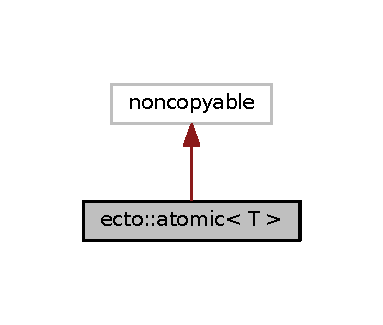
\includegraphics[width=184pt]{classecto_1_1atomic__inherit__graph}
\end{center}
\end{figure}


Collaboration diagram for ecto\+:\+:atomic$<$ T $>$\+:\nopagebreak
\begin{figure}[H]
\begin{center}
\leavevmode
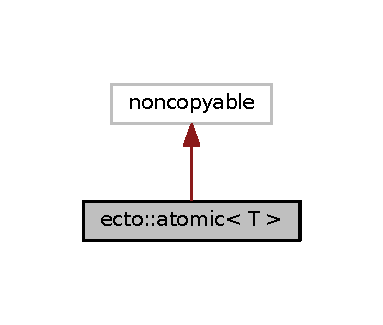
\includegraphics[width=184pt]{classecto_1_1atomic__coll__graph}
\end{center}
\end{figure}
\subsection*{Classes}
\begin{DoxyCompactItemize}
\item 
class \hyperlink{classecto_1_1atomic_1_1scoped__lock}{scoped\+\_\+lock}
\end{DoxyCompactItemize}
\subsection*{Public Member Functions}
\begin{DoxyCompactItemize}
\item 
\hyperlink{classecto_1_1atomic_ab905c76c87a64092b9c4217c6cc2b00d}{atomic} ()
\item 
\hyperlink{classecto_1_1atomic_a805df2159911558f653edbe19a789b51}{atomic} (T v)
\item 
T \hyperlink{classecto_1_1atomic_aa98175bf31ad55fe61e5d3d324a4f664}{get} ()
\end{DoxyCompactItemize}
\subsection*{Private Attributes}
\begin{DoxyCompactItemize}
\item 
T \hyperlink{classecto_1_1atomic_ac5ba45af623c7bc47e6918e290e39c67}{value}
\item 
boost\+::mutex \hyperlink{classecto_1_1atomic_a52a121e21f9449371998dbccaca0cbde}{mtx}
\end{DoxyCompactItemize}


\subsection{Constructor \& Destructor Documentation}
\index{ecto\+::atomic@{ecto\+::atomic}!atomic@{atomic}}
\index{atomic@{atomic}!ecto\+::atomic@{ecto\+::atomic}}
\subsubsection[{\texorpdfstring{atomic()}{atomic()}}]{\setlength{\rightskip}{0pt plus 5cm}template$<$typename T $>$ {\bf ecto\+::atomic}$<$ T $>$\+::{\bf atomic} (
\begin{DoxyParamCaption}
{}
\end{DoxyParamCaption}
)\hspace{0.3cm}{\ttfamily [inline]}}\hypertarget{classecto_1_1atomic_ab905c76c87a64092b9c4217c6cc2b00d}{}\label{classecto_1_1atomic_ab905c76c87a64092b9c4217c6cc2b00d}
\index{ecto\+::atomic@{ecto\+::atomic}!atomic@{atomic}}
\index{atomic@{atomic}!ecto\+::atomic@{ecto\+::atomic}}
\subsubsection[{\texorpdfstring{atomic(\+T v)}{atomic(T v)}}]{\setlength{\rightskip}{0pt plus 5cm}template$<$typename T $>$ {\bf ecto\+::atomic}$<$ T $>$\+::{\bf atomic} (
\begin{DoxyParamCaption}
\item[{T}]{v}
\end{DoxyParamCaption}
)\hspace{0.3cm}{\ttfamily [inline]}, {\ttfamily [explicit]}}\hypertarget{classecto_1_1atomic_a805df2159911558f653edbe19a789b51}{}\label{classecto_1_1atomic_a805df2159911558f653edbe19a789b51}


\subsection{Member Function Documentation}
\index{ecto\+::atomic@{ecto\+::atomic}!get@{get}}
\index{get@{get}!ecto\+::atomic@{ecto\+::atomic}}
\subsubsection[{\texorpdfstring{get()}{get()}}]{\setlength{\rightskip}{0pt plus 5cm}template$<$typename T $>$ T {\bf ecto\+::atomic}$<$ T $>$\+::get (
\begin{DoxyParamCaption}
{}
\end{DoxyParamCaption}
)\hspace{0.3cm}{\ttfamily [inline]}}\hypertarget{classecto_1_1atomic_aa98175bf31ad55fe61e5d3d324a4f664}{}\label{classecto_1_1atomic_aa98175bf31ad55fe61e5d3d324a4f664}


\subsection{Member Data Documentation}
\index{ecto\+::atomic@{ecto\+::atomic}!mtx@{mtx}}
\index{mtx@{mtx}!ecto\+::atomic@{ecto\+::atomic}}
\subsubsection[{\texorpdfstring{mtx}{mtx}}]{\setlength{\rightskip}{0pt plus 5cm}template$<$typename T $>$ boost\+::mutex {\bf ecto\+::atomic}$<$ T $>$\+::mtx\hspace{0.3cm}{\ttfamily [private]}}\hypertarget{classecto_1_1atomic_a52a121e21f9449371998dbccaca0cbde}{}\label{classecto_1_1atomic_a52a121e21f9449371998dbccaca0cbde}
\index{ecto\+::atomic@{ecto\+::atomic}!value@{value}}
\index{value@{value}!ecto\+::atomic@{ecto\+::atomic}}
\subsubsection[{\texorpdfstring{value}{value}}]{\setlength{\rightskip}{0pt plus 5cm}template$<$typename T $>$ T {\bf ecto\+::atomic}$<$ T $>$\+::value\hspace{0.3cm}{\ttfamily [private]}}\hypertarget{classecto_1_1atomic_ac5ba45af623c7bc47e6918e290e39c67}{}\label{classecto_1_1atomic_ac5ba45af623c7bc47e6918e290e39c67}


The documentation for this class was generated from the following file\+:\begin{DoxyCompactItemize}
\item 
/home/vrabaud/workspace/recognition\+\_\+kitchen/src/ecto/include/ecto/\hyperlink{atomic_8hpp}{atomic.\+hpp}\end{DoxyCompactItemize}

\hypertarget{structecto_1_1bounded}{}\section{ecto\+:\+:bounded$<$ T $>$ Struct Template Reference}
\label{structecto_1_1bounded}\index{ecto\+::bounded$<$ T $>$@{ecto\+::bounded$<$ T $>$}}


{\ttfamily \#include $<$parameters.\+hpp$>$}

\subsection*{Public Member Functions}
\begin{DoxyCompactItemize}
\item 
\hyperlink{structecto_1_1bounded_a2b27e0fe3fd9bd4392fe0422328cdc21}{bounded} (const T \&\hyperlink{structecto_1_1bounded_a92b4f90f8588d99f0d6d3216565c3f82}{value}, const T \&\hyperlink{structecto_1_1bounded_a1809a5fa7b57a025107b0c12e6a293ae}{min}, const T \&\hyperlink{structecto_1_1bounded_a8df1ae15c7a45a33bb17f8482c81418b}{max})
\item 
\hyperlink{structecto_1_1bounded_a77b53af4586fb05eb2f9e4b0f350b42d}{bounded} (const T \&\hyperlink{structecto_1_1bounded_a92b4f90f8588d99f0d6d3216565c3f82}{value})
\item 
\hyperlink{structecto_1_1bounded}{bounded} \& \hyperlink{structecto_1_1bounded_a3c8158a8581de90b22f1f702b47d4c78}{operator=} (const T \&\hyperlink{structecto_1_1bounded_a92b4f90f8588d99f0d6d3216565c3f82}{value})
\item 
void \hyperlink{structecto_1_1bounded_aff81e7792f2b05be160cd0d8cde73023}{set} (const T \&\hyperlink{structecto_1_1bounded_a92b4f90f8588d99f0d6d3216565c3f82}{value})
\item 
bool \hyperlink{structecto_1_1bounded_a7d73cabf049b631f8abc9973a2bff183}{check} (const T \&\hyperlink{structecto_1_1bounded_a92b4f90f8588d99f0d6d3216565c3f82}{value}) const 
\item 
std\+::string \hyperlink{structecto_1_1bounded_a929439a21225157ab7ba7f4427dc42ad}{bounds} () const 
\item 
\hyperlink{structecto_1_1bounded_ae032eb9fc9ba64687a249f50a7bdf877}{operator T} () const 
\end{DoxyCompactItemize}
\subsection*{Public Attributes}
\begin{DoxyCompactItemize}
\item 
T \hyperlink{structecto_1_1bounded_a92b4f90f8588d99f0d6d3216565c3f82}{value}
\item 
T \hyperlink{structecto_1_1bounded_a1809a5fa7b57a025107b0c12e6a293ae}{min}
\item 
T \hyperlink{structecto_1_1bounded_a8df1ae15c7a45a33bb17f8482c81418b}{max}
\item 
bool \hyperlink{structecto_1_1bounded_ab7ddb1af2438b94a3563f00188d02690}{has\+\_\+bounds}
\end{DoxyCompactItemize}


\subsection{Constructor \& Destructor Documentation}
\hypertarget{structecto_1_1bounded_a2b27e0fe3fd9bd4392fe0422328cdc21}{}\index{ecto\+::bounded@{ecto\+::bounded}!bounded@{bounded}}
\index{bounded@{bounded}!ecto\+::bounded@{ecto\+::bounded}}
\subsubsection[{bounded}]{\setlength{\rightskip}{0pt plus 5cm}template$<$typename T $>$ {\bf ecto\+::bounded}$<$ T $>$\+::{\bf bounded} (
\begin{DoxyParamCaption}
\item[{const T \&}]{value, }
\item[{const T \&}]{min, }
\item[{const T \&}]{max}
\end{DoxyParamCaption}
)}\label{structecto_1_1bounded_a2b27e0fe3fd9bd4392fe0422328cdc21}
\hypertarget{structecto_1_1bounded_a77b53af4586fb05eb2f9e4b0f350b42d}{}\index{ecto\+::bounded@{ecto\+::bounded}!bounded@{bounded}}
\index{bounded@{bounded}!ecto\+::bounded@{ecto\+::bounded}}
\subsubsection[{bounded}]{\setlength{\rightskip}{0pt plus 5cm}template$<$typename T $>$ {\bf ecto\+::bounded}$<$ T $>$\+::{\bf bounded} (
\begin{DoxyParamCaption}
\item[{const T \&}]{value}
\end{DoxyParamCaption}
)\hspace{0.3cm}{\ttfamily [explicit]}}\label{structecto_1_1bounded_a77b53af4586fb05eb2f9e4b0f350b42d}


\subsection{Member Function Documentation}
\hypertarget{structecto_1_1bounded_a929439a21225157ab7ba7f4427dc42ad}{}\index{ecto\+::bounded@{ecto\+::bounded}!bounds@{bounds}}
\index{bounds@{bounds}!ecto\+::bounded@{ecto\+::bounded}}
\subsubsection[{bounds}]{\setlength{\rightskip}{0pt plus 5cm}template$<$typename T $>$ std\+::string {\bf ecto\+::bounded}$<$ T $>$\+::bounds (
\begin{DoxyParamCaption}
{}
\end{DoxyParamCaption}
) const}\label{structecto_1_1bounded_a929439a21225157ab7ba7f4427dc42ad}
\hypertarget{structecto_1_1bounded_a7d73cabf049b631f8abc9973a2bff183}{}\index{ecto\+::bounded@{ecto\+::bounded}!check@{check}}
\index{check@{check}!ecto\+::bounded@{ecto\+::bounded}}
\subsubsection[{check}]{\setlength{\rightskip}{0pt plus 5cm}template$<$typename T $>$ bool {\bf ecto\+::bounded}$<$ T $>$\+::check (
\begin{DoxyParamCaption}
\item[{const T \&}]{value}
\end{DoxyParamCaption}
) const}\label{structecto_1_1bounded_a7d73cabf049b631f8abc9973a2bff183}
\hypertarget{structecto_1_1bounded_ae032eb9fc9ba64687a249f50a7bdf877}{}\index{ecto\+::bounded@{ecto\+::bounded}!operator T@{operator T}}
\index{operator T@{operator T}!ecto\+::bounded@{ecto\+::bounded}}
\subsubsection[{operator T}]{\setlength{\rightskip}{0pt plus 5cm}template$<$typename T $>$ {\bf ecto\+::bounded}$<$ T $>$\+::operator T (
\begin{DoxyParamCaption}
{}
\end{DoxyParamCaption}
) const}\label{structecto_1_1bounded_ae032eb9fc9ba64687a249f50a7bdf877}
\hypertarget{structecto_1_1bounded_a3c8158a8581de90b22f1f702b47d4c78}{}\index{ecto\+::bounded@{ecto\+::bounded}!operator=@{operator=}}
\index{operator=@{operator=}!ecto\+::bounded@{ecto\+::bounded}}
\subsubsection[{operator=}]{\setlength{\rightskip}{0pt plus 5cm}template$<$typename T $>$ {\bf bounded}$<$ T $>$ \& {\bf ecto\+::bounded}$<$ T $>$\+::operator= (
\begin{DoxyParamCaption}
\item[{const T \&}]{value}
\end{DoxyParamCaption}
)}\label{structecto_1_1bounded_a3c8158a8581de90b22f1f702b47d4c78}
\hypertarget{structecto_1_1bounded_aff81e7792f2b05be160cd0d8cde73023}{}\index{ecto\+::bounded@{ecto\+::bounded}!set@{set}}
\index{set@{set}!ecto\+::bounded@{ecto\+::bounded}}
\subsubsection[{set}]{\setlength{\rightskip}{0pt plus 5cm}template$<$typename T $>$ void {\bf ecto\+::bounded}$<$ T $>$\+::set (
\begin{DoxyParamCaption}
\item[{const T \&}]{value}
\end{DoxyParamCaption}
)}\label{structecto_1_1bounded_aff81e7792f2b05be160cd0d8cde73023}


\subsection{Member Data Documentation}
\hypertarget{structecto_1_1bounded_ab7ddb1af2438b94a3563f00188d02690}{}\index{ecto\+::bounded@{ecto\+::bounded}!has\+\_\+bounds@{has\+\_\+bounds}}
\index{has\+\_\+bounds@{has\+\_\+bounds}!ecto\+::bounded@{ecto\+::bounded}}
\subsubsection[{has\+\_\+bounds}]{\setlength{\rightskip}{0pt plus 5cm}template$<$typename T $>$ bool {\bf ecto\+::bounded}$<$ T $>$\+::has\+\_\+bounds}\label{structecto_1_1bounded_ab7ddb1af2438b94a3563f00188d02690}
\hypertarget{structecto_1_1bounded_a8df1ae15c7a45a33bb17f8482c81418b}{}\index{ecto\+::bounded@{ecto\+::bounded}!max@{max}}
\index{max@{max}!ecto\+::bounded@{ecto\+::bounded}}
\subsubsection[{max}]{\setlength{\rightskip}{0pt plus 5cm}template$<$typename T $>$ T {\bf ecto\+::bounded}$<$ T $>$\+::max}\label{structecto_1_1bounded_a8df1ae15c7a45a33bb17f8482c81418b}
\hypertarget{structecto_1_1bounded_a1809a5fa7b57a025107b0c12e6a293ae}{}\index{ecto\+::bounded@{ecto\+::bounded}!min@{min}}
\index{min@{min}!ecto\+::bounded@{ecto\+::bounded}}
\subsubsection[{min}]{\setlength{\rightskip}{0pt plus 5cm}template$<$typename T $>$ T {\bf ecto\+::bounded}$<$ T $>$\+::min}\label{structecto_1_1bounded_a1809a5fa7b57a025107b0c12e6a293ae}
\hypertarget{structecto_1_1bounded_a92b4f90f8588d99f0d6d3216565c3f82}{}\index{ecto\+::bounded@{ecto\+::bounded}!value@{value}}
\index{value@{value}!ecto\+::bounded@{ecto\+::bounded}}
\subsubsection[{value}]{\setlength{\rightskip}{0pt plus 5cm}template$<$typename T $>$ T {\bf ecto\+::bounded}$<$ T $>$\+::value}\label{structecto_1_1bounded_a92b4f90f8588d99f0d6d3216565c3f82}


The documentation for this struct was generated from the following file\+:\begin{DoxyCompactItemize}
\item 
/home/vrabaud/workspace/recognition\+\_\+kitchen/src/ecto/include/ecto/\hyperlink{parameters_8hpp}{parameters.\+hpp}\end{DoxyCompactItemize}

\hypertarget{structecto_1_1tendril_1_1Caller}{\section{ecto\-:\-:tendril\-:\-:Caller$<$ T $>$ Struct Template Reference}
\label{structecto_1_1tendril_1_1Caller}\index{ecto\-::tendril\-::\-Caller$<$ T $>$@{ecto\-::tendril\-::\-Caller$<$ T $>$}}
}


{\ttfamily \#include $<$tendril.\-hpp$>$}

\subsection*{Public Types}
\begin{DoxyCompactItemize}
\item 
typedef boost\-::function1$<$ void, T $>$ \hyperlink{structecto_1_1tendril_1_1Caller_a846333ac5c22cfb6eafb1c2240c0c623}{Cb\-T}
\end{DoxyCompactItemize}
\subsection*{Public Member Functions}
\begin{DoxyCompactItemize}
\item 
\hyperlink{structecto_1_1tendril_1_1Caller_a84b71a5526ff59dcbd6cb7a102f8d9db}{Caller} (\hyperlink{structecto_1_1tendril_1_1Caller_a846333ac5c22cfb6eafb1c2240c0c623}{Cb\-T} \hyperlink{structecto_1_1tendril_1_1Caller_afecdbc09ca504c16292a6365ab1cd950}{cb})
\item 
void \hyperlink{structecto_1_1tendril_1_1Caller_a19099e68a2059823575e71f45b2c0b20}{operator()} (\hyperlink{classecto_1_1tendril}{tendril} \&t)
\end{DoxyCompactItemize}
\subsection*{Public Attributes}
\begin{DoxyCompactItemize}
\item 
\hyperlink{structecto_1_1tendril_1_1Caller_a846333ac5c22cfb6eafb1c2240c0c623}{Cb\-T} \hyperlink{structecto_1_1tendril_1_1Caller_afecdbc09ca504c16292a6365ab1cd950}{cb}
\end{DoxyCompactItemize}


\subsection{Member Typedef Documentation}
\hypertarget{structecto_1_1tendril_1_1Caller_a846333ac5c22cfb6eafb1c2240c0c623}{\index{ecto\-::tendril\-::\-Caller@{ecto\-::tendril\-::\-Caller}!Cb\-T@{Cb\-T}}
\index{Cb\-T@{Cb\-T}!ecto::tendril::Caller@{ecto\-::tendril\-::\-Caller}}
\subsubsection[{Cb\-T}]{\setlength{\rightskip}{0pt plus 5cm}template$<$typename T $>$ typedef boost\-::function1$<$void, T$>$ {\bf ecto\-::tendril\-::\-Caller}$<$ T $>$\-::{\bf Cb\-T}}}\label{structecto_1_1tendril_1_1Caller_a846333ac5c22cfb6eafb1c2240c0c623}


\subsection{Constructor \& Destructor Documentation}
\hypertarget{structecto_1_1tendril_1_1Caller_a84b71a5526ff59dcbd6cb7a102f8d9db}{\index{ecto\-::tendril\-::\-Caller@{ecto\-::tendril\-::\-Caller}!Caller@{Caller}}
\index{Caller@{Caller}!ecto::tendril::Caller@{ecto\-::tendril\-::\-Caller}}
\subsubsection[{Caller}]{\setlength{\rightskip}{0pt plus 5cm}template$<$typename T $>$ {\bf ecto\-::tendril\-::\-Caller}$<$ T $>$\-::{\bf Caller} (
\begin{DoxyParamCaption}
\item[{{\bf Cb\-T}}]{cb}
\end{DoxyParamCaption}
)\hspace{0.3cm}{\ttfamily [inline]}}}\label{structecto_1_1tendril_1_1Caller_a84b71a5526ff59dcbd6cb7a102f8d9db}


\subsection{Member Function Documentation}
\hypertarget{structecto_1_1tendril_1_1Caller_a19099e68a2059823575e71f45b2c0b20}{\index{ecto\-::tendril\-::\-Caller@{ecto\-::tendril\-::\-Caller}!operator()@{operator()}}
\index{operator()@{operator()}!ecto::tendril::Caller@{ecto\-::tendril\-::\-Caller}}
\subsubsection[{operator()}]{\setlength{\rightskip}{0pt plus 5cm}template$<$typename T $>$ void {\bf ecto\-::tendril\-::\-Caller}$<$ T $>$\-::operator() (
\begin{DoxyParamCaption}
\item[{{\bf tendril} \&}]{t}
\end{DoxyParamCaption}
)\hspace{0.3cm}{\ttfamily [inline]}}}\label{structecto_1_1tendril_1_1Caller_a19099e68a2059823575e71f45b2c0b20}


\subsection{Member Data Documentation}
\hypertarget{structecto_1_1tendril_1_1Caller_afecdbc09ca504c16292a6365ab1cd950}{\index{ecto\-::tendril\-::\-Caller@{ecto\-::tendril\-::\-Caller}!cb@{cb}}
\index{cb@{cb}!ecto::tendril::Caller@{ecto\-::tendril\-::\-Caller}}
\subsubsection[{cb}]{\setlength{\rightskip}{0pt plus 5cm}template$<$typename T $>$ {\bf Cb\-T} {\bf ecto\-::tendril\-::\-Caller}$<$ T $>$\-::cb}}\label{structecto_1_1tendril_1_1Caller_afecdbc09ca504c16292a6365ab1cd950}


The documentation for this struct was generated from the following file\-:\begin{DoxyCompactItemize}
\item 
/home/vrabaud/workspace/recognition\-\_\-kitchen/src/ecto/include/ecto/\hyperlink{tendril_8hpp}{tendril.\-hpp}\end{DoxyCompactItemize}

\hypertarget{structecto_1_1cell}{\section{ecto\-:\-:cell Struct Reference}
\label{structecto_1_1cell}\index{ecto\-::cell@{ecto\-::cell}}
}


\hyperlink{structecto_1_1cell}{ecto\-::cell} is the non virtual interface to the basic building block of ecto graphs. This interface should never be the parent of client cell, but may be used for polymorphic access to client cells.  




{\ttfamily \#include $<$cell.\-hpp$>$}



Inheritance diagram for ecto\-:\-:cell\-:\nopagebreak
\begin{figure}[H]
\begin{center}
\leavevmode
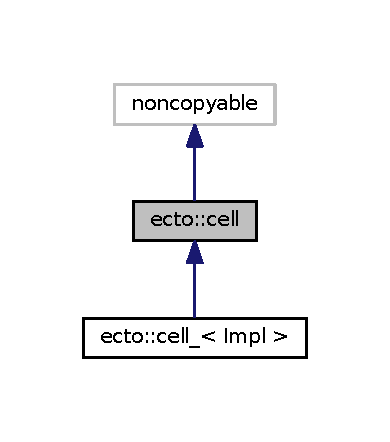
\includegraphics[width=186pt]{structecto_1_1cell__inherit__graph}
\end{center}
\end{figure}


Collaboration diagram for ecto\-:\-:cell\-:\nopagebreak
\begin{figure}[H]
\begin{center}
\leavevmode
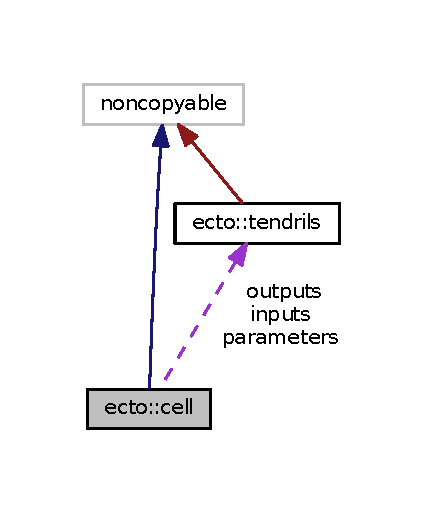
\includegraphics[width=203pt]{structecto_1_1cell__coll__graph}
\end{center}
\end{figure}
\subsection*{Public Types}
\begin{DoxyCompactItemize}
\item 
typedef boost\-::shared\-\_\-ptr$<$ \hyperlink{structecto_1_1cell}{cell} $>$ \hyperlink{structecto_1_1cell_af2cab9d2bc012088c4f58c40da57a862}{ptr}
\begin{DoxyCompactList}\small\item\em A convenience pointer typedef. \end{DoxyCompactList}\end{DoxyCompactItemize}
\subsection*{Public Member Functions}
\begin{DoxyCompactItemize}
\item 
\hyperlink{structecto_1_1cell_a782c9d0f521f8a34c8eed309d0d8d79a}{cell} ()
\item 
virtual \hyperlink{structecto_1_1cell_a98748014df1b1a4fd3fbb47f6adc8c5e}{$\sim$cell} ()
\item 
void \hyperlink{structecto_1_1cell_a5c3c204f531de15920cb9d3db3ecfc4c}{declare\-\_\-params} ()
\begin{DoxyCompactList}\small\item\em Dispatches parameter declaration code. After this code, the parameters for the cell will be set to their defaults. \end{DoxyCompactList}\item 
void \hyperlink{structecto_1_1cell_af6c3782ed0d1c258bcf5050b4af272b4}{declare\-\_\-io} ()
\begin{DoxyCompactList}\small\item\em Dispatches input/output declaration code. It is assumed that the parameters have been declared before this is called, so that inputs and outputs may be dependent on those parameters. \end{DoxyCompactList}\item 
void \hyperlink{structecto_1_1cell_a30d48d21d6ffa86af4888f78e92241af}{configure} ()
\begin{DoxyCompactList}\small\item\em Given initialized parameters,inputs, and outputs, this will dispatch the client configuration code. This will allocated an instace of the clients cell, so this should not be called during introspection. \end{DoxyCompactList}\item 
void \hyperlink{structecto_1_1cell_a0416d7265db282a18202b58636be7165}{activate} ()
\begin{DoxyCompactList}\small\item\em Activate the cell. i.\-e. Put it into a \char`\"{}ready\char`\"{} state, opening sockets, etc. \end{DoxyCompactList}\item 
void \hyperlink{structecto_1_1cell_ab988f785fb943af3ff48c2d6f67a07aa}{deactivate} ()
\begin{DoxyCompactList}\small\item\em Deactivate the cell. i.\-e. Put it into an \char`\"{}unready\char`\"{} state, closing sockets, etc. \end{DoxyCompactList}\item 
void \hyperlink{structecto_1_1cell_a06abb010763ff7aeaaf2b28be4a6424a}{start} ()
\item 
void \hyperlink{structecto_1_1cell_abac52b774d350b02dc99a55c64b94bcd}{stop} ()
\item 
\hyperlink{namespaceecto_a93d82cd28db695d53963fb696582762c}{Return\-Code} \hyperlink{structecto_1_1cell_a6b810671ee21f5dddbc1206abfb999f3}{process} ()
\begin{DoxyCompactList}\small\item\em Dispatches the process function for the client cell. This should only be called from one thread at a time. Also, this function may throw exceptions... \end{DoxyCompactList}\item 
\hyperlink{namespaceecto_a93d82cd28db695d53963fb696582762c}{Return\-Code} \hyperlink{structecto_1_1cell_a407e320190ee98c1a1a3042ac3c38f0e}{process\-\_\-with\-\_\-only\-\_\-these\-\_\-inputs} (const \hyperlink{classecto_1_1tendrils}{tendrils} \&connected\-\_\-inputs)
\item 
std\-::string \hyperlink{structecto_1_1cell_ae3b84af61e78dab25f66a66773d5c5df}{type} () const 
\begin{DoxyCompactList}\small\item\em Return the type of the child class. \end{DoxyCompactList}\item 
std\-::string \hyperlink{structecto_1_1cell_a931fbc02fff66a58684ab25e00dbb2f8}{name} () const 
\begin{DoxyCompactList}\small\item\em Grab the name of the instance. \end{DoxyCompactList}\item 
void \hyperlink{structecto_1_1cell_a3956efb238f50a6983b86f430c47ca05}{name} (const std\-::string \&name)
\begin{DoxyCompactList}\small\item\em Set the name of the instance. \end{DoxyCompactList}\item 
std\-::string \hyperlink{structecto_1_1cell_aefa443962201caebb08d1a3163730639}{short\-\_\-doc} () const 
\begin{DoxyCompactList}\small\item\em Set the short\-\_\-doc\-\_\- of the instance. \end{DoxyCompactList}\item 
void \hyperlink{structecto_1_1cell_a49d510eec19d352c5729e6a2fd149340}{short\-\_\-doc} (const std\-::string \&short\-\_\-doc)
\begin{DoxyCompactList}\small\item\em Set the short\-\_\-doc\-\_\- of the instance. \end{DoxyCompactList}\item 
void \hyperlink{structecto_1_1cell_af32a9e2113b7afcb5b225bdc3c234e8c}{reset\-\_\-strand} ()
\item 
void \hyperlink{structecto_1_1cell_ae0009fc4a4d12d400126f455396f5c9f}{set\-\_\-strand} (\hyperlink{structecto_1_1strand}{ecto\-::strand})
\item 
std\-::string \hyperlink{structecto_1_1cell_a486454d7466c5f0373ecb42dd4e97b2f}{gen\-\_\-doc} (const std\-::string \&doc=\char`\"{}A module...\char`\"{}) const 
\begin{DoxyCompactList}\small\item\em Generate an Restructured Text doc string for the cell. Includes documentation for all parameters, inputs, outputs. \end{DoxyCompactList}\item 
void \hyperlink{structecto_1_1cell_aa03c0f569bb4b14e81f4d2a8747273e5}{verify\-\_\-params} () const 
\item 
void \hyperlink{structecto_1_1cell_aed712e80344ce04dbb9105bb6a1aa53a}{verify\-\_\-inputs} () const 
\item 
bool \hyperlink{structecto_1_1cell_ab1dfafd237e0adf273af65d549e7516e}{process\-\_\-connected\-\_\-inputs\-\_\-only} () const 
\begin{DoxyCompactList}\small\item\em Processing mode query -\/ only connected tendrils or all. Typically used by the scheduler to arrange input tendrils when invoking a process. \end{DoxyCompactList}\item 
void \hyperlink{structecto_1_1cell_a4c42ef400acac92d825e7dc25ff53bdc}{set\-\_\-process\-\_\-connected\-\_\-inputs\-\_\-only} (const bool \&value)
\item 
\hyperlink{structecto_1_1cell_af2cab9d2bc012088c4f58c40da57a862}{ptr} \hyperlink{structecto_1_1cell_a213dabd285300f5d4c7e0f5fd6142e81}{clone} () const 
\item 
virtual bool \hyperlink{structecto_1_1cell_ab9a6c3fd8f76289f338a9e05368b1aff}{init} ()=0
\end{DoxyCompactItemize}
\subsection*{Public Attributes}
\begin{DoxyCompactItemize}
\item 
\hyperlink{classecto_1_1tendrils}{tendrils} \hyperlink{structecto_1_1cell_ae00a91199c758cf7c24dcf0ecdf70a27}{parameters}
\begin{DoxyCompactList}\small\item\em Parameters. \end{DoxyCompactList}\item 
\hyperlink{classecto_1_1tendrils}{tendrils} \hyperlink{structecto_1_1cell_a65099b0458a7761b8bfa7a1ddc17e92f}{inputs}
\begin{DoxyCompactList}\small\item\em Inputs, inboxes, always have a valid value ( may be N\-U\-L\-L ) \end{DoxyCompactList}\item 
\hyperlink{classecto_1_1tendrils}{tendrils} \hyperlink{structecto_1_1cell_a93951743b603faba35312ebdb07ceb22}{outputs}
\begin{DoxyCompactList}\small\item\em Outputs, outboxes, always have a valid value ( may be N\-U\-L\-L ) \end{DoxyCompactList}\item 
boost\-::optional$<$ \hyperlink{structecto_1_1strand}{strand} $>$ \hyperlink{structecto_1_1cell_ada052f06257277c1b53c82226dff5821}{strand\-\_\-}
\begin{DoxyCompactList}\small\item\em The strand that this cell should be executed in. \end{DoxyCompactList}\end{DoxyCompactItemize}
\subsection*{Protected Member Functions}
\begin{DoxyCompactItemize}
\item 
virtual void \hyperlink{structecto_1_1cell_abcf3cc29703214a7ede63d652e17ee96}{dispatch\-\_\-declare\-\_\-params} (\hyperlink{classecto_1_1tendrils}{tendrils} \&t)=0
\item 
virtual void \hyperlink{structecto_1_1cell_acb4cdb70f2db329ba9c615d74c63a4b2}{dispatch\-\_\-declare\-\_\-io} (const \hyperlink{classecto_1_1tendrils}{tendrils} \&params, \hyperlink{classecto_1_1tendrils}{tendrils} \&\hyperlink{structecto_1_1cell_a65099b0458a7761b8bfa7a1ddc17e92f}{inputs}, \hyperlink{classecto_1_1tendrils}{tendrils} \&\hyperlink{structecto_1_1cell_a93951743b603faba35312ebdb07ceb22}{outputs})=0
\item 
virtual void \hyperlink{structecto_1_1cell_a19c7c679dededd37ace918bf0ff31cd3}{dispatch\-\_\-configure} (const \hyperlink{classecto_1_1tendrils}{tendrils} \&params, const \hyperlink{classecto_1_1tendrils}{tendrils} \&\hyperlink{structecto_1_1cell_a65099b0458a7761b8bfa7a1ddc17e92f}{inputs}, const \hyperlink{classecto_1_1tendrils}{tendrils} \&\hyperlink{structecto_1_1cell_a93951743b603faba35312ebdb07ceb22}{outputs})=0
\item 
virtual void \hyperlink{structecto_1_1cell_aa345ec700e5e213364c7bb20571cd78d}{dispatch\-\_\-activate} ()=0
\item 
virtual void \hyperlink{structecto_1_1cell_a4b5f111fc7b90dccce0cd70e28c9be62}{dispatch\-\_\-deactivate} ()=0
\item 
virtual \hyperlink{namespaceecto_a93d82cd28db695d53963fb696582762c}{Return\-Code} \hyperlink{structecto_1_1cell_a390bd83cfdff120523efc5c3e76bc3e5}{dispatch\-\_\-process} (const \hyperlink{classecto_1_1tendrils}{tendrils} \&\hyperlink{structecto_1_1cell_a65099b0458a7761b8bfa7a1ddc17e92f}{inputs}, const \hyperlink{classecto_1_1tendrils}{tendrils} \&\hyperlink{structecto_1_1cell_a93951743b603faba35312ebdb07ceb22}{outputs})=0
\item 
virtual void \hyperlink{structecto_1_1cell_ab5c75358dd32fa811116654bdc76385b}{dispatch\-\_\-start} ()=0
\item 
virtual void \hyperlink{structecto_1_1cell_a65ff7141e927a7115a785478a03b94bc}{dispatch\-\_\-stop} ()=0
\item 
virtual std\-::string \hyperlink{structecto_1_1cell_a456b56e3291f5e2bb68ce31a4a43ece5}{dispatch\-\_\-name} () const =0
\item 
virtual \hyperlink{structecto_1_1cell_af2cab9d2bc012088c4f58c40da57a862}{ptr} \hyperlink{structecto_1_1cell_a7beccd749c33bd8b4c5827598e8fe5a5}{dispatch\-\_\-clone} () const =0
\item 
virtual std\-::string \hyperlink{structecto_1_1cell_a400b8aecf15588cfb21d712fbb000e8a}{dispatch\-\_\-short\-\_\-doc} () const 
\item 
virtual void \hyperlink{structecto_1_1cell_a407d24db843ffe12ac57c9a8827a9fe8}{dispatch\-\_\-short\-\_\-doc} (const std\-::string \&)
\end{DoxyCompactItemize}
\subsection*{Private Member Functions}
\begin{DoxyCompactItemize}
\item 
\hyperlink{structecto_1_1cell_ac0ae6a72cecf48916bb6dd1b6393d1b3}{cell} (const \hyperlink{structecto_1_1cell}{cell} \&)
\end{DoxyCompactItemize}
\subsection*{Private Attributes}
\begin{DoxyCompactItemize}
\item 
std\-::string \hyperlink{structecto_1_1cell_a2bf4e65c7a699624c61d3b55cfac45ed}{instance\-\_\-name\-\_\-}
\item 
bool \hyperlink{structecto_1_1cell_a187d36610ae8035e9f589de06ecc0d0a}{configured\-\_\-}
\item 
bool \hyperlink{structecto_1_1cell_ad270620c006f30471b2371feb38b6a03}{activated\-\_\-}
\item 
bool \hyperlink{structecto_1_1cell_a9a9d7fa3bb72fd74073a997bfb6cbad8}{process\-\_\-connected\-\_\-inputs\-\_\-only\-\_\-}
\end{DoxyCompactItemize}


\subsection{Detailed Description}
\hyperlink{structecto_1_1cell}{ecto\-::cell} is the non virtual interface to the basic building block of ecto graphs. This interface should never be the parent of client cell, but may be used for polymorphic access to client cells. 

Clients should expose their code to this interface through ecto\-::wrap, or ecto\-::create\-\_\-cell$<$\-T$>$().

For a client's cell to satisfy the \hyperlink{structecto_1_1cell}{ecto\-::cell} idiom, it must look similar to the following definition. 
\begin{DoxyCode}
\textcolor{keyword}{struct }MyEctoCell
\{
  \textcolor{comment}{//called first thing, the user should declare their parameters in this}
  \textcolor{comment}{//free standing function.}
  \textcolor{keyword}{static} \textcolor{keywordtype}{void} \hyperlink{structecto_1_1cell_a5c3c204f531de15920cb9d3db3ecfc4c}{declare\_params}(tendrils& params);
  \textcolor{comment}{//declare inputs and outputs here. The parameters may be used to}
  \textcolor{comment}{//determine the io}
  \textcolor{keyword}{static} \textcolor{keywordtype}{void} \hyperlink{structecto_1_1cell_af6c3782ed0d1c258bcf5050b4af272b4}{declare\_io}(\textcolor{keyword}{const} tendrils& params, tendrils& in, tendrils& out);
  \textcolor{comment}{//called right after allocation of the cell, exactly once.}
  \textcolor{keywordtype}{void} \hyperlink{structecto_1_1cell_a30d48d21d6ffa86af4888f78e92241af}{configure}(tendrils& params, tendrils& \hyperlink{structecto_1_1cell_a65099b0458a7761b8bfa7a1ddc17e92f}{inputs}, tendrils& 
      \hyperlink{structecto_1_1cell_a93951743b603faba35312ebdb07ceb22}{outputs});
  \textcolor{comment}{//called at every execution of the graph}
  \textcolor{keywordtype}{int} \hyperlink{structecto_1_1cell_a6b810671ee21f5dddbc1206abfb999f3}{process}(\textcolor{keyword}{const} tendrils& in, tendrils& out);
\};
\end{DoxyCode}


All functions are optional. 

\subsection{Member Typedef Documentation}
\hypertarget{structecto_1_1cell_af2cab9d2bc012088c4f58c40da57a862}{\index{ecto\-::cell@{ecto\-::cell}!ptr@{ptr}}
\index{ptr@{ptr}!ecto::cell@{ecto\-::cell}}
\subsubsection[{ptr}]{\setlength{\rightskip}{0pt plus 5cm}typedef boost\-::shared\-\_\-ptr$<${\bf cell}$>$ {\bf ecto\-::cell\-::ptr}}}\label{structecto_1_1cell_af2cab9d2bc012088c4f58c40da57a862}


A convenience pointer typedef. 



\subsection{Constructor \& Destructor Documentation}
\hypertarget{structecto_1_1cell_a782c9d0f521f8a34c8eed309d0d8d79a}{\index{ecto\-::cell@{ecto\-::cell}!cell@{cell}}
\index{cell@{cell}!ecto::cell@{ecto\-::cell}}
\subsubsection[{cell}]{\setlength{\rightskip}{0pt plus 5cm}ecto\-::cell\-::cell (
\begin{DoxyParamCaption}
{}
\end{DoxyParamCaption}
)}}\label{structecto_1_1cell_a782c9d0f521f8a34c8eed309d0d8d79a}
\hypertarget{structecto_1_1cell_a98748014df1b1a4fd3fbb47f6adc8c5e}{\index{ecto\-::cell@{ecto\-::cell}!$\sim$cell@{$\sim$cell}}
\index{$\sim$cell@{$\sim$cell}!ecto::cell@{ecto\-::cell}}
\subsubsection[{$\sim$cell}]{\setlength{\rightskip}{0pt plus 5cm}virtual ecto\-::cell\-::$\sim$cell (
\begin{DoxyParamCaption}
{}
\end{DoxyParamCaption}
)\hspace{0.3cm}{\ttfamily [virtual]}}}\label{structecto_1_1cell_a98748014df1b1a4fd3fbb47f6adc8c5e}
\hypertarget{structecto_1_1cell_ac0ae6a72cecf48916bb6dd1b6393d1b3}{\index{ecto\-::cell@{ecto\-::cell}!cell@{cell}}
\index{cell@{cell}!ecto::cell@{ecto\-::cell}}
\subsubsection[{cell}]{\setlength{\rightskip}{0pt plus 5cm}ecto\-::cell\-::cell (
\begin{DoxyParamCaption}
\item[{const {\bf cell} \&}]{}
\end{DoxyParamCaption}
)\hspace{0.3cm}{\ttfamily [private]}}}\label{structecto_1_1cell_ac0ae6a72cecf48916bb6dd1b6393d1b3}


\subsection{Member Function Documentation}
\hypertarget{structecto_1_1cell_a0416d7265db282a18202b58636be7165}{\index{ecto\-::cell@{ecto\-::cell}!activate@{activate}}
\index{activate@{activate}!ecto::cell@{ecto\-::cell}}
\subsubsection[{activate}]{\setlength{\rightskip}{0pt plus 5cm}void ecto\-::cell\-::activate (
\begin{DoxyParamCaption}
{}
\end{DoxyParamCaption}
)}}\label{structecto_1_1cell_a0416d7265db282a18202b58636be7165}


Activate the cell. i.\-e. Put it into a \char`\"{}ready\char`\"{} state, opening sockets, etc. 

\hypertarget{structecto_1_1cell_a213dabd285300f5d4c7e0f5fd6142e81}{\index{ecto\-::cell@{ecto\-::cell}!clone@{clone}}
\index{clone@{clone}!ecto::cell@{ecto\-::cell}}
\subsubsection[{clone}]{\setlength{\rightskip}{0pt plus 5cm}{\bf ptr} ecto\-::cell\-::clone (
\begin{DoxyParamCaption}
{}
\end{DoxyParamCaption}
) const}}\label{structecto_1_1cell_a213dabd285300f5d4c7e0f5fd6142e81}
\hypertarget{structecto_1_1cell_a30d48d21d6ffa86af4888f78e92241af}{\index{ecto\-::cell@{ecto\-::cell}!configure@{configure}}
\index{configure@{configure}!ecto::cell@{ecto\-::cell}}
\subsubsection[{configure}]{\setlength{\rightskip}{0pt plus 5cm}void ecto\-::cell\-::configure (
\begin{DoxyParamCaption}
{}
\end{DoxyParamCaption}
)}}\label{structecto_1_1cell_a30d48d21d6ffa86af4888f78e92241af}


Given initialized parameters,inputs, and outputs, this will dispatch the client configuration code. This will allocated an instace of the clients cell, so this should not be called during introspection. 

\hypertarget{structecto_1_1cell_ab988f785fb943af3ff48c2d6f67a07aa}{\index{ecto\-::cell@{ecto\-::cell}!deactivate@{deactivate}}
\index{deactivate@{deactivate}!ecto::cell@{ecto\-::cell}}
\subsubsection[{deactivate}]{\setlength{\rightskip}{0pt plus 5cm}void ecto\-::cell\-::deactivate (
\begin{DoxyParamCaption}
{}
\end{DoxyParamCaption}
)}}\label{structecto_1_1cell_ab988f785fb943af3ff48c2d6f67a07aa}


Deactivate the cell. i.\-e. Put it into an \char`\"{}unready\char`\"{} state, closing sockets, etc. 

\hypertarget{structecto_1_1cell_af6c3782ed0d1c258bcf5050b4af272b4}{\index{ecto\-::cell@{ecto\-::cell}!declare\-\_\-io@{declare\-\_\-io}}
\index{declare\-\_\-io@{declare\-\_\-io}!ecto::cell@{ecto\-::cell}}
\subsubsection[{declare\-\_\-io}]{\setlength{\rightskip}{0pt plus 5cm}void ecto\-::cell\-::declare\-\_\-io (
\begin{DoxyParamCaption}
{}
\end{DoxyParamCaption}
)}}\label{structecto_1_1cell_af6c3782ed0d1c258bcf5050b4af272b4}


Dispatches input/output declaration code. It is assumed that the parameters have been declared before this is called, so that inputs and outputs may be dependent on those parameters. 

\hypertarget{structecto_1_1cell_a5c3c204f531de15920cb9d3db3ecfc4c}{\index{ecto\-::cell@{ecto\-::cell}!declare\-\_\-params@{declare\-\_\-params}}
\index{declare\-\_\-params@{declare\-\_\-params}!ecto::cell@{ecto\-::cell}}
\subsubsection[{declare\-\_\-params}]{\setlength{\rightskip}{0pt plus 5cm}void ecto\-::cell\-::declare\-\_\-params (
\begin{DoxyParamCaption}
{}
\end{DoxyParamCaption}
)}}\label{structecto_1_1cell_a5c3c204f531de15920cb9d3db3ecfc4c}


Dispatches parameter declaration code. After this code, the parameters for the cell will be set to their defaults. 

\hypertarget{structecto_1_1cell_aa345ec700e5e213364c7bb20571cd78d}{\index{ecto\-::cell@{ecto\-::cell}!dispatch\-\_\-activate@{dispatch\-\_\-activate}}
\index{dispatch\-\_\-activate@{dispatch\-\_\-activate}!ecto::cell@{ecto\-::cell}}
\subsubsection[{dispatch\-\_\-activate}]{\setlength{\rightskip}{0pt plus 5cm}virtual void ecto\-::cell\-::dispatch\-\_\-activate (
\begin{DoxyParamCaption}
{}
\end{DoxyParamCaption}
)\hspace{0.3cm}{\ttfamily [protected]}, {\ttfamily [pure virtual]}}}\label{structecto_1_1cell_aa345ec700e5e213364c7bb20571cd78d}


Implemented in \hyperlink{structecto_1_1cell___a31437fcb5a15e57e8287719f48cecbdd}{ecto\-::cell\-\_\-$<$ Impl $>$}.

\hypertarget{structecto_1_1cell_a7beccd749c33bd8b4c5827598e8fe5a5}{\index{ecto\-::cell@{ecto\-::cell}!dispatch\-\_\-clone@{dispatch\-\_\-clone}}
\index{dispatch\-\_\-clone@{dispatch\-\_\-clone}!ecto::cell@{ecto\-::cell}}
\subsubsection[{dispatch\-\_\-clone}]{\setlength{\rightskip}{0pt plus 5cm}virtual {\bf ptr} ecto\-::cell\-::dispatch\-\_\-clone (
\begin{DoxyParamCaption}
{}
\end{DoxyParamCaption}
) const\hspace{0.3cm}{\ttfamily [protected]}, {\ttfamily [pure virtual]}}}\label{structecto_1_1cell_a7beccd749c33bd8b4c5827598e8fe5a5}


Implemented in \hyperlink{structecto_1_1cell___ae2868bb59ddb378cbe7b98fd4e776930}{ecto\-::cell\-\_\-$<$ Impl $>$}.

\hypertarget{structecto_1_1cell_a19c7c679dededd37ace918bf0ff31cd3}{\index{ecto\-::cell@{ecto\-::cell}!dispatch\-\_\-configure@{dispatch\-\_\-configure}}
\index{dispatch\-\_\-configure@{dispatch\-\_\-configure}!ecto::cell@{ecto\-::cell}}
\subsubsection[{dispatch\-\_\-configure}]{\setlength{\rightskip}{0pt plus 5cm}virtual void ecto\-::cell\-::dispatch\-\_\-configure (
\begin{DoxyParamCaption}
\item[{const {\bf tendrils} \&}]{params, }
\item[{const {\bf tendrils} \&}]{inputs, }
\item[{const {\bf tendrils} \&}]{outputs}
\end{DoxyParamCaption}
)\hspace{0.3cm}{\ttfamily [protected]}, {\ttfamily [pure virtual]}}}\label{structecto_1_1cell_a19c7c679dededd37ace918bf0ff31cd3}


Implemented in \hyperlink{structecto_1_1cell___a953e526cefd3c419a01717740eab9227}{ecto\-::cell\-\_\-$<$ Impl $>$}.

\hypertarget{structecto_1_1cell_a4b5f111fc7b90dccce0cd70e28c9be62}{\index{ecto\-::cell@{ecto\-::cell}!dispatch\-\_\-deactivate@{dispatch\-\_\-deactivate}}
\index{dispatch\-\_\-deactivate@{dispatch\-\_\-deactivate}!ecto::cell@{ecto\-::cell}}
\subsubsection[{dispatch\-\_\-deactivate}]{\setlength{\rightskip}{0pt plus 5cm}virtual void ecto\-::cell\-::dispatch\-\_\-deactivate (
\begin{DoxyParamCaption}
{}
\end{DoxyParamCaption}
)\hspace{0.3cm}{\ttfamily [protected]}, {\ttfamily [pure virtual]}}}\label{structecto_1_1cell_a4b5f111fc7b90dccce0cd70e28c9be62}


Implemented in \hyperlink{structecto_1_1cell___a71463eb5e248d29814066904e7f0d515}{ecto\-::cell\-\_\-$<$ Impl $>$}.

\hypertarget{structecto_1_1cell_acb4cdb70f2db329ba9c615d74c63a4b2}{\index{ecto\-::cell@{ecto\-::cell}!dispatch\-\_\-declare\-\_\-io@{dispatch\-\_\-declare\-\_\-io}}
\index{dispatch\-\_\-declare\-\_\-io@{dispatch\-\_\-declare\-\_\-io}!ecto::cell@{ecto\-::cell}}
\subsubsection[{dispatch\-\_\-declare\-\_\-io}]{\setlength{\rightskip}{0pt plus 5cm}virtual void ecto\-::cell\-::dispatch\-\_\-declare\-\_\-io (
\begin{DoxyParamCaption}
\item[{const {\bf tendrils} \&}]{params, }
\item[{{\bf tendrils} \&}]{inputs, }
\item[{{\bf tendrils} \&}]{outputs}
\end{DoxyParamCaption}
)\hspace{0.3cm}{\ttfamily [protected]}, {\ttfamily [pure virtual]}}}\label{structecto_1_1cell_acb4cdb70f2db329ba9c615d74c63a4b2}


Implemented in \hyperlink{structecto_1_1cell___ad95920d295860b791e3fa733fb0745db}{ecto\-::cell\-\_\-$<$ Impl $>$}.

\hypertarget{structecto_1_1cell_abcf3cc29703214a7ede63d652e17ee96}{\index{ecto\-::cell@{ecto\-::cell}!dispatch\-\_\-declare\-\_\-params@{dispatch\-\_\-declare\-\_\-params}}
\index{dispatch\-\_\-declare\-\_\-params@{dispatch\-\_\-declare\-\_\-params}!ecto::cell@{ecto\-::cell}}
\subsubsection[{dispatch\-\_\-declare\-\_\-params}]{\setlength{\rightskip}{0pt plus 5cm}virtual void ecto\-::cell\-::dispatch\-\_\-declare\-\_\-params (
\begin{DoxyParamCaption}
\item[{{\bf tendrils} \&}]{t}
\end{DoxyParamCaption}
)\hspace{0.3cm}{\ttfamily [protected]}, {\ttfamily [pure virtual]}}}\label{structecto_1_1cell_abcf3cc29703214a7ede63d652e17ee96}


Implemented in \hyperlink{structecto_1_1cell___a0e435a14e4cc1d5cd7d80a16f2776565}{ecto\-::cell\-\_\-$<$ Impl $>$}.

\hypertarget{structecto_1_1cell_a456b56e3291f5e2bb68ce31a4a43ece5}{\index{ecto\-::cell@{ecto\-::cell}!dispatch\-\_\-name@{dispatch\-\_\-name}}
\index{dispatch\-\_\-name@{dispatch\-\_\-name}!ecto::cell@{ecto\-::cell}}
\subsubsection[{dispatch\-\_\-name}]{\setlength{\rightskip}{0pt plus 5cm}virtual std\-::string ecto\-::cell\-::dispatch\-\_\-name (
\begin{DoxyParamCaption}
{}
\end{DoxyParamCaption}
) const\hspace{0.3cm}{\ttfamily [protected]}, {\ttfamily [pure virtual]}}}\label{structecto_1_1cell_a456b56e3291f5e2bb68ce31a4a43ece5}


Implemented in \hyperlink{structecto_1_1cell___a288dac8bba40036b3f3e6b0641833039}{ecto\-::cell\-\_\-$<$ Impl $>$}.

\hypertarget{structecto_1_1cell_a390bd83cfdff120523efc5c3e76bc3e5}{\index{ecto\-::cell@{ecto\-::cell}!dispatch\-\_\-process@{dispatch\-\_\-process}}
\index{dispatch\-\_\-process@{dispatch\-\_\-process}!ecto::cell@{ecto\-::cell}}
\subsubsection[{dispatch\-\_\-process}]{\setlength{\rightskip}{0pt plus 5cm}virtual {\bf Return\-Code} ecto\-::cell\-::dispatch\-\_\-process (
\begin{DoxyParamCaption}
\item[{const {\bf tendrils} \&}]{inputs, }
\item[{const {\bf tendrils} \&}]{outputs}
\end{DoxyParamCaption}
)\hspace{0.3cm}{\ttfamily [protected]}, {\ttfamily [pure virtual]}}}\label{structecto_1_1cell_a390bd83cfdff120523efc5c3e76bc3e5}


Implemented in \hyperlink{structecto_1_1cell___a1ddd0142b998f0de06a7992c5db27f16}{ecto\-::cell\-\_\-$<$ Impl $>$}.

\hypertarget{structecto_1_1cell_a400b8aecf15588cfb21d712fbb000e8a}{\index{ecto\-::cell@{ecto\-::cell}!dispatch\-\_\-short\-\_\-doc@{dispatch\-\_\-short\-\_\-doc}}
\index{dispatch\-\_\-short\-\_\-doc@{dispatch\-\_\-short\-\_\-doc}!ecto::cell@{ecto\-::cell}}
\subsubsection[{dispatch\-\_\-short\-\_\-doc}]{\setlength{\rightskip}{0pt plus 5cm}virtual std\-::string ecto\-::cell\-::dispatch\-\_\-short\-\_\-doc (
\begin{DoxyParamCaption}
{}
\end{DoxyParamCaption}
) const\hspace{0.3cm}{\ttfamily [inline]}, {\ttfamily [protected]}, {\ttfamily [virtual]}}}\label{structecto_1_1cell_a400b8aecf15588cfb21d712fbb000e8a}


Reimplemented in \hyperlink{structecto_1_1cell___aea843d10de8a002ada9a29bec2ecb815}{ecto\-::cell\-\_\-$<$ Impl $>$}.

\hypertarget{structecto_1_1cell_a407d24db843ffe12ac57c9a8827a9fe8}{\index{ecto\-::cell@{ecto\-::cell}!dispatch\-\_\-short\-\_\-doc@{dispatch\-\_\-short\-\_\-doc}}
\index{dispatch\-\_\-short\-\_\-doc@{dispatch\-\_\-short\-\_\-doc}!ecto::cell@{ecto\-::cell}}
\subsubsection[{dispatch\-\_\-short\-\_\-doc}]{\setlength{\rightskip}{0pt plus 5cm}virtual void ecto\-::cell\-::dispatch\-\_\-short\-\_\-doc (
\begin{DoxyParamCaption}
\item[{const std\-::string \&}]{}
\end{DoxyParamCaption}
)\hspace{0.3cm}{\ttfamily [inline]}, {\ttfamily [protected]}, {\ttfamily [virtual]}}}\label{structecto_1_1cell_a407d24db843ffe12ac57c9a8827a9fe8}


Reimplemented in \hyperlink{structecto_1_1cell___a8d9ca18e234396fcdc1875507d3e11a8}{ecto\-::cell\-\_\-$<$ Impl $>$}.

\hypertarget{structecto_1_1cell_ab5c75358dd32fa811116654bdc76385b}{\index{ecto\-::cell@{ecto\-::cell}!dispatch\-\_\-start@{dispatch\-\_\-start}}
\index{dispatch\-\_\-start@{dispatch\-\_\-start}!ecto::cell@{ecto\-::cell}}
\subsubsection[{dispatch\-\_\-start}]{\setlength{\rightskip}{0pt plus 5cm}virtual void ecto\-::cell\-::dispatch\-\_\-start (
\begin{DoxyParamCaption}
{}
\end{DoxyParamCaption}
)\hspace{0.3cm}{\ttfamily [protected]}, {\ttfamily [pure virtual]}}}\label{structecto_1_1cell_ab5c75358dd32fa811116654bdc76385b}


Implemented in \hyperlink{structecto_1_1cell___af6929fe6c16db59235793d972ea20ff8}{ecto\-::cell\-\_\-$<$ Impl $>$}.

\hypertarget{structecto_1_1cell_a65ff7141e927a7115a785478a03b94bc}{\index{ecto\-::cell@{ecto\-::cell}!dispatch\-\_\-stop@{dispatch\-\_\-stop}}
\index{dispatch\-\_\-stop@{dispatch\-\_\-stop}!ecto::cell@{ecto\-::cell}}
\subsubsection[{dispatch\-\_\-stop}]{\setlength{\rightskip}{0pt plus 5cm}virtual void ecto\-::cell\-::dispatch\-\_\-stop (
\begin{DoxyParamCaption}
{}
\end{DoxyParamCaption}
)\hspace{0.3cm}{\ttfamily [protected]}, {\ttfamily [pure virtual]}}}\label{structecto_1_1cell_a65ff7141e927a7115a785478a03b94bc}


Implemented in \hyperlink{structecto_1_1cell___a0951afcee7f4aa52f957f1a6ecc2bfb7}{ecto\-::cell\-\_\-$<$ Impl $>$}.

\hypertarget{structecto_1_1cell_a486454d7466c5f0373ecb42dd4e97b2f}{\index{ecto\-::cell@{ecto\-::cell}!gen\-\_\-doc@{gen\-\_\-doc}}
\index{gen\-\_\-doc@{gen\-\_\-doc}!ecto::cell@{ecto\-::cell}}
\subsubsection[{gen\-\_\-doc}]{\setlength{\rightskip}{0pt plus 5cm}std\-::string ecto\-::cell\-::gen\-\_\-doc (
\begin{DoxyParamCaption}
\item[{const std\-::string \&}]{doc = {\ttfamily \char`\"{}A~module...\char`\"{}}}
\end{DoxyParamCaption}
) const}}\label{structecto_1_1cell_a486454d7466c5f0373ecb42dd4e97b2f}


Generate an Restructured Text doc string for the cell. Includes documentation for all parameters, inputs, outputs. 


\begin{DoxyParams}{Parameters}
{\em doc} & The highest level documentation for the cell. \\
\hline
\end{DoxyParams}
\begin{DoxyReturn}{Returns}
A nicely formatted doc string. 
\end{DoxyReturn}
\hypertarget{structecto_1_1cell_ab9a6c3fd8f76289f338a9e05368b1aff}{\index{ecto\-::cell@{ecto\-::cell}!init@{init}}
\index{init@{init}!ecto::cell@{ecto\-::cell}}
\subsubsection[{init}]{\setlength{\rightskip}{0pt plus 5cm}virtual bool ecto\-::cell\-::init (
\begin{DoxyParamCaption}
{}
\end{DoxyParamCaption}
)\hspace{0.3cm}{\ttfamily [pure virtual]}}}\label{structecto_1_1cell_ab9a6c3fd8f76289f338a9e05368b1aff}


Implemented in \hyperlink{structecto_1_1cell___a06749143e390dcc5fd90f5076620108c}{ecto\-::cell\-\_\-$<$ Impl $>$}.

\hypertarget{structecto_1_1cell_a931fbc02fff66a58684ab25e00dbb2f8}{\index{ecto\-::cell@{ecto\-::cell}!name@{name}}
\index{name@{name}!ecto::cell@{ecto\-::cell}}
\subsubsection[{name}]{\setlength{\rightskip}{0pt plus 5cm}std\-::string ecto\-::cell\-::name (
\begin{DoxyParamCaption}
{}
\end{DoxyParamCaption}
) const\hspace{0.3cm}{\ttfamily [inline]}}}\label{structecto_1_1cell_a931fbc02fff66a58684ab25e00dbb2f8}


Grab the name of the instance. 

\begin{DoxyReturn}{Returns}
The name of the instance, or the address if none was given when object was constructed. 
\end{DoxyReturn}
\hypertarget{structecto_1_1cell_a3956efb238f50a6983b86f430c47ca05}{\index{ecto\-::cell@{ecto\-::cell}!name@{name}}
\index{name@{name}!ecto::cell@{ecto\-::cell}}
\subsubsection[{name}]{\setlength{\rightskip}{0pt plus 5cm}void ecto\-::cell\-::name (
\begin{DoxyParamCaption}
\item[{const std\-::string \&}]{name}
\end{DoxyParamCaption}
)\hspace{0.3cm}{\ttfamily [inline]}}}\label{structecto_1_1cell_a3956efb238f50a6983b86f430c47ca05}


Set the name of the instance. 

\hypertarget{structecto_1_1cell_a6b810671ee21f5dddbc1206abfb999f3}{\index{ecto\-::cell@{ecto\-::cell}!process@{process}}
\index{process@{process}!ecto::cell@{ecto\-::cell}}
\subsubsection[{process}]{\setlength{\rightskip}{0pt plus 5cm}{\bf Return\-Code} ecto\-::cell\-::process (
\begin{DoxyParamCaption}
{}
\end{DoxyParamCaption}
)}}\label{structecto_1_1cell_a6b810671ee21f5dddbc1206abfb999f3}


Dispatches the process function for the client cell. This should only be called from one thread at a time. Also, this function may throw exceptions... 

\begin{DoxyReturn}{Returns}
A return code, \hyperlink{namespaceecto_a93d82cd28db695d53963fb696582762ca047df8448e71f9fc10f4fe310b0a4de7}{ecto\-::\-O\-K} , or 0 means all is ok. Anything non zero should be considered an exit signal. 
\end{DoxyReturn}
\hypertarget{structecto_1_1cell_ab1dfafd237e0adf273af65d549e7516e}{\index{ecto\-::cell@{ecto\-::cell}!process\-\_\-connected\-\_\-inputs\-\_\-only@{process\-\_\-connected\-\_\-inputs\-\_\-only}}
\index{process\-\_\-connected\-\_\-inputs\-\_\-only@{process\-\_\-connected\-\_\-inputs\-\_\-only}!ecto::cell@{ecto\-::cell}}
\subsubsection[{process\-\_\-connected\-\_\-inputs\-\_\-only}]{\setlength{\rightskip}{0pt plus 5cm}bool ecto\-::cell\-::process\-\_\-connected\-\_\-inputs\-\_\-only (
\begin{DoxyParamCaption}
{}
\end{DoxyParamCaption}
) const\hspace{0.3cm}{\ttfamily [inline]}}}\label{structecto_1_1cell_ab1dfafd237e0adf273af65d549e7516e}


Processing mode query -\/ only connected tendrils or all. Typically used by the scheduler to arrange input tendrils when invoking a process. 

\begin{DoxyReturn}{Returns}
flag only connected input tendrils if true, all otherwise. 
\end{DoxyReturn}
\hypertarget{structecto_1_1cell_a407e320190ee98c1a1a3042ac3c38f0e}{\index{ecto\-::cell@{ecto\-::cell}!process\-\_\-with\-\_\-only\-\_\-these\-\_\-inputs@{process\-\_\-with\-\_\-only\-\_\-these\-\_\-inputs}}
\index{process\-\_\-with\-\_\-only\-\_\-these\-\_\-inputs@{process\-\_\-with\-\_\-only\-\_\-these\-\_\-inputs}!ecto::cell@{ecto\-::cell}}
\subsubsection[{process\-\_\-with\-\_\-only\-\_\-these\-\_\-inputs}]{\setlength{\rightskip}{0pt plus 5cm}{\bf Return\-Code} ecto\-::cell\-::process\-\_\-with\-\_\-only\-\_\-these\-\_\-inputs (
\begin{DoxyParamCaption}
\item[{const {\bf tendrils} \&}]{connected\-\_\-inputs}
\end{DoxyParamCaption}
)}}\label{structecto_1_1cell_a407e320190ee98c1a1a3042ac3c38f0e}
\hypertarget{structecto_1_1cell_af32a9e2113b7afcb5b225bdc3c234e8c}{\index{ecto\-::cell@{ecto\-::cell}!reset\-\_\-strand@{reset\-\_\-strand}}
\index{reset\-\_\-strand@{reset\-\_\-strand}!ecto::cell@{ecto\-::cell}}
\subsubsection[{reset\-\_\-strand}]{\setlength{\rightskip}{0pt plus 5cm}void ecto\-::cell\-::reset\-\_\-strand (
\begin{DoxyParamCaption}
{}
\end{DoxyParamCaption}
)}}\label{structecto_1_1cell_af32a9e2113b7afcb5b225bdc3c234e8c}
\hypertarget{structecto_1_1cell_a4c42ef400acac92d825e7dc25ff53bdc}{\index{ecto\-::cell@{ecto\-::cell}!set\-\_\-process\-\_\-connected\-\_\-inputs\-\_\-only@{set\-\_\-process\-\_\-connected\-\_\-inputs\-\_\-only}}
\index{set\-\_\-process\-\_\-connected\-\_\-inputs\-\_\-only@{set\-\_\-process\-\_\-connected\-\_\-inputs\-\_\-only}!ecto::cell@{ecto\-::cell}}
\subsubsection[{set\-\_\-process\-\_\-connected\-\_\-inputs\-\_\-only}]{\setlength{\rightskip}{0pt plus 5cm}void ecto\-::cell\-::set\-\_\-process\-\_\-connected\-\_\-inputs\-\_\-only (
\begin{DoxyParamCaption}
\item[{const bool \&}]{value}
\end{DoxyParamCaption}
)\hspace{0.3cm}{\ttfamily [inline]}}}\label{structecto_1_1cell_a4c42ef400acac92d825e7dc25ff53bdc}
\hypertarget{structecto_1_1cell_ae0009fc4a4d12d400126f455396f5c9f}{\index{ecto\-::cell@{ecto\-::cell}!set\-\_\-strand@{set\-\_\-strand}}
\index{set\-\_\-strand@{set\-\_\-strand}!ecto::cell@{ecto\-::cell}}
\subsubsection[{set\-\_\-strand}]{\setlength{\rightskip}{0pt plus 5cm}void ecto\-::cell\-::set\-\_\-strand (
\begin{DoxyParamCaption}
\item[{{\bf ecto\-::strand}}]{}
\end{DoxyParamCaption}
)}}\label{structecto_1_1cell_ae0009fc4a4d12d400126f455396f5c9f}
\hypertarget{structecto_1_1cell_aefa443962201caebb08d1a3163730639}{\index{ecto\-::cell@{ecto\-::cell}!short\-\_\-doc@{short\-\_\-doc}}
\index{short\-\_\-doc@{short\-\_\-doc}!ecto::cell@{ecto\-::cell}}
\subsubsection[{short\-\_\-doc}]{\setlength{\rightskip}{0pt plus 5cm}std\-::string ecto\-::cell\-::short\-\_\-doc (
\begin{DoxyParamCaption}
{}
\end{DoxyParamCaption}
) const\hspace{0.3cm}{\ttfamily [inline]}}}\label{structecto_1_1cell_aefa443962201caebb08d1a3163730639}


Set the short\-\_\-doc\-\_\- of the instance. 

\hypertarget{structecto_1_1cell_a49d510eec19d352c5729e6a2fd149340}{\index{ecto\-::cell@{ecto\-::cell}!short\-\_\-doc@{short\-\_\-doc}}
\index{short\-\_\-doc@{short\-\_\-doc}!ecto::cell@{ecto\-::cell}}
\subsubsection[{short\-\_\-doc}]{\setlength{\rightskip}{0pt plus 5cm}void ecto\-::cell\-::short\-\_\-doc (
\begin{DoxyParamCaption}
\item[{const std\-::string \&}]{short\-\_\-doc}
\end{DoxyParamCaption}
)\hspace{0.3cm}{\ttfamily [inline]}}}\label{structecto_1_1cell_a49d510eec19d352c5729e6a2fd149340}


Set the short\-\_\-doc\-\_\- of the instance. 

\hypertarget{structecto_1_1cell_a06abb010763ff7aeaaf2b28be4a6424a}{\index{ecto\-::cell@{ecto\-::cell}!start@{start}}
\index{start@{start}!ecto::cell@{ecto\-::cell}}
\subsubsection[{start}]{\setlength{\rightskip}{0pt plus 5cm}void ecto\-::cell\-::start (
\begin{DoxyParamCaption}
{}
\end{DoxyParamCaption}
)}}\label{structecto_1_1cell_a06abb010763ff7aeaaf2b28be4a6424a}
scheduler is going to call \hyperlink{structecto_1_1cell_a6b810671ee21f5dddbc1206abfb999f3}{process()} zero or more times. \hypertarget{structecto_1_1cell_abac52b774d350b02dc99a55c64b94bcd}{\index{ecto\-::cell@{ecto\-::cell}!stop@{stop}}
\index{stop@{stop}!ecto::cell@{ecto\-::cell}}
\subsubsection[{stop}]{\setlength{\rightskip}{0pt plus 5cm}void ecto\-::cell\-::stop (
\begin{DoxyParamCaption}
{}
\end{DoxyParamCaption}
)}}\label{structecto_1_1cell_abac52b774d350b02dc99a55c64b94bcd}
scheduler is not going to call \hyperlink{structecto_1_1cell_a6b810671ee21f5dddbc1206abfb999f3}{process()} for a while. \hypertarget{structecto_1_1cell_ae3b84af61e78dab25f66a66773d5c5df}{\index{ecto\-::cell@{ecto\-::cell}!type@{type}}
\index{type@{type}!ecto::cell@{ecto\-::cell}}
\subsubsection[{type}]{\setlength{\rightskip}{0pt plus 5cm}std\-::string ecto\-::cell\-::type (
\begin{DoxyParamCaption}
{}
\end{DoxyParamCaption}
) const\hspace{0.3cm}{\ttfamily [inline]}}}\label{structecto_1_1cell_ae3b84af61e78dab25f66a66773d5c5df}


Return the type of the child class. 

\begin{DoxyReturn}{Returns}
A human readable non mangled name for the client class. 
\end{DoxyReturn}
\hypertarget{structecto_1_1cell_aed712e80344ce04dbb9105bb6a1aa53a}{\index{ecto\-::cell@{ecto\-::cell}!verify\-\_\-inputs@{verify\-\_\-inputs}}
\index{verify\-\_\-inputs@{verify\-\_\-inputs}!ecto::cell@{ecto\-::cell}}
\subsubsection[{verify\-\_\-inputs}]{\setlength{\rightskip}{0pt plus 5cm}void ecto\-::cell\-::verify\-\_\-inputs (
\begin{DoxyParamCaption}
{}
\end{DoxyParamCaption}
) const}}\label{structecto_1_1cell_aed712e80344ce04dbb9105bb6a1aa53a}
\hypertarget{structecto_1_1cell_aa03c0f569bb4b14e81f4d2a8747273e5}{\index{ecto\-::cell@{ecto\-::cell}!verify\-\_\-params@{verify\-\_\-params}}
\index{verify\-\_\-params@{verify\-\_\-params}!ecto::cell@{ecto\-::cell}}
\subsubsection[{verify\-\_\-params}]{\setlength{\rightskip}{0pt plus 5cm}void ecto\-::cell\-::verify\-\_\-params (
\begin{DoxyParamCaption}
{}
\end{DoxyParamCaption}
) const}}\label{structecto_1_1cell_aa03c0f569bb4b14e81f4d2a8747273e5}


\subsection{Member Data Documentation}
\hypertarget{structecto_1_1cell_ad270620c006f30471b2371feb38b6a03}{\index{ecto\-::cell@{ecto\-::cell}!activated\-\_\-@{activated\-\_\-}}
\index{activated\-\_\-@{activated\-\_\-}!ecto::cell@{ecto\-::cell}}
\subsubsection[{activated\-\_\-}]{\setlength{\rightskip}{0pt plus 5cm}bool ecto\-::cell\-::activated\-\_\-\hspace{0.3cm}{\ttfamily [private]}}}\label{structecto_1_1cell_ad270620c006f30471b2371feb38b6a03}
\hypertarget{structecto_1_1cell_a187d36610ae8035e9f589de06ecc0d0a}{\index{ecto\-::cell@{ecto\-::cell}!configured\-\_\-@{configured\-\_\-}}
\index{configured\-\_\-@{configured\-\_\-}!ecto::cell@{ecto\-::cell}}
\subsubsection[{configured\-\_\-}]{\setlength{\rightskip}{0pt plus 5cm}bool ecto\-::cell\-::configured\-\_\-\hspace{0.3cm}{\ttfamily [private]}}}\label{structecto_1_1cell_a187d36610ae8035e9f589de06ecc0d0a}
\hypertarget{structecto_1_1cell_a65099b0458a7761b8bfa7a1ddc17e92f}{\index{ecto\-::cell@{ecto\-::cell}!inputs@{inputs}}
\index{inputs@{inputs}!ecto::cell@{ecto\-::cell}}
\subsubsection[{inputs}]{\setlength{\rightskip}{0pt plus 5cm}{\bf tendrils} ecto\-::cell\-::inputs}}\label{structecto_1_1cell_a65099b0458a7761b8bfa7a1ddc17e92f}


Inputs, inboxes, always have a valid value ( may be N\-U\-L\-L ) 

\hypertarget{structecto_1_1cell_a2bf4e65c7a699624c61d3b55cfac45ed}{\index{ecto\-::cell@{ecto\-::cell}!instance\-\_\-name\-\_\-@{instance\-\_\-name\-\_\-}}
\index{instance\-\_\-name\-\_\-@{instance\-\_\-name\-\_\-}!ecto::cell@{ecto\-::cell}}
\subsubsection[{instance\-\_\-name\-\_\-}]{\setlength{\rightskip}{0pt plus 5cm}std\-::string ecto\-::cell\-::instance\-\_\-name\-\_\-\hspace{0.3cm}{\ttfamily [private]}}}\label{structecto_1_1cell_a2bf4e65c7a699624c61d3b55cfac45ed}
\hypertarget{structecto_1_1cell_a93951743b603faba35312ebdb07ceb22}{\index{ecto\-::cell@{ecto\-::cell}!outputs@{outputs}}
\index{outputs@{outputs}!ecto::cell@{ecto\-::cell}}
\subsubsection[{outputs}]{\setlength{\rightskip}{0pt plus 5cm}{\bf tendrils} ecto\-::cell\-::outputs}}\label{structecto_1_1cell_a93951743b603faba35312ebdb07ceb22}


Outputs, outboxes, always have a valid value ( may be N\-U\-L\-L ) 

\hypertarget{structecto_1_1cell_ae00a91199c758cf7c24dcf0ecdf70a27}{\index{ecto\-::cell@{ecto\-::cell}!parameters@{parameters}}
\index{parameters@{parameters}!ecto::cell@{ecto\-::cell}}
\subsubsection[{parameters}]{\setlength{\rightskip}{0pt plus 5cm}{\bf tendrils} ecto\-::cell\-::parameters}}\label{structecto_1_1cell_ae00a91199c758cf7c24dcf0ecdf70a27}


Parameters. 

\hypertarget{structecto_1_1cell_a9a9d7fa3bb72fd74073a997bfb6cbad8}{\index{ecto\-::cell@{ecto\-::cell}!process\-\_\-connected\-\_\-inputs\-\_\-only\-\_\-@{process\-\_\-connected\-\_\-inputs\-\_\-only\-\_\-}}
\index{process\-\_\-connected\-\_\-inputs\-\_\-only\-\_\-@{process\-\_\-connected\-\_\-inputs\-\_\-only\-\_\-}!ecto::cell@{ecto\-::cell}}
\subsubsection[{process\-\_\-connected\-\_\-inputs\-\_\-only\-\_\-}]{\setlength{\rightskip}{0pt plus 5cm}bool ecto\-::cell\-::process\-\_\-connected\-\_\-inputs\-\_\-only\-\_\-\hspace{0.3cm}{\ttfamily [private]}}}\label{structecto_1_1cell_a9a9d7fa3bb72fd74073a997bfb6cbad8}
\hypertarget{structecto_1_1cell_ada052f06257277c1b53c82226dff5821}{\index{ecto\-::cell@{ecto\-::cell}!strand\-\_\-@{strand\-\_\-}}
\index{strand\-\_\-@{strand\-\_\-}!ecto::cell@{ecto\-::cell}}
\subsubsection[{strand\-\_\-}]{\setlength{\rightskip}{0pt plus 5cm}boost\-::optional$<${\bf strand}$>$ ecto\-::cell\-::strand\-\_\-}}\label{structecto_1_1cell_ada052f06257277c1b53c82226dff5821}


The strand that this cell should be executed in. 



The documentation for this struct was generated from the following file\-:\begin{DoxyCompactItemize}
\item 
/home/vrabaud/workspace/recognition\-\_\-kitchen/src/ecto/include/ecto/\hyperlink{cell_8hpp}{cell.\-hpp}\end{DoxyCompactItemize}

\hypertarget{structecto_1_1cell__}{\section{ecto\-:\-:cell\-\_\-$<$ \-Impl $>$ \-Struct \-Template \-Reference}
\label{structecto_1_1cell__}\index{ecto\-::cell\-\_\-$<$ Impl $>$@{ecto\-::cell\-\_\-$<$ Impl $>$}}
}


cell\-\_\-$<$\-T$>$ is for registering an arbitrary class with the the cell \-N\-V\-I. \-This adds a barrier between client code and the cell.  




{\ttfamily \#include $<$cell.\-hpp$>$}



\-Inheritance diagram for ecto\-:\-:cell\-\_\-$<$ \-Impl $>$\-:\nopagebreak
\begin{figure}[H]
\begin{center}
\leavevmode
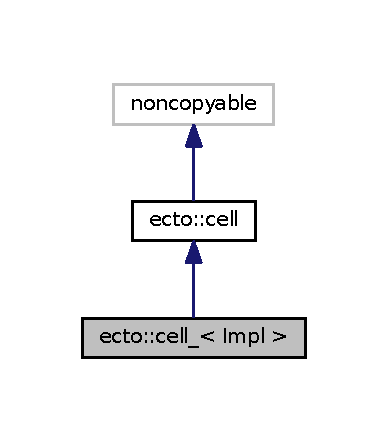
\includegraphics[width=186pt]{structecto_1_1cell____inherit__graph}
\end{center}
\end{figure}


\-Collaboration diagram for ecto\-:\-:cell\-\_\-$<$ \-Impl $>$\-:\nopagebreak
\begin{figure}[H]
\begin{center}
\leavevmode
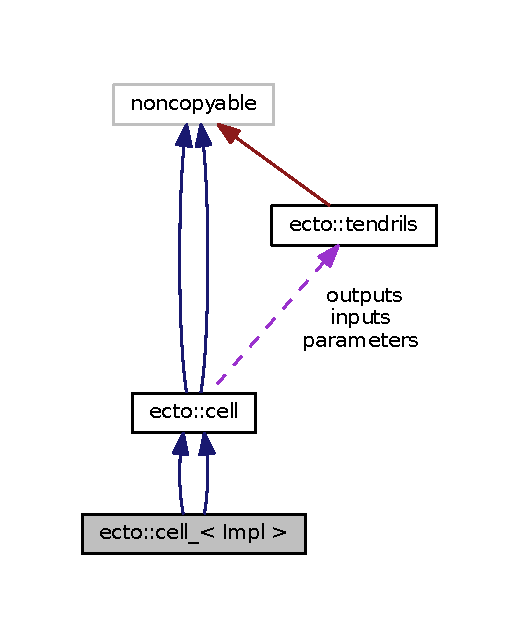
\includegraphics[width=190pt]{structecto_1_1cell____coll__graph}
\end{center}
\end{figure}
\subsection*{\-Classes}
\begin{DoxyCompactItemize}
\item 
struct \hyperlink{structecto_1_1cell___1_1int__}{int\-\_\-}
\end{DoxyCompactItemize}
\subsection*{\-Public \-Types}
\begin{DoxyCompactItemize}
\item 
typedef boost\-::shared\-\_\-ptr\*
$<$ \hyperlink{structecto_1_1cell__}{cell\-\_\-}$<$ \-Impl $>$ $>$ \hyperlink{structecto_1_1cell___a26d9e255a2ba0335c5e90fd04efa6bfa}{ptr}
\begin{DoxyCompactList}\small\item\em \-A convenience pointer typedef. \end{DoxyCompactList}\item 
typedef \hyperlink{structecto_1_1cell___1_1int__}{int\-\_\-}$<$ 0 $>$ \hyperlink{structecto_1_1cell___a3e48e52421d132bb2bb4e343f771abeb}{not\-\_\-implemented}
\item 
typedef \hyperlink{structecto_1_1cell___1_1int__}{int\-\_\-}$<$ 1 $>$ \hyperlink{structecto_1_1cell___a63c5c3dd95630a508017730ee345c23a}{implemented}
\item 
typedef \hyperlink{structecto_1_1cell___1_1int__}{int\-\_\-}$<$ \hyperlink{structecto_1_1has__f}{has\-\_\-f}$<$ \-Impl $>$\*
\-::\hyperlink{structecto_1_1cell___a6a36edc8e9eddadfe6486460bab93c93}{declare\-\_\-params} $>$ \hyperlink{structecto_1_1cell___ab7b111eb2672ae4eaacc668852b8b89f}{has\-\_\-declare\-\_\-params}
\item 
typedef \hyperlink{structecto_1_1cell___1_1int__}{int\-\_\-}$<$ \hyperlink{structecto_1_1has__f}{has\-\_\-f}$<$ \-Impl $>$\*
\-::\hyperlink{structecto_1_1cell___ac08370823fea8ed7f5991e369f6a7fa7}{declare\-\_\-io} $>$ \hyperlink{structecto_1_1cell___a10ab0d3f85e194d548beb3251416a569}{has\-\_\-declare\-\_\-io}
\end{DoxyCompactItemize}
\subsection*{\-Public \-Member \-Functions}
\begin{DoxyCompactItemize}
\item 
\hyperlink{structecto_1_1cell___a8c5059153f9529bf895e3d82f05f5d7e}{cell\-\_\-} ()
\item 
\hyperlink{structecto_1_1cell___a30176d85396dd679e227a272918f422f}{$\sim$cell\-\_\-} ()
\item 
void \hyperlink{structecto_1_1cell___a0e435a14e4cc1d5cd7d80a16f2776565}{dispatch\-\_\-declare\-\_\-params} (\hyperlink{classecto_1_1tendrils}{tendrils} \&params)
\item 
void \hyperlink{structecto_1_1cell___ad95920d295860b791e3fa733fb0745db}{dispatch\-\_\-declare\-\_\-io} (const \hyperlink{classecto_1_1tendrils}{tendrils} \&params, \hyperlink{classecto_1_1tendrils}{tendrils} \&\hyperlink{structecto_1_1cell_a65099b0458a7761b8bfa7a1ddc17e92f}{inputs}, \hyperlink{classecto_1_1tendrils}{tendrils} \&\hyperlink{structecto_1_1cell_a93951743b603faba35312ebdb07ceb22}{outputs})
\item 
void \hyperlink{structecto_1_1cell___a53ab13ad9e8dd9fef55377d85674ff5a}{configure} (const \hyperlink{classecto_1_1tendrils}{tendrils} \&, const \hyperlink{classecto_1_1tendrils}{tendrils} \&, const \hyperlink{classecto_1_1tendrils}{tendrils} \&, \hyperlink{structecto_1_1cell___a3e48e52421d132bb2bb4e343f771abeb}{not\-\_\-implemented})
\item 
void \hyperlink{structecto_1_1cell___acd3caafa6429801f4e121b469bd152a5}{configure} (const \hyperlink{classecto_1_1tendrils}{tendrils} \&params, const \hyperlink{classecto_1_1tendrils}{tendrils} \&\hyperlink{structecto_1_1cell_a65099b0458a7761b8bfa7a1ddc17e92f}{inputs}, const \hyperlink{classecto_1_1tendrils}{tendrils} \&\hyperlink{structecto_1_1cell_a93951743b603faba35312ebdb07ceb22}{outputs}, \hyperlink{structecto_1_1cell___a63c5c3dd95630a508017730ee345c23a}{implemented})
\item 
void \hyperlink{structecto_1_1cell___a953e526cefd3c419a01717740eab9227}{dispatch\-\_\-configure} (const \hyperlink{classecto_1_1tendrils}{tendrils} \&params, const \hyperlink{classecto_1_1tendrils}{tendrils} \&\hyperlink{structecto_1_1cell_a65099b0458a7761b8bfa7a1ddc17e92f}{inputs}, const \hyperlink{classecto_1_1tendrils}{tendrils} \&\hyperlink{structecto_1_1cell_a93951743b603faba35312ebdb07ceb22}{outputs})
\item 
void \hyperlink{structecto_1_1cell___a06dd6747607ad7da98f104bb258fbcbb}{activate} (\hyperlink{structecto_1_1cell___a3e48e52421d132bb2bb4e343f771abeb}{not\-\_\-implemented})
\item 
void \hyperlink{structecto_1_1cell___a8c0319bad42186d2b79a32f7ade1376a}{activate} (\hyperlink{structecto_1_1cell___a63c5c3dd95630a508017730ee345c23a}{implemented})
\item 
void \hyperlink{structecto_1_1cell___a31437fcb5a15e57e8287719f48cecbdd}{dispatch\-\_\-activate} ()
\item 
void \hyperlink{structecto_1_1cell___aa553319fd69477ddf5c2c45cb5c5e3d2}{deactivate} (\hyperlink{structecto_1_1cell___a3e48e52421d132bb2bb4e343f771abeb}{not\-\_\-implemented})
\item 
void \hyperlink{structecto_1_1cell___ab0dc3bd8a6bf42f620a654134df831d3}{deactivate} (\hyperlink{structecto_1_1cell___a63c5c3dd95630a508017730ee345c23a}{implemented})
\item 
void \hyperlink{structecto_1_1cell___a71463eb5e248d29814066904e7f0d515}{dispatch\-\_\-deactivate} ()
\item 
\hyperlink{namespaceecto_a93d82cd28db695d53963fb696582762c}{\-Return\-Code} \hyperlink{structecto_1_1cell___aeb9a98d085805631cc3a3b09c277d5be}{process} (const \hyperlink{classecto_1_1tendrils}{tendrils} \&, const \hyperlink{classecto_1_1tendrils}{tendrils} \&, \hyperlink{structecto_1_1cell___a3e48e52421d132bb2bb4e343f771abeb}{not\-\_\-implemented})
\item 
\hyperlink{namespaceecto_a93d82cd28db695d53963fb696582762c}{\-Return\-Code} \hyperlink{structecto_1_1cell___a310050d75c3a286f013fa16652af6e17}{process} (const \hyperlink{classecto_1_1tendrils}{tendrils} \&\hyperlink{structecto_1_1cell_a65099b0458a7761b8bfa7a1ddc17e92f}{inputs}, const \hyperlink{classecto_1_1tendrils}{tendrils} \&\hyperlink{structecto_1_1cell_a93951743b603faba35312ebdb07ceb22}{outputs}, \hyperlink{structecto_1_1cell___a63c5c3dd95630a508017730ee345c23a}{implemented})
\item 
\hyperlink{namespaceecto_a93d82cd28db695d53963fb696582762c}{\-Return\-Code} \hyperlink{structecto_1_1cell___a1ddd0142b998f0de06a7992c5db27f16}{dispatch\-\_\-process} (const \hyperlink{classecto_1_1tendrils}{tendrils} \&\hyperlink{structecto_1_1cell_a65099b0458a7761b8bfa7a1ddc17e92f}{inputs}, const \hyperlink{classecto_1_1tendrils}{tendrils} \&\hyperlink{structecto_1_1cell_a93951743b603faba35312ebdb07ceb22}{outputs})
\item 
void \hyperlink{structecto_1_1cell___a155401641b4deda52ad3eb8277a9d77d}{start} (\hyperlink{structecto_1_1cell___a3e48e52421d132bb2bb4e343f771abeb}{not\-\_\-implemented})
\item 
void \hyperlink{structecto_1_1cell___afbca5bafc2261f303413fd431f0b12b6}{start} (\hyperlink{structecto_1_1cell___a63c5c3dd95630a508017730ee345c23a}{implemented})
\item 
void \hyperlink{structecto_1_1cell___af6929fe6c16db59235793d972ea20ff8}{dispatch\-\_\-start} ()
\item 
void \hyperlink{structecto_1_1cell___a689e109200f31da6edb491e28b101622}{stop} (\hyperlink{structecto_1_1cell___a3e48e52421d132bb2bb4e343f771abeb}{not\-\_\-implemented})
\item 
void \hyperlink{structecto_1_1cell___ac6da640a23124d5a154884cc6e45531c}{stop} (\hyperlink{structecto_1_1cell___a63c5c3dd95630a508017730ee345c23a}{implemented})
\item 
void \hyperlink{structecto_1_1cell___a0951afcee7f4aa52f957f1a6ecc2bfb7}{dispatch\-\_\-stop} ()
\item 
std\-::string \hyperlink{structecto_1_1cell___a288dac8bba40036b3f3e6b0641833039}{dispatch\-\_\-name} () const 
\item 
std\-::string \hyperlink{structecto_1_1cell___aea843d10de8a002ada9a29bec2ecb815}{dispatch\-\_\-short\-\_\-doc} () const 
\item 
void \hyperlink{structecto_1_1cell___a8d9ca18e234396fcdc1875507d3e11a8}{dispatch\-\_\-short\-\_\-doc} (const std\-::string \&)
\item 
\hyperlink{structecto_1_1cell_af2cab9d2bc012088c4f58c40da57a862}{cell\-::ptr} \hyperlink{structecto_1_1cell___ae2868bb59ddb378cbe7b98fd4e776930}{dispatch\-\_\-clone} () const 
\item 
bool \hyperlink{structecto_1_1cell___a06749143e390dcc5fd90f5076620108c}{init} ()
\item 
\-Impl \& \hyperlink{structecto_1_1cell___a625990e6ac4da1df9be69681881d3e28}{impl} ()
\begin{DoxyCompactList}\small\item\em \-Grab a typed reference to the implementation of the cell. \end{DoxyCompactList}\item 
const \-Impl \& \hyperlink{structecto_1_1cell___a05fe9ed5d606a54f761c104f45994a5e}{impl} () const 
\end{DoxyCompactItemize}
\subsection*{\-Static \-Public \-Member \-Functions}
\begin{DoxyCompactItemize}
\item 
static void \hyperlink{structecto_1_1cell___a6a36edc8e9eddadfe6486460bab93c93}{declare\-\_\-params} (\hyperlink{classecto_1_1tendrils}{tendrils} \&params, \hyperlink{structecto_1_1cell___a3e48e52421d132bb2bb4e343f771abeb}{not\-\_\-implemented})
\item 
static void \hyperlink{structecto_1_1cell___a9673540d6196cfa4e40be503c397b1ac}{declare\-\_\-params} (\hyperlink{classecto_1_1tendrils}{tendrils} \&params, \hyperlink{structecto_1_1cell___a63c5c3dd95630a508017730ee345c23a}{implemented})
\item 
static void \hyperlink{structecto_1_1cell___a4de6c39213d7b583f295c4cb042c1f70}{declare\-\_\-params} (\hyperlink{classecto_1_1tendrils}{tendrils} \&params)
\item 
static void \hyperlink{structecto_1_1cell___ac08370823fea8ed7f5991e369f6a7fa7}{declare\-\_\-io} (const \hyperlink{classecto_1_1tendrils}{tendrils} \&params, \hyperlink{classecto_1_1tendrils}{tendrils} \&\hyperlink{structecto_1_1cell_a65099b0458a7761b8bfa7a1ddc17e92f}{inputs}, \hyperlink{classecto_1_1tendrils}{tendrils} \&\hyperlink{structecto_1_1cell_a93951743b603faba35312ebdb07ceb22}{outputs}, \hyperlink{structecto_1_1cell___a3e48e52421d132bb2bb4e343f771abeb}{not\-\_\-implemented})
\item 
static void \hyperlink{structecto_1_1cell___a20deeac5a09b3a7abaee924f361cbb3b}{declare\-\_\-io} (const \hyperlink{classecto_1_1tendrils}{tendrils} \&params, \hyperlink{classecto_1_1tendrils}{tendrils} \&\hyperlink{structecto_1_1cell_a65099b0458a7761b8bfa7a1ddc17e92f}{inputs}, \hyperlink{classecto_1_1tendrils}{tendrils} \&\hyperlink{structecto_1_1cell_a93951743b603faba35312ebdb07ceb22}{outputs}, \hyperlink{structecto_1_1cell___a63c5c3dd95630a508017730ee345c23a}{implemented})
\item 
static void \hyperlink{structecto_1_1cell___a542f293d31fdd0df4a4414d7b706ef7e}{declare\-\_\-io} (const \hyperlink{classecto_1_1tendrils}{tendrils} \&params, \hyperlink{classecto_1_1tendrils}{tendrils} \&\hyperlink{structecto_1_1cell_a65099b0458a7761b8bfa7a1ddc17e92f}{inputs}, \hyperlink{classecto_1_1tendrils}{tendrils} \&\hyperlink{structecto_1_1cell_a93951743b603faba35312ebdb07ceb22}{outputs})
\end{DoxyCompactItemize}
\subsection*{\-Static \-Public \-Attributes}
\begin{DoxyCompactItemize}
\item 
static std\-::string \hyperlink{structecto_1_1cell___a6a5b6bd083a48acd35ffcf83dacff2f1}{\-S\-H\-O\-R\-T\-\_\-\-D\-O\-C}
\item 
static std\-::string \hyperlink{structecto_1_1cell___aaa9154887542b8d7152f8199e9c6c9bd}{\-C\-E\-L\-L\-\_\-\-N\-A\-M\-E}
\begin{DoxyCompactList}\small\item\em \-The python name for the cell. \end{DoxyCompactList}\item 
static std\-::string \hyperlink{structecto_1_1cell___ab81cf6649132223f620b739a57db04db}{\-M\-O\-D\-U\-L\-E\-\_\-\-N\-A\-M\-E}
\begin{DoxyCompactList}\small\item\em \-The module that the cell is part of. \end{DoxyCompactList}\item 
static const std\-::string \hyperlink{structecto_1_1cell___a26e158738e4e4c8f0ddb64efce30d8d3}{\-C\-E\-L\-L\-\_\-\-T\-Y\-P\-E\-\_\-\-N\-A\-M\-E} = \hyperlink{namespaceecto_a980294f61090496ef65bc6b201f38944}{ecto\-::name\-\_\-of}$<$\-Impl$>$()
\end{DoxyCompactItemize}
\subsection*{\-Private \-Member \-Functions}
\begin{DoxyCompactItemize}
\item 
void \hyperlink{structecto_1_1cell___abb452935616e25bfbb49b77de3f5bcce}{init\-\_\-strand} (boost\-::mpl\-::true\-\_\-)
\item 
void \hyperlink{structecto_1_1cell___a86ac0ef672f44090b0f5e9bf3a8b56dc}{init\-\_\-strand} (boost\-::mpl\-::false\-\_\-)
\end{DoxyCompactItemize}
\subsection*{\-Private \-Attributes}
\begin{DoxyCompactItemize}
\item 
boost\-::scoped\-\_\-ptr$<$ \-Impl $>$ \hyperlink{structecto_1_1cell___a2984b78c1ed24aca6ee427502bd6e8c4}{impl\-\_\-}
\end{DoxyCompactItemize}


\subsection{\-Detailed \-Description}
\subsubsection*{template$<$class Impl$>$struct ecto\-::cell\-\_\-$<$ Impl $>$}

cell\-\_\-$<$\-T$>$ is for registering an arbitrary class with the the cell \-N\-V\-I. \-This adds a barrier between client code and the cell. 

\subsection{\-Member \-Typedef \-Documentation}
\hypertarget{structecto_1_1cell___a10ab0d3f85e194d548beb3251416a569}{\index{ecto\-::cell\-\_\-@{ecto\-::cell\-\_\-}!has\-\_\-declare\-\_\-io@{has\-\_\-declare\-\_\-io}}
\index{has\-\_\-declare\-\_\-io@{has\-\_\-declare\-\_\-io}!ecto::cell_@{ecto\-::cell\-\_\-}}
\subsubsection[{has\-\_\-declare\-\_\-io}]{\setlength{\rightskip}{0pt plus 5cm}template$<$class Impl $>$ typedef {\bf int\-\_\-}$<${\bf has\-\_\-f}$<$\-Impl$>$\-::{\bf declare\-\_\-io}$>$ {\bf ecto\-::cell\-\_\-}$<$ \-Impl $>$\-::{\bf has\-\_\-declare\-\_\-io}}}\label{structecto_1_1cell___a10ab0d3f85e194d548beb3251416a569}
\hypertarget{structecto_1_1cell___ab7b111eb2672ae4eaacc668852b8b89f}{\index{ecto\-::cell\-\_\-@{ecto\-::cell\-\_\-}!has\-\_\-declare\-\_\-params@{has\-\_\-declare\-\_\-params}}
\index{has\-\_\-declare\-\_\-params@{has\-\_\-declare\-\_\-params}!ecto::cell_@{ecto\-::cell\-\_\-}}
\subsubsection[{has\-\_\-declare\-\_\-params}]{\setlength{\rightskip}{0pt plus 5cm}template$<$class Impl $>$ typedef {\bf int\-\_\-}$<${\bf has\-\_\-f}$<$\-Impl$>$\-::{\bf declare\-\_\-params}$>$ {\bf ecto\-::cell\-\_\-}$<$ \-Impl $>$\-::{\bf has\-\_\-declare\-\_\-params}}}\label{structecto_1_1cell___ab7b111eb2672ae4eaacc668852b8b89f}
\hypertarget{structecto_1_1cell___a63c5c3dd95630a508017730ee345c23a}{\index{ecto\-::cell\-\_\-@{ecto\-::cell\-\_\-}!implemented@{implemented}}
\index{implemented@{implemented}!ecto::cell_@{ecto\-::cell\-\_\-}}
\subsubsection[{implemented}]{\setlength{\rightskip}{0pt plus 5cm}template$<$class Impl $>$ typedef {\bf int\-\_\-}$<$1$>$ {\bf ecto\-::cell\-\_\-}$<$ \-Impl $>$\-::{\bf implemented}}}\label{structecto_1_1cell___a63c5c3dd95630a508017730ee345c23a}
\hypertarget{structecto_1_1cell___a3e48e52421d132bb2bb4e343f771abeb}{\index{ecto\-::cell\-\_\-@{ecto\-::cell\-\_\-}!not\-\_\-implemented@{not\-\_\-implemented}}
\index{not\-\_\-implemented@{not\-\_\-implemented}!ecto::cell_@{ecto\-::cell\-\_\-}}
\subsubsection[{not\-\_\-implemented}]{\setlength{\rightskip}{0pt plus 5cm}template$<$class Impl $>$ typedef {\bf int\-\_\-}$<$0$>$ {\bf ecto\-::cell\-\_\-}$<$ \-Impl $>$\-::{\bf not\-\_\-implemented}}}\label{structecto_1_1cell___a3e48e52421d132bb2bb4e343f771abeb}
\hypertarget{structecto_1_1cell___a26d9e255a2ba0335c5e90fd04efa6bfa}{\index{ecto\-::cell\-\_\-@{ecto\-::cell\-\_\-}!ptr@{ptr}}
\index{ptr@{ptr}!ecto::cell_@{ecto\-::cell\-\_\-}}
\subsubsection[{ptr}]{\setlength{\rightskip}{0pt plus 5cm}template$<$class Impl $>$ typedef boost\-::shared\-\_\-ptr$<${\bf cell\-\_\-}$<$\-Impl$>$ $>$ {\bf ecto\-::cell\-\_\-}$<$ \-Impl $>$\-::{\bf ptr}}}\label{structecto_1_1cell___a26d9e255a2ba0335c5e90fd04efa6bfa}


\-A convenience pointer typedef. 



\-Reimplemented from \hyperlink{structecto_1_1cell_af2cab9d2bc012088c4f58c40da57a862}{ecto\-::cell}.



\subsection{\-Constructor \& \-Destructor \-Documentation}
\hypertarget{structecto_1_1cell___a8c5059153f9529bf895e3d82f05f5d7e}{\index{ecto\-::cell\-\_\-@{ecto\-::cell\-\_\-}!cell\-\_\-@{cell\-\_\-}}
\index{cell\-\_\-@{cell\-\_\-}!ecto::cell_@{ecto\-::cell\-\_\-}}
\subsubsection[{cell\-\_\-}]{\setlength{\rightskip}{0pt plus 5cm}template$<$class Impl $>$ {\bf ecto\-::cell\-\_\-}$<$ \-Impl $>$\-::{\bf cell\-\_\-} (
\begin{DoxyParamCaption}
{}
\end{DoxyParamCaption}
)\hspace{0.3cm}{\ttfamily  \mbox{[}inline\mbox{]}}}}\label{structecto_1_1cell___a8c5059153f9529bf895e3d82f05f5d7e}
\hypertarget{structecto_1_1cell___a30176d85396dd679e227a272918f422f}{\index{ecto\-::cell\-\_\-@{ecto\-::cell\-\_\-}!$\sim$cell\-\_\-@{$\sim$cell\-\_\-}}
\index{$\sim$cell\-\_\-@{$\sim$cell\-\_\-}!ecto::cell_@{ecto\-::cell\-\_\-}}
\subsubsection[{$\sim$cell\-\_\-}]{\setlength{\rightskip}{0pt plus 5cm}template$<$class Impl $>$ {\bf ecto\-::cell\-\_\-}$<$ \-Impl $>$\-::$\sim${\bf cell\-\_\-} (
\begin{DoxyParamCaption}
{}
\end{DoxyParamCaption}
)\hspace{0.3cm}{\ttfamily  \mbox{[}inline\mbox{]}}}}\label{structecto_1_1cell___a30176d85396dd679e227a272918f422f}


\subsection{\-Member \-Function \-Documentation}
\hypertarget{structecto_1_1cell___a06dd6747607ad7da98f104bb258fbcbb}{\index{ecto\-::cell\-\_\-@{ecto\-::cell\-\_\-}!activate@{activate}}
\index{activate@{activate}!ecto::cell_@{ecto\-::cell\-\_\-}}
\subsubsection[{activate}]{\setlength{\rightskip}{0pt plus 5cm}template$<$class Impl $>$ void {\bf ecto\-::cell\-\_\-}$<$ \-Impl $>$\-::{\bf activate} (
\begin{DoxyParamCaption}
\item[{{\bf not\-\_\-implemented}}]{}
\end{DoxyParamCaption}
)\hspace{0.3cm}{\ttfamily  \mbox{[}inline\mbox{]}}}}\label{structecto_1_1cell___a06dd6747607ad7da98f104bb258fbcbb}
\hypertarget{structecto_1_1cell___a8c0319bad42186d2b79a32f7ade1376a}{\index{ecto\-::cell\-\_\-@{ecto\-::cell\-\_\-}!activate@{activate}}
\index{activate@{activate}!ecto::cell_@{ecto\-::cell\-\_\-}}
\subsubsection[{activate}]{\setlength{\rightskip}{0pt plus 5cm}template$<$class Impl $>$ void {\bf ecto\-::cell\-\_\-}$<$ \-Impl $>$\-::{\bf activate} (
\begin{DoxyParamCaption}
\item[{{\bf implemented}}]{}
\end{DoxyParamCaption}
)\hspace{0.3cm}{\ttfamily  \mbox{[}inline\mbox{]}}}}\label{structecto_1_1cell___a8c0319bad42186d2b79a32f7ade1376a}
\hypertarget{structecto_1_1cell___a53ab13ad9e8dd9fef55377d85674ff5a}{\index{ecto\-::cell\-\_\-@{ecto\-::cell\-\_\-}!configure@{configure}}
\index{configure@{configure}!ecto::cell_@{ecto\-::cell\-\_\-}}
\subsubsection[{configure}]{\setlength{\rightskip}{0pt plus 5cm}template$<$class Impl $>$ void {\bf ecto\-::cell\-\_\-}$<$ \-Impl $>$\-::{\bf configure} (
\begin{DoxyParamCaption}
\item[{const {\bf tendrils} \&}]{, }
\item[{const {\bf tendrils} \&}]{, }
\item[{const {\bf tendrils} \&}]{, }
\item[{{\bf not\-\_\-implemented}}]{}
\end{DoxyParamCaption}
)\hspace{0.3cm}{\ttfamily  \mbox{[}inline\mbox{]}}}}\label{structecto_1_1cell___a53ab13ad9e8dd9fef55377d85674ff5a}
\hypertarget{structecto_1_1cell___acd3caafa6429801f4e121b469bd152a5}{\index{ecto\-::cell\-\_\-@{ecto\-::cell\-\_\-}!configure@{configure}}
\index{configure@{configure}!ecto::cell_@{ecto\-::cell\-\_\-}}
\subsubsection[{configure}]{\setlength{\rightskip}{0pt plus 5cm}template$<$class Impl $>$ void {\bf ecto\-::cell\-\_\-}$<$ \-Impl $>$\-::{\bf configure} (
\begin{DoxyParamCaption}
\item[{const {\bf tendrils} \&}]{params, }
\item[{const {\bf tendrils} \&}]{inputs, }
\item[{const {\bf tendrils} \&}]{outputs, }
\item[{{\bf implemented}}]{}
\end{DoxyParamCaption}
)\hspace{0.3cm}{\ttfamily  \mbox{[}inline\mbox{]}}}}\label{structecto_1_1cell___acd3caafa6429801f4e121b469bd152a5}
\hypertarget{structecto_1_1cell___aa553319fd69477ddf5c2c45cb5c5e3d2}{\index{ecto\-::cell\-\_\-@{ecto\-::cell\-\_\-}!deactivate@{deactivate}}
\index{deactivate@{deactivate}!ecto::cell_@{ecto\-::cell\-\_\-}}
\subsubsection[{deactivate}]{\setlength{\rightskip}{0pt plus 5cm}template$<$class Impl $>$ void {\bf ecto\-::cell\-\_\-}$<$ \-Impl $>$\-::{\bf deactivate} (
\begin{DoxyParamCaption}
\item[{{\bf not\-\_\-implemented}}]{}
\end{DoxyParamCaption}
)\hspace{0.3cm}{\ttfamily  \mbox{[}inline\mbox{]}}}}\label{structecto_1_1cell___aa553319fd69477ddf5c2c45cb5c5e3d2}
\hypertarget{structecto_1_1cell___ab0dc3bd8a6bf42f620a654134df831d3}{\index{ecto\-::cell\-\_\-@{ecto\-::cell\-\_\-}!deactivate@{deactivate}}
\index{deactivate@{deactivate}!ecto::cell_@{ecto\-::cell\-\_\-}}
\subsubsection[{deactivate}]{\setlength{\rightskip}{0pt plus 5cm}template$<$class Impl $>$ void {\bf ecto\-::cell\-\_\-}$<$ \-Impl $>$\-::{\bf deactivate} (
\begin{DoxyParamCaption}
\item[{{\bf implemented}}]{}
\end{DoxyParamCaption}
)\hspace{0.3cm}{\ttfamily  \mbox{[}inline\mbox{]}}}}\label{structecto_1_1cell___ab0dc3bd8a6bf42f620a654134df831d3}
\hypertarget{structecto_1_1cell___ac08370823fea8ed7f5991e369f6a7fa7}{\index{ecto\-::cell\-\_\-@{ecto\-::cell\-\_\-}!declare\-\_\-io@{declare\-\_\-io}}
\index{declare\-\_\-io@{declare\-\_\-io}!ecto::cell_@{ecto\-::cell\-\_\-}}
\subsubsection[{declare\-\_\-io}]{\setlength{\rightskip}{0pt plus 5cm}template$<$class Impl $>$ static void {\bf ecto\-::cell\-\_\-}$<$ \-Impl $>$\-::{\bf declare\-\_\-io} (
\begin{DoxyParamCaption}
\item[{const {\bf tendrils} \&}]{params, }
\item[{{\bf tendrils} \&}]{inputs, }
\item[{{\bf tendrils} \&}]{outputs, }
\item[{{\bf not\-\_\-implemented}}]{}
\end{DoxyParamCaption}
)\hspace{0.3cm}{\ttfamily  \mbox{[}inline, static\mbox{]}}}}\label{structecto_1_1cell___ac08370823fea8ed7f5991e369f6a7fa7}
\hypertarget{structecto_1_1cell___a20deeac5a09b3a7abaee924f361cbb3b}{\index{ecto\-::cell\-\_\-@{ecto\-::cell\-\_\-}!declare\-\_\-io@{declare\-\_\-io}}
\index{declare\-\_\-io@{declare\-\_\-io}!ecto::cell_@{ecto\-::cell\-\_\-}}
\subsubsection[{declare\-\_\-io}]{\setlength{\rightskip}{0pt plus 5cm}template$<$class Impl $>$ static void {\bf ecto\-::cell\-\_\-}$<$ \-Impl $>$\-::{\bf declare\-\_\-io} (
\begin{DoxyParamCaption}
\item[{const {\bf tendrils} \&}]{params, }
\item[{{\bf tendrils} \&}]{inputs, }
\item[{{\bf tendrils} \&}]{outputs, }
\item[{{\bf implemented}}]{}
\end{DoxyParamCaption}
)\hspace{0.3cm}{\ttfamily  \mbox{[}inline, static\mbox{]}}}}\label{structecto_1_1cell___a20deeac5a09b3a7abaee924f361cbb3b}
\hypertarget{structecto_1_1cell___a542f293d31fdd0df4a4414d7b706ef7e}{\index{ecto\-::cell\-\_\-@{ecto\-::cell\-\_\-}!declare\-\_\-io@{declare\-\_\-io}}
\index{declare\-\_\-io@{declare\-\_\-io}!ecto::cell_@{ecto\-::cell\-\_\-}}
\subsubsection[{declare\-\_\-io}]{\setlength{\rightskip}{0pt plus 5cm}template$<$class Impl $>$ static void {\bf ecto\-::cell\-\_\-}$<$ \-Impl $>$\-::{\bf declare\-\_\-io} (
\begin{DoxyParamCaption}
\item[{const {\bf tendrils} \&}]{params, }
\item[{{\bf tendrils} \&}]{inputs, }
\item[{{\bf tendrils} \&}]{outputs}
\end{DoxyParamCaption}
)\hspace{0.3cm}{\ttfamily  \mbox{[}inline, static\mbox{]}}}}\label{structecto_1_1cell___a542f293d31fdd0df4a4414d7b706ef7e}
\hypertarget{structecto_1_1cell___a6a36edc8e9eddadfe6486460bab93c93}{\index{ecto\-::cell\-\_\-@{ecto\-::cell\-\_\-}!declare\-\_\-params@{declare\-\_\-params}}
\index{declare\-\_\-params@{declare\-\_\-params}!ecto::cell_@{ecto\-::cell\-\_\-}}
\subsubsection[{declare\-\_\-params}]{\setlength{\rightskip}{0pt plus 5cm}template$<$class Impl $>$ static void {\bf ecto\-::cell\-\_\-}$<$ \-Impl $>$\-::{\bf declare\-\_\-params} (
\begin{DoxyParamCaption}
\item[{{\bf tendrils} \&}]{params, }
\item[{{\bf not\-\_\-implemented}}]{}
\end{DoxyParamCaption}
)\hspace{0.3cm}{\ttfamily  \mbox{[}inline, static\mbox{]}}}}\label{structecto_1_1cell___a6a36edc8e9eddadfe6486460bab93c93}
\hypertarget{structecto_1_1cell___a9673540d6196cfa4e40be503c397b1ac}{\index{ecto\-::cell\-\_\-@{ecto\-::cell\-\_\-}!declare\-\_\-params@{declare\-\_\-params}}
\index{declare\-\_\-params@{declare\-\_\-params}!ecto::cell_@{ecto\-::cell\-\_\-}}
\subsubsection[{declare\-\_\-params}]{\setlength{\rightskip}{0pt plus 5cm}template$<$class Impl $>$ static void {\bf ecto\-::cell\-\_\-}$<$ \-Impl $>$\-::{\bf declare\-\_\-params} (
\begin{DoxyParamCaption}
\item[{{\bf tendrils} \&}]{params, }
\item[{{\bf implemented}}]{}
\end{DoxyParamCaption}
)\hspace{0.3cm}{\ttfamily  \mbox{[}inline, static\mbox{]}}}}\label{structecto_1_1cell___a9673540d6196cfa4e40be503c397b1ac}
\hypertarget{structecto_1_1cell___a4de6c39213d7b583f295c4cb042c1f70}{\index{ecto\-::cell\-\_\-@{ecto\-::cell\-\_\-}!declare\-\_\-params@{declare\-\_\-params}}
\index{declare\-\_\-params@{declare\-\_\-params}!ecto::cell_@{ecto\-::cell\-\_\-}}
\subsubsection[{declare\-\_\-params}]{\setlength{\rightskip}{0pt plus 5cm}template$<$class Impl $>$ static void {\bf ecto\-::cell\-\_\-}$<$ \-Impl $>$\-::{\bf declare\-\_\-params} (
\begin{DoxyParamCaption}
\item[{{\bf tendrils} \&}]{params}
\end{DoxyParamCaption}
)\hspace{0.3cm}{\ttfamily  \mbox{[}inline, static\mbox{]}}}}\label{structecto_1_1cell___a4de6c39213d7b583f295c4cb042c1f70}
\hypertarget{structecto_1_1cell___a31437fcb5a15e57e8287719f48cecbdd}{\index{ecto\-::cell\-\_\-@{ecto\-::cell\-\_\-}!dispatch\-\_\-activate@{dispatch\-\_\-activate}}
\index{dispatch\-\_\-activate@{dispatch\-\_\-activate}!ecto::cell_@{ecto\-::cell\-\_\-}}
\subsubsection[{dispatch\-\_\-activate}]{\setlength{\rightskip}{0pt plus 5cm}template$<$class Impl $>$ void {\bf ecto\-::cell\-\_\-}$<$ \-Impl $>$\-::{\bf dispatch\-\_\-activate} (
\begin{DoxyParamCaption}
{}
\end{DoxyParamCaption}
)\hspace{0.3cm}{\ttfamily  \mbox{[}inline, virtual\mbox{]}}}}\label{structecto_1_1cell___a31437fcb5a15e57e8287719f48cecbdd}


\-Implements \hyperlink{structecto_1_1cell_aa345ec700e5e213364c7bb20571cd78d}{ecto\-::cell}.

\hypertarget{structecto_1_1cell___ae2868bb59ddb378cbe7b98fd4e776930}{\index{ecto\-::cell\-\_\-@{ecto\-::cell\-\_\-}!dispatch\-\_\-clone@{dispatch\-\_\-clone}}
\index{dispatch\-\_\-clone@{dispatch\-\_\-clone}!ecto::cell_@{ecto\-::cell\-\_\-}}
\subsubsection[{dispatch\-\_\-clone}]{\setlength{\rightskip}{0pt plus 5cm}template$<$class Impl $>$ {\bf cell\-::ptr} {\bf ecto\-::cell\-\_\-}$<$ \-Impl $>$\-::{\bf dispatch\-\_\-clone} (
\begin{DoxyParamCaption}
{}
\end{DoxyParamCaption}
) const\hspace{0.3cm}{\ttfamily  \mbox{[}inline, virtual\mbox{]}}}}\label{structecto_1_1cell___ae2868bb59ddb378cbe7b98fd4e776930}


\-Implements \hyperlink{structecto_1_1cell_a7beccd749c33bd8b4c5827598e8fe5a5}{ecto\-::cell}.

\hypertarget{structecto_1_1cell___a953e526cefd3c419a01717740eab9227}{\index{ecto\-::cell\-\_\-@{ecto\-::cell\-\_\-}!dispatch\-\_\-configure@{dispatch\-\_\-configure}}
\index{dispatch\-\_\-configure@{dispatch\-\_\-configure}!ecto::cell_@{ecto\-::cell\-\_\-}}
\subsubsection[{dispatch\-\_\-configure}]{\setlength{\rightskip}{0pt plus 5cm}template$<$class Impl $>$ void {\bf ecto\-::cell\-\_\-}$<$ \-Impl $>$\-::{\bf dispatch\-\_\-configure} (
\begin{DoxyParamCaption}
\item[{const {\bf tendrils} \&}]{params, }
\item[{const {\bf tendrils} \&}]{inputs, }
\item[{const {\bf tendrils} \&}]{outputs}
\end{DoxyParamCaption}
)\hspace{0.3cm}{\ttfamily  \mbox{[}inline, virtual\mbox{]}}}}\label{structecto_1_1cell___a953e526cefd3c419a01717740eab9227}


\-Implements \hyperlink{structecto_1_1cell_a19c7c679dededd37ace918bf0ff31cd3}{ecto\-::cell}.

\hypertarget{structecto_1_1cell___a71463eb5e248d29814066904e7f0d515}{\index{ecto\-::cell\-\_\-@{ecto\-::cell\-\_\-}!dispatch\-\_\-deactivate@{dispatch\-\_\-deactivate}}
\index{dispatch\-\_\-deactivate@{dispatch\-\_\-deactivate}!ecto::cell_@{ecto\-::cell\-\_\-}}
\subsubsection[{dispatch\-\_\-deactivate}]{\setlength{\rightskip}{0pt plus 5cm}template$<$class Impl $>$ void {\bf ecto\-::cell\-\_\-}$<$ \-Impl $>$\-::{\bf dispatch\-\_\-deactivate} (
\begin{DoxyParamCaption}
{}
\end{DoxyParamCaption}
)\hspace{0.3cm}{\ttfamily  \mbox{[}inline, virtual\mbox{]}}}}\label{structecto_1_1cell___a71463eb5e248d29814066904e7f0d515}


\-Implements \hyperlink{structecto_1_1cell_a4b5f111fc7b90dccce0cd70e28c9be62}{ecto\-::cell}.

\hypertarget{structecto_1_1cell___ad95920d295860b791e3fa733fb0745db}{\index{ecto\-::cell\-\_\-@{ecto\-::cell\-\_\-}!dispatch\-\_\-declare\-\_\-io@{dispatch\-\_\-declare\-\_\-io}}
\index{dispatch\-\_\-declare\-\_\-io@{dispatch\-\_\-declare\-\_\-io}!ecto::cell_@{ecto\-::cell\-\_\-}}
\subsubsection[{dispatch\-\_\-declare\-\_\-io}]{\setlength{\rightskip}{0pt plus 5cm}template$<$class Impl $>$ void {\bf ecto\-::cell\-\_\-}$<$ \-Impl $>$\-::{\bf dispatch\-\_\-declare\-\_\-io} (
\begin{DoxyParamCaption}
\item[{const {\bf tendrils} \&}]{params, }
\item[{{\bf tendrils} \&}]{inputs, }
\item[{{\bf tendrils} \&}]{outputs}
\end{DoxyParamCaption}
)\hspace{0.3cm}{\ttfamily  \mbox{[}inline, virtual\mbox{]}}}}\label{structecto_1_1cell___ad95920d295860b791e3fa733fb0745db}


\-Implements \hyperlink{structecto_1_1cell_acb4cdb70f2db329ba9c615d74c63a4b2}{ecto\-::cell}.

\hypertarget{structecto_1_1cell___a0e435a14e4cc1d5cd7d80a16f2776565}{\index{ecto\-::cell\-\_\-@{ecto\-::cell\-\_\-}!dispatch\-\_\-declare\-\_\-params@{dispatch\-\_\-declare\-\_\-params}}
\index{dispatch\-\_\-declare\-\_\-params@{dispatch\-\_\-declare\-\_\-params}!ecto::cell_@{ecto\-::cell\-\_\-}}
\subsubsection[{dispatch\-\_\-declare\-\_\-params}]{\setlength{\rightskip}{0pt plus 5cm}template$<$class Impl $>$ void {\bf ecto\-::cell\-\_\-}$<$ \-Impl $>$\-::{\bf dispatch\-\_\-declare\-\_\-params} (
\begin{DoxyParamCaption}
\item[{{\bf tendrils} \&}]{params}
\end{DoxyParamCaption}
)\hspace{0.3cm}{\ttfamily  \mbox{[}inline, virtual\mbox{]}}}}\label{structecto_1_1cell___a0e435a14e4cc1d5cd7d80a16f2776565}


\-Implements \hyperlink{structecto_1_1cell_abcf3cc29703214a7ede63d652e17ee96}{ecto\-::cell}.

\hypertarget{structecto_1_1cell___a288dac8bba40036b3f3e6b0641833039}{\index{ecto\-::cell\-\_\-@{ecto\-::cell\-\_\-}!dispatch\-\_\-name@{dispatch\-\_\-name}}
\index{dispatch\-\_\-name@{dispatch\-\_\-name}!ecto::cell_@{ecto\-::cell\-\_\-}}
\subsubsection[{dispatch\-\_\-name}]{\setlength{\rightskip}{0pt plus 5cm}template$<$class Impl $>$ std\-::string {\bf ecto\-::cell\-\_\-}$<$ \-Impl $>$\-::{\bf dispatch\-\_\-name} (
\begin{DoxyParamCaption}
{}
\end{DoxyParamCaption}
) const\hspace{0.3cm}{\ttfamily  \mbox{[}inline, virtual\mbox{]}}}}\label{structecto_1_1cell___a288dac8bba40036b3f3e6b0641833039}


\-Implements \hyperlink{structecto_1_1cell_a456b56e3291f5e2bb68ce31a4a43ece5}{ecto\-::cell}.

\hypertarget{structecto_1_1cell___a1ddd0142b998f0de06a7992c5db27f16}{\index{ecto\-::cell\-\_\-@{ecto\-::cell\-\_\-}!dispatch\-\_\-process@{dispatch\-\_\-process}}
\index{dispatch\-\_\-process@{dispatch\-\_\-process}!ecto::cell_@{ecto\-::cell\-\_\-}}
\subsubsection[{dispatch\-\_\-process}]{\setlength{\rightskip}{0pt plus 5cm}template$<$class Impl $>$ {\bf \-Return\-Code} {\bf ecto\-::cell\-\_\-}$<$ \-Impl $>$\-::{\bf dispatch\-\_\-process} (
\begin{DoxyParamCaption}
\item[{const {\bf tendrils} \&}]{inputs, }
\item[{const {\bf tendrils} \&}]{outputs}
\end{DoxyParamCaption}
)\hspace{0.3cm}{\ttfamily  \mbox{[}inline, virtual\mbox{]}}}}\label{structecto_1_1cell___a1ddd0142b998f0de06a7992c5db27f16}


\-Implements \hyperlink{structecto_1_1cell_a390bd83cfdff120523efc5c3e76bc3e5}{ecto\-::cell}.

\hypertarget{structecto_1_1cell___aea843d10de8a002ada9a29bec2ecb815}{\index{ecto\-::cell\-\_\-@{ecto\-::cell\-\_\-}!dispatch\-\_\-short\-\_\-doc@{dispatch\-\_\-short\-\_\-doc}}
\index{dispatch\-\_\-short\-\_\-doc@{dispatch\-\_\-short\-\_\-doc}!ecto::cell_@{ecto\-::cell\-\_\-}}
\subsubsection[{dispatch\-\_\-short\-\_\-doc}]{\setlength{\rightskip}{0pt plus 5cm}template$<$class Impl $>$ std\-::string {\bf ecto\-::cell\-\_\-}$<$ \-Impl $>$\-::{\bf dispatch\-\_\-short\-\_\-doc} (
\begin{DoxyParamCaption}
{}
\end{DoxyParamCaption}
) const\hspace{0.3cm}{\ttfamily  \mbox{[}inline, virtual\mbox{]}}}}\label{structecto_1_1cell___aea843d10de8a002ada9a29bec2ecb815}


\-Reimplemented from \hyperlink{structecto_1_1cell_a400b8aecf15588cfb21d712fbb000e8a}{ecto\-::cell}.

\hypertarget{structecto_1_1cell___a8d9ca18e234396fcdc1875507d3e11a8}{\index{ecto\-::cell\-\_\-@{ecto\-::cell\-\_\-}!dispatch\-\_\-short\-\_\-doc@{dispatch\-\_\-short\-\_\-doc}}
\index{dispatch\-\_\-short\-\_\-doc@{dispatch\-\_\-short\-\_\-doc}!ecto::cell_@{ecto\-::cell\-\_\-}}
\subsubsection[{dispatch\-\_\-short\-\_\-doc}]{\setlength{\rightskip}{0pt plus 5cm}template$<$class Impl $>$ void {\bf ecto\-::cell\-\_\-}$<$ \-Impl $>$\-::{\bf dispatch\-\_\-short\-\_\-doc} (
\begin{DoxyParamCaption}
\item[{const std\-::string \&}]{}
\end{DoxyParamCaption}
)\hspace{0.3cm}{\ttfamily  \mbox{[}inline, virtual\mbox{]}}}}\label{structecto_1_1cell___a8d9ca18e234396fcdc1875507d3e11a8}


\-Reimplemented from \hyperlink{structecto_1_1cell_a407d24db843ffe12ac57c9a8827a9fe8}{ecto\-::cell}.

\hypertarget{structecto_1_1cell___af6929fe6c16db59235793d972ea20ff8}{\index{ecto\-::cell\-\_\-@{ecto\-::cell\-\_\-}!dispatch\-\_\-start@{dispatch\-\_\-start}}
\index{dispatch\-\_\-start@{dispatch\-\_\-start}!ecto::cell_@{ecto\-::cell\-\_\-}}
\subsubsection[{dispatch\-\_\-start}]{\setlength{\rightskip}{0pt plus 5cm}template$<$class Impl $>$ void {\bf ecto\-::cell\-\_\-}$<$ \-Impl $>$\-::{\bf dispatch\-\_\-start} (
\begin{DoxyParamCaption}
{}
\end{DoxyParamCaption}
)\hspace{0.3cm}{\ttfamily  \mbox{[}inline, virtual\mbox{]}}}}\label{structecto_1_1cell___af6929fe6c16db59235793d972ea20ff8}


\-Implements \hyperlink{structecto_1_1cell_ab5c75358dd32fa811116654bdc76385b}{ecto\-::cell}.

\hypertarget{structecto_1_1cell___a0951afcee7f4aa52f957f1a6ecc2bfb7}{\index{ecto\-::cell\-\_\-@{ecto\-::cell\-\_\-}!dispatch\-\_\-stop@{dispatch\-\_\-stop}}
\index{dispatch\-\_\-stop@{dispatch\-\_\-stop}!ecto::cell_@{ecto\-::cell\-\_\-}}
\subsubsection[{dispatch\-\_\-stop}]{\setlength{\rightskip}{0pt plus 5cm}template$<$class Impl $>$ void {\bf ecto\-::cell\-\_\-}$<$ \-Impl $>$\-::{\bf dispatch\-\_\-stop} (
\begin{DoxyParamCaption}
{}
\end{DoxyParamCaption}
)\hspace{0.3cm}{\ttfamily  \mbox{[}inline, virtual\mbox{]}}}}\label{structecto_1_1cell___a0951afcee7f4aa52f957f1a6ecc2bfb7}


\-Implements \hyperlink{structecto_1_1cell_a65ff7141e927a7115a785478a03b94bc}{ecto\-::cell}.

\hypertarget{structecto_1_1cell___a625990e6ac4da1df9be69681881d3e28}{\index{ecto\-::cell\-\_\-@{ecto\-::cell\-\_\-}!impl@{impl}}
\index{impl@{impl}!ecto::cell_@{ecto\-::cell\-\_\-}}
\subsubsection[{impl}]{\setlength{\rightskip}{0pt plus 5cm}template$<$class Impl $>$ \-Impl\& {\bf ecto\-::cell\-\_\-}$<$ \-Impl $>$\-::{\bf impl} (
\begin{DoxyParamCaption}
{}
\end{DoxyParamCaption}
)\hspace{0.3cm}{\ttfamily  \mbox{[}inline\mbox{]}}}}\label{structecto_1_1cell___a625990e6ac4da1df9be69681881d3e28}


\-Grab a typed reference to the implementation of the cell. 

\hypertarget{structecto_1_1cell___a05fe9ed5d606a54f761c104f45994a5e}{\index{ecto\-::cell\-\_\-@{ecto\-::cell\-\_\-}!impl@{impl}}
\index{impl@{impl}!ecto::cell_@{ecto\-::cell\-\_\-}}
\subsubsection[{impl}]{\setlength{\rightskip}{0pt plus 5cm}template$<$class Impl $>$ const \-Impl\& {\bf ecto\-::cell\-\_\-}$<$ \-Impl $>$\-::{\bf impl} (
\begin{DoxyParamCaption}
{}
\end{DoxyParamCaption}
) const\hspace{0.3cm}{\ttfamily  \mbox{[}inline\mbox{]}}}}\label{structecto_1_1cell___a05fe9ed5d606a54f761c104f45994a5e}
\hypertarget{structecto_1_1cell___a06749143e390dcc5fd90f5076620108c}{\index{ecto\-::cell\-\_\-@{ecto\-::cell\-\_\-}!init@{init}}
\index{init@{init}!ecto::cell_@{ecto\-::cell\-\_\-}}
\subsubsection[{init}]{\setlength{\rightskip}{0pt plus 5cm}template$<$typename Impl $>$ bool {\bf ecto\-::cell\-\_\-}$<$ \-Impl $>$\-::{\bf init} (
\begin{DoxyParamCaption}
{}
\end{DoxyParamCaption}
)\hspace{0.3cm}{\ttfamily  \mbox{[}virtual\mbox{]}}}}\label{structecto_1_1cell___a06749143e390dcc5fd90f5076620108c}


\-Implements \hyperlink{structecto_1_1cell_ab9a6c3fd8f76289f338a9e05368b1aff}{ecto\-::cell}.

\hypertarget{structecto_1_1cell___abb452935616e25bfbb49b77de3f5bcce}{\index{ecto\-::cell\-\_\-@{ecto\-::cell\-\_\-}!init\-\_\-strand@{init\-\_\-strand}}
\index{init\-\_\-strand@{init\-\_\-strand}!ecto::cell_@{ecto\-::cell\-\_\-}}
\subsubsection[{init\-\_\-strand}]{\setlength{\rightskip}{0pt plus 5cm}template$<$class Impl $>$ void {\bf ecto\-::cell\-\_\-}$<$ \-Impl $>$\-::{\bf init\-\_\-strand} (
\begin{DoxyParamCaption}
\item[{boost\-::mpl\-::true\-\_\-}]{}
\end{DoxyParamCaption}
)\hspace{0.3cm}{\ttfamily  \mbox{[}inline, private\mbox{]}}}}\label{structecto_1_1cell___abb452935616e25bfbb49b77de3f5bcce}
\hypertarget{structecto_1_1cell___a86ac0ef672f44090b0f5e9bf3a8b56dc}{\index{ecto\-::cell\-\_\-@{ecto\-::cell\-\_\-}!init\-\_\-strand@{init\-\_\-strand}}
\index{init\-\_\-strand@{init\-\_\-strand}!ecto::cell_@{ecto\-::cell\-\_\-}}
\subsubsection[{init\-\_\-strand}]{\setlength{\rightskip}{0pt plus 5cm}template$<$class Impl $>$ void {\bf ecto\-::cell\-\_\-}$<$ \-Impl $>$\-::{\bf init\-\_\-strand} (
\begin{DoxyParamCaption}
\item[{boost\-::mpl\-::false\-\_\-}]{}
\end{DoxyParamCaption}
)\hspace{0.3cm}{\ttfamily  \mbox{[}inline, private\mbox{]}}}}\label{structecto_1_1cell___a86ac0ef672f44090b0f5e9bf3a8b56dc}
\hypertarget{structecto_1_1cell___aeb9a98d085805631cc3a3b09c277d5be}{\index{ecto\-::cell\-\_\-@{ecto\-::cell\-\_\-}!process@{process}}
\index{process@{process}!ecto::cell_@{ecto\-::cell\-\_\-}}
\subsubsection[{process}]{\setlength{\rightskip}{0pt plus 5cm}template$<$class Impl $>$ {\bf \-Return\-Code} {\bf ecto\-::cell\-\_\-}$<$ \-Impl $>$\-::{\bf process} (
\begin{DoxyParamCaption}
\item[{const {\bf tendrils} \&}]{, }
\item[{const {\bf tendrils} \&}]{, }
\item[{{\bf not\-\_\-implemented}}]{}
\end{DoxyParamCaption}
)\hspace{0.3cm}{\ttfamily  \mbox{[}inline\mbox{]}}}}\label{structecto_1_1cell___aeb9a98d085805631cc3a3b09c277d5be}
\hypertarget{structecto_1_1cell___a310050d75c3a286f013fa16652af6e17}{\index{ecto\-::cell\-\_\-@{ecto\-::cell\-\_\-}!process@{process}}
\index{process@{process}!ecto::cell_@{ecto\-::cell\-\_\-}}
\subsubsection[{process}]{\setlength{\rightskip}{0pt plus 5cm}template$<$class Impl $>$ {\bf \-Return\-Code} {\bf ecto\-::cell\-\_\-}$<$ \-Impl $>$\-::{\bf process} (
\begin{DoxyParamCaption}
\item[{const {\bf tendrils} \&}]{inputs, }
\item[{const {\bf tendrils} \&}]{outputs, }
\item[{{\bf implemented}}]{}
\end{DoxyParamCaption}
)\hspace{0.3cm}{\ttfamily  \mbox{[}inline\mbox{]}}}}\label{structecto_1_1cell___a310050d75c3a286f013fa16652af6e17}
\hypertarget{structecto_1_1cell___a155401641b4deda52ad3eb8277a9d77d}{\index{ecto\-::cell\-\_\-@{ecto\-::cell\-\_\-}!start@{start}}
\index{start@{start}!ecto::cell_@{ecto\-::cell\-\_\-}}
\subsubsection[{start}]{\setlength{\rightskip}{0pt plus 5cm}template$<$class Impl $>$ void {\bf ecto\-::cell\-\_\-}$<$ \-Impl $>$\-::{\bf start} (
\begin{DoxyParamCaption}
\item[{{\bf not\-\_\-implemented}}]{}
\end{DoxyParamCaption}
)\hspace{0.3cm}{\ttfamily  \mbox{[}inline\mbox{]}}}}\label{structecto_1_1cell___a155401641b4deda52ad3eb8277a9d77d}
\hypertarget{structecto_1_1cell___afbca5bafc2261f303413fd431f0b12b6}{\index{ecto\-::cell\-\_\-@{ecto\-::cell\-\_\-}!start@{start}}
\index{start@{start}!ecto::cell_@{ecto\-::cell\-\_\-}}
\subsubsection[{start}]{\setlength{\rightskip}{0pt plus 5cm}template$<$class Impl $>$ void {\bf ecto\-::cell\-\_\-}$<$ \-Impl $>$\-::{\bf start} (
\begin{DoxyParamCaption}
\item[{{\bf implemented}}]{}
\end{DoxyParamCaption}
)\hspace{0.3cm}{\ttfamily  \mbox{[}inline\mbox{]}}}}\label{structecto_1_1cell___afbca5bafc2261f303413fd431f0b12b6}
\hypertarget{structecto_1_1cell___a689e109200f31da6edb491e28b101622}{\index{ecto\-::cell\-\_\-@{ecto\-::cell\-\_\-}!stop@{stop}}
\index{stop@{stop}!ecto::cell_@{ecto\-::cell\-\_\-}}
\subsubsection[{stop}]{\setlength{\rightskip}{0pt plus 5cm}template$<$class Impl $>$ void {\bf ecto\-::cell\-\_\-}$<$ \-Impl $>$\-::{\bf stop} (
\begin{DoxyParamCaption}
\item[{{\bf not\-\_\-implemented}}]{}
\end{DoxyParamCaption}
)\hspace{0.3cm}{\ttfamily  \mbox{[}inline\mbox{]}}}}\label{structecto_1_1cell___a689e109200f31da6edb491e28b101622}
\hypertarget{structecto_1_1cell___ac6da640a23124d5a154884cc6e45531c}{\index{ecto\-::cell\-\_\-@{ecto\-::cell\-\_\-}!stop@{stop}}
\index{stop@{stop}!ecto::cell_@{ecto\-::cell\-\_\-}}
\subsubsection[{stop}]{\setlength{\rightskip}{0pt plus 5cm}template$<$class Impl $>$ void {\bf ecto\-::cell\-\_\-}$<$ \-Impl $>$\-::{\bf stop} (
\begin{DoxyParamCaption}
\item[{{\bf implemented}}]{}
\end{DoxyParamCaption}
)\hspace{0.3cm}{\ttfamily  \mbox{[}inline\mbox{]}}}}\label{structecto_1_1cell___ac6da640a23124d5a154884cc6e45531c}


\subsection{\-Member \-Data \-Documentation}
\hypertarget{structecto_1_1cell___aaa9154887542b8d7152f8199e9c6c9bd}{\index{ecto\-::cell\-\_\-@{ecto\-::cell\-\_\-}!\-C\-E\-L\-L\-\_\-\-N\-A\-M\-E@{\-C\-E\-L\-L\-\_\-\-N\-A\-M\-E}}
\index{\-C\-E\-L\-L\-\_\-\-N\-A\-M\-E@{\-C\-E\-L\-L\-\_\-\-N\-A\-M\-E}!ecto::cell_@{ecto\-::cell\-\_\-}}
\subsubsection[{\-C\-E\-L\-L\-\_\-\-N\-A\-M\-E}]{\setlength{\rightskip}{0pt plus 5cm}template$<$class Impl $>$ std\-::string {\bf ecto\-::cell\-\_\-}$<$ \-Impl $>$\-::{\bf \-C\-E\-L\-L\-\_\-\-N\-A\-M\-E}\hspace{0.3cm}{\ttfamily  \mbox{[}static\mbox{]}}}}\label{structecto_1_1cell___aaa9154887542b8d7152f8199e9c6c9bd}


\-The python name for the cell. 

\hypertarget{structecto_1_1cell___a26e158738e4e4c8f0ddb64efce30d8d3}{\index{ecto\-::cell\-\_\-@{ecto\-::cell\-\_\-}!\-C\-E\-L\-L\-\_\-\-T\-Y\-P\-E\-\_\-\-N\-A\-M\-E@{\-C\-E\-L\-L\-\_\-\-T\-Y\-P\-E\-\_\-\-N\-A\-M\-E}}
\index{\-C\-E\-L\-L\-\_\-\-T\-Y\-P\-E\-\_\-\-N\-A\-M\-E@{\-C\-E\-L\-L\-\_\-\-T\-Y\-P\-E\-\_\-\-N\-A\-M\-E}!ecto::cell_@{ecto\-::cell\-\_\-}}
\subsubsection[{\-C\-E\-L\-L\-\_\-\-T\-Y\-P\-E\-\_\-\-N\-A\-M\-E}]{\setlength{\rightskip}{0pt plus 5cm}template$<$class Impl $>$ const std\-::string {\bf ecto\-::cell\-\_\-}$<$ \-Impl $>$\-::{\bf \-C\-E\-L\-L\-\_\-\-T\-Y\-P\-E\-\_\-\-N\-A\-M\-E} = {\bf ecto\-::name\-\_\-of}$<$\-Impl$>$()\hspace{0.3cm}{\ttfamily  \mbox{[}static\mbox{]}}}}\label{structecto_1_1cell___a26e158738e4e4c8f0ddb64efce30d8d3}
\hypertarget{structecto_1_1cell___a2984b78c1ed24aca6ee427502bd6e8c4}{\index{ecto\-::cell\-\_\-@{ecto\-::cell\-\_\-}!impl\-\_\-@{impl\-\_\-}}
\index{impl\-\_\-@{impl\-\_\-}!ecto::cell_@{ecto\-::cell\-\_\-}}
\subsubsection[{impl\-\_\-}]{\setlength{\rightskip}{0pt plus 5cm}template$<$class Impl $>$ boost\-::scoped\-\_\-ptr$<$\-Impl$>$ {\bf ecto\-::cell\-\_\-}$<$ \-Impl $>$\-::{\bf impl\-\_\-}\hspace{0.3cm}{\ttfamily  \mbox{[}private\mbox{]}}}}\label{structecto_1_1cell___a2984b78c1ed24aca6ee427502bd6e8c4}
\hypertarget{structecto_1_1cell___ab81cf6649132223f620b739a57db04db}{\index{ecto\-::cell\-\_\-@{ecto\-::cell\-\_\-}!\-M\-O\-D\-U\-L\-E\-\_\-\-N\-A\-M\-E@{\-M\-O\-D\-U\-L\-E\-\_\-\-N\-A\-M\-E}}
\index{\-M\-O\-D\-U\-L\-E\-\_\-\-N\-A\-M\-E@{\-M\-O\-D\-U\-L\-E\-\_\-\-N\-A\-M\-E}!ecto::cell_@{ecto\-::cell\-\_\-}}
\subsubsection[{\-M\-O\-D\-U\-L\-E\-\_\-\-N\-A\-M\-E}]{\setlength{\rightskip}{0pt plus 5cm}template$<$class Impl $>$ std\-::string {\bf ecto\-::cell\-\_\-}$<$ \-Impl $>$\-::{\bf \-M\-O\-D\-U\-L\-E\-\_\-\-N\-A\-M\-E}\hspace{0.3cm}{\ttfamily  \mbox{[}static\mbox{]}}}}\label{structecto_1_1cell___ab81cf6649132223f620b739a57db04db}


\-The module that the cell is part of. 

\hypertarget{structecto_1_1cell___a6a5b6bd083a48acd35ffcf83dacff2f1}{\index{ecto\-::cell\-\_\-@{ecto\-::cell\-\_\-}!\-S\-H\-O\-R\-T\-\_\-\-D\-O\-C@{\-S\-H\-O\-R\-T\-\_\-\-D\-O\-C}}
\index{\-S\-H\-O\-R\-T\-\_\-\-D\-O\-C@{\-S\-H\-O\-R\-T\-\_\-\-D\-O\-C}!ecto::cell_@{ecto\-::cell\-\_\-}}
\subsubsection[{\-S\-H\-O\-R\-T\-\_\-\-D\-O\-C}]{\setlength{\rightskip}{0pt plus 5cm}template$<$class Impl $>$ std\-::string {\bf ecto\-::cell\-\_\-}$<$ \-Impl $>$\-::{\bf \-S\-H\-O\-R\-T\-\_\-\-D\-O\-C}\hspace{0.3cm}{\ttfamily  \mbox{[}static\mbox{]}}}}\label{structecto_1_1cell___a6a5b6bd083a48acd35ffcf83dacff2f1}


\-The documentation for this struct was generated from the following file\-:\begin{DoxyCompactItemize}
\item 
/home/vrabaud/workspace/recognition\-\_\-kitchen\-\_\-groovy/src/ecto/include/ecto/\hyperlink{cell_8hpp}{cell.\-hpp}\end{DoxyCompactItemize}

\hypertarget{structecto_1_1tendril_1_1Converter}{\section{ecto\-:\-:tendril\-:\-:Converter Struct Reference}
\label{structecto_1_1tendril_1_1Converter}\index{ecto\-::tendril\-::\-Converter@{ecto\-::tendril\-::\-Converter}}
}


Inheritance diagram for ecto\-:\-:tendril\-:\-:Converter\-:\nopagebreak
\begin{figure}[H]
\begin{center}
\leavevmode
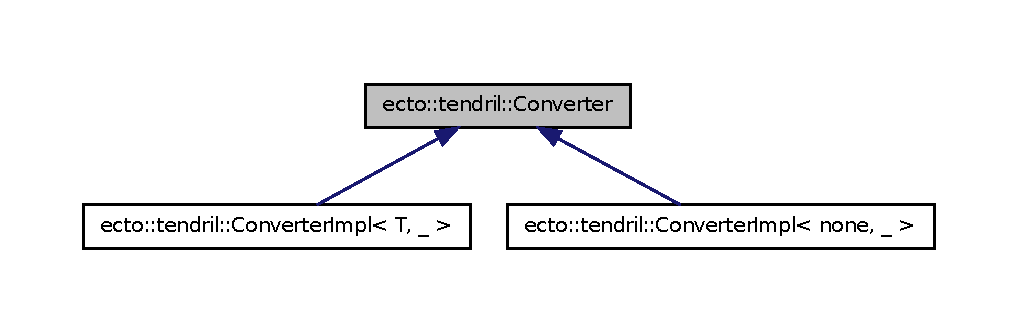
\includegraphics[width=350pt]{structecto_1_1tendril_1_1Converter__inherit__graph}
\end{center}
\end{figure}
\subsection*{Public Member Functions}
\begin{DoxyCompactItemize}
\item 
virtual void \hyperlink{structecto_1_1tendril_1_1Converter_a9987df3be3c0657bea97eeeaa190e48a}{operator()} (\hyperlink{classecto_1_1tendril}{tendril} \&t, const boost\-::python\-::object \&o) const =0
\item 
virtual void \hyperlink{structecto_1_1tendril_1_1Converter_a73562ca297e0c5d1c6fef136701f50d3}{operator()} (boost\-::python\-::object \&o, const \hyperlink{classecto_1_1tendril}{tendril} \&t) const =0
\end{DoxyCompactItemize}


\subsection{Member Function Documentation}
\hypertarget{structecto_1_1tendril_1_1Converter_a9987df3be3c0657bea97eeeaa190e48a}{\index{ecto\-::tendril\-::\-Converter@{ecto\-::tendril\-::\-Converter}!operator()@{operator()}}
\index{operator()@{operator()}!ecto::tendril::Converter@{ecto\-::tendril\-::\-Converter}}
\subsubsection[{operator()}]{\setlength{\rightskip}{0pt plus 5cm}virtual void ecto\-::tendril\-::\-Converter\-::operator() (
\begin{DoxyParamCaption}
\item[{{\bf tendril} \&}]{t, }
\item[{const boost\-::python\-::object \&}]{o}
\end{DoxyParamCaption}
) const\hspace{0.3cm}{\ttfamily [pure virtual]}}}\label{structecto_1_1tendril_1_1Converter_a9987df3be3c0657bea97eeeaa190e48a}


Implemented in \hyperlink{structecto_1_1tendril_1_1ConverterImpl_3_01none_00_01___01_4_ac139edd43cc2f8371eee89ed029166d4}{ecto\-::tendril\-::\-Converter\-Impl$<$ none, \-\_\- $>$}, \hyperlink{structecto_1_1tendril_1_1ConverterImpl_aa03b80197057d2810198e3029a150988}{ecto\-::tendril\-::\-Converter\-Impl$<$ T, \-\_\- $>$}, and \hyperlink{structecto_1_1tendril_1_1ConverterImpl_aa03b80197057d2810198e3029a150988}{ecto\-::tendril\-::\-Converter\-Impl$<$ ecto\-::tendril\-::none, \-\_\- $>$}.

\hypertarget{structecto_1_1tendril_1_1Converter_a73562ca297e0c5d1c6fef136701f50d3}{\index{ecto\-::tendril\-::\-Converter@{ecto\-::tendril\-::\-Converter}!operator()@{operator()}}
\index{operator()@{operator()}!ecto::tendril::Converter@{ecto\-::tendril\-::\-Converter}}
\subsubsection[{operator()}]{\setlength{\rightskip}{0pt plus 5cm}virtual void ecto\-::tendril\-::\-Converter\-::operator() (
\begin{DoxyParamCaption}
\item[{boost\-::python\-::object \&}]{o, }
\item[{const {\bf tendril} \&}]{t}
\end{DoxyParamCaption}
) const\hspace{0.3cm}{\ttfamily [pure virtual]}}}\label{structecto_1_1tendril_1_1Converter_a73562ca297e0c5d1c6fef136701f50d3}


Implemented in \hyperlink{structecto_1_1tendril_1_1ConverterImpl_3_01none_00_01___01_4_afbc6677e2eacb4352bff1b6f2aa94eee}{ecto\-::tendril\-::\-Converter\-Impl$<$ none, \-\_\- $>$}, \hyperlink{structecto_1_1tendril_1_1ConverterImpl_a1b9b248c9a7386b8b34a436f0c8453c1}{ecto\-::tendril\-::\-Converter\-Impl$<$ T, \-\_\- $>$}, and \hyperlink{structecto_1_1tendril_1_1ConverterImpl_a1b9b248c9a7386b8b34a436f0c8453c1}{ecto\-::tendril\-::\-Converter\-Impl$<$ ecto\-::tendril\-::none, \-\_\- $>$}.



The documentation for this struct was generated from the following file\-:\begin{DoxyCompactItemize}
\item 
/home/vrabaud/workspace/recognition\-\_\-kitchen/src/ecto/include/ecto/\hyperlink{tendril_8hpp}{tendril.\-hpp}\end{DoxyCompactItemize}

\hypertarget{structecto_1_1tendril_1_1ConverterImpl}{\section{ecto\-:\-:tendril\-:\-:\-Converter\-Impl$<$ \-T, \-\_\- $>$ \-Struct \-Template \-Reference}
\label{structecto_1_1tendril_1_1ConverterImpl}\index{ecto\-::tendril\-::\-Converter\-Impl$<$ T, \-\_\- $>$@{ecto\-::tendril\-::\-Converter\-Impl$<$ T, \-\_\- $>$}}
}


\-Inheritance diagram for ecto\-:\-:tendril\-:\-:\-Converter\-Impl$<$ \-T, \-\_\- $>$\-:\nopagebreak
\begin{figure}[H]
\begin{center}
\leavevmode
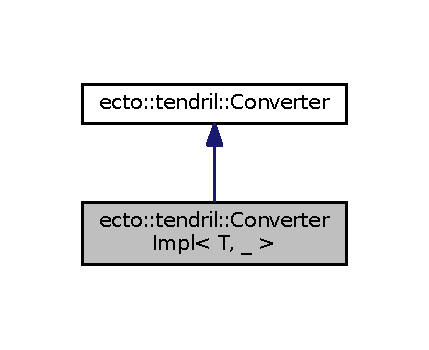
\includegraphics[width=266pt]{structecto_1_1tendril_1_1ConverterImpl__inherit__graph}
\end{center}
\end{figure}


\-Collaboration diagram for ecto\-:\-:tendril\-:\-:\-Converter\-Impl$<$ \-T, \-\_\- $>$\-:\nopagebreak
\begin{figure}[H]
\begin{center}
\leavevmode
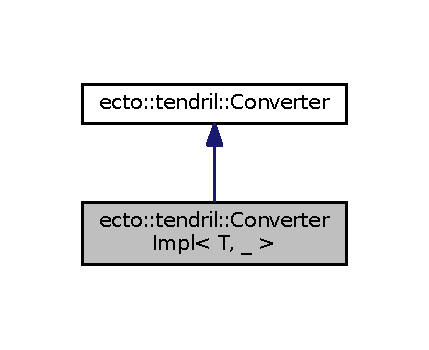
\includegraphics[width=266pt]{structecto_1_1tendril_1_1ConverterImpl__coll__graph}
\end{center}
\end{figure}
\subsection*{\-Public \-Member \-Functions}
\begin{DoxyCompactItemize}
\item 
void \hyperlink{structecto_1_1tendril_1_1ConverterImpl_aa03b80197057d2810198e3029a150988}{operator()} (\hyperlink{classecto_1_1tendril}{tendril} \&t, const boost\-::python\-::object \&obj) const 
\item 
void \hyperlink{structecto_1_1tendril_1_1ConverterImpl_a1b9b248c9a7386b8b34a436f0c8453c1}{operator()} (boost\-::python\-::object \&o, const \hyperlink{classecto_1_1tendril}{tendril} \&t) const 
\end{DoxyCompactItemize}
\subsection*{\-Static \-Public \-Attributes}
\begin{DoxyCompactItemize}
\item 
static \hyperlink{structecto_1_1tendril_1_1ConverterImpl}{\-Converter\-Impl}$<$ \-T, \-\_\- $>$ \hyperlink{structecto_1_1tendril_1_1ConverterImpl_a83cf7da46b5af2bd54127a324103c55a}{instance}
\end{DoxyCompactItemize}
\subsubsection*{template$<$typename T, typename \-\_\- = void$>$ struct ecto\-::tendril\-::\-Converter\-Impl$<$ T, \-\_\- $>$}



\subsection{\-Member \-Function \-Documentation}
\hypertarget{structecto_1_1tendril_1_1ConverterImpl_aa03b80197057d2810198e3029a150988}{\index{ecto\-::tendril\-::\-Converter\-Impl@{ecto\-::tendril\-::\-Converter\-Impl}!operator()@{operator()}}
\index{operator()@{operator()}!ecto::tendril::ConverterImpl@{ecto\-::tendril\-::\-Converter\-Impl}}
\subsubsection[{operator()}]{\setlength{\rightskip}{0pt plus 5cm}template$<$typename T , typename \-\_\-  = void$>$ void {\bf ecto\-::tendril\-::\-Converter\-Impl}$<$ \-T, \-\_\- $>$\-::operator() (
\begin{DoxyParamCaption}
\item[{{\bf tendril} \&}]{t, }
\item[{const boost\-::python\-::object \&}]{obj}
\end{DoxyParamCaption}
) const\hspace{0.3cm}{\ttfamily  \mbox{[}inline, virtual\mbox{]}}}}\label{structecto_1_1tendril_1_1ConverterImpl_aa03b80197057d2810198e3029a150988}


\-Implements \hyperlink{structecto_1_1tendril_1_1Converter_a9987df3be3c0657bea97eeeaa190e48a}{ecto\-::tendril\-::\-Converter}.

\hypertarget{structecto_1_1tendril_1_1ConverterImpl_a1b9b248c9a7386b8b34a436f0c8453c1}{\index{ecto\-::tendril\-::\-Converter\-Impl@{ecto\-::tendril\-::\-Converter\-Impl}!operator()@{operator()}}
\index{operator()@{operator()}!ecto::tendril::ConverterImpl@{ecto\-::tendril\-::\-Converter\-Impl}}
\subsubsection[{operator()}]{\setlength{\rightskip}{0pt plus 5cm}template$<$typename T , typename \-\_\-  = void$>$ void {\bf ecto\-::tendril\-::\-Converter\-Impl}$<$ \-T, \-\_\- $>$\-::operator() (
\begin{DoxyParamCaption}
\item[{boost\-::python\-::object \&}]{o, }
\item[{const {\bf tendril} \&}]{t}
\end{DoxyParamCaption}
) const\hspace{0.3cm}{\ttfamily  \mbox{[}inline, virtual\mbox{]}}}}\label{structecto_1_1tendril_1_1ConverterImpl_a1b9b248c9a7386b8b34a436f0c8453c1}


\-Implements \hyperlink{structecto_1_1tendril_1_1Converter_a73562ca297e0c5d1c6fef136701f50d3}{ecto\-::tendril\-::\-Converter}.



\subsection{\-Member \-Data \-Documentation}
\hypertarget{structecto_1_1tendril_1_1ConverterImpl_a83cf7da46b5af2bd54127a324103c55a}{\index{ecto\-::tendril\-::\-Converter\-Impl@{ecto\-::tendril\-::\-Converter\-Impl}!instance@{instance}}
\index{instance@{instance}!ecto::tendril::ConverterImpl@{ecto\-::tendril\-::\-Converter\-Impl}}
\subsubsection[{instance}]{\setlength{\rightskip}{0pt plus 5cm}template$<$typename T , typename \-\_\-  = void$>$ {\bf tendril\-::\-Converter\-Impl}$<$ {\bf tendril\-::none}, \-\_\- $>$ {\bf ecto\-::tendril\-::\-Converter\-Impl}$<$ \-\_\- $>$\-::{\bf instance}\hspace{0.3cm}{\ttfamily  \mbox{[}static\mbox{]}}}}\label{structecto_1_1tendril_1_1ConverterImpl_a83cf7da46b5af2bd54127a324103c55a}


\-The documentation for this struct was generated from the following file\-:\begin{DoxyCompactItemize}
\item 
/home/vrabaud/workspace/recognition\-\_\-kitchen\-\_\-groovy/src/ecto/include/ecto/\hyperlink{tendril_8hpp}{tendril.\-hpp}\end{DoxyCompactItemize}

\hypertarget{structecto_1_1tendril_1_1ConverterImpl_3_01none_00_01___01_4}{\section{ecto\-:\-:tendril\-:\-:Converter\-Impl$<$ none, \-\_\- $>$ Struct Template Reference}
\label{structecto_1_1tendril_1_1ConverterImpl_3_01none_00_01___01_4}\index{ecto\-::tendril\-::\-Converter\-Impl$<$ none, \-\_\- $>$@{ecto\-::tendril\-::\-Converter\-Impl$<$ none, \-\_\- $>$}}
}


Inheritance diagram for ecto\-:\-:tendril\-:\-:Converter\-Impl$<$ none, \-\_\- $>$\-:\nopagebreak
\begin{figure}[H]
\begin{center}
\leavevmode
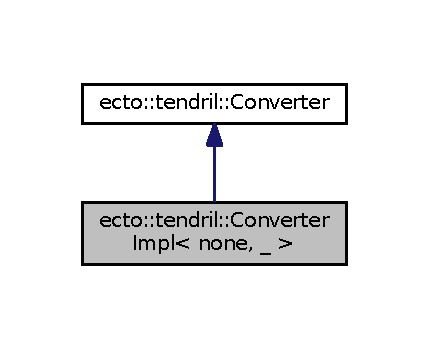
\includegraphics[width=206pt]{structecto_1_1tendril_1_1ConverterImpl_3_01none_00_01___01_4__inherit__graph}
\end{center}
\end{figure}


Collaboration diagram for ecto\-:\-:tendril\-:\-:Converter\-Impl$<$ none, \-\_\- $>$\-:\nopagebreak
\begin{figure}[H]
\begin{center}
\leavevmode
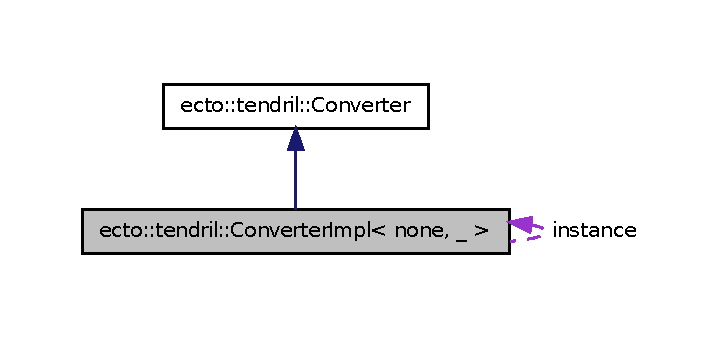
\includegraphics[width=350pt]{structecto_1_1tendril_1_1ConverterImpl_3_01none_00_01___01_4__coll__graph}
\end{center}
\end{figure}
\subsection*{Public Member Functions}
\begin{DoxyCompactItemize}
\item 
void \hyperlink{structecto_1_1tendril_1_1ConverterImpl_3_01none_00_01___01_4_ac139edd43cc2f8371eee89ed029166d4}{operator()} (\hyperlink{classecto_1_1tendril}{tendril} \&t, const boost\-::python\-::object \&obj) const 
\item 
void \hyperlink{structecto_1_1tendril_1_1ConverterImpl_3_01none_00_01___01_4_afbc6677e2eacb4352bff1b6f2aa94eee}{operator()} (boost\-::python\-::object \&o, const \hyperlink{classecto_1_1tendril}{tendril} \&t) const 
\end{DoxyCompactItemize}
\subsection*{Static Public Attributes}
\begin{DoxyCompactItemize}
\item 
static \hyperlink{structecto_1_1tendril_1_1ConverterImpl}{Converter\-Impl}$<$ \hyperlink{structecto_1_1tendril_1_1none}{none}, \-\_\- $>$ \hyperlink{structecto_1_1tendril_1_1ConverterImpl_3_01none_00_01___01_4_ace0ef7c82a522142f1821f274541c09c}{instance}
\end{DoxyCompactItemize}


\subsection{Member Function Documentation}
\hypertarget{structecto_1_1tendril_1_1ConverterImpl_3_01none_00_01___01_4_ac139edd43cc2f8371eee89ed029166d4}{\index{ecto\-::tendril\-::\-Converter\-Impl$<$ none, \-\_\- $>$@{ecto\-::tendril\-::\-Converter\-Impl$<$ none, \-\_\- $>$}!operator()@{operator()}}
\index{operator()@{operator()}!ecto::tendril::ConverterImpl< none, _ >@{ecto\-::tendril\-::\-Converter\-Impl$<$ none, \-\_\- $>$}}
\subsubsection[{operator()}]{\setlength{\rightskip}{0pt plus 5cm}template$<$typename \-\_\- $>$ void {\bf ecto\-::tendril\-::\-Converter\-Impl}$<$ {\bf none}, \-\_\- $>$\-::operator() (
\begin{DoxyParamCaption}
\item[{{\bf tendril} \&}]{t, }
\item[{const boost\-::python\-::object \&}]{obj}
\end{DoxyParamCaption}
) const\hspace{0.3cm}{\ttfamily [inline]}, {\ttfamily [virtual]}}}\label{structecto_1_1tendril_1_1ConverterImpl_3_01none_00_01___01_4_ac139edd43cc2f8371eee89ed029166d4}


Implements \hyperlink{structecto_1_1tendril_1_1Converter_a9987df3be3c0657bea97eeeaa190e48a}{ecto\-::tendril\-::\-Converter}.

\hypertarget{structecto_1_1tendril_1_1ConverterImpl_3_01none_00_01___01_4_afbc6677e2eacb4352bff1b6f2aa94eee}{\index{ecto\-::tendril\-::\-Converter\-Impl$<$ none, \-\_\- $>$@{ecto\-::tendril\-::\-Converter\-Impl$<$ none, \-\_\- $>$}!operator()@{operator()}}
\index{operator()@{operator()}!ecto::tendril::ConverterImpl< none, _ >@{ecto\-::tendril\-::\-Converter\-Impl$<$ none, \-\_\- $>$}}
\subsubsection[{operator()}]{\setlength{\rightskip}{0pt plus 5cm}template$<$typename \-\_\- $>$ void {\bf ecto\-::tendril\-::\-Converter\-Impl}$<$ {\bf none}, \-\_\- $>$\-::operator() (
\begin{DoxyParamCaption}
\item[{boost\-::python\-::object \&}]{o, }
\item[{const {\bf tendril} \&}]{t}
\end{DoxyParamCaption}
) const\hspace{0.3cm}{\ttfamily [inline]}, {\ttfamily [virtual]}}}\label{structecto_1_1tendril_1_1ConverterImpl_3_01none_00_01___01_4_afbc6677e2eacb4352bff1b6f2aa94eee}


Implements \hyperlink{structecto_1_1tendril_1_1Converter_a73562ca297e0c5d1c6fef136701f50d3}{ecto\-::tendril\-::\-Converter}.



\subsection{Member Data Documentation}
\hypertarget{structecto_1_1tendril_1_1ConverterImpl_3_01none_00_01___01_4_ace0ef7c82a522142f1821f274541c09c}{\index{ecto\-::tendril\-::\-Converter\-Impl$<$ none, \-\_\- $>$@{ecto\-::tendril\-::\-Converter\-Impl$<$ none, \-\_\- $>$}!instance@{instance}}
\index{instance@{instance}!ecto::tendril::ConverterImpl< none, _ >@{ecto\-::tendril\-::\-Converter\-Impl$<$ none, \-\_\- $>$}}
\subsubsection[{instance}]{\setlength{\rightskip}{0pt plus 5cm}template$<$typename \-\_\- $>$ {\bf Converter\-Impl}$<${\bf none}, \-\_\-$>$ {\bf ecto\-::tendril\-::\-Converter\-Impl}$<$ {\bf none}, \-\_\- $>$\-::instance\hspace{0.3cm}{\ttfamily [static]}}}\label{structecto_1_1tendril_1_1ConverterImpl_3_01none_00_01___01_4_ace0ef7c82a522142f1821f274541c09c}


The documentation for this struct was generated from the following file\-:\begin{DoxyCompactItemize}
\item 
/home/vrabaud/workspace/recognition\-\_\-kitchen/src/ecto/include/ecto/\hyperlink{tendril_8hpp}{tendril.\-hpp}\end{DoxyCompactItemize}

\hypertarget{structecto_1_1except_1_1EctoException}{\section{ecto\-:\-:except\-:\-:Ecto\-Exception Struct Reference}
\label{structecto_1_1except_1_1EctoException}\index{ecto\-::except\-::\-Ecto\-Exception@{ecto\-::except\-::\-Ecto\-Exception}}
}


{\ttfamily \#include $<$except.\-hpp$>$}



Inheritance diagram for ecto\-:\-:except\-:\-:Ecto\-Exception\-:\nopagebreak
\begin{figure}[H]
\begin{center}
\leavevmode
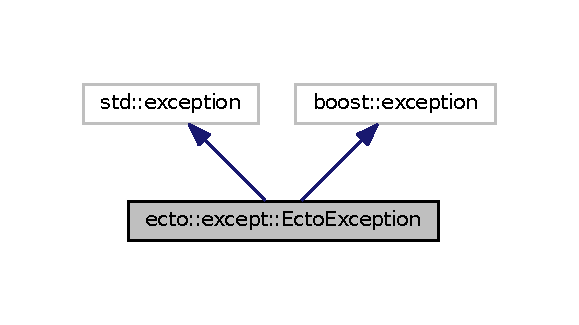
\includegraphics[width=278pt]{structecto_1_1except_1_1EctoException__inherit__graph}
\end{center}
\end{figure}


Collaboration diagram for ecto\-:\-:except\-:\-:Ecto\-Exception\-:\nopagebreak
\begin{figure}[H]
\begin{center}
\leavevmode
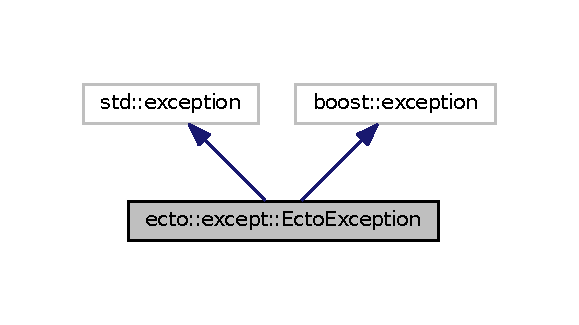
\includegraphics[width=278pt]{structecto_1_1except_1_1EctoException__coll__graph}
\end{center}
\end{figure}
\subsection*{Public Member Functions}
\begin{DoxyCompactItemize}
\item 
\hyperlink{structecto_1_1except_1_1EctoException_a5e4d1414677cf716b57620c8721b0078}{Ecto\-Exception} ()
\item 
virtual const char $\ast$ \hyperlink{structecto_1_1except_1_1EctoException_ab8f456a7153321c3424e9d6780170f4a}{what} () const   throw ()
\end{DoxyCompactItemize}


\subsection{Constructor \& Destructor Documentation}
\hypertarget{structecto_1_1except_1_1EctoException_a5e4d1414677cf716b57620c8721b0078}{\index{ecto\-::except\-::\-Ecto\-Exception@{ecto\-::except\-::\-Ecto\-Exception}!Ecto\-Exception@{Ecto\-Exception}}
\index{Ecto\-Exception@{Ecto\-Exception}!ecto::except::EctoException@{ecto\-::except\-::\-Ecto\-Exception}}
\subsubsection[{Ecto\-Exception}]{\setlength{\rightskip}{0pt plus 5cm}ecto\-::except\-::\-Ecto\-Exception\-::\-Ecto\-Exception (
\begin{DoxyParamCaption}
{}
\end{DoxyParamCaption}
)}}\label{structecto_1_1except_1_1EctoException_a5e4d1414677cf716b57620c8721b0078}


\subsection{Member Function Documentation}
\hypertarget{structecto_1_1except_1_1EctoException_ab8f456a7153321c3424e9d6780170f4a}{\index{ecto\-::except\-::\-Ecto\-Exception@{ecto\-::except\-::\-Ecto\-Exception}!what@{what}}
\index{what@{what}!ecto::except::EctoException@{ecto\-::except\-::\-Ecto\-Exception}}
\subsubsection[{what}]{\setlength{\rightskip}{0pt plus 5cm}virtual const char$\ast$ ecto\-::except\-::\-Ecto\-Exception\-::what (
\begin{DoxyParamCaption}
{}
\end{DoxyParamCaption}
) const throw  ) \hspace{0.3cm}{\ttfamily [virtual]}}}\label{structecto_1_1except_1_1EctoException_ab8f456a7153321c3424e9d6780170f4a}


The documentation for this struct was generated from the following file\-:\begin{DoxyCompactItemize}
\item 
/home/vrabaud/workspace/recognition\-\_\-kitchen/src/ecto/include/ecto/\hyperlink{except_8hpp}{except.\-hpp}\end{DoxyCompactItemize}

\hypertarget{structecto_1_1graph_1_1edge}{}\section{ecto\+:\+:graph\+:\+:edge Struct Reference}
\label{structecto_1_1graph_1_1edge}\index{ecto\+::graph\+::edge@{ecto\+::graph\+::edge}}


{\ttfamily \#include $<$edge.\+hpp$>$}



Inheritance diagram for ecto\+:\+:graph\+:\+:edge\+:\nopagebreak
\begin{figure}[H]
\begin{center}
\leavevmode
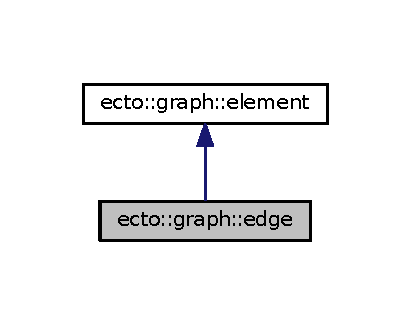
\includegraphics[width=197pt]{structecto_1_1graph_1_1edge__inherit__graph}
\end{center}
\end{figure}


Collaboration diagram for ecto\+:\+:graph\+:\+:edge\+:\nopagebreak
\begin{figure}[H]
\begin{center}
\leavevmode
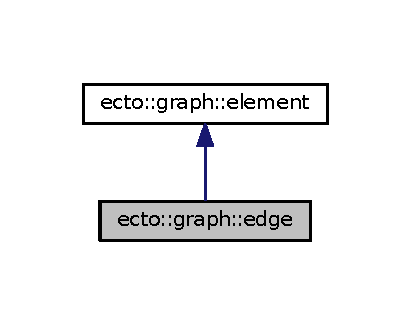
\includegraphics[width=197pt]{structecto_1_1graph_1_1edge__coll__graph}
\end{center}
\end{figure}
\subsection*{Public Member Functions}
\begin{DoxyCompactItemize}
\item 
\hyperlink{structecto_1_1graph_1_1edge_a8006b69871f55450b8acec6ac05762d4}{edge} (const std\+::string \&fp, const std\+::string \&tp)
\item 
const std\+::string \& \hyperlink{structecto_1_1graph_1_1edge_a2fb1c33fc4d337b719a1666eab943da5}{from\+\_\+port} () const 
\item 
const std\+::string \& \hyperlink{structecto_1_1graph_1_1edge_ab1c782c9d14a3f58504783747e14f7e0}{to\+\_\+port} () const 
\item 
\hyperlink{classecto_1_1tendril}{tendril} \& \hyperlink{structecto_1_1graph_1_1edge_ac2cd2d873aa55199e44f836ffada307e}{front} () const 
\item 
void \hyperlink{structecto_1_1graph_1_1edge_a0b530770694143bc00bc6c563b64a3c9}{pop\+\_\+front} ()
\item 
void \hyperlink{structecto_1_1graph_1_1edge_a257de20468c8c1b6c606448ba39c493c}{push\+\_\+back} (const \hyperlink{classecto_1_1tendril}{ecto\+::tendril} \&t)
\item 
std\+::size\+\_\+t \hyperlink{structecto_1_1graph_1_1edge_a539c89ca50c781c95ece29f7cade4d1d}{size} () const 
\item 
bool \hyperlink{structecto_1_1graph_1_1edge_ab8857a18a55e6d230e84a2a07242d67e}{empty} () const 
\item 
void \hyperlink{structecto_1_1graph_1_1edge_a2761342510ae1bedb1c91bbbda5f46ef}{clear} ()
\end{DoxyCompactItemize}
\subsection*{Private Attributes}
\begin{DoxyCompactItemize}
\item 
boost\+::shared\+\_\+ptr$<$ impl $>$ \hyperlink{structecto_1_1graph_1_1edge_a88b7d991f162cd009884c3061da8169d}{impl\+\_\+}
\end{DoxyCompactItemize}


\subsection{Constructor \& Destructor Documentation}
\index{ecto\+::graph\+::edge@{ecto\+::graph\+::edge}!edge@{edge}}
\index{edge@{edge}!ecto\+::graph\+::edge@{ecto\+::graph\+::edge}}
\subsubsection[{\texorpdfstring{edge(const std\+::string \&fp, const std\+::string \&tp)}{edge(const std::string &fp, const std::string &tp)}}]{\setlength{\rightskip}{0pt plus 5cm}ecto\+::graph\+::edge\+::edge (
\begin{DoxyParamCaption}
\item[{const std\+::string \&}]{fp, }
\item[{const std\+::string \&}]{tp}
\end{DoxyParamCaption}
)}\hypertarget{structecto_1_1graph_1_1edge_a8006b69871f55450b8acec6ac05762d4}{}\label{structecto_1_1graph_1_1edge_a8006b69871f55450b8acec6ac05762d4}


\subsection{Member Function Documentation}
\index{ecto\+::graph\+::edge@{ecto\+::graph\+::edge}!clear@{clear}}
\index{clear@{clear}!ecto\+::graph\+::edge@{ecto\+::graph\+::edge}}
\subsubsection[{\texorpdfstring{clear()}{clear()}}]{\setlength{\rightskip}{0pt plus 5cm}void ecto\+::graph\+::edge\+::clear (
\begin{DoxyParamCaption}
{}
\end{DoxyParamCaption}
)}\hypertarget{structecto_1_1graph_1_1edge_a2761342510ae1bedb1c91bbbda5f46ef}{}\label{structecto_1_1graph_1_1edge_a2761342510ae1bedb1c91bbbda5f46ef}
\index{ecto\+::graph\+::edge@{ecto\+::graph\+::edge}!empty@{empty}}
\index{empty@{empty}!ecto\+::graph\+::edge@{ecto\+::graph\+::edge}}
\subsubsection[{\texorpdfstring{empty() const }{empty() const }}]{\setlength{\rightskip}{0pt plus 5cm}bool ecto\+::graph\+::edge\+::empty (
\begin{DoxyParamCaption}
{}
\end{DoxyParamCaption}
) const}\hypertarget{structecto_1_1graph_1_1edge_ab8857a18a55e6d230e84a2a07242d67e}{}\label{structecto_1_1graph_1_1edge_ab8857a18a55e6d230e84a2a07242d67e}
\index{ecto\+::graph\+::edge@{ecto\+::graph\+::edge}!from\+\_\+port@{from\+\_\+port}}
\index{from\+\_\+port@{from\+\_\+port}!ecto\+::graph\+::edge@{ecto\+::graph\+::edge}}
\subsubsection[{\texorpdfstring{from\+\_\+port() const }{from_port() const }}]{\setlength{\rightskip}{0pt plus 5cm}const std\+::string\& ecto\+::graph\+::edge\+::from\+\_\+port (
\begin{DoxyParamCaption}
{}
\end{DoxyParamCaption}
) const}\hypertarget{structecto_1_1graph_1_1edge_a2fb1c33fc4d337b719a1666eab943da5}{}\label{structecto_1_1graph_1_1edge_a2fb1c33fc4d337b719a1666eab943da5}
\index{ecto\+::graph\+::edge@{ecto\+::graph\+::edge}!front@{front}}
\index{front@{front}!ecto\+::graph\+::edge@{ecto\+::graph\+::edge}}
\subsubsection[{\texorpdfstring{front() const }{front() const }}]{\setlength{\rightskip}{0pt plus 5cm}{\bf tendril}\& ecto\+::graph\+::edge\+::front (
\begin{DoxyParamCaption}
{}
\end{DoxyParamCaption}
) const}\hypertarget{structecto_1_1graph_1_1edge_ac2cd2d873aa55199e44f836ffada307e}{}\label{structecto_1_1graph_1_1edge_ac2cd2d873aa55199e44f836ffada307e}
\index{ecto\+::graph\+::edge@{ecto\+::graph\+::edge}!pop\+\_\+front@{pop\+\_\+front}}
\index{pop\+\_\+front@{pop\+\_\+front}!ecto\+::graph\+::edge@{ecto\+::graph\+::edge}}
\subsubsection[{\texorpdfstring{pop\+\_\+front()}{pop_front()}}]{\setlength{\rightskip}{0pt plus 5cm}void ecto\+::graph\+::edge\+::pop\+\_\+front (
\begin{DoxyParamCaption}
{}
\end{DoxyParamCaption}
)}\hypertarget{structecto_1_1graph_1_1edge_a0b530770694143bc00bc6c563b64a3c9}{}\label{structecto_1_1graph_1_1edge_a0b530770694143bc00bc6c563b64a3c9}
\index{ecto\+::graph\+::edge@{ecto\+::graph\+::edge}!push\+\_\+back@{push\+\_\+back}}
\index{push\+\_\+back@{push\+\_\+back}!ecto\+::graph\+::edge@{ecto\+::graph\+::edge}}
\subsubsection[{\texorpdfstring{push\+\_\+back(const ecto\+::tendril \&t)}{push_back(const ecto::tendril &t)}}]{\setlength{\rightskip}{0pt plus 5cm}void ecto\+::graph\+::edge\+::push\+\_\+back (
\begin{DoxyParamCaption}
\item[{const {\bf ecto\+::tendril} \&}]{t}
\end{DoxyParamCaption}
)}\hypertarget{structecto_1_1graph_1_1edge_a257de20468c8c1b6c606448ba39c493c}{}\label{structecto_1_1graph_1_1edge_a257de20468c8c1b6c606448ba39c493c}
\index{ecto\+::graph\+::edge@{ecto\+::graph\+::edge}!size@{size}}
\index{size@{size}!ecto\+::graph\+::edge@{ecto\+::graph\+::edge}}
\subsubsection[{\texorpdfstring{size() const }{size() const }}]{\setlength{\rightskip}{0pt plus 5cm}std\+::size\+\_\+t ecto\+::graph\+::edge\+::size (
\begin{DoxyParamCaption}
{}
\end{DoxyParamCaption}
) const}\hypertarget{structecto_1_1graph_1_1edge_a539c89ca50c781c95ece29f7cade4d1d}{}\label{structecto_1_1graph_1_1edge_a539c89ca50c781c95ece29f7cade4d1d}
\index{ecto\+::graph\+::edge@{ecto\+::graph\+::edge}!to\+\_\+port@{to\+\_\+port}}
\index{to\+\_\+port@{to\+\_\+port}!ecto\+::graph\+::edge@{ecto\+::graph\+::edge}}
\subsubsection[{\texorpdfstring{to\+\_\+port() const }{to_port() const }}]{\setlength{\rightskip}{0pt plus 5cm}const std\+::string\& ecto\+::graph\+::edge\+::to\+\_\+port (
\begin{DoxyParamCaption}
{}
\end{DoxyParamCaption}
) const}\hypertarget{structecto_1_1graph_1_1edge_ab1c782c9d14a3f58504783747e14f7e0}{}\label{structecto_1_1graph_1_1edge_ab1c782c9d14a3f58504783747e14f7e0}


\subsection{Member Data Documentation}
\index{ecto\+::graph\+::edge@{ecto\+::graph\+::edge}!impl\+\_\+@{impl\+\_\+}}
\index{impl\+\_\+@{impl\+\_\+}!ecto\+::graph\+::edge@{ecto\+::graph\+::edge}}
\subsubsection[{\texorpdfstring{impl\+\_\+}{impl_}}]{\setlength{\rightskip}{0pt plus 5cm}boost\+::shared\+\_\+ptr$<$impl$>$ ecto\+::graph\+::edge\+::impl\+\_\+\hspace{0.3cm}{\ttfamily [private]}}\hypertarget{structecto_1_1graph_1_1edge_a88b7d991f162cd009884c3061da8169d}{}\label{structecto_1_1graph_1_1edge_a88b7d991f162cd009884c3061da8169d}


The documentation for this struct was generated from the following file\+:\begin{DoxyCompactItemize}
\item 
/home/vrabaud/workspace/recognition\+\_\+kitchen/src/ecto/include/ecto/\hyperlink{edge_8hpp}{edge.\+hpp}\end{DoxyCompactItemize}

\hypertarget{classecto_1_1graph_1_1element}{\section{ecto\-:\-:graph\-:\-:element Class Reference}
\label{classecto_1_1graph_1_1element}\index{ecto\-::graph\-::element@{ecto\-::graph\-::element}}
}


{\ttfamily \#include $<$element.\-hpp$>$}



Inheritance diagram for ecto\-:\-:graph\-:\-:element\-:\nopagebreak
\begin{figure}[H]
\begin{center}
\leavevmode
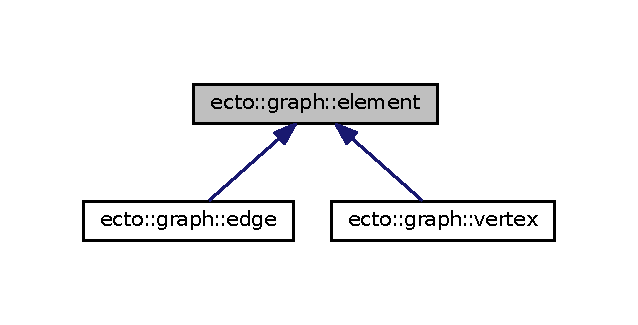
\includegraphics[width=310pt]{classecto_1_1graph_1_1element__inherit__graph}
\end{center}
\end{figure}
\subsection*{Public Member Functions}
\begin{DoxyCompactItemize}
\item 
\hyperlink{classecto_1_1graph_1_1element_abf5d2137a1fd29f25af2b8f6bd0397df}{element} ()
\item 
std\-::size\-\_\-t \hyperlink{classecto_1_1graph_1_1element_a966b0c7cd87bdc5c5787d9b110966d8f}{tick} () const 
\item 
void \hyperlink{classecto_1_1graph_1_1element_a5d5b283bacb5371285e27c0f42e54985}{inc\-\_\-tick} ()
\item 
void \hyperlink{classecto_1_1graph_1_1element_a6417601ffd8159b6e00f2ff57eda1b99}{reset\-\_\-tick} ()
\end{DoxyCompactItemize}
\subsection*{Private Attributes}
\begin{DoxyCompactItemize}
\item 
std\-::size\-\_\-t \hyperlink{classecto_1_1graph_1_1element_a6f850cead9edb37941344fdbd40ae112}{tick\-\_\-}
\end{DoxyCompactItemize}


\subsection{Constructor \& Destructor Documentation}
\hypertarget{classecto_1_1graph_1_1element_abf5d2137a1fd29f25af2b8f6bd0397df}{\index{ecto\-::graph\-::element@{ecto\-::graph\-::element}!element@{element}}
\index{element@{element}!ecto::graph::element@{ecto\-::graph\-::element}}
\subsubsection[{element}]{\setlength{\rightskip}{0pt plus 5cm}ecto\-::graph\-::element\-::element (
\begin{DoxyParamCaption}
{}
\end{DoxyParamCaption}
)\hspace{0.3cm}{\ttfamily [inline]}}}\label{classecto_1_1graph_1_1element_abf5d2137a1fd29f25af2b8f6bd0397df}


\subsection{Member Function Documentation}
\hypertarget{classecto_1_1graph_1_1element_a5d5b283bacb5371285e27c0f42e54985}{\index{ecto\-::graph\-::element@{ecto\-::graph\-::element}!inc\-\_\-tick@{inc\-\_\-tick}}
\index{inc\-\_\-tick@{inc\-\_\-tick}!ecto::graph::element@{ecto\-::graph\-::element}}
\subsubsection[{inc\-\_\-tick}]{\setlength{\rightskip}{0pt plus 5cm}void ecto\-::graph\-::element\-::inc\-\_\-tick (
\begin{DoxyParamCaption}
{}
\end{DoxyParamCaption}
)\hspace{0.3cm}{\ttfamily [inline]}}}\label{classecto_1_1graph_1_1element_a5d5b283bacb5371285e27c0f42e54985}
\hypertarget{classecto_1_1graph_1_1element_a6417601ffd8159b6e00f2ff57eda1b99}{\index{ecto\-::graph\-::element@{ecto\-::graph\-::element}!reset\-\_\-tick@{reset\-\_\-tick}}
\index{reset\-\_\-tick@{reset\-\_\-tick}!ecto::graph::element@{ecto\-::graph\-::element}}
\subsubsection[{reset\-\_\-tick}]{\setlength{\rightskip}{0pt plus 5cm}void ecto\-::graph\-::element\-::reset\-\_\-tick (
\begin{DoxyParamCaption}
{}
\end{DoxyParamCaption}
)\hspace{0.3cm}{\ttfamily [inline]}}}\label{classecto_1_1graph_1_1element_a6417601ffd8159b6e00f2ff57eda1b99}
\hypertarget{classecto_1_1graph_1_1element_a966b0c7cd87bdc5c5787d9b110966d8f}{\index{ecto\-::graph\-::element@{ecto\-::graph\-::element}!tick@{tick}}
\index{tick@{tick}!ecto::graph::element@{ecto\-::graph\-::element}}
\subsubsection[{tick}]{\setlength{\rightskip}{0pt plus 5cm}std\-::size\-\_\-t ecto\-::graph\-::element\-::tick (
\begin{DoxyParamCaption}
{}
\end{DoxyParamCaption}
) const\hspace{0.3cm}{\ttfamily [inline]}}}\label{classecto_1_1graph_1_1element_a966b0c7cd87bdc5c5787d9b110966d8f}


\subsection{Member Data Documentation}
\hypertarget{classecto_1_1graph_1_1element_a6f850cead9edb37941344fdbd40ae112}{\index{ecto\-::graph\-::element@{ecto\-::graph\-::element}!tick\-\_\-@{tick\-\_\-}}
\index{tick\-\_\-@{tick\-\_\-}!ecto::graph::element@{ecto\-::graph\-::element}}
\subsubsection[{tick\-\_\-}]{\setlength{\rightskip}{0pt plus 5cm}std\-::size\-\_\-t ecto\-::graph\-::element\-::tick\-\_\-\hspace{0.3cm}{\ttfamily [private]}}}\label{classecto_1_1graph_1_1element_a6f850cead9edb37941344fdbd40ae112}


The documentation for this class was generated from the following file\-:\begin{DoxyCompactItemize}
\item 
/home/vrabaud/workspace/recognition\-\_\-kitchen/src/ecto/include/ecto/\hyperlink{element_8hpp}{element.\-hpp}\end{DoxyCompactItemize}

\hypertarget{structecto_1_1tendril_1_1empty__t}{\section{ecto\-:\-:tendril\-:\-:empty\-\_\-t \-Struct \-Reference}
\label{structecto_1_1tendril_1_1empty__t}\index{ecto\-::tendril\-::empty\-\_\-t@{ecto\-::tendril\-::empty\-\_\-t}}
}


{\ttfamily \#include $<$tendril.\-hpp$>$}



\-The documentation for this struct was generated from the following file\-:\begin{DoxyCompactItemize}
\item 
/home/vrabaud/workspace/recognition\-\_\-kitchen\-\_\-groovy/src/ecto/include/ecto/\hyperlink{tendril_8hpp}{tendril.\-hpp}\end{DoxyCompactItemize}

\hypertarget{structecto_1_1registry_1_1tendril_1_1entry}{}\section{ecto\+:\+:registry\+:\+:tendril\+:\+:entry$<$ T $>$ Struct Template Reference}
\label{structecto_1_1registry_1_1tendril_1_1entry}\index{ecto\+::registry\+::tendril\+::entry$<$ T $>$@{ecto\+::registry\+::tendril\+::entry$<$ T $>$}}


{\ttfamily \#include $<$tendril.\+hpp$>$}

\subsection*{Public Member Functions}
\begin{DoxyCompactItemize}
\item 
\hyperlink{structecto_1_1registry_1_1tendril_1_1entry_a0e06055b642fe5a4a769276ba39fde24}{entry} (const \hyperlink{classecto_1_1tendril}{ecto\+::tendril} \&t)
\end{DoxyCompactItemize}


\subsection{Constructor \& Destructor Documentation}
\index{ecto\+::registry\+::tendril\+::entry@{ecto\+::registry\+::tendril\+::entry}!entry@{entry}}
\index{entry@{entry}!ecto\+::registry\+::tendril\+::entry@{ecto\+::registry\+::tendril\+::entry}}
\subsubsection[{\texorpdfstring{entry(const ecto\+::tendril \&t)}{entry(const ecto::tendril &t)}}]{\setlength{\rightskip}{0pt plus 5cm}template$<$typename T$>$ {\bf ecto\+::registry\+::tendril\+::entry}$<$ T $>$\+::{\bf entry} (
\begin{DoxyParamCaption}
\item[{const {\bf ecto\+::tendril} \&}]{t}
\end{DoxyParamCaption}
)\hspace{0.3cm}{\ttfamily [inline]}}\hypertarget{structecto_1_1registry_1_1tendril_1_1entry_a0e06055b642fe5a4a769276ba39fde24}{}\label{structecto_1_1registry_1_1tendril_1_1entry_a0e06055b642fe5a4a769276ba39fde24}


The documentation for this struct was generated from the following file\+:\begin{DoxyCompactItemize}
\item 
/home/vrabaud/workspace/recognition\+\_\+kitchen/src/ecto/include/ecto/\hyperlink{tendril_8hpp}{tendril.\+hpp}\end{DoxyCompactItemize}

\hypertarget{structecto_1_1registry_1_1entry__t}{\section{ecto\-:\-:registry\-:\-:entry\-\_\-t Struct Reference}
\label{structecto_1_1registry_1_1entry__t}\index{ecto\-::registry\-::entry\-\_\-t@{ecto\-::registry\-::entry\-\_\-t}}
}


{\ttfamily \#include $<$registry.\-hpp$>$}



Collaboration diagram for ecto\-:\-:registry\-:\-:entry\-\_\-t\-:\nopagebreak
\begin{figure}[H]
\begin{center}
\leavevmode
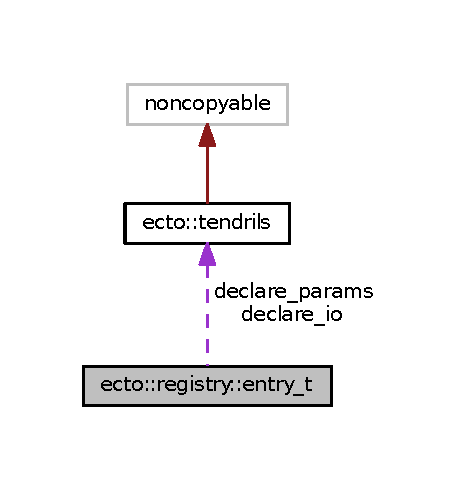
\includegraphics[width=220pt]{structecto_1_1registry_1_1entry__t__coll__graph}
\end{center}
\end{figure}
\subsection*{Public Member Functions}
\begin{DoxyCompactItemize}
\item 
boost\-::shared\-\_\-ptr$<$ \hyperlink{structecto_1_1cell}{cell} $>$ \hyperlink{structecto_1_1registry_1_1entry__t_a6690e4cc01562d27df2cca184cdd06e0}{construct\-\_\-} ()
\item 
void \hyperlink{structecto_1_1registry_1_1entry__t_af0aeb9fd69fc09b5a2b5f82841cba647}{declare\-\_\-params\-\_\-} (\hyperlink{classecto_1_1tendrils}{ecto\-::tendrils} \&t)
\item 
void \hyperlink{structecto_1_1registry_1_1entry__t_a079fd7bed79b335a8fa74c68a4ccf988}{declare\-\_\-io\-\_\-} (const \hyperlink{classecto_1_1tendrils}{ecto\-::tendrils} \&p, \hyperlink{classecto_1_1tendrils}{ecto\-::tendrils} \&i, \hyperlink{classecto_1_1tendrils}{ecto\-::tendrils} \&o)
\end{DoxyCompactItemize}
\subsection*{Public Attributes}
\begin{DoxyCompactItemize}
\item 
\hyperlink{namespaceecto_1_1registry_a3f75a16f135bcadb9bf1a7000b807b3b}{factory\-\_\-fn\-\_\-t} \hyperlink{structecto_1_1registry_1_1entry__t_ae1c1832273dbd622b1789a82f0832aa8}{construct}
\item 
\hyperlink{namespaceecto_1_1registry_a04d849b45313a8ce9a602095e1edade9}{declare\-\_\-params\-\_\-t} \hyperlink{structecto_1_1registry_1_1entry__t_a0e87799ee057b4509d45eab85def3b80}{declare\-\_\-params}
\item 
\hyperlink{namespaceecto_1_1registry_af52d8f0fff3baaf352e2523ab8ed7977}{declare\-\_\-io\-\_\-t} \hyperlink{structecto_1_1registry_1_1entry__t_ac052cec6adea69584fbb17f24e147ec2}{declare\-\_\-io}
\end{DoxyCompactItemize}


\subsection{Member Function Documentation}
\hypertarget{structecto_1_1registry_1_1entry__t_a6690e4cc01562d27df2cca184cdd06e0}{\index{ecto\-::registry\-::entry\-\_\-t@{ecto\-::registry\-::entry\-\_\-t}!construct\-\_\-@{construct\-\_\-}}
\index{construct\-\_\-@{construct\-\_\-}!ecto::registry::entry_t@{ecto\-::registry\-::entry\-\_\-t}}
\subsubsection[{construct\-\_\-}]{\setlength{\rightskip}{0pt plus 5cm}boost\-::shared\-\_\-ptr$<${\bf cell}$>$ ecto\-::registry\-::entry\-\_\-t\-::construct\-\_\- (
\begin{DoxyParamCaption}
{}
\end{DoxyParamCaption}
)\hspace{0.3cm}{\ttfamily [inline]}}}\label{structecto_1_1registry_1_1entry__t_a6690e4cc01562d27df2cca184cdd06e0}
\hypertarget{structecto_1_1registry_1_1entry__t_a079fd7bed79b335a8fa74c68a4ccf988}{\index{ecto\-::registry\-::entry\-\_\-t@{ecto\-::registry\-::entry\-\_\-t}!declare\-\_\-io\-\_\-@{declare\-\_\-io\-\_\-}}
\index{declare\-\_\-io\-\_\-@{declare\-\_\-io\-\_\-}!ecto::registry::entry_t@{ecto\-::registry\-::entry\-\_\-t}}
\subsubsection[{declare\-\_\-io\-\_\-}]{\setlength{\rightskip}{0pt plus 5cm}void ecto\-::registry\-::entry\-\_\-t\-::declare\-\_\-io\-\_\- (
\begin{DoxyParamCaption}
\item[{const {\bf ecto\-::tendrils} \&}]{p, }
\item[{{\bf ecto\-::tendrils} \&}]{i, }
\item[{{\bf ecto\-::tendrils} \&}]{o}
\end{DoxyParamCaption}
)\hspace{0.3cm}{\ttfamily [inline]}}}\label{structecto_1_1registry_1_1entry__t_a079fd7bed79b335a8fa74c68a4ccf988}
\hypertarget{structecto_1_1registry_1_1entry__t_af0aeb9fd69fc09b5a2b5f82841cba647}{\index{ecto\-::registry\-::entry\-\_\-t@{ecto\-::registry\-::entry\-\_\-t}!declare\-\_\-params\-\_\-@{declare\-\_\-params\-\_\-}}
\index{declare\-\_\-params\-\_\-@{declare\-\_\-params\-\_\-}!ecto::registry::entry_t@{ecto\-::registry\-::entry\-\_\-t}}
\subsubsection[{declare\-\_\-params\-\_\-}]{\setlength{\rightskip}{0pt plus 5cm}void ecto\-::registry\-::entry\-\_\-t\-::declare\-\_\-params\-\_\- (
\begin{DoxyParamCaption}
\item[{{\bf ecto\-::tendrils} \&}]{t}
\end{DoxyParamCaption}
)\hspace{0.3cm}{\ttfamily [inline]}}}\label{structecto_1_1registry_1_1entry__t_af0aeb9fd69fc09b5a2b5f82841cba647}


\subsection{Member Data Documentation}
\hypertarget{structecto_1_1registry_1_1entry__t_ae1c1832273dbd622b1789a82f0832aa8}{\index{ecto\-::registry\-::entry\-\_\-t@{ecto\-::registry\-::entry\-\_\-t}!construct@{construct}}
\index{construct@{construct}!ecto::registry::entry_t@{ecto\-::registry\-::entry\-\_\-t}}
\subsubsection[{construct}]{\setlength{\rightskip}{0pt plus 5cm}{\bf factory\-\_\-fn\-\_\-t} ecto\-::registry\-::entry\-\_\-t\-::construct}}\label{structecto_1_1registry_1_1entry__t_ae1c1832273dbd622b1789a82f0832aa8}
\hypertarget{structecto_1_1registry_1_1entry__t_ac052cec6adea69584fbb17f24e147ec2}{\index{ecto\-::registry\-::entry\-\_\-t@{ecto\-::registry\-::entry\-\_\-t}!declare\-\_\-io@{declare\-\_\-io}}
\index{declare\-\_\-io@{declare\-\_\-io}!ecto::registry::entry_t@{ecto\-::registry\-::entry\-\_\-t}}
\subsubsection[{declare\-\_\-io}]{\setlength{\rightskip}{0pt plus 5cm}{\bf declare\-\_\-io\-\_\-t} ecto\-::registry\-::entry\-\_\-t\-::declare\-\_\-io}}\label{structecto_1_1registry_1_1entry__t_ac052cec6adea69584fbb17f24e147ec2}
\hypertarget{structecto_1_1registry_1_1entry__t_a0e87799ee057b4509d45eab85def3b80}{\index{ecto\-::registry\-::entry\-\_\-t@{ecto\-::registry\-::entry\-\_\-t}!declare\-\_\-params@{declare\-\_\-params}}
\index{declare\-\_\-params@{declare\-\_\-params}!ecto::registry::entry_t@{ecto\-::registry\-::entry\-\_\-t}}
\subsubsection[{declare\-\_\-params}]{\setlength{\rightskip}{0pt plus 5cm}{\bf declare\-\_\-params\-\_\-t} ecto\-::registry\-::entry\-\_\-t\-::declare\-\_\-params}}\label{structecto_1_1registry_1_1entry__t_a0e87799ee057b4509d45eab85def3b80}


The documentation for this struct was generated from the following file\-:\begin{DoxyCompactItemize}
\item 
/home/vrabaud/workspace/recognition\-\_\-kitchen/src/ecto/include/ecto/\hyperlink{registry_8hpp}{registry.\-hpp}\end{DoxyCompactItemize}

\hypertarget{classecto_1_1except_1_1error__info__container__impl}{}\section{ecto\+:\+:except\+:\+:error\+\_\+info\+\_\+container\+\_\+impl Class Reference}
\label{classecto_1_1except_1_1error__info__container__impl}\index{ecto\+::except\+::error\+\_\+info\+\_\+container\+\_\+impl@{ecto\+::except\+::error\+\_\+info\+\_\+container\+\_\+impl}}


{\ttfamily \#include $<$except.\+hpp$>$}



Inheritance diagram for ecto\+:\+:except\+:\+:error\+\_\+info\+\_\+container\+\_\+impl\+:\nopagebreak
\begin{figure}[H]
\begin{center}
\leavevmode
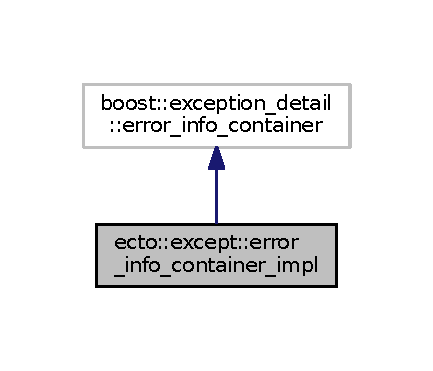
\includegraphics[width=208pt]{classecto_1_1except_1_1error__info__container__impl__inherit__graph}
\end{center}
\end{figure}


Collaboration diagram for ecto\+:\+:except\+:\+:error\+\_\+info\+\_\+container\+\_\+impl\+:\nopagebreak
\begin{figure}[H]
\begin{center}
\leavevmode
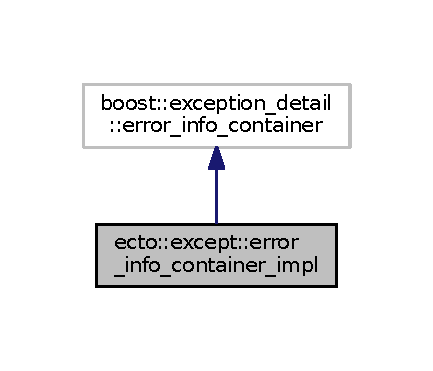
\includegraphics[width=208pt]{classecto_1_1except_1_1error__info__container__impl__coll__graph}
\end{center}
\end{figure}
\subsection*{Public Member Functions}
\begin{DoxyCompactItemize}
\item 
\hyperlink{classecto_1_1except_1_1error__info__container__impl_a258f844c2a2ee441c4e397971466f2c5}{error\+\_\+info\+\_\+container\+\_\+impl} ()
\item 
\hyperlink{classecto_1_1except_1_1error__info__container__impl_ab9391a11b1c7955810c184c07aec4858}{$\sim$error\+\_\+info\+\_\+container\+\_\+impl} ()  throw ()
\item 
void \hyperlink{classecto_1_1except_1_1error__info__container__impl_ac3931483b05bd3240a8ffe11c4977b99}{set} (\hyperlink{classecto_1_1except_1_1error__info__container__impl_a9fbca0758380cb123f790aee77d1d4d8}{error\+\_\+info\+\_\+base\+\_\+ptr} const \&x, \hyperlink{classecto_1_1except_1_1error__info__container__impl_abe4f51bf533842a5e0b81f3e43ae6267}{type\+\_\+info\+\_\+} const \&typeid\+\_\+)
\item 
\hyperlink{classecto_1_1except_1_1error__info__container__impl_a9fbca0758380cb123f790aee77d1d4d8}{error\+\_\+info\+\_\+base\+\_\+ptr} \hyperlink{classecto_1_1except_1_1error__info__container__impl_acab3219ea75b29048e2e4d8ad23028eb}{get} (\hyperlink{classecto_1_1except_1_1error__info__container__impl_abe4f51bf533842a5e0b81f3e43ae6267}{type\+\_\+info\+\_\+} const \&ti) const 
\item 
char const $\ast$ \hyperlink{classecto_1_1except_1_1error__info__container__impl_a9cd76f7d8bd75cdc5cf29061304a622a}{diagnostic\+\_\+information} () const 
\end{DoxyCompactItemize}
\subsection*{Private Types}
\begin{DoxyCompactItemize}
\item 
typedef \+::boost\+::exception\+\_\+detail\+::type\+\_\+info\+\_\+ \hyperlink{classecto_1_1except_1_1error__info__container__impl_abe4f51bf533842a5e0b81f3e43ae6267}{type\+\_\+info\+\_\+}
\item 
typedef \+::boost\+::exception\+\_\+detail\+::error\+\_\+info\+\_\+base \hyperlink{classecto_1_1except_1_1error__info__container__impl_a90c2628bf7c5628003cd24fd369a77da}{error\+\_\+info\+\_\+base}
\item 
typedef boost\+::shared\+\_\+ptr$<$ \hyperlink{classecto_1_1except_1_1error__info__container__impl_a90c2628bf7c5628003cd24fd369a77da}{error\+\_\+info\+\_\+base} $>$ \hyperlink{classecto_1_1except_1_1error__info__container__impl_a9fbca0758380cb123f790aee77d1d4d8}{error\+\_\+info\+\_\+base\+\_\+ptr}
\item 
typedef const char $\ast$ \hyperlink{classecto_1_1except_1_1error__info__container__impl_a16f5ebd1abcacd60ddbd919ea166958e}{diagnostic\+\_\+information\+\_\+arg\+\_\+t}
\item 
typedef std\+::map$<$ std\+::string, \hyperlink{classecto_1_1except_1_1error__info__container__impl_a9fbca0758380cb123f790aee77d1d4d8}{error\+\_\+info\+\_\+base\+\_\+ptr} $>$ \hyperlink{classecto_1_1except_1_1error__info__container__impl_a20b3846bc393224fe282eb64a40ee83d}{error\+\_\+info\+\_\+map}
\end{DoxyCompactItemize}
\subsection*{Private Member Functions}
\begin{DoxyCompactItemize}
\item 
void \hyperlink{classecto_1_1except_1_1error__info__container__impl_ae931c5c31454852cdf3d1a84d1d588eb}{add\+\_\+ref} () const 
\item 
bool \hyperlink{classecto_1_1except_1_1error__info__container__impl_a59b8d31c21da10236de67f0a5bfdf4dd}{release} () const 
\end{DoxyCompactItemize}
\subsection*{Private Attributes}
\begin{DoxyCompactItemize}
\item 
\hyperlink{classecto_1_1except_1_1error__info__container__impl_a20b3846bc393224fe282eb64a40ee83d}{error\+\_\+info\+\_\+map} \hyperlink{classecto_1_1except_1_1error__info__container__impl_a8ec60b174805696bd691a894b7f4109f}{info\+\_\+}
\item 
std\+::string \hyperlink{classecto_1_1except_1_1error__info__container__impl_aeb86496a5127e19e9f787e77531b1b83}{diagnostic\+\_\+info\+\_\+str\+\_\+}
\item 
int \hyperlink{classecto_1_1except_1_1error__info__container__impl_ade4abdc4aa11c62dd39847bc4f6c619c}{count\+\_\+}
\end{DoxyCompactItemize}
\subsection*{Friends}
\begin{DoxyCompactItemize}
\item 
class \hyperlink{classecto_1_1except_1_1error__info__container__impl_a17667d5fc9c440eb33937b735d4fdfe6}{boost\+::exception}
\end{DoxyCompactItemize}


\subsection{Member Typedef Documentation}
\hypertarget{classecto_1_1except_1_1error__info__container__impl_a16f5ebd1abcacd60ddbd919ea166958e}{}\index{ecto\+::except\+::error\+\_\+info\+\_\+container\+\_\+impl@{ecto\+::except\+::error\+\_\+info\+\_\+container\+\_\+impl}!diagnostic\+\_\+information\+\_\+arg\+\_\+t@{diagnostic\+\_\+information\+\_\+arg\+\_\+t}}
\index{diagnostic\+\_\+information\+\_\+arg\+\_\+t@{diagnostic\+\_\+information\+\_\+arg\+\_\+t}!ecto\+::except\+::error\+\_\+info\+\_\+container\+\_\+impl@{ecto\+::except\+::error\+\_\+info\+\_\+container\+\_\+impl}}
\subsubsection[{diagnostic\+\_\+information\+\_\+arg\+\_\+t}]{\setlength{\rightskip}{0pt plus 5cm}typedef const char$\ast$ {\bf ecto\+::except\+::error\+\_\+info\+\_\+container\+\_\+impl\+::diagnostic\+\_\+information\+\_\+arg\+\_\+t}\hspace{0.3cm}{\ttfamily [private]}}\label{classecto_1_1except_1_1error__info__container__impl_a16f5ebd1abcacd60ddbd919ea166958e}
\hypertarget{classecto_1_1except_1_1error__info__container__impl_a90c2628bf7c5628003cd24fd369a77da}{}\index{ecto\+::except\+::error\+\_\+info\+\_\+container\+\_\+impl@{ecto\+::except\+::error\+\_\+info\+\_\+container\+\_\+impl}!error\+\_\+info\+\_\+base@{error\+\_\+info\+\_\+base}}
\index{error\+\_\+info\+\_\+base@{error\+\_\+info\+\_\+base}!ecto\+::except\+::error\+\_\+info\+\_\+container\+\_\+impl@{ecto\+::except\+::error\+\_\+info\+\_\+container\+\_\+impl}}
\subsubsection[{error\+\_\+info\+\_\+base}]{\setlength{\rightskip}{0pt plus 5cm}typedef \+::boost\+::exception\+\_\+detail\+::error\+\_\+info\+\_\+base {\bf ecto\+::except\+::error\+\_\+info\+\_\+container\+\_\+impl\+::error\+\_\+info\+\_\+base}\hspace{0.3cm}{\ttfamily [private]}}\label{classecto_1_1except_1_1error__info__container__impl_a90c2628bf7c5628003cd24fd369a77da}
\hypertarget{classecto_1_1except_1_1error__info__container__impl_a9fbca0758380cb123f790aee77d1d4d8}{}\index{ecto\+::except\+::error\+\_\+info\+\_\+container\+\_\+impl@{ecto\+::except\+::error\+\_\+info\+\_\+container\+\_\+impl}!error\+\_\+info\+\_\+base\+\_\+ptr@{error\+\_\+info\+\_\+base\+\_\+ptr}}
\index{error\+\_\+info\+\_\+base\+\_\+ptr@{error\+\_\+info\+\_\+base\+\_\+ptr}!ecto\+::except\+::error\+\_\+info\+\_\+container\+\_\+impl@{ecto\+::except\+::error\+\_\+info\+\_\+container\+\_\+impl}}
\subsubsection[{error\+\_\+info\+\_\+base\+\_\+ptr}]{\setlength{\rightskip}{0pt plus 5cm}typedef boost\+::shared\+\_\+ptr$<${\bf error\+\_\+info\+\_\+base}$>$ {\bf ecto\+::except\+::error\+\_\+info\+\_\+container\+\_\+impl\+::error\+\_\+info\+\_\+base\+\_\+ptr}\hspace{0.3cm}{\ttfamily [private]}}\label{classecto_1_1except_1_1error__info__container__impl_a9fbca0758380cb123f790aee77d1d4d8}
\hypertarget{classecto_1_1except_1_1error__info__container__impl_a20b3846bc393224fe282eb64a40ee83d}{}\index{ecto\+::except\+::error\+\_\+info\+\_\+container\+\_\+impl@{ecto\+::except\+::error\+\_\+info\+\_\+container\+\_\+impl}!error\+\_\+info\+\_\+map@{error\+\_\+info\+\_\+map}}
\index{error\+\_\+info\+\_\+map@{error\+\_\+info\+\_\+map}!ecto\+::except\+::error\+\_\+info\+\_\+container\+\_\+impl@{ecto\+::except\+::error\+\_\+info\+\_\+container\+\_\+impl}}
\subsubsection[{error\+\_\+info\+\_\+map}]{\setlength{\rightskip}{0pt plus 5cm}typedef std\+::map$<$std\+::string, {\bf error\+\_\+info\+\_\+base\+\_\+ptr}$>$ {\bf ecto\+::except\+::error\+\_\+info\+\_\+container\+\_\+impl\+::error\+\_\+info\+\_\+map}\hspace{0.3cm}{\ttfamily [private]}}\label{classecto_1_1except_1_1error__info__container__impl_a20b3846bc393224fe282eb64a40ee83d}
\hypertarget{classecto_1_1except_1_1error__info__container__impl_abe4f51bf533842a5e0b81f3e43ae6267}{}\index{ecto\+::except\+::error\+\_\+info\+\_\+container\+\_\+impl@{ecto\+::except\+::error\+\_\+info\+\_\+container\+\_\+impl}!type\+\_\+info\+\_\+@{type\+\_\+info\+\_\+}}
\index{type\+\_\+info\+\_\+@{type\+\_\+info\+\_\+}!ecto\+::except\+::error\+\_\+info\+\_\+container\+\_\+impl@{ecto\+::except\+::error\+\_\+info\+\_\+container\+\_\+impl}}
\subsubsection[{type\+\_\+info\+\_\+}]{\setlength{\rightskip}{0pt plus 5cm}typedef \+::boost\+::exception\+\_\+detail\+::type\+\_\+info\+\_\+ {\bf ecto\+::except\+::error\+\_\+info\+\_\+container\+\_\+impl\+::type\+\_\+info\+\_\+}\hspace{0.3cm}{\ttfamily [private]}}\label{classecto_1_1except_1_1error__info__container__impl_abe4f51bf533842a5e0b81f3e43ae6267}


\subsection{Constructor \& Destructor Documentation}
\hypertarget{classecto_1_1except_1_1error__info__container__impl_a258f844c2a2ee441c4e397971466f2c5}{}\index{ecto\+::except\+::error\+\_\+info\+\_\+container\+\_\+impl@{ecto\+::except\+::error\+\_\+info\+\_\+container\+\_\+impl}!error\+\_\+info\+\_\+container\+\_\+impl@{error\+\_\+info\+\_\+container\+\_\+impl}}
\index{error\+\_\+info\+\_\+container\+\_\+impl@{error\+\_\+info\+\_\+container\+\_\+impl}!ecto\+::except\+::error\+\_\+info\+\_\+container\+\_\+impl@{ecto\+::except\+::error\+\_\+info\+\_\+container\+\_\+impl}}
\subsubsection[{error\+\_\+info\+\_\+container\+\_\+impl}]{\setlength{\rightskip}{0pt plus 5cm}ecto\+::except\+::error\+\_\+info\+\_\+container\+\_\+impl\+::error\+\_\+info\+\_\+container\+\_\+impl (
\begin{DoxyParamCaption}
{}
\end{DoxyParamCaption}
)}\label{classecto_1_1except_1_1error__info__container__impl_a258f844c2a2ee441c4e397971466f2c5}
\hypertarget{classecto_1_1except_1_1error__info__container__impl_ab9391a11b1c7955810c184c07aec4858}{}\index{ecto\+::except\+::error\+\_\+info\+\_\+container\+\_\+impl@{ecto\+::except\+::error\+\_\+info\+\_\+container\+\_\+impl}!````~error\+\_\+info\+\_\+container\+\_\+impl@{$\sim$error\+\_\+info\+\_\+container\+\_\+impl}}
\index{````~error\+\_\+info\+\_\+container\+\_\+impl@{$\sim$error\+\_\+info\+\_\+container\+\_\+impl}!ecto\+::except\+::error\+\_\+info\+\_\+container\+\_\+impl@{ecto\+::except\+::error\+\_\+info\+\_\+container\+\_\+impl}}
\subsubsection[{$\sim$error\+\_\+info\+\_\+container\+\_\+impl}]{\setlength{\rightskip}{0pt plus 5cm}ecto\+::except\+::error\+\_\+info\+\_\+container\+\_\+impl\+::$\sim$error\+\_\+info\+\_\+container\+\_\+impl (
\begin{DoxyParamCaption}
{}
\end{DoxyParamCaption}
) throw  ) }\label{classecto_1_1except_1_1error__info__container__impl_ab9391a11b1c7955810c184c07aec4858}


\subsection{Member Function Documentation}
\hypertarget{classecto_1_1except_1_1error__info__container__impl_ae931c5c31454852cdf3d1a84d1d588eb}{}\index{ecto\+::except\+::error\+\_\+info\+\_\+container\+\_\+impl@{ecto\+::except\+::error\+\_\+info\+\_\+container\+\_\+impl}!add\+\_\+ref@{add\+\_\+ref}}
\index{add\+\_\+ref@{add\+\_\+ref}!ecto\+::except\+::error\+\_\+info\+\_\+container\+\_\+impl@{ecto\+::except\+::error\+\_\+info\+\_\+container\+\_\+impl}}
\subsubsection[{add\+\_\+ref}]{\setlength{\rightskip}{0pt plus 5cm}void ecto\+::except\+::error\+\_\+info\+\_\+container\+\_\+impl\+::add\+\_\+ref (
\begin{DoxyParamCaption}
{}
\end{DoxyParamCaption}
) const\hspace{0.3cm}{\ttfamily [private]}}\label{classecto_1_1except_1_1error__info__container__impl_ae931c5c31454852cdf3d1a84d1d588eb}
\hypertarget{classecto_1_1except_1_1error__info__container__impl_a9cd76f7d8bd75cdc5cf29061304a622a}{}\index{ecto\+::except\+::error\+\_\+info\+\_\+container\+\_\+impl@{ecto\+::except\+::error\+\_\+info\+\_\+container\+\_\+impl}!diagnostic\+\_\+information@{diagnostic\+\_\+information}}
\index{diagnostic\+\_\+information@{diagnostic\+\_\+information}!ecto\+::except\+::error\+\_\+info\+\_\+container\+\_\+impl@{ecto\+::except\+::error\+\_\+info\+\_\+container\+\_\+impl}}
\subsubsection[{diagnostic\+\_\+information}]{\setlength{\rightskip}{0pt plus 5cm}char const$\ast$ ecto\+::except\+::error\+\_\+info\+\_\+container\+\_\+impl\+::diagnostic\+\_\+information (
\begin{DoxyParamCaption}
{}
\end{DoxyParamCaption}
) const}\label{classecto_1_1except_1_1error__info__container__impl_a9cd76f7d8bd75cdc5cf29061304a622a}
\hypertarget{classecto_1_1except_1_1error__info__container__impl_acab3219ea75b29048e2e4d8ad23028eb}{}\index{ecto\+::except\+::error\+\_\+info\+\_\+container\+\_\+impl@{ecto\+::except\+::error\+\_\+info\+\_\+container\+\_\+impl}!get@{get}}
\index{get@{get}!ecto\+::except\+::error\+\_\+info\+\_\+container\+\_\+impl@{ecto\+::except\+::error\+\_\+info\+\_\+container\+\_\+impl}}
\subsubsection[{get}]{\setlength{\rightskip}{0pt plus 5cm}{\bf error\+\_\+info\+\_\+base\+\_\+ptr} ecto\+::except\+::error\+\_\+info\+\_\+container\+\_\+impl\+::get (
\begin{DoxyParamCaption}
\item[{{\bf type\+\_\+info\+\_\+} const \&}]{ti}
\end{DoxyParamCaption}
) const}\label{classecto_1_1except_1_1error__info__container__impl_acab3219ea75b29048e2e4d8ad23028eb}
\hypertarget{classecto_1_1except_1_1error__info__container__impl_a59b8d31c21da10236de67f0a5bfdf4dd}{}\index{ecto\+::except\+::error\+\_\+info\+\_\+container\+\_\+impl@{ecto\+::except\+::error\+\_\+info\+\_\+container\+\_\+impl}!release@{release}}
\index{release@{release}!ecto\+::except\+::error\+\_\+info\+\_\+container\+\_\+impl@{ecto\+::except\+::error\+\_\+info\+\_\+container\+\_\+impl}}
\subsubsection[{release}]{\setlength{\rightskip}{0pt plus 5cm}bool ecto\+::except\+::error\+\_\+info\+\_\+container\+\_\+impl\+::release (
\begin{DoxyParamCaption}
{}
\end{DoxyParamCaption}
) const\hspace{0.3cm}{\ttfamily [private]}}\label{classecto_1_1except_1_1error__info__container__impl_a59b8d31c21da10236de67f0a5bfdf4dd}
\hypertarget{classecto_1_1except_1_1error__info__container__impl_ac3931483b05bd3240a8ffe11c4977b99}{}\index{ecto\+::except\+::error\+\_\+info\+\_\+container\+\_\+impl@{ecto\+::except\+::error\+\_\+info\+\_\+container\+\_\+impl}!set@{set}}
\index{set@{set}!ecto\+::except\+::error\+\_\+info\+\_\+container\+\_\+impl@{ecto\+::except\+::error\+\_\+info\+\_\+container\+\_\+impl}}
\subsubsection[{set}]{\setlength{\rightskip}{0pt plus 5cm}void ecto\+::except\+::error\+\_\+info\+\_\+container\+\_\+impl\+::set (
\begin{DoxyParamCaption}
\item[{{\bf error\+\_\+info\+\_\+base\+\_\+ptr} const \&}]{x, }
\item[{{\bf type\+\_\+info\+\_\+} const \&}]{typeid\+\_\+}
\end{DoxyParamCaption}
)}\label{classecto_1_1except_1_1error__info__container__impl_ac3931483b05bd3240a8ffe11c4977b99}


\subsection{Friends And Related Function Documentation}
\hypertarget{classecto_1_1except_1_1error__info__container__impl_a17667d5fc9c440eb33937b735d4fdfe6}{}\index{ecto\+::except\+::error\+\_\+info\+\_\+container\+\_\+impl@{ecto\+::except\+::error\+\_\+info\+\_\+container\+\_\+impl}!boost\+::exception@{boost\+::exception}}
\index{boost\+::exception@{boost\+::exception}!ecto\+::except\+::error\+\_\+info\+\_\+container\+\_\+impl@{ecto\+::except\+::error\+\_\+info\+\_\+container\+\_\+impl}}
\subsubsection[{boost\+::exception}]{\setlength{\rightskip}{0pt plus 5cm}friend class boost\+::exception\hspace{0.3cm}{\ttfamily [friend]}}\label{classecto_1_1except_1_1error__info__container__impl_a17667d5fc9c440eb33937b735d4fdfe6}


\subsection{Member Data Documentation}
\hypertarget{classecto_1_1except_1_1error__info__container__impl_ade4abdc4aa11c62dd39847bc4f6c619c}{}\index{ecto\+::except\+::error\+\_\+info\+\_\+container\+\_\+impl@{ecto\+::except\+::error\+\_\+info\+\_\+container\+\_\+impl}!count\+\_\+@{count\+\_\+}}
\index{count\+\_\+@{count\+\_\+}!ecto\+::except\+::error\+\_\+info\+\_\+container\+\_\+impl@{ecto\+::except\+::error\+\_\+info\+\_\+container\+\_\+impl}}
\subsubsection[{count\+\_\+}]{\setlength{\rightskip}{0pt plus 5cm}int ecto\+::except\+::error\+\_\+info\+\_\+container\+\_\+impl\+::count\+\_\+\hspace{0.3cm}{\ttfamily [mutable]}, {\ttfamily [private]}}\label{classecto_1_1except_1_1error__info__container__impl_ade4abdc4aa11c62dd39847bc4f6c619c}
\hypertarget{classecto_1_1except_1_1error__info__container__impl_aeb86496a5127e19e9f787e77531b1b83}{}\index{ecto\+::except\+::error\+\_\+info\+\_\+container\+\_\+impl@{ecto\+::except\+::error\+\_\+info\+\_\+container\+\_\+impl}!diagnostic\+\_\+info\+\_\+str\+\_\+@{diagnostic\+\_\+info\+\_\+str\+\_\+}}
\index{diagnostic\+\_\+info\+\_\+str\+\_\+@{diagnostic\+\_\+info\+\_\+str\+\_\+}!ecto\+::except\+::error\+\_\+info\+\_\+container\+\_\+impl@{ecto\+::except\+::error\+\_\+info\+\_\+container\+\_\+impl}}
\subsubsection[{diagnostic\+\_\+info\+\_\+str\+\_\+}]{\setlength{\rightskip}{0pt plus 5cm}std\+::string ecto\+::except\+::error\+\_\+info\+\_\+container\+\_\+impl\+::diagnostic\+\_\+info\+\_\+str\+\_\+\hspace{0.3cm}{\ttfamily [mutable]}, {\ttfamily [private]}}\label{classecto_1_1except_1_1error__info__container__impl_aeb86496a5127e19e9f787e77531b1b83}
\hypertarget{classecto_1_1except_1_1error__info__container__impl_a8ec60b174805696bd691a894b7f4109f}{}\index{ecto\+::except\+::error\+\_\+info\+\_\+container\+\_\+impl@{ecto\+::except\+::error\+\_\+info\+\_\+container\+\_\+impl}!info\+\_\+@{info\+\_\+}}
\index{info\+\_\+@{info\+\_\+}!ecto\+::except\+::error\+\_\+info\+\_\+container\+\_\+impl@{ecto\+::except\+::error\+\_\+info\+\_\+container\+\_\+impl}}
\subsubsection[{info\+\_\+}]{\setlength{\rightskip}{0pt plus 5cm}{\bf error\+\_\+info\+\_\+map} ecto\+::except\+::error\+\_\+info\+\_\+container\+\_\+impl\+::info\+\_\+\hspace{0.3cm}{\ttfamily [private]}}\label{classecto_1_1except_1_1error__info__container__impl_a8ec60b174805696bd691a894b7f4109f}


The documentation for this class was generated from the following file\+:\begin{DoxyCompactItemize}
\item 
/home/vrabaud/workspace/recognition\+\_\+kitchen/src/ecto/include/ecto/\hyperlink{except_8hpp}{except.\+hpp}\end{DoxyCompactItemize}

\hypertarget{classboost_1_1python_1_1detail_1_1final__std__map__derived__policies}{}\section{boost\+:\+:python\+:\+:detail\+:\+:final\+\_\+std\+\_\+map\+\_\+derived\+\_\+policies$<$ Container, No\+Proxy $>$ Class Template Reference}
\label{classboost_1_1python_1_1detail_1_1final__std__map__derived__policies}\index{boost\+::python\+::detail\+::final\+\_\+std\+\_\+map\+\_\+derived\+\_\+policies$<$ Container, No\+Proxy $>$@{boost\+::python\+::detail\+::final\+\_\+std\+\_\+map\+\_\+derived\+\_\+policies$<$ Container, No\+Proxy $>$}}


{\ttfamily \#include $<$std\+\_\+map\+\_\+indexing\+\_\+suite.\+hpp$>$}



Inheritance diagram for boost\+:\+:python\+:\+:detail\+:\+:final\+\_\+std\+\_\+map\+\_\+derived\+\_\+policies$<$ Container, No\+Proxy $>$\+:\nopagebreak
\begin{figure}[H]
\begin{center}
\leavevmode
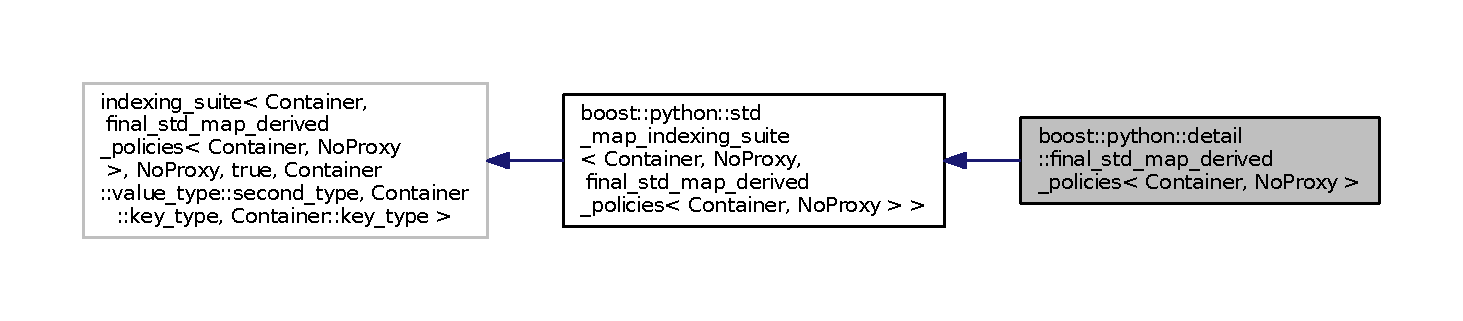
\includegraphics[width=350pt]{classboost_1_1python_1_1detail_1_1final__std__map__derived__policies__inherit__graph}
\end{center}
\end{figure}


Collaboration diagram for boost\+:\+:python\+:\+:detail\+:\+:final\+\_\+std\+\_\+map\+\_\+derived\+\_\+policies$<$ Container, No\+Proxy $>$\+:\nopagebreak
\begin{figure}[H]
\begin{center}
\leavevmode
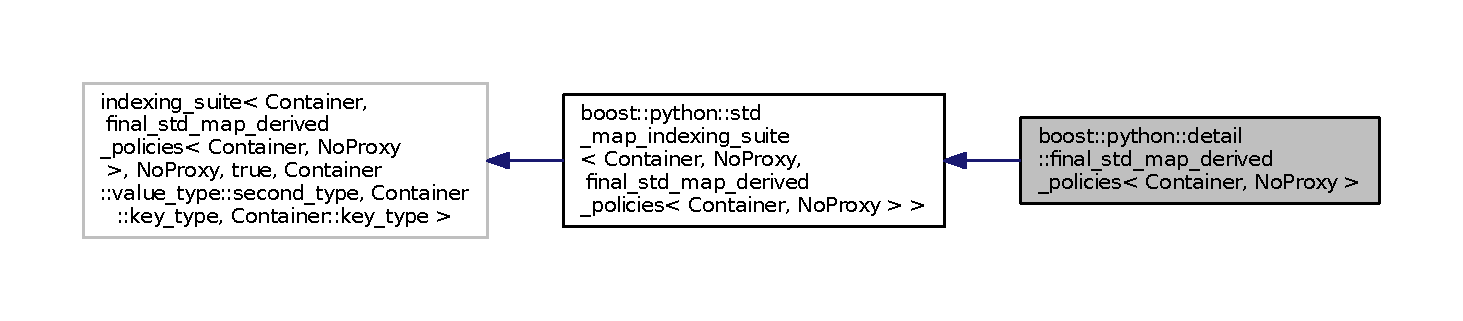
\includegraphics[width=350pt]{classboost_1_1python_1_1detail_1_1final__std__map__derived__policies__coll__graph}
\end{center}
\end{figure}
\subsection*{Additional Inherited Members}


The documentation for this class was generated from the following file\+:\begin{DoxyCompactItemize}
\item 
/home/vrabaud/workspace/recognition\+\_\+kitchen/src/ecto/include/ecto/python/\hyperlink{std__map__indexing__suite_8hpp}{std\+\_\+map\+\_\+indexing\+\_\+suite.\+hpp}\end{DoxyCompactItemize}

\hypertarget{classboost_1_1python_1_1detail_1_1final__std__vector__derived__policies}{}\section{boost\+:\+:python\+:\+:detail\+:\+:final\+\_\+std\+\_\+vector\+\_\+derived\+\_\+policies$<$ Container, No\+Proxy $>$ Class Template Reference}
\label{classboost_1_1python_1_1detail_1_1final__std__vector__derived__policies}\index{boost\+::python\+::detail\+::final\+\_\+std\+\_\+vector\+\_\+derived\+\_\+policies$<$ Container, No\+Proxy $>$@{boost\+::python\+::detail\+::final\+\_\+std\+\_\+vector\+\_\+derived\+\_\+policies$<$ Container, No\+Proxy $>$}}


{\ttfamily \#include $<$std\+\_\+vector\+\_\+indexing\+\_\+suite.\+hpp$>$}



Inheritance diagram for boost\+:\+:python\+:\+:detail\+:\+:final\+\_\+std\+\_\+vector\+\_\+derived\+\_\+policies$<$ Container, No\+Proxy $>$\+:\nopagebreak
\begin{figure}[H]
\begin{center}
\leavevmode
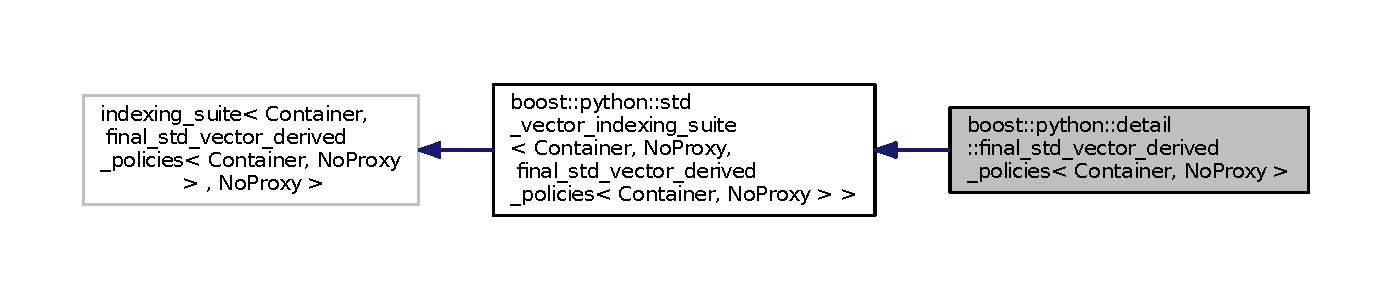
\includegraphics[width=350pt]{classboost_1_1python_1_1detail_1_1final__std__vector__derived__policies__inherit__graph}
\end{center}
\end{figure}


Collaboration diagram for boost\+:\+:python\+:\+:detail\+:\+:final\+\_\+std\+\_\+vector\+\_\+derived\+\_\+policies$<$ Container, No\+Proxy $>$\+:\nopagebreak
\begin{figure}[H]
\begin{center}
\leavevmode
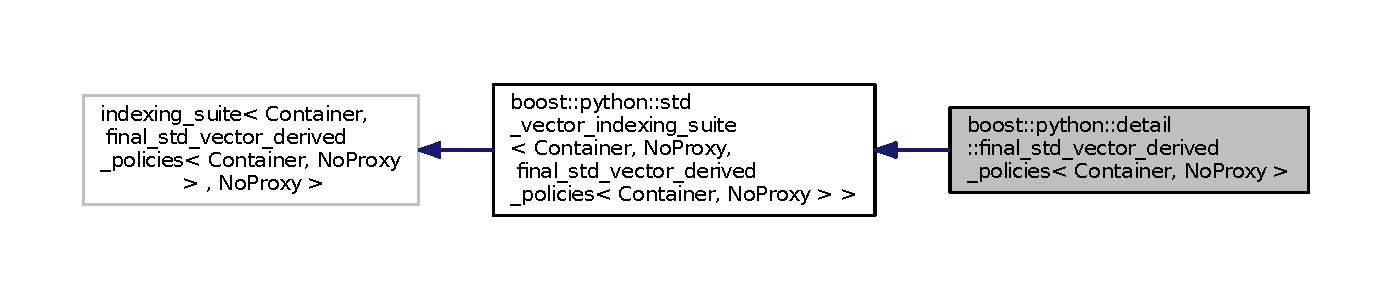
\includegraphics[width=350pt]{classboost_1_1python_1_1detail_1_1final__std__vector__derived__policies__coll__graph}
\end{center}
\end{figure}
\subsection*{Additional Inherited Members}


The documentation for this class was generated from the following file\+:\begin{DoxyCompactItemize}
\item 
/home/vrabaud/workspace/recognition\+\_\+kitchen/src/ecto/include/ecto/python/\hyperlink{std__vector__indexing__suite_8hpp}{std\+\_\+vector\+\_\+indexing\+\_\+suite.\+hpp}\end{DoxyCompactItemize}

\hypertarget{classecto_1_1py_1_1gil}{\section{ecto\-:\-:py\-:\-:gil Class Reference}
\label{classecto_1_1py_1_1gil}\index{ecto\-::py\-::gil@{ecto\-::py\-::gil}}
}


{\ttfamily \#include $<$gil.\-hpp$>$}



Inheritance diagram for ecto\-:\-:py\-:\-:gil\-:\nopagebreak
\begin{figure}[H]
\begin{center}
\leavevmode
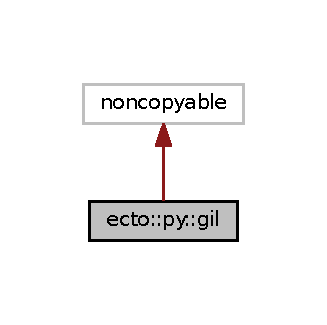
\includegraphics[width=156pt]{classecto_1_1py_1_1gil__inherit__graph}
\end{center}
\end{figure}


Collaboration diagram for ecto\-:\-:py\-:\-:gil\-:\nopagebreak
\begin{figure}[H]
\begin{center}
\leavevmode
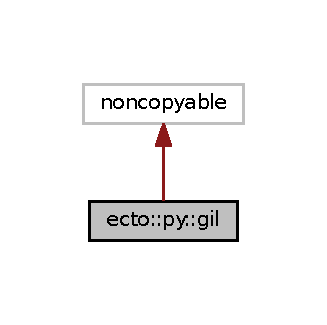
\includegraphics[width=156pt]{classecto_1_1py_1_1gil__coll__graph}
\end{center}
\end{figure}
\subsection*{Public Member Functions}
\begin{DoxyCompactItemize}
\item 
\hyperlink{classecto_1_1py_1_1gil_aad7e0cb610b4766dbdfa918227e806cc}{gil} ()
\item 
\hyperlink{classecto_1_1py_1_1gil_a18685c76c39837ddf90159fb0721ab62}{$\sim$gil} ()
\end{DoxyCompactItemize}
\subsection*{Private Attributes}
\begin{DoxyCompactItemize}
\item 
boost\-::scoped\-\_\-ptr$<$ impl $>$ \hyperlink{classecto_1_1py_1_1gil_af91dedbf0eb88a914bacb64ff176bf93}{impl\-\_\-}
\end{DoxyCompactItemize}


\subsection{Constructor \& Destructor Documentation}
\hypertarget{classecto_1_1py_1_1gil_aad7e0cb610b4766dbdfa918227e806cc}{\index{ecto\-::py\-::gil@{ecto\-::py\-::gil}!gil@{gil}}
\index{gil@{gil}!ecto::py::gil@{ecto\-::py\-::gil}}
\subsubsection[{gil}]{\setlength{\rightskip}{0pt plus 5cm}ecto\-::py\-::gil\-::gil (
\begin{DoxyParamCaption}
{}
\end{DoxyParamCaption}
)}}\label{classecto_1_1py_1_1gil_aad7e0cb610b4766dbdfa918227e806cc}
\hypertarget{classecto_1_1py_1_1gil_a18685c76c39837ddf90159fb0721ab62}{\index{ecto\-::py\-::gil@{ecto\-::py\-::gil}!$\sim$gil@{$\sim$gil}}
\index{$\sim$gil@{$\sim$gil}!ecto::py::gil@{ecto\-::py\-::gil}}
\subsubsection[{$\sim$gil}]{\setlength{\rightskip}{0pt plus 5cm}ecto\-::py\-::gil\-::$\sim$gil (
\begin{DoxyParamCaption}
{}
\end{DoxyParamCaption}
)}}\label{classecto_1_1py_1_1gil_a18685c76c39837ddf90159fb0721ab62}


\subsection{Member Data Documentation}
\hypertarget{classecto_1_1py_1_1gil_af91dedbf0eb88a914bacb64ff176bf93}{\index{ecto\-::py\-::gil@{ecto\-::py\-::gil}!impl\-\_\-@{impl\-\_\-}}
\index{impl\-\_\-@{impl\-\_\-}!ecto::py::gil@{ecto\-::py\-::gil}}
\subsubsection[{impl\-\_\-}]{\setlength{\rightskip}{0pt plus 5cm}boost\-::scoped\-\_\-ptr$<$impl$>$ ecto\-::py\-::gil\-::impl\-\_\-\hspace{0.3cm}{\ttfamily [private]}}}\label{classecto_1_1py_1_1gil_af91dedbf0eb88a914bacb64ff176bf93}


The documentation for this class was generated from the following file\-:\begin{DoxyCompactItemize}
\item 
/home/vrabaud/workspace/recognition\-\_\-kitchen/src/ecto/include/ecto/python/\hyperlink{gil_8hpp}{gil.\-hpp}\end{DoxyCompactItemize}

\hypertarget{structecto_1_1py_1_1gilstatus}{\section{ecto\-:\-:py\-:\-:gilstatus Struct Reference}
\label{structecto_1_1py_1_1gilstatus}\index{ecto\-::py\-::gilstatus@{ecto\-::py\-::gilstatus}}
}


{\ttfamily \#include $<$python.\-hpp$>$}

\subsection*{Public Member Functions}
\begin{DoxyCompactItemize}
\item 
\hyperlink{structecto_1_1py_1_1gilstatus_a9d3fd3fb2c0db89ac667eb534d9ba470}{gilstatus} (const char $\ast$f, unsigned l, const char $\ast$w)
\end{DoxyCompactItemize}
\subsection*{Public Attributes}
\begin{DoxyCompactItemize}
\item 
const char $\ast$ \hyperlink{structecto_1_1py_1_1gilstatus_a454efe188c683788ca52b64b1c87245b}{file}
\item 
unsigned \hyperlink{structecto_1_1py_1_1gilstatus_a86f9f360d4950496f737ce0faa4d7e1b}{line}
\item 
const char $\ast$ \hyperlink{structecto_1_1py_1_1gilstatus_aaeba7e13dad90eaefa0a3c119e0a33ff}{what}
\end{DoxyCompactItemize}


\subsection{Constructor \& Destructor Documentation}
\hypertarget{structecto_1_1py_1_1gilstatus_a9d3fd3fb2c0db89ac667eb534d9ba470}{\index{ecto\-::py\-::gilstatus@{ecto\-::py\-::gilstatus}!gilstatus@{gilstatus}}
\index{gilstatus@{gilstatus}!ecto::py::gilstatus@{ecto\-::py\-::gilstatus}}
\subsubsection[{gilstatus}]{\setlength{\rightskip}{0pt plus 5cm}ecto\-::py\-::gilstatus\-::gilstatus (
\begin{DoxyParamCaption}
\item[{const char $\ast$}]{f, }
\item[{unsigned}]{l, }
\item[{const char $\ast$}]{w}
\end{DoxyParamCaption}
)}}\label{structecto_1_1py_1_1gilstatus_a9d3fd3fb2c0db89ac667eb534d9ba470}


\subsection{Member Data Documentation}
\hypertarget{structecto_1_1py_1_1gilstatus_a454efe188c683788ca52b64b1c87245b}{\index{ecto\-::py\-::gilstatus@{ecto\-::py\-::gilstatus}!file@{file}}
\index{file@{file}!ecto::py::gilstatus@{ecto\-::py\-::gilstatus}}
\subsubsection[{file}]{\setlength{\rightskip}{0pt plus 5cm}const char$\ast$ ecto\-::py\-::gilstatus\-::file}}\label{structecto_1_1py_1_1gilstatus_a454efe188c683788ca52b64b1c87245b}
\hypertarget{structecto_1_1py_1_1gilstatus_a86f9f360d4950496f737ce0faa4d7e1b}{\index{ecto\-::py\-::gilstatus@{ecto\-::py\-::gilstatus}!line@{line}}
\index{line@{line}!ecto::py::gilstatus@{ecto\-::py\-::gilstatus}}
\subsubsection[{line}]{\setlength{\rightskip}{0pt plus 5cm}unsigned ecto\-::py\-::gilstatus\-::line}}\label{structecto_1_1py_1_1gilstatus_a86f9f360d4950496f737ce0faa4d7e1b}
\hypertarget{structecto_1_1py_1_1gilstatus_aaeba7e13dad90eaefa0a3c119e0a33ff}{\index{ecto\-::py\-::gilstatus@{ecto\-::py\-::gilstatus}!what@{what}}
\index{what@{what}!ecto::py::gilstatus@{ecto\-::py\-::gilstatus}}
\subsubsection[{what}]{\setlength{\rightskip}{0pt plus 5cm}const char$\ast$ ecto\-::py\-::gilstatus\-::what}}\label{structecto_1_1py_1_1gilstatus_aaeba7e13dad90eaefa0a3c119e0a33ff}


The documentation for this struct was generated from the following file\-:\begin{DoxyCompactItemize}
\item 
/home/vrabaud/workspace/recognition\-\_\-kitchen/src/ecto/include/ecto/\hyperlink{python_8hpp}{python.\-hpp}\end{DoxyCompactItemize}

\hypertarget{structecto_1_1profile_1_1graph__stats__type}{}\section{ecto\+:\+:profile\+:\+:graph\+\_\+stats\+\_\+type Struct Reference}
\label{structecto_1_1profile_1_1graph__stats__type}\index{ecto\+::profile\+::graph\+\_\+stats\+\_\+type@{ecto\+::profile\+::graph\+\_\+stats\+\_\+type}}


{\ttfamily \#include $<$profile.\+hpp$>$}

\subsection*{Public Member Functions}
\begin{DoxyCompactItemize}
\item 
\hyperlink{structecto_1_1profile_1_1graph__stats__type_aefc20d119cb949420bf74e845a8a1e8c}{graph\+\_\+stats\+\_\+type} ()
\item 
std\+::string \hyperlink{structecto_1_1profile_1_1graph__stats__type_ab412a3b91cbd9b062cdcd0f078ca163d}{as\+\_\+string} (\hyperlink{structecto_1_1graph_1_1graph__t}{graph\+::graph\+\_\+t} \&g) const 
\end{DoxyCompactItemize}
\subsection*{Public Attributes}
\begin{DoxyCompactItemize}
\item 
boost\+::posix\+\_\+time\+::time\+\_\+duration \hyperlink{structecto_1_1profile_1_1graph__stats__type_a340d79ae72ca5639e55098c860640ba8}{cumulative\+\_\+time}
\item 
uint64\+\_\+t \hyperlink{structecto_1_1profile_1_1graph__stats__type_a0d465d23569a8af1789c0b57ccb21017}{cumulative\+\_\+ticks}
\end{DoxyCompactItemize}


\subsection{Constructor \& Destructor Documentation}
\hypertarget{structecto_1_1profile_1_1graph__stats__type_aefc20d119cb949420bf74e845a8a1e8c}{}\index{ecto\+::profile\+::graph\+\_\+stats\+\_\+type@{ecto\+::profile\+::graph\+\_\+stats\+\_\+type}!graph\+\_\+stats\+\_\+type@{graph\+\_\+stats\+\_\+type}}
\index{graph\+\_\+stats\+\_\+type@{graph\+\_\+stats\+\_\+type}!ecto\+::profile\+::graph\+\_\+stats\+\_\+type@{ecto\+::profile\+::graph\+\_\+stats\+\_\+type}}
\subsubsection[{graph\+\_\+stats\+\_\+type}]{\setlength{\rightskip}{0pt plus 5cm}ecto\+::profile\+::graph\+\_\+stats\+\_\+type\+::graph\+\_\+stats\+\_\+type (
\begin{DoxyParamCaption}
{}
\end{DoxyParamCaption}
)\hspace{0.3cm}{\ttfamily [inline]}}\label{structecto_1_1profile_1_1graph__stats__type_aefc20d119cb949420bf74e845a8a1e8c}


\subsection{Member Function Documentation}
\hypertarget{structecto_1_1profile_1_1graph__stats__type_ab412a3b91cbd9b062cdcd0f078ca163d}{}\index{ecto\+::profile\+::graph\+\_\+stats\+\_\+type@{ecto\+::profile\+::graph\+\_\+stats\+\_\+type}!as\+\_\+string@{as\+\_\+string}}
\index{as\+\_\+string@{as\+\_\+string}!ecto\+::profile\+::graph\+\_\+stats\+\_\+type@{ecto\+::profile\+::graph\+\_\+stats\+\_\+type}}
\subsubsection[{as\+\_\+string}]{\setlength{\rightskip}{0pt plus 5cm}std\+::string ecto\+::profile\+::graph\+\_\+stats\+\_\+type\+::as\+\_\+string (
\begin{DoxyParamCaption}
\item[{{\bf graph\+::graph\+\_\+t} \&}]{g}
\end{DoxyParamCaption}
) const}\label{structecto_1_1profile_1_1graph__stats__type_ab412a3b91cbd9b062cdcd0f078ca163d}


\subsection{Member Data Documentation}
\hypertarget{structecto_1_1profile_1_1graph__stats__type_a0d465d23569a8af1789c0b57ccb21017}{}\index{ecto\+::profile\+::graph\+\_\+stats\+\_\+type@{ecto\+::profile\+::graph\+\_\+stats\+\_\+type}!cumulative\+\_\+ticks@{cumulative\+\_\+ticks}}
\index{cumulative\+\_\+ticks@{cumulative\+\_\+ticks}!ecto\+::profile\+::graph\+\_\+stats\+\_\+type@{ecto\+::profile\+::graph\+\_\+stats\+\_\+type}}
\subsubsection[{cumulative\+\_\+ticks}]{\setlength{\rightskip}{0pt plus 5cm}uint64\+\_\+t ecto\+::profile\+::graph\+\_\+stats\+\_\+type\+::cumulative\+\_\+ticks}\label{structecto_1_1profile_1_1graph__stats__type_a0d465d23569a8af1789c0b57ccb21017}
\hypertarget{structecto_1_1profile_1_1graph__stats__type_a340d79ae72ca5639e55098c860640ba8}{}\index{ecto\+::profile\+::graph\+\_\+stats\+\_\+type@{ecto\+::profile\+::graph\+\_\+stats\+\_\+type}!cumulative\+\_\+time@{cumulative\+\_\+time}}
\index{cumulative\+\_\+time@{cumulative\+\_\+time}!ecto\+::profile\+::graph\+\_\+stats\+\_\+type@{ecto\+::profile\+::graph\+\_\+stats\+\_\+type}}
\subsubsection[{cumulative\+\_\+time}]{\setlength{\rightskip}{0pt plus 5cm}boost\+::posix\+\_\+time\+::time\+\_\+duration ecto\+::profile\+::graph\+\_\+stats\+\_\+type\+::cumulative\+\_\+time}\label{structecto_1_1profile_1_1graph__stats__type_a340d79ae72ca5639e55098c860640ba8}


The documentation for this struct was generated from the following file\+:\begin{DoxyCompactItemize}
\item 
/home/vrabaud/workspace/recognition\+\_\+kitchen/src/ecto/include/ecto/\hyperlink{profile_8hpp}{profile.\+hpp}\end{DoxyCompactItemize}

\hypertarget{structecto_1_1graph_1_1graph__t}{}\section{ecto\+:\+:graph\+:\+:graph\+\_\+t Struct Reference}
\label{structecto_1_1graph_1_1graph__t}\index{ecto\+::graph\+::graph\+\_\+t@{ecto\+::graph\+::graph\+\_\+t}}


{\ttfamily \#include $<$types.\+hpp$>$}



Inheritance diagram for ecto\+:\+:graph\+:\+:graph\+\_\+t\+:\nopagebreak
\begin{figure}[H]
\begin{center}
\leavevmode
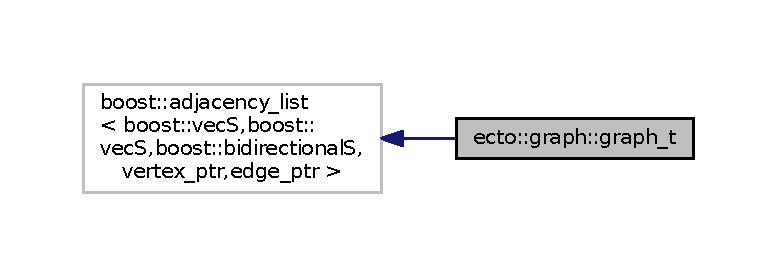
\includegraphics[width=350pt]{structecto_1_1graph_1_1graph__t__inherit__graph}
\end{center}
\end{figure}


Collaboration diagram for ecto\+:\+:graph\+:\+:graph\+\_\+t\+:\nopagebreak
\begin{figure}[H]
\begin{center}
\leavevmode
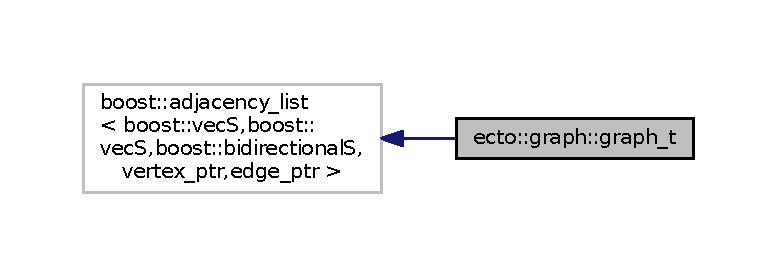
\includegraphics[width=350pt]{structecto_1_1graph_1_1graph__t__coll__graph}
\end{center}
\end{figure}


The documentation for this struct was generated from the following file\+:\begin{DoxyCompactItemize}
\item 
/home/vrabaud/workspace/recognition\+\_\+kitchen/src/ecto/include/ecto/graph/\hyperlink{types_8hpp}{types.\+hpp}\end{DoxyCompactItemize}

\hypertarget{structecto_1_1profile_1_1graphstats__collector}{\section{ecto\-:\-:profile\-:\-:graphstats\-\_\-collector Struct Reference}
\label{structecto_1_1profile_1_1graphstats__collector}\index{ecto\-::profile\-::graphstats\-\_\-collector@{ecto\-::profile\-::graphstats\-\_\-collector}}
}


{\ttfamily \#include $<$profile.\-hpp$>$}



Collaboration diagram for ecto\-:\-:profile\-:\-:graphstats\-\_\-collector\-:\nopagebreak
\begin{figure}[H]
\begin{center}
\leavevmode
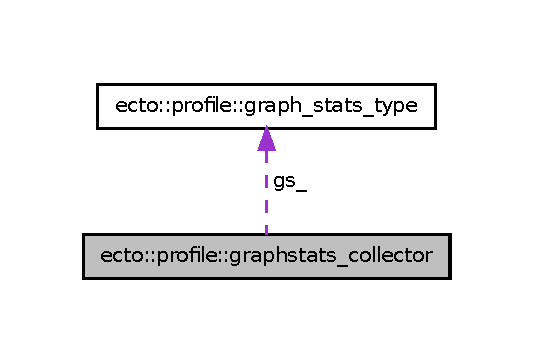
\includegraphics[width=210pt]{structecto_1_1profile_1_1graphstats__collector__coll__graph}
\end{center}
\end{figure}
\subsection*{Public Member Functions}
\begin{DoxyCompactItemize}
\item 
\hyperlink{structecto_1_1profile_1_1graphstats__collector_a375c75ce1c0197d1d87a5fc1bdf97050}{graphstats\-\_\-collector} (\hyperlink{structecto_1_1profile_1_1graph__stats__type}{graph\-\_\-stats\-\_\-type} \&gs)
\item 
\hyperlink{structecto_1_1profile_1_1graphstats__collector_a1bc967dcde1e3418aeeb10e58a52d79f}{$\sim$graphstats\-\_\-collector} ()
\item 
\hyperlink{structecto_1_1profile_1_1graphstats__collector_a375c75ce1c0197d1d87a5fc1bdf97050}{graphstats\-\_\-collector} (\hyperlink{structecto_1_1profile_1_1graph__stats__type}{graph\-\_\-stats\-\_\-type} \&gs)
\item 
\hyperlink{structecto_1_1profile_1_1graphstats__collector_a1bc967dcde1e3418aeeb10e58a52d79f}{$\sim$graphstats\-\_\-collector} ()
\end{DoxyCompactItemize}
\subsection*{Public Attributes}
\begin{DoxyCompactItemize}
\item 
\hyperlink{structecto_1_1profile_1_1graph__stats__type}{graph\-\_\-stats\-\_\-type} \& \hyperlink{structecto_1_1profile_1_1graphstats__collector_ad2a745e661114e28bd044844bf2b60fd}{gs\-\_\-}
\item 
const boost\-::posix\-\_\-time\-::ptime \hyperlink{structecto_1_1profile_1_1graphstats__collector_a85cb67d72c9d1072634b879776e2e4b8}{start\-\_\-time}
\item 
const unsigned long \hyperlink{structecto_1_1profile_1_1graphstats__collector_a7a840b075fd490da5107ea538614d017}{start\-\_\-tick}
\end{DoxyCompactItemize}


\subsection{Constructor \& Destructor Documentation}
\hypertarget{structecto_1_1profile_1_1graphstats__collector_a375c75ce1c0197d1d87a5fc1bdf97050}{\index{ecto\-::profile\-::graphstats\-\_\-collector@{ecto\-::profile\-::graphstats\-\_\-collector}!graphstats\-\_\-collector@{graphstats\-\_\-collector}}
\index{graphstats\-\_\-collector@{graphstats\-\_\-collector}!ecto::profile::graphstats_collector@{ecto\-::profile\-::graphstats\-\_\-collector}}
\subsubsection[{graphstats\-\_\-collector}]{\setlength{\rightskip}{0pt plus 5cm}ecto\-::profile\-::graphstats\-\_\-collector\-::graphstats\-\_\-collector (
\begin{DoxyParamCaption}
\item[{{\bf graph\-\_\-stats\-\_\-type} \&}]{gs}
\end{DoxyParamCaption}
)\hspace{0.3cm}{\ttfamily [inline]}}}\label{structecto_1_1profile_1_1graphstats__collector_a375c75ce1c0197d1d87a5fc1bdf97050}
\hypertarget{structecto_1_1profile_1_1graphstats__collector_a1bc967dcde1e3418aeeb10e58a52d79f}{\index{ecto\-::profile\-::graphstats\-\_\-collector@{ecto\-::profile\-::graphstats\-\_\-collector}!$\sim$graphstats\-\_\-collector@{$\sim$graphstats\-\_\-collector}}
\index{$\sim$graphstats\-\_\-collector@{$\sim$graphstats\-\_\-collector}!ecto::profile::graphstats_collector@{ecto\-::profile\-::graphstats\-\_\-collector}}
\subsubsection[{$\sim$graphstats\-\_\-collector}]{\setlength{\rightskip}{0pt plus 5cm}ecto\-::profile\-::graphstats\-\_\-collector\-::$\sim$graphstats\-\_\-collector (
\begin{DoxyParamCaption}
{}
\end{DoxyParamCaption}
)\hspace{0.3cm}{\ttfamily [inline]}}}\label{structecto_1_1profile_1_1graphstats__collector_a1bc967dcde1e3418aeeb10e58a52d79f}
\hypertarget{structecto_1_1profile_1_1graphstats__collector_a375c75ce1c0197d1d87a5fc1bdf97050}{\index{ecto\-::profile\-::graphstats\-\_\-collector@{ecto\-::profile\-::graphstats\-\_\-collector}!graphstats\-\_\-collector@{graphstats\-\_\-collector}}
\index{graphstats\-\_\-collector@{graphstats\-\_\-collector}!ecto::profile::graphstats_collector@{ecto\-::profile\-::graphstats\-\_\-collector}}
\subsubsection[{graphstats\-\_\-collector}]{\setlength{\rightskip}{0pt plus 5cm}ecto\-::profile\-::graphstats\-\_\-collector\-::graphstats\-\_\-collector (
\begin{DoxyParamCaption}
\item[{{\bf graph\-\_\-stats\-\_\-type} \&}]{gs}
\end{DoxyParamCaption}
)\hspace{0.3cm}{\ttfamily [inline]}}}\label{structecto_1_1profile_1_1graphstats__collector_a375c75ce1c0197d1d87a5fc1bdf97050}
\hypertarget{structecto_1_1profile_1_1graphstats__collector_a1bc967dcde1e3418aeeb10e58a52d79f}{\index{ecto\-::profile\-::graphstats\-\_\-collector@{ecto\-::profile\-::graphstats\-\_\-collector}!$\sim$graphstats\-\_\-collector@{$\sim$graphstats\-\_\-collector}}
\index{$\sim$graphstats\-\_\-collector@{$\sim$graphstats\-\_\-collector}!ecto::profile::graphstats_collector@{ecto\-::profile\-::graphstats\-\_\-collector}}
\subsubsection[{$\sim$graphstats\-\_\-collector}]{\setlength{\rightskip}{0pt plus 5cm}ecto\-::profile\-::graphstats\-\_\-collector\-::$\sim$graphstats\-\_\-collector (
\begin{DoxyParamCaption}
{}
\end{DoxyParamCaption}
)\hspace{0.3cm}{\ttfamily [inline]}}}\label{structecto_1_1profile_1_1graphstats__collector_a1bc967dcde1e3418aeeb10e58a52d79f}


\subsection{Member Data Documentation}
\hypertarget{structecto_1_1profile_1_1graphstats__collector_ad2a745e661114e28bd044844bf2b60fd}{\index{ecto\-::profile\-::graphstats\-\_\-collector@{ecto\-::profile\-::graphstats\-\_\-collector}!gs\-\_\-@{gs\-\_\-}}
\index{gs\-\_\-@{gs\-\_\-}!ecto::profile::graphstats_collector@{ecto\-::profile\-::graphstats\-\_\-collector}}
\subsubsection[{gs\-\_\-}]{\setlength{\rightskip}{0pt plus 5cm}{\bf graph\-\_\-stats\-\_\-type} \& ecto\-::profile\-::graphstats\-\_\-collector\-::gs\-\_\-}}\label{structecto_1_1profile_1_1graphstats__collector_ad2a745e661114e28bd044844bf2b60fd}
\hypertarget{structecto_1_1profile_1_1graphstats__collector_a7a840b075fd490da5107ea538614d017}{\index{ecto\-::profile\-::graphstats\-\_\-collector@{ecto\-::profile\-::graphstats\-\_\-collector}!start\-\_\-tick@{start\-\_\-tick}}
\index{start\-\_\-tick@{start\-\_\-tick}!ecto::profile::graphstats_collector@{ecto\-::profile\-::graphstats\-\_\-collector}}
\subsubsection[{start\-\_\-tick}]{\setlength{\rightskip}{0pt plus 5cm}const unsigned long ecto\-::profile\-::graphstats\-\_\-collector\-::start\-\_\-tick}}\label{structecto_1_1profile_1_1graphstats__collector_a7a840b075fd490da5107ea538614d017}
\hypertarget{structecto_1_1profile_1_1graphstats__collector_a85cb67d72c9d1072634b879776e2e4b8}{\index{ecto\-::profile\-::graphstats\-\_\-collector@{ecto\-::profile\-::graphstats\-\_\-collector}!start\-\_\-time@{start\-\_\-time}}
\index{start\-\_\-time@{start\-\_\-time}!ecto::profile::graphstats_collector@{ecto\-::profile\-::graphstats\-\_\-collector}}
\subsubsection[{start\-\_\-time}]{\setlength{\rightskip}{0pt plus 5cm}const boost\-::posix\-\_\-time\-::ptime ecto\-::profile\-::graphstats\-\_\-collector\-::start\-\_\-time}}\label{structecto_1_1profile_1_1graphstats__collector_a85cb67d72c9d1072634b879776e2e4b8}


The documentation for this struct was generated from the following files\-:\begin{DoxyCompactItemize}
\item 
/home/vrabaud/workspace/recognition\-\_\-kitchen/src/ecto/include/ecto/\hyperlink{profile_8hpp}{profile.\-hpp}\item 
/home/vrabaud/workspace/recognition\-\_\-kitchen/src/ecto/include/ecto/\hyperlink{profile_8hpp~}{profile.\-hpp$\sim$}\end{DoxyCompactItemize}

\hypertarget{structecto_1_1has__f}{}\section{ecto\+:\+:has\+\_\+f$<$ T $>$ Struct Template Reference}
\label{structecto_1_1has__f}\index{ecto\+::has\+\_\+f$<$ T $>$@{ecto\+::has\+\_\+f$<$ T $>$}}


Helper class for determining if client modules have function implementations or not.  




{\ttfamily \#include $<$cell.\+hpp$>$}

\subsection*{Public Types}
\begin{DoxyCompactItemize}
\item 
enum \{ \hyperlink{structecto_1_1has__f_a37dd9c69c6cfed2ac70c2529d493d410a41824f56b5af096de7e6ee2ccbe9943b}{declare\+\_\+params} = sizeof(test\+\_\+declare\+\_\+params$<$T$>$ (0)) == sizeof(yes)
 \}
\item 
enum \{ \hyperlink{structecto_1_1has__f_abc0a1a04163d85af95636c6213729909ac01ab4ed00f005d55b0813ccb49166f2}{declare\+\_\+io} = sizeof(test\+\_\+declare\+\_\+io$<$T$>$ (0)) == sizeof(yes)
 \}
\item 
enum \{ \hyperlink{structecto_1_1has__f_a173737354c871f8785a6bbe7640bda1da1bc6475abb988c1b998c700d66894960}{configure} = sizeof(test\+\_\+configure$<$T$>$ (0)) == sizeof(yes)
 \}
\item 
enum \{ \hyperlink{structecto_1_1has__f_a8f077b20e8dd579e1a427ac6c80c3d3fa848797161f1dda4f3676f4e2271ebe40}{activate} = sizeof(test\+\_\+activate$<$T$>$ (0)) == sizeof(yes)
 \}
\item 
enum \{ \hyperlink{structecto_1_1has__f_afa9dc8feb074d51ee4600f20447b2724a0f0eba1c7cf0a59268313a95842a7b42}{deactivate} = sizeof(test\+\_\+deactivate$<$T$>$ (0)) == sizeof(yes)
 \}
\item 
enum \{ \hyperlink{structecto_1_1has__f_a575b2f80b107061801e4c2ebd36bd2fcaa6d57b41a7edff0b538fbfddd6e1bf0e}{process} = sizeof(test\+\_\+process$<$T$>$ (0)) == sizeof(yes)
 \}
\item 
enum \{ \hyperlink{structecto_1_1has__f_a2f5a531214c34e93b8efd059afed9348a210df924551c3e6407abe7c1f12b85d0}{start} = sizeof(test\+\_\+start$<$T$>$ (0)) == sizeof(yes)
 \}
\item 
enum \{ \hyperlink{structecto_1_1has__f_af1ab6e8ed499c6c3b404cd7aeda85c87a6db3f78bcdda21cf158666ed1f9dfead}{stop} = sizeof(test\+\_\+stop$<$T$>$ (0)) == sizeof(yes)
 \}
\item 
typedef char \hyperlink{structecto_1_1has__f_a3fb902f1eed02919195aff1a6b28eb76}{yes}
\item 
typedef char(\& \hyperlink{structecto_1_1has__f_ae0c6da775cf20caed616e24681af2807}{no})\mbox{[}2\mbox{]}
\end{DoxyCompactItemize}
\subsection*{Static Public Member Functions}
\begin{DoxyCompactItemize}
\item 
{\footnotesize template$<$class U $>$ }\\static \hyperlink{structecto_1_1has__f_a3fb902f1eed02919195aff1a6b28eb76}{yes} \hyperlink{structecto_1_1has__f_ae63216bd7936dc02af86363f8db74b2e}{test\+\_\+declare\+\_\+params} (\+\_\+\+\_\+typeof\+\_\+\+\_\+(\&U\+::declare\+\_\+params))
\item 
{\footnotesize template$<$class U $>$ }\\static \hyperlink{structecto_1_1has__f_ae0c6da775cf20caed616e24681af2807}{no} \hyperlink{structecto_1_1has__f_ab2f2693b1d6084a672893777893b9ab2}{test\+\_\+declare\+\_\+params} (...)
\item 
{\footnotesize template$<$class U $>$ }\\static \hyperlink{structecto_1_1has__f_a3fb902f1eed02919195aff1a6b28eb76}{yes} \hyperlink{structecto_1_1has__f_a042de0d066c5b000186594964deea94e}{test\+\_\+declare\+\_\+io} (\+\_\+\+\_\+typeof\+\_\+\+\_\+(\&U\+::declare\+\_\+io))
\item 
{\footnotesize template$<$class U $>$ }\\static \hyperlink{structecto_1_1has__f_ae0c6da775cf20caed616e24681af2807}{no} \hyperlink{structecto_1_1has__f_ad144a46699c480e7851fbd36394a1fe3}{test\+\_\+declare\+\_\+io} (...)
\item 
{\footnotesize template$<$class U $>$ }\\static \hyperlink{structecto_1_1has__f_a3fb902f1eed02919195aff1a6b28eb76}{yes} \hyperlink{structecto_1_1has__f_a6665bfebbc796527bc1a775803ebd18e}{test\+\_\+configure} (\+\_\+\+\_\+typeof\+\_\+\+\_\+(\&U\+::configure))
\item 
{\footnotesize template$<$class U $>$ }\\static \hyperlink{structecto_1_1has__f_ae0c6da775cf20caed616e24681af2807}{no} \hyperlink{structecto_1_1has__f_afc5065e1043ffe865662840f3a9d82fd}{test\+\_\+configure} (...)
\item 
{\footnotesize template$<$class U $>$ }\\static \hyperlink{structecto_1_1has__f_a3fb902f1eed02919195aff1a6b28eb76}{yes} \hyperlink{structecto_1_1has__f_a2212643cf55b3264654bc654df699cb7}{test\+\_\+activate} (\+\_\+\+\_\+typeof\+\_\+\+\_\+(\&U\+::activate))
\item 
{\footnotesize template$<$class U $>$ }\\static \hyperlink{structecto_1_1has__f_ae0c6da775cf20caed616e24681af2807}{no} \hyperlink{structecto_1_1has__f_a2f43dbf6bee3d172c280f00e8fe73c33}{test\+\_\+activate} (...)
\item 
{\footnotesize template$<$class U $>$ }\\static \hyperlink{structecto_1_1has__f_a3fb902f1eed02919195aff1a6b28eb76}{yes} \hyperlink{structecto_1_1has__f_ae924c11bc0462d832fdd8ea97bd3599d}{test\+\_\+deactivate} (\+\_\+\+\_\+typeof\+\_\+\+\_\+(\&U\+::deactivate))
\item 
{\footnotesize template$<$class U $>$ }\\static \hyperlink{structecto_1_1has__f_ae0c6da775cf20caed616e24681af2807}{no} \hyperlink{structecto_1_1has__f_ab8c699587d6f7d476d09b693227f5373}{test\+\_\+deactivate} (...)
\item 
{\footnotesize template$<$class U $>$ }\\static \hyperlink{structecto_1_1has__f_a3fb902f1eed02919195aff1a6b28eb76}{yes} \hyperlink{structecto_1_1has__f_a4e6f5942e9ee41196b52f7c728baf547}{test\+\_\+process} (\+\_\+\+\_\+typeof\+\_\+\+\_\+(\&U\+::process))
\item 
{\footnotesize template$<$class U $>$ }\\static \hyperlink{structecto_1_1has__f_ae0c6da775cf20caed616e24681af2807}{no} \hyperlink{structecto_1_1has__f_a75ec2b3763995883f3a5dd1b19097439}{test\+\_\+process} (...)
\item 
{\footnotesize template$<$class U $>$ }\\static \hyperlink{structecto_1_1has__f_a3fb902f1eed02919195aff1a6b28eb76}{yes} \hyperlink{structecto_1_1has__f_aa88ebe0fd23a4e875704da0d62ce489c}{test\+\_\+start} (\+\_\+\+\_\+typeof\+\_\+\+\_\+(\&U\+::start))
\item 
{\footnotesize template$<$class U $>$ }\\static \hyperlink{structecto_1_1has__f_ae0c6da775cf20caed616e24681af2807}{no} \hyperlink{structecto_1_1has__f_a089044f39fac5f7ea53eec64799c4619}{test\+\_\+start} (...)
\item 
{\footnotesize template$<$class U $>$ }\\static \hyperlink{structecto_1_1has__f_a3fb902f1eed02919195aff1a6b28eb76}{yes} \hyperlink{structecto_1_1has__f_a4de2275b91096c6e6d1efc2f137c380f}{test\+\_\+stop} (\+\_\+\+\_\+typeof\+\_\+\+\_\+(\&U\+::stop))
\item 
{\footnotesize template$<$class U $>$ }\\static \hyperlink{structecto_1_1has__f_ae0c6da775cf20caed616e24681af2807}{no} \hyperlink{structecto_1_1has__f_a97d550e44f5260b40ddd0722bdd6f274}{test\+\_\+stop} (...)
\end{DoxyCompactItemize}


\subsection{Detailed Description}
\subsubsection*{template$<$class T$>$struct ecto\+::has\+\_\+f$<$ T $>$}

Helper class for determining if client modules have function implementations or not. 

\subsection{Member Typedef Documentation}
\hypertarget{structecto_1_1has__f_ae0c6da775cf20caed616e24681af2807}{}\index{ecto\+::has\+\_\+f@{ecto\+::has\+\_\+f}!no@{no}}
\index{no@{no}!ecto\+::has\+\_\+f@{ecto\+::has\+\_\+f}}
\subsubsection[{no}]{\setlength{\rightskip}{0pt plus 5cm}template$<$class T $>$ typedef char(\& {\bf ecto\+::has\+\_\+f}$<$ T $>$\+::no)\mbox{[}2\mbox{]}}\label{structecto_1_1has__f_ae0c6da775cf20caed616e24681af2807}
\hypertarget{structecto_1_1has__f_a3fb902f1eed02919195aff1a6b28eb76}{}\index{ecto\+::has\+\_\+f@{ecto\+::has\+\_\+f}!yes@{yes}}
\index{yes@{yes}!ecto\+::has\+\_\+f@{ecto\+::has\+\_\+f}}
\subsubsection[{yes}]{\setlength{\rightskip}{0pt plus 5cm}template$<$class T $>$ typedef char {\bf ecto\+::has\+\_\+f}$<$ T $>$\+::{\bf yes}}\label{structecto_1_1has__f_a3fb902f1eed02919195aff1a6b28eb76}


\subsection{Member Enumeration Documentation}
\hypertarget{structecto_1_1has__f_a37dd9c69c6cfed2ac70c2529d493d410}{}\subsubsection[{anonymous enum}]{\setlength{\rightskip}{0pt plus 5cm}template$<$class T $>$ anonymous enum}\label{structecto_1_1has__f_a37dd9c69c6cfed2ac70c2529d493d410}
\begin{Desc}
\item[Enumerator]\par
\begin{description}
\index{declare\+\_\+params@{declare\+\_\+params}!ecto\+::has\+\_\+f@{ecto\+::has\+\_\+f}}\index{ecto\+::has\+\_\+f@{ecto\+::has\+\_\+f}!declare\+\_\+params@{declare\+\_\+params}}\item[{\em 
\hypertarget{structecto_1_1has__f_a37dd9c69c6cfed2ac70c2529d493d410a41824f56b5af096de7e6ee2ccbe9943b}{}declare\+\_\+params\label{structecto_1_1has__f_a37dd9c69c6cfed2ac70c2529d493d410a41824f56b5af096de7e6ee2ccbe9943b}
}]\end{description}
\end{Desc}
\hypertarget{structecto_1_1has__f_abc0a1a04163d85af95636c6213729909}{}\subsubsection[{anonymous enum}]{\setlength{\rightskip}{0pt plus 5cm}template$<$class T $>$ anonymous enum}\label{structecto_1_1has__f_abc0a1a04163d85af95636c6213729909}
\begin{Desc}
\item[Enumerator]\par
\begin{description}
\index{declare\+\_\+io@{declare\+\_\+io}!ecto\+::has\+\_\+f@{ecto\+::has\+\_\+f}}\index{ecto\+::has\+\_\+f@{ecto\+::has\+\_\+f}!declare\+\_\+io@{declare\+\_\+io}}\item[{\em 
\hypertarget{structecto_1_1has__f_abc0a1a04163d85af95636c6213729909ac01ab4ed00f005d55b0813ccb49166f2}{}declare\+\_\+io\label{structecto_1_1has__f_abc0a1a04163d85af95636c6213729909ac01ab4ed00f005d55b0813ccb49166f2}
}]\end{description}
\end{Desc}
\hypertarget{structecto_1_1has__f_a173737354c871f8785a6bbe7640bda1d}{}\subsubsection[{anonymous enum}]{\setlength{\rightskip}{0pt plus 5cm}template$<$class T $>$ anonymous enum}\label{structecto_1_1has__f_a173737354c871f8785a6bbe7640bda1d}
\begin{Desc}
\item[Enumerator]\par
\begin{description}
\index{configure@{configure}!ecto\+::has\+\_\+f@{ecto\+::has\+\_\+f}}\index{ecto\+::has\+\_\+f@{ecto\+::has\+\_\+f}!configure@{configure}}\item[{\em 
\hypertarget{structecto_1_1has__f_a173737354c871f8785a6bbe7640bda1da1bc6475abb988c1b998c700d66894960}{}configure\label{structecto_1_1has__f_a173737354c871f8785a6bbe7640bda1da1bc6475abb988c1b998c700d66894960}
}]\end{description}
\end{Desc}
\hypertarget{structecto_1_1has__f_a8f077b20e8dd579e1a427ac6c80c3d3f}{}\subsubsection[{anonymous enum}]{\setlength{\rightskip}{0pt plus 5cm}template$<$class T $>$ anonymous enum}\label{structecto_1_1has__f_a8f077b20e8dd579e1a427ac6c80c3d3f}
\begin{Desc}
\item[Enumerator]\par
\begin{description}
\index{activate@{activate}!ecto\+::has\+\_\+f@{ecto\+::has\+\_\+f}}\index{ecto\+::has\+\_\+f@{ecto\+::has\+\_\+f}!activate@{activate}}\item[{\em 
\hypertarget{structecto_1_1has__f_a8f077b20e8dd579e1a427ac6c80c3d3fa848797161f1dda4f3676f4e2271ebe40}{}activate\label{structecto_1_1has__f_a8f077b20e8dd579e1a427ac6c80c3d3fa848797161f1dda4f3676f4e2271ebe40}
}]\end{description}
\end{Desc}
\hypertarget{structecto_1_1has__f_afa9dc8feb074d51ee4600f20447b2724}{}\subsubsection[{anonymous enum}]{\setlength{\rightskip}{0pt plus 5cm}template$<$class T $>$ anonymous enum}\label{structecto_1_1has__f_afa9dc8feb074d51ee4600f20447b2724}
\begin{Desc}
\item[Enumerator]\par
\begin{description}
\index{deactivate@{deactivate}!ecto\+::has\+\_\+f@{ecto\+::has\+\_\+f}}\index{ecto\+::has\+\_\+f@{ecto\+::has\+\_\+f}!deactivate@{deactivate}}\item[{\em 
\hypertarget{structecto_1_1has__f_afa9dc8feb074d51ee4600f20447b2724a0f0eba1c7cf0a59268313a95842a7b42}{}deactivate\label{structecto_1_1has__f_afa9dc8feb074d51ee4600f20447b2724a0f0eba1c7cf0a59268313a95842a7b42}
}]\end{description}
\end{Desc}
\hypertarget{structecto_1_1has__f_a575b2f80b107061801e4c2ebd36bd2fc}{}\subsubsection[{anonymous enum}]{\setlength{\rightskip}{0pt plus 5cm}template$<$class T $>$ anonymous enum}\label{structecto_1_1has__f_a575b2f80b107061801e4c2ebd36bd2fc}
\begin{Desc}
\item[Enumerator]\par
\begin{description}
\index{process@{process}!ecto\+::has\+\_\+f@{ecto\+::has\+\_\+f}}\index{ecto\+::has\+\_\+f@{ecto\+::has\+\_\+f}!process@{process}}\item[{\em 
\hypertarget{structecto_1_1has__f_a575b2f80b107061801e4c2ebd36bd2fcaa6d57b41a7edff0b538fbfddd6e1bf0e}{}process\label{structecto_1_1has__f_a575b2f80b107061801e4c2ebd36bd2fcaa6d57b41a7edff0b538fbfddd6e1bf0e}
}]\end{description}
\end{Desc}
\hypertarget{structecto_1_1has__f_a2f5a531214c34e93b8efd059afed9348}{}\subsubsection[{anonymous enum}]{\setlength{\rightskip}{0pt plus 5cm}template$<$class T $>$ anonymous enum}\label{structecto_1_1has__f_a2f5a531214c34e93b8efd059afed9348}
\begin{Desc}
\item[Enumerator]\par
\begin{description}
\index{start@{start}!ecto\+::has\+\_\+f@{ecto\+::has\+\_\+f}}\index{ecto\+::has\+\_\+f@{ecto\+::has\+\_\+f}!start@{start}}\item[{\em 
\hypertarget{structecto_1_1has__f_a2f5a531214c34e93b8efd059afed9348a210df924551c3e6407abe7c1f12b85d0}{}start\label{structecto_1_1has__f_a2f5a531214c34e93b8efd059afed9348a210df924551c3e6407abe7c1f12b85d0}
}]\end{description}
\end{Desc}
\hypertarget{structecto_1_1has__f_af1ab6e8ed499c6c3b404cd7aeda85c87}{}\subsubsection[{anonymous enum}]{\setlength{\rightskip}{0pt plus 5cm}template$<$class T $>$ anonymous enum}\label{structecto_1_1has__f_af1ab6e8ed499c6c3b404cd7aeda85c87}
\begin{Desc}
\item[Enumerator]\par
\begin{description}
\index{stop@{stop}!ecto\+::has\+\_\+f@{ecto\+::has\+\_\+f}}\index{ecto\+::has\+\_\+f@{ecto\+::has\+\_\+f}!stop@{stop}}\item[{\em 
\hypertarget{structecto_1_1has__f_af1ab6e8ed499c6c3b404cd7aeda85c87a6db3f78bcdda21cf158666ed1f9dfead}{}stop\label{structecto_1_1has__f_af1ab6e8ed499c6c3b404cd7aeda85c87a6db3f78bcdda21cf158666ed1f9dfead}
}]\end{description}
\end{Desc}


\subsection{Member Function Documentation}
\hypertarget{structecto_1_1has__f_a2212643cf55b3264654bc654df699cb7}{}\index{ecto\+::has\+\_\+f@{ecto\+::has\+\_\+f}!test\+\_\+activate@{test\+\_\+activate}}
\index{test\+\_\+activate@{test\+\_\+activate}!ecto\+::has\+\_\+f@{ecto\+::has\+\_\+f}}
\subsubsection[{test\+\_\+activate}]{\setlength{\rightskip}{0pt plus 5cm}template$<$class T $>$ template$<$class U $>$ static {\bf yes} {\bf ecto\+::has\+\_\+f}$<$ T $>$\+::test\+\_\+activate (
\begin{DoxyParamCaption}
\item[{\+\_\+\+\_\+typeof\+\_\+\+\_\+ \&\+::{\bf activate}}]{}
\end{DoxyParamCaption}
)\hspace{0.3cm}{\ttfamily [static]}}\label{structecto_1_1has__f_a2212643cf55b3264654bc654df699cb7}
\hypertarget{structecto_1_1has__f_a2f43dbf6bee3d172c280f00e8fe73c33}{}\index{ecto\+::has\+\_\+f@{ecto\+::has\+\_\+f}!test\+\_\+activate@{test\+\_\+activate}}
\index{test\+\_\+activate@{test\+\_\+activate}!ecto\+::has\+\_\+f@{ecto\+::has\+\_\+f}}
\subsubsection[{test\+\_\+activate}]{\setlength{\rightskip}{0pt plus 5cm}template$<$class T $>$ template$<$class U $>$ static {\bf no} {\bf ecto\+::has\+\_\+f}$<$ T $>$\+::test\+\_\+activate (
\begin{DoxyParamCaption}
\item[{}]{...}
\end{DoxyParamCaption}
)\hspace{0.3cm}{\ttfamily [static]}}\label{structecto_1_1has__f_a2f43dbf6bee3d172c280f00e8fe73c33}
\hypertarget{structecto_1_1has__f_a6665bfebbc796527bc1a775803ebd18e}{}\index{ecto\+::has\+\_\+f@{ecto\+::has\+\_\+f}!test\+\_\+configure@{test\+\_\+configure}}
\index{test\+\_\+configure@{test\+\_\+configure}!ecto\+::has\+\_\+f@{ecto\+::has\+\_\+f}}
\subsubsection[{test\+\_\+configure}]{\setlength{\rightskip}{0pt plus 5cm}template$<$class T $>$ template$<$class U $>$ static {\bf yes} {\bf ecto\+::has\+\_\+f}$<$ T $>$\+::test\+\_\+configure (
\begin{DoxyParamCaption}
\item[{\+\_\+\+\_\+typeof\+\_\+\+\_\+ \&\+::{\bf configure}}]{}
\end{DoxyParamCaption}
)\hspace{0.3cm}{\ttfamily [static]}}\label{structecto_1_1has__f_a6665bfebbc796527bc1a775803ebd18e}
\hypertarget{structecto_1_1has__f_afc5065e1043ffe865662840f3a9d82fd}{}\index{ecto\+::has\+\_\+f@{ecto\+::has\+\_\+f}!test\+\_\+configure@{test\+\_\+configure}}
\index{test\+\_\+configure@{test\+\_\+configure}!ecto\+::has\+\_\+f@{ecto\+::has\+\_\+f}}
\subsubsection[{test\+\_\+configure}]{\setlength{\rightskip}{0pt plus 5cm}template$<$class T $>$ template$<$class U $>$ static {\bf no} {\bf ecto\+::has\+\_\+f}$<$ T $>$\+::test\+\_\+configure (
\begin{DoxyParamCaption}
\item[{}]{...}
\end{DoxyParamCaption}
)\hspace{0.3cm}{\ttfamily [static]}}\label{structecto_1_1has__f_afc5065e1043ffe865662840f3a9d82fd}
\hypertarget{structecto_1_1has__f_ae924c11bc0462d832fdd8ea97bd3599d}{}\index{ecto\+::has\+\_\+f@{ecto\+::has\+\_\+f}!test\+\_\+deactivate@{test\+\_\+deactivate}}
\index{test\+\_\+deactivate@{test\+\_\+deactivate}!ecto\+::has\+\_\+f@{ecto\+::has\+\_\+f}}
\subsubsection[{test\+\_\+deactivate}]{\setlength{\rightskip}{0pt plus 5cm}template$<$class T $>$ template$<$class U $>$ static {\bf yes} {\bf ecto\+::has\+\_\+f}$<$ T $>$\+::test\+\_\+deactivate (
\begin{DoxyParamCaption}
\item[{\+\_\+\+\_\+typeof\+\_\+\+\_\+ \&\+::{\bf deactivate}}]{}
\end{DoxyParamCaption}
)\hspace{0.3cm}{\ttfamily [static]}}\label{structecto_1_1has__f_ae924c11bc0462d832fdd8ea97bd3599d}
\hypertarget{structecto_1_1has__f_ab8c699587d6f7d476d09b693227f5373}{}\index{ecto\+::has\+\_\+f@{ecto\+::has\+\_\+f}!test\+\_\+deactivate@{test\+\_\+deactivate}}
\index{test\+\_\+deactivate@{test\+\_\+deactivate}!ecto\+::has\+\_\+f@{ecto\+::has\+\_\+f}}
\subsubsection[{test\+\_\+deactivate}]{\setlength{\rightskip}{0pt plus 5cm}template$<$class T $>$ template$<$class U $>$ static {\bf no} {\bf ecto\+::has\+\_\+f}$<$ T $>$\+::test\+\_\+deactivate (
\begin{DoxyParamCaption}
\item[{}]{...}
\end{DoxyParamCaption}
)\hspace{0.3cm}{\ttfamily [static]}}\label{structecto_1_1has__f_ab8c699587d6f7d476d09b693227f5373}
\hypertarget{structecto_1_1has__f_a042de0d066c5b000186594964deea94e}{}\index{ecto\+::has\+\_\+f@{ecto\+::has\+\_\+f}!test\+\_\+declare\+\_\+io@{test\+\_\+declare\+\_\+io}}
\index{test\+\_\+declare\+\_\+io@{test\+\_\+declare\+\_\+io}!ecto\+::has\+\_\+f@{ecto\+::has\+\_\+f}}
\subsubsection[{test\+\_\+declare\+\_\+io}]{\setlength{\rightskip}{0pt plus 5cm}template$<$class T $>$ template$<$class U $>$ static {\bf yes} {\bf ecto\+::has\+\_\+f}$<$ T $>$\+::test\+\_\+declare\+\_\+io (
\begin{DoxyParamCaption}
\item[{\+\_\+\+\_\+typeof\+\_\+\+\_\+ \&\+::{\bf declare\+\_\+io}}]{}
\end{DoxyParamCaption}
)\hspace{0.3cm}{\ttfamily [static]}}\label{structecto_1_1has__f_a042de0d066c5b000186594964deea94e}
\hypertarget{structecto_1_1has__f_ad144a46699c480e7851fbd36394a1fe3}{}\index{ecto\+::has\+\_\+f@{ecto\+::has\+\_\+f}!test\+\_\+declare\+\_\+io@{test\+\_\+declare\+\_\+io}}
\index{test\+\_\+declare\+\_\+io@{test\+\_\+declare\+\_\+io}!ecto\+::has\+\_\+f@{ecto\+::has\+\_\+f}}
\subsubsection[{test\+\_\+declare\+\_\+io}]{\setlength{\rightskip}{0pt plus 5cm}template$<$class T $>$ template$<$class U $>$ static {\bf no} {\bf ecto\+::has\+\_\+f}$<$ T $>$\+::test\+\_\+declare\+\_\+io (
\begin{DoxyParamCaption}
\item[{}]{...}
\end{DoxyParamCaption}
)\hspace{0.3cm}{\ttfamily [static]}}\label{structecto_1_1has__f_ad144a46699c480e7851fbd36394a1fe3}
\hypertarget{structecto_1_1has__f_ae63216bd7936dc02af86363f8db74b2e}{}\index{ecto\+::has\+\_\+f@{ecto\+::has\+\_\+f}!test\+\_\+declare\+\_\+params@{test\+\_\+declare\+\_\+params}}
\index{test\+\_\+declare\+\_\+params@{test\+\_\+declare\+\_\+params}!ecto\+::has\+\_\+f@{ecto\+::has\+\_\+f}}
\subsubsection[{test\+\_\+declare\+\_\+params}]{\setlength{\rightskip}{0pt plus 5cm}template$<$class T $>$ template$<$class U $>$ static {\bf yes} {\bf ecto\+::has\+\_\+f}$<$ T $>$\+::test\+\_\+declare\+\_\+params (
\begin{DoxyParamCaption}
\item[{\+\_\+\+\_\+typeof\+\_\+\+\_\+ \&\+::{\bf declare\+\_\+params}}]{}
\end{DoxyParamCaption}
)\hspace{0.3cm}{\ttfamily [static]}}\label{structecto_1_1has__f_ae63216bd7936dc02af86363f8db74b2e}
\hypertarget{structecto_1_1has__f_ab2f2693b1d6084a672893777893b9ab2}{}\index{ecto\+::has\+\_\+f@{ecto\+::has\+\_\+f}!test\+\_\+declare\+\_\+params@{test\+\_\+declare\+\_\+params}}
\index{test\+\_\+declare\+\_\+params@{test\+\_\+declare\+\_\+params}!ecto\+::has\+\_\+f@{ecto\+::has\+\_\+f}}
\subsubsection[{test\+\_\+declare\+\_\+params}]{\setlength{\rightskip}{0pt plus 5cm}template$<$class T $>$ template$<$class U $>$ static {\bf no} {\bf ecto\+::has\+\_\+f}$<$ T $>$\+::test\+\_\+declare\+\_\+params (
\begin{DoxyParamCaption}
\item[{}]{...}
\end{DoxyParamCaption}
)\hspace{0.3cm}{\ttfamily [static]}}\label{structecto_1_1has__f_ab2f2693b1d6084a672893777893b9ab2}
\hypertarget{structecto_1_1has__f_a4e6f5942e9ee41196b52f7c728baf547}{}\index{ecto\+::has\+\_\+f@{ecto\+::has\+\_\+f}!test\+\_\+process@{test\+\_\+process}}
\index{test\+\_\+process@{test\+\_\+process}!ecto\+::has\+\_\+f@{ecto\+::has\+\_\+f}}
\subsubsection[{test\+\_\+process}]{\setlength{\rightskip}{0pt plus 5cm}template$<$class T $>$ template$<$class U $>$ static {\bf yes} {\bf ecto\+::has\+\_\+f}$<$ T $>$\+::test\+\_\+process (
\begin{DoxyParamCaption}
\item[{\+\_\+\+\_\+typeof\+\_\+\+\_\+ \&\+::{\bf process}}]{}
\end{DoxyParamCaption}
)\hspace{0.3cm}{\ttfamily [static]}}\label{structecto_1_1has__f_a4e6f5942e9ee41196b52f7c728baf547}
\hypertarget{structecto_1_1has__f_a75ec2b3763995883f3a5dd1b19097439}{}\index{ecto\+::has\+\_\+f@{ecto\+::has\+\_\+f}!test\+\_\+process@{test\+\_\+process}}
\index{test\+\_\+process@{test\+\_\+process}!ecto\+::has\+\_\+f@{ecto\+::has\+\_\+f}}
\subsubsection[{test\+\_\+process}]{\setlength{\rightskip}{0pt plus 5cm}template$<$class T $>$ template$<$class U $>$ static {\bf no} {\bf ecto\+::has\+\_\+f}$<$ T $>$\+::test\+\_\+process (
\begin{DoxyParamCaption}
\item[{}]{...}
\end{DoxyParamCaption}
)\hspace{0.3cm}{\ttfamily [static]}}\label{structecto_1_1has__f_a75ec2b3763995883f3a5dd1b19097439}
\hypertarget{structecto_1_1has__f_aa88ebe0fd23a4e875704da0d62ce489c}{}\index{ecto\+::has\+\_\+f@{ecto\+::has\+\_\+f}!test\+\_\+start@{test\+\_\+start}}
\index{test\+\_\+start@{test\+\_\+start}!ecto\+::has\+\_\+f@{ecto\+::has\+\_\+f}}
\subsubsection[{test\+\_\+start}]{\setlength{\rightskip}{0pt plus 5cm}template$<$class T $>$ template$<$class U $>$ static {\bf yes} {\bf ecto\+::has\+\_\+f}$<$ T $>$\+::test\+\_\+start (
\begin{DoxyParamCaption}
\item[{\+\_\+\+\_\+typeof\+\_\+\+\_\+ \&\+::{\bf start}}]{}
\end{DoxyParamCaption}
)\hspace{0.3cm}{\ttfamily [static]}}\label{structecto_1_1has__f_aa88ebe0fd23a4e875704da0d62ce489c}
\hypertarget{structecto_1_1has__f_a089044f39fac5f7ea53eec64799c4619}{}\index{ecto\+::has\+\_\+f@{ecto\+::has\+\_\+f}!test\+\_\+start@{test\+\_\+start}}
\index{test\+\_\+start@{test\+\_\+start}!ecto\+::has\+\_\+f@{ecto\+::has\+\_\+f}}
\subsubsection[{test\+\_\+start}]{\setlength{\rightskip}{0pt plus 5cm}template$<$class T $>$ template$<$class U $>$ static {\bf no} {\bf ecto\+::has\+\_\+f}$<$ T $>$\+::test\+\_\+start (
\begin{DoxyParamCaption}
\item[{}]{...}
\end{DoxyParamCaption}
)\hspace{0.3cm}{\ttfamily [static]}}\label{structecto_1_1has__f_a089044f39fac5f7ea53eec64799c4619}
\hypertarget{structecto_1_1has__f_a4de2275b91096c6e6d1efc2f137c380f}{}\index{ecto\+::has\+\_\+f@{ecto\+::has\+\_\+f}!test\+\_\+stop@{test\+\_\+stop}}
\index{test\+\_\+stop@{test\+\_\+stop}!ecto\+::has\+\_\+f@{ecto\+::has\+\_\+f}}
\subsubsection[{test\+\_\+stop}]{\setlength{\rightskip}{0pt plus 5cm}template$<$class T $>$ template$<$class U $>$ static {\bf yes} {\bf ecto\+::has\+\_\+f}$<$ T $>$\+::test\+\_\+stop (
\begin{DoxyParamCaption}
\item[{\+\_\+\+\_\+typeof\+\_\+\+\_\+ \&\+::{\bf stop}}]{}
\end{DoxyParamCaption}
)\hspace{0.3cm}{\ttfamily [static]}}\label{structecto_1_1has__f_a4de2275b91096c6e6d1efc2f137c380f}
\hypertarget{structecto_1_1has__f_a97d550e44f5260b40ddd0722bdd6f274}{}\index{ecto\+::has\+\_\+f@{ecto\+::has\+\_\+f}!test\+\_\+stop@{test\+\_\+stop}}
\index{test\+\_\+stop@{test\+\_\+stop}!ecto\+::has\+\_\+f@{ecto\+::has\+\_\+f}}
\subsubsection[{test\+\_\+stop}]{\setlength{\rightskip}{0pt plus 5cm}template$<$class T $>$ template$<$class U $>$ static {\bf no} {\bf ecto\+::has\+\_\+f}$<$ T $>$\+::test\+\_\+stop (
\begin{DoxyParamCaption}
\item[{}]{...}
\end{DoxyParamCaption}
)\hspace{0.3cm}{\ttfamily [static]}}\label{structecto_1_1has__f_a97d550e44f5260b40ddd0722bdd6f274}


The documentation for this struct was generated from the following file\+:\begin{DoxyCompactItemize}
\item 
/home/vrabaud/workspace/recognition\+\_\+kitchen/src/ecto/include/ecto/\hyperlink{cell_8hpp}{cell.\+hpp}\end{DoxyCompactItemize}

\hypertarget{classindexing__suite}{\section{indexing\-\_\-suite \-Class \-Reference}
\label{classindexing__suite}\index{indexing\-\_\-suite@{indexing\-\_\-suite}}
}


\-Inheritance diagram for indexing\-\_\-suite\-:\nopagebreak
\begin{figure}[H]
\begin{center}
\leavevmode
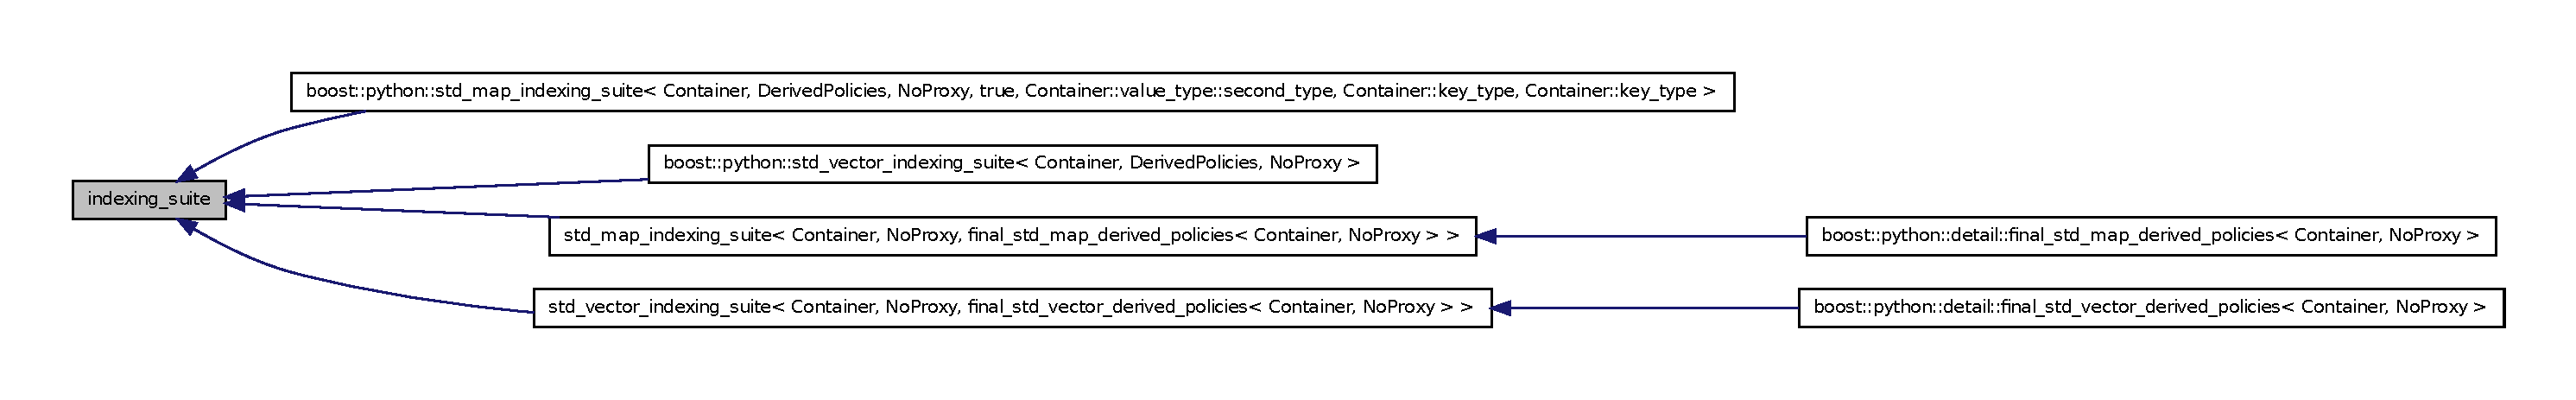
\includegraphics[width=350pt]{classindexing__suite__inherit__graph}
\end{center}
\end{figure}


\-The documentation for this class was generated from the following file\-:\begin{DoxyCompactItemize}
\item 
/home/vrabaud/workspace/recognition\-\_\-kitchen\-\_\-groovy/src/ecto/include/ecto/python/\hyperlink{std__vector__indexing__suite_8hpp}{std\-\_\-vector\-\_\-indexing\-\_\-suite.\-hpp}\end{DoxyCompactItemize}

\hypertarget{structboost_1_1python_1_1std__map__indexing__suite_1_1init__factory}{\section{boost\-:\-:python\-:\-:std\-\_\-map\-\_\-indexing\-\_\-suite$<$ Container, No\-Proxy, Derived\-Policies $>$\-:\-:init\-\_\-factory$<$ Py\-Class\-T $>$ Struct Template Reference}
\label{structboost_1_1python_1_1std__map__indexing__suite_1_1init__factory}\index{boost\-::python\-::std\-\_\-map\-\_\-indexing\-\_\-suite$<$ Container, No\-Proxy, Derived\-Policies $>$\-::init\-\_\-factory$<$ Py\-Class\-T $>$@{boost\-::python\-::std\-\_\-map\-\_\-indexing\-\_\-suite$<$ Container, No\-Proxy, Derived\-Policies $>$\-::init\-\_\-factory$<$ Py\-Class\-T $>$}}
}


{\ttfamily \#include $<$std\-\_\-map\-\_\-indexing\-\_\-suite.\-hpp$>$}

\subsection*{Public Types}
\begin{DoxyCompactItemize}
\item 
typedef Py\-Class\-T\-::metadata\-::holder \hyperlink{structboost_1_1python_1_1std__map__indexing__suite_1_1init__factory_a785b4c017210dd048b47eb6c04a5cdc6}{Holder}
\item 
typedef bp\-::objects\-::instance\\*
$<$ \hyperlink{structboost_1_1python_1_1std__map__indexing__suite_1_1init__factory_a785b4c017210dd048b47eb6c04a5cdc6}{Holder} $>$ \hyperlink{structboost_1_1python_1_1std__map__indexing__suite_1_1init__factory_aea2971d45c2f4de6ac83494b504d9a19}{instance\-\_\-t}
\end{DoxyCompactItemize}
\subsection*{Static Public Member Functions}
\begin{DoxyCompactItemize}
\item 
static void \hyperlink{structboost_1_1python_1_1std__map__indexing__suite_1_1init__factory_acd1c1789efbbb4f595abae51b1f0a2a0}{make\-\_\-holder} (Py\-Object $\ast$p)
\item 
static void \hyperlink{structboost_1_1python_1_1std__map__indexing__suite_1_1init__factory_aa1f0944f15cb284c240d25bfa6f0ccca}{from\-\_\-dict} (Py\-Object $\ast$p, bp\-::dict const \&dict)
\item 
static void \hyperlink{structboost_1_1python_1_1std__map__indexing__suite_1_1init__factory_ad0dbf8e2c1b8fa7dd7ecf87415e7d3fb}{from\-\_\-list} (Py\-Object $\ast$p, bp\-::list const \&list)
\end{DoxyCompactItemize}


\subsection{Member Typedef Documentation}
\hypertarget{structboost_1_1python_1_1std__map__indexing__suite_1_1init__factory_a785b4c017210dd048b47eb6c04a5cdc6}{\index{boost\-::python\-::std\-\_\-map\-\_\-indexing\-\_\-suite\-::init\-\_\-factory@{boost\-::python\-::std\-\_\-map\-\_\-indexing\-\_\-suite\-::init\-\_\-factory}!Holder@{Holder}}
\index{Holder@{Holder}!boost::python::std_map_indexing_suite::init_factory@{boost\-::python\-::std\-\_\-map\-\_\-indexing\-\_\-suite\-::init\-\_\-factory}}
\subsubsection[{Holder}]{\setlength{\rightskip}{0pt plus 5cm}template$<$class Container, bool No\-Proxy, class Derived\-Policies$>$ template$<$typename Py\-Class\-T $>$ typedef Py\-Class\-T\-::metadata\-::holder {\bf boost\-::python\-::std\-\_\-map\-\_\-indexing\-\_\-suite}$<$ Container, No\-Proxy, Derived\-Policies $>$\-::{\bf init\-\_\-factory}$<$ Py\-Class\-T $>$\-::{\bf Holder}}}\label{structboost_1_1python_1_1std__map__indexing__suite_1_1init__factory_a785b4c017210dd048b47eb6c04a5cdc6}
\hypertarget{structboost_1_1python_1_1std__map__indexing__suite_1_1init__factory_aea2971d45c2f4de6ac83494b504d9a19}{\index{boost\-::python\-::std\-\_\-map\-\_\-indexing\-\_\-suite\-::init\-\_\-factory@{boost\-::python\-::std\-\_\-map\-\_\-indexing\-\_\-suite\-::init\-\_\-factory}!instance\-\_\-t@{instance\-\_\-t}}
\index{instance\-\_\-t@{instance\-\_\-t}!boost::python::std_map_indexing_suite::init_factory@{boost\-::python\-::std\-\_\-map\-\_\-indexing\-\_\-suite\-::init\-\_\-factory}}
\subsubsection[{instance\-\_\-t}]{\setlength{\rightskip}{0pt plus 5cm}template$<$class Container, bool No\-Proxy, class Derived\-Policies$>$ template$<$typename Py\-Class\-T $>$ typedef bp\-::objects\-::instance$<${\bf Holder}$>$ {\bf boost\-::python\-::std\-\_\-map\-\_\-indexing\-\_\-suite}$<$ Container, No\-Proxy, Derived\-Policies $>$\-::{\bf init\-\_\-factory}$<$ Py\-Class\-T $>$\-::{\bf instance\-\_\-t}}}\label{structboost_1_1python_1_1std__map__indexing__suite_1_1init__factory_aea2971d45c2f4de6ac83494b504d9a19}


\subsection{Member Function Documentation}
\hypertarget{structboost_1_1python_1_1std__map__indexing__suite_1_1init__factory_aa1f0944f15cb284c240d25bfa6f0ccca}{\index{boost\-::python\-::std\-\_\-map\-\_\-indexing\-\_\-suite\-::init\-\_\-factory@{boost\-::python\-::std\-\_\-map\-\_\-indexing\-\_\-suite\-::init\-\_\-factory}!from\-\_\-dict@{from\-\_\-dict}}
\index{from\-\_\-dict@{from\-\_\-dict}!boost::python::std_map_indexing_suite::init_factory@{boost\-::python\-::std\-\_\-map\-\_\-indexing\-\_\-suite\-::init\-\_\-factory}}
\subsubsection[{from\-\_\-dict}]{\setlength{\rightskip}{0pt plus 5cm}template$<$class Container, bool No\-Proxy, class Derived\-Policies$>$ template$<$typename Py\-Class\-T $>$ static void {\bf boost\-::python\-::std\-\_\-map\-\_\-indexing\-\_\-suite}$<$ Container, No\-Proxy, Derived\-Policies $>$\-::{\bf init\-\_\-factory}$<$ Py\-Class\-T $>$\-::from\-\_\-dict (
\begin{DoxyParamCaption}
\item[{Py\-Object $\ast$}]{p, }
\item[{bp\-::dict const \&}]{dict}
\end{DoxyParamCaption}
)\hspace{0.3cm}{\ttfamily [inline]}, {\ttfamily [static]}}}\label{structboost_1_1python_1_1std__map__indexing__suite_1_1init__factory_aa1f0944f15cb284c240d25bfa6f0ccca}
\hypertarget{structboost_1_1python_1_1std__map__indexing__suite_1_1init__factory_ad0dbf8e2c1b8fa7dd7ecf87415e7d3fb}{\index{boost\-::python\-::std\-\_\-map\-\_\-indexing\-\_\-suite\-::init\-\_\-factory@{boost\-::python\-::std\-\_\-map\-\_\-indexing\-\_\-suite\-::init\-\_\-factory}!from\-\_\-list@{from\-\_\-list}}
\index{from\-\_\-list@{from\-\_\-list}!boost::python::std_map_indexing_suite::init_factory@{boost\-::python\-::std\-\_\-map\-\_\-indexing\-\_\-suite\-::init\-\_\-factory}}
\subsubsection[{from\-\_\-list}]{\setlength{\rightskip}{0pt plus 5cm}template$<$class Container, bool No\-Proxy, class Derived\-Policies$>$ template$<$typename Py\-Class\-T $>$ static void {\bf boost\-::python\-::std\-\_\-map\-\_\-indexing\-\_\-suite}$<$ Container, No\-Proxy, Derived\-Policies $>$\-::{\bf init\-\_\-factory}$<$ Py\-Class\-T $>$\-::from\-\_\-list (
\begin{DoxyParamCaption}
\item[{Py\-Object $\ast$}]{p, }
\item[{bp\-::list const \&}]{list}
\end{DoxyParamCaption}
)\hspace{0.3cm}{\ttfamily [inline]}, {\ttfamily [static]}}}\label{structboost_1_1python_1_1std__map__indexing__suite_1_1init__factory_ad0dbf8e2c1b8fa7dd7ecf87415e7d3fb}
\hypertarget{structboost_1_1python_1_1std__map__indexing__suite_1_1init__factory_acd1c1789efbbb4f595abae51b1f0a2a0}{\index{boost\-::python\-::std\-\_\-map\-\_\-indexing\-\_\-suite\-::init\-\_\-factory@{boost\-::python\-::std\-\_\-map\-\_\-indexing\-\_\-suite\-::init\-\_\-factory}!make\-\_\-holder@{make\-\_\-holder}}
\index{make\-\_\-holder@{make\-\_\-holder}!boost::python::std_map_indexing_suite::init_factory@{boost\-::python\-::std\-\_\-map\-\_\-indexing\-\_\-suite\-::init\-\_\-factory}}
\subsubsection[{make\-\_\-holder}]{\setlength{\rightskip}{0pt plus 5cm}template$<$class Container, bool No\-Proxy, class Derived\-Policies$>$ template$<$typename Py\-Class\-T $>$ static void {\bf boost\-::python\-::std\-\_\-map\-\_\-indexing\-\_\-suite}$<$ Container, No\-Proxy, Derived\-Policies $>$\-::{\bf init\-\_\-factory}$<$ Py\-Class\-T $>$\-::make\-\_\-holder (
\begin{DoxyParamCaption}
\item[{Py\-Object $\ast$}]{p}
\end{DoxyParamCaption}
)\hspace{0.3cm}{\ttfamily [inline]}, {\ttfamily [static]}}}\label{structboost_1_1python_1_1std__map__indexing__suite_1_1init__factory_acd1c1789efbbb4f595abae51b1f0a2a0}


The documentation for this struct was generated from the following file\-:\begin{DoxyCompactItemize}
\item 
/home/vrabaud/workspace/recognition\-\_\-kitchen/src/ecto/include/ecto/python/\hyperlink{std__map__indexing__suite_8hpp}{std\-\_\-map\-\_\-indexing\-\_\-suite.\-hpp}\end{DoxyCompactItemize}

\hypertarget{structecto_1_1cell___1_1int__}{}\section{ecto\+:\+:cell\+\_\+$<$ Impl $>$\+:\+:int\+\_\+$<$ I $>$ Struct Template Reference}
\label{structecto_1_1cell___1_1int__}\index{ecto\+::cell\+\_\+$<$ Impl $>$\+::int\+\_\+$<$ I $>$@{ecto\+::cell\+\_\+$<$ Impl $>$\+::int\+\_\+$<$ I $>$}}


{\ttfamily \#include $<$cell.\+hpp$>$}



The documentation for this struct was generated from the following file\+:\begin{DoxyCompactItemize}
\item 
/home/vrabaud/workspace/recognition\+\_\+kitchen/src/ecto/include/ecto/\hyperlink{cell_8hpp}{cell.\+hpp}\end{DoxyCompactItemize}

\hypertarget{structecto_1_1detail_1_1is__threadsafe}{\section{ecto\-:\-:detail\-:\-:is\-\_\-threadsafe$<$ \-T $>$ \-Struct \-Template \-Reference}
\label{structecto_1_1detail_1_1is__threadsafe}\index{ecto\-::detail\-::is\-\_\-threadsafe$<$ T $>$@{ecto\-::detail\-::is\-\_\-threadsafe$<$ T $>$}}
}


{\ttfamily \#include $<$traits.\-hpp$>$}

\subsubsection*{template$<$typename T$>$ struct ecto\-::detail\-::is\-\_\-threadsafe$<$ T $>$}



\-The documentation for this struct was generated from the following file\-:\begin{DoxyCompactItemize}
\item 
/home/vrabaud/workspace/recognition\-\_\-kitchen\-\_\-groovy/src/ecto/include/ecto/\hyperlink{traits_8hpp}{traits.\-hpp}\end{DoxyCompactItemize}

\hypertarget{classecto_1_1py_1_1streambuf_1_1istream}{\section{ecto\-:\-:py\-:\-:streambuf\-:\-:istream Class Reference}
\label{classecto_1_1py_1_1streambuf_1_1istream}\index{ecto\-::py\-::streambuf\-::istream@{ecto\-::py\-::streambuf\-::istream}}
}


{\ttfamily \#include $<$streambuf.\-hpp$>$}



Inheritance diagram for ecto\-:\-:py\-:\-:streambuf\-:\-:istream\-:\nopagebreak
\begin{figure}[H]
\begin{center}
\leavevmode
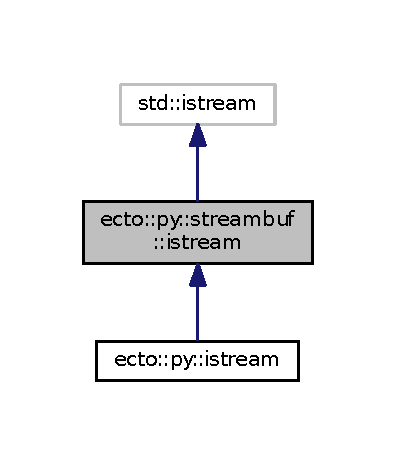
\includegraphics[width=190pt]{classecto_1_1py_1_1streambuf_1_1istream__inherit__graph}
\end{center}
\end{figure}


Collaboration diagram for ecto\-:\-:py\-:\-:streambuf\-:\-:istream\-:\nopagebreak
\begin{figure}[H]
\begin{center}
\leavevmode
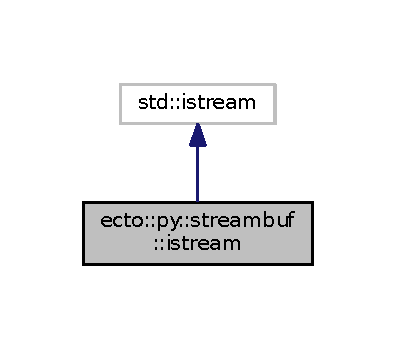
\includegraphics[width=190pt]{classecto_1_1py_1_1streambuf_1_1istream__coll__graph}
\end{center}
\end{figure}
\subsection*{Public Member Functions}
\begin{DoxyCompactItemize}
\item 
\hyperlink{classecto_1_1py_1_1streambuf_1_1istream_aff2d95cb5e4b1113f873b7a7e1cead29}{istream} (\hyperlink{classecto_1_1py_1_1streambuf}{streambuf} \&buf)
\item 
\hyperlink{classecto_1_1py_1_1streambuf_1_1istream_ab53f3c2893d995a22ef2374ce9a00004}{$\sim$istream} ()
\end{DoxyCompactItemize}


\subsection{Constructor \& Destructor Documentation}
\hypertarget{classecto_1_1py_1_1streambuf_1_1istream_aff2d95cb5e4b1113f873b7a7e1cead29}{\index{ecto\-::py\-::streambuf\-::istream@{ecto\-::py\-::streambuf\-::istream}!istream@{istream}}
\index{istream@{istream}!ecto::py::streambuf::istream@{ecto\-::py\-::streambuf\-::istream}}
\subsubsection[{istream}]{\setlength{\rightskip}{0pt plus 5cm}ecto\-::py\-::streambuf\-::istream\-::istream (
\begin{DoxyParamCaption}
\item[{{\bf streambuf} \&}]{buf}
\end{DoxyParamCaption}
)\hspace{0.3cm}{\ttfamily [inline]}}}\label{classecto_1_1py_1_1streambuf_1_1istream_aff2d95cb5e4b1113f873b7a7e1cead29}
\hypertarget{classecto_1_1py_1_1streambuf_1_1istream_ab53f3c2893d995a22ef2374ce9a00004}{\index{ecto\-::py\-::streambuf\-::istream@{ecto\-::py\-::streambuf\-::istream}!$\sim$istream@{$\sim$istream}}
\index{$\sim$istream@{$\sim$istream}!ecto::py::streambuf::istream@{ecto\-::py\-::streambuf\-::istream}}
\subsubsection[{$\sim$istream}]{\setlength{\rightskip}{0pt plus 5cm}ecto\-::py\-::streambuf\-::istream\-::$\sim$istream (
\begin{DoxyParamCaption}
{}
\end{DoxyParamCaption}
)\hspace{0.3cm}{\ttfamily [inline]}}}\label{classecto_1_1py_1_1streambuf_1_1istream_ab53f3c2893d995a22ef2374ce9a00004}


The documentation for this class was generated from the following file\-:\begin{DoxyCompactItemize}
\item 
/home/vrabaud/workspace/recognition\-\_\-kitchen/src/ecto/include/ecto/python/\hyperlink{streambuf_8hpp}{streambuf.\-hpp}\end{DoxyCompactItemize}

\hypertarget{structecto_1_1py_1_1istream}{\section{ecto\-:\-:py\-:\-:istream Struct Reference}
\label{structecto_1_1py_1_1istream}\index{ecto\-::py\-::istream@{ecto\-::py\-::istream}}
}


{\ttfamily \#include $<$streambuf.\-hpp$>$}



Inheritance diagram for ecto\-:\-:py\-:\-:istream\-:\nopagebreak
\begin{figure}[H]
\begin{center}
\leavevmode
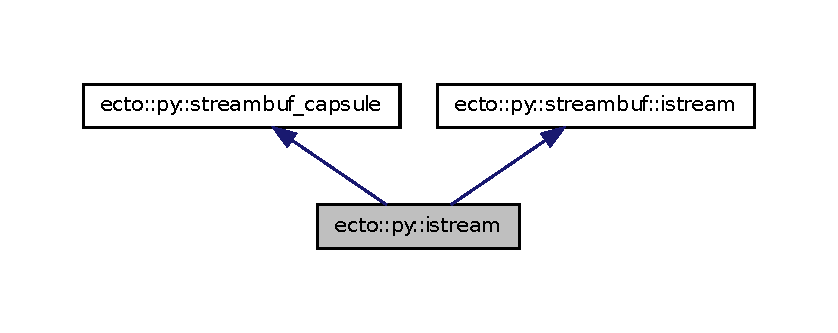
\includegraphics[width=318pt]{structecto_1_1py_1_1istream__inherit__graph}
\end{center}
\end{figure}


Collaboration diagram for ecto\-:\-:py\-:\-:istream\-:\nopagebreak
\begin{figure}[H]
\begin{center}
\leavevmode
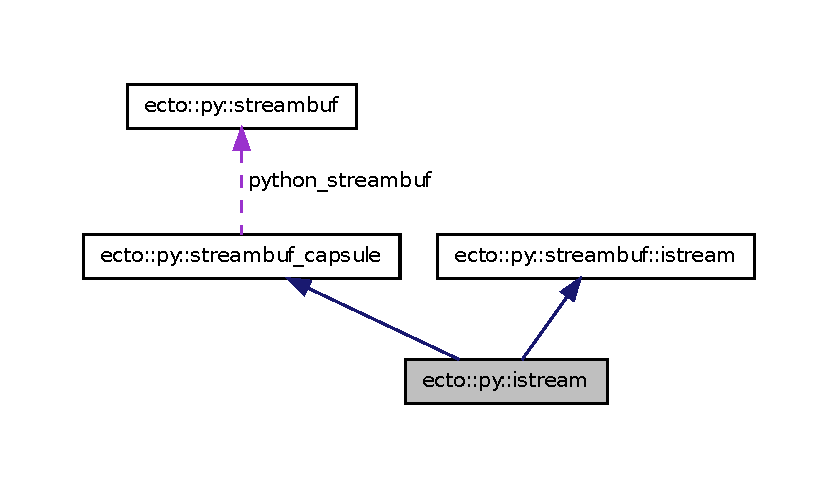
\includegraphics[width=321pt]{structecto_1_1py_1_1istream__coll__graph}
\end{center}
\end{figure}
\subsection*{Public Member Functions}
\begin{DoxyCompactItemize}
\item 
\hyperlink{structecto_1_1py_1_1istream_a1261100ee2202be4989166b6a16fc1b0}{istream} (bp\-::object \&python\-\_\-file\-\_\-obj, std\-::size\-\_\-t buffer\-\_\-size=0)
\end{DoxyCompactItemize}
\subsection*{Additional Inherited Members}


\subsection{Constructor \& Destructor Documentation}
\hypertarget{structecto_1_1py_1_1istream_a1261100ee2202be4989166b6a16fc1b0}{\index{ecto\-::py\-::istream@{ecto\-::py\-::istream}!istream@{istream}}
\index{istream@{istream}!ecto::py::istream@{ecto\-::py\-::istream}}
\subsubsection[{istream}]{\setlength{\rightskip}{0pt plus 5cm}ecto\-::py\-::istream\-::istream (
\begin{DoxyParamCaption}
\item[{bp\-::object \&}]{python\-\_\-file\-\_\-obj, }
\item[{std\-::size\-\_\-t}]{buffer\-\_\-size = {\ttfamily 0}}
\end{DoxyParamCaption}
)\hspace{0.3cm}{\ttfamily [inline]}}}\label{structecto_1_1py_1_1istream_a1261100ee2202be4989166b6a16fc1b0}


The documentation for this struct was generated from the following file\-:\begin{DoxyCompactItemize}
\item 
/home/vrabaud/workspace/recognition\-\_\-kitchen/src/ecto/include/ecto/python/\hyperlink{streambuf_8hpp}{streambuf.\-hpp}\end{DoxyCompactItemize}

\hypertarget{structboost_1_1python_1_1std__map__indexing__suite_1_1iteritems}{\section{boost\-:\-:python\-:\-:std\-\_\-map\-\_\-indexing\-\_\-suite$<$ \-Container, \-No\-Proxy, \-Derived\-Policies $>$\-:\-:iteritems \-Struct \-Reference}
\label{structboost_1_1python_1_1std__map__indexing__suite_1_1iteritems}\index{boost\-::python\-::std\-\_\-map\-\_\-indexing\-\_\-suite$<$ Container, No\-Proxy, Derived\-Policies $>$\-::iteritems@{boost\-::python\-::std\-\_\-map\-\_\-indexing\-\_\-suite$<$ Container, No\-Proxy, Derived\-Policies $>$\-::iteritems}}
}


{\ttfamily \#include $<$std\-\_\-map\-\_\-indexing\-\_\-suite.\-hpp$>$}

\subsection*{\-Public \-Types}
\begin{DoxyCompactItemize}
\item 
typedef tuple \hyperlink{structboost_1_1python_1_1std__map__indexing__suite_1_1iteritems_a97f1c788acd4c665fba8ae1fcc946a45}{result\-\_\-type}
\end{DoxyCompactItemize}
\subsection*{\-Public \-Member \-Functions}
\begin{DoxyCompactItemize}
\item 
\hyperlink{structboost_1_1python_1_1std__map__indexing__suite_1_1iteritems_a97f1c788acd4c665fba8ae1fcc946a45}{result\-\_\-type} \hyperlink{structboost_1_1python_1_1std__map__indexing__suite_1_1iteritems_a4adb01be48bc47d6c1636957267fdca2}{operator()} (\hyperlink{classboost_1_1python_1_1std__map__indexing__suite_aff9ed68cf30e805a04a313d92c62ab38}{value\-\_\-type} const \&x) const 
\end{DoxyCompactItemize}
\subsubsection*{template$<$class \-Container, bool \-No\-Proxy = false, class \-Derived\-Policies = detail\-::final\-\_\-std\-\_\-map\-\_\-derived\-\_\-policies$<$\-Container, No\-Proxy$>$$>$ struct boost\-::python\-::std\-\_\-map\-\_\-indexing\-\_\-suite$<$ Container, No\-Proxy, Derived\-Policies $>$\-::iteritems}



\subsection{\-Member \-Typedef \-Documentation}
\hypertarget{structboost_1_1python_1_1std__map__indexing__suite_1_1iteritems_a97f1c788acd4c665fba8ae1fcc946a45}{\index{boost\-::python\-::std\-\_\-map\-\_\-indexing\-\_\-suite\-::iteritems@{boost\-::python\-::std\-\_\-map\-\_\-indexing\-\_\-suite\-::iteritems}!result\-\_\-type@{result\-\_\-type}}
\index{result\-\_\-type@{result\-\_\-type}!boost::python::std_map_indexing_suite::iteritems@{boost\-::python\-::std\-\_\-map\-\_\-indexing\-\_\-suite\-::iteritems}}
\subsubsection[{result\-\_\-type}]{\setlength{\rightskip}{0pt plus 5cm}template$<$class \-Container, bool \-No\-Proxy = false, class \-Derived\-Policies = detail\-::final\-\_\-std\-\_\-map\-\_\-derived\-\_\-policies$<$\-Container, No\-Proxy$>$$>$ typedef tuple {\bf boost\-::python\-::std\-\_\-map\-\_\-indexing\-\_\-suite}$<$ \-Container, \-No\-Proxy, \-Derived\-Policies $>$\-::{\bf iteritems\-::result\-\_\-type}}}\label{structboost_1_1python_1_1std__map__indexing__suite_1_1iteritems_a97f1c788acd4c665fba8ae1fcc946a45}


\subsection{\-Member \-Function \-Documentation}
\hypertarget{structboost_1_1python_1_1std__map__indexing__suite_1_1iteritems_a4adb01be48bc47d6c1636957267fdca2}{\index{boost\-::python\-::std\-\_\-map\-\_\-indexing\-\_\-suite\-::iteritems@{boost\-::python\-::std\-\_\-map\-\_\-indexing\-\_\-suite\-::iteritems}!operator()@{operator()}}
\index{operator()@{operator()}!boost::python::std_map_indexing_suite::iteritems@{boost\-::python\-::std\-\_\-map\-\_\-indexing\-\_\-suite\-::iteritems}}
\subsubsection[{operator()}]{\setlength{\rightskip}{0pt plus 5cm}template$<$class \-Container, bool \-No\-Proxy = false, class \-Derived\-Policies = detail\-::final\-\_\-std\-\_\-map\-\_\-derived\-\_\-policies$<$\-Container, No\-Proxy$>$$>$ {\bf result\-\_\-type} {\bf boost\-::python\-::std\-\_\-map\-\_\-indexing\-\_\-suite}$<$ \-Container, \-No\-Proxy, \-Derived\-Policies $>$\-::iteritems\-::operator() (
\begin{DoxyParamCaption}
\item[{{\bf value\-\_\-type} const \&}]{x}
\end{DoxyParamCaption}
) const\hspace{0.3cm}{\ttfamily  \mbox{[}inline\mbox{]}}}}\label{structboost_1_1python_1_1std__map__indexing__suite_1_1iteritems_a4adb01be48bc47d6c1636957267fdca2}


\-The documentation for this struct was generated from the following file\-:\begin{DoxyCompactItemize}
\item 
/home/vrabaud/workspace/recognition\-\_\-kitchen\-\_\-groovy/src/ecto/include/ecto/python/\hyperlink{std__map__indexing__suite_8hpp}{std\-\_\-map\-\_\-indexing\-\_\-suite.\-hpp}\end{DoxyCompactItemize}

\hypertarget{structboost_1_1python_1_1std__map__indexing__suite_1_1iterkeys}{}\section{boost\+:\+:python\+:\+:std\+\_\+map\+\_\+indexing\+\_\+suite$<$ Container, No\+Proxy, Derived\+Policies $>$\+:\+:iterkeys Struct Reference}
\label{structboost_1_1python_1_1std__map__indexing__suite_1_1iterkeys}\index{boost\+::python\+::std\+\_\+map\+\_\+indexing\+\_\+suite$<$ Container, No\+Proxy, Derived\+Policies $>$\+::iterkeys@{boost\+::python\+::std\+\_\+map\+\_\+indexing\+\_\+suite$<$ Container, No\+Proxy, Derived\+Policies $>$\+::iterkeys}}


{\ttfamily \#include $<$std\+\_\+map\+\_\+indexing\+\_\+suite.\+hpp$>$}

\subsection*{Public Types}
\begin{DoxyCompactItemize}
\item 
typedef \hyperlink{classboost_1_1python_1_1std__map__indexing__suite_a4e2daeb60a58d6ce9964e0ea27680009}{key\+\_\+type} \hyperlink{structboost_1_1python_1_1std__map__indexing__suite_1_1iterkeys_a7c12b5aeae081d2ecf524e29e5a5c343}{result\+\_\+type}
\end{DoxyCompactItemize}
\subsection*{Public Member Functions}
\begin{DoxyCompactItemize}
\item 
\hyperlink{structboost_1_1python_1_1std__map__indexing__suite_1_1iterkeys_a7c12b5aeae081d2ecf524e29e5a5c343}{result\+\_\+type} \hyperlink{structboost_1_1python_1_1std__map__indexing__suite_1_1iterkeys_a0e3b853fc4bbcc4777e5c663cc8bdd60}{operator()} (\hyperlink{classboost_1_1python_1_1std__map__indexing__suite_aff9ed68cf30e805a04a313d92c62ab38}{value\+\_\+type} const \&x) const 
\end{DoxyCompactItemize}


\subsection{Member Typedef Documentation}
\hypertarget{structboost_1_1python_1_1std__map__indexing__suite_1_1iterkeys_a7c12b5aeae081d2ecf524e29e5a5c343}{}\index{boost\+::python\+::std\+\_\+map\+\_\+indexing\+\_\+suite\+::iterkeys@{boost\+::python\+::std\+\_\+map\+\_\+indexing\+\_\+suite\+::iterkeys}!result\+\_\+type@{result\+\_\+type}}
\index{result\+\_\+type@{result\+\_\+type}!boost\+::python\+::std\+\_\+map\+\_\+indexing\+\_\+suite\+::iterkeys@{boost\+::python\+::std\+\_\+map\+\_\+indexing\+\_\+suite\+::iterkeys}}
\subsubsection[{result\+\_\+type}]{\setlength{\rightskip}{0pt plus 5cm}template$<$class Container, bool No\+Proxy = false, class Derived\+Policies = detail\+::final\+\_\+std\+\_\+map\+\_\+derived\+\_\+policies$<$\+Container, No\+Proxy$>$$>$ typedef {\bf key\+\_\+type} {\bf boost\+::python\+::std\+\_\+map\+\_\+indexing\+\_\+suite}$<$ Container, No\+Proxy, Derived\+Policies $>$\+::{\bf iterkeys\+::result\+\_\+type}}\label{structboost_1_1python_1_1std__map__indexing__suite_1_1iterkeys_a7c12b5aeae081d2ecf524e29e5a5c343}


\subsection{Member Function Documentation}
\hypertarget{structboost_1_1python_1_1std__map__indexing__suite_1_1iterkeys_a0e3b853fc4bbcc4777e5c663cc8bdd60}{}\index{boost\+::python\+::std\+\_\+map\+\_\+indexing\+\_\+suite\+::iterkeys@{boost\+::python\+::std\+\_\+map\+\_\+indexing\+\_\+suite\+::iterkeys}!operator()@{operator()}}
\index{operator()@{operator()}!boost\+::python\+::std\+\_\+map\+\_\+indexing\+\_\+suite\+::iterkeys@{boost\+::python\+::std\+\_\+map\+\_\+indexing\+\_\+suite\+::iterkeys}}
\subsubsection[{operator()}]{\setlength{\rightskip}{0pt plus 5cm}template$<$class Container, bool No\+Proxy = false, class Derived\+Policies = detail\+::final\+\_\+std\+\_\+map\+\_\+derived\+\_\+policies$<$\+Container, No\+Proxy$>$$>$ {\bf result\+\_\+type} {\bf boost\+::python\+::std\+\_\+map\+\_\+indexing\+\_\+suite}$<$ Container, No\+Proxy, Derived\+Policies $>$\+::iterkeys\+::operator() (
\begin{DoxyParamCaption}
\item[{{\bf value\+\_\+type} const \&}]{x}
\end{DoxyParamCaption}
) const\hspace{0.3cm}{\ttfamily [inline]}}\label{structboost_1_1python_1_1std__map__indexing__suite_1_1iterkeys_a0e3b853fc4bbcc4777e5c663cc8bdd60}


The documentation for this struct was generated from the following file\+:\begin{DoxyCompactItemize}
\item 
/home/vrabaud/workspace/recognition\+\_\+kitchen/src/ecto/include/ecto/python/\hyperlink{std__map__indexing__suite_8hpp}{std\+\_\+map\+\_\+indexing\+\_\+suite.\+hpp}\end{DoxyCompactItemize}

\hypertarget{structboost_1_1python_1_1std__map__indexing__suite_1_1itervalues}{}\section{boost\+:\+:python\+:\+:std\+\_\+map\+\_\+indexing\+\_\+suite$<$ Container, No\+Proxy, Derived\+Policies $>$\+:\+:itervalues Struct Reference}
\label{structboost_1_1python_1_1std__map__indexing__suite_1_1itervalues}\index{boost\+::python\+::std\+\_\+map\+\_\+indexing\+\_\+suite$<$ Container, No\+Proxy, Derived\+Policies $>$\+::itervalues@{boost\+::python\+::std\+\_\+map\+\_\+indexing\+\_\+suite$<$ Container, No\+Proxy, Derived\+Policies $>$\+::itervalues}}


{\ttfamily \#include $<$std\+\_\+map\+\_\+indexing\+\_\+suite.\+hpp$>$}

\subsection*{Public Types}
\begin{DoxyCompactItemize}
\item 
typedef \hyperlink{classboost_1_1python_1_1std__map__indexing__suite_a3e9a6a8b8ba34759cf0ba99fe5966041}{data\+\_\+type} \hyperlink{structboost_1_1python_1_1std__map__indexing__suite_1_1itervalues_a7d2f8df7d18009f2bad1363db4f718f3}{result\+\_\+type}
\end{DoxyCompactItemize}
\subsection*{Public Member Functions}
\begin{DoxyCompactItemize}
\item 
\hyperlink{structboost_1_1python_1_1std__map__indexing__suite_1_1itervalues_a7d2f8df7d18009f2bad1363db4f718f3}{result\+\_\+type} \hyperlink{structboost_1_1python_1_1std__map__indexing__suite_1_1itervalues_a36486ce19f8e08900aabe582d0502dc8}{operator()} (\hyperlink{classboost_1_1python_1_1std__map__indexing__suite_aff9ed68cf30e805a04a313d92c62ab38}{value\+\_\+type} const \&x) const 
\end{DoxyCompactItemize}


\subsection{Member Typedef Documentation}
\index{boost\+::python\+::std\+\_\+map\+\_\+indexing\+\_\+suite\+::itervalues@{boost\+::python\+::std\+\_\+map\+\_\+indexing\+\_\+suite\+::itervalues}!result\+\_\+type@{result\+\_\+type}}
\index{result\+\_\+type@{result\+\_\+type}!boost\+::python\+::std\+\_\+map\+\_\+indexing\+\_\+suite\+::itervalues@{boost\+::python\+::std\+\_\+map\+\_\+indexing\+\_\+suite\+::itervalues}}
\subsubsection[{\texorpdfstring{result\+\_\+type}{result_type}}]{\setlength{\rightskip}{0pt plus 5cm}template$<$class Container, bool No\+Proxy = false, class Derived\+Policies = detail\+::final\+\_\+std\+\_\+map\+\_\+derived\+\_\+policies$<$\+Container, No\+Proxy$>$$>$ typedef {\bf data\+\_\+type} {\bf boost\+::python\+::std\+\_\+map\+\_\+indexing\+\_\+suite}$<$ Container, No\+Proxy, Derived\+Policies $>$\+::{\bf itervalues\+::result\+\_\+type}}\hypertarget{structboost_1_1python_1_1std__map__indexing__suite_1_1itervalues_a7d2f8df7d18009f2bad1363db4f718f3}{}\label{structboost_1_1python_1_1std__map__indexing__suite_1_1itervalues_a7d2f8df7d18009f2bad1363db4f718f3}


\subsection{Member Function Documentation}
\index{boost\+::python\+::std\+\_\+map\+\_\+indexing\+\_\+suite\+::itervalues@{boost\+::python\+::std\+\_\+map\+\_\+indexing\+\_\+suite\+::itervalues}!operator()@{operator()}}
\index{operator()@{operator()}!boost\+::python\+::std\+\_\+map\+\_\+indexing\+\_\+suite\+::itervalues@{boost\+::python\+::std\+\_\+map\+\_\+indexing\+\_\+suite\+::itervalues}}
\subsubsection[{\texorpdfstring{operator()(value\+\_\+type const \&x) const }{operator()(value_type const &x) const }}]{\setlength{\rightskip}{0pt plus 5cm}template$<$class Container, bool No\+Proxy = false, class Derived\+Policies = detail\+::final\+\_\+std\+\_\+map\+\_\+derived\+\_\+policies$<$\+Container, No\+Proxy$>$$>$ {\bf result\+\_\+type} {\bf boost\+::python\+::std\+\_\+map\+\_\+indexing\+\_\+suite}$<$ Container, No\+Proxy, Derived\+Policies $>$\+::itervalues\+::operator() (
\begin{DoxyParamCaption}
\item[{{\bf value\+\_\+type} const \&}]{x}
\end{DoxyParamCaption}
) const\hspace{0.3cm}{\ttfamily [inline]}}\hypertarget{structboost_1_1python_1_1std__map__indexing__suite_1_1itervalues_a36486ce19f8e08900aabe582d0502dc8}{}\label{structboost_1_1python_1_1std__map__indexing__suite_1_1itervalues_a36486ce19f8e08900aabe582d0502dc8}


The documentation for this struct was generated from the following file\+:\begin{DoxyCompactItemize}
\item 
/home/vrabaud/workspace/recognition\+\_\+kitchen/src/ecto/include/ecto/python/\hyperlink{std__map__indexing__suite_8hpp}{std\+\_\+map\+\_\+indexing\+\_\+suite.\+hpp}\end{DoxyCompactItemize}

\hypertarget{structboost_1_1python_1_1std__map__indexing__suite_1_1make__transform__impl}{}\section{boost\+:\+:python\+:\+:std\+\_\+map\+\_\+indexing\+\_\+suite$<$ Container, No\+Proxy, Derived\+Policies $>$\+:\+:make\+\_\+transform\+\_\+impl$<$ Transform $>$ Struct Template Reference}
\label{structboost_1_1python_1_1std__map__indexing__suite_1_1make__transform__impl}\index{boost\+::python\+::std\+\_\+map\+\_\+indexing\+\_\+suite$<$ Container, No\+Proxy, Derived\+Policies $>$\+::make\+\_\+transform\+\_\+impl$<$ Transform $>$@{boost\+::python\+::std\+\_\+map\+\_\+indexing\+\_\+suite$<$ Container, No\+Proxy, Derived\+Policies $>$\+::make\+\_\+transform\+\_\+impl$<$ Transform $>$}}


{\ttfamily \#include $<$std\+\_\+map\+\_\+indexing\+\_\+suite.\+hpp$>$}

\subsection*{Public Types}
\begin{DoxyCompactItemize}
\item 
typedef boost\+::transform\+\_\+iterator$<$ Transform, \hyperlink{classboost_1_1python_1_1std__map__indexing__suite_aae0c4473455223a4e048cc207ca7b3ea}{const\+\_\+iterator} $>$ \hyperlink{structboost_1_1python_1_1std__map__indexing__suite_1_1make__transform__impl_a64d7b60f0e792533c1cc89b84f341b0d}{iterator}
\end{DoxyCompactItemize}
\subsection*{Static Public Member Functions}
\begin{DoxyCompactItemize}
\item 
static \hyperlink{structboost_1_1python_1_1std__map__indexing__suite_1_1make__transform__impl_a64d7b60f0e792533c1cc89b84f341b0d}{iterator} \hyperlink{structboost_1_1python_1_1std__map__indexing__suite_1_1make__transform__impl_ab74967f0d94cdc5adcae986110974656}{begin} (const Container \&m)
\item 
static \hyperlink{structboost_1_1python_1_1std__map__indexing__suite_1_1make__transform__impl_a64d7b60f0e792533c1cc89b84f341b0d}{iterator} \hyperlink{structboost_1_1python_1_1std__map__indexing__suite_1_1make__transform__impl_ac8c3535052a0a3320e73ab5b49eb6b82}{end} (const Container \&m)
\item 
static bp\+::object \hyperlink{structboost_1_1python_1_1std__map__indexing__suite_1_1make__transform__impl_a9dbcd293bf92f94f2eaeaed8edb64ee2}{range} ()
\end{DoxyCompactItemize}


\subsection{Member Typedef Documentation}
\hypertarget{structboost_1_1python_1_1std__map__indexing__suite_1_1make__transform__impl_a64d7b60f0e792533c1cc89b84f341b0d}{}\index{boost\+::python\+::std\+\_\+map\+\_\+indexing\+\_\+suite\+::make\+\_\+transform\+\_\+impl@{boost\+::python\+::std\+\_\+map\+\_\+indexing\+\_\+suite\+::make\+\_\+transform\+\_\+impl}!iterator@{iterator}}
\index{iterator@{iterator}!boost\+::python\+::std\+\_\+map\+\_\+indexing\+\_\+suite\+::make\+\_\+transform\+\_\+impl@{boost\+::python\+::std\+\_\+map\+\_\+indexing\+\_\+suite\+::make\+\_\+transform\+\_\+impl}}
\subsubsection[{iterator}]{\setlength{\rightskip}{0pt plus 5cm}template$<$class Container, bool No\+Proxy = false, class Derived\+Policies = detail\+::final\+\_\+std\+\_\+map\+\_\+derived\+\_\+policies$<$\+Container, No\+Proxy$>$$>$ template$<$typename Transform $>$ typedef boost\+::transform\+\_\+iterator$<$Transform, {\bf const\+\_\+iterator}$>$ {\bf boost\+::python\+::std\+\_\+map\+\_\+indexing\+\_\+suite}$<$ Container, No\+Proxy, Derived\+Policies $>$\+::{\bf make\+\_\+transform\+\_\+impl}$<$ Transform $>$\+::{\bf iterator}}\label{structboost_1_1python_1_1std__map__indexing__suite_1_1make__transform__impl_a64d7b60f0e792533c1cc89b84f341b0d}


\subsection{Member Function Documentation}
\hypertarget{structboost_1_1python_1_1std__map__indexing__suite_1_1make__transform__impl_ab74967f0d94cdc5adcae986110974656}{}\index{boost\+::python\+::std\+\_\+map\+\_\+indexing\+\_\+suite\+::make\+\_\+transform\+\_\+impl@{boost\+::python\+::std\+\_\+map\+\_\+indexing\+\_\+suite\+::make\+\_\+transform\+\_\+impl}!begin@{begin}}
\index{begin@{begin}!boost\+::python\+::std\+\_\+map\+\_\+indexing\+\_\+suite\+::make\+\_\+transform\+\_\+impl@{boost\+::python\+::std\+\_\+map\+\_\+indexing\+\_\+suite\+::make\+\_\+transform\+\_\+impl}}
\subsubsection[{begin}]{\setlength{\rightskip}{0pt plus 5cm}template$<$class Container, bool No\+Proxy = false, class Derived\+Policies = detail\+::final\+\_\+std\+\_\+map\+\_\+derived\+\_\+policies$<$\+Container, No\+Proxy$>$$>$ template$<$typename Transform $>$ static {\bf iterator} {\bf boost\+::python\+::std\+\_\+map\+\_\+indexing\+\_\+suite}$<$ Container, No\+Proxy, Derived\+Policies $>$\+::{\bf make\+\_\+transform\+\_\+impl}$<$ Transform $>$\+::begin (
\begin{DoxyParamCaption}
\item[{const Container \&}]{m}
\end{DoxyParamCaption}
)\hspace{0.3cm}{\ttfamily [inline]}, {\ttfamily [static]}}\label{structboost_1_1python_1_1std__map__indexing__suite_1_1make__transform__impl_ab74967f0d94cdc5adcae986110974656}
\hypertarget{structboost_1_1python_1_1std__map__indexing__suite_1_1make__transform__impl_ac8c3535052a0a3320e73ab5b49eb6b82}{}\index{boost\+::python\+::std\+\_\+map\+\_\+indexing\+\_\+suite\+::make\+\_\+transform\+\_\+impl@{boost\+::python\+::std\+\_\+map\+\_\+indexing\+\_\+suite\+::make\+\_\+transform\+\_\+impl}!end@{end}}
\index{end@{end}!boost\+::python\+::std\+\_\+map\+\_\+indexing\+\_\+suite\+::make\+\_\+transform\+\_\+impl@{boost\+::python\+::std\+\_\+map\+\_\+indexing\+\_\+suite\+::make\+\_\+transform\+\_\+impl}}
\subsubsection[{end}]{\setlength{\rightskip}{0pt plus 5cm}template$<$class Container, bool No\+Proxy = false, class Derived\+Policies = detail\+::final\+\_\+std\+\_\+map\+\_\+derived\+\_\+policies$<$\+Container, No\+Proxy$>$$>$ template$<$typename Transform $>$ static {\bf iterator} {\bf boost\+::python\+::std\+\_\+map\+\_\+indexing\+\_\+suite}$<$ Container, No\+Proxy, Derived\+Policies $>$\+::{\bf make\+\_\+transform\+\_\+impl}$<$ Transform $>$\+::end (
\begin{DoxyParamCaption}
\item[{const Container \&}]{m}
\end{DoxyParamCaption}
)\hspace{0.3cm}{\ttfamily [inline]}, {\ttfamily [static]}}\label{structboost_1_1python_1_1std__map__indexing__suite_1_1make__transform__impl_ac8c3535052a0a3320e73ab5b49eb6b82}
\hypertarget{structboost_1_1python_1_1std__map__indexing__suite_1_1make__transform__impl_a9dbcd293bf92f94f2eaeaed8edb64ee2}{}\index{boost\+::python\+::std\+\_\+map\+\_\+indexing\+\_\+suite\+::make\+\_\+transform\+\_\+impl@{boost\+::python\+::std\+\_\+map\+\_\+indexing\+\_\+suite\+::make\+\_\+transform\+\_\+impl}!range@{range}}
\index{range@{range}!boost\+::python\+::std\+\_\+map\+\_\+indexing\+\_\+suite\+::make\+\_\+transform\+\_\+impl@{boost\+::python\+::std\+\_\+map\+\_\+indexing\+\_\+suite\+::make\+\_\+transform\+\_\+impl}}
\subsubsection[{range}]{\setlength{\rightskip}{0pt plus 5cm}template$<$class Container, bool No\+Proxy = false, class Derived\+Policies = detail\+::final\+\_\+std\+\_\+map\+\_\+derived\+\_\+policies$<$\+Container, No\+Proxy$>$$>$ template$<$typename Transform $>$ static bp\+::object {\bf boost\+::python\+::std\+\_\+map\+\_\+indexing\+\_\+suite}$<$ Container, No\+Proxy, Derived\+Policies $>$\+::{\bf make\+\_\+transform\+\_\+impl}$<$ Transform $>$\+::range (
\begin{DoxyParamCaption}
{}
\end{DoxyParamCaption}
)\hspace{0.3cm}{\ttfamily [inline]}, {\ttfamily [static]}}\label{structboost_1_1python_1_1std__map__indexing__suite_1_1make__transform__impl_a9dbcd293bf92f94f2eaeaed8edb64ee2}


The documentation for this struct was generated from the following file\+:\begin{DoxyCompactItemize}
\item 
/home/vrabaud/workspace/recognition\+\_\+kitchen/src/ecto/include/ecto/python/\hyperlink{std__map__indexing__suite_8hpp}{std\+\_\+map\+\_\+indexing\+\_\+suite.\+hpp}\end{DoxyCompactItemize}

\hypertarget{structecto_1_1registry_1_1module__registry}{}\section{ecto\+:\+:registry\+:\+:module\+\_\+registry$<$ Module\+Tag $>$ Struct Template Reference}
\label{structecto_1_1registry_1_1module__registry}\index{ecto\+::registry\+::module\+\_\+registry$<$ Module\+Tag $>$@{ecto\+::registry\+::module\+\_\+registry$<$ Module\+Tag $>$}}


{\ttfamily \#include $<$registry.\+hpp$>$}



Inheritance diagram for ecto\+:\+:registry\+:\+:module\+\_\+registry$<$ Module\+Tag $>$\+:\nopagebreak
\begin{figure}[H]
\begin{center}
\leavevmode
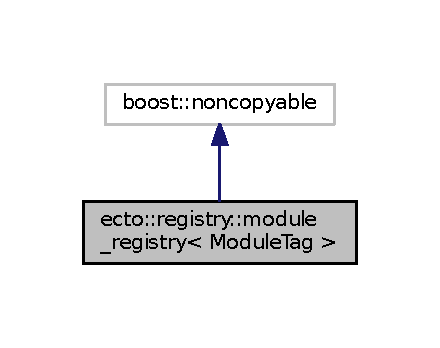
\includegraphics[width=211pt]{structecto_1_1registry_1_1module__registry__inherit__graph}
\end{center}
\end{figure}


Collaboration diagram for ecto\+:\+:registry\+:\+:module\+\_\+registry$<$ Module\+Tag $>$\+:\nopagebreak
\begin{figure}[H]
\begin{center}
\leavevmode
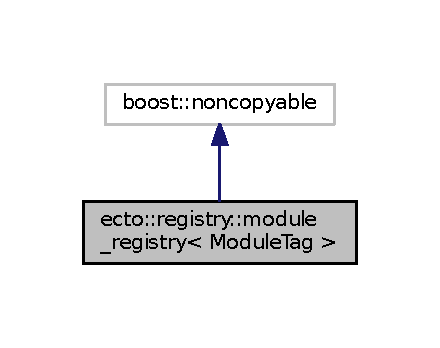
\includegraphics[width=211pt]{structecto_1_1registry_1_1module__registry__coll__graph}
\end{center}
\end{figure}
\subsection*{Public Types}
\begin{DoxyCompactItemize}
\item 
typedef boost\+::function0$<$ void $>$ \hyperlink{structecto_1_1registry_1_1module__registry_a90fc28cbb13d6662b0b8d898985be04e}{nullary\+\_\+fn\+\_\+t}
\end{DoxyCompactItemize}
\subsection*{Public Member Functions}
\begin{DoxyCompactItemize}
\item 
void \hyperlink{structecto_1_1registry_1_1module__registry_aef2549c7e8d6840420041f2231dcdebf}{add} (\hyperlink{structecto_1_1registry_1_1module__registry_a90fc28cbb13d6662b0b8d898985be04e}{nullary\+\_\+fn\+\_\+t} f)
\item 
void \hyperlink{structecto_1_1registry_1_1module__registry_ab8a2255326e085adc04ad180aa1752ec}{go} ()
\end{DoxyCompactItemize}
\subsection*{Static Public Member Functions}
\begin{DoxyCompactItemize}
\item 
static \hyperlink{structecto_1_1registry_1_1module__registry}{module\+\_\+registry} \& \hyperlink{structecto_1_1registry_1_1module__registry_ac968548cf0e11339bf002828e67b857f}{instance} ()
\end{DoxyCompactItemize}
\subsection*{Public Attributes}
\begin{DoxyCompactItemize}
\item 
std\+::vector$<$ \hyperlink{structecto_1_1registry_1_1module__registry_a90fc28cbb13d6662b0b8d898985be04e}{nullary\+\_\+fn\+\_\+t} $>$ \hyperlink{structecto_1_1registry_1_1module__registry_a77ae3e886433428c82d5dbb8039d53f6}{regvec}
\end{DoxyCompactItemize}
\subsection*{Private Member Functions}
\begin{DoxyCompactItemize}
\item 
\hyperlink{structecto_1_1registry_1_1module__registry_aef45ef0e61d967ea203db086f8aa9f65}{module\+\_\+registry} ()
\end{DoxyCompactItemize}


\subsection{Member Typedef Documentation}
\hypertarget{structecto_1_1registry_1_1module__registry_a90fc28cbb13d6662b0b8d898985be04e}{}\index{ecto\+::registry\+::module\+\_\+registry@{ecto\+::registry\+::module\+\_\+registry}!nullary\+\_\+fn\+\_\+t@{nullary\+\_\+fn\+\_\+t}}
\index{nullary\+\_\+fn\+\_\+t@{nullary\+\_\+fn\+\_\+t}!ecto\+::registry\+::module\+\_\+registry@{ecto\+::registry\+::module\+\_\+registry}}
\subsubsection[{nullary\+\_\+fn\+\_\+t}]{\setlength{\rightskip}{0pt plus 5cm}template$<$typename Module\+Tag $>$ typedef boost\+::function0$<$void$>$ {\bf ecto\+::registry\+::module\+\_\+registry}$<$ Module\+Tag $>$\+::{\bf nullary\+\_\+fn\+\_\+t}}\label{structecto_1_1registry_1_1module__registry_a90fc28cbb13d6662b0b8d898985be04e}


\subsection{Constructor \& Destructor Documentation}
\hypertarget{structecto_1_1registry_1_1module__registry_aef45ef0e61d967ea203db086f8aa9f65}{}\index{ecto\+::registry\+::module\+\_\+registry@{ecto\+::registry\+::module\+\_\+registry}!module\+\_\+registry@{module\+\_\+registry}}
\index{module\+\_\+registry@{module\+\_\+registry}!ecto\+::registry\+::module\+\_\+registry@{ecto\+::registry\+::module\+\_\+registry}}
\subsubsection[{module\+\_\+registry}]{\setlength{\rightskip}{0pt plus 5cm}template$<$typename Module\+Tag $>$ {\bf ecto\+::registry\+::module\+\_\+registry}$<$ Module\+Tag $>$\+::{\bf module\+\_\+registry} (
\begin{DoxyParamCaption}
{}
\end{DoxyParamCaption}
)\hspace{0.3cm}{\ttfamily [inline]}, {\ttfamily [private]}}\label{structecto_1_1registry_1_1module__registry_aef45ef0e61d967ea203db086f8aa9f65}


\subsection{Member Function Documentation}
\hypertarget{structecto_1_1registry_1_1module__registry_aef2549c7e8d6840420041f2231dcdebf}{}\index{ecto\+::registry\+::module\+\_\+registry@{ecto\+::registry\+::module\+\_\+registry}!add@{add}}
\index{add@{add}!ecto\+::registry\+::module\+\_\+registry@{ecto\+::registry\+::module\+\_\+registry}}
\subsubsection[{add}]{\setlength{\rightskip}{0pt plus 5cm}template$<$typename Module\+Tag $>$ void {\bf ecto\+::registry\+::module\+\_\+registry}$<$ Module\+Tag $>$\+::add (
\begin{DoxyParamCaption}
\item[{{\bf nullary\+\_\+fn\+\_\+t}}]{f}
\end{DoxyParamCaption}
)\hspace{0.3cm}{\ttfamily [inline]}}\label{structecto_1_1registry_1_1module__registry_aef2549c7e8d6840420041f2231dcdebf}
\hypertarget{structecto_1_1registry_1_1module__registry_ab8a2255326e085adc04ad180aa1752ec}{}\index{ecto\+::registry\+::module\+\_\+registry@{ecto\+::registry\+::module\+\_\+registry}!go@{go}}
\index{go@{go}!ecto\+::registry\+::module\+\_\+registry@{ecto\+::registry\+::module\+\_\+registry}}
\subsubsection[{go}]{\setlength{\rightskip}{0pt plus 5cm}template$<$typename Module\+Tag $>$ void {\bf ecto\+::registry\+::module\+\_\+registry}$<$ Module\+Tag $>$\+::go (
\begin{DoxyParamCaption}
{}
\end{DoxyParamCaption}
)\hspace{0.3cm}{\ttfamily [inline]}}\label{structecto_1_1registry_1_1module__registry_ab8a2255326e085adc04ad180aa1752ec}
\hypertarget{structecto_1_1registry_1_1module__registry_ac968548cf0e11339bf002828e67b857f}{}\index{ecto\+::registry\+::module\+\_\+registry@{ecto\+::registry\+::module\+\_\+registry}!instance@{instance}}
\index{instance@{instance}!ecto\+::registry\+::module\+\_\+registry@{ecto\+::registry\+::module\+\_\+registry}}
\subsubsection[{instance}]{\setlength{\rightskip}{0pt plus 5cm}template$<$typename Module\+Tag $>$ static {\bf module\+\_\+registry}\& {\bf ecto\+::registry\+::module\+\_\+registry}$<$ Module\+Tag $>$\+::instance (
\begin{DoxyParamCaption}
{}
\end{DoxyParamCaption}
)\hspace{0.3cm}{\ttfamily [inline]}, {\ttfamily [static]}}\label{structecto_1_1registry_1_1module__registry_ac968548cf0e11339bf002828e67b857f}


\subsection{Member Data Documentation}
\hypertarget{structecto_1_1registry_1_1module__registry_a77ae3e886433428c82d5dbb8039d53f6}{}\index{ecto\+::registry\+::module\+\_\+registry@{ecto\+::registry\+::module\+\_\+registry}!regvec@{regvec}}
\index{regvec@{regvec}!ecto\+::registry\+::module\+\_\+registry@{ecto\+::registry\+::module\+\_\+registry}}
\subsubsection[{regvec}]{\setlength{\rightskip}{0pt plus 5cm}template$<$typename Module\+Tag $>$ std\+::vector$<${\bf nullary\+\_\+fn\+\_\+t}$>$ {\bf ecto\+::registry\+::module\+\_\+registry}$<$ Module\+Tag $>$\+::regvec}\label{structecto_1_1registry_1_1module__registry_a77ae3e886433428c82d5dbb8039d53f6}


The documentation for this struct was generated from the following file\+:\begin{DoxyCompactItemize}
\item 
/home/vrabaud/workspace/recognition\+\_\+kitchen/src/ecto/include/ecto/\hyperlink{registry_8hpp}{registry.\+hpp}\end{DoxyCompactItemize}

\hypertarget{structecto_1_1tendril_1_1none}{\section{ecto\-:\-:tendril\-:\-:none \-Struct \-Reference}
\label{structecto_1_1tendril_1_1none}\index{ecto\-::tendril\-::none@{ecto\-::tendril\-::none}}
}


\-A none type for tendril when the tendril is uninitialized.  




{\ttfamily \#include $<$tendril.\-hpp$>$}

\subsection*{\-Public \-Member \-Functions}
\begin{DoxyCompactItemize}
\item 
\hyperlink{structecto_1_1tendril_1_1none}{none} \& \hyperlink{structecto_1_1tendril_1_1none_ad595e74035f67c86885f0c37b2e67e3b}{operator=} (const \hyperlink{structecto_1_1tendril_1_1none}{none} \&)
\item 
const \hyperlink{structecto_1_1tendril_1_1none}{none} \& \hyperlink{structecto_1_1tendril_1_1none_a02032ee9d796f16d0db5ec2f531d9f46}{operator=} (const \hyperlink{structecto_1_1tendril_1_1none}{none} \&) const 
\end{DoxyCompactItemize}
\subsection*{\-Friends}
\begin{DoxyCompactItemize}
\item 
bool \hyperlink{structecto_1_1tendril_1_1none_aad4dd147c25c51d5edb1aaaaa2f226ea}{operator==} (const \hyperlink{structecto_1_1tendril_1_1none}{none} \&, const \hyperlink{structecto_1_1tendril_1_1none}{none} \&)
\item 
std\-::ostream \& \hyperlink{structecto_1_1tendril_1_1none_a347ef8229889570e77256cd3b6e8d6b8}{operator$<$$<$} (std\-::ostream \&os, const \hyperlink{structecto_1_1tendril_1_1none}{none} \&)
\end{DoxyCompactItemize}


\subsection{\-Detailed \-Description}
\-A none type for tendril when the tendril is uninitialized. 

\subsection{\-Member \-Function \-Documentation}
\hypertarget{structecto_1_1tendril_1_1none_ad595e74035f67c86885f0c37b2e67e3b}{\index{ecto\-::tendril\-::none@{ecto\-::tendril\-::none}!operator=@{operator=}}
\index{operator=@{operator=}!ecto::tendril::none@{ecto\-::tendril\-::none}}
\subsubsection[{operator=}]{\setlength{\rightskip}{0pt plus 5cm}{\bf none}\& ecto\-::tendril\-::none\-::operator= (
\begin{DoxyParamCaption}
\item[{const {\bf none} \&}]{}
\end{DoxyParamCaption}
)\hspace{0.3cm}{\ttfamily  \mbox{[}inline\mbox{]}}}}\label{structecto_1_1tendril_1_1none_ad595e74035f67c86885f0c37b2e67e3b}
\hypertarget{structecto_1_1tendril_1_1none_a02032ee9d796f16d0db5ec2f531d9f46}{\index{ecto\-::tendril\-::none@{ecto\-::tendril\-::none}!operator=@{operator=}}
\index{operator=@{operator=}!ecto::tendril::none@{ecto\-::tendril\-::none}}
\subsubsection[{operator=}]{\setlength{\rightskip}{0pt plus 5cm}const {\bf none}\& ecto\-::tendril\-::none\-::operator= (
\begin{DoxyParamCaption}
\item[{const {\bf none} \&}]{}
\end{DoxyParamCaption}
) const\hspace{0.3cm}{\ttfamily  \mbox{[}inline\mbox{]}}}}\label{structecto_1_1tendril_1_1none_a02032ee9d796f16d0db5ec2f531d9f46}


\subsection{\-Friends \-And \-Related \-Function \-Documentation}
\hypertarget{structecto_1_1tendril_1_1none_a347ef8229889570e77256cd3b6e8d6b8}{\index{ecto\-::tendril\-::none@{ecto\-::tendril\-::none}!operator$<$$<$@{operator$<$$<$}}
\index{operator$<$$<$@{operator$<$$<$}!ecto::tendril::none@{ecto\-::tendril\-::none}}
\subsubsection[{operator$<$$<$}]{\setlength{\rightskip}{0pt plus 5cm}std\-::ostream\& operator$<$$<$ (
\begin{DoxyParamCaption}
\item[{std\-::ostream \&}]{os, }
\item[{const {\bf none} \&}]{}
\end{DoxyParamCaption}
)\hspace{0.3cm}{\ttfamily  \mbox{[}friend\mbox{]}}}}\label{structecto_1_1tendril_1_1none_a347ef8229889570e77256cd3b6e8d6b8}
\hypertarget{structecto_1_1tendril_1_1none_aad4dd147c25c51d5edb1aaaaa2f226ea}{\index{ecto\-::tendril\-::none@{ecto\-::tendril\-::none}!operator==@{operator==}}
\index{operator==@{operator==}!ecto::tendril::none@{ecto\-::tendril\-::none}}
\subsubsection[{operator==}]{\setlength{\rightskip}{0pt plus 5cm}bool operator== (
\begin{DoxyParamCaption}
\item[{const {\bf none} \&}]{, }
\item[{const {\bf none} \&}]{}
\end{DoxyParamCaption}
)\hspace{0.3cm}{\ttfamily  \mbox{[}friend\mbox{]}}}}\label{structecto_1_1tendril_1_1none_aad4dd147c25c51d5edb1aaaaa2f226ea}


\-The documentation for this struct was generated from the following file\-:\begin{DoxyCompactItemize}
\item 
/home/vrabaud/workspace/recognition\-\_\-kitchen\-\_\-groovy/src/ecto/include/ecto/\hyperlink{tendril_8hpp}{tendril.\-hpp}\end{DoxyCompactItemize}

\hypertarget{classecto_1_1py_1_1nothing__to__lock}{}\section{ecto\+:\+:py\+:\+:nothing\+\_\+to\+\_\+lock Class Reference}
\label{classecto_1_1py_1_1nothing__to__lock}\index{ecto\+::py\+::nothing\+\_\+to\+\_\+lock@{ecto\+::py\+::nothing\+\_\+to\+\_\+lock}}


{\ttfamily \#include $<$gil.\+hpp$>$}



Inheritance diagram for ecto\+:\+:py\+:\+:nothing\+\_\+to\+\_\+lock\+:\nopagebreak
\begin{figure}[H]
\begin{center}
\leavevmode
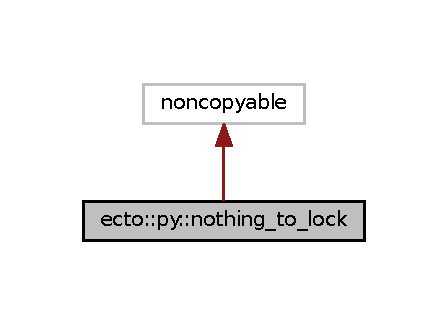
\includegraphics[width=215pt]{classecto_1_1py_1_1nothing__to__lock__inherit__graph}
\end{center}
\end{figure}


Collaboration diagram for ecto\+:\+:py\+:\+:nothing\+\_\+to\+\_\+lock\+:\nopagebreak
\begin{figure}[H]
\begin{center}
\leavevmode
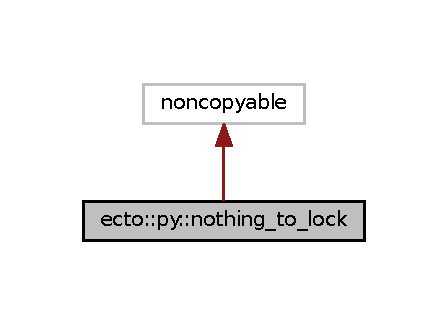
\includegraphics[width=215pt]{classecto_1_1py_1_1nothing__to__lock__coll__graph}
\end{center}
\end{figure}
\subsection*{Public Member Functions}
\begin{DoxyCompactItemize}
\item 
\hyperlink{classecto_1_1py_1_1nothing__to__lock_a277b110e856f61f30f645e4bed50c566}{nothing\+\_\+to\+\_\+lock} ()
\item 
\hyperlink{classecto_1_1py_1_1nothing__to__lock_aa734fa290aeb9aa7de729960aa12df9b}{$\sim$nothing\+\_\+to\+\_\+lock} ()
\end{DoxyCompactItemize}


\subsection{Constructor \& Destructor Documentation}
\index{ecto\+::py\+::nothing\+\_\+to\+\_\+lock@{ecto\+::py\+::nothing\+\_\+to\+\_\+lock}!nothing\+\_\+to\+\_\+lock@{nothing\+\_\+to\+\_\+lock}}
\index{nothing\+\_\+to\+\_\+lock@{nothing\+\_\+to\+\_\+lock}!ecto\+::py\+::nothing\+\_\+to\+\_\+lock@{ecto\+::py\+::nothing\+\_\+to\+\_\+lock}}
\subsubsection[{\texorpdfstring{nothing\+\_\+to\+\_\+lock()}{nothing_to_lock()}}]{\setlength{\rightskip}{0pt plus 5cm}ecto\+::py\+::nothing\+\_\+to\+\_\+lock\+::nothing\+\_\+to\+\_\+lock (
\begin{DoxyParamCaption}
{}
\end{DoxyParamCaption}
)\hspace{0.3cm}{\ttfamily [inline]}}\hypertarget{classecto_1_1py_1_1nothing__to__lock_a277b110e856f61f30f645e4bed50c566}{}\label{classecto_1_1py_1_1nothing__to__lock_a277b110e856f61f30f645e4bed50c566}
\index{ecto\+::py\+::nothing\+\_\+to\+\_\+lock@{ecto\+::py\+::nothing\+\_\+to\+\_\+lock}!````~nothing\+\_\+to\+\_\+lock@{$\sim$nothing\+\_\+to\+\_\+lock}}
\index{````~nothing\+\_\+to\+\_\+lock@{$\sim$nothing\+\_\+to\+\_\+lock}!ecto\+::py\+::nothing\+\_\+to\+\_\+lock@{ecto\+::py\+::nothing\+\_\+to\+\_\+lock}}
\subsubsection[{\texorpdfstring{$\sim$nothing\+\_\+to\+\_\+lock()}{~nothing_to_lock()}}]{\setlength{\rightskip}{0pt plus 5cm}ecto\+::py\+::nothing\+\_\+to\+\_\+lock\+::$\sim$nothing\+\_\+to\+\_\+lock (
\begin{DoxyParamCaption}
{}
\end{DoxyParamCaption}
)\hspace{0.3cm}{\ttfamily [inline]}}\hypertarget{classecto_1_1py_1_1nothing__to__lock_aa734fa290aeb9aa7de729960aa12df9b}{}\label{classecto_1_1py_1_1nothing__to__lock_aa734fa290aeb9aa7de729960aa12df9b}


The documentation for this class was generated from the following file\+:\begin{DoxyCompactItemize}
\item 
/home/vrabaud/workspace/recognition\+\_\+kitchen/src/ecto/include/ecto/python/\hyperlink{gil_8hpp}{gil.\+hpp}\end{DoxyCompactItemize}

\hypertarget{structecto_1_1py_1_1ostream}{}\section{ecto\+:\+:py\+:\+:ostream Struct Reference}
\label{structecto_1_1py_1_1ostream}\index{ecto\+::py\+::ostream@{ecto\+::py\+::ostream}}


{\ttfamily \#include $<$streambuf.\+hpp$>$}



Inheritance diagram for ecto\+:\+:py\+:\+:ostream\+:\nopagebreak
\begin{figure}[H]
\begin{center}
\leavevmode
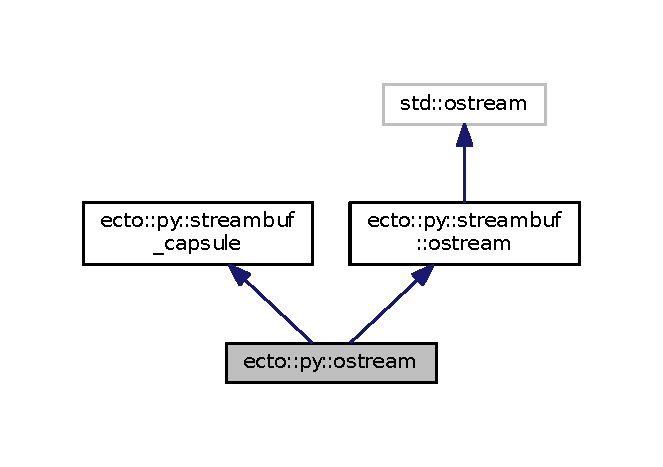
\includegraphics[width=318pt]{structecto_1_1py_1_1ostream__inherit__graph}
\end{center}
\end{figure}


Collaboration diagram for ecto\+:\+:py\+:\+:ostream\+:\nopagebreak
\begin{figure}[H]
\begin{center}
\leavevmode
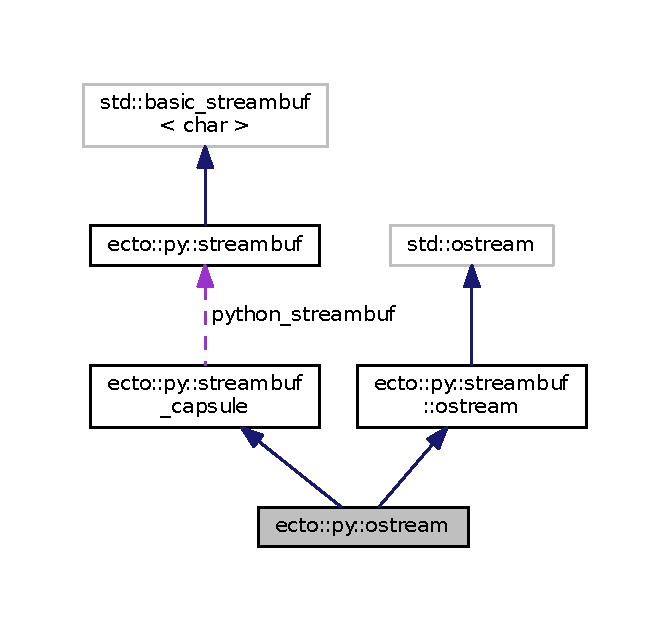
\includegraphics[width=322pt]{structecto_1_1py_1_1ostream__coll__graph}
\end{center}
\end{figure}
\subsection*{Public Member Functions}
\begin{DoxyCompactItemize}
\item 
\hyperlink{structecto_1_1py_1_1ostream_a5fc23212b0b77a69a0c4e7e67133b2c8}{ostream} (bp\+::object \&python\+\_\+file\+\_\+obj, std\+::size\+\_\+t buffer\+\_\+size=0)
\item 
\hyperlink{structecto_1_1py_1_1ostream_a69cba9ec021b14b76fd08d35ea322434}{$\sim$ostream} ()
\end{DoxyCompactItemize}
\subsection*{Additional Inherited Members}


\subsection{Constructor \& Destructor Documentation}
\hypertarget{structecto_1_1py_1_1ostream_a5fc23212b0b77a69a0c4e7e67133b2c8}{}\index{ecto\+::py\+::ostream@{ecto\+::py\+::ostream}!ostream@{ostream}}
\index{ostream@{ostream}!ecto\+::py\+::ostream@{ecto\+::py\+::ostream}}
\subsubsection[{ostream}]{\setlength{\rightskip}{0pt plus 5cm}ecto\+::py\+::ostream\+::ostream (
\begin{DoxyParamCaption}
\item[{bp\+::object \&}]{python\+\_\+file\+\_\+obj, }
\item[{std\+::size\+\_\+t}]{buffer\+\_\+size = {\ttfamily 0}}
\end{DoxyParamCaption}
)\hspace{0.3cm}{\ttfamily [inline]}}\label{structecto_1_1py_1_1ostream_a5fc23212b0b77a69a0c4e7e67133b2c8}
\hypertarget{structecto_1_1py_1_1ostream_a69cba9ec021b14b76fd08d35ea322434}{}\index{ecto\+::py\+::ostream@{ecto\+::py\+::ostream}!````~ostream@{$\sim$ostream}}
\index{````~ostream@{$\sim$ostream}!ecto\+::py\+::ostream@{ecto\+::py\+::ostream}}
\subsubsection[{$\sim$ostream}]{\setlength{\rightskip}{0pt plus 5cm}ecto\+::py\+::ostream\+::$\sim$ostream (
\begin{DoxyParamCaption}
{}
\end{DoxyParamCaption}
)\hspace{0.3cm}{\ttfamily [inline]}}\label{structecto_1_1py_1_1ostream_a69cba9ec021b14b76fd08d35ea322434}


The documentation for this struct was generated from the following file\+:\begin{DoxyCompactItemize}
\item 
/home/vrabaud/workspace/recognition\+\_\+kitchen/src/ecto/include/ecto/python/\hyperlink{streambuf_8hpp}{streambuf.\+hpp}\end{DoxyCompactItemize}

\hypertarget{classecto_1_1py_1_1streambuf_1_1ostream}{}\section{ecto\+:\+:py\+:\+:streambuf\+:\+:ostream Class Reference}
\label{classecto_1_1py_1_1streambuf_1_1ostream}\index{ecto\+::py\+::streambuf\+::ostream@{ecto\+::py\+::streambuf\+::ostream}}


{\ttfamily \#include $<$streambuf.\+hpp$>$}



Inheritance diagram for ecto\+:\+:py\+:\+:streambuf\+:\+:ostream\+:\nopagebreak
\begin{figure}[H]
\begin{center}
\leavevmode
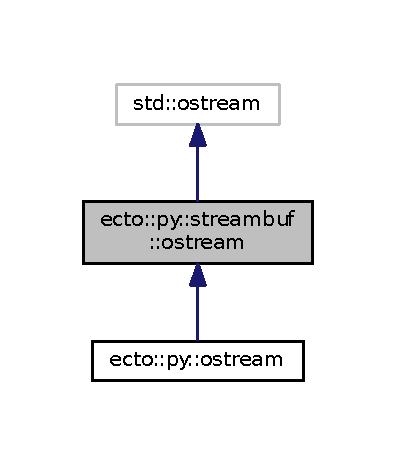
\includegraphics[width=190pt]{classecto_1_1py_1_1streambuf_1_1ostream__inherit__graph}
\end{center}
\end{figure}


Collaboration diagram for ecto\+:\+:py\+:\+:streambuf\+:\+:ostream\+:\nopagebreak
\begin{figure}[H]
\begin{center}
\leavevmode
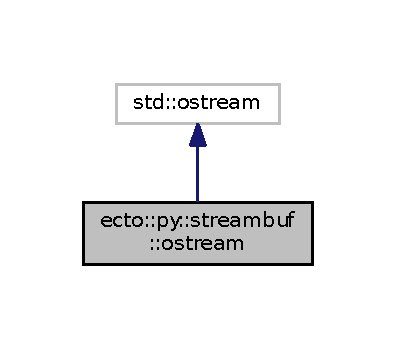
\includegraphics[width=190pt]{classecto_1_1py_1_1streambuf_1_1ostream__coll__graph}
\end{center}
\end{figure}
\subsection*{Public Member Functions}
\begin{DoxyCompactItemize}
\item 
\hyperlink{classecto_1_1py_1_1streambuf_1_1ostream_ab62cdec76b066fa4492b032dd1533bc5}{ostream} (\hyperlink{classecto_1_1py_1_1streambuf}{streambuf} \&buf)
\item 
\hyperlink{classecto_1_1py_1_1streambuf_1_1ostream_abeaab4a21b07a3bbf944d4ce8693a7b5}{$\sim$ostream} ()
\end{DoxyCompactItemize}


\subsection{Constructor \& Destructor Documentation}
\hypertarget{classecto_1_1py_1_1streambuf_1_1ostream_ab62cdec76b066fa4492b032dd1533bc5}{}\index{ecto\+::py\+::streambuf\+::ostream@{ecto\+::py\+::streambuf\+::ostream}!ostream@{ostream}}
\index{ostream@{ostream}!ecto\+::py\+::streambuf\+::ostream@{ecto\+::py\+::streambuf\+::ostream}}
\subsubsection[{ostream}]{\setlength{\rightskip}{0pt plus 5cm}ecto\+::py\+::streambuf\+::ostream\+::ostream (
\begin{DoxyParamCaption}
\item[{{\bf streambuf} \&}]{buf}
\end{DoxyParamCaption}
)\hspace{0.3cm}{\ttfamily [inline]}}\label{classecto_1_1py_1_1streambuf_1_1ostream_ab62cdec76b066fa4492b032dd1533bc5}
\hypertarget{classecto_1_1py_1_1streambuf_1_1ostream_abeaab4a21b07a3bbf944d4ce8693a7b5}{}\index{ecto\+::py\+::streambuf\+::ostream@{ecto\+::py\+::streambuf\+::ostream}!````~ostream@{$\sim$ostream}}
\index{````~ostream@{$\sim$ostream}!ecto\+::py\+::streambuf\+::ostream@{ecto\+::py\+::streambuf\+::ostream}}
\subsubsection[{$\sim$ostream}]{\setlength{\rightskip}{0pt plus 5cm}ecto\+::py\+::streambuf\+::ostream\+::$\sim$ostream (
\begin{DoxyParamCaption}
{}
\end{DoxyParamCaption}
)\hspace{0.3cm}{\ttfamily [inline]}}\label{classecto_1_1py_1_1streambuf_1_1ostream_abeaab4a21b07a3bbf944d4ce8693a7b5}


The documentation for this class was generated from the following file\+:\begin{DoxyCompactItemize}
\item 
/home/vrabaud/workspace/recognition\+\_\+kitchen/src/ecto/include/ecto/python/\hyperlink{streambuf_8hpp}{streambuf.\+hpp}\end{DoxyCompactItemize}

\hypertarget{structecto_1_1plasm}{\section{ecto\-:\-:plasm Struct Reference}
\label{structecto_1_1plasm}\index{ecto\-::plasm@{ecto\-::plasm}}
}


The plasm helps construct the graph structure in ecto. It enforces several invariants that are necessary for scheduling D\-A\-Gs and is used by all the ecto\-::schedulers to enable execution of modules that are connected in the graph.  




{\ttfamily \#include $<$plasm.\-hpp$>$}



Inheritance diagram for ecto\-:\-:plasm\-:\nopagebreak
\begin{figure}[H]
\begin{center}
\leavevmode
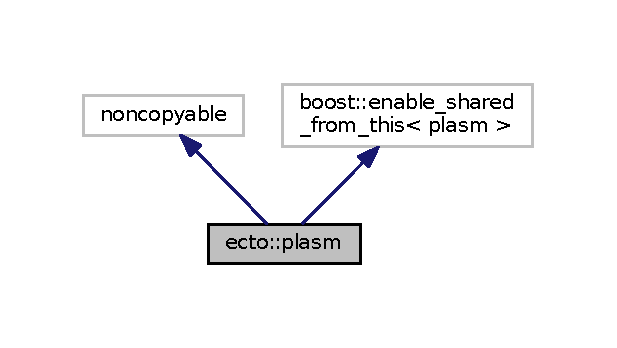
\includegraphics[width=295pt]{structecto_1_1plasm__inherit__graph}
\end{center}
\end{figure}


Collaboration diagram for ecto\-:\-:plasm\-:\nopagebreak
\begin{figure}[H]
\begin{center}
\leavevmode
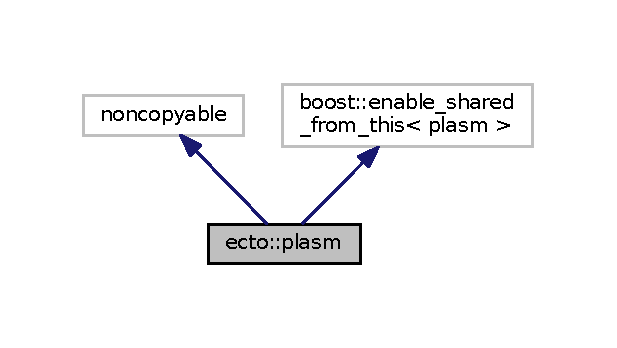
\includegraphics[width=295pt]{structecto_1_1plasm__coll__graph}
\end{center}
\end{figure}
\subsection*{Public Types}
\begin{DoxyCompactItemize}
\item 
typedef boost\-::shared\-\_\-ptr$<$ \hyperlink{structecto_1_1plasm}{plasm} $>$ \hyperlink{structecto_1_1plasm_a899b9da452ab35849f07038c90990ac3}{ptr}
\item 
typedef boost\-::shared\-\_\-ptr\\*
$<$ \hyperlink{structecto_1_1plasm}{plasm} const  $>$ \hyperlink{structecto_1_1plasm_afd3b9e2d4732023ab9e94553e0d66ac4}{cptr}
\item 
typedef boost\-::shared\-\_\-ptr$<$ \hyperlink{structecto_1_1plasm}{plasm} $>$ \hyperlink{structecto_1_1plasm_a899b9da452ab35849f07038c90990ac3}{ptr}
\item 
typedef boost\-::shared\-\_\-ptr\\*
$<$ \hyperlink{structecto_1_1plasm}{plasm} const  $>$ \hyperlink{structecto_1_1plasm_afd3b9e2d4732023ab9e94553e0d66ac4}{cptr}
\end{DoxyCompactItemize}
\subsection*{Public Member Functions}
\begin{DoxyCompactItemize}
\item 
\hyperlink{structecto_1_1plasm_a1d4a2f7e4fa1a4ef839c7ba0316a825c}{plasm} ()
\item 
\hyperlink{structecto_1_1plasm_a3000d2cb042c0875b4d5c38d33763845}{$\sim$plasm} ()
\item 
void \hyperlink{structecto_1_1plasm_a3419c720b1f839cf9b423655cf4de343}{insert} (\hyperlink{namespaceecto_aed1809e82b9229ea81ef9ee3438cf62c}{cell\-\_\-ptr} mod)
\begin{DoxyCompactList}\small\item\em Insert the cell into the graph so that it may be executed by a scheduler. \end{DoxyCompactList}\item 
void \hyperlink{structecto_1_1plasm_a0ca320f5cef8372cfa713fd7991ad3b2}{connect} (\hyperlink{namespaceecto_aed1809e82b9229ea81ef9ee3438cf62c}{cell\-\_\-ptr} from, const std\-::string \&output, \hyperlink{namespaceecto_aed1809e82b9229ea81ef9ee3438cf62c}{cell\-\_\-ptr} to, const std\-::string \&input)
\begin{DoxyCompactList}\small\item\em Connect one cell to another, and populate the graph accordingly. This will throw on a type mismatch. \end{DoxyCompactList}\item 
void \hyperlink{structecto_1_1plasm_a5e187b40ce0a7d7ed9a6859452aed5ca}{disconnect} (\hyperlink{namespaceecto_aed1809e82b9229ea81ef9ee3438cf62c}{cell\-\_\-ptr} from, const std\-::string \&output, \hyperlink{namespaceecto_aed1809e82b9229ea81ef9ee3438cf62c}{cell\-\_\-ptr} to, const std\-::string \&input)
\item 
void \hyperlink{structecto_1_1plasm_a6350e90b6d85a218e7a84183eaed0c18}{viz} (std\-::ostream \&out) const 
\begin{DoxyCompactList}\small\item\em output graphviz to a stream. \end{DoxyCompactList}\item 
std\-::string \hyperlink{structecto_1_1plasm_a4586d90c908123a18dbd3a26c206f63c}{viz} () const 
\begin{DoxyCompactList}\small\item\em Get a std\-::string graphiz of the cell. \end{DoxyCompactList}\item 
void \hyperlink{structecto_1_1plasm_a9554edd5758b8a83ed092a81e249f64a}{check} () const 
\begin{DoxyCompactList}\small\item\em Check that all tags on the graph are satisfied. This will throw on errors in the graph, including, if required inputs are not connected if required outputs are not connected, if there are cycles, etc... \end{DoxyCompactList}\item 
\hyperlink{structecto_1_1graph_1_1graph__t}{graph\-::graph\-\_\-t} \& \hyperlink{structecto_1_1plasm_a4f8de02440afdad0aa395fbaea03399e}{graph} ()
\begin{DoxyCompactList}\small\item\em Get the underlying boost graph that this plasm has constructed. \end{DoxyCompactList}\item 
const \hyperlink{structecto_1_1graph_1_1graph__t}{graph\-::graph\-\_\-t} \& \hyperlink{structecto_1_1plasm_ac6cde6d1d615e85f442ce299fdf0e7a0}{graph} () const 
\item 
std\-::size\-\_\-t \hyperlink{structecto_1_1plasm_aaeeabeb3f78c1a7291eb14e0f705574e}{size} () const 
\begin{DoxyCompactList}\small\item\em Return the number of cells in the plasm (vertices in the graph) \end{DoxyCompactList}\item 
std\-::vector$<$ \hyperlink{namespaceecto_aed1809e82b9229ea81ef9ee3438cf62c}{cell\-\_\-ptr} $>$ \hyperlink{structecto_1_1plasm_aa7724234d631563b10de07030c066e01}{cells} () const 
\begin{DoxyCompactList}\small\item\em Grab a set of all the cells from the plasm. \end{DoxyCompactList}\item 
void \hyperlink{structecto_1_1plasm_a55d56445bd1d09b9422390fb49e81bec}{configure\-\_\-all} ()
\begin{DoxyCompactList}\small\item\em Calls configure on all modules, if configure has not already been called. \end{DoxyCompactList}\item 
void \hyperlink{structecto_1_1plasm_a4419135c6c8dd8bb0cc7f4807a025df2}{activate\-\_\-all} ()
\begin{DoxyCompactList}\small\item\em Calls activate on all modules, if hasn't already been called. \end{DoxyCompactList}\item 
void \hyperlink{structecto_1_1plasm_a6c10f2812f731c3787e5e22bdd80e9bc}{deactivate\-\_\-all} ()
\begin{DoxyCompactList}\small\item\em Calls deactivate on all modules, if it hasn't already been called. \end{DoxyCompactList}\item 
void \hyperlink{structecto_1_1plasm_a992f656fa931efc20d2cf1a97c963cec}{reset\-\_\-ticks} ()
\item 
void \hyperlink{structecto_1_1plasm_ab0fd6bec2e5d8943363fe5aa36c1d676}{save} (std\-::ostream \&) const 
\item 
void \hyperlink{structecto_1_1plasm_a854400c2f46f995731e058c72a547185}{load} (std\-::istream \&)
\item 
\hyperlink{structecto_1_1plasm_a1d4a2f7e4fa1a4ef839c7ba0316a825c}{plasm} ()
\item 
\hyperlink{structecto_1_1plasm_a3000d2cb042c0875b4d5c38d33763845}{$\sim$plasm} ()
\item 
void \hyperlink{structecto_1_1plasm_a3419c720b1f839cf9b423655cf4de343}{insert} (\hyperlink{namespaceecto_aed1809e82b9229ea81ef9ee3438cf62c}{cell\-\_\-ptr} mod)
\begin{DoxyCompactList}\small\item\em Insert the cell into the graph so that it may be executed by a scheduler. \end{DoxyCompactList}\item 
void \hyperlink{structecto_1_1plasm_a0ca320f5cef8372cfa713fd7991ad3b2}{connect} (\hyperlink{namespaceecto_aed1809e82b9229ea81ef9ee3438cf62c}{cell\-\_\-ptr} from, const std\-::string \&output, \hyperlink{namespaceecto_aed1809e82b9229ea81ef9ee3438cf62c}{cell\-\_\-ptr} to, const std\-::string \&input)
\begin{DoxyCompactList}\small\item\em Connect one cell to another, and populate the graph accordingly. This will throw on a type mismatch. \end{DoxyCompactList}\item 
void \hyperlink{structecto_1_1plasm_a5e187b40ce0a7d7ed9a6859452aed5ca}{disconnect} (\hyperlink{namespaceecto_aed1809e82b9229ea81ef9ee3438cf62c}{cell\-\_\-ptr} from, const std\-::string \&output, \hyperlink{namespaceecto_aed1809e82b9229ea81ef9ee3438cf62c}{cell\-\_\-ptr} to, const std\-::string \&input)
\item 
void \hyperlink{structecto_1_1plasm_a6350e90b6d85a218e7a84183eaed0c18}{viz} (std\-::ostream \&out) const 
\begin{DoxyCompactList}\small\item\em output graphviz to a stream. \end{DoxyCompactList}\item 
std\-::string \hyperlink{structecto_1_1plasm_a4586d90c908123a18dbd3a26c206f63c}{viz} () const 
\begin{DoxyCompactList}\small\item\em Get a std\-::string graphiz of the cell. \end{DoxyCompactList}\item 
void \hyperlink{structecto_1_1plasm_a9554edd5758b8a83ed092a81e249f64a}{check} () const 
\begin{DoxyCompactList}\small\item\em Check that all tags on the graph are satisfied. This will throw on errors in the graph, including, if required inputs are not connected if required outputs are not connected, if there are cycles, etc... \end{DoxyCompactList}\item 
\hyperlink{structecto_1_1graph_1_1graph__t}{graph\-::graph\-\_\-t} \& \hyperlink{structecto_1_1plasm_a4f8de02440afdad0aa395fbaea03399e}{graph} ()
\begin{DoxyCompactList}\small\item\em Get the underlying boost graph that this plasm has constructed. \end{DoxyCompactList}\item 
const \hyperlink{structecto_1_1graph_1_1graph__t}{graph\-::graph\-\_\-t} \& \hyperlink{structecto_1_1plasm_ac6cde6d1d615e85f442ce299fdf0e7a0}{graph} () const 
\item 
std\-::size\-\_\-t \hyperlink{structecto_1_1plasm_aaeeabeb3f78c1a7291eb14e0f705574e}{size} () const 
\begin{DoxyCompactList}\small\item\em Return the number of cells in the plasm (vertices in the graph) \end{DoxyCompactList}\item 
std\-::vector$<$ \hyperlink{namespaceecto_aed1809e82b9229ea81ef9ee3438cf62c}{cell\-\_\-ptr} $>$ \hyperlink{structecto_1_1plasm_aa7724234d631563b10de07030c066e01}{cells} () const 
\begin{DoxyCompactList}\small\item\em Grab a set of all the cells from the plasm. \end{DoxyCompactList}\item 
void \hyperlink{structecto_1_1plasm_a55d56445bd1d09b9422390fb49e81bec}{configure\-\_\-all} ()
\begin{DoxyCompactList}\small\item\em Calls configure on all modules, if configure has not already been called. \end{DoxyCompactList}\item 
void \hyperlink{structecto_1_1plasm_a4419135c6c8dd8bb0cc7f4807a025df2}{activate\-\_\-all} ()
\begin{DoxyCompactList}\small\item\em Calls activate on all modules, if hasn't already been called. \end{DoxyCompactList}\item 
void \hyperlink{structecto_1_1plasm_a6c10f2812f731c3787e5e22bdd80e9bc}{deactivate\-\_\-all} ()
\begin{DoxyCompactList}\small\item\em Calls deactivate on all modules, if it hasn't already been called. \end{DoxyCompactList}\item 
void \hyperlink{structecto_1_1plasm_a992f656fa931efc20d2cf1a97c963cec}{reset\-\_\-ticks} ()
\item 
void \hyperlink{structecto_1_1plasm_ab0fd6bec2e5d8943363fe5aa36c1d676}{save} (std\-::ostream \&) const 
\item 
void \hyperlink{structecto_1_1plasm_a854400c2f46f995731e058c72a547185}{load} (std\-::istream \&)
\end{DoxyCompactItemize}
\subsection*{Private Member Functions}
\begin{DoxyCompactItemize}
\item 
{\footnotesize template$<$class Archive $>$ }\\void \hyperlink{structecto_1_1plasm_a420eb464746042e8247a69828e6782af}{save} (Archive \&ar, const unsigned int) const 
\item 
{\footnotesize template$<$class Archive $>$ }\\void \hyperlink{structecto_1_1plasm_ae6540bca37d0980ec24b0b75061e124e}{load} (Archive \&ar, const unsigned int)
\item 
\hyperlink{structecto_1_1plasm_ac443cf0a58324a8003e1c9fd3b49b428}{B\-O\-O\-S\-T\-\_\-\-S\-E\-R\-I\-A\-L\-I\-Z\-A\-T\-I\-O\-N\-\_\-\-S\-P\-L\-I\-T\-\_\-\-M\-E\-M\-B\-E\-R} ()
\item 
{\footnotesize template$<$class Archive $>$ }\\void \hyperlink{structecto_1_1plasm_a420eb464746042e8247a69828e6782af}{save} (Archive \&ar, const unsigned int) const 
\item 
{\footnotesize template$<$class Archive $>$ }\\void \hyperlink{structecto_1_1plasm_ae6540bca37d0980ec24b0b75061e124e}{load} (Archive \&ar, const unsigned int)
\item 
\hyperlink{structecto_1_1plasm_ac443cf0a58324a8003e1c9fd3b49b428}{B\-O\-O\-S\-T\-\_\-\-S\-E\-R\-I\-A\-L\-I\-Z\-A\-T\-I\-O\-N\-\_\-\-S\-P\-L\-I\-T\-\_\-\-M\-E\-M\-B\-E\-R} ()
\end{DoxyCompactItemize}
\subsection*{Private Attributes}
\begin{DoxyCompactItemize}
\item 
boost\-::shared\-\_\-ptr$<$ impl $>$ \hyperlink{structecto_1_1plasm_a3fa8095e74d8f7b36a5fce7ebcd3e79c}{impl\-\_\-}
\item 
bool \hyperlink{structecto_1_1plasm_a8d074da8290587fab0ed04d5cfe3f6b1}{configured}
\end{DoxyCompactItemize}
\subsection*{Friends}
\begin{DoxyCompactItemize}
\item 
class \hyperlink{structecto_1_1plasm_a4305f269960e8ccc92b19b2f0480b16d}{boost\-::serialization\-::access}
\end{DoxyCompactItemize}


\subsection{Detailed Description}
The plasm helps construct the graph structure in ecto. It enforces several invariants that are necessary for scheduling D\-A\-Gs and is used by all the ecto\-::schedulers to enable execution of modules that are connected in the graph. 

\subsection{Member Typedef Documentation}
\hypertarget{structecto_1_1plasm_afd3b9e2d4732023ab9e94553e0d66ac4}{\index{ecto\-::plasm@{ecto\-::plasm}!cptr@{cptr}}
\index{cptr@{cptr}!ecto::plasm@{ecto\-::plasm}}
\subsubsection[{cptr}]{\setlength{\rightskip}{0pt plus 5cm}typedef boost\-::shared\-\_\-ptr$<${\bf plasm} const$>$ {\bf ecto\-::plasm\-::cptr}}}\label{structecto_1_1plasm_afd3b9e2d4732023ab9e94553e0d66ac4}
\hypertarget{structecto_1_1plasm_afd3b9e2d4732023ab9e94553e0d66ac4}{\index{ecto\-::plasm@{ecto\-::plasm}!cptr@{cptr}}
\index{cptr@{cptr}!ecto::plasm@{ecto\-::plasm}}
\subsubsection[{cptr}]{\setlength{\rightskip}{0pt plus 5cm}typedef boost\-::shared\-\_\-ptr$<${\bf plasm} const$>$ {\bf ecto\-::plasm\-::cptr}}}\label{structecto_1_1plasm_afd3b9e2d4732023ab9e94553e0d66ac4}
\hypertarget{structecto_1_1plasm_a899b9da452ab35849f07038c90990ac3}{\index{ecto\-::plasm@{ecto\-::plasm}!ptr@{ptr}}
\index{ptr@{ptr}!ecto::plasm@{ecto\-::plasm}}
\subsubsection[{ptr}]{\setlength{\rightskip}{0pt plus 5cm}typedef boost\-::shared\-\_\-ptr$<${\bf plasm}$>$ {\bf ecto\-::plasm\-::ptr}}}\label{structecto_1_1plasm_a899b9da452ab35849f07038c90990ac3}
\hypertarget{structecto_1_1plasm_a899b9da452ab35849f07038c90990ac3}{\index{ecto\-::plasm@{ecto\-::plasm}!ptr@{ptr}}
\index{ptr@{ptr}!ecto::plasm@{ecto\-::plasm}}
\subsubsection[{ptr}]{\setlength{\rightskip}{0pt plus 5cm}typedef boost\-::shared\-\_\-ptr$<${\bf plasm}$>$ {\bf ecto\-::plasm\-::ptr}}}\label{structecto_1_1plasm_a899b9da452ab35849f07038c90990ac3}


\subsection{Constructor \& Destructor Documentation}
\hypertarget{structecto_1_1plasm_a1d4a2f7e4fa1a4ef839c7ba0316a825c}{\index{ecto\-::plasm@{ecto\-::plasm}!plasm@{plasm}}
\index{plasm@{plasm}!ecto::plasm@{ecto\-::plasm}}
\subsubsection[{plasm}]{\setlength{\rightskip}{0pt plus 5cm}ecto\-::plasm\-::plasm (
\begin{DoxyParamCaption}
{}
\end{DoxyParamCaption}
)}}\label{structecto_1_1plasm_a1d4a2f7e4fa1a4ef839c7ba0316a825c}
\hypertarget{structecto_1_1plasm_a3000d2cb042c0875b4d5c38d33763845}{\index{ecto\-::plasm@{ecto\-::plasm}!$\sim$plasm@{$\sim$plasm}}
\index{$\sim$plasm@{$\sim$plasm}!ecto::plasm@{ecto\-::plasm}}
\subsubsection[{$\sim$plasm}]{\setlength{\rightskip}{0pt plus 5cm}ecto\-::plasm\-::$\sim$plasm (
\begin{DoxyParamCaption}
{}
\end{DoxyParamCaption}
)}}\label{structecto_1_1plasm_a3000d2cb042c0875b4d5c38d33763845}
\hypertarget{structecto_1_1plasm_a1d4a2f7e4fa1a4ef839c7ba0316a825c}{\index{ecto\-::plasm@{ecto\-::plasm}!plasm@{plasm}}
\index{plasm@{plasm}!ecto::plasm@{ecto\-::plasm}}
\subsubsection[{plasm}]{\setlength{\rightskip}{0pt plus 5cm}ecto\-::plasm\-::plasm (
\begin{DoxyParamCaption}
{}
\end{DoxyParamCaption}
)}}\label{structecto_1_1plasm_a1d4a2f7e4fa1a4ef839c7ba0316a825c}
\hypertarget{structecto_1_1plasm_a3000d2cb042c0875b4d5c38d33763845}{\index{ecto\-::plasm@{ecto\-::plasm}!$\sim$plasm@{$\sim$plasm}}
\index{$\sim$plasm@{$\sim$plasm}!ecto::plasm@{ecto\-::plasm}}
\subsubsection[{$\sim$plasm}]{\setlength{\rightskip}{0pt plus 5cm}ecto\-::plasm\-::$\sim$plasm (
\begin{DoxyParamCaption}
{}
\end{DoxyParamCaption}
)}}\label{structecto_1_1plasm_a3000d2cb042c0875b4d5c38d33763845}


\subsection{Member Function Documentation}
\hypertarget{structecto_1_1plasm_a4419135c6c8dd8bb0cc7f4807a025df2}{\index{ecto\-::plasm@{ecto\-::plasm}!activate\-\_\-all@{activate\-\_\-all}}
\index{activate\-\_\-all@{activate\-\_\-all}!ecto::plasm@{ecto\-::plasm}}
\subsubsection[{activate\-\_\-all}]{\setlength{\rightskip}{0pt plus 5cm}void ecto\-::plasm\-::activate\-\_\-all (
\begin{DoxyParamCaption}
{}
\end{DoxyParamCaption}
)}}\label{structecto_1_1plasm_a4419135c6c8dd8bb0cc7f4807a025df2}


Calls activate on all modules, if hasn't already been called. 

\hypertarget{structecto_1_1plasm_a4419135c6c8dd8bb0cc7f4807a025df2}{\index{ecto\-::plasm@{ecto\-::plasm}!activate\-\_\-all@{activate\-\_\-all}}
\index{activate\-\_\-all@{activate\-\_\-all}!ecto::plasm@{ecto\-::plasm}}
\subsubsection[{activate\-\_\-all}]{\setlength{\rightskip}{0pt plus 5cm}void ecto\-::plasm\-::activate\-\_\-all (
\begin{DoxyParamCaption}
{}
\end{DoxyParamCaption}
)}}\label{structecto_1_1plasm_a4419135c6c8dd8bb0cc7f4807a025df2}


Calls activate on all modules, if hasn't already been called. 

\hypertarget{structecto_1_1plasm_ac443cf0a58324a8003e1c9fd3b49b428}{\index{ecto\-::plasm@{ecto\-::plasm}!B\-O\-O\-S\-T\-\_\-\-S\-E\-R\-I\-A\-L\-I\-Z\-A\-T\-I\-O\-N\-\_\-\-S\-P\-L\-I\-T\-\_\-\-M\-E\-M\-B\-E\-R@{B\-O\-O\-S\-T\-\_\-\-S\-E\-R\-I\-A\-L\-I\-Z\-A\-T\-I\-O\-N\-\_\-\-S\-P\-L\-I\-T\-\_\-\-M\-E\-M\-B\-E\-R}}
\index{B\-O\-O\-S\-T\-\_\-\-S\-E\-R\-I\-A\-L\-I\-Z\-A\-T\-I\-O\-N\-\_\-\-S\-P\-L\-I\-T\-\_\-\-M\-E\-M\-B\-E\-R@{B\-O\-O\-S\-T\-\_\-\-S\-E\-R\-I\-A\-L\-I\-Z\-A\-T\-I\-O\-N\-\_\-\-S\-P\-L\-I\-T\-\_\-\-M\-E\-M\-B\-E\-R}!ecto::plasm@{ecto\-::plasm}}
\subsubsection[{B\-O\-O\-S\-T\-\_\-\-S\-E\-R\-I\-A\-L\-I\-Z\-A\-T\-I\-O\-N\-\_\-\-S\-P\-L\-I\-T\-\_\-\-M\-E\-M\-B\-E\-R}]{\setlength{\rightskip}{0pt plus 5cm}ecto\-::plasm\-::\-B\-O\-O\-S\-T\-\_\-\-S\-E\-R\-I\-A\-L\-I\-Z\-A\-T\-I\-O\-N\-\_\-\-S\-P\-L\-I\-T\-\_\-\-M\-E\-M\-B\-E\-R (
\begin{DoxyParamCaption}
{}
\end{DoxyParamCaption}
)\hspace{0.3cm}{\ttfamily [private]}}}\label{structecto_1_1plasm_ac443cf0a58324a8003e1c9fd3b49b428}
\hypertarget{structecto_1_1plasm_ac443cf0a58324a8003e1c9fd3b49b428}{\index{ecto\-::plasm@{ecto\-::plasm}!B\-O\-O\-S\-T\-\_\-\-S\-E\-R\-I\-A\-L\-I\-Z\-A\-T\-I\-O\-N\-\_\-\-S\-P\-L\-I\-T\-\_\-\-M\-E\-M\-B\-E\-R@{B\-O\-O\-S\-T\-\_\-\-S\-E\-R\-I\-A\-L\-I\-Z\-A\-T\-I\-O\-N\-\_\-\-S\-P\-L\-I\-T\-\_\-\-M\-E\-M\-B\-E\-R}}
\index{B\-O\-O\-S\-T\-\_\-\-S\-E\-R\-I\-A\-L\-I\-Z\-A\-T\-I\-O\-N\-\_\-\-S\-P\-L\-I\-T\-\_\-\-M\-E\-M\-B\-E\-R@{B\-O\-O\-S\-T\-\_\-\-S\-E\-R\-I\-A\-L\-I\-Z\-A\-T\-I\-O\-N\-\_\-\-S\-P\-L\-I\-T\-\_\-\-M\-E\-M\-B\-E\-R}!ecto::plasm@{ecto\-::plasm}}
\subsubsection[{B\-O\-O\-S\-T\-\_\-\-S\-E\-R\-I\-A\-L\-I\-Z\-A\-T\-I\-O\-N\-\_\-\-S\-P\-L\-I\-T\-\_\-\-M\-E\-M\-B\-E\-R}]{\setlength{\rightskip}{0pt plus 5cm}ecto\-::plasm\-::\-B\-O\-O\-S\-T\-\_\-\-S\-E\-R\-I\-A\-L\-I\-Z\-A\-T\-I\-O\-N\-\_\-\-S\-P\-L\-I\-T\-\_\-\-M\-E\-M\-B\-E\-R (
\begin{DoxyParamCaption}
{}
\end{DoxyParamCaption}
)\hspace{0.3cm}{\ttfamily [private]}}}\label{structecto_1_1plasm_ac443cf0a58324a8003e1c9fd3b49b428}
\hypertarget{structecto_1_1plasm_aa7724234d631563b10de07030c066e01}{\index{ecto\-::plasm@{ecto\-::plasm}!cells@{cells}}
\index{cells@{cells}!ecto::plasm@{ecto\-::plasm}}
\subsubsection[{cells}]{\setlength{\rightskip}{0pt plus 5cm}std\-::vector$<${\bf cell\-\_\-ptr}$>$ ecto\-::plasm\-::cells (
\begin{DoxyParamCaption}
{}
\end{DoxyParamCaption}
) const}}\label{structecto_1_1plasm_aa7724234d631563b10de07030c066e01}


Grab a set of all the cells from the plasm. 

\begin{DoxyReturn}{Returns}
a set of cells. 
\end{DoxyReturn}
\hypertarget{structecto_1_1plasm_aa7724234d631563b10de07030c066e01}{\index{ecto\-::plasm@{ecto\-::plasm}!cells@{cells}}
\index{cells@{cells}!ecto::plasm@{ecto\-::plasm}}
\subsubsection[{cells}]{\setlength{\rightskip}{0pt plus 5cm}std\-::vector$<${\bf cell\-\_\-ptr}$>$ ecto\-::plasm\-::cells (
\begin{DoxyParamCaption}
{}
\end{DoxyParamCaption}
) const}}\label{structecto_1_1plasm_aa7724234d631563b10de07030c066e01}


Grab a set of all the cells from the plasm. 

\begin{DoxyReturn}{Returns}
a set of cells. 
\end{DoxyReturn}
\hypertarget{structecto_1_1plasm_a9554edd5758b8a83ed092a81e249f64a}{\index{ecto\-::plasm@{ecto\-::plasm}!check@{check}}
\index{check@{check}!ecto::plasm@{ecto\-::plasm}}
\subsubsection[{check}]{\setlength{\rightskip}{0pt plus 5cm}void ecto\-::plasm\-::check (
\begin{DoxyParamCaption}
{}
\end{DoxyParamCaption}
) const}}\label{structecto_1_1plasm_a9554edd5758b8a83ed092a81e249f64a}


Check that all tags on the graph are satisfied. This will throw on errors in the graph, including, if required inputs are not connected if required outputs are not connected, if there are cycles, etc... 

\hypertarget{structecto_1_1plasm_a9554edd5758b8a83ed092a81e249f64a}{\index{ecto\-::plasm@{ecto\-::plasm}!check@{check}}
\index{check@{check}!ecto::plasm@{ecto\-::plasm}}
\subsubsection[{check}]{\setlength{\rightskip}{0pt plus 5cm}void ecto\-::plasm\-::check (
\begin{DoxyParamCaption}
{}
\end{DoxyParamCaption}
) const}}\label{structecto_1_1plasm_a9554edd5758b8a83ed092a81e249f64a}


Check that all tags on the graph are satisfied. This will throw on errors in the graph, including, if required inputs are not connected if required outputs are not connected, if there are cycles, etc... 

\hypertarget{structecto_1_1plasm_a55d56445bd1d09b9422390fb49e81bec}{\index{ecto\-::plasm@{ecto\-::plasm}!configure\-\_\-all@{configure\-\_\-all}}
\index{configure\-\_\-all@{configure\-\_\-all}!ecto::plasm@{ecto\-::plasm}}
\subsubsection[{configure\-\_\-all}]{\setlength{\rightskip}{0pt plus 5cm}void ecto\-::plasm\-::configure\-\_\-all (
\begin{DoxyParamCaption}
{}
\end{DoxyParamCaption}
)}}\label{structecto_1_1plasm_a55d56445bd1d09b9422390fb49e81bec}


Calls configure on all modules, if configure has not already been called. 

\hypertarget{structecto_1_1plasm_a55d56445bd1d09b9422390fb49e81bec}{\index{ecto\-::plasm@{ecto\-::plasm}!configure\-\_\-all@{configure\-\_\-all}}
\index{configure\-\_\-all@{configure\-\_\-all}!ecto::plasm@{ecto\-::plasm}}
\subsubsection[{configure\-\_\-all}]{\setlength{\rightskip}{0pt plus 5cm}void ecto\-::plasm\-::configure\-\_\-all (
\begin{DoxyParamCaption}
{}
\end{DoxyParamCaption}
)}}\label{structecto_1_1plasm_a55d56445bd1d09b9422390fb49e81bec}


Calls configure on all modules, if configure has not already been called. 

\hypertarget{structecto_1_1plasm_a0ca320f5cef8372cfa713fd7991ad3b2}{\index{ecto\-::plasm@{ecto\-::plasm}!connect@{connect}}
\index{connect@{connect}!ecto::plasm@{ecto\-::plasm}}
\subsubsection[{connect}]{\setlength{\rightskip}{0pt plus 5cm}void ecto\-::plasm\-::connect (
\begin{DoxyParamCaption}
\item[{{\bf cell\-\_\-ptr}}]{from, }
\item[{const std\-::string \&}]{output, }
\item[{{\bf cell\-\_\-ptr}}]{to, }
\item[{const std\-::string \&}]{input}
\end{DoxyParamCaption}
)}}\label{structecto_1_1plasm_a0ca320f5cef8372cfa713fd7991ad3b2}


Connect one cell to another, and populate the graph accordingly. This will throw on a type mismatch. 


\begin{DoxyParams}{Parameters}
{\em from} & The from cell \\
\hline
{\em output} & The output key of the from cell \\
\hline
{\em to} & The to cell \\
\hline
{\em input} & The input key from the to cell. \\
\hline
\end{DoxyParams}
\hypertarget{structecto_1_1plasm_a0ca320f5cef8372cfa713fd7991ad3b2}{\index{ecto\-::plasm@{ecto\-::plasm}!connect@{connect}}
\index{connect@{connect}!ecto::plasm@{ecto\-::plasm}}
\subsubsection[{connect}]{\setlength{\rightskip}{0pt plus 5cm}void ecto\-::plasm\-::connect (
\begin{DoxyParamCaption}
\item[{{\bf cell\-\_\-ptr}}]{from, }
\item[{const std\-::string \&}]{output, }
\item[{{\bf cell\-\_\-ptr}}]{to, }
\item[{const std\-::string \&}]{input}
\end{DoxyParamCaption}
)}}\label{structecto_1_1plasm_a0ca320f5cef8372cfa713fd7991ad3b2}


Connect one cell to another, and populate the graph accordingly. This will throw on a type mismatch. 


\begin{DoxyParams}{Parameters}
{\em from} & The from cell \\
\hline
{\em output} & The output key of the from cell \\
\hline
{\em to} & The to cell \\
\hline
{\em input} & The input key from the to cell. \\
\hline
\end{DoxyParams}
\hypertarget{structecto_1_1plasm_a6c10f2812f731c3787e5e22bdd80e9bc}{\index{ecto\-::plasm@{ecto\-::plasm}!deactivate\-\_\-all@{deactivate\-\_\-all}}
\index{deactivate\-\_\-all@{deactivate\-\_\-all}!ecto::plasm@{ecto\-::plasm}}
\subsubsection[{deactivate\-\_\-all}]{\setlength{\rightskip}{0pt plus 5cm}void ecto\-::plasm\-::deactivate\-\_\-all (
\begin{DoxyParamCaption}
{}
\end{DoxyParamCaption}
)}}\label{structecto_1_1plasm_a6c10f2812f731c3787e5e22bdd80e9bc}


Calls deactivate on all modules, if it hasn't already been called. 

\hypertarget{structecto_1_1plasm_a6c10f2812f731c3787e5e22bdd80e9bc}{\index{ecto\-::plasm@{ecto\-::plasm}!deactivate\-\_\-all@{deactivate\-\_\-all}}
\index{deactivate\-\_\-all@{deactivate\-\_\-all}!ecto::plasm@{ecto\-::plasm}}
\subsubsection[{deactivate\-\_\-all}]{\setlength{\rightskip}{0pt plus 5cm}void ecto\-::plasm\-::deactivate\-\_\-all (
\begin{DoxyParamCaption}
{}
\end{DoxyParamCaption}
)}}\label{structecto_1_1plasm_a6c10f2812f731c3787e5e22bdd80e9bc}


Calls deactivate on all modules, if it hasn't already been called. 

\hypertarget{structecto_1_1plasm_a5e187b40ce0a7d7ed9a6859452aed5ca}{\index{ecto\-::plasm@{ecto\-::plasm}!disconnect@{disconnect}}
\index{disconnect@{disconnect}!ecto::plasm@{ecto\-::plasm}}
\subsubsection[{disconnect}]{\setlength{\rightskip}{0pt plus 5cm}void ecto\-::plasm\-::disconnect (
\begin{DoxyParamCaption}
\item[{{\bf cell\-\_\-ptr}}]{from, }
\item[{const std\-::string \&}]{output, }
\item[{{\bf cell\-\_\-ptr}}]{to, }
\item[{const std\-::string \&}]{input}
\end{DoxyParamCaption}
)}}\label{structecto_1_1plasm_a5e187b40ce0a7d7ed9a6859452aed5ca}
Disconnect a tendril from another tendril.


\begin{DoxyParams}{Parameters}
{\em from} & \\
\hline
{\em output} & \\
\hline
{\em to} & \\
\hline
{\em input} & \\
\hline
\end{DoxyParams}
\hypertarget{structecto_1_1plasm_a5e187b40ce0a7d7ed9a6859452aed5ca}{\index{ecto\-::plasm@{ecto\-::plasm}!disconnect@{disconnect}}
\index{disconnect@{disconnect}!ecto::plasm@{ecto\-::plasm}}
\subsubsection[{disconnect}]{\setlength{\rightskip}{0pt plus 5cm}void ecto\-::plasm\-::disconnect (
\begin{DoxyParamCaption}
\item[{{\bf cell\-\_\-ptr}}]{from, }
\item[{const std\-::string \&}]{output, }
\item[{{\bf cell\-\_\-ptr}}]{to, }
\item[{const std\-::string \&}]{input}
\end{DoxyParamCaption}
)}}\label{structecto_1_1plasm_a5e187b40ce0a7d7ed9a6859452aed5ca}
Disconnect a tendril from another tendril.


\begin{DoxyParams}{Parameters}
{\em from} & \\
\hline
{\em output} & \\
\hline
{\em to} & \\
\hline
{\em input} & \\
\hline
\end{DoxyParams}
\hypertarget{structecto_1_1plasm_a4f8de02440afdad0aa395fbaea03399e}{\index{ecto\-::plasm@{ecto\-::plasm}!graph@{graph}}
\index{graph@{graph}!ecto::plasm@{ecto\-::plasm}}
\subsubsection[{graph}]{\setlength{\rightskip}{0pt plus 5cm}{\bf graph\-::graph\-\_\-t}\& ecto\-::plasm\-::graph (
\begin{DoxyParamCaption}
{}
\end{DoxyParamCaption}
)}}\label{structecto_1_1plasm_a4f8de02440afdad0aa395fbaea03399e}


Get the underlying boost graph that this plasm has constructed. 

\begin{DoxyReturn}{Returns}

\end{DoxyReturn}
\hypertarget{structecto_1_1plasm_a4f8de02440afdad0aa395fbaea03399e}{\index{ecto\-::plasm@{ecto\-::plasm}!graph@{graph}}
\index{graph@{graph}!ecto::plasm@{ecto\-::plasm}}
\subsubsection[{graph}]{\setlength{\rightskip}{0pt plus 5cm}{\bf graph\-::graph\-\_\-t}\& ecto\-::plasm\-::graph (
\begin{DoxyParamCaption}
{}
\end{DoxyParamCaption}
)}}\label{structecto_1_1plasm_a4f8de02440afdad0aa395fbaea03399e}


Get the underlying boost graph that this plasm has constructed. 

\begin{DoxyReturn}{Returns}

\end{DoxyReturn}
\hypertarget{structecto_1_1plasm_ac6cde6d1d615e85f442ce299fdf0e7a0}{\index{ecto\-::plasm@{ecto\-::plasm}!graph@{graph}}
\index{graph@{graph}!ecto::plasm@{ecto\-::plasm}}
\subsubsection[{graph}]{\setlength{\rightskip}{0pt plus 5cm}const {\bf graph\-::graph\-\_\-t}\& ecto\-::plasm\-::graph (
\begin{DoxyParamCaption}
{}
\end{DoxyParamCaption}
) const}}\label{structecto_1_1plasm_ac6cde6d1d615e85f442ce299fdf0e7a0}
\hypertarget{structecto_1_1plasm_ac6cde6d1d615e85f442ce299fdf0e7a0}{\index{ecto\-::plasm@{ecto\-::plasm}!graph@{graph}}
\index{graph@{graph}!ecto::plasm@{ecto\-::plasm}}
\subsubsection[{graph}]{\setlength{\rightskip}{0pt plus 5cm}const {\bf graph\-::graph\-\_\-t}\& ecto\-::plasm\-::graph (
\begin{DoxyParamCaption}
{}
\end{DoxyParamCaption}
) const}}\label{structecto_1_1plasm_ac6cde6d1d615e85f442ce299fdf0e7a0}
\hypertarget{structecto_1_1plasm_a3419c720b1f839cf9b423655cf4de343}{\index{ecto\-::plasm@{ecto\-::plasm}!insert@{insert}}
\index{insert@{insert}!ecto::plasm@{ecto\-::plasm}}
\subsubsection[{insert}]{\setlength{\rightskip}{0pt plus 5cm}void ecto\-::plasm\-::insert (
\begin{DoxyParamCaption}
\item[{{\bf cell\-\_\-ptr}}]{mod}
\end{DoxyParamCaption}
)}}\label{structecto_1_1plasm_a3419c720b1f839cf9b423655cf4de343}


Insert the cell into the graph so that it may be executed by a scheduler. 


\begin{DoxyParams}{Parameters}
{\em mod} & The cell to insert into the graph. \\
\hline
\end{DoxyParams}
\hypertarget{structecto_1_1plasm_a3419c720b1f839cf9b423655cf4de343}{\index{ecto\-::plasm@{ecto\-::plasm}!insert@{insert}}
\index{insert@{insert}!ecto::plasm@{ecto\-::plasm}}
\subsubsection[{insert}]{\setlength{\rightskip}{0pt plus 5cm}void ecto\-::plasm\-::insert (
\begin{DoxyParamCaption}
\item[{{\bf cell\-\_\-ptr}}]{mod}
\end{DoxyParamCaption}
)}}\label{structecto_1_1plasm_a3419c720b1f839cf9b423655cf4de343}


Insert the cell into the graph so that it may be executed by a scheduler. 


\begin{DoxyParams}{Parameters}
{\em mod} & The cell to insert into the graph. \\
\hline
\end{DoxyParams}
\hypertarget{structecto_1_1plasm_a854400c2f46f995731e058c72a547185}{\index{ecto\-::plasm@{ecto\-::plasm}!load@{load}}
\index{load@{load}!ecto::plasm@{ecto\-::plasm}}
\subsubsection[{load}]{\setlength{\rightskip}{0pt plus 5cm}void ecto\-::plasm\-::load (
\begin{DoxyParamCaption}
\item[{std\-::istream \&}]{}
\end{DoxyParamCaption}
)}}\label{structecto_1_1plasm_a854400c2f46f995731e058c72a547185}
\hypertarget{structecto_1_1plasm_a854400c2f46f995731e058c72a547185}{\index{ecto\-::plasm@{ecto\-::plasm}!load@{load}}
\index{load@{load}!ecto::plasm@{ecto\-::plasm}}
\subsubsection[{load}]{\setlength{\rightskip}{0pt plus 5cm}void ecto\-::plasm\-::load (
\begin{DoxyParamCaption}
\item[{std\-::istream \&}]{}
\end{DoxyParamCaption}
)}}\label{structecto_1_1plasm_a854400c2f46f995731e058c72a547185}
\hypertarget{structecto_1_1plasm_ae6540bca37d0980ec24b0b75061e124e}{\index{ecto\-::plasm@{ecto\-::plasm}!load@{load}}
\index{load@{load}!ecto::plasm@{ecto\-::plasm}}
\subsubsection[{load}]{\setlength{\rightskip}{0pt plus 5cm}template$<$class Archive $>$ void ecto\-::plasm\-::load (
\begin{DoxyParamCaption}
\item[{Archive \&}]{ar, }
\item[{const unsigned}]{int}
\end{DoxyParamCaption}
)\hspace{0.3cm}{\ttfamily [private]}}}\label{structecto_1_1plasm_ae6540bca37d0980ec24b0b75061e124e}
\hypertarget{structecto_1_1plasm_ae6540bca37d0980ec24b0b75061e124e}{\index{ecto\-::plasm@{ecto\-::plasm}!load@{load}}
\index{load@{load}!ecto::plasm@{ecto\-::plasm}}
\subsubsection[{load}]{\setlength{\rightskip}{0pt plus 5cm}template$<$class Archive $>$ void ecto\-::plasm\-::load (
\begin{DoxyParamCaption}
\item[{Archive \&}]{ar, }
\item[{const unsigned}]{int}
\end{DoxyParamCaption}
)\hspace{0.3cm}{\ttfamily [private]}}}\label{structecto_1_1plasm_ae6540bca37d0980ec24b0b75061e124e}
\hypertarget{structecto_1_1plasm_a992f656fa931efc20d2cf1a97c963cec}{\index{ecto\-::plasm@{ecto\-::plasm}!reset\-\_\-ticks@{reset\-\_\-ticks}}
\index{reset\-\_\-ticks@{reset\-\_\-ticks}!ecto::plasm@{ecto\-::plasm}}
\subsubsection[{reset\-\_\-ticks}]{\setlength{\rightskip}{0pt plus 5cm}void ecto\-::plasm\-::reset\-\_\-ticks (
\begin{DoxyParamCaption}
{}
\end{DoxyParamCaption}
)}}\label{structecto_1_1plasm_a992f656fa931efc20d2cf1a97c963cec}
\hypertarget{structecto_1_1plasm_a992f656fa931efc20d2cf1a97c963cec}{\index{ecto\-::plasm@{ecto\-::plasm}!reset\-\_\-ticks@{reset\-\_\-ticks}}
\index{reset\-\_\-ticks@{reset\-\_\-ticks}!ecto::plasm@{ecto\-::plasm}}
\subsubsection[{reset\-\_\-ticks}]{\setlength{\rightskip}{0pt plus 5cm}void ecto\-::plasm\-::reset\-\_\-ticks (
\begin{DoxyParamCaption}
{}
\end{DoxyParamCaption}
)}}\label{structecto_1_1plasm_a992f656fa931efc20d2cf1a97c963cec}
\hypertarget{structecto_1_1plasm_ab0fd6bec2e5d8943363fe5aa36c1d676}{\index{ecto\-::plasm@{ecto\-::plasm}!save@{save}}
\index{save@{save}!ecto::plasm@{ecto\-::plasm}}
\subsubsection[{save}]{\setlength{\rightskip}{0pt plus 5cm}void ecto\-::plasm\-::save (
\begin{DoxyParamCaption}
\item[{std\-::ostream \&}]{}
\end{DoxyParamCaption}
) const}}\label{structecto_1_1plasm_ab0fd6bec2e5d8943363fe5aa36c1d676}
\hypertarget{structecto_1_1plasm_ab0fd6bec2e5d8943363fe5aa36c1d676}{\index{ecto\-::plasm@{ecto\-::plasm}!save@{save}}
\index{save@{save}!ecto::plasm@{ecto\-::plasm}}
\subsubsection[{save}]{\setlength{\rightskip}{0pt plus 5cm}void ecto\-::plasm\-::save (
\begin{DoxyParamCaption}
\item[{std\-::ostream \&}]{}
\end{DoxyParamCaption}
) const}}\label{structecto_1_1plasm_ab0fd6bec2e5d8943363fe5aa36c1d676}
\hypertarget{structecto_1_1plasm_a420eb464746042e8247a69828e6782af}{\index{ecto\-::plasm@{ecto\-::plasm}!save@{save}}
\index{save@{save}!ecto::plasm@{ecto\-::plasm}}
\subsubsection[{save}]{\setlength{\rightskip}{0pt plus 5cm}template$<$class Archive $>$ void ecto\-::plasm\-::save (
\begin{DoxyParamCaption}
\item[{Archive \&}]{ar, }
\item[{const unsigned}]{int}
\end{DoxyParamCaption}
) const\hspace{0.3cm}{\ttfamily [private]}}}\label{structecto_1_1plasm_a420eb464746042e8247a69828e6782af}
\hypertarget{structecto_1_1plasm_a420eb464746042e8247a69828e6782af}{\index{ecto\-::plasm@{ecto\-::plasm}!save@{save}}
\index{save@{save}!ecto::plasm@{ecto\-::plasm}}
\subsubsection[{save}]{\setlength{\rightskip}{0pt plus 5cm}template$<$class Archive $>$ void ecto\-::plasm\-::save (
\begin{DoxyParamCaption}
\item[{Archive \&}]{ar, }
\item[{const unsigned}]{int}
\end{DoxyParamCaption}
) const\hspace{0.3cm}{\ttfamily [private]}}}\label{structecto_1_1plasm_a420eb464746042e8247a69828e6782af}
\hypertarget{structecto_1_1plasm_aaeeabeb3f78c1a7291eb14e0f705574e}{\index{ecto\-::plasm@{ecto\-::plasm}!size@{size}}
\index{size@{size}!ecto::plasm@{ecto\-::plasm}}
\subsubsection[{size}]{\setlength{\rightskip}{0pt plus 5cm}std\-::size\-\_\-t ecto\-::plasm\-::size (
\begin{DoxyParamCaption}
{}
\end{DoxyParamCaption}
) const}}\label{structecto_1_1plasm_aaeeabeb3f78c1a7291eb14e0f705574e}


Return the number of cells in the plasm (vertices in the graph) 

\hypertarget{structecto_1_1plasm_aaeeabeb3f78c1a7291eb14e0f705574e}{\index{ecto\-::plasm@{ecto\-::plasm}!size@{size}}
\index{size@{size}!ecto::plasm@{ecto\-::plasm}}
\subsubsection[{size}]{\setlength{\rightskip}{0pt plus 5cm}std\-::size\-\_\-t ecto\-::plasm\-::size (
\begin{DoxyParamCaption}
{}
\end{DoxyParamCaption}
) const}}\label{structecto_1_1plasm_aaeeabeb3f78c1a7291eb14e0f705574e}


Return the number of cells in the plasm (vertices in the graph) 

\hypertarget{structecto_1_1plasm_a6350e90b6d85a218e7a84183eaed0c18}{\index{ecto\-::plasm@{ecto\-::plasm}!viz@{viz}}
\index{viz@{viz}!ecto::plasm@{ecto\-::plasm}}
\subsubsection[{viz}]{\setlength{\rightskip}{0pt plus 5cm}void ecto\-::plasm\-::viz (
\begin{DoxyParamCaption}
\item[{std\-::ostream \&}]{out}
\end{DoxyParamCaption}
) const}}\label{structecto_1_1plasm_a6350e90b6d85a218e7a84183eaed0c18}


output graphviz to a stream. 


\begin{DoxyParams}{Parameters}
{\em out} & the output stream. Graphviz will be in plain text format. \\
\hline
\end{DoxyParams}
\hypertarget{structecto_1_1plasm_a6350e90b6d85a218e7a84183eaed0c18}{\index{ecto\-::plasm@{ecto\-::plasm}!viz@{viz}}
\index{viz@{viz}!ecto::plasm@{ecto\-::plasm}}
\subsubsection[{viz}]{\setlength{\rightskip}{0pt plus 5cm}void ecto\-::plasm\-::viz (
\begin{DoxyParamCaption}
\item[{std\-::ostream \&}]{out}
\end{DoxyParamCaption}
) const}}\label{structecto_1_1plasm_a6350e90b6d85a218e7a84183eaed0c18}


output graphviz to a stream. 


\begin{DoxyParams}{Parameters}
{\em out} & the output stream. Graphviz will be in plain text format. \\
\hline
\end{DoxyParams}
\hypertarget{structecto_1_1plasm_a4586d90c908123a18dbd3a26c206f63c}{\index{ecto\-::plasm@{ecto\-::plasm}!viz@{viz}}
\index{viz@{viz}!ecto::plasm@{ecto\-::plasm}}
\subsubsection[{viz}]{\setlength{\rightskip}{0pt plus 5cm}std\-::string ecto\-::plasm\-::viz (
\begin{DoxyParamCaption}
{}
\end{DoxyParamCaption}
) const}}\label{structecto_1_1plasm_a4586d90c908123a18dbd3a26c206f63c}


Get a std\-::string graphiz of the cell. 

\begin{DoxyReturn}{Returns}

\end{DoxyReturn}
\hypertarget{structecto_1_1plasm_a4586d90c908123a18dbd3a26c206f63c}{\index{ecto\-::plasm@{ecto\-::plasm}!viz@{viz}}
\index{viz@{viz}!ecto::plasm@{ecto\-::plasm}}
\subsubsection[{viz}]{\setlength{\rightskip}{0pt plus 5cm}std\-::string ecto\-::plasm\-::viz (
\begin{DoxyParamCaption}
{}
\end{DoxyParamCaption}
) const}}\label{structecto_1_1plasm_a4586d90c908123a18dbd3a26c206f63c}


Get a std\-::string graphiz of the cell. 

\begin{DoxyReturn}{Returns}

\end{DoxyReturn}


\subsection{Friends And Related Function Documentation}
\hypertarget{structecto_1_1plasm_a4305f269960e8ccc92b19b2f0480b16d}{\index{ecto\-::plasm@{ecto\-::plasm}!boost\-::serialization\-::access@{boost\-::serialization\-::access}}
\index{boost\-::serialization\-::access@{boost\-::serialization\-::access}!ecto::plasm@{ecto\-::plasm}}
\subsubsection[{boost\-::serialization\-::access}]{\setlength{\rightskip}{0pt plus 5cm}boost\-::serialization\-::access\hspace{0.3cm}{\ttfamily [friend]}}}\label{structecto_1_1plasm_a4305f269960e8ccc92b19b2f0480b16d}


\subsection{Member Data Documentation}
\hypertarget{structecto_1_1plasm_a8d074da8290587fab0ed04d5cfe3f6b1}{\index{ecto\-::plasm@{ecto\-::plasm}!configured@{configured}}
\index{configured@{configured}!ecto::plasm@{ecto\-::plasm}}
\subsubsection[{configured}]{\setlength{\rightskip}{0pt plus 5cm}bool ecto\-::plasm\-::configured\hspace{0.3cm}{\ttfamily [private]}}}\label{structecto_1_1plasm_a8d074da8290587fab0ed04d5cfe3f6b1}
\hypertarget{structecto_1_1plasm_a3fa8095e74d8f7b36a5fce7ebcd3e79c}{\index{ecto\-::plasm@{ecto\-::plasm}!impl\-\_\-@{impl\-\_\-}}
\index{impl\-\_\-@{impl\-\_\-}!ecto::plasm@{ecto\-::plasm}}
\subsubsection[{impl\-\_\-}]{\setlength{\rightskip}{0pt plus 5cm}boost\-::shared\-\_\-ptr$<$ impl $>$ ecto\-::plasm\-::impl\-\_\-\hspace{0.3cm}{\ttfamily [private]}}}\label{structecto_1_1plasm_a3fa8095e74d8f7b36a5fce7ebcd3e79c}


The documentation for this struct was generated from the following files\-:\begin{DoxyCompactItemize}
\item 
/home/vrabaud/workspace/recognition\-\_\-kitchen/src/ecto/include/ecto/\hyperlink{plasm_8hpp~}{plasm.\-hpp$\sim$}\item 
/home/vrabaud/workspace/recognition\-\_\-kitchen/src/ecto/include/ecto/\hyperlink{plasm_8hpp}{plasm.\-hpp}\end{DoxyCompactItemize}

\hypertarget{structecto_1_1detail_1_1python__mutex}{\section{ecto\-:\-:detail\-:\-:python\-\_\-mutex$<$ T $>$ Struct Template Reference}
\label{structecto_1_1detail_1_1python__mutex}\index{ecto\-::detail\-::python\-\_\-mutex$<$ T $>$@{ecto\-::detail\-::python\-\_\-mutex$<$ T $>$}}
}


{\ttfamily \#include $<$traits.\-hpp$>$}

\subsection*{Public Types}
\begin{DoxyCompactItemize}
\item 
typedef \hyperlink{classecto_1_1py_1_1nothing__to__lock}{ecto\-::py\-::nothing\-\_\-to\-\_\-lock} \hyperlink{structecto_1_1detail_1_1python__mutex_af0a9d3c8b5d8ad0e8f8584101a197fa5}{type}
\end{DoxyCompactItemize}


\subsection{Member Typedef Documentation}
\hypertarget{structecto_1_1detail_1_1python__mutex_af0a9d3c8b5d8ad0e8f8584101a197fa5}{\index{ecto\-::detail\-::python\-\_\-mutex@{ecto\-::detail\-::python\-\_\-mutex}!type@{type}}
\index{type@{type}!ecto::detail::python_mutex@{ecto\-::detail\-::python\-\_\-mutex}}
\subsubsection[{type}]{\setlength{\rightskip}{0pt plus 5cm}template$<$typename T $>$ typedef {\bf ecto\-::py\-::nothing\-\_\-to\-\_\-lock} {\bf ecto\-::detail\-::python\-\_\-mutex}$<$ T $>$\-::{\bf type}}}\label{structecto_1_1detail_1_1python__mutex_af0a9d3c8b5d8ad0e8f8584101a197fa5}


The documentation for this struct was generated from the following file\-:\begin{DoxyCompactItemize}
\item 
/home/vrabaud/workspace/recognition\-\_\-kitchen/src/ecto/include/ecto/\hyperlink{traits_8hpp}{traits.\-hpp}\end{DoxyCompactItemize}

\hypertarget{structboost_1_1python_1_1detail_1_1raw__constructor__dispatcher}{\section{boost\-:\-:python\-:\-:detail\-:\-:raw\-\_\-constructor\-\_\-dispatcher$<$ F $>$ Struct Template Reference}
\label{structboost_1_1python_1_1detail_1_1raw__constructor__dispatcher}\index{boost\-::python\-::detail\-::raw\-\_\-constructor\-\_\-dispatcher$<$ F $>$@{boost\-::python\-::detail\-::raw\-\_\-constructor\-\_\-dispatcher$<$ F $>$}}
}


{\ttfamily \#include $<$raw\-\_\-constructor.\-hpp$>$}

\subsection*{Public Member Functions}
\begin{DoxyCompactItemize}
\item 
\hyperlink{structboost_1_1python_1_1detail_1_1raw__constructor__dispatcher_a24c048cfc2d50e1897e6a779eef33f5c}{raw\-\_\-constructor\-\_\-dispatcher} (F \hyperlink{structboost_1_1python_1_1detail_1_1raw__constructor__dispatcher_a055de51d7e8492c050508aa131ec1dd5}{f})
\item 
Py\-Object $\ast$ \hyperlink{structboost_1_1python_1_1detail_1_1raw__constructor__dispatcher_ae3fe9c3c2b28ec59a57468fc05381a96}{operator()} (Py\-Object $\ast$args, Py\-Object $\ast$keywords)
\end{DoxyCompactItemize}
\subsection*{Private Attributes}
\begin{DoxyCompactItemize}
\item 
object \hyperlink{structboost_1_1python_1_1detail_1_1raw__constructor__dispatcher_a055de51d7e8492c050508aa131ec1dd5}{f}
\end{DoxyCompactItemize}


\subsection{Constructor \& Destructor Documentation}
\hypertarget{structboost_1_1python_1_1detail_1_1raw__constructor__dispatcher_a24c048cfc2d50e1897e6a779eef33f5c}{\index{boost\-::python\-::detail\-::raw\-\_\-constructor\-\_\-dispatcher@{boost\-::python\-::detail\-::raw\-\_\-constructor\-\_\-dispatcher}!raw\-\_\-constructor\-\_\-dispatcher@{raw\-\_\-constructor\-\_\-dispatcher}}
\index{raw\-\_\-constructor\-\_\-dispatcher@{raw\-\_\-constructor\-\_\-dispatcher}!boost::python::detail::raw_constructor_dispatcher@{boost\-::python\-::detail\-::raw\-\_\-constructor\-\_\-dispatcher}}
\subsubsection[{raw\-\_\-constructor\-\_\-dispatcher}]{\setlength{\rightskip}{0pt plus 5cm}template$<$class F $>$ {\bf boost\-::python\-::detail\-::raw\-\_\-constructor\-\_\-dispatcher}$<$ F $>$\-::{\bf raw\-\_\-constructor\-\_\-dispatcher} (
\begin{DoxyParamCaption}
\item[{F}]{f}
\end{DoxyParamCaption}
)\hspace{0.3cm}{\ttfamily [inline]}}}\label{structboost_1_1python_1_1detail_1_1raw__constructor__dispatcher_a24c048cfc2d50e1897e6a779eef33f5c}


\subsection{Member Function Documentation}
\hypertarget{structboost_1_1python_1_1detail_1_1raw__constructor__dispatcher_ae3fe9c3c2b28ec59a57468fc05381a96}{\index{boost\-::python\-::detail\-::raw\-\_\-constructor\-\_\-dispatcher@{boost\-::python\-::detail\-::raw\-\_\-constructor\-\_\-dispatcher}!operator()@{operator()}}
\index{operator()@{operator()}!boost::python::detail::raw_constructor_dispatcher@{boost\-::python\-::detail\-::raw\-\_\-constructor\-\_\-dispatcher}}
\subsubsection[{operator()}]{\setlength{\rightskip}{0pt plus 5cm}template$<$class F $>$ Py\-Object$\ast$ {\bf boost\-::python\-::detail\-::raw\-\_\-constructor\-\_\-dispatcher}$<$ F $>$\-::operator() (
\begin{DoxyParamCaption}
\item[{Py\-Object $\ast$}]{args, }
\item[{Py\-Object $\ast$}]{keywords}
\end{DoxyParamCaption}
)\hspace{0.3cm}{\ttfamily [inline]}}}\label{structboost_1_1python_1_1detail_1_1raw__constructor__dispatcher_ae3fe9c3c2b28ec59a57468fc05381a96}


\subsection{Member Data Documentation}
\hypertarget{structboost_1_1python_1_1detail_1_1raw__constructor__dispatcher_a055de51d7e8492c050508aa131ec1dd5}{\index{boost\-::python\-::detail\-::raw\-\_\-constructor\-\_\-dispatcher@{boost\-::python\-::detail\-::raw\-\_\-constructor\-\_\-dispatcher}!f@{f}}
\index{f@{f}!boost::python::detail::raw_constructor_dispatcher@{boost\-::python\-::detail\-::raw\-\_\-constructor\-\_\-dispatcher}}
\subsubsection[{f}]{\setlength{\rightskip}{0pt plus 5cm}template$<$class F $>$ object {\bf boost\-::python\-::detail\-::raw\-\_\-constructor\-\_\-dispatcher}$<$ F $>$\-::f\hspace{0.3cm}{\ttfamily [private]}}}\label{structboost_1_1python_1_1detail_1_1raw__constructor__dispatcher_a055de51d7e8492c050508aa131ec1dd5}


The documentation for this struct was generated from the following file\-:\begin{DoxyCompactItemize}
\item 
/home/vrabaud/workspace/recognition\-\_\-kitchen/src/ecto/include/ecto/python/\hyperlink{raw__constructor_8hpp}{raw\-\_\-constructor.\-hpp}\end{DoxyCompactItemize}

\hypertarget{structecto_1_1serialization_1_1reader__}{}\section{ecto\+:\+:serialization\+:\+:reader\+\_\+$<$ T, Archive $>$ Struct Template Reference}
\label{structecto_1_1serialization_1_1reader__}\index{ecto\+::serialization\+::reader\+\_\+$<$ T, Archive $>$@{ecto\+::serialization\+::reader\+\_\+$<$ T, Archive $>$}}


{\ttfamily \#include $<$registry.\+hpp$>$}

\subsection*{Public Types}
\begin{DoxyCompactItemize}
\item 
typedef T \hyperlink{structecto_1_1serialization_1_1reader___a8dfc44aa7e7f689b932720efb9ac541a}{value\+\_\+type}
\end{DoxyCompactItemize}
\subsection*{Public Member Functions}
\begin{DoxyCompactItemize}
\item 
void \hyperlink{structecto_1_1serialization_1_1reader___aff0b5af9cb0ab1c83872367ffe595e04}{operator()} (Archive \&ar, \hyperlink{classecto_1_1tendril}{tendril} \&t) const 
\end{DoxyCompactItemize}


\subsection{Member Typedef Documentation}
\index{ecto\+::serialization\+::reader\+\_\+@{ecto\+::serialization\+::reader\+\_\+}!value\+\_\+type@{value\+\_\+type}}
\index{value\+\_\+type@{value\+\_\+type}!ecto\+::serialization\+::reader\+\_\+@{ecto\+::serialization\+::reader\+\_\+}}
\subsubsection[{\texorpdfstring{value\+\_\+type}{value_type}}]{\setlength{\rightskip}{0pt plus 5cm}template$<$typename T , typename Archive $>$ typedef T {\bf ecto\+::serialization\+::reader\+\_\+}$<$ T, Archive $>$\+::{\bf value\+\_\+type}}\hypertarget{structecto_1_1serialization_1_1reader___a8dfc44aa7e7f689b932720efb9ac541a}{}\label{structecto_1_1serialization_1_1reader___a8dfc44aa7e7f689b932720efb9ac541a}


\subsection{Member Function Documentation}
\index{ecto\+::serialization\+::reader\+\_\+@{ecto\+::serialization\+::reader\+\_\+}!operator()@{operator()}}
\index{operator()@{operator()}!ecto\+::serialization\+::reader\+\_\+@{ecto\+::serialization\+::reader\+\_\+}}
\subsubsection[{\texorpdfstring{operator()(\+Archive \&ar, tendril \&t) const }{operator()(Archive &ar, tendril &t) const }}]{\setlength{\rightskip}{0pt plus 5cm}template$<$typename T , typename Archive $>$ void {\bf ecto\+::serialization\+::reader\+\_\+}$<$ T, Archive $>$\+::operator() (
\begin{DoxyParamCaption}
\item[{Archive \&}]{ar, }
\item[{{\bf tendril} \&}]{t}
\end{DoxyParamCaption}
) const\hspace{0.3cm}{\ttfamily [inline]}}\hypertarget{structecto_1_1serialization_1_1reader___aff0b5af9cb0ab1c83872367ffe595e04}{}\label{structecto_1_1serialization_1_1reader___aff0b5af9cb0ab1c83872367ffe595e04}


The documentation for this struct was generated from the following file\+:\begin{DoxyCompactItemize}
\item 
/home/vrabaud/workspace/recognition\+\_\+kitchen/src/ecto/include/ecto/serialization/\hyperlink{serialization_2registry_8hpp}{registry.\+hpp}\end{DoxyCompactItemize}

\hypertarget{classecto_1_1ref__count}{\section{ecto\-:\-:ref\-\_\-count$<$ \-Mutex\-\_\-\-T, \-Count\-\_\-\-T $>$ \-Class \-Template \-Reference}
\label{classecto_1_1ref__count}\index{ecto\-::ref\-\_\-count$<$ Mutex\-\_\-\-T, Count\-\_\-\-T $>$@{ecto\-::ref\-\_\-count$<$ Mutex\-\_\-\-T, Count\-\_\-\-T $>$}}
}


{\ttfamily \#include $<$scheduler.\-hpp$>$}

\subsection*{\-Public \-Member \-Functions}
\begin{DoxyCompactItemize}
\item 
\hyperlink{classecto_1_1ref__count_a39fc7e105b142b7444a90dc6a3796828}{ref\-\_\-count} (\-Mutex\-\_\-\-T \&m, \-Count\-\_\-\-T \&t)
\item 
\hyperlink{classecto_1_1ref__count_a22b67e2d381344ff4c9b4c453bb47e23}{$\sim$ref\-\_\-count} ()
\end{DoxyCompactItemize}
\subsection*{\-Private \-Attributes}
\begin{DoxyCompactItemize}
\item 
\-Mutex\-\_\-\-T \& \hyperlink{classecto_1_1ref__count_a766db0f4309f593f6c3086a1ebead3a5}{m\-\_\-}
\item 
\-Count\-\_\-\-T \& \hyperlink{classecto_1_1ref__count_a689842816509f8f13710aee79b8c9898}{t\-\_\-}
\end{DoxyCompactItemize}
\subsubsection*{template$<$typename Mutex\-\_\-\-T = boost\-::mutex, typename Count\-\_\-\-T = std\-::size\-\_\-t$>$ class ecto\-::ref\-\_\-count$<$ Mutex\-\_\-\-T, Count\-\_\-\-T $>$}



\subsection{\-Constructor \& \-Destructor \-Documentation}
\hypertarget{classecto_1_1ref__count_a39fc7e105b142b7444a90dc6a3796828}{\index{ecto\-::ref\-\_\-count@{ecto\-::ref\-\_\-count}!ref\-\_\-count@{ref\-\_\-count}}
\index{ref\-\_\-count@{ref\-\_\-count}!ecto::ref_count@{ecto\-::ref\-\_\-count}}
\subsubsection[{ref\-\_\-count}]{\setlength{\rightskip}{0pt plus 5cm}template$<$typename Mutex\-\_\-\-T  = boost\-::mutex, typename Count\-\_\-\-T  = std\-::size\-\_\-t$>$ {\bf ecto\-::ref\-\_\-count}$<$ \-Mutex\-\_\-\-T, \-Count\-\_\-\-T $>$\-::{\bf ref\-\_\-count} (
\begin{DoxyParamCaption}
\item[{\-Mutex\-\_\-\-T \&}]{m, }
\item[{\-Count\-\_\-\-T \&}]{t}
\end{DoxyParamCaption}
)\hspace{0.3cm}{\ttfamily  \mbox{[}inline\mbox{]}}}}\label{classecto_1_1ref__count_a39fc7e105b142b7444a90dc6a3796828}
\hypertarget{classecto_1_1ref__count_a22b67e2d381344ff4c9b4c453bb47e23}{\index{ecto\-::ref\-\_\-count@{ecto\-::ref\-\_\-count}!$\sim$ref\-\_\-count@{$\sim$ref\-\_\-count}}
\index{$\sim$ref\-\_\-count@{$\sim$ref\-\_\-count}!ecto::ref_count@{ecto\-::ref\-\_\-count}}
\subsubsection[{$\sim$ref\-\_\-count}]{\setlength{\rightskip}{0pt plus 5cm}template$<$typename Mutex\-\_\-\-T  = boost\-::mutex, typename Count\-\_\-\-T  = std\-::size\-\_\-t$>$ {\bf ecto\-::ref\-\_\-count}$<$ \-Mutex\-\_\-\-T, \-Count\-\_\-\-T $>$\-::$\sim${\bf ref\-\_\-count} (
\begin{DoxyParamCaption}
{}
\end{DoxyParamCaption}
)\hspace{0.3cm}{\ttfamily  \mbox{[}inline\mbox{]}}}}\label{classecto_1_1ref__count_a22b67e2d381344ff4c9b4c453bb47e23}


\subsection{\-Member \-Data \-Documentation}
\hypertarget{classecto_1_1ref__count_a766db0f4309f593f6c3086a1ebead3a5}{\index{ecto\-::ref\-\_\-count@{ecto\-::ref\-\_\-count}!m\-\_\-@{m\-\_\-}}
\index{m\-\_\-@{m\-\_\-}!ecto::ref_count@{ecto\-::ref\-\_\-count}}
\subsubsection[{m\-\_\-}]{\setlength{\rightskip}{0pt plus 5cm}template$<$typename Mutex\-\_\-\-T  = boost\-::mutex, typename Count\-\_\-\-T  = std\-::size\-\_\-t$>$ \-Mutex\-\_\-\-T\& {\bf ecto\-::ref\-\_\-count}$<$ \-Mutex\-\_\-\-T, \-Count\-\_\-\-T $>$\-::{\bf m\-\_\-}\hspace{0.3cm}{\ttfamily  \mbox{[}private\mbox{]}}}}\label{classecto_1_1ref__count_a766db0f4309f593f6c3086a1ebead3a5}
\hypertarget{classecto_1_1ref__count_a689842816509f8f13710aee79b8c9898}{\index{ecto\-::ref\-\_\-count@{ecto\-::ref\-\_\-count}!t\-\_\-@{t\-\_\-}}
\index{t\-\_\-@{t\-\_\-}!ecto::ref_count@{ecto\-::ref\-\_\-count}}
\subsubsection[{t\-\_\-}]{\setlength{\rightskip}{0pt plus 5cm}template$<$typename Mutex\-\_\-\-T  = boost\-::mutex, typename Count\-\_\-\-T  = std\-::size\-\_\-t$>$ \-Count\-\_\-\-T\& {\bf ecto\-::ref\-\_\-count}$<$ \-Mutex\-\_\-\-T, \-Count\-\_\-\-T $>$\-::{\bf t\-\_\-}\hspace{0.3cm}{\ttfamily  \mbox{[}private\mbox{]}}}}\label{classecto_1_1ref__count_a689842816509f8f13710aee79b8c9898}


\-The documentation for this class was generated from the following file\-:\begin{DoxyCompactItemize}
\item 
/home/vrabaud/workspace/recognition\-\_\-kitchen\-\_\-groovy/src/ecto/include/ecto/\hyperlink{scheduler_8hpp}{scheduler.\-hpp}\end{DoxyCompactItemize}

\hypertarget{structecto_1_1serialization_1_1register__serializer}{\section{ecto\-:\-:serialization\-:\-:register\-\_\-serializer$<$ \-T $>$ \-Struct \-Template \-Reference}
\label{structecto_1_1serialization_1_1register__serializer}\index{ecto\-::serialization\-::register\-\_\-serializer$<$ T $>$@{ecto\-::serialization\-::register\-\_\-serializer$<$ T $>$}}
}


{\ttfamily \#include $<$registry.\-hpp$>$}



\-Collaboration diagram for ecto\-:\-:serialization\-:\-:register\-\_\-serializer$<$ \-T $>$\-:\nopagebreak
\begin{figure}[H]
\begin{center}
\leavevmode
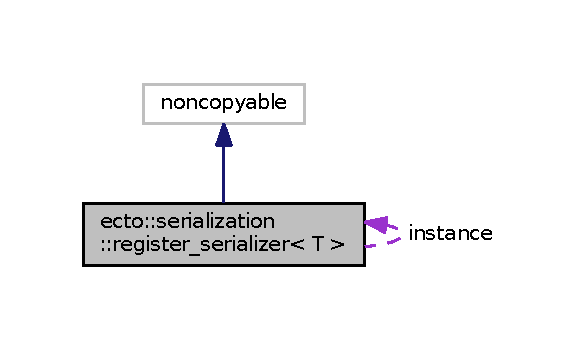
\includegraphics[width=350pt]{structecto_1_1serialization_1_1register__serializer__coll__graph}
\end{center}
\end{figure}
\subsection*{\-Public \-Types}
\begin{DoxyCompactItemize}
\item 
typedef \hyperlink{structecto_1_1serialization_1_1writer__}{writer\-\_\-}$<$ \-T, \*
boost\-::archive\-::binary\-\_\-oarchive $>$ \hyperlink{structecto_1_1serialization_1_1register__serializer_a31c9f04624076aa209e66232a511c627}{writer\-\_\-binary\-\_\-oa}
\item 
typedef \hyperlink{structecto_1_1serialization_1_1reader__}{reader\-\_\-}$<$ \-T, \*
boost\-::archive\-::binary\-\_\-iarchive $>$ \hyperlink{structecto_1_1serialization_1_1register__serializer_a7783674d19bdb5a7f2143953d6a7302f}{reader\-\_\-binary\-\_\-ia}
\end{DoxyCompactItemize}
\subsection*{\-Private \-Member \-Functions}
\begin{DoxyCompactItemize}
\item 
\hyperlink{structecto_1_1serialization_1_1register__serializer_ae339eb881e0afbb36bff03a34263c683}{register\-\_\-serializer} ()
\end{DoxyCompactItemize}
\subsection*{\-Static \-Private \-Attributes}
\begin{DoxyCompactItemize}
\item 
static const \hyperlink{structecto_1_1serialization_1_1register__serializer}{register\-\_\-serializer} \hyperlink{structecto_1_1serialization_1_1register__serializer_a742ed82697621237f599631009e47e05}{instance}
\end{DoxyCompactItemize}
\subsubsection*{template$<$typename T$>$ struct ecto\-::serialization\-::register\-\_\-serializer$<$ T $>$}



\subsection{\-Member \-Typedef \-Documentation}
\hypertarget{structecto_1_1serialization_1_1register__serializer_a7783674d19bdb5a7f2143953d6a7302f}{\index{ecto\-::serialization\-::register\-\_\-serializer@{ecto\-::serialization\-::register\-\_\-serializer}!reader\-\_\-binary\-\_\-ia@{reader\-\_\-binary\-\_\-ia}}
\index{reader\-\_\-binary\-\_\-ia@{reader\-\_\-binary\-\_\-ia}!ecto::serialization::register_serializer@{ecto\-::serialization\-::register\-\_\-serializer}}
\subsubsection[{reader\-\_\-binary\-\_\-ia}]{\setlength{\rightskip}{0pt plus 5cm}template$<$typename T $>$ typedef {\bf reader\-\_\-}$<$\-T, boost\-::archive\-::binary\-\_\-iarchive$>$ {\bf ecto\-::serialization\-::register\-\_\-serializer}$<$ \-T $>$\-::{\bf reader\-\_\-binary\-\_\-ia}}}\label{structecto_1_1serialization_1_1register__serializer_a7783674d19bdb5a7f2143953d6a7302f}
\hypertarget{structecto_1_1serialization_1_1register__serializer_a31c9f04624076aa209e66232a511c627}{\index{ecto\-::serialization\-::register\-\_\-serializer@{ecto\-::serialization\-::register\-\_\-serializer}!writer\-\_\-binary\-\_\-oa@{writer\-\_\-binary\-\_\-oa}}
\index{writer\-\_\-binary\-\_\-oa@{writer\-\_\-binary\-\_\-oa}!ecto::serialization::register_serializer@{ecto\-::serialization\-::register\-\_\-serializer}}
\subsubsection[{writer\-\_\-binary\-\_\-oa}]{\setlength{\rightskip}{0pt plus 5cm}template$<$typename T $>$ typedef {\bf writer\-\_\-}$<$\-T, boost\-::archive\-::binary\-\_\-oarchive$>$ {\bf ecto\-::serialization\-::register\-\_\-serializer}$<$ \-T $>$\-::{\bf writer\-\_\-binary\-\_\-oa}}}\label{structecto_1_1serialization_1_1register__serializer_a31c9f04624076aa209e66232a511c627}


\subsection{\-Constructor \& \-Destructor \-Documentation}
\hypertarget{structecto_1_1serialization_1_1register__serializer_ae339eb881e0afbb36bff03a34263c683}{\index{ecto\-::serialization\-::register\-\_\-serializer@{ecto\-::serialization\-::register\-\_\-serializer}!register\-\_\-serializer@{register\-\_\-serializer}}
\index{register\-\_\-serializer@{register\-\_\-serializer}!ecto::serialization::register_serializer@{ecto\-::serialization\-::register\-\_\-serializer}}
\subsubsection[{register\-\_\-serializer}]{\setlength{\rightskip}{0pt plus 5cm}template$<$typename T $>$ {\bf ecto\-::serialization\-::register\-\_\-serializer}$<$ \-T $>$\-::{\bf register\-\_\-serializer} (
\begin{DoxyParamCaption}
{}
\end{DoxyParamCaption}
)\hspace{0.3cm}{\ttfamily  \mbox{[}inline, private\mbox{]}}}}\label{structecto_1_1serialization_1_1register__serializer_ae339eb881e0afbb36bff03a34263c683}


\subsection{\-Member \-Data \-Documentation}
\hypertarget{structecto_1_1serialization_1_1register__serializer_a742ed82697621237f599631009e47e05}{\index{ecto\-::serialization\-::register\-\_\-serializer@{ecto\-::serialization\-::register\-\_\-serializer}!instance@{instance}}
\index{instance@{instance}!ecto::serialization::register_serializer@{ecto\-::serialization\-::register\-\_\-serializer}}
\subsubsection[{instance}]{\setlength{\rightskip}{0pt plus 5cm}template$<$typename T $>$ const {\bf register\-\_\-serializer}$<$ \-T $>$ {\bf ecto\-::serialization\-::register\-\_\-serializer}$<$ \-T $>$\-::{\bf instance}\hspace{0.3cm}{\ttfamily  \mbox{[}static, private\mbox{]}}}}\label{structecto_1_1serialization_1_1register__serializer_a742ed82697621237f599631009e47e05}


\-The documentation for this struct was generated from the following file\-:\begin{DoxyCompactItemize}
\item 
/home/vrabaud/workspace/recognition\-\_\-kitchen\-\_\-groovy/src/ecto/include/ecto/serialization/\hyperlink{serialization_2registry_8hpp}{registry.\-hpp}\end{DoxyCompactItemize}

\hypertarget{structecto_1_1registry_1_1registrator}{}\section{ecto\+:\+:registry\+:\+:registrator$<$ Module, T $>$ Struct Template Reference}
\label{structecto_1_1registry_1_1registrator}\index{ecto\+::registry\+::registrator$<$ Module, T $>$@{ecto\+::registry\+::registrator$<$ Module, T $>$}}


{\ttfamily \#include $<$registry.\+hpp$>$}



Collaboration diagram for ecto\+:\+:registry\+:\+:registrator$<$ Module, T $>$\+:\nopagebreak
\begin{figure}[H]
\begin{center}
\leavevmode
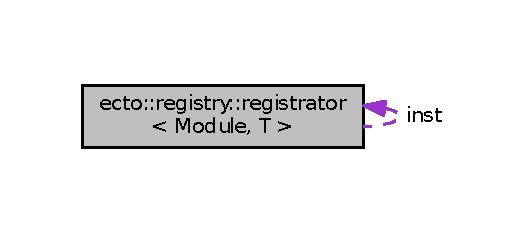
\includegraphics[width=254pt]{structecto_1_1registry_1_1registrator__coll__graph}
\end{center}
\end{figure}
\subsection*{Public Types}
\begin{DoxyCompactItemize}
\item 
typedef \+::\hyperlink{structecto_1_1cell__}{ecto\+::cell\+\_\+}$<$ T $>$ \hyperlink{structecto_1_1registry_1_1registrator_ae352ebfb18c87dc7fb3f649ecbe445fa}{cell\+\_\+t}
\end{DoxyCompactItemize}
\subsection*{Public Member Functions}
\begin{DoxyCompactItemize}
\item 
\hyperlink{structecto_1_1registry_1_1registrator_a3c8bafa2e65ef88c572c1779fb05fd12}{registrator} (const char $\ast$name, const char $\ast$docstring)
\item 
void \hyperlink{structecto_1_1registry_1_1registrator_a11572913b91238e8d6415bb89cc7ac1a}{operator()} () const 
\end{DoxyCompactItemize}
\subsection*{Static Public Member Functions}
\begin{DoxyCompactItemize}
\item 
static boost\+::shared\+\_\+ptr$<$ \hyperlink{structecto_1_1cell}{cell} $>$ \hyperlink{structecto_1_1registry_1_1registrator_aa46347f24e15fcc5955523d5e2adadf7}{create} ()
\end{DoxyCompactItemize}
\subsection*{Public Attributes}
\begin{DoxyCompactItemize}
\item 
const char $\ast$ \hyperlink{structecto_1_1registry_1_1registrator_a794acc964cefc0a374129823b4ee5246}{name\+\_\+}
\item 
const char $\ast$ \hyperlink{structecto_1_1registry_1_1registrator_a6eb361c892595a3d71ab627829c07bdb}{docstring\+\_\+}
\end{DoxyCompactItemize}
\subsection*{Static Public Attributes}
\begin{DoxyCompactItemize}
\item 
static const \hyperlink{structecto_1_1registry_1_1registrator}{registrator} \& \hyperlink{structecto_1_1registry_1_1registrator_a0b0f6e3aa1718476b962a007786e7496}{inst}
\end{DoxyCompactItemize}


\subsection{Member Typedef Documentation}
\hypertarget{structecto_1_1registry_1_1registrator_ae352ebfb18c87dc7fb3f649ecbe445fa}{}\index{ecto\+::registry\+::registrator@{ecto\+::registry\+::registrator}!cell\+\_\+t@{cell\+\_\+t}}
\index{cell\+\_\+t@{cell\+\_\+t}!ecto\+::registry\+::registrator@{ecto\+::registry\+::registrator}}
\subsubsection[{cell\+\_\+t}]{\setlength{\rightskip}{0pt plus 5cm}template$<$typename Module, typename T$>$ typedef \+::{\bf ecto\+::cell\+\_\+}$<$T$>$ {\bf ecto\+::registry\+::registrator}$<$ Module, T $>$\+::{\bf cell\+\_\+t}}\label{structecto_1_1registry_1_1registrator_ae352ebfb18c87dc7fb3f649ecbe445fa}


\subsection{Constructor \& Destructor Documentation}
\hypertarget{structecto_1_1registry_1_1registrator_a3c8bafa2e65ef88c572c1779fb05fd12}{}\index{ecto\+::registry\+::registrator@{ecto\+::registry\+::registrator}!registrator@{registrator}}
\index{registrator@{registrator}!ecto\+::registry\+::registrator@{ecto\+::registry\+::registrator}}
\subsubsection[{registrator}]{\setlength{\rightskip}{0pt plus 5cm}template$<$typename Module, typename T$>$ {\bf ecto\+::registry\+::registrator}$<$ Module, T $>$\+::{\bf registrator} (
\begin{DoxyParamCaption}
\item[{const char $\ast$}]{name, }
\item[{const char $\ast$}]{docstring}
\end{DoxyParamCaption}
)\hspace{0.3cm}{\ttfamily [inline]}, {\ttfamily [explicit]}}\label{structecto_1_1registry_1_1registrator_a3c8bafa2e65ef88c572c1779fb05fd12}


\subsection{Member Function Documentation}
\hypertarget{structecto_1_1registry_1_1registrator_aa46347f24e15fcc5955523d5e2adadf7}{}\index{ecto\+::registry\+::registrator@{ecto\+::registry\+::registrator}!create@{create}}
\index{create@{create}!ecto\+::registry\+::registrator@{ecto\+::registry\+::registrator}}
\subsubsection[{create}]{\setlength{\rightskip}{0pt plus 5cm}template$<$typename Module, typename T$>$ static boost\+::shared\+\_\+ptr$<${\bf cell}$>$ {\bf ecto\+::registry\+::registrator}$<$ Module, T $>$\+::create (
\begin{DoxyParamCaption}
{}
\end{DoxyParamCaption}
)\hspace{0.3cm}{\ttfamily [inline]}, {\ttfamily [static]}}\label{structecto_1_1registry_1_1registrator_aa46347f24e15fcc5955523d5e2adadf7}
\hypertarget{structecto_1_1registry_1_1registrator_a11572913b91238e8d6415bb89cc7ac1a}{}\index{ecto\+::registry\+::registrator@{ecto\+::registry\+::registrator}!operator()@{operator()}}
\index{operator()@{operator()}!ecto\+::registry\+::registrator@{ecto\+::registry\+::registrator}}
\subsubsection[{operator()}]{\setlength{\rightskip}{0pt plus 5cm}template$<$typename Module, typename T$>$ void {\bf ecto\+::registry\+::registrator}$<$ Module, T $>$\+::operator() (
\begin{DoxyParamCaption}
{}
\end{DoxyParamCaption}
) const\hspace{0.3cm}{\ttfamily [inline]}}\label{structecto_1_1registry_1_1registrator_a11572913b91238e8d6415bb89cc7ac1a}


\subsection{Member Data Documentation}
\hypertarget{structecto_1_1registry_1_1registrator_a6eb361c892595a3d71ab627829c07bdb}{}\index{ecto\+::registry\+::registrator@{ecto\+::registry\+::registrator}!docstring\+\_\+@{docstring\+\_\+}}
\index{docstring\+\_\+@{docstring\+\_\+}!ecto\+::registry\+::registrator@{ecto\+::registry\+::registrator}}
\subsubsection[{docstring\+\_\+}]{\setlength{\rightskip}{0pt plus 5cm}template$<$typename Module, typename T$>$ const char$\ast$ {\bf ecto\+::registry\+::registrator}$<$ Module, T $>$\+::docstring\+\_\+}\label{structecto_1_1registry_1_1registrator_a6eb361c892595a3d71ab627829c07bdb}
\hypertarget{structecto_1_1registry_1_1registrator_a0b0f6e3aa1718476b962a007786e7496}{}\index{ecto\+::registry\+::registrator@{ecto\+::registry\+::registrator}!inst@{inst}}
\index{inst@{inst}!ecto\+::registry\+::registrator@{ecto\+::registry\+::registrator}}
\subsubsection[{inst}]{\setlength{\rightskip}{0pt plus 5cm}template$<$typename Module, typename T$>$ const {\bf registrator}\& {\bf ecto\+::registry\+::registrator}$<$ Module, T $>$\+::inst\hspace{0.3cm}{\ttfamily [static]}}\label{structecto_1_1registry_1_1registrator_a0b0f6e3aa1718476b962a007786e7496}
\hypertarget{structecto_1_1registry_1_1registrator_a794acc964cefc0a374129823b4ee5246}{}\index{ecto\+::registry\+::registrator@{ecto\+::registry\+::registrator}!name\+\_\+@{name\+\_\+}}
\index{name\+\_\+@{name\+\_\+}!ecto\+::registry\+::registrator@{ecto\+::registry\+::registrator}}
\subsubsection[{name\+\_\+}]{\setlength{\rightskip}{0pt plus 5cm}template$<$typename Module, typename T$>$ const char$\ast$ {\bf ecto\+::registry\+::registrator}$<$ Module, T $>$\+::name\+\_\+}\label{structecto_1_1registry_1_1registrator_a794acc964cefc0a374129823b4ee5246}


The documentation for this struct was generated from the following file\+:\begin{DoxyCompactItemize}
\item 
/home/vrabaud/workspace/recognition\+\_\+kitchen/src/ecto/include/ecto/\hyperlink{registry_8hpp}{registry.\+hpp}\end{DoxyCompactItemize}

\hypertarget{structecto_1_1serialization_1_1registry}{}\section{ecto\+:\+:serialization\+:\+:registry$<$ Archive $>$ Struct Template Reference}
\label{structecto_1_1serialization_1_1registry}\index{ecto\+::serialization\+::registry$<$ Archive $>$@{ecto\+::serialization\+::registry$<$ Archive $>$}}


{\ttfamily \#include $<$registry.\+hpp$>$}



Inheritance diagram for ecto\+:\+:serialization\+:\+:registry$<$ Archive $>$\+:\nopagebreak
\begin{figure}[H]
\begin{center}
\leavevmode
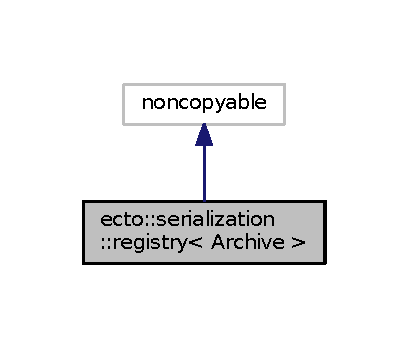
\includegraphics[width=196pt]{structecto_1_1serialization_1_1registry__inherit__graph}
\end{center}
\end{figure}


Collaboration diagram for ecto\+:\+:serialization\+:\+:registry$<$ Archive $>$\+:\nopagebreak
\begin{figure}[H]
\begin{center}
\leavevmode
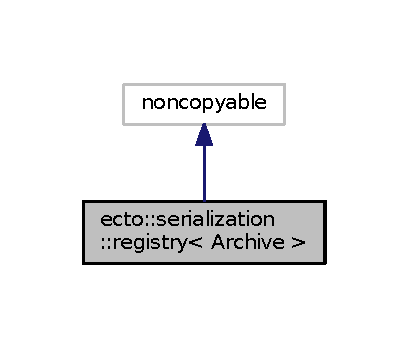
\includegraphics[width=196pt]{structecto_1_1serialization_1_1registry__coll__graph}
\end{center}
\end{figure}
\subsection*{Public Types}
\begin{DoxyCompactItemize}
\item 
typedef boost\+::function$<$ void(Archive \&, \hyperlink{classecto_1_1tendril}{tendril} \&)$>$ \hyperlink{structecto_1_1serialization_1_1registry_a9bbc5358e0b5bb519983c16db9c6391b}{serial\+\_\+fn\+\_\+t}
\item 
typedef std\+::map$<$ std\+::string, \hyperlink{structecto_1_1serialization_1_1registry_a9bbc5358e0b5bb519983c16db9c6391b}{serial\+\_\+fn\+\_\+t} $>$ \hyperlink{structecto_1_1serialization_1_1registry_a89253dc4749e297b132dacb9e14967c2}{serial\+\_\+map\+\_\+t}
\end{DoxyCompactItemize}
\subsection*{Public Member Functions}
\begin{DoxyCompactItemize}
\item 
{\footnotesize template$<$typename Serializer $>$ }\\void \hyperlink{structecto_1_1serialization_1_1registry_ae82f89f8e2bdcf2573671a6d390a94e2}{add} (const Serializer \&s)
\item 
void \hyperlink{structecto_1_1serialization_1_1registry_a9642b0813d8bb6c99dffb527b9d57419}{add} (const std\+::string \&name, \hyperlink{structecto_1_1serialization_1_1registry_a9bbc5358e0b5bb519983c16db9c6391b}{serial\+\_\+fn\+\_\+t} fnc)
\item 
void \hyperlink{structecto_1_1serialization_1_1registry_afaecca49afab42cb3f41a7a515b69cbb}{serialize} (const std\+::string \&key, Archive \&ar, \hyperlink{classecto_1_1tendril}{tendril} \&t) const 
\end{DoxyCompactItemize}
\subsection*{Static Public Member Functions}
\begin{DoxyCompactItemize}
\item 
static \hyperlink{structecto_1_1serialization_1_1registry}{registry}$<$ Archive $>$ \& \hyperlink{structecto_1_1serialization_1_1registry_a19aae99a3cc5ddb4b56d069faf01e300}{instance} ()
\end{DoxyCompactItemize}
\subsection*{Public Attributes}
\begin{DoxyCompactItemize}
\item 
\hyperlink{structecto_1_1serialization_1_1registry_a89253dc4749e297b132dacb9e14967c2}{serial\+\_\+map\+\_\+t} \hyperlink{structecto_1_1serialization_1_1registry_a7ef09466a24edc21695e3905c0a7921b}{serial\+\_\+map}
\end{DoxyCompactItemize}
\subsection*{Private Member Functions}
\begin{DoxyCompactItemize}
\item 
\hyperlink{structecto_1_1serialization_1_1registry_acbf5b14a8ef87e8a1324ad852e3e3f13}{registry} ()
\end{DoxyCompactItemize}


\subsection{Member Typedef Documentation}
\index{ecto\+::serialization\+::registry@{ecto\+::serialization\+::registry}!serial\+\_\+fn\+\_\+t@{serial\+\_\+fn\+\_\+t}}
\index{serial\+\_\+fn\+\_\+t@{serial\+\_\+fn\+\_\+t}!ecto\+::serialization\+::registry@{ecto\+::serialization\+::registry}}
\subsubsection[{\texorpdfstring{serial\+\_\+fn\+\_\+t}{serial_fn_t}}]{\setlength{\rightskip}{0pt plus 5cm}template$<$typename Archive$>$ typedef boost\+::function$<$void(Archive\&, {\bf tendril}\&)$>$ {\bf ecto\+::serialization\+::registry}$<$ Archive $>$\+::{\bf serial\+\_\+fn\+\_\+t}}\hypertarget{structecto_1_1serialization_1_1registry_a9bbc5358e0b5bb519983c16db9c6391b}{}\label{structecto_1_1serialization_1_1registry_a9bbc5358e0b5bb519983c16db9c6391b}
\index{ecto\+::serialization\+::registry@{ecto\+::serialization\+::registry}!serial\+\_\+map\+\_\+t@{serial\+\_\+map\+\_\+t}}
\index{serial\+\_\+map\+\_\+t@{serial\+\_\+map\+\_\+t}!ecto\+::serialization\+::registry@{ecto\+::serialization\+::registry}}
\subsubsection[{\texorpdfstring{serial\+\_\+map\+\_\+t}{serial_map_t}}]{\setlength{\rightskip}{0pt plus 5cm}template$<$typename Archive$>$ typedef std\+::map$<$std\+::string, {\bf serial\+\_\+fn\+\_\+t}$>$ {\bf ecto\+::serialization\+::registry}$<$ Archive $>$\+::{\bf serial\+\_\+map\+\_\+t}}\hypertarget{structecto_1_1serialization_1_1registry_a89253dc4749e297b132dacb9e14967c2}{}\label{structecto_1_1serialization_1_1registry_a89253dc4749e297b132dacb9e14967c2}


\subsection{Constructor \& Destructor Documentation}
\index{ecto\+::serialization\+::registry@{ecto\+::serialization\+::registry}!registry@{registry}}
\index{registry@{registry}!ecto\+::serialization\+::registry@{ecto\+::serialization\+::registry}}
\subsubsection[{\texorpdfstring{registry()}{registry()}}]{\setlength{\rightskip}{0pt plus 5cm}template$<$typename Archive$>$ {\bf ecto\+::serialization\+::registry}$<$ Archive $>$\+::{\bf registry} (
\begin{DoxyParamCaption}
{}
\end{DoxyParamCaption}
)\hspace{0.3cm}{\ttfamily [private]}}\hypertarget{structecto_1_1serialization_1_1registry_acbf5b14a8ef87e8a1324ad852e3e3f13}{}\label{structecto_1_1serialization_1_1registry_acbf5b14a8ef87e8a1324ad852e3e3f13}


\subsection{Member Function Documentation}
\index{ecto\+::serialization\+::registry@{ecto\+::serialization\+::registry}!add@{add}}
\index{add@{add}!ecto\+::serialization\+::registry@{ecto\+::serialization\+::registry}}
\subsubsection[{\texorpdfstring{add(const Serializer \&s)}{add(const Serializer &s)}}]{\setlength{\rightskip}{0pt plus 5cm}template$<$typename Archive$>$ template$<$typename Serializer $>$ void {\bf ecto\+::serialization\+::registry}$<$ Archive $>$\+::add (
\begin{DoxyParamCaption}
\item[{const Serializer \&}]{s}
\end{DoxyParamCaption}
)\hspace{0.3cm}{\ttfamily [inline]}}\hypertarget{structecto_1_1serialization_1_1registry_ae82f89f8e2bdcf2573671a6d390a94e2}{}\label{structecto_1_1serialization_1_1registry_ae82f89f8e2bdcf2573671a6d390a94e2}
\index{ecto\+::serialization\+::registry@{ecto\+::serialization\+::registry}!add@{add}}
\index{add@{add}!ecto\+::serialization\+::registry@{ecto\+::serialization\+::registry}}
\subsubsection[{\texorpdfstring{add(const std\+::string \&name, serial\+\_\+fn\+\_\+t fnc)}{add(const std::string &name, serial_fn_t fnc)}}]{\setlength{\rightskip}{0pt plus 5cm}template$<$typename Archive$>$ void {\bf ecto\+::serialization\+::registry}$<$ Archive $>$\+::add (
\begin{DoxyParamCaption}
\item[{const std\+::string \&}]{name, }
\item[{{\bf serial\+\_\+fn\+\_\+t}}]{fnc}
\end{DoxyParamCaption}
)}\hypertarget{structecto_1_1serialization_1_1registry_a9642b0813d8bb6c99dffb527b9d57419}{}\label{structecto_1_1serialization_1_1registry_a9642b0813d8bb6c99dffb527b9d57419}
\index{ecto\+::serialization\+::registry@{ecto\+::serialization\+::registry}!instance@{instance}}
\index{instance@{instance}!ecto\+::serialization\+::registry@{ecto\+::serialization\+::registry}}
\subsubsection[{\texorpdfstring{instance()}{instance()}}]{\setlength{\rightskip}{0pt plus 5cm}template$<$typename Archive$>$ static {\bf registry}$<$Archive$>$\& {\bf ecto\+::serialization\+::registry}$<$ Archive $>$\+::instance (
\begin{DoxyParamCaption}
{}
\end{DoxyParamCaption}
)\hspace{0.3cm}{\ttfamily [static]}}\hypertarget{structecto_1_1serialization_1_1registry_a19aae99a3cc5ddb4b56d069faf01e300}{}\label{structecto_1_1serialization_1_1registry_a19aae99a3cc5ddb4b56d069faf01e300}
\index{ecto\+::serialization\+::registry@{ecto\+::serialization\+::registry}!serialize@{serialize}}
\index{serialize@{serialize}!ecto\+::serialization\+::registry@{ecto\+::serialization\+::registry}}
\subsubsection[{\texorpdfstring{serialize(const std\+::string \&key, Archive \&ar, tendril \&t) const }{serialize(const std::string &key, Archive &ar, tendril &t) const }}]{\setlength{\rightskip}{0pt plus 5cm}template$<$typename Archive$>$ void {\bf ecto\+::serialization\+::registry}$<$ Archive $>$\+::serialize (
\begin{DoxyParamCaption}
\item[{const std\+::string \&}]{key, }
\item[{Archive \&}]{ar, }
\item[{{\bf tendril} \&}]{t}
\end{DoxyParamCaption}
) const}\hypertarget{structecto_1_1serialization_1_1registry_afaecca49afab42cb3f41a7a515b69cbb}{}\label{structecto_1_1serialization_1_1registry_afaecca49afab42cb3f41a7a515b69cbb}


\subsection{Member Data Documentation}
\index{ecto\+::serialization\+::registry@{ecto\+::serialization\+::registry}!serial\+\_\+map@{serial\+\_\+map}}
\index{serial\+\_\+map@{serial\+\_\+map}!ecto\+::serialization\+::registry@{ecto\+::serialization\+::registry}}
\subsubsection[{\texorpdfstring{serial\+\_\+map}{serial_map}}]{\setlength{\rightskip}{0pt plus 5cm}template$<$typename Archive$>$ {\bf serial\+\_\+map\+\_\+t} {\bf ecto\+::serialization\+::registry}$<$ Archive $>$\+::serial\+\_\+map}\hypertarget{structecto_1_1serialization_1_1registry_a7ef09466a24edc21695e3905c0a7921b}{}\label{structecto_1_1serialization_1_1registry_a7ef09466a24edc21695e3905c0a7921b}


The documentation for this struct was generated from the following file\+:\begin{DoxyCompactItemize}
\item 
/home/vrabaud/workspace/recognition\+\_\+kitchen/src/ecto/include/ecto/serialization/\hyperlink{serialization_2registry_8hpp}{registry.\+hpp}\end{DoxyCompactItemize}

\hypertarget{classecto_1_1scheduler}{}\section{ecto\+:\+:scheduler Class Reference}
\label{classecto_1_1scheduler}\index{ecto\+::scheduler@{ecto\+::scheduler}}


{\ttfamily \#include $<$scheduler.\+hpp$>$}



Collaboration diagram for ecto\+:\+:scheduler\+:\nopagebreak
\begin{figure}[H]
\begin{center}
\leavevmode
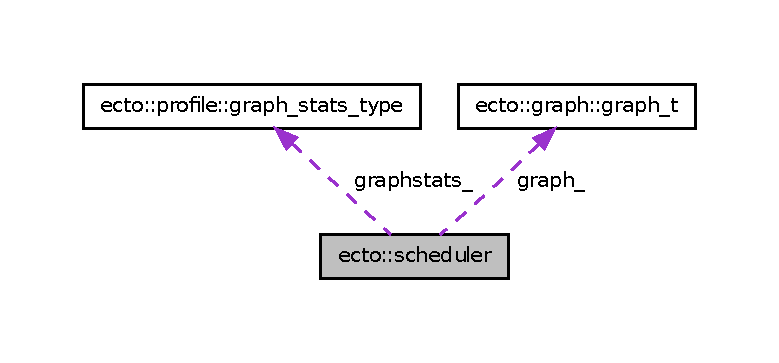
\includegraphics[width=350pt]{classecto_1_1scheduler__coll__graph}
\end{center}
\end{figure}
\subsection*{Public Types}
\begin{DoxyCompactItemize}
\item 
enum \hyperlink{classecto_1_1scheduler_a6b063d1c4bb9dad58d7ace61946b1200}{State} \{ \\*
\hyperlink{classecto_1_1scheduler_a6b063d1c4bb9dad58d7ace61946b1200a347092c6b9c4bbc7084bfa04d9ffb57f}{I\+N\+I\+T} = 0, 
\hyperlink{classecto_1_1scheduler_a6b063d1c4bb9dad58d7ace61946b1200aef190614c39d85b915b9ff2225eacf02}{R\+U\+N\+N\+I\+N\+G}, 
\hyperlink{classecto_1_1scheduler_a6b063d1c4bb9dad58d7ace61946b1200a3e140c949a41686e2e0481d13e89c010}{E\+X\+E\+C\+U\+T\+I\+N\+G}, 
\hyperlink{classecto_1_1scheduler_a6b063d1c4bb9dad58d7ace61946b1200a0cf2ac365020f8cd0a6860a3983a0dad}{S\+T\+O\+P\+P\+I\+N\+G}, 
\\*
\hyperlink{classecto_1_1scheduler_a6b063d1c4bb9dad58d7ace61946b1200aa9b97654759582b6e92fbc17a31623bd}{F\+I\+N\+I} = -\/1, 
\hyperlink{classecto_1_1scheduler_a6b063d1c4bb9dad58d7ace61946b1200a45aebc05bdc20659645ad6e1729db520}{E\+R\+R\+O\+R} = -\/2
 \}
\end{DoxyCompactItemize}
\subsection*{Public Member Functions}
\begin{DoxyCompactItemize}
\item 
\hyperlink{classecto_1_1scheduler_a3a2999bde52bfacfc194243ef2ae4f89}{scheduler} (\hyperlink{namespaceecto_a6b83be6cd685db71f03b14871653475f}{plasm\+\_\+ptr} p)
\item 
\hyperlink{classecto_1_1scheduler_aac758e34705ebab32cf66bdf42f0d89d}{$\sim$scheduler} ()
\item 
bool \hyperlink{classecto_1_1scheduler_ad917e3fa322f0a065e306afec7284d4e}{execute} (unsigned num\+\_\+iters=0)
\item 
bool \hyperlink{classecto_1_1scheduler_a6f723a36600b0a47c9b387c460cf3d59}{prepare\+\_\+jobs} (unsigned num\+\_\+iters=0)
\item 
bool \hyperlink{classecto_1_1scheduler_a7fcfe7583c13ff5d2294242aedfa0b1a}{run\+\_\+job} ()
\item 
bool \hyperlink{classecto_1_1scheduler_a326022cba6c3154f28f9694b7c9968fd}{run} (unsigned timeout\+\_\+usec)
\item 
bool \hyperlink{classecto_1_1scheduler_a8d5ce4f97e511341f315bb7621ba38f4}{run} ()
\item 
bool \hyperlink{classecto_1_1scheduler_a99ac4b8df3d015f6a39d0cf7607cc657}{running} () const 
\item 
bool \hyperlink{classecto_1_1scheduler_a13257817e1cc6c1ce04ef0bfdabc5375}{executing} () const 
\item 
void \hyperlink{classecto_1_1scheduler_ab974783264da5c33a19110926b5565f4}{stop} ()
\item 
std\+::string \hyperlink{classecto_1_1scheduler_a99d2f51779f856b3905bb8b493f091c4}{stats} () const 
\item 
\hyperlink{classecto_1_1scheduler_a6b063d1c4bb9dad58d7ace61946b1200}{State} \hyperlink{classecto_1_1scheduler_a5497ae108416ccdf7d80fa7c8e462992}{state} () const 
\end{DoxyCompactItemize}
\subsection*{Private Member Functions}
\begin{DoxyCompactItemize}
\item 
\hyperlink{classecto_1_1scheduler_a6b063d1c4bb9dad58d7ace61946b1200}{State} \hyperlink{classecto_1_1scheduler_a04cb7ea1040fcb02f5c843ca33ffa1a6}{state} (\hyperlink{classecto_1_1scheduler_a6b063d1c4bb9dad58d7ace61946b1200}{State})
\item 
void \hyperlink{classecto_1_1scheduler_adc21b65d6b046032648161c16ca89f77}{execute\+\_\+init} (unsigned num\+\_\+ite\+Rel\+With\+Deb\+Infors)
\item 
void \hyperlink{classecto_1_1scheduler_ae96db9aa735b4aec8eda6c1ea5616b95}{execute\+\_\+iter} (unsigned cur\+\_\+iter, unsigned num\+\_\+iters, std\+::size\+\_\+t stack\+\_\+idx)
\item 
void \hyperlink{classecto_1_1scheduler_abab4de26974143a076ac532ffac4f67f}{execute\+\_\+fini} ()
\item 
void \hyperlink{classecto_1_1scheduler_ae803a977a35883a6a0b8f83e7ba63d3c}{interrupt} ()
\item 
void \hyperlink{classecto_1_1scheduler_ad922a0a31e48a09ae6b6a95a4a1a20e5}{compute\+\_\+stack} ()
\end{DoxyCompactItemize}
\subsection*{Private Attributes}
\begin{DoxyCompactItemize}
\item 
\hyperlink{namespaceecto_a6b83be6cd685db71f03b14871653475f}{plasm\+\_\+ptr} \hyperlink{classecto_1_1scheduler_a9ccfb508a5bf75ec7ca69b475a7c7226}{plasm\+\_\+}
\item 
\hyperlink{structecto_1_1graph_1_1graph__t}{ecto\+::graph\+::graph\+\_\+t} \& \hyperlink{classecto_1_1scheduler_a79de9623f94d1003dc34f12fc69c5981}{graph\+\_\+}
\item 
std\+::vector$<$ ecto\+::graph\+::graph\+\_\+t\+::vertex\+\_\+descriptor $>$ \hyperlink{classecto_1_1scheduler_ad2b6561ebc08afd8cf8edaa39cb702b8}{stack\+\_\+}
\item 
\hyperlink{structecto_1_1profile_1_1graph__stats__type}{profile\+::graph\+\_\+stats\+\_\+type} \hyperlink{classecto_1_1scheduler_a6da29ce8fc4f4d2a1c451a577e049c62}{graphstats\+\_\+}
\item 
boost\+::asio\+::io\+\_\+service \hyperlink{classecto_1_1scheduler_af8f90a97a59811157c657cecb8512069}{io\+\_\+svc\+\_\+}
\item 
boost\+::mutex \hyperlink{classecto_1_1scheduler_a47a29f5a0e1f1ab8ce816b0c63442b5c}{mtx\+\_\+}
\item 
\hyperlink{classecto_1_1scheduler_a6b063d1c4bb9dad58d7ace61946b1200}{State} \hyperlink{classecto_1_1scheduler_a21d2aac4a8a2ef665942b7c9b741250c}{state\+\_\+}
\begin{DoxyCompactList}\small\item\em Current state of the scheduler. \end{DoxyCompactList}\item 
std\+::size\+\_\+t \hyperlink{classecto_1_1scheduler_a650d97445fe90ba4572d208430f71e20}{runners\+\_\+}
\begin{DoxyCompactList}\small\item\em Current number of \char`\"{}runners\char`\"{} (threads calling a run method). \end{DoxyCompactList}\item 
boost\+::signals2\+::connection \hyperlink{classecto_1_1scheduler_a7eedec3e00966ffa25a5172bdaa8b7c6}{interrupt\+\_\+connection}
\item 
bool \hyperlink{classecto_1_1scheduler_abbb89be5b75cc481087fc2b2b1f00147}{interrupted}
\end{DoxyCompactItemize}


\subsection{Detailed Description}
T\+O\+D\+O\+: Doc this class. T\+O\+D\+O\+: Need to share io\+\_\+svc\+\_\+ instances with other entities (schedulers+)? 

\subsection{Member Enumeration Documentation}
\hypertarget{classecto_1_1scheduler_a6b063d1c4bb9dad58d7ace61946b1200}{}\index{ecto\+::scheduler@{ecto\+::scheduler}!State@{State}}
\index{State@{State}!ecto\+::scheduler@{ecto\+::scheduler}}
\subsubsection[{State}]{\setlength{\rightskip}{0pt plus 5cm}enum {\bf ecto\+::scheduler\+::\+State}}\label{classecto_1_1scheduler_a6b063d1c4bb9dad58d7ace61946b1200}
Scheduler states. Values greater than 0 indicate a \char`\"{}running\char`\"{} state. \begin{Desc}
\item[Enumerator]\par
\begin{description}
\index{I\+N\+I\+T@{I\+N\+I\+T}!ecto\+::scheduler@{ecto\+::scheduler}}\index{ecto\+::scheduler@{ecto\+::scheduler}!I\+N\+I\+T@{I\+N\+I\+T}}\item[{\em 
\hypertarget{classecto_1_1scheduler_a6b063d1c4bb9dad58d7ace61946b1200a347092c6b9c4bbc7084bfa04d9ffb57f}{}I\+N\+I\+T\label{classecto_1_1scheduler_a6b063d1c4bb9dad58d7ace61946b1200a347092c6b9c4bbc7084bfa04d9ffb57f}
}]None of the execute$\ast$() methods have been called yet. \index{R\+U\+N\+N\+I\+N\+G@{R\+U\+N\+N\+I\+N\+G}!ecto\+::scheduler@{ecto\+::scheduler}}\index{ecto\+::scheduler@{ecto\+::scheduler}!R\+U\+N\+N\+I\+N\+G@{R\+U\+N\+N\+I\+N\+G}}\item[{\em 
\hypertarget{classecto_1_1scheduler_a6b063d1c4bb9dad58d7ace61946b1200aef190614c39d85b915b9ff2225eacf02}{}R\+U\+N\+N\+I\+N\+G\label{classecto_1_1scheduler_a6b063d1c4bb9dad58d7ace61946b1200aef190614c39d85b915b9ff2225eacf02}
}]One of the execute$\ast$() methods was called and successfully completed the specified number of iterations. \index{E\+X\+E\+C\+U\+T\+I\+N\+G@{E\+X\+E\+C\+U\+T\+I\+N\+G}!ecto\+::scheduler@{ecto\+::scheduler}}\index{ecto\+::scheduler@{ecto\+::scheduler}!E\+X\+E\+C\+U\+T\+I\+N\+G@{E\+X\+E\+C\+U\+T\+I\+N\+G}}\item[{\em 
\hypertarget{classecto_1_1scheduler_a6b063d1c4bb9dad58d7ace61946b1200a3e140c949a41686e2e0481d13e89c010}{}E\+X\+E\+C\+U\+T\+I\+N\+G\label{classecto_1_1scheduler_a6b063d1c4bb9dad58d7ace61946b1200a3e140c949a41686e2e0481d13e89c010}
}]\hyperlink{classecto_1_1scheduler_ad917e3fa322f0a065e306afec7284d4e}{execute()} is running, or jobs have been prepared and the specified number of iterations have not been completed. \index{S\+T\+O\+P\+P\+I\+N\+G@{S\+T\+O\+P\+P\+I\+N\+G}!ecto\+::scheduler@{ecto\+::scheduler}}\index{ecto\+::scheduler@{ecto\+::scheduler}!S\+T\+O\+P\+P\+I\+N\+G@{S\+T\+O\+P\+P\+I\+N\+G}}\item[{\em 
\hypertarget{classecto_1_1scheduler_a6b063d1c4bb9dad58d7ace61946b1200a0cf2ac365020f8cd0a6860a3983a0dad}{}S\+T\+O\+P\+P\+I\+N\+G\label{classecto_1_1scheduler_a6b063d1c4bb9dad58d7ace61946b1200a0cf2ac365020f8cd0a6860a3983a0dad}
}]\hyperlink{classecto_1_1scheduler_ab974783264da5c33a19110926b5565f4}{stop()} was called, but the scheduler has not stopped yet. \index{F\+I\+N\+I@{F\+I\+N\+I}!ecto\+::scheduler@{ecto\+::scheduler}}\index{ecto\+::scheduler@{ecto\+::scheduler}!F\+I\+N\+I@{F\+I\+N\+I}}\item[{\em 
\hypertarget{classecto_1_1scheduler_a6b063d1c4bb9dad58d7ace61946b1200aa9b97654759582b6e92fbc17a31623bd}{}F\+I\+N\+I\label{classecto_1_1scheduler_a6b063d1c4bb9dad58d7ace61946b1200aa9b97654759582b6e92fbc17a31623bd}
}]\hyperlink{classecto_1_1scheduler_ab974783264da5c33a19110926b5565f4}{stop()} completed, or one of the \hyperlink{structecto_1_1cell_a6b810671ee21f5dddbc1206abfb999f3}{cell\+::process()} calls returned \hyperlink{namespaceecto_a93d82cd28db695d53963fb696582762ca6803dad912ff60afb751d630ba35f0b3}{ecto\+::\+Q\+U\+I\+T} and the scheduler is no longer running. \index{E\+R\+R\+O\+R@{E\+R\+R\+O\+R}!ecto\+::scheduler@{ecto\+::scheduler}}\index{ecto\+::scheduler@{ecto\+::scheduler}!E\+R\+R\+O\+R@{E\+R\+R\+O\+R}}\item[{\em 
\hypertarget{classecto_1_1scheduler_a6b063d1c4bb9dad58d7ace61946b1200a45aebc05bdc20659645ad6e1729db520}{}E\+R\+R\+O\+R\label{classecto_1_1scheduler_a6b063d1c4bb9dad58d7ace61946b1200a45aebc05bdc20659645ad6e1729db520}
}]One of the \hyperlink{structecto_1_1cell_a6b810671ee21f5dddbc1206abfb999f3}{cell\+::process()} calls returned an error or threw, and the scheduler is no longer running. \end{description}
\end{Desc}


\subsection{Constructor \& Destructor Documentation}
\hypertarget{classecto_1_1scheduler_a3a2999bde52bfacfc194243ef2ae4f89}{}\index{ecto\+::scheduler@{ecto\+::scheduler}!scheduler@{scheduler}}
\index{scheduler@{scheduler}!ecto\+::scheduler@{ecto\+::scheduler}}
\subsubsection[{scheduler}]{\setlength{\rightskip}{0pt plus 5cm}ecto\+::scheduler\+::scheduler (
\begin{DoxyParamCaption}
\item[{{\bf plasm\+\_\+ptr}}]{p}
\end{DoxyParamCaption}
)\hspace{0.3cm}{\ttfamily [explicit]}}\label{classecto_1_1scheduler_a3a2999bde52bfacfc194243ef2ae4f89}
\hypertarget{classecto_1_1scheduler_aac758e34705ebab32cf66bdf42f0d89d}{}\index{ecto\+::scheduler@{ecto\+::scheduler}!````~scheduler@{$\sim$scheduler}}
\index{````~scheduler@{$\sim$scheduler}!ecto\+::scheduler@{ecto\+::scheduler}}
\subsubsection[{$\sim$scheduler}]{\setlength{\rightskip}{0pt plus 5cm}ecto\+::scheduler\+::$\sim$scheduler (
\begin{DoxyParamCaption}
{}
\end{DoxyParamCaption}
)}\label{classecto_1_1scheduler_aac758e34705ebab32cf66bdf42f0d89d}


\subsection{Member Function Documentation}
\hypertarget{classecto_1_1scheduler_ad922a0a31e48a09ae6b6a95a4a1a20e5}{}\index{ecto\+::scheduler@{ecto\+::scheduler}!compute\+\_\+stack@{compute\+\_\+stack}}
\index{compute\+\_\+stack@{compute\+\_\+stack}!ecto\+::scheduler@{ecto\+::scheduler}}
\subsubsection[{compute\+\_\+stack}]{\setlength{\rightskip}{0pt plus 5cm}void ecto\+::scheduler\+::compute\+\_\+stack (
\begin{DoxyParamCaption}
{}
\end{DoxyParamCaption}
)\hspace{0.3cm}{\ttfamily [private]}}\label{classecto_1_1scheduler_ad922a0a31e48a09ae6b6a95a4a1a20e5}
Check plasm for correctness, configure it, activate it, then sort it topologically to populate stack\+\_\+. This method is idempotent. \hypertarget{classecto_1_1scheduler_ad917e3fa322f0a065e306afec7284d4e}{}\index{ecto\+::scheduler@{ecto\+::scheduler}!execute@{execute}}
\index{execute@{execute}!ecto\+::scheduler@{ecto\+::scheduler}}
\subsubsection[{execute}]{\setlength{\rightskip}{0pt plus 5cm}bool ecto\+::scheduler\+::execute (
\begin{DoxyParamCaption}
\item[{unsigned}]{num\+\_\+iters = {\ttfamily 0}}
\end{DoxyParamCaption}
)}\label{classecto_1_1scheduler_ad917e3fa322f0a065e306afec7284d4e}
Synchronously execute plasm for num\+\_\+iters iterations. 
\begin{DoxyParams}[1]{Parameters}
\mbox{\tt in}  & {\em num\+\_\+iters} & The number of iterations to execute the plasm. 0 indicates that the plasm should be executed until some \hyperlink{structecto_1_1cell_a6b810671ee21f5dddbc1206abfb999f3}{cell\+::process()} call returns \hyperlink{namespaceecto_a93d82cd28db695d53963fb696582762ca6803dad912ff60afb751d630ba35f0b3}{ecto\+::\+Q\+U\+I\+T}. \\
\hline
\end{DoxyParams}
\begin{DoxyAttention}{Attention}
This call will block indefinately if num\+\_\+iters is 0. 
\end{DoxyAttention}
\hypertarget{classecto_1_1scheduler_abab4de26974143a076ac532ffac4f67f}{}\index{ecto\+::scheduler@{ecto\+::scheduler}!execute\+\_\+fini@{execute\+\_\+fini}}
\index{execute\+\_\+fini@{execute\+\_\+fini}!ecto\+::scheduler@{ecto\+::scheduler}}
\subsubsection[{execute\+\_\+fini}]{\setlength{\rightskip}{0pt plus 5cm}void ecto\+::scheduler\+::execute\+\_\+fini (
\begin{DoxyParamCaption}
{}
\end{DoxyParamCaption}
)\hspace{0.3cm}{\ttfamily [private]}}\label{classecto_1_1scheduler_abab4de26974143a076ac532ffac4f67f}
\hypertarget{classecto_1_1scheduler_adc21b65d6b046032648161c16ca89f77}{}\index{ecto\+::scheduler@{ecto\+::scheduler}!execute\+\_\+init@{execute\+\_\+init}}
\index{execute\+\_\+init@{execute\+\_\+init}!ecto\+::scheduler@{ecto\+::scheduler}}
\subsubsection[{execute\+\_\+init}]{\setlength{\rightskip}{0pt plus 5cm}void ecto\+::scheduler\+::execute\+\_\+init (
\begin{DoxyParamCaption}
\item[{unsigned}]{num\+\_\+ite\+Rel\+With\+Deb\+Infors}
\end{DoxyParamCaption}
)\hspace{0.3cm}{\ttfamily [private]}}\label{classecto_1_1scheduler_adc21b65d6b046032648161c16ca89f77}
\hypertarget{classecto_1_1scheduler_ae96db9aa735b4aec8eda6c1ea5616b95}{}\index{ecto\+::scheduler@{ecto\+::scheduler}!execute\+\_\+iter@{execute\+\_\+iter}}
\index{execute\+\_\+iter@{execute\+\_\+iter}!ecto\+::scheduler@{ecto\+::scheduler}}
\subsubsection[{execute\+\_\+iter}]{\setlength{\rightskip}{0pt plus 5cm}void ecto\+::scheduler\+::execute\+\_\+iter (
\begin{DoxyParamCaption}
\item[{unsigned}]{cur\+\_\+iter, }
\item[{unsigned}]{num\+\_\+iters, }
\item[{std\+::size\+\_\+t}]{stack\+\_\+idx}
\end{DoxyParamCaption}
)\hspace{0.3cm}{\ttfamily [private]}}\label{classecto_1_1scheduler_ae96db9aa735b4aec8eda6c1ea5616b95}
\hypertarget{classecto_1_1scheduler_a13257817e1cc6c1ce04ef0bfdabc5375}{}\index{ecto\+::scheduler@{ecto\+::scheduler}!executing@{executing}}
\index{executing@{executing}!ecto\+::scheduler@{ecto\+::scheduler}}
\subsubsection[{executing}]{\setlength{\rightskip}{0pt plus 5cm}bool ecto\+::scheduler\+::executing (
\begin{DoxyParamCaption}
{}
\end{DoxyParamCaption}
) const\hspace{0.3cm}{\ttfamily [inline]}}\label{classecto_1_1scheduler_a13257817e1cc6c1ce04ef0bfdabc5375}
\begin{DoxyReturn}{Returns}
true indicates that the plasm is currently in an executing state ( state\+\_\+ == E\+X\+E\+C\+U\+T\+I\+N\+G). 
\end{DoxyReturn}
\hypertarget{classecto_1_1scheduler_ae803a977a35883a6a0b8f83e7ba63d3c}{}\index{ecto\+::scheduler@{ecto\+::scheduler}!interrupt@{interrupt}}
\index{interrupt@{interrupt}!ecto\+::scheduler@{ecto\+::scheduler}}
\subsubsection[{interrupt}]{\setlength{\rightskip}{0pt plus 5cm}void ecto\+::scheduler\+::interrupt (
\begin{DoxyParamCaption}
{}
\end{DoxyParamCaption}
)\hspace{0.3cm}{\ttfamily [private]}}\label{classecto_1_1scheduler_ae803a977a35883a6a0b8f83e7ba63d3c}
\hypertarget{classecto_1_1scheduler_a6f723a36600b0a47c9b387c460cf3d59}{}\index{ecto\+::scheduler@{ecto\+::scheduler}!prepare\+\_\+jobs@{prepare\+\_\+jobs}}
\index{prepare\+\_\+jobs@{prepare\+\_\+jobs}!ecto\+::scheduler@{ecto\+::scheduler}}
\subsubsection[{prepare\+\_\+jobs}]{\setlength{\rightskip}{0pt plus 5cm}bool ecto\+::scheduler\+::prepare\+\_\+jobs (
\begin{DoxyParamCaption}
\item[{unsigned}]{num\+\_\+iters = {\ttfamily 0}}
\end{DoxyParamCaption}
)}\label{classecto_1_1scheduler_a6f723a36600b0a47c9b387c460cf3d59}
Prepare jobs for execution of a plasm over num\+\_\+iters iterations. No actual work will be done without calling the run$\ast$() methods. This just fills up the io service queues with the jobs required for initialisation and execution of the plasm over the specified number of iterations. 
\begin{DoxyParams}[1]{Parameters}
\mbox{\tt in}  & {\em num\+\_\+iters} & The number of iterations to execute the plasm. 0 indicates that the plasm should be executed until some \hyperlink{structecto_1_1cell_a6b810671ee21f5dddbc1206abfb999f3}{cell\+::process()} call returns \hyperlink{namespaceecto_a93d82cd28db695d53963fb696582762ca6803dad912ff60afb751d630ba35f0b3}{ecto\+::\+Q\+U\+I\+T}. \\
\hline
\end{DoxyParams}
\begin{DoxyAttention}{Attention}
A call to \hyperlink{classecto_1_1scheduler_a8d5ce4f97e511341f315bb7621ba38f4}{run()} will block indefinately if num\+\_\+iters is 0. 
\end{DoxyAttention}
\hypertarget{classecto_1_1scheduler_a326022cba6c3154f28f9694b7c9968fd}{}\index{ecto\+::scheduler@{ecto\+::scheduler}!run@{run}}
\index{run@{run}!ecto\+::scheduler@{ecto\+::scheduler}}
\subsubsection[{run}]{\setlength{\rightskip}{0pt plus 5cm}bool ecto\+::scheduler\+::run (
\begin{DoxyParamCaption}
\item[{unsigned}]{timeout\+\_\+usec}
\end{DoxyParamCaption}
)}\label{classecto_1_1scheduler_a326022cba6c3154f28f9694b7c9968fd}
Run jobs in the calling thread for the specified number of microseconds, or until the io\+\_\+service is depleted. 
\begin{DoxyParams}[1]{Parameters}
\mbox{\tt in}  & {\em timeout\+\_\+usec} & The number of microsecs to run io\+\_\+service jobs. \\
\hline
\end{DoxyParams}
\begin{DoxyAttention}{Attention}
Assuming the io\+\_\+service does not run out of work, this is the minimum amount of time that will be spent running jobs. 
\end{DoxyAttention}
\begin{DoxyReturn}{Returns}
true indicates that the scheduler is still \char`\"{}running.\char`\"{} 
\end{DoxyReturn}
\hypertarget{classecto_1_1scheduler_a8d5ce4f97e511341f315bb7621ba38f4}{}\index{ecto\+::scheduler@{ecto\+::scheduler}!run@{run}}
\index{run@{run}!ecto\+::scheduler@{ecto\+::scheduler}}
\subsubsection[{run}]{\setlength{\rightskip}{0pt plus 5cm}bool ecto\+::scheduler\+::run (
\begin{DoxyParamCaption}
{}
\end{DoxyParamCaption}
)}\label{classecto_1_1scheduler_a8d5ce4f97e511341f315bb7621ba38f4}
Run jobs in the calling thread until the io\+\_\+service is depleted. \begin{DoxyReturn}{Returns}
true indicates that the scheduler is still \char`\"{}running.\char`\"{} 
\end{DoxyReturn}
\hypertarget{classecto_1_1scheduler_a7fcfe7583c13ff5d2294242aedfa0b1a}{}\index{ecto\+::scheduler@{ecto\+::scheduler}!run\+\_\+job@{run\+\_\+job}}
\index{run\+\_\+job@{run\+\_\+job}!ecto\+::scheduler@{ecto\+::scheduler}}
\subsubsection[{run\+\_\+job}]{\setlength{\rightskip}{0pt plus 5cm}bool ecto\+::scheduler\+::run\+\_\+job (
\begin{DoxyParamCaption}
{}
\end{DoxyParamCaption}
)}\label{classecto_1_1scheduler_a7fcfe7583c13ff5d2294242aedfa0b1a}
Run one job in the calling thread of execution. \begin{DoxyNote}{Note}
A job is not necessarily (but is usually) a \hyperlink{structecto_1_1cell_a6b810671ee21f5dddbc1206abfb999f3}{cell\+::process()} call. 
\end{DoxyNote}
\begin{DoxyAttention}{Attention}
If using python cells, this method must be called from the main python thread. 
\end{DoxyAttention}
\begin{DoxyReturn}{Returns}
true indicates that the scheduler is still \char`\"{}running.\char`\"{} 
\end{DoxyReturn}
\hypertarget{classecto_1_1scheduler_a99ac4b8df3d015f6a39d0cf7607cc657}{}\index{ecto\+::scheduler@{ecto\+::scheduler}!running@{running}}
\index{running@{running}!ecto\+::scheduler@{ecto\+::scheduler}}
\subsubsection[{running}]{\setlength{\rightskip}{0pt plus 5cm}bool ecto\+::scheduler\+::running (
\begin{DoxyParamCaption}
{}
\end{DoxyParamCaption}
) const\hspace{0.3cm}{\ttfamily [inline]}}\label{classecto_1_1scheduler_a99ac4b8df3d015f6a39d0cf7607cc657}
\begin{DoxyReturn}{Returns}
true indicates that the plasm is currently in a running state (state\+\_\+ $>$ 0, i.\+e. R\+U\+N\+N\+I\+N\+G, E\+X\+E\+C\+U\+T\+I\+N\+G, or S\+T\+O\+P\+P\+I\+N\+G). 
\end{DoxyReturn}
\hypertarget{classecto_1_1scheduler_a5497ae108416ccdf7d80fa7c8e462992}{}\index{ecto\+::scheduler@{ecto\+::scheduler}!state@{state}}
\index{state@{state}!ecto\+::scheduler@{ecto\+::scheduler}}
\subsubsection[{state}]{\setlength{\rightskip}{0pt plus 5cm}{\bf scheduler\+::\+State} ecto\+::scheduler\+::state (
\begin{DoxyParamCaption}
{}
\end{DoxyParamCaption}
) const\hspace{0.3cm}{\ttfamily [inline]}}\label{classecto_1_1scheduler_a5497ae108416ccdf7d80fa7c8e462992}
\begin{DoxyReturn}{Returns}
The current scheduler state. 
\end{DoxyReturn}
\hypertarget{classecto_1_1scheduler_a04cb7ea1040fcb02f5c843ca33ffa1a6}{}\index{ecto\+::scheduler@{ecto\+::scheduler}!state@{state}}
\index{state@{state}!ecto\+::scheduler@{ecto\+::scheduler}}
\subsubsection[{state}]{\setlength{\rightskip}{0pt plus 5cm}{\bf scheduler\+::\+State} ecto\+::scheduler\+::state (
\begin{DoxyParamCaption}
\item[{{\bf State}}]{state}
\end{DoxyParamCaption}
)\hspace{0.3cm}{\ttfamily [inline]}, {\ttfamily [private]}}\label{classecto_1_1scheduler_a04cb7ea1040fcb02f5c843ca33ffa1a6}
\hypertarget{classecto_1_1scheduler_a99d2f51779f856b3905bb8b493f091c4}{}\index{ecto\+::scheduler@{ecto\+::scheduler}!stats@{stats}}
\index{stats@{stats}!ecto\+::scheduler@{ecto\+::scheduler}}
\subsubsection[{stats}]{\setlength{\rightskip}{0pt plus 5cm}std\+::string ecto\+::scheduler\+::stats (
\begin{DoxyParamCaption}
{}
\end{DoxyParamCaption}
) const\hspace{0.3cm}{\ttfamily [inline]}}\label{classecto_1_1scheduler_a99d2f51779f856b3905bb8b493f091c4}
\begin{DoxyReturn}{Returns}
The current graph execution stats. 
\end{DoxyReturn}
\hypertarget{classecto_1_1scheduler_ab974783264da5c33a19110926b5565f4}{}\index{ecto\+::scheduler@{ecto\+::scheduler}!stop@{stop}}
\index{stop@{stop}!ecto\+::scheduler@{ecto\+::scheduler}}
\subsubsection[{stop}]{\setlength{\rightskip}{0pt plus 5cm}void ecto\+::scheduler\+::stop (
\begin{DoxyParamCaption}
{}
\end{DoxyParamCaption}
)}\label{classecto_1_1scheduler_ab974783264da5c33a19110926b5565f4}
Stop the scheduler, and flush any jobs in the io\+\_\+service. \begin{DoxyNote}{Note}
The scheduler will no longer be in the running state. 
\end{DoxyNote}
\begin{DoxyAttention}{Attention}
The plasm may be in the middle of the stack when it is stopped, but successive calls to execute$\ast$() start from the beginning. 
\end{DoxyAttention}


\subsection{Member Data Documentation}
\hypertarget{classecto_1_1scheduler_a79de9623f94d1003dc34f12fc69c5981}{}\index{ecto\+::scheduler@{ecto\+::scheduler}!graph\+\_\+@{graph\+\_\+}}
\index{graph\+\_\+@{graph\+\_\+}!ecto\+::scheduler@{ecto\+::scheduler}}
\subsubsection[{graph\+\_\+}]{\setlength{\rightskip}{0pt plus 5cm}{\bf ecto\+::graph\+::graph\+\_\+t}\& ecto\+::scheduler\+::graph\+\_\+\hspace{0.3cm}{\ttfamily [private]}}\label{classecto_1_1scheduler_a79de9623f94d1003dc34f12fc69c5981}
\hypertarget{classecto_1_1scheduler_a6da29ce8fc4f4d2a1c451a577e049c62}{}\index{ecto\+::scheduler@{ecto\+::scheduler}!graphstats\+\_\+@{graphstats\+\_\+}}
\index{graphstats\+\_\+@{graphstats\+\_\+}!ecto\+::scheduler@{ecto\+::scheduler}}
\subsubsection[{graphstats\+\_\+}]{\setlength{\rightskip}{0pt plus 5cm}{\bf profile\+::graph\+\_\+stats\+\_\+type} ecto\+::scheduler\+::graphstats\+\_\+\hspace{0.3cm}{\ttfamily [private]}}\label{classecto_1_1scheduler_a6da29ce8fc4f4d2a1c451a577e049c62}
\hypertarget{classecto_1_1scheduler_a7eedec3e00966ffa25a5172bdaa8b7c6}{}\index{ecto\+::scheduler@{ecto\+::scheduler}!interrupt\+\_\+connection@{interrupt\+\_\+connection}}
\index{interrupt\+\_\+connection@{interrupt\+\_\+connection}!ecto\+::scheduler@{ecto\+::scheduler}}
\subsubsection[{interrupt\+\_\+connection}]{\setlength{\rightskip}{0pt plus 5cm}boost\+::signals2\+::connection ecto\+::scheduler\+::interrupt\+\_\+connection\hspace{0.3cm}{\ttfamily [private]}}\label{classecto_1_1scheduler_a7eedec3e00966ffa25a5172bdaa8b7c6}
\hypertarget{classecto_1_1scheduler_abbb89be5b75cc481087fc2b2b1f00147}{}\index{ecto\+::scheduler@{ecto\+::scheduler}!interrupted@{interrupted}}
\index{interrupted@{interrupted}!ecto\+::scheduler@{ecto\+::scheduler}}
\subsubsection[{interrupted}]{\setlength{\rightskip}{0pt plus 5cm}bool ecto\+::scheduler\+::interrupted\hspace{0.3cm}{\ttfamily [private]}}\label{classecto_1_1scheduler_abbb89be5b75cc481087fc2b2b1f00147}
\hypertarget{classecto_1_1scheduler_af8f90a97a59811157c657cecb8512069}{}\index{ecto\+::scheduler@{ecto\+::scheduler}!io\+\_\+svc\+\_\+@{io\+\_\+svc\+\_\+}}
\index{io\+\_\+svc\+\_\+@{io\+\_\+svc\+\_\+}!ecto\+::scheduler@{ecto\+::scheduler}}
\subsubsection[{io\+\_\+svc\+\_\+}]{\setlength{\rightskip}{0pt plus 5cm}boost\+::asio\+::io\+\_\+service ecto\+::scheduler\+::io\+\_\+svc\+\_\+\hspace{0.3cm}{\ttfamily [private]}}\label{classecto_1_1scheduler_af8f90a97a59811157c657cecb8512069}
\hypertarget{classecto_1_1scheduler_a47a29f5a0e1f1ab8ce816b0c63442b5c}{}\index{ecto\+::scheduler@{ecto\+::scheduler}!mtx\+\_\+@{mtx\+\_\+}}
\index{mtx\+\_\+@{mtx\+\_\+}!ecto\+::scheduler@{ecto\+::scheduler}}
\subsubsection[{mtx\+\_\+}]{\setlength{\rightskip}{0pt plus 5cm}boost\+::mutex ecto\+::scheduler\+::mtx\+\_\+\hspace{0.3cm}{\ttfamily [mutable]}, {\ttfamily [private]}}\label{classecto_1_1scheduler_a47a29f5a0e1f1ab8ce816b0c63442b5c}
\hypertarget{classecto_1_1scheduler_a9ccfb508a5bf75ec7ca69b475a7c7226}{}\index{ecto\+::scheduler@{ecto\+::scheduler}!plasm\+\_\+@{plasm\+\_\+}}
\index{plasm\+\_\+@{plasm\+\_\+}!ecto\+::scheduler@{ecto\+::scheduler}}
\subsubsection[{plasm\+\_\+}]{\setlength{\rightskip}{0pt plus 5cm}{\bf plasm\+\_\+ptr} ecto\+::scheduler\+::plasm\+\_\+\hspace{0.3cm}{\ttfamily [private]}}\label{classecto_1_1scheduler_a9ccfb508a5bf75ec7ca69b475a7c7226}
\hypertarget{classecto_1_1scheduler_a650d97445fe90ba4572d208430f71e20}{}\index{ecto\+::scheduler@{ecto\+::scheduler}!runners\+\_\+@{runners\+\_\+}}
\index{runners\+\_\+@{runners\+\_\+}!ecto\+::scheduler@{ecto\+::scheduler}}
\subsubsection[{runners\+\_\+}]{\setlength{\rightskip}{0pt plus 5cm}std\+::size\+\_\+t ecto\+::scheduler\+::runners\+\_\+\hspace{0.3cm}{\ttfamily [private]}}\label{classecto_1_1scheduler_a650d97445fe90ba4572d208430f71e20}


Current number of \char`\"{}runners\char`\"{} (threads calling a run method). 

\hypertarget{classecto_1_1scheduler_ad2b6561ebc08afd8cf8edaa39cb702b8}{}\index{ecto\+::scheduler@{ecto\+::scheduler}!stack\+\_\+@{stack\+\_\+}}
\index{stack\+\_\+@{stack\+\_\+}!ecto\+::scheduler@{ecto\+::scheduler}}
\subsubsection[{stack\+\_\+}]{\setlength{\rightskip}{0pt plus 5cm}std\+::vector$<$ecto\+::graph\+::graph\+\_\+t\+::vertex\+\_\+descriptor$>$ ecto\+::scheduler\+::stack\+\_\+\hspace{0.3cm}{\ttfamily [private]}}\label{classecto_1_1scheduler_ad2b6561ebc08afd8cf8edaa39cb702b8}
\hypertarget{classecto_1_1scheduler_a21d2aac4a8a2ef665942b7c9b741250c}{}\index{ecto\+::scheduler@{ecto\+::scheduler}!state\+\_\+@{state\+\_\+}}
\index{state\+\_\+@{state\+\_\+}!ecto\+::scheduler@{ecto\+::scheduler}}
\subsubsection[{state\+\_\+}]{\setlength{\rightskip}{0pt plus 5cm}{\bf State} ecto\+::scheduler\+::state\+\_\+\hspace{0.3cm}{\ttfamily [private]}}\label{classecto_1_1scheduler_a21d2aac4a8a2ef665942b7c9b741250c}


Current state of the scheduler. 



The documentation for this class was generated from the following file\+:\begin{DoxyCompactItemize}
\item 
/home/vrabaud/workspace/recognition\+\_\+kitchen/src/ecto/include/ecto/\hyperlink{scheduler_8hpp}{scheduler.\+hpp}\end{DoxyCompactItemize}

\hypertarget{classecto_1_1py_1_1scoped__call__back__to__python}{\section{ecto\-:\-:py\-:\-:scoped\-\_\-call\-\_\-back\-\_\-to\-\_\-python \-Class \-Reference}
\label{classecto_1_1py_1_1scoped__call__back__to__python}\index{ecto\-::py\-::scoped\-\_\-call\-\_\-back\-\_\-to\-\_\-python@{ecto\-::py\-::scoped\-\_\-call\-\_\-back\-\_\-to\-\_\-python}}
}


{\ttfamily \#include $<$python.\-hpp$>$}



\-Collaboration diagram for ecto\-:\-:py\-:\-:scoped\-\_\-call\-\_\-back\-\_\-to\-\_\-python\-:\nopagebreak
\begin{figure}[H]
\begin{center}
\leavevmode
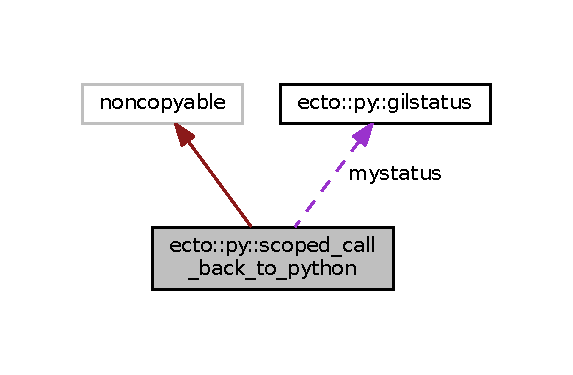
\includegraphics[width=276pt]{classecto_1_1py_1_1scoped__call__back__to__python__coll__graph}
\end{center}
\end{figure}
\subsection*{\-Public \-Member \-Functions}
\begin{DoxyCompactItemize}
\item 
\hyperlink{classecto_1_1py_1_1scoped__call__back__to__python_aa0e62dcba9ee21268b612d0a70849b2d}{scoped\-\_\-call\-\_\-back\-\_\-to\-\_\-python} (const char $\ast$file, unsigned line)
\item 
\hyperlink{classecto_1_1py_1_1scoped__call__back__to__python_a55b49e169de3007a19bb3881d96c38cc}{$\sim$scoped\-\_\-call\-\_\-back\-\_\-to\-\_\-python} ()
\end{DoxyCompactItemize}
\subsection*{\-Private \-Attributes}
\begin{DoxyCompactItemize}
\item 
\-Py\-G\-I\-L\-State\-\_\-\-S\-T\-A\-T\-E \hyperlink{classecto_1_1py_1_1scoped__call__back__to__python_a67de9bb9e263a7e77cefe47e75b18512}{gilstate}
\item 
bool \hyperlink{classecto_1_1py_1_1scoped__call__back__to__python_a4f4d2f01e986f7b93028996a7bd8498f}{have}
\item 
\hyperlink{structecto_1_1py_1_1gilstatus}{gilstatus} \hyperlink{classecto_1_1py_1_1scoped__call__back__to__python_a421a7edb2c8c08321c015312217caad7}{mystatus}
\end{DoxyCompactItemize}


\subsection{\-Constructor \& \-Destructor \-Documentation}
\hypertarget{classecto_1_1py_1_1scoped__call__back__to__python_aa0e62dcba9ee21268b612d0a70849b2d}{\index{ecto\-::py\-::scoped\-\_\-call\-\_\-back\-\_\-to\-\_\-python@{ecto\-::py\-::scoped\-\_\-call\-\_\-back\-\_\-to\-\_\-python}!scoped\-\_\-call\-\_\-back\-\_\-to\-\_\-python@{scoped\-\_\-call\-\_\-back\-\_\-to\-\_\-python}}
\index{scoped\-\_\-call\-\_\-back\-\_\-to\-\_\-python@{scoped\-\_\-call\-\_\-back\-\_\-to\-\_\-python}!ecto::py::scoped_call_back_to_python@{ecto\-::py\-::scoped\-\_\-call\-\_\-back\-\_\-to\-\_\-python}}
\subsubsection[{scoped\-\_\-call\-\_\-back\-\_\-to\-\_\-python}]{\setlength{\rightskip}{0pt plus 5cm}{\bf ecto\-::py\-::scoped\-\_\-call\-\_\-back\-\_\-to\-\_\-python\-::scoped\-\_\-call\-\_\-back\-\_\-to\-\_\-python} (
\begin{DoxyParamCaption}
\item[{const char $\ast$}]{file, }
\item[{unsigned}]{line}
\end{DoxyParamCaption}
)}}\label{classecto_1_1py_1_1scoped__call__back__to__python_aa0e62dcba9ee21268b612d0a70849b2d}
\hypertarget{classecto_1_1py_1_1scoped__call__back__to__python_a55b49e169de3007a19bb3881d96c38cc}{\index{ecto\-::py\-::scoped\-\_\-call\-\_\-back\-\_\-to\-\_\-python@{ecto\-::py\-::scoped\-\_\-call\-\_\-back\-\_\-to\-\_\-python}!$\sim$scoped\-\_\-call\-\_\-back\-\_\-to\-\_\-python@{$\sim$scoped\-\_\-call\-\_\-back\-\_\-to\-\_\-python}}
\index{$\sim$scoped\-\_\-call\-\_\-back\-\_\-to\-\_\-python@{$\sim$scoped\-\_\-call\-\_\-back\-\_\-to\-\_\-python}!ecto::py::scoped_call_back_to_python@{ecto\-::py\-::scoped\-\_\-call\-\_\-back\-\_\-to\-\_\-python}}
\subsubsection[{$\sim$scoped\-\_\-call\-\_\-back\-\_\-to\-\_\-python}]{\setlength{\rightskip}{0pt plus 5cm}{\bf ecto\-::py\-::scoped\-\_\-call\-\_\-back\-\_\-to\-\_\-python\-::$\sim$scoped\-\_\-call\-\_\-back\-\_\-to\-\_\-python} (
\begin{DoxyParamCaption}
{}
\end{DoxyParamCaption}
)}}\label{classecto_1_1py_1_1scoped__call__back__to__python_a55b49e169de3007a19bb3881d96c38cc}


\subsection{\-Member \-Data \-Documentation}
\hypertarget{classecto_1_1py_1_1scoped__call__back__to__python_a67de9bb9e263a7e77cefe47e75b18512}{\index{ecto\-::py\-::scoped\-\_\-call\-\_\-back\-\_\-to\-\_\-python@{ecto\-::py\-::scoped\-\_\-call\-\_\-back\-\_\-to\-\_\-python}!gilstate@{gilstate}}
\index{gilstate@{gilstate}!ecto::py::scoped_call_back_to_python@{ecto\-::py\-::scoped\-\_\-call\-\_\-back\-\_\-to\-\_\-python}}
\subsubsection[{gilstate}]{\setlength{\rightskip}{0pt plus 5cm}\-Py\-G\-I\-L\-State\-\_\-\-S\-T\-A\-T\-E {\bf ecto\-::py\-::scoped\-\_\-call\-\_\-back\-\_\-to\-\_\-python\-::gilstate}\hspace{0.3cm}{\ttfamily  \mbox{[}private\mbox{]}}}}\label{classecto_1_1py_1_1scoped__call__back__to__python_a67de9bb9e263a7e77cefe47e75b18512}
\hypertarget{classecto_1_1py_1_1scoped__call__back__to__python_a4f4d2f01e986f7b93028996a7bd8498f}{\index{ecto\-::py\-::scoped\-\_\-call\-\_\-back\-\_\-to\-\_\-python@{ecto\-::py\-::scoped\-\_\-call\-\_\-back\-\_\-to\-\_\-python}!have@{have}}
\index{have@{have}!ecto::py::scoped_call_back_to_python@{ecto\-::py\-::scoped\-\_\-call\-\_\-back\-\_\-to\-\_\-python}}
\subsubsection[{have}]{\setlength{\rightskip}{0pt plus 5cm}bool {\bf ecto\-::py\-::scoped\-\_\-call\-\_\-back\-\_\-to\-\_\-python\-::have}\hspace{0.3cm}{\ttfamily  \mbox{[}private\mbox{]}}}}\label{classecto_1_1py_1_1scoped__call__back__to__python_a4f4d2f01e986f7b93028996a7bd8498f}
\hypertarget{classecto_1_1py_1_1scoped__call__back__to__python_a421a7edb2c8c08321c015312217caad7}{\index{ecto\-::py\-::scoped\-\_\-call\-\_\-back\-\_\-to\-\_\-python@{ecto\-::py\-::scoped\-\_\-call\-\_\-back\-\_\-to\-\_\-python}!mystatus@{mystatus}}
\index{mystatus@{mystatus}!ecto::py::scoped_call_back_to_python@{ecto\-::py\-::scoped\-\_\-call\-\_\-back\-\_\-to\-\_\-python}}
\subsubsection[{mystatus}]{\setlength{\rightskip}{0pt plus 5cm}{\bf gilstatus} {\bf ecto\-::py\-::scoped\-\_\-call\-\_\-back\-\_\-to\-\_\-python\-::mystatus}\hspace{0.3cm}{\ttfamily  \mbox{[}private\mbox{]}}}}\label{classecto_1_1py_1_1scoped__call__back__to__python_a421a7edb2c8c08321c015312217caad7}


\-The documentation for this class was generated from the following file\-:\begin{DoxyCompactItemize}
\item 
/home/vrabaud/workspace/recognition\-\_\-kitchen\-\_\-groovy/src/ecto/include/ecto/\hyperlink{python_8hpp}{python.\-hpp}\end{DoxyCompactItemize}

\hypertarget{classecto_1_1py_1_1scoped__gil__release}{}\section{ecto\+:\+:py\+:\+:scoped\+\_\+gil\+\_\+release Class Reference}
\label{classecto_1_1py_1_1scoped__gil__release}\index{ecto\+::py\+::scoped\+\_\+gil\+\_\+release@{ecto\+::py\+::scoped\+\_\+gil\+\_\+release}}


{\ttfamily \#include $<$python.\+hpp$>$}



Inheritance diagram for ecto\+:\+:py\+:\+:scoped\+\_\+gil\+\_\+release\+:\nopagebreak
\begin{figure}[H]
\begin{center}
\leavevmode
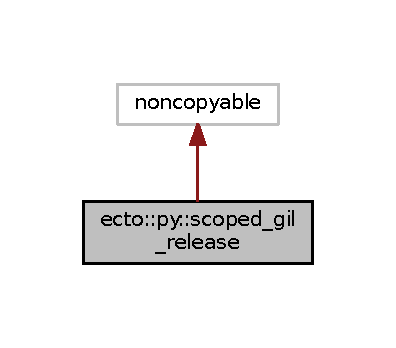
\includegraphics[width=190pt]{classecto_1_1py_1_1scoped__gil__release__inherit__graph}
\end{center}
\end{figure}


Collaboration diagram for ecto\+:\+:py\+:\+:scoped\+\_\+gil\+\_\+release\+:\nopagebreak
\begin{figure}[H]
\begin{center}
\leavevmode
\includegraphics[width=276pt]{classecto_1_1py_1_1scoped__gil__release__coll__graph}
\end{center}
\end{figure}
\subsection*{Public Member Functions}
\begin{DoxyCompactItemize}
\item 
\hyperlink{classecto_1_1py_1_1scoped__gil__release_afd4cb62267206421eca93969a8bb0865}{scoped\+\_\+gil\+\_\+release} (const char $\ast$file, unsigned line)
\item 
\hyperlink{classecto_1_1py_1_1scoped__gil__release_addd644daf557129d6584829cda6b9cc0}{$\sim$scoped\+\_\+gil\+\_\+release} ()
\end{DoxyCompactItemize}
\subsection*{Private Attributes}
\begin{DoxyCompactItemize}
\item 
bool \hyperlink{classecto_1_1py_1_1scoped__gil__release_a9e9fbf0c5819ac1b706437d99a6459a3}{mine}
\item 
\hyperlink{structecto_1_1py_1_1gilstatus}{gilstatus} \hyperlink{classecto_1_1py_1_1scoped__gil__release_a888a6813c86b9bbd2d5cd0d4a0f7e2f2}{mystatus}
\end{DoxyCompactItemize}
\subsection*{Static Private Attributes}
\begin{DoxyCompactItemize}
\item 
static std\+::map$<$ boost\+::thread\+::id, Py\+Thread\+State $\ast$ $>$ \hyperlink{classecto_1_1py_1_1scoped__gil__release_a5ecad50e9899f01f3779ac22009af5a4}{thread\+\_\+states}
\end{DoxyCompactItemize}


\subsection{Constructor \& Destructor Documentation}
\hypertarget{classecto_1_1py_1_1scoped__gil__release_afd4cb62267206421eca93969a8bb0865}{}\index{ecto\+::py\+::scoped\+\_\+gil\+\_\+release@{ecto\+::py\+::scoped\+\_\+gil\+\_\+release}!scoped\+\_\+gil\+\_\+release@{scoped\+\_\+gil\+\_\+release}}
\index{scoped\+\_\+gil\+\_\+release@{scoped\+\_\+gil\+\_\+release}!ecto\+::py\+::scoped\+\_\+gil\+\_\+release@{ecto\+::py\+::scoped\+\_\+gil\+\_\+release}}
\subsubsection[{scoped\+\_\+gil\+\_\+release}]{\setlength{\rightskip}{0pt plus 5cm}ecto\+::py\+::scoped\+\_\+gil\+\_\+release\+::scoped\+\_\+gil\+\_\+release (
\begin{DoxyParamCaption}
\item[{const char $\ast$}]{file, }
\item[{unsigned}]{line}
\end{DoxyParamCaption}
)}\label{classecto_1_1py_1_1scoped__gil__release_afd4cb62267206421eca93969a8bb0865}
\hypertarget{classecto_1_1py_1_1scoped__gil__release_addd644daf557129d6584829cda6b9cc0}{}\index{ecto\+::py\+::scoped\+\_\+gil\+\_\+release@{ecto\+::py\+::scoped\+\_\+gil\+\_\+release}!````~scoped\+\_\+gil\+\_\+release@{$\sim$scoped\+\_\+gil\+\_\+release}}
\index{````~scoped\+\_\+gil\+\_\+release@{$\sim$scoped\+\_\+gil\+\_\+release}!ecto\+::py\+::scoped\+\_\+gil\+\_\+release@{ecto\+::py\+::scoped\+\_\+gil\+\_\+release}}
\subsubsection[{$\sim$scoped\+\_\+gil\+\_\+release}]{\setlength{\rightskip}{0pt plus 5cm}ecto\+::py\+::scoped\+\_\+gil\+\_\+release\+::$\sim$scoped\+\_\+gil\+\_\+release (
\begin{DoxyParamCaption}
{}
\end{DoxyParamCaption}
)}\label{classecto_1_1py_1_1scoped__gil__release_addd644daf557129d6584829cda6b9cc0}


\subsection{Member Data Documentation}
\hypertarget{classecto_1_1py_1_1scoped__gil__release_a9e9fbf0c5819ac1b706437d99a6459a3}{}\index{ecto\+::py\+::scoped\+\_\+gil\+\_\+release@{ecto\+::py\+::scoped\+\_\+gil\+\_\+release}!mine@{mine}}
\index{mine@{mine}!ecto\+::py\+::scoped\+\_\+gil\+\_\+release@{ecto\+::py\+::scoped\+\_\+gil\+\_\+release}}
\subsubsection[{mine}]{\setlength{\rightskip}{0pt plus 5cm}bool ecto\+::py\+::scoped\+\_\+gil\+\_\+release\+::mine\hspace{0.3cm}{\ttfamily [private]}}\label{classecto_1_1py_1_1scoped__gil__release_a9e9fbf0c5819ac1b706437d99a6459a3}
\hypertarget{classecto_1_1py_1_1scoped__gil__release_a888a6813c86b9bbd2d5cd0d4a0f7e2f2}{}\index{ecto\+::py\+::scoped\+\_\+gil\+\_\+release@{ecto\+::py\+::scoped\+\_\+gil\+\_\+release}!mystatus@{mystatus}}
\index{mystatus@{mystatus}!ecto\+::py\+::scoped\+\_\+gil\+\_\+release@{ecto\+::py\+::scoped\+\_\+gil\+\_\+release}}
\subsubsection[{mystatus}]{\setlength{\rightskip}{0pt plus 5cm}{\bf gilstatus} ecto\+::py\+::scoped\+\_\+gil\+\_\+release\+::mystatus\hspace{0.3cm}{\ttfamily [private]}}\label{classecto_1_1py_1_1scoped__gil__release_a888a6813c86b9bbd2d5cd0d4a0f7e2f2}
\hypertarget{classecto_1_1py_1_1scoped__gil__release_a5ecad50e9899f01f3779ac22009af5a4}{}\index{ecto\+::py\+::scoped\+\_\+gil\+\_\+release@{ecto\+::py\+::scoped\+\_\+gil\+\_\+release}!thread\+\_\+states@{thread\+\_\+states}}
\index{thread\+\_\+states@{thread\+\_\+states}!ecto\+::py\+::scoped\+\_\+gil\+\_\+release@{ecto\+::py\+::scoped\+\_\+gil\+\_\+release}}
\subsubsection[{thread\+\_\+states}]{\setlength{\rightskip}{0pt plus 5cm}std\+::map$<$boost\+::thread\+::id, Py\+Thread\+State$\ast$$>$ ecto\+::py\+::scoped\+\_\+gil\+\_\+release\+::thread\+\_\+states\hspace{0.3cm}{\ttfamily [static]}, {\ttfamily [private]}}\label{classecto_1_1py_1_1scoped__gil__release_a5ecad50e9899f01f3779ac22009af5a4}


The documentation for this class was generated from the following file\+:\begin{DoxyCompactItemize}
\item 
/home/vrabaud/workspace/recognition\+\_\+kitchen/src/ecto/include/ecto/\hyperlink{python_8hpp}{python.\+hpp}\end{DoxyCompactItemize}

\hypertarget{classecto_1_1atomic_1_1scoped__lock}{\section{ecto\-:\-:atomic$<$ \-T $>$\-:\-:scoped\-\_\-lock \-Class \-Reference}
\label{classecto_1_1atomic_1_1scoped__lock}\index{ecto\-::atomic$<$ T $>$\-::scoped\-\_\-lock@{ecto\-::atomic$<$ T $>$\-::scoped\-\_\-lock}}
}


{\ttfamily \#include $<$atomic.\-hpp$>$}

\subsection*{\-Public \-Member \-Functions}
\begin{DoxyCompactItemize}
\item 
\hyperlink{classecto_1_1atomic_1_1scoped__lock_aa5a512f623ed5bd0f4010e200ad86e14}{scoped\-\_\-lock} (\hyperlink{classecto_1_1atomic}{atomic} \&a\-\_\-)
\end{DoxyCompactItemize}
\subsection*{\-Public \-Attributes}
\begin{DoxyCompactItemize}
\item 
\-T \& \hyperlink{classecto_1_1atomic_1_1scoped__lock_a89aa811b27815c91f99b3673a7f76753}{value}
\end{DoxyCompactItemize}
\subsection*{\-Private \-Attributes}
\begin{DoxyCompactItemize}
\item 
boost\-::mutex\-::scoped\-\_\-lock \hyperlink{classecto_1_1atomic_1_1scoped__lock_a637b9c7c8246e2ac352cb03fa9f4b229}{sl}
\end{DoxyCompactItemize}
\subsubsection*{template$<$typename T$>$ class ecto\-::atomic$<$ T $>$\-::scoped\-\_\-lock}



\subsection{\-Constructor \& \-Destructor \-Documentation}
\hypertarget{classecto_1_1atomic_1_1scoped__lock_aa5a512f623ed5bd0f4010e200ad86e14}{\index{ecto\-::atomic\-::scoped\-\_\-lock@{ecto\-::atomic\-::scoped\-\_\-lock}!scoped\-\_\-lock@{scoped\-\_\-lock}}
\index{scoped\-\_\-lock@{scoped\-\_\-lock}!ecto::atomic::scoped_lock@{ecto\-::atomic\-::scoped\-\_\-lock}}
\subsubsection[{scoped\-\_\-lock}]{\setlength{\rightskip}{0pt plus 5cm}template$<$typename T $>$ {\bf ecto\-::atomic}$<$ \-T $>$\-::{\bf scoped\-\_\-lock\-::scoped\-\_\-lock} (
\begin{DoxyParamCaption}
\item[{{\bf atomic} \&}]{a\-\_\-}
\end{DoxyParamCaption}
)\hspace{0.3cm}{\ttfamily  \mbox{[}inline\mbox{]}}}}\label{classecto_1_1atomic_1_1scoped__lock_aa5a512f623ed5bd0f4010e200ad86e14}


\subsection{\-Member \-Data \-Documentation}
\hypertarget{classecto_1_1atomic_1_1scoped__lock_a637b9c7c8246e2ac352cb03fa9f4b229}{\index{ecto\-::atomic\-::scoped\-\_\-lock@{ecto\-::atomic\-::scoped\-\_\-lock}!sl@{sl}}
\index{sl@{sl}!ecto::atomic::scoped_lock@{ecto\-::atomic\-::scoped\-\_\-lock}}
\subsubsection[{sl}]{\setlength{\rightskip}{0pt plus 5cm}template$<$typename T $>$ boost\-::mutex\-::scoped\-\_\-lock {\bf ecto\-::atomic}$<$ \-T $>$\-::{\bf scoped\-\_\-lock\-::sl}\hspace{0.3cm}{\ttfamily  \mbox{[}private\mbox{]}}}}\label{classecto_1_1atomic_1_1scoped__lock_a637b9c7c8246e2ac352cb03fa9f4b229}
\hypertarget{classecto_1_1atomic_1_1scoped__lock_a89aa811b27815c91f99b3673a7f76753}{\index{ecto\-::atomic\-::scoped\-\_\-lock@{ecto\-::atomic\-::scoped\-\_\-lock}!value@{value}}
\index{value@{value}!ecto::atomic::scoped_lock@{ecto\-::atomic\-::scoped\-\_\-lock}}
\subsubsection[{value}]{\setlength{\rightskip}{0pt plus 5cm}template$<$typename T $>$ \-T\& {\bf ecto\-::atomic}$<$ \-T $>$\-::{\bf scoped\-\_\-lock\-::value}}}\label{classecto_1_1atomic_1_1scoped__lock_a89aa811b27815c91f99b3673a7f76753}


\-The documentation for this class was generated from the following file\-:\begin{DoxyCompactItemize}
\item 
/home/vrabaud/workspace/recognition\-\_\-kitchen\-\_\-groovy/src/ecto/include/ecto/\hyperlink{atomic_8hpp}{atomic.\-hpp}\end{DoxyCompactItemize}

\hypertarget{structecto_1_1spore}{}\section{ecto\+:\+:spore$<$ T $>$ Class Template Reference}
\label{structecto_1_1spore}\index{ecto\+::spore$<$ T $>$@{ecto\+::spore$<$ T $>$}}


The spore is a typed handle for tendrils, making holding onto tendrils a bit easier.  




{\ttfamily \#include $<$spore.\+hpp$>$}

\subsection*{Public Types}
\begin{DoxyCompactItemize}
\item 
typedef \hyperlink{structecto_1_1spore}{spore}$<$ T $>$ \hyperlink{structecto_1_1spore_aa1e4c8dec72f4671c3469b84136677e4}{this\+\_\+type}
\item 
typedef T \hyperlink{structecto_1_1spore_af36d72731a0e1b823de1b411c34b1a1c}{value\+\_\+type}
\item 
typedef T \& \hyperlink{structecto_1_1spore_a79afa6b324736afc257bc89c6c770f81}{reference\+\_\+type}
\item 
typedef T $\ast$ \hyperlink{structecto_1_1spore_af00c161eec3285210e59c856aff26456}{pointer\+\_\+type}
\item 
typedef const T $\ast$ \hyperlink{structecto_1_1spore_af1219cc7b5343824699fc7f66a5c5891}{const\+\_\+pointer\+\_\+type}
\item 
typedef \hyperlink{namespaceecto_a84fb5f6130275382e5cbeb5fdececa78}{tendril\+\_\+ptr} this\+\_\+type\+::$\ast$ \hyperlink{structecto_1_1spore_a162474193fb3865f81f8b49b74858aa3}{unspecified\+\_\+bool\+\_\+type}
\end{DoxyCompactItemize}
\subsection*{Public Member Functions}
\begin{DoxyCompactItemize}
\item 
\hyperlink{structecto_1_1spore_a6b22569e73747f63644005c77d0fccd8}{spore} ()
\item 
\hyperlink{structecto_1_1spore_af45353900f648ef26ff9eb778dd61f23}{spore} (\hyperlink{namespaceecto_a84fb5f6130275382e5cbeb5fdececa78}{tendril\+\_\+ptr} t)
\item 
\hyperlink{structecto_1_1spore}{spore}$<$ T $>$ \& \hyperlink{structecto_1_1spore_ac46e4114f6e01b3acfa4a7ae4dd9dc67}{set\+\_\+callback} (typename boost\+::function1$<$ void, T $>$ cb)
\item 
\hyperlink{structecto_1_1spore}{spore}$<$ T $>$ \& \hyperlink{structecto_1_1spore_a979e896020612cd69604f8dad43f412d}{notify} ()
\item 
\hyperlink{structecto_1_1spore}{spore}$<$ T $>$ \& \hyperlink{structecto_1_1spore_a5eb3c4df0a6b798de09a76e2efbb5fb0}{set\+\_\+doc} (const std\+::string \&doc)
\item 
\hyperlink{structecto_1_1spore}{spore}$<$ T $>$ \& \hyperlink{structecto_1_1spore_a1d4ad4266f0e03bcf5b3c930cb9428a9}{set\+\_\+default\+\_\+val} (const T \&val)
\item 
bool \hyperlink{structecto_1_1spore_a3a358fb5a6cf0d18c854399285e98184}{dirty} () const 
\item 
void \hyperlink{structecto_1_1spore_a82d0d47b28034003965e8f70f4afea59}{dirty} (bool d)
\item 
bool \hyperlink{structecto_1_1spore_ae982e7c491c3445a6b4672494c6151b7}{user\+\_\+supplied} () const 
\item 
bool \hyperlink{structecto_1_1spore_a6c1f818917367c7c1e04e2d362257317}{has\+\_\+default} () const 
\item 
\hyperlink{structecto_1_1spore}{spore}$<$ T $>$ \& \hyperlink{structecto_1_1spore_a94342d6ff2601ae701dc4b66e53cb05c}{required} (bool b)
\item 
bool \hyperlink{structecto_1_1spore_a3520306f4699901fe09cd0fe0cd29ab0}{required} () const 
\item 
\hyperlink{structecto_1_1spore_af00c161eec3285210e59c856aff26456}{pointer\+\_\+type} \hyperlink{structecto_1_1spore_ad84fe1edeea4944545266bdf3b93556b}{operator-\/$>$} ()
\item 
\hyperlink{structecto_1_1spore_af1219cc7b5343824699fc7f66a5c5891}{const\+\_\+pointer\+\_\+type} \hyperlink{structecto_1_1spore_aeab6c0fdaf10bf4a3d1570d3eef46bd1}{operator-\/$>$} () const 
\item 
\hyperlink{structecto_1_1spore_a79afa6b324736afc257bc89c6c770f81}{reference\+\_\+type} \hyperlink{structecto_1_1spore_a6d693f3096c3fede0c85351d36adaded}{operator$\ast$} ()
\item 
\hyperlink{structecto_1_1spore_af1219cc7b5343824699fc7f66a5c5891}{const\+\_\+pointer\+\_\+type} \hyperlink{structecto_1_1spore_ae13ad63a891e8ed71d9010c18b754588}{operator$\ast$} () const 
\item 
\hyperlink{structecto_1_1spore_ae47aff3850e59591aed5fe2ad0b8d567}{operator unspecified\+\_\+bool\+\_\+type} () const 
\end{DoxyCompactItemize}
\subsection*{Private Member Functions}
\begin{DoxyCompactItemize}
\item 
\hyperlink{namespaceecto_a84fb5f6130275382e5cbeb5fdececa78}{tendril\+\_\+ptr} \hyperlink{structecto_1_1spore_a42f435f8c44fea74854382e0526e36ca}{get} ()
\item 
\hyperlink{namespaceecto_ad01f26ee47597f71a6f86ee34bb3ffe4}{tendril\+\_\+cptr} \hyperlink{structecto_1_1spore_a07c4091d4e5c14c30de319ec0f14b7de}{get} () const 
\end{DoxyCompactItemize}
\subsection*{Private Attributes}
\begin{DoxyCompactItemize}
\item 
\hyperlink{namespaceecto_a84fb5f6130275382e5cbeb5fdececa78}{tendril\+\_\+ptr} \hyperlink{structecto_1_1spore_a17e2ffe6861f828cad58904d20f117d4}{tendril\+\_\+}
\end{DoxyCompactItemize}


\subsection{Detailed Description}
\subsubsection*{template$<$typename T$>$\\*
class ecto\+::spore$<$ T $>$}

The spore is a typed handle for tendrils, making holding onto tendrils a bit easier. 

\subsection{Member Typedef Documentation}
\index{ecto\+::spore@{ecto\+::spore}!const\+\_\+pointer\+\_\+type@{const\+\_\+pointer\+\_\+type}}
\index{const\+\_\+pointer\+\_\+type@{const\+\_\+pointer\+\_\+type}!ecto\+::spore@{ecto\+::spore}}
\subsubsection[{\texorpdfstring{const\+\_\+pointer\+\_\+type}{const_pointer_type}}]{\setlength{\rightskip}{0pt plus 5cm}template$<$typename T$>$ typedef const T$\ast$ {\bf ecto\+::spore}$<$ T $>$\+::{\bf const\+\_\+pointer\+\_\+type}}\hypertarget{structecto_1_1spore_af1219cc7b5343824699fc7f66a5c5891}{}\label{structecto_1_1spore_af1219cc7b5343824699fc7f66a5c5891}
\index{ecto\+::spore@{ecto\+::spore}!pointer\+\_\+type@{pointer\+\_\+type}}
\index{pointer\+\_\+type@{pointer\+\_\+type}!ecto\+::spore@{ecto\+::spore}}
\subsubsection[{\texorpdfstring{pointer\+\_\+type}{pointer_type}}]{\setlength{\rightskip}{0pt plus 5cm}template$<$typename T$>$ typedef T$\ast$ {\bf ecto\+::spore}$<$ T $>$\+::{\bf pointer\+\_\+type}}\hypertarget{structecto_1_1spore_af00c161eec3285210e59c856aff26456}{}\label{structecto_1_1spore_af00c161eec3285210e59c856aff26456}
\index{ecto\+::spore@{ecto\+::spore}!reference\+\_\+type@{reference\+\_\+type}}
\index{reference\+\_\+type@{reference\+\_\+type}!ecto\+::spore@{ecto\+::spore}}
\subsubsection[{\texorpdfstring{reference\+\_\+type}{reference_type}}]{\setlength{\rightskip}{0pt plus 5cm}template$<$typename T$>$ typedef T\& {\bf ecto\+::spore}$<$ T $>$\+::{\bf reference\+\_\+type}}\hypertarget{structecto_1_1spore_a79afa6b324736afc257bc89c6c770f81}{}\label{structecto_1_1spore_a79afa6b324736afc257bc89c6c770f81}
\index{ecto\+::spore@{ecto\+::spore}!this\+\_\+type@{this\+\_\+type}}
\index{this\+\_\+type@{this\+\_\+type}!ecto\+::spore@{ecto\+::spore}}
\subsubsection[{\texorpdfstring{this\+\_\+type}{this_type}}]{\setlength{\rightskip}{0pt plus 5cm}template$<$typename T$>$ typedef {\bf spore}$<$T$>$ {\bf ecto\+::spore}$<$ T $>$\+::{\bf this\+\_\+type}}\hypertarget{structecto_1_1spore_aa1e4c8dec72f4671c3469b84136677e4}{}\label{structecto_1_1spore_aa1e4c8dec72f4671c3469b84136677e4}
\index{ecto\+::spore@{ecto\+::spore}!unspecified\+\_\+bool\+\_\+type@{unspecified\+\_\+bool\+\_\+type}}
\index{unspecified\+\_\+bool\+\_\+type@{unspecified\+\_\+bool\+\_\+type}!ecto\+::spore@{ecto\+::spore}}
\subsubsection[{\texorpdfstring{unspecified\+\_\+bool\+\_\+type}{unspecified_bool_type}}]{\setlength{\rightskip}{0pt plus 5cm}template$<$typename T$>$ typedef {\bf tendril\+\_\+ptr} this\+\_\+type\+::$\ast$ {\bf ecto\+::spore}$<$ T $>$\+::{\bf unspecified\+\_\+bool\+\_\+type}}\hypertarget{structecto_1_1spore_a162474193fb3865f81f8b49b74858aa3}{}\label{structecto_1_1spore_a162474193fb3865f81f8b49b74858aa3}
\index{ecto\+::spore@{ecto\+::spore}!value\+\_\+type@{value\+\_\+type}}
\index{value\+\_\+type@{value\+\_\+type}!ecto\+::spore@{ecto\+::spore}}
\subsubsection[{\texorpdfstring{value\+\_\+type}{value_type}}]{\setlength{\rightskip}{0pt plus 5cm}template$<$typename T$>$ typedef T {\bf ecto\+::spore}$<$ T $>$\+::{\bf value\+\_\+type}}\hypertarget{structecto_1_1spore_af36d72731a0e1b823de1b411c34b1a1c}{}\label{structecto_1_1spore_af36d72731a0e1b823de1b411c34b1a1c}


\subsection{Constructor \& Destructor Documentation}
\index{ecto\+::spore@{ecto\+::spore}!spore@{spore}}
\index{spore@{spore}!ecto\+::spore@{ecto\+::spore}}
\subsubsection[{\texorpdfstring{spore()}{spore()}}]{\setlength{\rightskip}{0pt plus 5cm}template$<$typename T$>$ {\bf ecto\+::spore}$<$ T $>$\+::{\bf spore} (
\begin{DoxyParamCaption}
{}
\end{DoxyParamCaption}
)\hspace{0.3cm}{\ttfamily [inline]}}\hypertarget{structecto_1_1spore_a6b22569e73747f63644005c77d0fccd8}{}\label{structecto_1_1spore_a6b22569e73747f63644005c77d0fccd8}
Allocates a spore that doesn\textquotesingle{}t point to anything. \index{ecto\+::spore@{ecto\+::spore}!spore@{spore}}
\index{spore@{spore}!ecto\+::spore@{ecto\+::spore}}
\subsubsection[{\texorpdfstring{spore(tendril\+\_\+ptr t)}{spore(tendril_ptr t)}}]{\setlength{\rightskip}{0pt plus 5cm}template$<$typename T$>$ {\bf ecto\+::spore}$<$ T $>$\+::{\bf spore} (
\begin{DoxyParamCaption}
\item[{{\bf tendril\+\_\+ptr}}]{t}
\end{DoxyParamCaption}
)\hspace{0.3cm}{\ttfamily [inline]}}\hypertarget{structecto_1_1spore_af45353900f648ef26ff9eb778dd61f23}{}\label{structecto_1_1spore_af45353900f648ef26ff9eb778dd61f23}
implicit constructor from a tendril ptr. Needs to be a shared\+\_\+ptr and uses this to ensure that the spore always points to valid tendril. 

\subsection{Member Function Documentation}
\index{ecto\+::spore@{ecto\+::spore}!dirty@{dirty}}
\index{dirty@{dirty}!ecto\+::spore@{ecto\+::spore}}
\subsubsection[{\texorpdfstring{dirty() const }{dirty() const }}]{\setlength{\rightskip}{0pt plus 5cm}template$<$typename T$>$ bool {\bf ecto\+::spore}$<$ T $>$\+::dirty (
\begin{DoxyParamCaption}
{}
\end{DoxyParamCaption}
) const\hspace{0.3cm}{\ttfamily [inline]}}\hypertarget{structecto_1_1spore_a3a358fb5a6cf0d18c854399285e98184}{}\label{structecto_1_1spore_a3a358fb5a6cf0d18c854399285e98184}
\index{ecto\+::spore@{ecto\+::spore}!dirty@{dirty}}
\index{dirty@{dirty}!ecto\+::spore@{ecto\+::spore}}
\subsubsection[{\texorpdfstring{dirty(bool d)}{dirty(bool d)}}]{\setlength{\rightskip}{0pt plus 5cm}template$<$typename T$>$ void {\bf ecto\+::spore}$<$ T $>$\+::dirty (
\begin{DoxyParamCaption}
\item[{bool}]{d}
\end{DoxyParamCaption}
)\hspace{0.3cm}{\ttfamily [inline]}}\hypertarget{structecto_1_1spore_a82d0d47b28034003965e8f70f4afea59}{}\label{structecto_1_1spore_a82d0d47b28034003965e8f70f4afea59}
\index{ecto\+::spore@{ecto\+::spore}!get@{get}}
\index{get@{get}!ecto\+::spore@{ecto\+::spore}}
\subsubsection[{\texorpdfstring{get()}{get()}}]{\setlength{\rightskip}{0pt plus 5cm}template$<$typename T$>$ {\bf tendril\+\_\+ptr} {\bf ecto\+::spore}$<$ T $>$\+::get (
\begin{DoxyParamCaption}
{}
\end{DoxyParamCaption}
)\hspace{0.3cm}{\ttfamily [inline]}, {\ttfamily [private]}}\hypertarget{structecto_1_1spore_a42f435f8c44fea74854382e0526e36ca}{}\label{structecto_1_1spore_a42f435f8c44fea74854382e0526e36ca}
Grab a pointer to the tendril that this spore points to. \begin{DoxyReturn}{Returns}
non const pointer to tendril 
\end{DoxyReturn}
\index{ecto\+::spore@{ecto\+::spore}!get@{get}}
\index{get@{get}!ecto\+::spore@{ecto\+::spore}}
\subsubsection[{\texorpdfstring{get() const }{get() const }}]{\setlength{\rightskip}{0pt plus 5cm}template$<$typename T$>$ {\bf tendril\+\_\+cptr} {\bf ecto\+::spore}$<$ T $>$\+::get (
\begin{DoxyParamCaption}
{}
\end{DoxyParamCaption}
) const\hspace{0.3cm}{\ttfamily [inline]}, {\ttfamily [private]}}\hypertarget{structecto_1_1spore_a07c4091d4e5c14c30de319ec0f14b7de}{}\label{structecto_1_1spore_a07c4091d4e5c14c30de319ec0f14b7de}
Grab a pointer to the tendril that this spore points to. const overload. \begin{DoxyReturn}{Returns}
const pointer to tendril 
\end{DoxyReturn}
\index{ecto\+::spore@{ecto\+::spore}!has\+\_\+default@{has\+\_\+default}}
\index{has\+\_\+default@{has\+\_\+default}!ecto\+::spore@{ecto\+::spore}}
\subsubsection[{\texorpdfstring{has\+\_\+default() const }{has_default() const }}]{\setlength{\rightskip}{0pt plus 5cm}template$<$typename T$>$ bool {\bf ecto\+::spore}$<$ T $>$\+::has\+\_\+default (
\begin{DoxyParamCaption}
{}
\end{DoxyParamCaption}
) const\hspace{0.3cm}{\ttfamily [inline]}}\hypertarget{structecto_1_1spore_a6c1f818917367c7c1e04e2d362257317}{}\label{structecto_1_1spore_a6c1f818917367c7c1e04e2d362257317}
\index{ecto\+::spore@{ecto\+::spore}!notify@{notify}}
\index{notify@{notify}!ecto\+::spore@{ecto\+::spore}}
\subsubsection[{\texorpdfstring{notify()}{notify()}}]{\setlength{\rightskip}{0pt plus 5cm}template$<$typename T$>$ {\bf spore}$<$T$>$\& {\bf ecto\+::spore}$<$ T $>$\+::notify (
\begin{DoxyParamCaption}
{}
\end{DoxyParamCaption}
)\hspace{0.3cm}{\ttfamily [inline]}}\hypertarget{structecto_1_1spore_a979e896020612cd69604f8dad43f412d}{}\label{structecto_1_1spore_a979e896020612cd69604f8dad43f412d}
\index{ecto\+::spore@{ecto\+::spore}!operator unspecified\+\_\+bool\+\_\+type@{operator unspecified\+\_\+bool\+\_\+type}}
\index{operator unspecified\+\_\+bool\+\_\+type@{operator unspecified\+\_\+bool\+\_\+type}!ecto\+::spore@{ecto\+::spore}}
\subsubsection[{\texorpdfstring{operator unspecified\+\_\+bool\+\_\+type() const }{operator unspecified_bool_type() const }}]{\setlength{\rightskip}{0pt plus 5cm}template$<$typename T$>$ {\bf ecto\+::spore}$<$ T $>$\+::operator {\bf unspecified\+\_\+bool\+\_\+type} (
\begin{DoxyParamCaption}
{}
\end{DoxyParamCaption}
) const\hspace{0.3cm}{\ttfamily [inline]}}\hypertarget{structecto_1_1spore_ae47aff3850e59591aed5fe2ad0b8d567}{}\label{structecto_1_1spore_ae47aff3850e59591aed5fe2ad0b8d567}
\index{ecto\+::spore@{ecto\+::spore}!operator$\ast$@{operator$\ast$}}
\index{operator$\ast$@{operator$\ast$}!ecto\+::spore@{ecto\+::spore}}
\subsubsection[{\texorpdfstring{operator$\ast$()}{operator*()}}]{\setlength{\rightskip}{0pt plus 5cm}template$<$typename T$>$ {\bf reference\+\_\+type} {\bf ecto\+::spore}$<$ T $>$\+::operator$\ast$ (
\begin{DoxyParamCaption}
{}
\end{DoxyParamCaption}
)\hspace{0.3cm}{\ttfamily [inline]}}\hypertarget{structecto_1_1spore_a6d693f3096c3fede0c85351d36adaded}{}\label{structecto_1_1spore_a6d693f3096c3fede0c85351d36adaded}
\index{ecto\+::spore@{ecto\+::spore}!operator$\ast$@{operator$\ast$}}
\index{operator$\ast$@{operator$\ast$}!ecto\+::spore@{ecto\+::spore}}
\subsubsection[{\texorpdfstring{operator$\ast$() const }{operator*() const }}]{\setlength{\rightskip}{0pt plus 5cm}template$<$typename T$>$ {\bf const\+\_\+pointer\+\_\+type} {\bf ecto\+::spore}$<$ T $>$\+::operator$\ast$ (
\begin{DoxyParamCaption}
{}
\end{DoxyParamCaption}
) const\hspace{0.3cm}{\ttfamily [inline]}}\hypertarget{structecto_1_1spore_ae13ad63a891e8ed71d9010c18b754588}{}\label{structecto_1_1spore_ae13ad63a891e8ed71d9010c18b754588}
\index{ecto\+::spore@{ecto\+::spore}!operator-\/$>$@{operator-\/$>$}}
\index{operator-\/$>$@{operator-\/$>$}!ecto\+::spore@{ecto\+::spore}}
\subsubsection[{\texorpdfstring{operator-\/$>$()}{operator->()}}]{\setlength{\rightskip}{0pt plus 5cm}template$<$typename T$>$ {\bf pointer\+\_\+type} {\bf ecto\+::spore}$<$ T $>$\+::operator-\/$>$ (
\begin{DoxyParamCaption}
{}
\end{DoxyParamCaption}
)\hspace{0.3cm}{\ttfamily [inline]}}\hypertarget{structecto_1_1spore_ad84fe1edeea4944545266bdf3b93556b}{}\label{structecto_1_1spore_ad84fe1edeea4944545266bdf3b93556b}
\index{ecto\+::spore@{ecto\+::spore}!operator-\/$>$@{operator-\/$>$}}
\index{operator-\/$>$@{operator-\/$>$}!ecto\+::spore@{ecto\+::spore}}
\subsubsection[{\texorpdfstring{operator-\/$>$() const }{operator->() const }}]{\setlength{\rightskip}{0pt plus 5cm}template$<$typename T$>$ {\bf const\+\_\+pointer\+\_\+type} {\bf ecto\+::spore}$<$ T $>$\+::operator-\/$>$ (
\begin{DoxyParamCaption}
{}
\end{DoxyParamCaption}
) const\hspace{0.3cm}{\ttfamily [inline]}}\hypertarget{structecto_1_1spore_aeab6c0fdaf10bf4a3d1570d3eef46bd1}{}\label{structecto_1_1spore_aeab6c0fdaf10bf4a3d1570d3eef46bd1}
\index{ecto\+::spore@{ecto\+::spore}!required@{required}}
\index{required@{required}!ecto\+::spore@{ecto\+::spore}}
\subsubsection[{\texorpdfstring{required(bool b)}{required(bool b)}}]{\setlength{\rightskip}{0pt plus 5cm}template$<$typename T$>$ {\bf spore}$<$T$>$\& {\bf ecto\+::spore}$<$ T $>$\+::required (
\begin{DoxyParamCaption}
\item[{bool}]{b}
\end{DoxyParamCaption}
)\hspace{0.3cm}{\ttfamily [inline]}}\hypertarget{structecto_1_1spore_a94342d6ff2601ae701dc4b66e53cb05c}{}\label{structecto_1_1spore_a94342d6ff2601ae701dc4b66e53cb05c}
\index{ecto\+::spore@{ecto\+::spore}!required@{required}}
\index{required@{required}!ecto\+::spore@{ecto\+::spore}}
\subsubsection[{\texorpdfstring{required() const }{required() const }}]{\setlength{\rightskip}{0pt plus 5cm}template$<$typename T$>$ bool {\bf ecto\+::spore}$<$ T $>$\+::required (
\begin{DoxyParamCaption}
{}
\end{DoxyParamCaption}
) const\hspace{0.3cm}{\ttfamily [inline]}}\hypertarget{structecto_1_1spore_a3520306f4699901fe09cd0fe0cd29ab0}{}\label{structecto_1_1spore_a3520306f4699901fe09cd0fe0cd29ab0}
\index{ecto\+::spore@{ecto\+::spore}!set\+\_\+callback@{set\+\_\+callback}}
\index{set\+\_\+callback@{set\+\_\+callback}!ecto\+::spore@{ecto\+::spore}}
\subsubsection[{\texorpdfstring{set\+\_\+callback(typename boost\+::function1$<$ void, T $>$ cb)}{set_callback(typename boost::function1< void, T > cb)}}]{\setlength{\rightskip}{0pt plus 5cm}template$<$typename T$>$ {\bf spore}$<$T$>$\& {\bf ecto\+::spore}$<$ T $>$\+::set\+\_\+callback (
\begin{DoxyParamCaption}
\item[{typename boost\+::function1$<$ void, T $>$}]{cb}
\end{DoxyParamCaption}
)\hspace{0.3cm}{\ttfamily [inline]}}\hypertarget{structecto_1_1spore_ac46e4114f6e01b3acfa4a7ae4dd9dc67}{}\label{structecto_1_1spore_ac46e4114f6e01b3acfa4a7ae4dd9dc67}
Set a typed callback, that will be called when ever the tendril value is changed by the user. 
\begin{DoxyParams}{Parameters}
{\em cb} & The callback \\
\hline
\end{DoxyParams}
\begin{DoxyReturn}{Returns}
ref to this spore, for chaining. 
\end{DoxyReturn}
\index{ecto\+::spore@{ecto\+::spore}!set\+\_\+default\+\_\+val@{set\+\_\+default\+\_\+val}}
\index{set\+\_\+default\+\_\+val@{set\+\_\+default\+\_\+val}!ecto\+::spore@{ecto\+::spore}}
\subsubsection[{\texorpdfstring{set\+\_\+default\+\_\+val(const T \&val)}{set_default_val(const T &val)}}]{\setlength{\rightskip}{0pt plus 5cm}template$<$typename T$>$ {\bf spore}$<$T$>$\& {\bf ecto\+::spore}$<$ T $>$\+::set\+\_\+default\+\_\+val (
\begin{DoxyParamCaption}
\item[{const T \&}]{val}
\end{DoxyParamCaption}
)\hspace{0.3cm}{\ttfamily [inline]}}\hypertarget{structecto_1_1spore_a1d4ad4266f0e03bcf5b3c930cb9428a9}{}\label{structecto_1_1spore_a1d4ad4266f0e03bcf5b3c930cb9428a9}
\index{ecto\+::spore@{ecto\+::spore}!set\+\_\+doc@{set\+\_\+doc}}
\index{set\+\_\+doc@{set\+\_\+doc}!ecto\+::spore@{ecto\+::spore}}
\subsubsection[{\texorpdfstring{set\+\_\+doc(const std\+::string \&doc)}{set_doc(const std::string &doc)}}]{\setlength{\rightskip}{0pt plus 5cm}template$<$typename T$>$ {\bf spore}$<$T$>$\& {\bf ecto\+::spore}$<$ T $>$\+::set\+\_\+doc (
\begin{DoxyParamCaption}
\item[{const std\+::string \&}]{doc}
\end{DoxyParamCaption}
)\hspace{0.3cm}{\ttfamily [inline]}}\hypertarget{structecto_1_1spore_a5eb3c4df0a6b798de09a76e2efbb5fb0}{}\label{structecto_1_1spore_a5eb3c4df0a6b798de09a76e2efbb5fb0}
\index{ecto\+::spore@{ecto\+::spore}!user\+\_\+supplied@{user\+\_\+supplied}}
\index{user\+\_\+supplied@{user\+\_\+supplied}!ecto\+::spore@{ecto\+::spore}}
\subsubsection[{\texorpdfstring{user\+\_\+supplied() const }{user_supplied() const }}]{\setlength{\rightskip}{0pt plus 5cm}template$<$typename T$>$ bool {\bf ecto\+::spore}$<$ T $>$\+::user\+\_\+supplied (
\begin{DoxyParamCaption}
{}
\end{DoxyParamCaption}
) const\hspace{0.3cm}{\ttfamily [inline]}}\hypertarget{structecto_1_1spore_ae982e7c491c3445a6b4672494c6151b7}{}\label{structecto_1_1spore_ae982e7c491c3445a6b4672494c6151b7}


\subsection{Member Data Documentation}
\index{ecto\+::spore@{ecto\+::spore}!tendril\+\_\+@{tendril\+\_\+}}
\index{tendril\+\_\+@{tendril\+\_\+}!ecto\+::spore@{ecto\+::spore}}
\subsubsection[{\texorpdfstring{tendril\+\_\+}{tendril_}}]{\setlength{\rightskip}{0pt plus 5cm}template$<$typename T$>$ {\bf tendril\+\_\+ptr} {\bf ecto\+::spore}$<$ T $>$\+::tendril\+\_\+\hspace{0.3cm}{\ttfamily [private]}}\hypertarget{structecto_1_1spore_a17e2ffe6861f828cad58904d20f117d4}{}\label{structecto_1_1spore_a17e2ffe6861f828cad58904d20f117d4}


The documentation for this class was generated from the following file\+:\begin{DoxyCompactItemize}
\item 
/home/vrabaud/workspace/recognition\+\_\+kitchen/src/ecto/include/ecto/\hyperlink{spore_8hpp}{spore.\+hpp}\end{DoxyCompactItemize}

\hypertarget{structecto_1_1spore__assign__impl}{\section{ecto\-:\-:spore\-\_\-assign\-\_\-impl$<$ \-Cell\-Impl, \-T $>$ \-Struct \-Template \-Reference}
\label{structecto_1_1spore__assign__impl}\index{ecto\-::spore\-\_\-assign\-\_\-impl$<$ Cell\-Impl, T $>$@{ecto\-::spore\-\_\-assign\-\_\-impl$<$ Cell\-Impl, T $>$}}
}


{\ttfamily \#include $<$tendrils.\-hpp$>$}

\subsection*{\-Public \-Types}
\begin{DoxyCompactItemize}
\item 
typedef \hyperlink{structecto_1_1spore}{spore}$<$ \-T $>$ \-Cell\-Impl\-::$\ast$ \hyperlink{structecto_1_1spore__assign__impl_a374a7ffdead1191878d49a6ef295ada6}{\-Ptr\-To\-Member}
\item 
typedef void \hyperlink{structecto_1_1spore__assign__impl_a4947968d387bce16aab17acdfd094019}{result\-\_\-type}
\end{DoxyCompactItemize}
\subsection*{\-Public \-Member \-Functions}
\begin{DoxyCompactItemize}
\item 
\hyperlink{structecto_1_1spore__assign__impl_a13bb14dea6f8005bad7376803d2ec5ea}{spore\-\_\-assign\-\_\-impl} (\hyperlink{structecto_1_1spore__assign__impl_a374a7ffdead1191878d49a6ef295ada6}{\-Ptr\-To\-Member} member, const std\-::string \&key)
\item 
void \hyperlink{structecto_1_1spore__assign__impl_af8848e99411d9cfe3bb52e70478f2628}{operator()} (const boost\-::signals2\-::connection \&conn, void $\ast$vthiz, const \hyperlink{classecto_1_1tendrils}{tendrils} $\ast$tdls) const 
\end{DoxyCompactItemize}
\subsection*{\-Public \-Attributes}
\begin{DoxyCompactItemize}
\item 
\hyperlink{structecto_1_1spore__assign__impl_a374a7ffdead1191878d49a6ef295ada6}{\-Ptr\-To\-Member} \hyperlink{structecto_1_1spore__assign__impl_a8d8ead313308f3ecfb7d5f2ed4fbe975}{member\-\_\-}
\item 
std\-::string \hyperlink{structecto_1_1spore__assign__impl_a961946cb7f186c6a836467363b747915}{key\-\_\-}
\end{DoxyCompactItemize}


\subsection{\-Detailed \-Description}
\subsubsection*{template$<$typename \-Cell\-Impl, typename \-T$>$struct ecto\-::spore\-\_\-assign\-\_\-impl$<$ Cell\-Impl, T $>$}

\-Implementation of a spore assignment functor used for static time registration. 

\subsection{\-Member \-Typedef \-Documentation}
\hypertarget{structecto_1_1spore__assign__impl_a374a7ffdead1191878d49a6ef295ada6}{\index{ecto\-::spore\-\_\-assign\-\_\-impl@{ecto\-::spore\-\_\-assign\-\_\-impl}!\-Ptr\-To\-Member@{\-Ptr\-To\-Member}}
\index{\-Ptr\-To\-Member@{\-Ptr\-To\-Member}!ecto::spore_assign_impl@{ecto\-::spore\-\_\-assign\-\_\-impl}}
\subsubsection[{\-Ptr\-To\-Member}]{\setlength{\rightskip}{0pt plus 5cm}template$<$typename \-Cell\-Impl, typename \-T$>$ typedef {\bf spore}$<$\-T$>$ \-Cell\-Impl\-::$\ast$ {\bf ecto\-::spore\-\_\-assign\-\_\-impl}$<$ \-Cell\-Impl, \-T $>$\-::{\bf \-Ptr\-To\-Member}}}\label{structecto_1_1spore__assign__impl_a374a7ffdead1191878d49a6ef295ada6}
\hypertarget{structecto_1_1spore__assign__impl_a4947968d387bce16aab17acdfd094019}{\index{ecto\-::spore\-\_\-assign\-\_\-impl@{ecto\-::spore\-\_\-assign\-\_\-impl}!result\-\_\-type@{result\-\_\-type}}
\index{result\-\_\-type@{result\-\_\-type}!ecto::spore_assign_impl@{ecto\-::spore\-\_\-assign\-\_\-impl}}
\subsubsection[{result\-\_\-type}]{\setlength{\rightskip}{0pt plus 5cm}template$<$typename \-Cell\-Impl, typename \-T$>$ typedef void {\bf ecto\-::spore\-\_\-assign\-\_\-impl}$<$ \-Cell\-Impl, \-T $>$\-::{\bf result\-\_\-type}}}\label{structecto_1_1spore__assign__impl_a4947968d387bce16aab17acdfd094019}


\subsection{\-Constructor \& \-Destructor \-Documentation}
\hypertarget{structecto_1_1spore__assign__impl_a13bb14dea6f8005bad7376803d2ec5ea}{\index{ecto\-::spore\-\_\-assign\-\_\-impl@{ecto\-::spore\-\_\-assign\-\_\-impl}!spore\-\_\-assign\-\_\-impl@{spore\-\_\-assign\-\_\-impl}}
\index{spore\-\_\-assign\-\_\-impl@{spore\-\_\-assign\-\_\-impl}!ecto::spore_assign_impl@{ecto\-::spore\-\_\-assign\-\_\-impl}}
\subsubsection[{spore\-\_\-assign\-\_\-impl}]{\setlength{\rightskip}{0pt plus 5cm}template$<$typename \-Cell\-Impl, typename \-T$>$ {\bf ecto\-::spore\-\_\-assign\-\_\-impl}$<$ \-Cell\-Impl, \-T $>$\-::{\bf spore\-\_\-assign\-\_\-impl} (
\begin{DoxyParamCaption}
\item[{{\bf \-Ptr\-To\-Member}}]{member, }
\item[{const std\-::string \&}]{key}
\end{DoxyParamCaption}
)\hspace{0.3cm}{\ttfamily  \mbox{[}inline\mbox{]}}}}\label{structecto_1_1spore__assign__impl_a13bb14dea6f8005bad7376803d2ec5ea}


\subsection{\-Member \-Function \-Documentation}
\hypertarget{structecto_1_1spore__assign__impl_af8848e99411d9cfe3bb52e70478f2628}{\index{ecto\-::spore\-\_\-assign\-\_\-impl@{ecto\-::spore\-\_\-assign\-\_\-impl}!operator()@{operator()}}
\index{operator()@{operator()}!ecto::spore_assign_impl@{ecto\-::spore\-\_\-assign\-\_\-impl}}
\subsubsection[{operator()}]{\setlength{\rightskip}{0pt plus 5cm}template$<$typename \-Cell\-Impl, typename \-T$>$ void {\bf ecto\-::spore\-\_\-assign\-\_\-impl}$<$ \-Cell\-Impl, \-T $>$\-::operator() (
\begin{DoxyParamCaption}
\item[{const boost\-::signals2\-::connection \&}]{conn, }
\item[{void $\ast$}]{vthiz, }
\item[{const {\bf tendrils} $\ast$}]{tdls}
\end{DoxyParamCaption}
) const\hspace{0.3cm}{\ttfamily  \mbox{[}inline\mbox{]}}}}\label{structecto_1_1spore__assign__impl_af8848e99411d9cfe3bb52e70478f2628}


\subsection{\-Member \-Data \-Documentation}
\hypertarget{structecto_1_1spore__assign__impl_a961946cb7f186c6a836467363b747915}{\index{ecto\-::spore\-\_\-assign\-\_\-impl@{ecto\-::spore\-\_\-assign\-\_\-impl}!key\-\_\-@{key\-\_\-}}
\index{key\-\_\-@{key\-\_\-}!ecto::spore_assign_impl@{ecto\-::spore\-\_\-assign\-\_\-impl}}
\subsubsection[{key\-\_\-}]{\setlength{\rightskip}{0pt plus 5cm}template$<$typename \-Cell\-Impl, typename \-T$>$ std\-::string {\bf ecto\-::spore\-\_\-assign\-\_\-impl}$<$ \-Cell\-Impl, \-T $>$\-::{\bf key\-\_\-}}}\label{structecto_1_1spore__assign__impl_a961946cb7f186c6a836467363b747915}
\hypertarget{structecto_1_1spore__assign__impl_a8d8ead313308f3ecfb7d5f2ed4fbe975}{\index{ecto\-::spore\-\_\-assign\-\_\-impl@{ecto\-::spore\-\_\-assign\-\_\-impl}!member\-\_\-@{member\-\_\-}}
\index{member\-\_\-@{member\-\_\-}!ecto::spore_assign_impl@{ecto\-::spore\-\_\-assign\-\_\-impl}}
\subsubsection[{member\-\_\-}]{\setlength{\rightskip}{0pt plus 5cm}template$<$typename \-Cell\-Impl, typename \-T$>$ {\bf \-Ptr\-To\-Member} {\bf ecto\-::spore\-\_\-assign\-\_\-impl}$<$ \-Cell\-Impl, \-T $>$\-::{\bf member\-\_\-}}}\label{structecto_1_1spore__assign__impl_a8d8ead313308f3ecfb7d5f2ed4fbe975}


\-The documentation for this struct was generated from the following file\-:\begin{DoxyCompactItemize}
\item 
/home/vrabaud/workspace/recognition\-\_\-kitchen\-\_\-groovy/src/ecto/include/ecto/\hyperlink{tendrils_8hpp}{tendrils.\-hpp}\end{DoxyCompactItemize}

\hypertarget{structecto_1_1profile_1_1stats__collector}{\section{ecto\-:\-:profile\-:\-:stats\-\_\-collector \-Struct \-Reference}
\label{structecto_1_1profile_1_1stats__collector}\index{ecto\-::profile\-::stats\-\_\-collector@{ecto\-::profile\-::stats\-\_\-collector}}
}


{\ttfamily \#include $<$profile.\-hpp$>$}



\-Collaboration diagram for ecto\-:\-:profile\-:\-:stats\-\_\-collector\-:\nopagebreak
\begin{figure}[H]
\begin{center}
\leavevmode
\includegraphics[width=228pt]{structecto_1_1profile_1_1stats__collector__coll__graph}
\end{center}
\end{figure}
\subsection*{\-Public \-Member \-Functions}
\begin{DoxyCompactItemize}
\item 
\hyperlink{structecto_1_1profile_1_1stats__collector_adae561b196f7ec50f42ba76031924ee4}{stats\-\_\-collector} (const std\-::string \&n, \hyperlink{structecto_1_1profile_1_1stats__type}{stats\-\_\-type} \&\hyperlink{structecto_1_1profile_1_1stats__collector_a2c206fb60ea04b5162ec43a609f2a185}{stats})
\item 
\hyperlink{structecto_1_1profile_1_1stats__collector_aa1521de3406025190b06d0b7bad33064}{$\sim$stats\-\_\-collector} ()
\end{DoxyCompactItemize}
\subsection*{\-Public \-Attributes}
\begin{DoxyCompactItemize}
\item 
const unsigned long \hyperlink{structecto_1_1profile_1_1stats__collector_ae607313a8ecc75d6a6ab201cdf7c2d61}{start}
\item 
\hyperlink{structecto_1_1profile_1_1stats__type}{stats\-\_\-type} \& \hyperlink{structecto_1_1profile_1_1stats__collector_a2c206fb60ea04b5162ec43a609f2a185}{stats}
\item 
const std\-::string \& \hyperlink{structecto_1_1profile_1_1stats__collector_ac3d5d7adf91b02719a6b897869683f03}{instancename}
\end{DoxyCompactItemize}


\subsection{\-Constructor \& \-Destructor \-Documentation}
\hypertarget{structecto_1_1profile_1_1stats__collector_adae561b196f7ec50f42ba76031924ee4}{\index{ecto\-::profile\-::stats\-\_\-collector@{ecto\-::profile\-::stats\-\_\-collector}!stats\-\_\-collector@{stats\-\_\-collector}}
\index{stats\-\_\-collector@{stats\-\_\-collector}!ecto::profile::stats_collector@{ecto\-::profile\-::stats\-\_\-collector}}
\subsubsection[{stats\-\_\-collector}]{\setlength{\rightskip}{0pt plus 5cm}{\bf ecto\-::profile\-::stats\-\_\-collector\-::stats\-\_\-collector} (
\begin{DoxyParamCaption}
\item[{const std\-::string \&}]{n, }
\item[{{\bf stats\-\_\-type} \&}]{stats}
\end{DoxyParamCaption}
)\hspace{0.3cm}{\ttfamily  \mbox{[}inline\mbox{]}}}}\label{structecto_1_1profile_1_1stats__collector_adae561b196f7ec50f42ba76031924ee4}
\hypertarget{structecto_1_1profile_1_1stats__collector_aa1521de3406025190b06d0b7bad33064}{\index{ecto\-::profile\-::stats\-\_\-collector@{ecto\-::profile\-::stats\-\_\-collector}!$\sim$stats\-\_\-collector@{$\sim$stats\-\_\-collector}}
\index{$\sim$stats\-\_\-collector@{$\sim$stats\-\_\-collector}!ecto::profile::stats_collector@{ecto\-::profile\-::stats\-\_\-collector}}
\subsubsection[{$\sim$stats\-\_\-collector}]{\setlength{\rightskip}{0pt plus 5cm}{\bf ecto\-::profile\-::stats\-\_\-collector\-::$\sim$stats\-\_\-collector} (
\begin{DoxyParamCaption}
{}
\end{DoxyParamCaption}
)\hspace{0.3cm}{\ttfamily  \mbox{[}inline\mbox{]}}}}\label{structecto_1_1profile_1_1stats__collector_aa1521de3406025190b06d0b7bad33064}


\subsection{\-Member \-Data \-Documentation}
\hypertarget{structecto_1_1profile_1_1stats__collector_ac3d5d7adf91b02719a6b897869683f03}{\index{ecto\-::profile\-::stats\-\_\-collector@{ecto\-::profile\-::stats\-\_\-collector}!instancename@{instancename}}
\index{instancename@{instancename}!ecto::profile::stats_collector@{ecto\-::profile\-::stats\-\_\-collector}}
\subsubsection[{instancename}]{\setlength{\rightskip}{0pt plus 5cm}const std\-::string\& {\bf ecto\-::profile\-::stats\-\_\-collector\-::instancename}}}\label{structecto_1_1profile_1_1stats__collector_ac3d5d7adf91b02719a6b897869683f03}
\hypertarget{structecto_1_1profile_1_1stats__collector_ae607313a8ecc75d6a6ab201cdf7c2d61}{\index{ecto\-::profile\-::stats\-\_\-collector@{ecto\-::profile\-::stats\-\_\-collector}!start@{start}}
\index{start@{start}!ecto::profile::stats_collector@{ecto\-::profile\-::stats\-\_\-collector}}
\subsubsection[{start}]{\setlength{\rightskip}{0pt plus 5cm}const unsigned long {\bf ecto\-::profile\-::stats\-\_\-collector\-::start}}}\label{structecto_1_1profile_1_1stats__collector_ae607313a8ecc75d6a6ab201cdf7c2d61}
\hypertarget{structecto_1_1profile_1_1stats__collector_a2c206fb60ea04b5162ec43a609f2a185}{\index{ecto\-::profile\-::stats\-\_\-collector@{ecto\-::profile\-::stats\-\_\-collector}!stats@{stats}}
\index{stats@{stats}!ecto::profile::stats_collector@{ecto\-::profile\-::stats\-\_\-collector}}
\subsubsection[{stats}]{\setlength{\rightskip}{0pt plus 5cm}{\bf stats\-\_\-type}\& {\bf ecto\-::profile\-::stats\-\_\-collector\-::stats}}}\label{structecto_1_1profile_1_1stats__collector_a2c206fb60ea04b5162ec43a609f2a185}


\-The documentation for this struct was generated from the following file\-:\begin{DoxyCompactItemize}
\item 
/home/vrabaud/workspace/recognition\-\_\-kitchen\-\_\-groovy/src/ecto/include/ecto/\hyperlink{profile_8hpp}{profile.\-hpp}\end{DoxyCompactItemize}

\hypertarget{structecto_1_1profile_1_1stats__type}{}\section{ecto\+:\+:profile\+:\+:stats\+\_\+type Struct Reference}
\label{structecto_1_1profile_1_1stats__type}\index{ecto\+::profile\+::stats\+\_\+type@{ecto\+::profile\+::stats\+\_\+type}}


{\ttfamily \#include $<$profile.\+hpp$>$}

\subsection*{Public Member Functions}
\begin{DoxyCompactItemize}
\item 
\hyperlink{structecto_1_1profile_1_1stats__type_ab34b76c48cbf95d269a5307a5bbb2fe8}{stats\+\_\+type} ()
\item 
double \hyperlink{structecto_1_1profile_1_1stats__type_aca1fbd5470c0485c965f62c796e3286c}{elapsed\+\_\+time} ()
\item 
double \hyperlink{structecto_1_1profile_1_1stats__type_ad595fe2ba3250310a832a776dfc53b9c}{frequency} ()
\end{DoxyCompactItemize}
\subsection*{Public Attributes}
\begin{DoxyCompactItemize}
\item 
unsigned \hyperlink{structecto_1_1profile_1_1stats__type_a570c8df89c2318ab98757e29670ba70b}{ncalls}
\item 
uint64\+\_\+t \hyperlink{structecto_1_1profile_1_1stats__type_affa2973693dec71733bcf8f7b6cf9c0b}{total\+\_\+ticks}
\item 
bool \hyperlink{structecto_1_1profile_1_1stats__type_a25c84366176dc49eb9b113a4e74c6b5a}{on}
\end{DoxyCompactItemize}


\subsection{Constructor \& Destructor Documentation}
\index{ecto\+::profile\+::stats\+\_\+type@{ecto\+::profile\+::stats\+\_\+type}!stats\+\_\+type@{stats\+\_\+type}}
\index{stats\+\_\+type@{stats\+\_\+type}!ecto\+::profile\+::stats\+\_\+type@{ecto\+::profile\+::stats\+\_\+type}}
\subsubsection[{\texorpdfstring{stats\+\_\+type()}{stats_type()}}]{\setlength{\rightskip}{0pt plus 5cm}ecto\+::profile\+::stats\+\_\+type\+::stats\+\_\+type (
\begin{DoxyParamCaption}
{}
\end{DoxyParamCaption}
)}\hypertarget{structecto_1_1profile_1_1stats__type_ab34b76c48cbf95d269a5307a5bbb2fe8}{}\label{structecto_1_1profile_1_1stats__type_ab34b76c48cbf95d269a5307a5bbb2fe8}


\subsection{Member Function Documentation}
\index{ecto\+::profile\+::stats\+\_\+type@{ecto\+::profile\+::stats\+\_\+type}!elapsed\+\_\+time@{elapsed\+\_\+time}}
\index{elapsed\+\_\+time@{elapsed\+\_\+time}!ecto\+::profile\+::stats\+\_\+type@{ecto\+::profile\+::stats\+\_\+type}}
\subsubsection[{\texorpdfstring{elapsed\+\_\+time()}{elapsed_time()}}]{\setlength{\rightskip}{0pt plus 5cm}double ecto\+::profile\+::stats\+\_\+type\+::elapsed\+\_\+time (
\begin{DoxyParamCaption}
{}
\end{DoxyParamCaption}
)}\hypertarget{structecto_1_1profile_1_1stats__type_aca1fbd5470c0485c965f62c796e3286c}{}\label{structecto_1_1profile_1_1stats__type_aca1fbd5470c0485c965f62c796e3286c}
\index{ecto\+::profile\+::stats\+\_\+type@{ecto\+::profile\+::stats\+\_\+type}!frequency@{frequency}}
\index{frequency@{frequency}!ecto\+::profile\+::stats\+\_\+type@{ecto\+::profile\+::stats\+\_\+type}}
\subsubsection[{\texorpdfstring{frequency()}{frequency()}}]{\setlength{\rightskip}{0pt plus 5cm}double ecto\+::profile\+::stats\+\_\+type\+::frequency (
\begin{DoxyParamCaption}
{}
\end{DoxyParamCaption}
)}\hypertarget{structecto_1_1profile_1_1stats__type_ad595fe2ba3250310a832a776dfc53b9c}{}\label{structecto_1_1profile_1_1stats__type_ad595fe2ba3250310a832a776dfc53b9c}


\subsection{Member Data Documentation}
\index{ecto\+::profile\+::stats\+\_\+type@{ecto\+::profile\+::stats\+\_\+type}!ncalls@{ncalls}}
\index{ncalls@{ncalls}!ecto\+::profile\+::stats\+\_\+type@{ecto\+::profile\+::stats\+\_\+type}}
\subsubsection[{\texorpdfstring{ncalls}{ncalls}}]{\setlength{\rightskip}{0pt plus 5cm}unsigned ecto\+::profile\+::stats\+\_\+type\+::ncalls}\hypertarget{structecto_1_1profile_1_1stats__type_a570c8df89c2318ab98757e29670ba70b}{}\label{structecto_1_1profile_1_1stats__type_a570c8df89c2318ab98757e29670ba70b}
\index{ecto\+::profile\+::stats\+\_\+type@{ecto\+::profile\+::stats\+\_\+type}!on@{on}}
\index{on@{on}!ecto\+::profile\+::stats\+\_\+type@{ecto\+::profile\+::stats\+\_\+type}}
\subsubsection[{\texorpdfstring{on}{on}}]{\setlength{\rightskip}{0pt plus 5cm}bool ecto\+::profile\+::stats\+\_\+type\+::on}\hypertarget{structecto_1_1profile_1_1stats__type_a25c84366176dc49eb9b113a4e74c6b5a}{}\label{structecto_1_1profile_1_1stats__type_a25c84366176dc49eb9b113a4e74c6b5a}
\index{ecto\+::profile\+::stats\+\_\+type@{ecto\+::profile\+::stats\+\_\+type}!total\+\_\+ticks@{total\+\_\+ticks}}
\index{total\+\_\+ticks@{total\+\_\+ticks}!ecto\+::profile\+::stats\+\_\+type@{ecto\+::profile\+::stats\+\_\+type}}
\subsubsection[{\texorpdfstring{total\+\_\+ticks}{total_ticks}}]{\setlength{\rightskip}{0pt plus 5cm}uint64\+\_\+t ecto\+::profile\+::stats\+\_\+type\+::total\+\_\+ticks}\hypertarget{structecto_1_1profile_1_1stats__type_affa2973693dec71733bcf8f7b6cf9c0b}{}\label{structecto_1_1profile_1_1stats__type_affa2973693dec71733bcf8f7b6cf9c0b}


The documentation for this struct was generated from the following file\+:\begin{DoxyCompactItemize}
\item 
/home/vrabaud/workspace/recognition\+\_\+kitchen/src/ecto/include/ecto/\hyperlink{profile_8hpp}{profile.\+hpp}\end{DoxyCompactItemize}

\hypertarget{classboost_1_1python_1_1std__map__indexing__suite}{}\section{boost\+:\+:python\+:\+:std\+\_\+map\+\_\+indexing\+\_\+suite$<$ Container, No\+Proxy, Derived\+Policies $>$ Class Template Reference}
\label{classboost_1_1python_1_1std__map__indexing__suite}\index{boost\+::python\+::std\+\_\+map\+\_\+indexing\+\_\+suite$<$ Container, No\+Proxy, Derived\+Policies $>$@{boost\+::python\+::std\+\_\+map\+\_\+indexing\+\_\+suite$<$ Container, No\+Proxy, Derived\+Policies $>$}}


{\ttfamily \#include $<$std\+\_\+map\+\_\+indexing\+\_\+suite.\+hpp$>$}



Inheritance diagram for boost\+:\+:python\+:\+:std\+\_\+map\+\_\+indexing\+\_\+suite$<$ Container, No\+Proxy, Derived\+Policies $>$\+:\nopagebreak
\begin{figure}[H]
\begin{center}
\leavevmode
\includegraphics[width=350pt]{classboost_1_1python_1_1std__map__indexing__suite__inherit__graph}
\end{center}
\end{figure}


Collaboration diagram for boost\+:\+:python\+:\+:std\+\_\+map\+\_\+indexing\+\_\+suite$<$ Container, No\+Proxy, Derived\+Policies $>$\+:\nopagebreak
\begin{figure}[H]
\begin{center}
\leavevmode
\includegraphics[width=350pt]{classboost_1_1python_1_1std__map__indexing__suite__coll__graph}
\end{center}
\end{figure}
\subsection*{Classes}
\begin{DoxyCompactItemize}
\item 
struct \hyperlink{structboost_1_1python_1_1std__map__indexing__suite_1_1init__factory}{init\+\_\+factory}
\item 
struct \hyperlink{structboost_1_1python_1_1std__map__indexing__suite_1_1iteritems}{iteritems}
\item 
struct \hyperlink{structboost_1_1python_1_1std__map__indexing__suite_1_1iterkeys}{iterkeys}
\item 
struct \hyperlink{structboost_1_1python_1_1std__map__indexing__suite_1_1itervalues}{itervalues}
\item 
struct \hyperlink{structboost_1_1python_1_1std__map__indexing__suite_1_1make__transform__impl}{make\+\_\+transform\+\_\+impl}
\end{DoxyCompactItemize}
\subsection*{Public Types}
\begin{DoxyCompactItemize}
\item 
typedef Container\+::value\+\_\+type \hyperlink{classboost_1_1python_1_1std__map__indexing__suite_aff9ed68cf30e805a04a313d92c62ab38}{value\+\_\+type}
\item 
typedef Container\+::value\+\_\+type\+::second\+\_\+type \hyperlink{classboost_1_1python_1_1std__map__indexing__suite_a3e9a6a8b8ba34759cf0ba99fe5966041}{data\+\_\+type}
\item 
typedef Container\+::key\+\_\+type \hyperlink{classboost_1_1python_1_1std__map__indexing__suite_a4e2daeb60a58d6ce9964e0ea27680009}{key\+\_\+type}
\item 
typedef Container\+::key\+\_\+type \hyperlink{classboost_1_1python_1_1std__map__indexing__suite_a4b2ac75883fba93dbca6d9e83197c842}{index\+\_\+type}
\item 
typedef Container\+::size\+\_\+type \hyperlink{classboost_1_1python_1_1std__map__indexing__suite_ad1c24ad53b2e27b061f75591c74296c2}{size\+\_\+type}
\item 
typedef Container\+::difference\+\_\+type \hyperlink{classboost_1_1python_1_1std__map__indexing__suite_a54aa644dcb3913334f8b0152901940ef}{difference\+\_\+type}
\item 
typedef Container\+::const\+\_\+iterator \hyperlink{classboost_1_1python_1_1std__map__indexing__suite_aae0c4473455223a4e048cc207ca7b3ea}{const\+\_\+iterator}
\end{DoxyCompactItemize}
\subsection*{Public Member Functions}
\begin{DoxyCompactItemize}
\item 
\hyperlink{classboost_1_1python_1_1std__map__indexing__suite_aeea6d865c496b7145baa50301a4b5702}{B\+O\+O\+S\+T\+\_\+\+P\+Y\+T\+H\+O\+N\+\_\+\+F\+U\+N\+C\+T\+I\+O\+N\+\_\+\+O\+V\+E\+R\+L\+O\+A\+DS} (dict\+\_\+get\+\_\+overloads, \hyperlink{classboost_1_1python_1_1std__map__indexing__suite_a6012daef85763e30ed55ef753933ff1b}{dict\+\_\+get}, 2, 3)
\end{DoxyCompactItemize}
\subsection*{Static Public Member Functions}
\begin{DoxyCompactItemize}
\item 
static object \hyperlink{classboost_1_1python_1_1std__map__indexing__suite_a802d62d636e685954b7abe3331de7af6}{pair\+\_\+getitem} (\hyperlink{classboost_1_1python_1_1std__map__indexing__suite_aff9ed68cf30e805a04a313d92c62ab38}{value\+\_\+type} const \&x, int i)
\item 
static Py\+Object $\ast$ \hyperlink{classboost_1_1python_1_1std__map__indexing__suite_a09b84169bb3b2ceb9c576c41cd63280e}{pair\+\_\+iter} (\hyperlink{classboost_1_1python_1_1std__map__indexing__suite_aff9ed68cf30e805a04a313d92c62ab38}{value\+\_\+type} const \&x)
\item 
static int \hyperlink{classboost_1_1python_1_1std__map__indexing__suite_a639bbbf3265c0cab8419b106590c3857}{pair\+\_\+len} (\hyperlink{classboost_1_1python_1_1std__map__indexing__suite_aff9ed68cf30e805a04a313d92c62ab38}{value\+\_\+type} const \&x)
\item 
static bp\+::list \hyperlink{classboost_1_1python_1_1std__map__indexing__suite_a1d08ce35eb71bc9248f64a515d6d9775}{keys} (Container const \&x)
\item 
static bp\+::list \hyperlink{classboost_1_1python_1_1std__map__indexing__suite_a81c04a5902c3ea0b559b56ab66e600a9}{values} (Container const \&x)
\item 
static bp\+::list \hyperlink{classboost_1_1python_1_1std__map__indexing__suite_a6e44b3f64f0723b75c7e00b8d46bab92}{items} (Container const \&x)
\item 
static object \hyperlink{classboost_1_1python_1_1std__map__indexing__suite_a6012daef85763e30ed55ef753933ff1b}{dict\+\_\+get} (Container const \&x, \hyperlink{classboost_1_1python_1_1std__map__indexing__suite_a4b2ac75883fba93dbca6d9e83197c842}{index\+\_\+type} const \&k, object const \&default\+\_\+val=object())
\item 
static object \hyperlink{classboost_1_1python_1_1std__map__indexing__suite_a56d69ee32c136ed83389eefae5f8df3a}{dict\+\_\+pop} (Container \&x, \hyperlink{classboost_1_1python_1_1std__map__indexing__suite_a4b2ac75883fba93dbca6d9e83197c842}{index\+\_\+type} const \&k)
\item 
static object \hyperlink{classboost_1_1python_1_1std__map__indexing__suite_a923cb4bd1266dd53065eba4d3c91279a}{dict\+\_\+pop\+\_\+default} (Container \&x, \hyperlink{classboost_1_1python_1_1std__map__indexing__suite_a4b2ac75883fba93dbca6d9e83197c842}{index\+\_\+type} const \&k, object const \&default\+\_\+val)
\item 
static object \hyperlink{classboost_1_1python_1_1std__map__indexing__suite_af207a28bb4d4a7fa8364139dd0484a84}{dict\+\_\+pop\+\_\+item} (Container \&x)
\item 
static object \hyperlink{classboost_1_1python_1_1std__map__indexing__suite_a8aedb678ae655adaf30a5f0200fdeda9}{dict\+\_\+fromkeys} (object const \&\hyperlink{classboost_1_1python_1_1std__map__indexing__suite_a1d08ce35eb71bc9248f64a515d6d9775}{keys}, object const \&value)
\item 
static void \hyperlink{classboost_1_1python_1_1std__map__indexing__suite_a77daf7a1f7b0da0d6035e91dfa118899}{dict\+\_\+update} (object \&x, object const \&dictlike)
\item 
{\footnotesize template$<$typename Transform $>$ }\\static bp\+::object \hyperlink{classboost_1_1python_1_1std__map__indexing__suite_ad2e6c20740dd4ad7058f04e958fc499c}{make\+\_\+transform} ()
\item 
static object \hyperlink{classboost_1_1python_1_1std__map__indexing__suite_a1147c134bf910497fb9a467a21522933}{print\+\_\+elem} (typename Container\+::value\+\_\+type const \&e)
\item 
static mpl\+::if\+\_\+$<$ is\+\_\+class$<$ \hyperlink{classboost_1_1python_1_1std__map__indexing__suite_a3e9a6a8b8ba34759cf0ba99fe5966041}{data\+\_\+type} $>$, \hyperlink{classboost_1_1python_1_1std__map__indexing__suite_a3e9a6a8b8ba34759cf0ba99fe5966041}{data\+\_\+type} \&, \hyperlink{classboost_1_1python_1_1std__map__indexing__suite_a3e9a6a8b8ba34759cf0ba99fe5966041}{data\+\_\+type} $>$\+::type \hyperlink{classboost_1_1python_1_1std__map__indexing__suite_a7c13569acfb66f1adb8d92c581091654}{get\+\_\+data} (typename Container\+::value\+\_\+type \&e)
\item 
static Container\+::key\+\_\+type \hyperlink{classboost_1_1python_1_1std__map__indexing__suite_a28a13c6039a1305e3605c6ca3a9803d9}{get\+\_\+key} (typename Container\+::value\+\_\+type \&e)
\item 
static \hyperlink{classboost_1_1python_1_1std__map__indexing__suite_a3e9a6a8b8ba34759cf0ba99fe5966041}{data\+\_\+type} \& \hyperlink{classboost_1_1python_1_1std__map__indexing__suite_a8650d42e8d1d7e095f6cfc9e664f0fab}{get\+\_\+item} (Container \&container, \hyperlink{classboost_1_1python_1_1std__map__indexing__suite_a4b2ac75883fba93dbca6d9e83197c842}{index\+\_\+type} i\+\_\+)
\item 
static void \hyperlink{classboost_1_1python_1_1std__map__indexing__suite_a5dc3dd492671db19152e7c64b62e9f97}{set\+\_\+item} (Container \&container, \hyperlink{classboost_1_1python_1_1std__map__indexing__suite_a4b2ac75883fba93dbca6d9e83197c842}{index\+\_\+type} i, \hyperlink{classboost_1_1python_1_1std__map__indexing__suite_a3e9a6a8b8ba34759cf0ba99fe5966041}{data\+\_\+type} const \&v)
\item 
static void \hyperlink{classboost_1_1python_1_1std__map__indexing__suite_a9af154020b49d26a30de90bfb07b122d}{delete\+\_\+item} (Container \&container, \hyperlink{classboost_1_1python_1_1std__map__indexing__suite_a4b2ac75883fba93dbca6d9e83197c842}{index\+\_\+type} i)
\item 
static size\+\_\+t \hyperlink{classboost_1_1python_1_1std__map__indexing__suite_a2a7b98e15824d0e74ae4620cbfa636d0}{size} (Container \&container)
\item 
static bool \hyperlink{classboost_1_1python_1_1std__map__indexing__suite_a89557475c8931027399dddf66fb251c1}{contains} (Container \&container, \hyperlink{classboost_1_1python_1_1std__map__indexing__suite_a4e2daeb60a58d6ce9964e0ea27680009}{key\+\_\+type} const \&key)
\item 
static bool \hyperlink{classboost_1_1python_1_1std__map__indexing__suite_a62974da613b1b56663d9736a8612bddd}{compare\+\_\+index} (Container \&container, \hyperlink{classboost_1_1python_1_1std__map__indexing__suite_a4b2ac75883fba93dbca6d9e83197c842}{index\+\_\+type} a, \hyperlink{classboost_1_1python_1_1std__map__indexing__suite_a4b2ac75883fba93dbca6d9e83197c842}{index\+\_\+type} b)
\item 
static \hyperlink{classboost_1_1python_1_1std__map__indexing__suite_a4b2ac75883fba93dbca6d9e83197c842}{index\+\_\+type} \hyperlink{classboost_1_1python_1_1std__map__indexing__suite_a79bc222baa6b652f2f688f2a3add9d75}{convert\+\_\+index} (Container \&container, Py\+Object $\ast$i\+\_\+)
\item 
{\footnotesize template$<$class Class $>$ }\\static void \hyperlink{classboost_1_1python_1_1std__map__indexing__suite_a32aecfee63f8763608a0149050134623}{extension\+\_\+def} (Class \&cl)
\end{DoxyCompactItemize}


\subsection{Member Typedef Documentation}
\index{boost\+::python\+::std\+\_\+map\+\_\+indexing\+\_\+suite@{boost\+::python\+::std\+\_\+map\+\_\+indexing\+\_\+suite}!const\+\_\+iterator@{const\+\_\+iterator}}
\index{const\+\_\+iterator@{const\+\_\+iterator}!boost\+::python\+::std\+\_\+map\+\_\+indexing\+\_\+suite@{boost\+::python\+::std\+\_\+map\+\_\+indexing\+\_\+suite}}
\subsubsection[{\texorpdfstring{const\+\_\+iterator}{const_iterator}}]{\setlength{\rightskip}{0pt plus 5cm}template$<$class Container, bool No\+Proxy = false, class Derived\+Policies = detail\+::final\+\_\+std\+\_\+map\+\_\+derived\+\_\+policies$<$\+Container, No\+Proxy$>$$>$ typedef Container\+::const\+\_\+iterator {\bf boost\+::python\+::std\+\_\+map\+\_\+indexing\+\_\+suite}$<$ Container, No\+Proxy, Derived\+Policies $>$\+::{\bf const\+\_\+iterator}}\hypertarget{classboost_1_1python_1_1std__map__indexing__suite_aae0c4473455223a4e048cc207ca7b3ea}{}\label{classboost_1_1python_1_1std__map__indexing__suite_aae0c4473455223a4e048cc207ca7b3ea}
\index{boost\+::python\+::std\+\_\+map\+\_\+indexing\+\_\+suite@{boost\+::python\+::std\+\_\+map\+\_\+indexing\+\_\+suite}!data\+\_\+type@{data\+\_\+type}}
\index{data\+\_\+type@{data\+\_\+type}!boost\+::python\+::std\+\_\+map\+\_\+indexing\+\_\+suite@{boost\+::python\+::std\+\_\+map\+\_\+indexing\+\_\+suite}}
\subsubsection[{\texorpdfstring{data\+\_\+type}{data_type}}]{\setlength{\rightskip}{0pt plus 5cm}template$<$class Container, bool No\+Proxy = false, class Derived\+Policies = detail\+::final\+\_\+std\+\_\+map\+\_\+derived\+\_\+policies$<$\+Container, No\+Proxy$>$$>$ typedef Container\+::value\+\_\+type\+::second\+\_\+type {\bf boost\+::python\+::std\+\_\+map\+\_\+indexing\+\_\+suite}$<$ Container, No\+Proxy, Derived\+Policies $>$\+::{\bf data\+\_\+type}}\hypertarget{classboost_1_1python_1_1std__map__indexing__suite_a3e9a6a8b8ba34759cf0ba99fe5966041}{}\label{classboost_1_1python_1_1std__map__indexing__suite_a3e9a6a8b8ba34759cf0ba99fe5966041}
\index{boost\+::python\+::std\+\_\+map\+\_\+indexing\+\_\+suite@{boost\+::python\+::std\+\_\+map\+\_\+indexing\+\_\+suite}!difference\+\_\+type@{difference\+\_\+type}}
\index{difference\+\_\+type@{difference\+\_\+type}!boost\+::python\+::std\+\_\+map\+\_\+indexing\+\_\+suite@{boost\+::python\+::std\+\_\+map\+\_\+indexing\+\_\+suite}}
\subsubsection[{\texorpdfstring{difference\+\_\+type}{difference_type}}]{\setlength{\rightskip}{0pt plus 5cm}template$<$class Container, bool No\+Proxy = false, class Derived\+Policies = detail\+::final\+\_\+std\+\_\+map\+\_\+derived\+\_\+policies$<$\+Container, No\+Proxy$>$$>$ typedef Container\+::difference\+\_\+type {\bf boost\+::python\+::std\+\_\+map\+\_\+indexing\+\_\+suite}$<$ Container, No\+Proxy, Derived\+Policies $>$\+::{\bf difference\+\_\+type}}\hypertarget{classboost_1_1python_1_1std__map__indexing__suite_a54aa644dcb3913334f8b0152901940ef}{}\label{classboost_1_1python_1_1std__map__indexing__suite_a54aa644dcb3913334f8b0152901940ef}
\index{boost\+::python\+::std\+\_\+map\+\_\+indexing\+\_\+suite@{boost\+::python\+::std\+\_\+map\+\_\+indexing\+\_\+suite}!index\+\_\+type@{index\+\_\+type}}
\index{index\+\_\+type@{index\+\_\+type}!boost\+::python\+::std\+\_\+map\+\_\+indexing\+\_\+suite@{boost\+::python\+::std\+\_\+map\+\_\+indexing\+\_\+suite}}
\subsubsection[{\texorpdfstring{index\+\_\+type}{index_type}}]{\setlength{\rightskip}{0pt plus 5cm}template$<$class Container, bool No\+Proxy = false, class Derived\+Policies = detail\+::final\+\_\+std\+\_\+map\+\_\+derived\+\_\+policies$<$\+Container, No\+Proxy$>$$>$ typedef Container\+::key\+\_\+type {\bf boost\+::python\+::std\+\_\+map\+\_\+indexing\+\_\+suite}$<$ Container, No\+Proxy, Derived\+Policies $>$\+::{\bf index\+\_\+type}}\hypertarget{classboost_1_1python_1_1std__map__indexing__suite_a4b2ac75883fba93dbca6d9e83197c842}{}\label{classboost_1_1python_1_1std__map__indexing__suite_a4b2ac75883fba93dbca6d9e83197c842}
\index{boost\+::python\+::std\+\_\+map\+\_\+indexing\+\_\+suite@{boost\+::python\+::std\+\_\+map\+\_\+indexing\+\_\+suite}!key\+\_\+type@{key\+\_\+type}}
\index{key\+\_\+type@{key\+\_\+type}!boost\+::python\+::std\+\_\+map\+\_\+indexing\+\_\+suite@{boost\+::python\+::std\+\_\+map\+\_\+indexing\+\_\+suite}}
\subsubsection[{\texorpdfstring{key\+\_\+type}{key_type}}]{\setlength{\rightskip}{0pt plus 5cm}template$<$class Container, bool No\+Proxy = false, class Derived\+Policies = detail\+::final\+\_\+std\+\_\+map\+\_\+derived\+\_\+policies$<$\+Container, No\+Proxy$>$$>$ typedef Container\+::key\+\_\+type {\bf boost\+::python\+::std\+\_\+map\+\_\+indexing\+\_\+suite}$<$ Container, No\+Proxy, Derived\+Policies $>$\+::{\bf key\+\_\+type}}\hypertarget{classboost_1_1python_1_1std__map__indexing__suite_a4e2daeb60a58d6ce9964e0ea27680009}{}\label{classboost_1_1python_1_1std__map__indexing__suite_a4e2daeb60a58d6ce9964e0ea27680009}
\index{boost\+::python\+::std\+\_\+map\+\_\+indexing\+\_\+suite@{boost\+::python\+::std\+\_\+map\+\_\+indexing\+\_\+suite}!size\+\_\+type@{size\+\_\+type}}
\index{size\+\_\+type@{size\+\_\+type}!boost\+::python\+::std\+\_\+map\+\_\+indexing\+\_\+suite@{boost\+::python\+::std\+\_\+map\+\_\+indexing\+\_\+suite}}
\subsubsection[{\texorpdfstring{size\+\_\+type}{size_type}}]{\setlength{\rightskip}{0pt plus 5cm}template$<$class Container, bool No\+Proxy = false, class Derived\+Policies = detail\+::final\+\_\+std\+\_\+map\+\_\+derived\+\_\+policies$<$\+Container, No\+Proxy$>$$>$ typedef Container\+::size\+\_\+type {\bf boost\+::python\+::std\+\_\+map\+\_\+indexing\+\_\+suite}$<$ Container, No\+Proxy, Derived\+Policies $>$\+::{\bf size\+\_\+type}}\hypertarget{classboost_1_1python_1_1std__map__indexing__suite_ad1c24ad53b2e27b061f75591c74296c2}{}\label{classboost_1_1python_1_1std__map__indexing__suite_ad1c24ad53b2e27b061f75591c74296c2}
\index{boost\+::python\+::std\+\_\+map\+\_\+indexing\+\_\+suite@{boost\+::python\+::std\+\_\+map\+\_\+indexing\+\_\+suite}!value\+\_\+type@{value\+\_\+type}}
\index{value\+\_\+type@{value\+\_\+type}!boost\+::python\+::std\+\_\+map\+\_\+indexing\+\_\+suite@{boost\+::python\+::std\+\_\+map\+\_\+indexing\+\_\+suite}}
\subsubsection[{\texorpdfstring{value\+\_\+type}{value_type}}]{\setlength{\rightskip}{0pt plus 5cm}template$<$class Container, bool No\+Proxy = false, class Derived\+Policies = detail\+::final\+\_\+std\+\_\+map\+\_\+derived\+\_\+policies$<$\+Container, No\+Proxy$>$$>$ typedef Container\+::value\+\_\+type {\bf boost\+::python\+::std\+\_\+map\+\_\+indexing\+\_\+suite}$<$ Container, No\+Proxy, Derived\+Policies $>$\+::{\bf value\+\_\+type}}\hypertarget{classboost_1_1python_1_1std__map__indexing__suite_aff9ed68cf30e805a04a313d92c62ab38}{}\label{classboost_1_1python_1_1std__map__indexing__suite_aff9ed68cf30e805a04a313d92c62ab38}


\subsection{Member Function Documentation}
\index{boost\+::python\+::std\+\_\+map\+\_\+indexing\+\_\+suite@{boost\+::python\+::std\+\_\+map\+\_\+indexing\+\_\+suite}!B\+O\+O\+S\+T\+\_\+\+P\+Y\+T\+H\+O\+N\+\_\+\+F\+U\+N\+C\+T\+I\+O\+N\+\_\+\+O\+V\+E\+R\+L\+O\+A\+DS@{B\+O\+O\+S\+T\+\_\+\+P\+Y\+T\+H\+O\+N\+\_\+\+F\+U\+N\+C\+T\+I\+O\+N\+\_\+\+O\+V\+E\+R\+L\+O\+A\+DS}}
\index{B\+O\+O\+S\+T\+\_\+\+P\+Y\+T\+H\+O\+N\+\_\+\+F\+U\+N\+C\+T\+I\+O\+N\+\_\+\+O\+V\+E\+R\+L\+O\+A\+DS@{B\+O\+O\+S\+T\+\_\+\+P\+Y\+T\+H\+O\+N\+\_\+\+F\+U\+N\+C\+T\+I\+O\+N\+\_\+\+O\+V\+E\+R\+L\+O\+A\+DS}!boost\+::python\+::std\+\_\+map\+\_\+indexing\+\_\+suite@{boost\+::python\+::std\+\_\+map\+\_\+indexing\+\_\+suite}}
\subsubsection[{\texorpdfstring{B\+O\+O\+S\+T\+\_\+\+P\+Y\+T\+H\+O\+N\+\_\+\+F\+U\+N\+C\+T\+I\+O\+N\+\_\+\+O\+V\+E\+R\+L\+O\+A\+D\+S(dict\+\_\+get\+\_\+overloads, dict\+\_\+get, 2, 3)}{BOOST_PYTHON_FUNCTION_OVERLOADS(dict_get_overloads, dict_get, 2, 3)}}]{\setlength{\rightskip}{0pt plus 5cm}template$<$class Container, bool No\+Proxy = false, class Derived\+Policies = detail\+::final\+\_\+std\+\_\+map\+\_\+derived\+\_\+policies$<$\+Container, No\+Proxy$>$$>$ {\bf boost\+::python\+::std\+\_\+map\+\_\+indexing\+\_\+suite}$<$ Container, No\+Proxy, Derived\+Policies $>$\+::B\+O\+O\+S\+T\+\_\+\+P\+Y\+T\+H\+O\+N\+\_\+\+F\+U\+N\+C\+T\+I\+O\+N\+\_\+\+O\+V\+E\+R\+L\+O\+A\+DS (
\begin{DoxyParamCaption}
\item[{dict\+\_\+get\+\_\+overloads}]{, }
\item[{{\bf dict\+\_\+get}}]{, }
\item[{2}]{, }
\item[{3}]{}
\end{DoxyParamCaption}
)}\hypertarget{classboost_1_1python_1_1std__map__indexing__suite_aeea6d865c496b7145baa50301a4b5702}{}\label{classboost_1_1python_1_1std__map__indexing__suite_aeea6d865c496b7145baa50301a4b5702}
\index{boost\+::python\+::std\+\_\+map\+\_\+indexing\+\_\+suite@{boost\+::python\+::std\+\_\+map\+\_\+indexing\+\_\+suite}!compare\+\_\+index@{compare\+\_\+index}}
\index{compare\+\_\+index@{compare\+\_\+index}!boost\+::python\+::std\+\_\+map\+\_\+indexing\+\_\+suite@{boost\+::python\+::std\+\_\+map\+\_\+indexing\+\_\+suite}}
\subsubsection[{\texorpdfstring{compare\+\_\+index(\+Container \&container, index\+\_\+type a, index\+\_\+type b)}{compare_index(Container &container, index_type a, index_type b)}}]{\setlength{\rightskip}{0pt plus 5cm}template$<$class Container, bool No\+Proxy = false, class Derived\+Policies = detail\+::final\+\_\+std\+\_\+map\+\_\+derived\+\_\+policies$<$\+Container, No\+Proxy$>$$>$ static bool {\bf boost\+::python\+::std\+\_\+map\+\_\+indexing\+\_\+suite}$<$ Container, No\+Proxy, Derived\+Policies $>$\+::compare\+\_\+index (
\begin{DoxyParamCaption}
\item[{Container \&}]{container, }
\item[{{\bf index\+\_\+type}}]{a, }
\item[{{\bf index\+\_\+type}}]{b}
\end{DoxyParamCaption}
)\hspace{0.3cm}{\ttfamily [inline]}, {\ttfamily [static]}}\hypertarget{classboost_1_1python_1_1std__map__indexing__suite_a62974da613b1b56663d9736a8612bddd}{}\label{classboost_1_1python_1_1std__map__indexing__suite_a62974da613b1b56663d9736a8612bddd}
\index{boost\+::python\+::std\+\_\+map\+\_\+indexing\+\_\+suite@{boost\+::python\+::std\+\_\+map\+\_\+indexing\+\_\+suite}!contains@{contains}}
\index{contains@{contains}!boost\+::python\+::std\+\_\+map\+\_\+indexing\+\_\+suite@{boost\+::python\+::std\+\_\+map\+\_\+indexing\+\_\+suite}}
\subsubsection[{\texorpdfstring{contains(\+Container \&container, key\+\_\+type const \&key)}{contains(Container &container, key_type const &key)}}]{\setlength{\rightskip}{0pt plus 5cm}template$<$class Container, bool No\+Proxy = false, class Derived\+Policies = detail\+::final\+\_\+std\+\_\+map\+\_\+derived\+\_\+policies$<$\+Container, No\+Proxy$>$$>$ static bool {\bf boost\+::python\+::std\+\_\+map\+\_\+indexing\+\_\+suite}$<$ Container, No\+Proxy, Derived\+Policies $>$\+::contains (
\begin{DoxyParamCaption}
\item[{Container \&}]{container, }
\item[{{\bf key\+\_\+type} const \&}]{key}
\end{DoxyParamCaption}
)\hspace{0.3cm}{\ttfamily [inline]}, {\ttfamily [static]}}\hypertarget{classboost_1_1python_1_1std__map__indexing__suite_a89557475c8931027399dddf66fb251c1}{}\label{classboost_1_1python_1_1std__map__indexing__suite_a89557475c8931027399dddf66fb251c1}
\index{boost\+::python\+::std\+\_\+map\+\_\+indexing\+\_\+suite@{boost\+::python\+::std\+\_\+map\+\_\+indexing\+\_\+suite}!convert\+\_\+index@{convert\+\_\+index}}
\index{convert\+\_\+index@{convert\+\_\+index}!boost\+::python\+::std\+\_\+map\+\_\+indexing\+\_\+suite@{boost\+::python\+::std\+\_\+map\+\_\+indexing\+\_\+suite}}
\subsubsection[{\texorpdfstring{convert\+\_\+index(\+Container \&container, Py\+Object $\ast$i\+\_\+)}{convert_index(Container &container, PyObject *i_)}}]{\setlength{\rightskip}{0pt plus 5cm}template$<$class Container, bool No\+Proxy = false, class Derived\+Policies = detail\+::final\+\_\+std\+\_\+map\+\_\+derived\+\_\+policies$<$\+Container, No\+Proxy$>$$>$ static {\bf index\+\_\+type} {\bf boost\+::python\+::std\+\_\+map\+\_\+indexing\+\_\+suite}$<$ Container, No\+Proxy, Derived\+Policies $>$\+::convert\+\_\+index (
\begin{DoxyParamCaption}
\item[{Container \&}]{container, }
\item[{Py\+Object $\ast$}]{i\+\_\+}
\end{DoxyParamCaption}
)\hspace{0.3cm}{\ttfamily [inline]}, {\ttfamily [static]}}\hypertarget{classboost_1_1python_1_1std__map__indexing__suite_a79bc222baa6b652f2f688f2a3add9d75}{}\label{classboost_1_1python_1_1std__map__indexing__suite_a79bc222baa6b652f2f688f2a3add9d75}
\index{boost\+::python\+::std\+\_\+map\+\_\+indexing\+\_\+suite@{boost\+::python\+::std\+\_\+map\+\_\+indexing\+\_\+suite}!delete\+\_\+item@{delete\+\_\+item}}
\index{delete\+\_\+item@{delete\+\_\+item}!boost\+::python\+::std\+\_\+map\+\_\+indexing\+\_\+suite@{boost\+::python\+::std\+\_\+map\+\_\+indexing\+\_\+suite}}
\subsubsection[{\texorpdfstring{delete\+\_\+item(\+Container \&container, index\+\_\+type i)}{delete_item(Container &container, index_type i)}}]{\setlength{\rightskip}{0pt plus 5cm}template$<$class Container, bool No\+Proxy = false, class Derived\+Policies = detail\+::final\+\_\+std\+\_\+map\+\_\+derived\+\_\+policies$<$\+Container, No\+Proxy$>$$>$ static void {\bf boost\+::python\+::std\+\_\+map\+\_\+indexing\+\_\+suite}$<$ Container, No\+Proxy, Derived\+Policies $>$\+::delete\+\_\+item (
\begin{DoxyParamCaption}
\item[{Container \&}]{container, }
\item[{{\bf index\+\_\+type}}]{i}
\end{DoxyParamCaption}
)\hspace{0.3cm}{\ttfamily [inline]}, {\ttfamily [static]}}\hypertarget{classboost_1_1python_1_1std__map__indexing__suite_a9af154020b49d26a30de90bfb07b122d}{}\label{classboost_1_1python_1_1std__map__indexing__suite_a9af154020b49d26a30de90bfb07b122d}
\index{boost\+::python\+::std\+\_\+map\+\_\+indexing\+\_\+suite@{boost\+::python\+::std\+\_\+map\+\_\+indexing\+\_\+suite}!dict\+\_\+fromkeys@{dict\+\_\+fromkeys}}
\index{dict\+\_\+fromkeys@{dict\+\_\+fromkeys}!boost\+::python\+::std\+\_\+map\+\_\+indexing\+\_\+suite@{boost\+::python\+::std\+\_\+map\+\_\+indexing\+\_\+suite}}
\subsubsection[{\texorpdfstring{dict\+\_\+fromkeys(object const \&keys, object const \&value)}{dict_fromkeys(object const &keys, object const &value)}}]{\setlength{\rightskip}{0pt plus 5cm}template$<$class Container, bool No\+Proxy = false, class Derived\+Policies = detail\+::final\+\_\+std\+\_\+map\+\_\+derived\+\_\+policies$<$\+Container, No\+Proxy$>$$>$ static object {\bf boost\+::python\+::std\+\_\+map\+\_\+indexing\+\_\+suite}$<$ Container, No\+Proxy, Derived\+Policies $>$\+::dict\+\_\+fromkeys (
\begin{DoxyParamCaption}
\item[{object const \&}]{keys, }
\item[{object const \&}]{value}
\end{DoxyParamCaption}
)\hspace{0.3cm}{\ttfamily [inline]}, {\ttfamily [static]}}\hypertarget{classboost_1_1python_1_1std__map__indexing__suite_a8aedb678ae655adaf30a5f0200fdeda9}{}\label{classboost_1_1python_1_1std__map__indexing__suite_a8aedb678ae655adaf30a5f0200fdeda9}
\index{boost\+::python\+::std\+\_\+map\+\_\+indexing\+\_\+suite@{boost\+::python\+::std\+\_\+map\+\_\+indexing\+\_\+suite}!dict\+\_\+get@{dict\+\_\+get}}
\index{dict\+\_\+get@{dict\+\_\+get}!boost\+::python\+::std\+\_\+map\+\_\+indexing\+\_\+suite@{boost\+::python\+::std\+\_\+map\+\_\+indexing\+\_\+suite}}
\subsubsection[{\texorpdfstring{dict\+\_\+get(\+Container const \&x, index\+\_\+type const \&k, object const \&default\+\_\+val=object())}{dict_get(Container const &x, index_type const &k, object const &default_val=object())}}]{\setlength{\rightskip}{0pt plus 5cm}template$<$class Container, bool No\+Proxy = false, class Derived\+Policies = detail\+::final\+\_\+std\+\_\+map\+\_\+derived\+\_\+policies$<$\+Container, No\+Proxy$>$$>$ static object {\bf boost\+::python\+::std\+\_\+map\+\_\+indexing\+\_\+suite}$<$ Container, No\+Proxy, Derived\+Policies $>$\+::dict\+\_\+get (
\begin{DoxyParamCaption}
\item[{Container const \&}]{x, }
\item[{{\bf index\+\_\+type} const \&}]{k, }
\item[{object const \&}]{default\+\_\+val = {\ttfamily object()}}
\end{DoxyParamCaption}
)\hspace{0.3cm}{\ttfamily [inline]}, {\ttfamily [static]}}\hypertarget{classboost_1_1python_1_1std__map__indexing__suite_a6012daef85763e30ed55ef753933ff1b}{}\label{classboost_1_1python_1_1std__map__indexing__suite_a6012daef85763e30ed55ef753933ff1b}
\index{boost\+::python\+::std\+\_\+map\+\_\+indexing\+\_\+suite@{boost\+::python\+::std\+\_\+map\+\_\+indexing\+\_\+suite}!dict\+\_\+pop@{dict\+\_\+pop}}
\index{dict\+\_\+pop@{dict\+\_\+pop}!boost\+::python\+::std\+\_\+map\+\_\+indexing\+\_\+suite@{boost\+::python\+::std\+\_\+map\+\_\+indexing\+\_\+suite}}
\subsubsection[{\texorpdfstring{dict\+\_\+pop(\+Container \&x, index\+\_\+type const \&k)}{dict_pop(Container &x, index_type const &k)}}]{\setlength{\rightskip}{0pt plus 5cm}template$<$class Container, bool No\+Proxy = false, class Derived\+Policies = detail\+::final\+\_\+std\+\_\+map\+\_\+derived\+\_\+policies$<$\+Container, No\+Proxy$>$$>$ static object {\bf boost\+::python\+::std\+\_\+map\+\_\+indexing\+\_\+suite}$<$ Container, No\+Proxy, Derived\+Policies $>$\+::dict\+\_\+pop (
\begin{DoxyParamCaption}
\item[{Container \&}]{x, }
\item[{{\bf index\+\_\+type} const \&}]{k}
\end{DoxyParamCaption}
)\hspace{0.3cm}{\ttfamily [inline]}, {\ttfamily [static]}}\hypertarget{classboost_1_1python_1_1std__map__indexing__suite_a56d69ee32c136ed83389eefae5f8df3a}{}\label{classboost_1_1python_1_1std__map__indexing__suite_a56d69ee32c136ed83389eefae5f8df3a}
\index{boost\+::python\+::std\+\_\+map\+\_\+indexing\+\_\+suite@{boost\+::python\+::std\+\_\+map\+\_\+indexing\+\_\+suite}!dict\+\_\+pop\+\_\+default@{dict\+\_\+pop\+\_\+default}}
\index{dict\+\_\+pop\+\_\+default@{dict\+\_\+pop\+\_\+default}!boost\+::python\+::std\+\_\+map\+\_\+indexing\+\_\+suite@{boost\+::python\+::std\+\_\+map\+\_\+indexing\+\_\+suite}}
\subsubsection[{\texorpdfstring{dict\+\_\+pop\+\_\+default(\+Container \&x, index\+\_\+type const \&k, object const \&default\+\_\+val)}{dict_pop_default(Container &x, index_type const &k, object const &default_val)}}]{\setlength{\rightskip}{0pt plus 5cm}template$<$class Container, bool No\+Proxy = false, class Derived\+Policies = detail\+::final\+\_\+std\+\_\+map\+\_\+derived\+\_\+policies$<$\+Container, No\+Proxy$>$$>$ static object {\bf boost\+::python\+::std\+\_\+map\+\_\+indexing\+\_\+suite}$<$ Container, No\+Proxy, Derived\+Policies $>$\+::dict\+\_\+pop\+\_\+default (
\begin{DoxyParamCaption}
\item[{Container \&}]{x, }
\item[{{\bf index\+\_\+type} const \&}]{k, }
\item[{object const \&}]{default\+\_\+val}
\end{DoxyParamCaption}
)\hspace{0.3cm}{\ttfamily [inline]}, {\ttfamily [static]}}\hypertarget{classboost_1_1python_1_1std__map__indexing__suite_a923cb4bd1266dd53065eba4d3c91279a}{}\label{classboost_1_1python_1_1std__map__indexing__suite_a923cb4bd1266dd53065eba4d3c91279a}
\index{boost\+::python\+::std\+\_\+map\+\_\+indexing\+\_\+suite@{boost\+::python\+::std\+\_\+map\+\_\+indexing\+\_\+suite}!dict\+\_\+pop\+\_\+item@{dict\+\_\+pop\+\_\+item}}
\index{dict\+\_\+pop\+\_\+item@{dict\+\_\+pop\+\_\+item}!boost\+::python\+::std\+\_\+map\+\_\+indexing\+\_\+suite@{boost\+::python\+::std\+\_\+map\+\_\+indexing\+\_\+suite}}
\subsubsection[{\texorpdfstring{dict\+\_\+pop\+\_\+item(\+Container \&x)}{dict_pop_item(Container &x)}}]{\setlength{\rightskip}{0pt plus 5cm}template$<$class Container, bool No\+Proxy = false, class Derived\+Policies = detail\+::final\+\_\+std\+\_\+map\+\_\+derived\+\_\+policies$<$\+Container, No\+Proxy$>$$>$ static object {\bf boost\+::python\+::std\+\_\+map\+\_\+indexing\+\_\+suite}$<$ Container, No\+Proxy, Derived\+Policies $>$\+::dict\+\_\+pop\+\_\+item (
\begin{DoxyParamCaption}
\item[{Container \&}]{x}
\end{DoxyParamCaption}
)\hspace{0.3cm}{\ttfamily [inline]}, {\ttfamily [static]}}\hypertarget{classboost_1_1python_1_1std__map__indexing__suite_af207a28bb4d4a7fa8364139dd0484a84}{}\label{classboost_1_1python_1_1std__map__indexing__suite_af207a28bb4d4a7fa8364139dd0484a84}
\index{boost\+::python\+::std\+\_\+map\+\_\+indexing\+\_\+suite@{boost\+::python\+::std\+\_\+map\+\_\+indexing\+\_\+suite}!dict\+\_\+update@{dict\+\_\+update}}
\index{dict\+\_\+update@{dict\+\_\+update}!boost\+::python\+::std\+\_\+map\+\_\+indexing\+\_\+suite@{boost\+::python\+::std\+\_\+map\+\_\+indexing\+\_\+suite}}
\subsubsection[{\texorpdfstring{dict\+\_\+update(object \&x, object const \&dictlike)}{dict_update(object &x, object const &dictlike)}}]{\setlength{\rightskip}{0pt plus 5cm}template$<$class Container, bool No\+Proxy = false, class Derived\+Policies = detail\+::final\+\_\+std\+\_\+map\+\_\+derived\+\_\+policies$<$\+Container, No\+Proxy$>$$>$ static void {\bf boost\+::python\+::std\+\_\+map\+\_\+indexing\+\_\+suite}$<$ Container, No\+Proxy, Derived\+Policies $>$\+::dict\+\_\+update (
\begin{DoxyParamCaption}
\item[{object \&}]{x, }
\item[{object const \&}]{dictlike}
\end{DoxyParamCaption}
)\hspace{0.3cm}{\ttfamily [inline]}, {\ttfamily [static]}}\hypertarget{classboost_1_1python_1_1std__map__indexing__suite_a77daf7a1f7b0da0d6035e91dfa118899}{}\label{classboost_1_1python_1_1std__map__indexing__suite_a77daf7a1f7b0da0d6035e91dfa118899}
\index{boost\+::python\+::std\+\_\+map\+\_\+indexing\+\_\+suite@{boost\+::python\+::std\+\_\+map\+\_\+indexing\+\_\+suite}!extension\+\_\+def@{extension\+\_\+def}}
\index{extension\+\_\+def@{extension\+\_\+def}!boost\+::python\+::std\+\_\+map\+\_\+indexing\+\_\+suite@{boost\+::python\+::std\+\_\+map\+\_\+indexing\+\_\+suite}}
\subsubsection[{\texorpdfstring{extension\+\_\+def(\+Class \&cl)}{extension_def(Class &cl)}}]{\setlength{\rightskip}{0pt plus 5cm}template$<$class Container, bool No\+Proxy = false, class Derived\+Policies = detail\+::final\+\_\+std\+\_\+map\+\_\+derived\+\_\+policies$<$\+Container, No\+Proxy$>$$>$ template$<$class Class $>$ static void {\bf boost\+::python\+::std\+\_\+map\+\_\+indexing\+\_\+suite}$<$ Container, No\+Proxy, Derived\+Policies $>$\+::extension\+\_\+def (
\begin{DoxyParamCaption}
\item[{Class \&}]{cl}
\end{DoxyParamCaption}
)\hspace{0.3cm}{\ttfamily [inline]}, {\ttfamily [static]}}\hypertarget{classboost_1_1python_1_1std__map__indexing__suite_a32aecfee63f8763608a0149050134623}{}\label{classboost_1_1python_1_1std__map__indexing__suite_a32aecfee63f8763608a0149050134623}
\index{boost\+::python\+::std\+\_\+map\+\_\+indexing\+\_\+suite@{boost\+::python\+::std\+\_\+map\+\_\+indexing\+\_\+suite}!get\+\_\+data@{get\+\_\+data}}
\index{get\+\_\+data@{get\+\_\+data}!boost\+::python\+::std\+\_\+map\+\_\+indexing\+\_\+suite@{boost\+::python\+::std\+\_\+map\+\_\+indexing\+\_\+suite}}
\subsubsection[{\texorpdfstring{get\+\_\+data(typename Container\+::value\+\_\+type \&e)}{get_data(typename Container::value_type &e)}}]{\setlength{\rightskip}{0pt plus 5cm}template$<$class Container, bool No\+Proxy = false, class Derived\+Policies = detail\+::final\+\_\+std\+\_\+map\+\_\+derived\+\_\+policies$<$\+Container, No\+Proxy$>$$>$ static mpl\+::if\+\_\+$<$ is\+\_\+class$<${\bf data\+\_\+type}$>$ , {\bf data\+\_\+type}\& , {\bf data\+\_\+type} $>$\+::type {\bf boost\+::python\+::std\+\_\+map\+\_\+indexing\+\_\+suite}$<$ Container, No\+Proxy, Derived\+Policies $>$\+::get\+\_\+data (
\begin{DoxyParamCaption}
\item[{typename Container\+::value\+\_\+type \&}]{e}
\end{DoxyParamCaption}
)\hspace{0.3cm}{\ttfamily [inline]}, {\ttfamily [static]}}\hypertarget{classboost_1_1python_1_1std__map__indexing__suite_a7c13569acfb66f1adb8d92c581091654}{}\label{classboost_1_1python_1_1std__map__indexing__suite_a7c13569acfb66f1adb8d92c581091654}
\index{boost\+::python\+::std\+\_\+map\+\_\+indexing\+\_\+suite@{boost\+::python\+::std\+\_\+map\+\_\+indexing\+\_\+suite}!get\+\_\+item@{get\+\_\+item}}
\index{get\+\_\+item@{get\+\_\+item}!boost\+::python\+::std\+\_\+map\+\_\+indexing\+\_\+suite@{boost\+::python\+::std\+\_\+map\+\_\+indexing\+\_\+suite}}
\subsubsection[{\texorpdfstring{get\+\_\+item(\+Container \&container, index\+\_\+type i\+\_\+)}{get_item(Container &container, index_type i_)}}]{\setlength{\rightskip}{0pt plus 5cm}template$<$class Container, bool No\+Proxy = false, class Derived\+Policies = detail\+::final\+\_\+std\+\_\+map\+\_\+derived\+\_\+policies$<$\+Container, No\+Proxy$>$$>$ static {\bf data\+\_\+type}\& {\bf boost\+::python\+::std\+\_\+map\+\_\+indexing\+\_\+suite}$<$ Container, No\+Proxy, Derived\+Policies $>$\+::get\+\_\+item (
\begin{DoxyParamCaption}
\item[{Container \&}]{container, }
\item[{{\bf index\+\_\+type}}]{i\+\_\+}
\end{DoxyParamCaption}
)\hspace{0.3cm}{\ttfamily [inline]}, {\ttfamily [static]}}\hypertarget{classboost_1_1python_1_1std__map__indexing__suite_a8650d42e8d1d7e095f6cfc9e664f0fab}{}\label{classboost_1_1python_1_1std__map__indexing__suite_a8650d42e8d1d7e095f6cfc9e664f0fab}
\index{boost\+::python\+::std\+\_\+map\+\_\+indexing\+\_\+suite@{boost\+::python\+::std\+\_\+map\+\_\+indexing\+\_\+suite}!get\+\_\+key@{get\+\_\+key}}
\index{get\+\_\+key@{get\+\_\+key}!boost\+::python\+::std\+\_\+map\+\_\+indexing\+\_\+suite@{boost\+::python\+::std\+\_\+map\+\_\+indexing\+\_\+suite}}
\subsubsection[{\texorpdfstring{get\+\_\+key(typename Container\+::value\+\_\+type \&e)}{get_key(typename Container::value_type &e)}}]{\setlength{\rightskip}{0pt plus 5cm}template$<$class Container, bool No\+Proxy = false, class Derived\+Policies = detail\+::final\+\_\+std\+\_\+map\+\_\+derived\+\_\+policies$<$\+Container, No\+Proxy$>$$>$ static Container\+::key\+\_\+type {\bf boost\+::python\+::std\+\_\+map\+\_\+indexing\+\_\+suite}$<$ Container, No\+Proxy, Derived\+Policies $>$\+::get\+\_\+key (
\begin{DoxyParamCaption}
\item[{typename Container\+::value\+\_\+type \&}]{e}
\end{DoxyParamCaption}
)\hspace{0.3cm}{\ttfamily [inline]}, {\ttfamily [static]}}\hypertarget{classboost_1_1python_1_1std__map__indexing__suite_a28a13c6039a1305e3605c6ca3a9803d9}{}\label{classboost_1_1python_1_1std__map__indexing__suite_a28a13c6039a1305e3605c6ca3a9803d9}
\index{boost\+::python\+::std\+\_\+map\+\_\+indexing\+\_\+suite@{boost\+::python\+::std\+\_\+map\+\_\+indexing\+\_\+suite}!items@{items}}
\index{items@{items}!boost\+::python\+::std\+\_\+map\+\_\+indexing\+\_\+suite@{boost\+::python\+::std\+\_\+map\+\_\+indexing\+\_\+suite}}
\subsubsection[{\texorpdfstring{items(\+Container const \&x)}{items(Container const &x)}}]{\setlength{\rightskip}{0pt plus 5cm}template$<$class Container, bool No\+Proxy = false, class Derived\+Policies = detail\+::final\+\_\+std\+\_\+map\+\_\+derived\+\_\+policies$<$\+Container, No\+Proxy$>$$>$ static bp\+::list {\bf boost\+::python\+::std\+\_\+map\+\_\+indexing\+\_\+suite}$<$ Container, No\+Proxy, Derived\+Policies $>$\+::items (
\begin{DoxyParamCaption}
\item[{Container const \&}]{x}
\end{DoxyParamCaption}
)\hspace{0.3cm}{\ttfamily [inline]}, {\ttfamily [static]}}\hypertarget{classboost_1_1python_1_1std__map__indexing__suite_a6e44b3f64f0723b75c7e00b8d46bab92}{}\label{classboost_1_1python_1_1std__map__indexing__suite_a6e44b3f64f0723b75c7e00b8d46bab92}
\index{boost\+::python\+::std\+\_\+map\+\_\+indexing\+\_\+suite@{boost\+::python\+::std\+\_\+map\+\_\+indexing\+\_\+suite}!keys@{keys}}
\index{keys@{keys}!boost\+::python\+::std\+\_\+map\+\_\+indexing\+\_\+suite@{boost\+::python\+::std\+\_\+map\+\_\+indexing\+\_\+suite}}
\subsubsection[{\texorpdfstring{keys(\+Container const \&x)}{keys(Container const &x)}}]{\setlength{\rightskip}{0pt plus 5cm}template$<$class Container, bool No\+Proxy = false, class Derived\+Policies = detail\+::final\+\_\+std\+\_\+map\+\_\+derived\+\_\+policies$<$\+Container, No\+Proxy$>$$>$ static bp\+::list {\bf boost\+::python\+::std\+\_\+map\+\_\+indexing\+\_\+suite}$<$ Container, No\+Proxy, Derived\+Policies $>$\+::keys (
\begin{DoxyParamCaption}
\item[{Container const \&}]{x}
\end{DoxyParamCaption}
)\hspace{0.3cm}{\ttfamily [inline]}, {\ttfamily [static]}}\hypertarget{classboost_1_1python_1_1std__map__indexing__suite_a1d08ce35eb71bc9248f64a515d6d9775}{}\label{classboost_1_1python_1_1std__map__indexing__suite_a1d08ce35eb71bc9248f64a515d6d9775}
\index{boost\+::python\+::std\+\_\+map\+\_\+indexing\+\_\+suite@{boost\+::python\+::std\+\_\+map\+\_\+indexing\+\_\+suite}!make\+\_\+transform@{make\+\_\+transform}}
\index{make\+\_\+transform@{make\+\_\+transform}!boost\+::python\+::std\+\_\+map\+\_\+indexing\+\_\+suite@{boost\+::python\+::std\+\_\+map\+\_\+indexing\+\_\+suite}}
\subsubsection[{\texorpdfstring{make\+\_\+transform()}{make_transform()}}]{\setlength{\rightskip}{0pt plus 5cm}template$<$class Container, bool No\+Proxy = false, class Derived\+Policies = detail\+::final\+\_\+std\+\_\+map\+\_\+derived\+\_\+policies$<$\+Container, No\+Proxy$>$$>$ template$<$typename Transform $>$ static bp\+::object {\bf boost\+::python\+::std\+\_\+map\+\_\+indexing\+\_\+suite}$<$ Container, No\+Proxy, Derived\+Policies $>$\+::make\+\_\+transform (
\begin{DoxyParamCaption}
{}
\end{DoxyParamCaption}
)\hspace{0.3cm}{\ttfamily [inline]}, {\ttfamily [static]}}\hypertarget{classboost_1_1python_1_1std__map__indexing__suite_ad2e6c20740dd4ad7058f04e958fc499c}{}\label{classboost_1_1python_1_1std__map__indexing__suite_ad2e6c20740dd4ad7058f04e958fc499c}
\index{boost\+::python\+::std\+\_\+map\+\_\+indexing\+\_\+suite@{boost\+::python\+::std\+\_\+map\+\_\+indexing\+\_\+suite}!pair\+\_\+getitem@{pair\+\_\+getitem}}
\index{pair\+\_\+getitem@{pair\+\_\+getitem}!boost\+::python\+::std\+\_\+map\+\_\+indexing\+\_\+suite@{boost\+::python\+::std\+\_\+map\+\_\+indexing\+\_\+suite}}
\subsubsection[{\texorpdfstring{pair\+\_\+getitem(value\+\_\+type const \&x, int i)}{pair_getitem(value_type const &x, int i)}}]{\setlength{\rightskip}{0pt plus 5cm}template$<$class Container, bool No\+Proxy = false, class Derived\+Policies = detail\+::final\+\_\+std\+\_\+map\+\_\+derived\+\_\+policies$<$\+Container, No\+Proxy$>$$>$ static object {\bf boost\+::python\+::std\+\_\+map\+\_\+indexing\+\_\+suite}$<$ Container, No\+Proxy, Derived\+Policies $>$\+::pair\+\_\+getitem (
\begin{DoxyParamCaption}
\item[{{\bf value\+\_\+type} const \&}]{x, }
\item[{int}]{i}
\end{DoxyParamCaption}
)\hspace{0.3cm}{\ttfamily [inline]}, {\ttfamily [static]}}\hypertarget{classboost_1_1python_1_1std__map__indexing__suite_a802d62d636e685954b7abe3331de7af6}{}\label{classboost_1_1python_1_1std__map__indexing__suite_a802d62d636e685954b7abe3331de7af6}
\index{boost\+::python\+::std\+\_\+map\+\_\+indexing\+\_\+suite@{boost\+::python\+::std\+\_\+map\+\_\+indexing\+\_\+suite}!pair\+\_\+iter@{pair\+\_\+iter}}
\index{pair\+\_\+iter@{pair\+\_\+iter}!boost\+::python\+::std\+\_\+map\+\_\+indexing\+\_\+suite@{boost\+::python\+::std\+\_\+map\+\_\+indexing\+\_\+suite}}
\subsubsection[{\texorpdfstring{pair\+\_\+iter(value\+\_\+type const \&x)}{pair_iter(value_type const &x)}}]{\setlength{\rightskip}{0pt plus 5cm}template$<$class Container, bool No\+Proxy = false, class Derived\+Policies = detail\+::final\+\_\+std\+\_\+map\+\_\+derived\+\_\+policies$<$\+Container, No\+Proxy$>$$>$ static Py\+Object$\ast$ {\bf boost\+::python\+::std\+\_\+map\+\_\+indexing\+\_\+suite}$<$ Container, No\+Proxy, Derived\+Policies $>$\+::pair\+\_\+iter (
\begin{DoxyParamCaption}
\item[{{\bf value\+\_\+type} const \&}]{x}
\end{DoxyParamCaption}
)\hspace{0.3cm}{\ttfamily [inline]}, {\ttfamily [static]}}\hypertarget{classboost_1_1python_1_1std__map__indexing__suite_a09b84169bb3b2ceb9c576c41cd63280e}{}\label{classboost_1_1python_1_1std__map__indexing__suite_a09b84169bb3b2ceb9c576c41cd63280e}
\index{boost\+::python\+::std\+\_\+map\+\_\+indexing\+\_\+suite@{boost\+::python\+::std\+\_\+map\+\_\+indexing\+\_\+suite}!pair\+\_\+len@{pair\+\_\+len}}
\index{pair\+\_\+len@{pair\+\_\+len}!boost\+::python\+::std\+\_\+map\+\_\+indexing\+\_\+suite@{boost\+::python\+::std\+\_\+map\+\_\+indexing\+\_\+suite}}
\subsubsection[{\texorpdfstring{pair\+\_\+len(value\+\_\+type const \&x)}{pair_len(value_type const &x)}}]{\setlength{\rightskip}{0pt plus 5cm}template$<$class Container, bool No\+Proxy = false, class Derived\+Policies = detail\+::final\+\_\+std\+\_\+map\+\_\+derived\+\_\+policies$<$\+Container, No\+Proxy$>$$>$ static int {\bf boost\+::python\+::std\+\_\+map\+\_\+indexing\+\_\+suite}$<$ Container, No\+Proxy, Derived\+Policies $>$\+::pair\+\_\+len (
\begin{DoxyParamCaption}
\item[{{\bf value\+\_\+type} const \&}]{x}
\end{DoxyParamCaption}
)\hspace{0.3cm}{\ttfamily [inline]}, {\ttfamily [static]}}\hypertarget{classboost_1_1python_1_1std__map__indexing__suite_a639bbbf3265c0cab8419b106590c3857}{}\label{classboost_1_1python_1_1std__map__indexing__suite_a639bbbf3265c0cab8419b106590c3857}
\index{boost\+::python\+::std\+\_\+map\+\_\+indexing\+\_\+suite@{boost\+::python\+::std\+\_\+map\+\_\+indexing\+\_\+suite}!print\+\_\+elem@{print\+\_\+elem}}
\index{print\+\_\+elem@{print\+\_\+elem}!boost\+::python\+::std\+\_\+map\+\_\+indexing\+\_\+suite@{boost\+::python\+::std\+\_\+map\+\_\+indexing\+\_\+suite}}
\subsubsection[{\texorpdfstring{print\+\_\+elem(typename Container\+::value\+\_\+type const \&e)}{print_elem(typename Container::value_type const &e)}}]{\setlength{\rightskip}{0pt plus 5cm}template$<$class Container, bool No\+Proxy = false, class Derived\+Policies = detail\+::final\+\_\+std\+\_\+map\+\_\+derived\+\_\+policies$<$\+Container, No\+Proxy$>$$>$ static object {\bf boost\+::python\+::std\+\_\+map\+\_\+indexing\+\_\+suite}$<$ Container, No\+Proxy, Derived\+Policies $>$\+::print\+\_\+elem (
\begin{DoxyParamCaption}
\item[{typename Container\+::value\+\_\+type const \&}]{e}
\end{DoxyParamCaption}
)\hspace{0.3cm}{\ttfamily [inline]}, {\ttfamily [static]}}\hypertarget{classboost_1_1python_1_1std__map__indexing__suite_a1147c134bf910497fb9a467a21522933}{}\label{classboost_1_1python_1_1std__map__indexing__suite_a1147c134bf910497fb9a467a21522933}
\index{boost\+::python\+::std\+\_\+map\+\_\+indexing\+\_\+suite@{boost\+::python\+::std\+\_\+map\+\_\+indexing\+\_\+suite}!set\+\_\+item@{set\+\_\+item}}
\index{set\+\_\+item@{set\+\_\+item}!boost\+::python\+::std\+\_\+map\+\_\+indexing\+\_\+suite@{boost\+::python\+::std\+\_\+map\+\_\+indexing\+\_\+suite}}
\subsubsection[{\texorpdfstring{set\+\_\+item(\+Container \&container, index\+\_\+type i, data\+\_\+type const \&v)}{set_item(Container &container, index_type i, data_type const &v)}}]{\setlength{\rightskip}{0pt plus 5cm}template$<$class Container, bool No\+Proxy = false, class Derived\+Policies = detail\+::final\+\_\+std\+\_\+map\+\_\+derived\+\_\+policies$<$\+Container, No\+Proxy$>$$>$ static void {\bf boost\+::python\+::std\+\_\+map\+\_\+indexing\+\_\+suite}$<$ Container, No\+Proxy, Derived\+Policies $>$\+::set\+\_\+item (
\begin{DoxyParamCaption}
\item[{Container \&}]{container, }
\item[{{\bf index\+\_\+type}}]{i, }
\item[{{\bf data\+\_\+type} const \&}]{v}
\end{DoxyParamCaption}
)\hspace{0.3cm}{\ttfamily [inline]}, {\ttfamily [static]}}\hypertarget{classboost_1_1python_1_1std__map__indexing__suite_a5dc3dd492671db19152e7c64b62e9f97}{}\label{classboost_1_1python_1_1std__map__indexing__suite_a5dc3dd492671db19152e7c64b62e9f97}
\index{boost\+::python\+::std\+\_\+map\+\_\+indexing\+\_\+suite@{boost\+::python\+::std\+\_\+map\+\_\+indexing\+\_\+suite}!size@{size}}
\index{size@{size}!boost\+::python\+::std\+\_\+map\+\_\+indexing\+\_\+suite@{boost\+::python\+::std\+\_\+map\+\_\+indexing\+\_\+suite}}
\subsubsection[{\texorpdfstring{size(\+Container \&container)}{size(Container &container)}}]{\setlength{\rightskip}{0pt plus 5cm}template$<$class Container, bool No\+Proxy = false, class Derived\+Policies = detail\+::final\+\_\+std\+\_\+map\+\_\+derived\+\_\+policies$<$\+Container, No\+Proxy$>$$>$ static size\+\_\+t {\bf boost\+::python\+::std\+\_\+map\+\_\+indexing\+\_\+suite}$<$ Container, No\+Proxy, Derived\+Policies $>$\+::size (
\begin{DoxyParamCaption}
\item[{Container \&}]{container}
\end{DoxyParamCaption}
)\hspace{0.3cm}{\ttfamily [inline]}, {\ttfamily [static]}}\hypertarget{classboost_1_1python_1_1std__map__indexing__suite_a2a7b98e15824d0e74ae4620cbfa636d0}{}\label{classboost_1_1python_1_1std__map__indexing__suite_a2a7b98e15824d0e74ae4620cbfa636d0}
\index{boost\+::python\+::std\+\_\+map\+\_\+indexing\+\_\+suite@{boost\+::python\+::std\+\_\+map\+\_\+indexing\+\_\+suite}!values@{values}}
\index{values@{values}!boost\+::python\+::std\+\_\+map\+\_\+indexing\+\_\+suite@{boost\+::python\+::std\+\_\+map\+\_\+indexing\+\_\+suite}}
\subsubsection[{\texorpdfstring{values(\+Container const \&x)}{values(Container const &x)}}]{\setlength{\rightskip}{0pt plus 5cm}template$<$class Container, bool No\+Proxy = false, class Derived\+Policies = detail\+::final\+\_\+std\+\_\+map\+\_\+derived\+\_\+policies$<$\+Container, No\+Proxy$>$$>$ static bp\+::list {\bf boost\+::python\+::std\+\_\+map\+\_\+indexing\+\_\+suite}$<$ Container, No\+Proxy, Derived\+Policies $>$\+::values (
\begin{DoxyParamCaption}
\item[{Container const \&}]{x}
\end{DoxyParamCaption}
)\hspace{0.3cm}{\ttfamily [inline]}, {\ttfamily [static]}}\hypertarget{classboost_1_1python_1_1std__map__indexing__suite_a81c04a5902c3ea0b559b56ab66e600a9}{}\label{classboost_1_1python_1_1std__map__indexing__suite_a81c04a5902c3ea0b559b56ab66e600a9}


The documentation for this class was generated from the following file\+:\begin{DoxyCompactItemize}
\item 
/home/vrabaud/workspace/recognition\+\_\+kitchen/src/ecto/include/ecto/python/\hyperlink{std__map__indexing__suite_8hpp}{std\+\_\+map\+\_\+indexing\+\_\+suite.\+hpp}\end{DoxyCompactItemize}

\hypertarget{classboost_1_1python_1_1std__vector__indexing__suite}{}\section{boost\+:\+:python\+:\+:std\+\_\+vector\+\_\+indexing\+\_\+suite$<$ Container, No\+Proxy, Derived\+Policies $>$ Class Template Reference}
\label{classboost_1_1python_1_1std__vector__indexing__suite}\index{boost\+::python\+::std\+\_\+vector\+\_\+indexing\+\_\+suite$<$ Container, No\+Proxy, Derived\+Policies $>$@{boost\+::python\+::std\+\_\+vector\+\_\+indexing\+\_\+suite$<$ Container, No\+Proxy, Derived\+Policies $>$}}


{\ttfamily \#include $<$std\+\_\+vector\+\_\+indexing\+\_\+suite.\+hpp$>$}



Inheritance diagram for boost\+:\+:python\+:\+:std\+\_\+vector\+\_\+indexing\+\_\+suite$<$ Container, No\+Proxy, Derived\+Policies $>$\+:\nopagebreak
\begin{figure}[H]
\begin{center}
\leavevmode
\includegraphics[width=229pt]{classboost_1_1python_1_1std__vector__indexing__suite__inherit__graph}
\end{center}
\end{figure}


Collaboration diagram for boost\+:\+:python\+:\+:std\+\_\+vector\+\_\+indexing\+\_\+suite$<$ Container, No\+Proxy, Derived\+Policies $>$\+:\nopagebreak
\begin{figure}[H]
\begin{center}
\leavevmode
\includegraphics[width=229pt]{classboost_1_1python_1_1std__vector__indexing__suite__coll__graph}
\end{center}
\end{figure}
\subsection*{Public Types}
\begin{DoxyCompactItemize}
\item 
typedef Container\+::value\+\_\+type \hyperlink{classboost_1_1python_1_1std__vector__indexing__suite_a9c3db9df25d6966c54154275377c94ce}{data\+\_\+type}
\item 
typedef Container\+::value\+\_\+type \hyperlink{classboost_1_1python_1_1std__vector__indexing__suite_aad8e15443d4d920d6b15e1781fba568a}{key\+\_\+type}
\item 
typedef Container\+::size\+\_\+type \hyperlink{classboost_1_1python_1_1std__vector__indexing__suite_a3124827b535a08798fbd33b9fee7b668}{index\+\_\+type}
\item 
typedef Container\+::size\+\_\+type \hyperlink{classboost_1_1python_1_1std__vector__indexing__suite_af582d879611acb090b6d227a64914cc6}{size\+\_\+type}
\item 
typedef Container\+::difference\+\_\+type \hyperlink{classboost_1_1python_1_1std__vector__indexing__suite_a546a5483c04385c153a5987f5ba16709}{difference\+\_\+type}
\end{DoxyCompactItemize}
\subsection*{Static Public Member Functions}
\begin{DoxyCompactItemize}
\item 
{\footnotesize template$<$class Class $>$ }\\static void \hyperlink{classboost_1_1python_1_1std__vector__indexing__suite_a5245748d2887fb696789dd5d3aa789ab}{extension\+\_\+def} (Class \&cl)
\item 
static mpl\+::if\+\_\+$<$ is\+\_\+class$<$ \hyperlink{classboost_1_1python_1_1std__vector__indexing__suite_a9c3db9df25d6966c54154275377c94ce}{data\+\_\+type} $>$, \hyperlink{classboost_1_1python_1_1std__vector__indexing__suite_a9c3db9df25d6966c54154275377c94ce}{data\+\_\+type} \&, \hyperlink{classboost_1_1python_1_1std__vector__indexing__suite_a9c3db9df25d6966c54154275377c94ce}{data\+\_\+type} $>$\+::type \hyperlink{classboost_1_1python_1_1std__vector__indexing__suite_a04e38bebceb369bd5f81f4a7558368bb}{get\+\_\+item} (Container \&container, \hyperlink{classboost_1_1python_1_1std__vector__indexing__suite_a3124827b535a08798fbd33b9fee7b668}{index\+\_\+type} i)
\item 
static object \hyperlink{classboost_1_1python_1_1std__vector__indexing__suite_a4123e6c0c99de706c07b215cb4828e91}{get\+\_\+slice} (Container \&container, \hyperlink{classboost_1_1python_1_1std__vector__indexing__suite_a3124827b535a08798fbd33b9fee7b668}{index\+\_\+type} from, \hyperlink{classboost_1_1python_1_1std__vector__indexing__suite_a3124827b535a08798fbd33b9fee7b668}{index\+\_\+type} to)
\item 
static void \hyperlink{classboost_1_1python_1_1std__vector__indexing__suite_a8093bf206598b549f350eb7ab4d59d8a}{set\+\_\+item} (Container \&container, \hyperlink{classboost_1_1python_1_1std__vector__indexing__suite_a3124827b535a08798fbd33b9fee7b668}{index\+\_\+type} i, \hyperlink{classboost_1_1python_1_1std__vector__indexing__suite_a9c3db9df25d6966c54154275377c94ce}{data\+\_\+type} const \&v)
\item 
static void \hyperlink{classboost_1_1python_1_1std__vector__indexing__suite_a5860806d99df81ed866c00d4af262ab2}{set\+\_\+slice} (Container \&container, \hyperlink{classboost_1_1python_1_1std__vector__indexing__suite_a3124827b535a08798fbd33b9fee7b668}{index\+\_\+type} from, \hyperlink{classboost_1_1python_1_1std__vector__indexing__suite_a3124827b535a08798fbd33b9fee7b668}{index\+\_\+type} to, \hyperlink{classboost_1_1python_1_1std__vector__indexing__suite_a9c3db9df25d6966c54154275377c94ce}{data\+\_\+type} const \&v)
\item 
{\footnotesize template$<$class Iter $>$ }\\static void \hyperlink{classboost_1_1python_1_1std__vector__indexing__suite_a953bb2f295f9b910a62ddf3b03b4ea9f}{set\+\_\+slice} (Container \&container, \hyperlink{classboost_1_1python_1_1std__vector__indexing__suite_a3124827b535a08798fbd33b9fee7b668}{index\+\_\+type} from, \hyperlink{classboost_1_1python_1_1std__vector__indexing__suite_a3124827b535a08798fbd33b9fee7b668}{index\+\_\+type} to, Iter first, Iter last)
\item 
static void \hyperlink{classboost_1_1python_1_1std__vector__indexing__suite_a477ccd2f35d93733914492e270ed93a3}{delete\+\_\+item} (Container \&container, \hyperlink{classboost_1_1python_1_1std__vector__indexing__suite_a3124827b535a08798fbd33b9fee7b668}{index\+\_\+type} i)
\item 
static void \hyperlink{classboost_1_1python_1_1std__vector__indexing__suite_a4e5036ad4dcbeabac4810e0bdcd0fc6a}{delete\+\_\+slice} (Container \&container, \hyperlink{classboost_1_1python_1_1std__vector__indexing__suite_a3124827b535a08798fbd33b9fee7b668}{index\+\_\+type} from, \hyperlink{classboost_1_1python_1_1std__vector__indexing__suite_a3124827b535a08798fbd33b9fee7b668}{index\+\_\+type} to)
\item 
static size\+\_\+t \hyperlink{classboost_1_1python_1_1std__vector__indexing__suite_a059f5de12aa0af411f52015dd27b0a19}{size} (Container \&container)
\item 
static bool \hyperlink{classboost_1_1python_1_1std__vector__indexing__suite_ada4d804650938d5b87d4efce91531c1b}{contains} (Container \&container, \hyperlink{classboost_1_1python_1_1std__vector__indexing__suite_aad8e15443d4d920d6b15e1781fba568a}{key\+\_\+type} const \&key)
\item 
static \hyperlink{classboost_1_1python_1_1std__vector__indexing__suite_a3124827b535a08798fbd33b9fee7b668}{index\+\_\+type} \hyperlink{classboost_1_1python_1_1std__vector__indexing__suite_acd47ccbb06430a34f564ee676d39e7b8}{get\+\_\+min\+\_\+index} (Container \&)
\item 
static \hyperlink{classboost_1_1python_1_1std__vector__indexing__suite_a3124827b535a08798fbd33b9fee7b668}{index\+\_\+type} \hyperlink{classboost_1_1python_1_1std__vector__indexing__suite_aa9957225fda1af9c656fa851f98cf869}{get\+\_\+max\+\_\+index} (Container \&container)
\item 
static bool \hyperlink{classboost_1_1python_1_1std__vector__indexing__suite_a1c4278e0572c2d6e0078d96528894e5c}{compare\+\_\+index} (Container \&, \hyperlink{classboost_1_1python_1_1std__vector__indexing__suite_a3124827b535a08798fbd33b9fee7b668}{index\+\_\+type} a, \hyperlink{classboost_1_1python_1_1std__vector__indexing__suite_a3124827b535a08798fbd33b9fee7b668}{index\+\_\+type} b)
\item 
static \hyperlink{classboost_1_1python_1_1std__vector__indexing__suite_a3124827b535a08798fbd33b9fee7b668}{index\+\_\+type} \hyperlink{classboost_1_1python_1_1std__vector__indexing__suite_ae4228941b0d743b8cfd1362fe95a1795}{convert\+\_\+index} (Container \&container, Py\+Object $\ast$i\+\_\+)
\item 
static void \hyperlink{classboost_1_1python_1_1std__vector__indexing__suite_a317a62cce09e40822e7c376cd6afc7b4}{append} (Container \&container, \hyperlink{classboost_1_1python_1_1std__vector__indexing__suite_a9c3db9df25d6966c54154275377c94ce}{data\+\_\+type} const \&v)
\item 
{\footnotesize template$<$class Iter $>$ }\\static void \hyperlink{classboost_1_1python_1_1std__vector__indexing__suite_a1e7c971129b8f99b579fbe311ce378d6}{extend} (Container \&container, Iter first, Iter last)
\end{DoxyCompactItemize}
\subsection*{Static Private Member Functions}
\begin{DoxyCompactItemize}
\item 
static void \hyperlink{classboost_1_1python_1_1std__vector__indexing__suite_a0857a3ee7c2b30c2d4b3452c8d16665e}{base\+\_\+append} (Container \&container, object v)
\item 
static boost\+::shared\+\_\+ptr$<$ Container $>$ \hyperlink{classboost_1_1python_1_1std__vector__indexing__suite_a1860d96ad96a74166d03d433826a5249}{container\+\_\+from\+\_\+object} (object v)
\item 
static void \hyperlink{classboost_1_1python_1_1std__vector__indexing__suite_acac3b93b150b5101da9b16e961ea4f09}{base\+\_\+extend} (Container \&container, object v)
\end{DoxyCompactItemize}


\subsection{Member Typedef Documentation}
\hypertarget{classboost_1_1python_1_1std__vector__indexing__suite_a9c3db9df25d6966c54154275377c94ce}{}\index{boost\+::python\+::std\+\_\+vector\+\_\+indexing\+\_\+suite@{boost\+::python\+::std\+\_\+vector\+\_\+indexing\+\_\+suite}!data\+\_\+type@{data\+\_\+type}}
\index{data\+\_\+type@{data\+\_\+type}!boost\+::python\+::std\+\_\+vector\+\_\+indexing\+\_\+suite@{boost\+::python\+::std\+\_\+vector\+\_\+indexing\+\_\+suite}}
\subsubsection[{data\+\_\+type}]{\setlength{\rightskip}{0pt plus 5cm}template$<$class Container, bool No\+Proxy = false, class Derived\+Policies = detail\+::final\+\_\+std\+\_\+vector\+\_\+derived\+\_\+policies$<$\+Container, No\+Proxy$>$$>$ typedef Container\+::value\+\_\+type {\bf boost\+::python\+::std\+\_\+vector\+\_\+indexing\+\_\+suite}$<$ Container, No\+Proxy, Derived\+Policies $>$\+::{\bf data\+\_\+type}}\label{classboost_1_1python_1_1std__vector__indexing__suite_a9c3db9df25d6966c54154275377c94ce}
\hypertarget{classboost_1_1python_1_1std__vector__indexing__suite_a546a5483c04385c153a5987f5ba16709}{}\index{boost\+::python\+::std\+\_\+vector\+\_\+indexing\+\_\+suite@{boost\+::python\+::std\+\_\+vector\+\_\+indexing\+\_\+suite}!difference\+\_\+type@{difference\+\_\+type}}
\index{difference\+\_\+type@{difference\+\_\+type}!boost\+::python\+::std\+\_\+vector\+\_\+indexing\+\_\+suite@{boost\+::python\+::std\+\_\+vector\+\_\+indexing\+\_\+suite}}
\subsubsection[{difference\+\_\+type}]{\setlength{\rightskip}{0pt plus 5cm}template$<$class Container, bool No\+Proxy = false, class Derived\+Policies = detail\+::final\+\_\+std\+\_\+vector\+\_\+derived\+\_\+policies$<$\+Container, No\+Proxy$>$$>$ typedef Container\+::difference\+\_\+type {\bf boost\+::python\+::std\+\_\+vector\+\_\+indexing\+\_\+suite}$<$ Container, No\+Proxy, Derived\+Policies $>$\+::{\bf difference\+\_\+type}}\label{classboost_1_1python_1_1std__vector__indexing__suite_a546a5483c04385c153a5987f5ba16709}
\hypertarget{classboost_1_1python_1_1std__vector__indexing__suite_a3124827b535a08798fbd33b9fee7b668}{}\index{boost\+::python\+::std\+\_\+vector\+\_\+indexing\+\_\+suite@{boost\+::python\+::std\+\_\+vector\+\_\+indexing\+\_\+suite}!index\+\_\+type@{index\+\_\+type}}
\index{index\+\_\+type@{index\+\_\+type}!boost\+::python\+::std\+\_\+vector\+\_\+indexing\+\_\+suite@{boost\+::python\+::std\+\_\+vector\+\_\+indexing\+\_\+suite}}
\subsubsection[{index\+\_\+type}]{\setlength{\rightskip}{0pt plus 5cm}template$<$class Container, bool No\+Proxy = false, class Derived\+Policies = detail\+::final\+\_\+std\+\_\+vector\+\_\+derived\+\_\+policies$<$\+Container, No\+Proxy$>$$>$ typedef Container\+::size\+\_\+type {\bf boost\+::python\+::std\+\_\+vector\+\_\+indexing\+\_\+suite}$<$ Container, No\+Proxy, Derived\+Policies $>$\+::{\bf index\+\_\+type}}\label{classboost_1_1python_1_1std__vector__indexing__suite_a3124827b535a08798fbd33b9fee7b668}
\hypertarget{classboost_1_1python_1_1std__vector__indexing__suite_aad8e15443d4d920d6b15e1781fba568a}{}\index{boost\+::python\+::std\+\_\+vector\+\_\+indexing\+\_\+suite@{boost\+::python\+::std\+\_\+vector\+\_\+indexing\+\_\+suite}!key\+\_\+type@{key\+\_\+type}}
\index{key\+\_\+type@{key\+\_\+type}!boost\+::python\+::std\+\_\+vector\+\_\+indexing\+\_\+suite@{boost\+::python\+::std\+\_\+vector\+\_\+indexing\+\_\+suite}}
\subsubsection[{key\+\_\+type}]{\setlength{\rightskip}{0pt plus 5cm}template$<$class Container, bool No\+Proxy = false, class Derived\+Policies = detail\+::final\+\_\+std\+\_\+vector\+\_\+derived\+\_\+policies$<$\+Container, No\+Proxy$>$$>$ typedef Container\+::value\+\_\+type {\bf boost\+::python\+::std\+\_\+vector\+\_\+indexing\+\_\+suite}$<$ Container, No\+Proxy, Derived\+Policies $>$\+::{\bf key\+\_\+type}}\label{classboost_1_1python_1_1std__vector__indexing__suite_aad8e15443d4d920d6b15e1781fba568a}
\hypertarget{classboost_1_1python_1_1std__vector__indexing__suite_af582d879611acb090b6d227a64914cc6}{}\index{boost\+::python\+::std\+\_\+vector\+\_\+indexing\+\_\+suite@{boost\+::python\+::std\+\_\+vector\+\_\+indexing\+\_\+suite}!size\+\_\+type@{size\+\_\+type}}
\index{size\+\_\+type@{size\+\_\+type}!boost\+::python\+::std\+\_\+vector\+\_\+indexing\+\_\+suite@{boost\+::python\+::std\+\_\+vector\+\_\+indexing\+\_\+suite}}
\subsubsection[{size\+\_\+type}]{\setlength{\rightskip}{0pt plus 5cm}template$<$class Container, bool No\+Proxy = false, class Derived\+Policies = detail\+::final\+\_\+std\+\_\+vector\+\_\+derived\+\_\+policies$<$\+Container, No\+Proxy$>$$>$ typedef Container\+::size\+\_\+type {\bf boost\+::python\+::std\+\_\+vector\+\_\+indexing\+\_\+suite}$<$ Container, No\+Proxy, Derived\+Policies $>$\+::{\bf size\+\_\+type}}\label{classboost_1_1python_1_1std__vector__indexing__suite_af582d879611acb090b6d227a64914cc6}


\subsection{Member Function Documentation}
\hypertarget{classboost_1_1python_1_1std__vector__indexing__suite_a317a62cce09e40822e7c376cd6afc7b4}{}\index{boost\+::python\+::std\+\_\+vector\+\_\+indexing\+\_\+suite@{boost\+::python\+::std\+\_\+vector\+\_\+indexing\+\_\+suite}!append@{append}}
\index{append@{append}!boost\+::python\+::std\+\_\+vector\+\_\+indexing\+\_\+suite@{boost\+::python\+::std\+\_\+vector\+\_\+indexing\+\_\+suite}}
\subsubsection[{append}]{\setlength{\rightskip}{0pt plus 5cm}template$<$class Container, bool No\+Proxy = false, class Derived\+Policies = detail\+::final\+\_\+std\+\_\+vector\+\_\+derived\+\_\+policies$<$\+Container, No\+Proxy$>$$>$ static void {\bf boost\+::python\+::std\+\_\+vector\+\_\+indexing\+\_\+suite}$<$ Container, No\+Proxy, Derived\+Policies $>$\+::append (
\begin{DoxyParamCaption}
\item[{Container \&}]{container, }
\item[{{\bf data\+\_\+type} const \&}]{v}
\end{DoxyParamCaption}
)\hspace{0.3cm}{\ttfamily [inline]}, {\ttfamily [static]}}\label{classboost_1_1python_1_1std__vector__indexing__suite_a317a62cce09e40822e7c376cd6afc7b4}
\hypertarget{classboost_1_1python_1_1std__vector__indexing__suite_a0857a3ee7c2b30c2d4b3452c8d16665e}{}\index{boost\+::python\+::std\+\_\+vector\+\_\+indexing\+\_\+suite@{boost\+::python\+::std\+\_\+vector\+\_\+indexing\+\_\+suite}!base\+\_\+append@{base\+\_\+append}}
\index{base\+\_\+append@{base\+\_\+append}!boost\+::python\+::std\+\_\+vector\+\_\+indexing\+\_\+suite@{boost\+::python\+::std\+\_\+vector\+\_\+indexing\+\_\+suite}}
\subsubsection[{base\+\_\+append}]{\setlength{\rightskip}{0pt plus 5cm}template$<$class Container, bool No\+Proxy = false, class Derived\+Policies = detail\+::final\+\_\+std\+\_\+vector\+\_\+derived\+\_\+policies$<$\+Container, No\+Proxy$>$$>$ static void {\bf boost\+::python\+::std\+\_\+vector\+\_\+indexing\+\_\+suite}$<$ Container, No\+Proxy, Derived\+Policies $>$\+::base\+\_\+append (
\begin{DoxyParamCaption}
\item[{Container \&}]{container, }
\item[{object}]{v}
\end{DoxyParamCaption}
)\hspace{0.3cm}{\ttfamily [inline]}, {\ttfamily [static]}, {\ttfamily [private]}}\label{classboost_1_1python_1_1std__vector__indexing__suite_a0857a3ee7c2b30c2d4b3452c8d16665e}
\hypertarget{classboost_1_1python_1_1std__vector__indexing__suite_acac3b93b150b5101da9b16e961ea4f09}{}\index{boost\+::python\+::std\+\_\+vector\+\_\+indexing\+\_\+suite@{boost\+::python\+::std\+\_\+vector\+\_\+indexing\+\_\+suite}!base\+\_\+extend@{base\+\_\+extend}}
\index{base\+\_\+extend@{base\+\_\+extend}!boost\+::python\+::std\+\_\+vector\+\_\+indexing\+\_\+suite@{boost\+::python\+::std\+\_\+vector\+\_\+indexing\+\_\+suite}}
\subsubsection[{base\+\_\+extend}]{\setlength{\rightskip}{0pt plus 5cm}template$<$class Container, bool No\+Proxy = false, class Derived\+Policies = detail\+::final\+\_\+std\+\_\+vector\+\_\+derived\+\_\+policies$<$\+Container, No\+Proxy$>$$>$ static void {\bf boost\+::python\+::std\+\_\+vector\+\_\+indexing\+\_\+suite}$<$ Container, No\+Proxy, Derived\+Policies $>$\+::base\+\_\+extend (
\begin{DoxyParamCaption}
\item[{Container \&}]{container, }
\item[{object}]{v}
\end{DoxyParamCaption}
)\hspace{0.3cm}{\ttfamily [inline]}, {\ttfamily [static]}, {\ttfamily [private]}}\label{classboost_1_1python_1_1std__vector__indexing__suite_acac3b93b150b5101da9b16e961ea4f09}
\hypertarget{classboost_1_1python_1_1std__vector__indexing__suite_a1c4278e0572c2d6e0078d96528894e5c}{}\index{boost\+::python\+::std\+\_\+vector\+\_\+indexing\+\_\+suite@{boost\+::python\+::std\+\_\+vector\+\_\+indexing\+\_\+suite}!compare\+\_\+index@{compare\+\_\+index}}
\index{compare\+\_\+index@{compare\+\_\+index}!boost\+::python\+::std\+\_\+vector\+\_\+indexing\+\_\+suite@{boost\+::python\+::std\+\_\+vector\+\_\+indexing\+\_\+suite}}
\subsubsection[{compare\+\_\+index}]{\setlength{\rightskip}{0pt plus 5cm}template$<$class Container, bool No\+Proxy = false, class Derived\+Policies = detail\+::final\+\_\+std\+\_\+vector\+\_\+derived\+\_\+policies$<$\+Container, No\+Proxy$>$$>$ static bool {\bf boost\+::python\+::std\+\_\+vector\+\_\+indexing\+\_\+suite}$<$ Container, No\+Proxy, Derived\+Policies $>$\+::compare\+\_\+index (
\begin{DoxyParamCaption}
\item[{Container \&}]{, }
\item[{{\bf index\+\_\+type}}]{a, }
\item[{{\bf index\+\_\+type}}]{b}
\end{DoxyParamCaption}
)\hspace{0.3cm}{\ttfamily [inline]}, {\ttfamily [static]}}\label{classboost_1_1python_1_1std__vector__indexing__suite_a1c4278e0572c2d6e0078d96528894e5c}
\hypertarget{classboost_1_1python_1_1std__vector__indexing__suite_a1860d96ad96a74166d03d433826a5249}{}\index{boost\+::python\+::std\+\_\+vector\+\_\+indexing\+\_\+suite@{boost\+::python\+::std\+\_\+vector\+\_\+indexing\+\_\+suite}!container\+\_\+from\+\_\+object@{container\+\_\+from\+\_\+object}}
\index{container\+\_\+from\+\_\+object@{container\+\_\+from\+\_\+object}!boost\+::python\+::std\+\_\+vector\+\_\+indexing\+\_\+suite@{boost\+::python\+::std\+\_\+vector\+\_\+indexing\+\_\+suite}}
\subsubsection[{container\+\_\+from\+\_\+object}]{\setlength{\rightskip}{0pt plus 5cm}template$<$class Container, bool No\+Proxy = false, class Derived\+Policies = detail\+::final\+\_\+std\+\_\+vector\+\_\+derived\+\_\+policies$<$\+Container, No\+Proxy$>$$>$ static boost\+::shared\+\_\+ptr$<$Container $>$ {\bf boost\+::python\+::std\+\_\+vector\+\_\+indexing\+\_\+suite}$<$ Container, No\+Proxy, Derived\+Policies $>$\+::container\+\_\+from\+\_\+object (
\begin{DoxyParamCaption}
\item[{object}]{v}
\end{DoxyParamCaption}
)\hspace{0.3cm}{\ttfamily [inline]}, {\ttfamily [static]}, {\ttfamily [private]}}\label{classboost_1_1python_1_1std__vector__indexing__suite_a1860d96ad96a74166d03d433826a5249}
\hypertarget{classboost_1_1python_1_1std__vector__indexing__suite_ada4d804650938d5b87d4efce91531c1b}{}\index{boost\+::python\+::std\+\_\+vector\+\_\+indexing\+\_\+suite@{boost\+::python\+::std\+\_\+vector\+\_\+indexing\+\_\+suite}!contains@{contains}}
\index{contains@{contains}!boost\+::python\+::std\+\_\+vector\+\_\+indexing\+\_\+suite@{boost\+::python\+::std\+\_\+vector\+\_\+indexing\+\_\+suite}}
\subsubsection[{contains}]{\setlength{\rightskip}{0pt plus 5cm}template$<$class Container, bool No\+Proxy = false, class Derived\+Policies = detail\+::final\+\_\+std\+\_\+vector\+\_\+derived\+\_\+policies$<$\+Container, No\+Proxy$>$$>$ static bool {\bf boost\+::python\+::std\+\_\+vector\+\_\+indexing\+\_\+suite}$<$ Container, No\+Proxy, Derived\+Policies $>$\+::contains (
\begin{DoxyParamCaption}
\item[{Container \&}]{container, }
\item[{{\bf key\+\_\+type} const \&}]{key}
\end{DoxyParamCaption}
)\hspace{0.3cm}{\ttfamily [inline]}, {\ttfamily [static]}}\label{classboost_1_1python_1_1std__vector__indexing__suite_ada4d804650938d5b87d4efce91531c1b}
\hypertarget{classboost_1_1python_1_1std__vector__indexing__suite_ae4228941b0d743b8cfd1362fe95a1795}{}\index{boost\+::python\+::std\+\_\+vector\+\_\+indexing\+\_\+suite@{boost\+::python\+::std\+\_\+vector\+\_\+indexing\+\_\+suite}!convert\+\_\+index@{convert\+\_\+index}}
\index{convert\+\_\+index@{convert\+\_\+index}!boost\+::python\+::std\+\_\+vector\+\_\+indexing\+\_\+suite@{boost\+::python\+::std\+\_\+vector\+\_\+indexing\+\_\+suite}}
\subsubsection[{convert\+\_\+index}]{\setlength{\rightskip}{0pt plus 5cm}template$<$class Container, bool No\+Proxy = false, class Derived\+Policies = detail\+::final\+\_\+std\+\_\+vector\+\_\+derived\+\_\+policies$<$\+Container, No\+Proxy$>$$>$ static {\bf index\+\_\+type} {\bf boost\+::python\+::std\+\_\+vector\+\_\+indexing\+\_\+suite}$<$ Container, No\+Proxy, Derived\+Policies $>$\+::convert\+\_\+index (
\begin{DoxyParamCaption}
\item[{Container \&}]{container, }
\item[{Py\+Object $\ast$}]{i\+\_\+}
\end{DoxyParamCaption}
)\hspace{0.3cm}{\ttfamily [inline]}, {\ttfamily [static]}}\label{classboost_1_1python_1_1std__vector__indexing__suite_ae4228941b0d743b8cfd1362fe95a1795}
\hypertarget{classboost_1_1python_1_1std__vector__indexing__suite_a477ccd2f35d93733914492e270ed93a3}{}\index{boost\+::python\+::std\+\_\+vector\+\_\+indexing\+\_\+suite@{boost\+::python\+::std\+\_\+vector\+\_\+indexing\+\_\+suite}!delete\+\_\+item@{delete\+\_\+item}}
\index{delete\+\_\+item@{delete\+\_\+item}!boost\+::python\+::std\+\_\+vector\+\_\+indexing\+\_\+suite@{boost\+::python\+::std\+\_\+vector\+\_\+indexing\+\_\+suite}}
\subsubsection[{delete\+\_\+item}]{\setlength{\rightskip}{0pt plus 5cm}template$<$class Container, bool No\+Proxy = false, class Derived\+Policies = detail\+::final\+\_\+std\+\_\+vector\+\_\+derived\+\_\+policies$<$\+Container, No\+Proxy$>$$>$ static void {\bf boost\+::python\+::std\+\_\+vector\+\_\+indexing\+\_\+suite}$<$ Container, No\+Proxy, Derived\+Policies $>$\+::delete\+\_\+item (
\begin{DoxyParamCaption}
\item[{Container \&}]{container, }
\item[{{\bf index\+\_\+type}}]{i}
\end{DoxyParamCaption}
)\hspace{0.3cm}{\ttfamily [inline]}, {\ttfamily [static]}}\label{classboost_1_1python_1_1std__vector__indexing__suite_a477ccd2f35d93733914492e270ed93a3}
\hypertarget{classboost_1_1python_1_1std__vector__indexing__suite_a4e5036ad4dcbeabac4810e0bdcd0fc6a}{}\index{boost\+::python\+::std\+\_\+vector\+\_\+indexing\+\_\+suite@{boost\+::python\+::std\+\_\+vector\+\_\+indexing\+\_\+suite}!delete\+\_\+slice@{delete\+\_\+slice}}
\index{delete\+\_\+slice@{delete\+\_\+slice}!boost\+::python\+::std\+\_\+vector\+\_\+indexing\+\_\+suite@{boost\+::python\+::std\+\_\+vector\+\_\+indexing\+\_\+suite}}
\subsubsection[{delete\+\_\+slice}]{\setlength{\rightskip}{0pt plus 5cm}template$<$class Container, bool No\+Proxy = false, class Derived\+Policies = detail\+::final\+\_\+std\+\_\+vector\+\_\+derived\+\_\+policies$<$\+Container, No\+Proxy$>$$>$ static void {\bf boost\+::python\+::std\+\_\+vector\+\_\+indexing\+\_\+suite}$<$ Container, No\+Proxy, Derived\+Policies $>$\+::delete\+\_\+slice (
\begin{DoxyParamCaption}
\item[{Container \&}]{container, }
\item[{{\bf index\+\_\+type}}]{from, }
\item[{{\bf index\+\_\+type}}]{to}
\end{DoxyParamCaption}
)\hspace{0.3cm}{\ttfamily [inline]}, {\ttfamily [static]}}\label{classboost_1_1python_1_1std__vector__indexing__suite_a4e5036ad4dcbeabac4810e0bdcd0fc6a}
\hypertarget{classboost_1_1python_1_1std__vector__indexing__suite_a1e7c971129b8f99b579fbe311ce378d6}{}\index{boost\+::python\+::std\+\_\+vector\+\_\+indexing\+\_\+suite@{boost\+::python\+::std\+\_\+vector\+\_\+indexing\+\_\+suite}!extend@{extend}}
\index{extend@{extend}!boost\+::python\+::std\+\_\+vector\+\_\+indexing\+\_\+suite@{boost\+::python\+::std\+\_\+vector\+\_\+indexing\+\_\+suite}}
\subsubsection[{extend}]{\setlength{\rightskip}{0pt plus 5cm}template$<$class Container, bool No\+Proxy = false, class Derived\+Policies = detail\+::final\+\_\+std\+\_\+vector\+\_\+derived\+\_\+policies$<$\+Container, No\+Proxy$>$$>$ template$<$class Iter $>$ static void {\bf boost\+::python\+::std\+\_\+vector\+\_\+indexing\+\_\+suite}$<$ Container, No\+Proxy, Derived\+Policies $>$\+::extend (
\begin{DoxyParamCaption}
\item[{Container \&}]{container, }
\item[{Iter}]{first, }
\item[{Iter}]{last}
\end{DoxyParamCaption}
)\hspace{0.3cm}{\ttfamily [inline]}, {\ttfamily [static]}}\label{classboost_1_1python_1_1std__vector__indexing__suite_a1e7c971129b8f99b579fbe311ce378d6}
\hypertarget{classboost_1_1python_1_1std__vector__indexing__suite_a5245748d2887fb696789dd5d3aa789ab}{}\index{boost\+::python\+::std\+\_\+vector\+\_\+indexing\+\_\+suite@{boost\+::python\+::std\+\_\+vector\+\_\+indexing\+\_\+suite}!extension\+\_\+def@{extension\+\_\+def}}
\index{extension\+\_\+def@{extension\+\_\+def}!boost\+::python\+::std\+\_\+vector\+\_\+indexing\+\_\+suite@{boost\+::python\+::std\+\_\+vector\+\_\+indexing\+\_\+suite}}
\subsubsection[{extension\+\_\+def}]{\setlength{\rightskip}{0pt plus 5cm}template$<$class Container, bool No\+Proxy = false, class Derived\+Policies = detail\+::final\+\_\+std\+\_\+vector\+\_\+derived\+\_\+policies$<$\+Container, No\+Proxy$>$$>$ template$<$class Class $>$ static void {\bf boost\+::python\+::std\+\_\+vector\+\_\+indexing\+\_\+suite}$<$ Container, No\+Proxy, Derived\+Policies $>$\+::extension\+\_\+def (
\begin{DoxyParamCaption}
\item[{Class \&}]{cl}
\end{DoxyParamCaption}
)\hspace{0.3cm}{\ttfamily [inline]}, {\ttfamily [static]}}\label{classboost_1_1python_1_1std__vector__indexing__suite_a5245748d2887fb696789dd5d3aa789ab}
\hypertarget{classboost_1_1python_1_1std__vector__indexing__suite_a04e38bebceb369bd5f81f4a7558368bb}{}\index{boost\+::python\+::std\+\_\+vector\+\_\+indexing\+\_\+suite@{boost\+::python\+::std\+\_\+vector\+\_\+indexing\+\_\+suite}!get\+\_\+item@{get\+\_\+item}}
\index{get\+\_\+item@{get\+\_\+item}!boost\+::python\+::std\+\_\+vector\+\_\+indexing\+\_\+suite@{boost\+::python\+::std\+\_\+vector\+\_\+indexing\+\_\+suite}}
\subsubsection[{get\+\_\+item}]{\setlength{\rightskip}{0pt plus 5cm}template$<$class Container, bool No\+Proxy = false, class Derived\+Policies = detail\+::final\+\_\+std\+\_\+vector\+\_\+derived\+\_\+policies$<$\+Container, No\+Proxy$>$$>$ static mpl\+::if\+\_\+$<$ is\+\_\+class$<${\bf data\+\_\+type}$>$ , {\bf data\+\_\+type}\& , {\bf data\+\_\+type} $>$\+::type {\bf boost\+::python\+::std\+\_\+vector\+\_\+indexing\+\_\+suite}$<$ Container, No\+Proxy, Derived\+Policies $>$\+::get\+\_\+item (
\begin{DoxyParamCaption}
\item[{Container \&}]{container, }
\item[{{\bf index\+\_\+type}}]{i}
\end{DoxyParamCaption}
)\hspace{0.3cm}{\ttfamily [inline]}, {\ttfamily [static]}}\label{classboost_1_1python_1_1std__vector__indexing__suite_a04e38bebceb369bd5f81f4a7558368bb}
\hypertarget{classboost_1_1python_1_1std__vector__indexing__suite_aa9957225fda1af9c656fa851f98cf869}{}\index{boost\+::python\+::std\+\_\+vector\+\_\+indexing\+\_\+suite@{boost\+::python\+::std\+\_\+vector\+\_\+indexing\+\_\+suite}!get\+\_\+max\+\_\+index@{get\+\_\+max\+\_\+index}}
\index{get\+\_\+max\+\_\+index@{get\+\_\+max\+\_\+index}!boost\+::python\+::std\+\_\+vector\+\_\+indexing\+\_\+suite@{boost\+::python\+::std\+\_\+vector\+\_\+indexing\+\_\+suite}}
\subsubsection[{get\+\_\+max\+\_\+index}]{\setlength{\rightskip}{0pt plus 5cm}template$<$class Container, bool No\+Proxy = false, class Derived\+Policies = detail\+::final\+\_\+std\+\_\+vector\+\_\+derived\+\_\+policies$<$\+Container, No\+Proxy$>$$>$ static {\bf index\+\_\+type} {\bf boost\+::python\+::std\+\_\+vector\+\_\+indexing\+\_\+suite}$<$ Container, No\+Proxy, Derived\+Policies $>$\+::get\+\_\+max\+\_\+index (
\begin{DoxyParamCaption}
\item[{Container \&}]{container}
\end{DoxyParamCaption}
)\hspace{0.3cm}{\ttfamily [inline]}, {\ttfamily [static]}}\label{classboost_1_1python_1_1std__vector__indexing__suite_aa9957225fda1af9c656fa851f98cf869}
\hypertarget{classboost_1_1python_1_1std__vector__indexing__suite_acd47ccbb06430a34f564ee676d39e7b8}{}\index{boost\+::python\+::std\+\_\+vector\+\_\+indexing\+\_\+suite@{boost\+::python\+::std\+\_\+vector\+\_\+indexing\+\_\+suite}!get\+\_\+min\+\_\+index@{get\+\_\+min\+\_\+index}}
\index{get\+\_\+min\+\_\+index@{get\+\_\+min\+\_\+index}!boost\+::python\+::std\+\_\+vector\+\_\+indexing\+\_\+suite@{boost\+::python\+::std\+\_\+vector\+\_\+indexing\+\_\+suite}}
\subsubsection[{get\+\_\+min\+\_\+index}]{\setlength{\rightskip}{0pt plus 5cm}template$<$class Container, bool No\+Proxy = false, class Derived\+Policies = detail\+::final\+\_\+std\+\_\+vector\+\_\+derived\+\_\+policies$<$\+Container, No\+Proxy$>$$>$ static {\bf index\+\_\+type} {\bf boost\+::python\+::std\+\_\+vector\+\_\+indexing\+\_\+suite}$<$ Container, No\+Proxy, Derived\+Policies $>$\+::get\+\_\+min\+\_\+index (
\begin{DoxyParamCaption}
\item[{Container \&}]{}
\end{DoxyParamCaption}
)\hspace{0.3cm}{\ttfamily [inline]}, {\ttfamily [static]}}\label{classboost_1_1python_1_1std__vector__indexing__suite_acd47ccbb06430a34f564ee676d39e7b8}
\hypertarget{classboost_1_1python_1_1std__vector__indexing__suite_a4123e6c0c99de706c07b215cb4828e91}{}\index{boost\+::python\+::std\+\_\+vector\+\_\+indexing\+\_\+suite@{boost\+::python\+::std\+\_\+vector\+\_\+indexing\+\_\+suite}!get\+\_\+slice@{get\+\_\+slice}}
\index{get\+\_\+slice@{get\+\_\+slice}!boost\+::python\+::std\+\_\+vector\+\_\+indexing\+\_\+suite@{boost\+::python\+::std\+\_\+vector\+\_\+indexing\+\_\+suite}}
\subsubsection[{get\+\_\+slice}]{\setlength{\rightskip}{0pt plus 5cm}template$<$class Container, bool No\+Proxy = false, class Derived\+Policies = detail\+::final\+\_\+std\+\_\+vector\+\_\+derived\+\_\+policies$<$\+Container, No\+Proxy$>$$>$ static object {\bf boost\+::python\+::std\+\_\+vector\+\_\+indexing\+\_\+suite}$<$ Container, No\+Proxy, Derived\+Policies $>$\+::get\+\_\+slice (
\begin{DoxyParamCaption}
\item[{Container \&}]{container, }
\item[{{\bf index\+\_\+type}}]{from, }
\item[{{\bf index\+\_\+type}}]{to}
\end{DoxyParamCaption}
)\hspace{0.3cm}{\ttfamily [inline]}, {\ttfamily [static]}}\label{classboost_1_1python_1_1std__vector__indexing__suite_a4123e6c0c99de706c07b215cb4828e91}
\hypertarget{classboost_1_1python_1_1std__vector__indexing__suite_a8093bf206598b549f350eb7ab4d59d8a}{}\index{boost\+::python\+::std\+\_\+vector\+\_\+indexing\+\_\+suite@{boost\+::python\+::std\+\_\+vector\+\_\+indexing\+\_\+suite}!set\+\_\+item@{set\+\_\+item}}
\index{set\+\_\+item@{set\+\_\+item}!boost\+::python\+::std\+\_\+vector\+\_\+indexing\+\_\+suite@{boost\+::python\+::std\+\_\+vector\+\_\+indexing\+\_\+suite}}
\subsubsection[{set\+\_\+item}]{\setlength{\rightskip}{0pt plus 5cm}template$<$class Container, bool No\+Proxy = false, class Derived\+Policies = detail\+::final\+\_\+std\+\_\+vector\+\_\+derived\+\_\+policies$<$\+Container, No\+Proxy$>$$>$ static void {\bf boost\+::python\+::std\+\_\+vector\+\_\+indexing\+\_\+suite}$<$ Container, No\+Proxy, Derived\+Policies $>$\+::set\+\_\+item (
\begin{DoxyParamCaption}
\item[{Container \&}]{container, }
\item[{{\bf index\+\_\+type}}]{i, }
\item[{{\bf data\+\_\+type} const \&}]{v}
\end{DoxyParamCaption}
)\hspace{0.3cm}{\ttfamily [inline]}, {\ttfamily [static]}}\label{classboost_1_1python_1_1std__vector__indexing__suite_a8093bf206598b549f350eb7ab4d59d8a}
\hypertarget{classboost_1_1python_1_1std__vector__indexing__suite_a5860806d99df81ed866c00d4af262ab2}{}\index{boost\+::python\+::std\+\_\+vector\+\_\+indexing\+\_\+suite@{boost\+::python\+::std\+\_\+vector\+\_\+indexing\+\_\+suite}!set\+\_\+slice@{set\+\_\+slice}}
\index{set\+\_\+slice@{set\+\_\+slice}!boost\+::python\+::std\+\_\+vector\+\_\+indexing\+\_\+suite@{boost\+::python\+::std\+\_\+vector\+\_\+indexing\+\_\+suite}}
\subsubsection[{set\+\_\+slice}]{\setlength{\rightskip}{0pt plus 5cm}template$<$class Container, bool No\+Proxy = false, class Derived\+Policies = detail\+::final\+\_\+std\+\_\+vector\+\_\+derived\+\_\+policies$<$\+Container, No\+Proxy$>$$>$ static void {\bf boost\+::python\+::std\+\_\+vector\+\_\+indexing\+\_\+suite}$<$ Container, No\+Proxy, Derived\+Policies $>$\+::set\+\_\+slice (
\begin{DoxyParamCaption}
\item[{Container \&}]{container, }
\item[{{\bf index\+\_\+type}}]{from, }
\item[{{\bf index\+\_\+type}}]{to, }
\item[{{\bf data\+\_\+type} const \&}]{v}
\end{DoxyParamCaption}
)\hspace{0.3cm}{\ttfamily [inline]}, {\ttfamily [static]}}\label{classboost_1_1python_1_1std__vector__indexing__suite_a5860806d99df81ed866c00d4af262ab2}
\hypertarget{classboost_1_1python_1_1std__vector__indexing__suite_a953bb2f295f9b910a62ddf3b03b4ea9f}{}\index{boost\+::python\+::std\+\_\+vector\+\_\+indexing\+\_\+suite@{boost\+::python\+::std\+\_\+vector\+\_\+indexing\+\_\+suite}!set\+\_\+slice@{set\+\_\+slice}}
\index{set\+\_\+slice@{set\+\_\+slice}!boost\+::python\+::std\+\_\+vector\+\_\+indexing\+\_\+suite@{boost\+::python\+::std\+\_\+vector\+\_\+indexing\+\_\+suite}}
\subsubsection[{set\+\_\+slice}]{\setlength{\rightskip}{0pt plus 5cm}template$<$class Container, bool No\+Proxy = false, class Derived\+Policies = detail\+::final\+\_\+std\+\_\+vector\+\_\+derived\+\_\+policies$<$\+Container, No\+Proxy$>$$>$ template$<$class Iter $>$ static void {\bf boost\+::python\+::std\+\_\+vector\+\_\+indexing\+\_\+suite}$<$ Container, No\+Proxy, Derived\+Policies $>$\+::set\+\_\+slice (
\begin{DoxyParamCaption}
\item[{Container \&}]{container, }
\item[{{\bf index\+\_\+type}}]{from, }
\item[{{\bf index\+\_\+type}}]{to, }
\item[{Iter}]{first, }
\item[{Iter}]{last}
\end{DoxyParamCaption}
)\hspace{0.3cm}{\ttfamily [inline]}, {\ttfamily [static]}}\label{classboost_1_1python_1_1std__vector__indexing__suite_a953bb2f295f9b910a62ddf3b03b4ea9f}
\hypertarget{classboost_1_1python_1_1std__vector__indexing__suite_a059f5de12aa0af411f52015dd27b0a19}{}\index{boost\+::python\+::std\+\_\+vector\+\_\+indexing\+\_\+suite@{boost\+::python\+::std\+\_\+vector\+\_\+indexing\+\_\+suite}!size@{size}}
\index{size@{size}!boost\+::python\+::std\+\_\+vector\+\_\+indexing\+\_\+suite@{boost\+::python\+::std\+\_\+vector\+\_\+indexing\+\_\+suite}}
\subsubsection[{size}]{\setlength{\rightskip}{0pt plus 5cm}template$<$class Container, bool No\+Proxy = false, class Derived\+Policies = detail\+::final\+\_\+std\+\_\+vector\+\_\+derived\+\_\+policies$<$\+Container, No\+Proxy$>$$>$ static size\+\_\+t {\bf boost\+::python\+::std\+\_\+vector\+\_\+indexing\+\_\+suite}$<$ Container, No\+Proxy, Derived\+Policies $>$\+::size (
\begin{DoxyParamCaption}
\item[{Container \&}]{container}
\end{DoxyParamCaption}
)\hspace{0.3cm}{\ttfamily [inline]}, {\ttfamily [static]}}\label{classboost_1_1python_1_1std__vector__indexing__suite_a059f5de12aa0af411f52015dd27b0a19}


The documentation for this class was generated from the following file\+:\begin{DoxyCompactItemize}
\item 
/home/vrabaud/workspace/recognition\+\_\+kitchen/src/ecto/include/ecto/python/\hyperlink{std__vector__indexing__suite_8hpp}{std\+\_\+vector\+\_\+indexing\+\_\+suite.\+hpp}\end{DoxyCompactItemize}

\hypertarget{structecto_1_1strand}{}\section{ecto\+:\+:strand Struct Reference}
\label{structecto_1_1strand}\index{ecto\+::strand@{ecto\+::strand}}


{\ttfamily \#include $<$strand.\+hpp$>$}

\subsection*{Public Member Functions}
\begin{DoxyCompactItemize}
\item 
\hyperlink{structecto_1_1strand_a725689a7162bf15ff81cbc8007047544}{strand} ()
\item 
\hyperlink{structecto_1_1strand_a426cd63d46582d61ca662b4da9a34efd}{$\sim$strand} ()
\item 
std\+::size\+\_\+t \hyperlink{structecto_1_1strand_a99ce04e7c9d0152049fcee57a8e9c8f0}{id} () const 
\item 
void \hyperlink{structecto_1_1strand_a251900ed19b2c9019fd4829927d95fc1}{reset} ()
\end{DoxyCompactItemize}
\subsection*{Private Attributes}
\begin{DoxyCompactItemize}
\item 
boost\+::shared\+\_\+ptr$<$ impl $>$ \hyperlink{structecto_1_1strand_a084e92534065005498a40649cf340cdb}{impl\+\_\+}
\end{DoxyCompactItemize}
\subsection*{Friends}
\begin{DoxyCompactItemize}
\item 
bool \hyperlink{structecto_1_1strand_a687f2ed8d061a09fd2b9e63f91849369}{operator==} (const \hyperlink{structecto_1_1strand}{strand} \&lhs, const \hyperlink{structecto_1_1strand}{strand} \&rhs)
\item 
void \hyperlink{structecto_1_1strand_a405520dc3f966a737e21988538ff8a24}{on\+\_\+strand} (\hyperlink{namespaceecto_aed1809e82b9229ea81ef9ee3438cf62c}{cell\+\_\+ptr} c, boost\+::asio\+::io\+\_\+service \&s, boost\+::function$<$ void()$>$ h)
\end{DoxyCompactItemize}


\subsection{Constructor \& Destructor Documentation}
\hypertarget{structecto_1_1strand_a725689a7162bf15ff81cbc8007047544}{}\index{ecto\+::strand@{ecto\+::strand}!strand@{strand}}
\index{strand@{strand}!ecto\+::strand@{ecto\+::strand}}
\subsubsection[{strand}]{\setlength{\rightskip}{0pt plus 5cm}ecto\+::strand\+::strand (
\begin{DoxyParamCaption}
{}
\end{DoxyParamCaption}
)}\label{structecto_1_1strand_a725689a7162bf15ff81cbc8007047544}
\hypertarget{structecto_1_1strand_a426cd63d46582d61ca662b4da9a34efd}{}\index{ecto\+::strand@{ecto\+::strand}!````~strand@{$\sim$strand}}
\index{````~strand@{$\sim$strand}!ecto\+::strand@{ecto\+::strand}}
\subsubsection[{$\sim$strand}]{\setlength{\rightskip}{0pt plus 5cm}ecto\+::strand\+::$\sim$strand (
\begin{DoxyParamCaption}
{}
\end{DoxyParamCaption}
)}\label{structecto_1_1strand_a426cd63d46582d61ca662b4da9a34efd}


\subsection{Member Function Documentation}
\hypertarget{structecto_1_1strand_a99ce04e7c9d0152049fcee57a8e9c8f0}{}\index{ecto\+::strand@{ecto\+::strand}!id@{id}}
\index{id@{id}!ecto\+::strand@{ecto\+::strand}}
\subsubsection[{id}]{\setlength{\rightskip}{0pt plus 5cm}std\+::size\+\_\+t ecto\+::strand\+::id (
\begin{DoxyParamCaption}
{}
\end{DoxyParamCaption}
) const}\label{structecto_1_1strand_a99ce04e7c9d0152049fcee57a8e9c8f0}
\hypertarget{structecto_1_1strand_a251900ed19b2c9019fd4829927d95fc1}{}\index{ecto\+::strand@{ecto\+::strand}!reset@{reset}}
\index{reset@{reset}!ecto\+::strand@{ecto\+::strand}}
\subsubsection[{reset}]{\setlength{\rightskip}{0pt plus 5cm}void ecto\+::strand\+::reset (
\begin{DoxyParamCaption}
{}
\end{DoxyParamCaption}
)}\label{structecto_1_1strand_a251900ed19b2c9019fd4829927d95fc1}


\subsection{Friends And Related Function Documentation}
\hypertarget{structecto_1_1strand_a405520dc3f966a737e21988538ff8a24}{}\index{ecto\+::strand@{ecto\+::strand}!on\+\_\+strand@{on\+\_\+strand}}
\index{on\+\_\+strand@{on\+\_\+strand}!ecto\+::strand@{ecto\+::strand}}
\subsubsection[{on\+\_\+strand}]{\setlength{\rightskip}{0pt plus 5cm}void on\+\_\+strand (
\begin{DoxyParamCaption}
\item[{{\bf cell\+\_\+ptr}}]{c, }
\item[{boost\+::asio\+::io\+\_\+service \&}]{s, }
\item[{boost\+::function$<$ void()$>$}]{h}
\end{DoxyParamCaption}
)\hspace{0.3cm}{\ttfamily [friend]}}\label{structecto_1_1strand_a405520dc3f966a737e21988538ff8a24}
\hypertarget{structecto_1_1strand_a687f2ed8d061a09fd2b9e63f91849369}{}\index{ecto\+::strand@{ecto\+::strand}!operator==@{operator==}}
\index{operator==@{operator==}!ecto\+::strand@{ecto\+::strand}}
\subsubsection[{operator==}]{\setlength{\rightskip}{0pt plus 5cm}bool operator== (
\begin{DoxyParamCaption}
\item[{const {\bf strand} \&}]{lhs, }
\item[{const {\bf strand} \&}]{rhs}
\end{DoxyParamCaption}
)\hspace{0.3cm}{\ttfamily [friend]}}\label{structecto_1_1strand_a687f2ed8d061a09fd2b9e63f91849369}


\subsection{Member Data Documentation}
\hypertarget{structecto_1_1strand_a084e92534065005498a40649cf340cdb}{}\index{ecto\+::strand@{ecto\+::strand}!impl\+\_\+@{impl\+\_\+}}
\index{impl\+\_\+@{impl\+\_\+}!ecto\+::strand@{ecto\+::strand}}
\subsubsection[{impl\+\_\+}]{\setlength{\rightskip}{0pt plus 5cm}boost\+::shared\+\_\+ptr$<$impl$>$ ecto\+::strand\+::impl\+\_\+\hspace{0.3cm}{\ttfamily [private]}}\label{structecto_1_1strand_a084e92534065005498a40649cf340cdb}


The documentation for this struct was generated from the following file\+:\begin{DoxyCompactItemize}
\item 
/home/vrabaud/workspace/recognition\+\_\+kitchen/src/ecto/include/ecto/\hyperlink{strand_8hpp}{strand.\+hpp}\end{DoxyCompactItemize}

\hypertarget{structecto_1_1strand__hash}{}\section{ecto\+:\+:strand\+\_\+hash Struct Reference}
\label{structecto_1_1strand__hash}\index{ecto\+::strand\+\_\+hash@{ecto\+::strand\+\_\+hash}}


{\ttfamily \#include $<$strand.\+hpp$>$}



Inheritance diagram for ecto\+:\+:strand\+\_\+hash\+:\nopagebreak
\begin{figure}[H]
\begin{center}
\leavevmode
\includegraphics[width=205pt]{structecto_1_1strand__hash__inherit__graph}
\end{center}
\end{figure}


Collaboration diagram for ecto\+:\+:strand\+\_\+hash\+:\nopagebreak
\begin{figure}[H]
\begin{center}
\leavevmode
\includegraphics[width=205pt]{structecto_1_1strand__hash__coll__graph}
\end{center}
\end{figure}
\subsection*{Public Member Functions}
\begin{DoxyCompactItemize}
\item 
std\+::size\+\_\+t \hyperlink{structecto_1_1strand__hash_a393c00cad7586e1d7a76cf44c95aaa4a}{operator()} (const \hyperlink{structecto_1_1strand}{strand} \&s) const 
\end{DoxyCompactItemize}


\subsection{Member Function Documentation}
\index{ecto\+::strand\+\_\+hash@{ecto\+::strand\+\_\+hash}!operator()@{operator()}}
\index{operator()@{operator()}!ecto\+::strand\+\_\+hash@{ecto\+::strand\+\_\+hash}}
\subsubsection[{\texorpdfstring{operator()(const strand \&s) const }{operator()(const strand &s) const }}]{\setlength{\rightskip}{0pt plus 5cm}std\+::size\+\_\+t ecto\+::strand\+\_\+hash\+::operator() (
\begin{DoxyParamCaption}
\item[{const {\bf strand} \&}]{s}
\end{DoxyParamCaption}
) const}\hypertarget{structecto_1_1strand__hash_a393c00cad7586e1d7a76cf44c95aaa4a}{}\label{structecto_1_1strand__hash_a393c00cad7586e1d7a76cf44c95aaa4a}


The documentation for this struct was generated from the following file\+:\begin{DoxyCompactItemize}
\item 
/home/vrabaud/workspace/recognition\+\_\+kitchen/src/ecto/include/ecto/\hyperlink{strand_8hpp}{strand.\+hpp}\end{DoxyCompactItemize}

\hypertarget{classecto_1_1py_1_1streambuf}{\section{ecto\-:\-:py\-:\-:streambuf \-Class \-Reference}
\label{classecto_1_1py_1_1streambuf}\index{ecto\-::py\-::streambuf@{ecto\-::py\-::streambuf}}
}


{\ttfamily \#include $<$streambuf.\-hpp$>$}

\subsection*{\-Classes}
\begin{DoxyCompactItemize}
\item 
class \hyperlink{classecto_1_1py_1_1streambuf_1_1istream}{istream}
\item 
class \hyperlink{classecto_1_1py_1_1streambuf_1_1ostream}{ostream}
\end{DoxyCompactItemize}
\subsection*{\-Public \-Types}
\begin{DoxyCompactItemize}
\item 
typedef base\-\_\-t\-::char\-\_\-type \hyperlink{classecto_1_1py_1_1streambuf_acd255be6a50678c600c431c5bea7bc7b}{char\-\_\-type}
\item 
typedef base\-\_\-t\-::int\-\_\-type \hyperlink{classecto_1_1py_1_1streambuf_a1bfd3d3f54b7b91a5ea54f980436a617}{int\-\_\-type}
\item 
typedef base\-\_\-t\-::pos\-\_\-type \hyperlink{classecto_1_1py_1_1streambuf_afdd3f60ff0d0b2f4645742690b7d27dd}{pos\-\_\-type}
\item 
typedef base\-\_\-t\-::off\-\_\-type \hyperlink{classecto_1_1py_1_1streambuf_aa01772d1599fc51089a209a69fcab7c7}{off\-\_\-type}
\item 
typedef base\-\_\-t\-::traits\-\_\-type \hyperlink{classecto_1_1py_1_1streambuf_aaf8a5185360343bec29d804d5b416417}{traits\-\_\-type}
\end{DoxyCompactItemize}
\subsection*{\-Public \-Member \-Functions}
\begin{DoxyCompactItemize}
\item 
\hyperlink{classecto_1_1py_1_1streambuf_a363d9b87292423903bc5fe94782ad6e0}{streambuf} (bp\-::object \&python\-\_\-file\-\_\-obj, std\-::size\-\_\-t buffer\-\_\-size\-\_\-=0)
\begin{DoxyCompactList}\small\item\em \-Construct from a \-Python file object. \end{DoxyCompactList}\item 
virtual \hyperlink{classecto_1_1py_1_1streambuf_a3a63f6d4610731b218bcdca5603a51ef}{$\sim$streambuf} ()
\begin{DoxyCompactList}\small\item\em \-Mundane destructor freeing the allocated resources. \end{DoxyCompactList}\item 
virtual std\-::streamsize \hyperlink{classecto_1_1py_1_1streambuf_aba2bcdbeeee00b043f918e60f86ebdd4}{showmanyc} ()
\begin{DoxyCompactList}\small\item\em \-C.\-f. \-C++ standard section 27.\-5.\-2.\-4.\-3. \end{DoxyCompactList}\item 
virtual \hyperlink{classecto_1_1py_1_1streambuf_a1bfd3d3f54b7b91a5ea54f980436a617}{int\-\_\-type} \hyperlink{classecto_1_1py_1_1streambuf_adf2601f0f067538a980dced85e8f8d2e}{underflow} ()
\begin{DoxyCompactList}\small\item\em \-C.\-f. \-C++ standard section 27.\-5.\-2.\-4.\-3. \end{DoxyCompactList}\item 
virtual \hyperlink{classecto_1_1py_1_1streambuf_a1bfd3d3f54b7b91a5ea54f980436a617}{int\-\_\-type} \hyperlink{classecto_1_1py_1_1streambuf_a6eb250e56b6bbc9345b4f00981e4182f}{overflow} (\hyperlink{classecto_1_1py_1_1streambuf_a1bfd3d3f54b7b91a5ea54f980436a617}{int\-\_\-type} c=\hyperlink{classecto_1_1py_1_1streambuf_ab4446bbe746f4d3713c15492d798872e}{traits\-\_\-type\-\_\-eof}())
\begin{DoxyCompactList}\small\item\em \-C.\-f. \-C++ standard section 27.\-5.\-2.\-4.\-5. \end{DoxyCompactList}\item 
virtual int \hyperlink{classecto_1_1py_1_1streambuf_af09b35e1d7da997aacdf99c8802c0fa2}{sync} ()
\begin{DoxyCompactList}\small\item\em \-Update the python file to reflect the state of this stream buffer. \end{DoxyCompactList}\item 
virtual \hyperlink{classecto_1_1py_1_1streambuf_afdd3f60ff0d0b2f4645742690b7d27dd}{pos\-\_\-type} \hyperlink{classecto_1_1py_1_1streambuf_af30e4b5af87fcc71a7974b1c00721dbb}{seekoff} (\hyperlink{classecto_1_1py_1_1streambuf_aa01772d1599fc51089a209a69fcab7c7}{off\-\_\-type} off, std\-::ios\-\_\-base\-::seekdir way, std\-::ios\-\_\-base\-::openmode which=std\-::ios\-\_\-base\-::in$|$std\-::ios\-\_\-base\-::out)
\begin{DoxyCompactList}\small\item\em \-C.\-f. \-C++ standard section 27.\-5.\-2.\-4.\-2. \end{DoxyCompactList}\item 
virtual \hyperlink{classecto_1_1py_1_1streambuf_afdd3f60ff0d0b2f4645742690b7d27dd}{pos\-\_\-type} \hyperlink{classecto_1_1py_1_1streambuf_a5763f3ff57fc8044b30a695ad7c403f7}{seekpos} (\hyperlink{classecto_1_1py_1_1streambuf_afdd3f60ff0d0b2f4645742690b7d27dd}{pos\-\_\-type} sp, std\-::ios\-\_\-base\-::openmode which=std\-::ios\-\_\-base\-::in$|$std\-::ios\-\_\-base\-::out)
\begin{DoxyCompactList}\small\item\em \-C.\-f. \-C++ standard section 27.\-5.\-2.\-4.\-2. \end{DoxyCompactList}\end{DoxyCompactItemize}
\subsection*{\-Static \-Public \-Member \-Functions}
\begin{DoxyCompactItemize}
\item 
static int \hyperlink{classecto_1_1py_1_1streambuf_ab4446bbe746f4d3713c15492d798872e}{traits\-\_\-type\-\_\-eof} ()
\end{DoxyCompactItemize}
\subsection*{\-Public \-Attributes}
\begin{DoxyCompactItemize}
\item 
bp\-::object \hyperlink{classecto_1_1py_1_1streambuf_a63254ed85f60504895f526272e19dd34}{file\-\_\-obj}
\end{DoxyCompactItemize}
\subsection*{\-Static \-Public \-Attributes}
\begin{DoxyCompactItemize}
\item 
static std\-::size\-\_\-t \hyperlink{classecto_1_1py_1_1streambuf_a7a20a01fb9aeda8677b3c65bccd6b59d}{default\-\_\-buffer\-\_\-size} = 1024
\begin{DoxyCompactList}\small\item\em \-The default size of the read and write buffer. \end{DoxyCompactList}\end{DoxyCompactItemize}
\subsection*{\-Private \-Types}
\begin{DoxyCompactItemize}
\item 
typedef std\-::basic\-\_\-streambuf\*
$<$ char $>$ \hyperlink{classecto_1_1py_1_1streambuf_ac46c69e7d213fec69f80d1943389366c}{base\-\_\-t}
\end{DoxyCompactItemize}
\subsection*{\-Private \-Member \-Functions}
\begin{DoxyCompactItemize}
\item 
boost\-::optional$<$ \hyperlink{classecto_1_1py_1_1streambuf_aa01772d1599fc51089a209a69fcab7c7}{off\-\_\-type} $>$ \hyperlink{classecto_1_1py_1_1streambuf_a367a7e20642d4a3ebcefd2f6abc3c3e6}{seekoff\-\_\-without\-\_\-calling\-\_\-python} (\hyperlink{classecto_1_1py_1_1streambuf_aa01772d1599fc51089a209a69fcab7c7}{off\-\_\-type} off, std\-::ios\-\_\-base\-::seekdir way, std\-::ios\-\_\-base\-::openmode which)
\end{DoxyCompactItemize}
\subsection*{\-Private \-Attributes}
\begin{DoxyCompactItemize}
\item 
bp\-::object \hyperlink{classecto_1_1py_1_1streambuf_a77a192df96e66a2e19cdfce078017df8}{py\-\_\-read}
\item 
bp\-::object \hyperlink{classecto_1_1py_1_1streambuf_aad739c2392d3c8f0de7d44719c7cc37a}{py\-\_\-write}
\item 
bp\-::object \hyperlink{classecto_1_1py_1_1streambuf_ad4e0dc91a74411d2181897d026ff945b}{py\-\_\-seek}
\item 
bp\-::object \hyperlink{classecto_1_1py_1_1streambuf_a3735b9e199be3e58c277354127a86146}{py\-\_\-tell}
\item 
std\-::size\-\_\-t \hyperlink{classecto_1_1py_1_1streambuf_a8d60fa297a9140474d136a48342ac850}{buffer\-\_\-size}
\item 
bp\-::object \hyperlink{classecto_1_1py_1_1streambuf_ac239012691e5d3485572159a53600005}{read\-\_\-buffer}
\item 
char $\ast$ \hyperlink{classecto_1_1py_1_1streambuf_a331e541fac616ac9ac3a81fb117057c6}{write\-\_\-buffer}
\item 
\hyperlink{classecto_1_1py_1_1streambuf_aa01772d1599fc51089a209a69fcab7c7}{off\-\_\-type} \hyperlink{classecto_1_1py_1_1streambuf_a7b219ca66aa176fdfbc9d6fb63d15cef}{pos\-\_\-of\-\_\-read\-\_\-buffer\-\_\-end\-\_\-in\-\_\-py\-\_\-file}
\item 
\hyperlink{classecto_1_1py_1_1streambuf_aa01772d1599fc51089a209a69fcab7c7}{off\-\_\-type} \hyperlink{classecto_1_1py_1_1streambuf_a1775b9bced7a5ff74fe30c788e20ad9e}{pos\-\_\-of\-\_\-write\-\_\-buffer\-\_\-end\-\_\-in\-\_\-py\-\_\-file}
\item 
char $\ast$ \hyperlink{classecto_1_1py_1_1streambuf_a8267e360cfb0201b1518a0dfd3d7c353}{farthest\-\_\-pptr}
\end{DoxyCompactItemize}


\subsection{\-Member \-Typedef \-Documentation}
\hypertarget{classecto_1_1py_1_1streambuf_ac46c69e7d213fec69f80d1943389366c}{\index{ecto\-::py\-::streambuf@{ecto\-::py\-::streambuf}!base\-\_\-t@{base\-\_\-t}}
\index{base\-\_\-t@{base\-\_\-t}!ecto::py::streambuf@{ecto\-::py\-::streambuf}}
\subsubsection[{base\-\_\-t}]{\setlength{\rightskip}{0pt plus 5cm}typedef std\-::basic\-\_\-streambuf$<$char$>$ {\bf ecto\-::py\-::streambuf\-::base\-\_\-t}\hspace{0.3cm}{\ttfamily  \mbox{[}private\mbox{]}}}}\label{classecto_1_1py_1_1streambuf_ac46c69e7d213fec69f80d1943389366c}
\hypertarget{classecto_1_1py_1_1streambuf_acd255be6a50678c600c431c5bea7bc7b}{\index{ecto\-::py\-::streambuf@{ecto\-::py\-::streambuf}!char\-\_\-type@{char\-\_\-type}}
\index{char\-\_\-type@{char\-\_\-type}!ecto::py::streambuf@{ecto\-::py\-::streambuf}}
\subsubsection[{char\-\_\-type}]{\setlength{\rightskip}{0pt plus 5cm}typedef base\-\_\-t\-::char\-\_\-type {\bf ecto\-::py\-::streambuf\-::char\-\_\-type}}}\label{classecto_1_1py_1_1streambuf_acd255be6a50678c600c431c5bea7bc7b}
\hypertarget{classecto_1_1py_1_1streambuf_a1bfd3d3f54b7b91a5ea54f980436a617}{\index{ecto\-::py\-::streambuf@{ecto\-::py\-::streambuf}!int\-\_\-type@{int\-\_\-type}}
\index{int\-\_\-type@{int\-\_\-type}!ecto::py::streambuf@{ecto\-::py\-::streambuf}}
\subsubsection[{int\-\_\-type}]{\setlength{\rightskip}{0pt plus 5cm}typedef base\-\_\-t\-::int\-\_\-type {\bf ecto\-::py\-::streambuf\-::int\-\_\-type}}}\label{classecto_1_1py_1_1streambuf_a1bfd3d3f54b7b91a5ea54f980436a617}
\hypertarget{classecto_1_1py_1_1streambuf_aa01772d1599fc51089a209a69fcab7c7}{\index{ecto\-::py\-::streambuf@{ecto\-::py\-::streambuf}!off\-\_\-type@{off\-\_\-type}}
\index{off\-\_\-type@{off\-\_\-type}!ecto::py::streambuf@{ecto\-::py\-::streambuf}}
\subsubsection[{off\-\_\-type}]{\setlength{\rightskip}{0pt plus 5cm}typedef base\-\_\-t\-::off\-\_\-type {\bf ecto\-::py\-::streambuf\-::off\-\_\-type}}}\label{classecto_1_1py_1_1streambuf_aa01772d1599fc51089a209a69fcab7c7}
\hypertarget{classecto_1_1py_1_1streambuf_afdd3f60ff0d0b2f4645742690b7d27dd}{\index{ecto\-::py\-::streambuf@{ecto\-::py\-::streambuf}!pos\-\_\-type@{pos\-\_\-type}}
\index{pos\-\_\-type@{pos\-\_\-type}!ecto::py::streambuf@{ecto\-::py\-::streambuf}}
\subsubsection[{pos\-\_\-type}]{\setlength{\rightskip}{0pt plus 5cm}typedef base\-\_\-t\-::pos\-\_\-type {\bf ecto\-::py\-::streambuf\-::pos\-\_\-type}}}\label{classecto_1_1py_1_1streambuf_afdd3f60ff0d0b2f4645742690b7d27dd}
\hypertarget{classecto_1_1py_1_1streambuf_aaf8a5185360343bec29d804d5b416417}{\index{ecto\-::py\-::streambuf@{ecto\-::py\-::streambuf}!traits\-\_\-type@{traits\-\_\-type}}
\index{traits\-\_\-type@{traits\-\_\-type}!ecto::py::streambuf@{ecto\-::py\-::streambuf}}
\subsubsection[{traits\-\_\-type}]{\setlength{\rightskip}{0pt plus 5cm}typedef base\-\_\-t\-::traits\-\_\-type {\bf ecto\-::py\-::streambuf\-::traits\-\_\-type}}}\label{classecto_1_1py_1_1streambuf_aaf8a5185360343bec29d804d5b416417}


\subsection{\-Constructor \& \-Destructor \-Documentation}
\hypertarget{classecto_1_1py_1_1streambuf_a363d9b87292423903bc5fe94782ad6e0}{\index{ecto\-::py\-::streambuf@{ecto\-::py\-::streambuf}!streambuf@{streambuf}}
\index{streambuf@{streambuf}!ecto::py::streambuf@{ecto\-::py\-::streambuf}}
\subsubsection[{streambuf}]{\setlength{\rightskip}{0pt plus 5cm}{\bf ecto\-::py\-::streambuf\-::streambuf} (
\begin{DoxyParamCaption}
\item[{bp\-::object \&}]{python\-\_\-file\-\_\-obj, }
\item[{std\-::size\-\_\-t}]{buffer\-\_\-size\-\_\- = {\ttfamily 0}}
\end{DoxyParamCaption}
)\hspace{0.3cm}{\ttfamily  \mbox{[}inline\mbox{]}}}}\label{classecto_1_1py_1_1streambuf_a363d9b87292423903bc5fe94782ad6e0}


\-Construct from a \-Python file object. 

if buffer\-\_\-size is 0 the current default\-\_\-buffer\-\_\-size is used. \hypertarget{classecto_1_1py_1_1streambuf_a3a63f6d4610731b218bcdca5603a51ef}{\index{ecto\-::py\-::streambuf@{ecto\-::py\-::streambuf}!$\sim$streambuf@{$\sim$streambuf}}
\index{$\sim$streambuf@{$\sim$streambuf}!ecto::py::streambuf@{ecto\-::py\-::streambuf}}
\subsubsection[{$\sim$streambuf}]{\setlength{\rightskip}{0pt plus 5cm}virtual {\bf ecto\-::py\-::streambuf\-::$\sim$streambuf} (
\begin{DoxyParamCaption}
{}
\end{DoxyParamCaption}
)\hspace{0.3cm}{\ttfamily  \mbox{[}inline, virtual\mbox{]}}}}\label{classecto_1_1py_1_1streambuf_a3a63f6d4610731b218bcdca5603a51ef}


\-Mundane destructor freeing the allocated resources. 



\subsection{\-Member \-Function \-Documentation}
\hypertarget{classecto_1_1py_1_1streambuf_a6eb250e56b6bbc9345b4f00981e4182f}{\index{ecto\-::py\-::streambuf@{ecto\-::py\-::streambuf}!overflow@{overflow}}
\index{overflow@{overflow}!ecto::py::streambuf@{ecto\-::py\-::streambuf}}
\subsubsection[{overflow}]{\setlength{\rightskip}{0pt plus 5cm}virtual {\bf int\-\_\-type} {\bf ecto\-::py\-::streambuf\-::overflow} (
\begin{DoxyParamCaption}
\item[{{\bf int\-\_\-type}}]{c = {\ttfamily {\bf traits\-\_\-type\-\_\-eof}()}}
\end{DoxyParamCaption}
)\hspace{0.3cm}{\ttfamily  \mbox{[}inline, virtual\mbox{]}}}}\label{classecto_1_1py_1_1streambuf_a6eb250e56b6bbc9345b4f00981e4182f}


\-C.\-f. \-C++ standard section 27.\-5.\-2.\-4.\-5. 

\hypertarget{classecto_1_1py_1_1streambuf_af30e4b5af87fcc71a7974b1c00721dbb}{\index{ecto\-::py\-::streambuf@{ecto\-::py\-::streambuf}!seekoff@{seekoff}}
\index{seekoff@{seekoff}!ecto::py::streambuf@{ecto\-::py\-::streambuf}}
\subsubsection[{seekoff}]{\setlength{\rightskip}{0pt plus 5cm}virtual {\bf pos\-\_\-type} {\bf ecto\-::py\-::streambuf\-::seekoff} (
\begin{DoxyParamCaption}
\item[{{\bf off\-\_\-type}}]{off, }
\item[{std\-::ios\-\_\-base\-::seekdir}]{way, }
\item[{std\-::ios\-\_\-base\-::openmode}]{which = {\ttfamily std\-:\-:ios\-\_\-base\-:\-:in~$|$~std\-:\-:ios\-\_\-base\-:\-:out}}
\end{DoxyParamCaption}
)\hspace{0.3cm}{\ttfamily  \mbox{[}inline, virtual\mbox{]}}}}\label{classecto_1_1py_1_1streambuf_af30e4b5af87fcc71a7974b1c00721dbb}


\-C.\-f. \-C++ standard section 27.\-5.\-2.\-4.\-2. 

\-This implementation is optimised to look whether the position is within the buffers, so as to avoid calling \-Python seek or tell. \-It is important for many applications that the overhead of calling into \-Python is avoided as much as possible (e.\-g. parsers which may do a lot of backtracking) \hypertarget{classecto_1_1py_1_1streambuf_a367a7e20642d4a3ebcefd2f6abc3c3e6}{\index{ecto\-::py\-::streambuf@{ecto\-::py\-::streambuf}!seekoff\-\_\-without\-\_\-calling\-\_\-python@{seekoff\-\_\-without\-\_\-calling\-\_\-python}}
\index{seekoff\-\_\-without\-\_\-calling\-\_\-python@{seekoff\-\_\-without\-\_\-calling\-\_\-python}!ecto::py::streambuf@{ecto\-::py\-::streambuf}}
\subsubsection[{seekoff\-\_\-without\-\_\-calling\-\_\-python}]{\setlength{\rightskip}{0pt plus 5cm}boost\-::optional$<${\bf off\-\_\-type}$>$ {\bf ecto\-::py\-::streambuf\-::seekoff\-\_\-without\-\_\-calling\-\_\-python} (
\begin{DoxyParamCaption}
\item[{{\bf off\-\_\-type}}]{off, }
\item[{std\-::ios\-\_\-base\-::seekdir}]{way, }
\item[{std\-::ios\-\_\-base\-::openmode}]{which}
\end{DoxyParamCaption}
)\hspace{0.3cm}{\ttfamily  \mbox{[}inline, private\mbox{]}}}}\label{classecto_1_1py_1_1streambuf_a367a7e20642d4a3ebcefd2f6abc3c3e6}
\hypertarget{classecto_1_1py_1_1streambuf_a5763f3ff57fc8044b30a695ad7c403f7}{\index{ecto\-::py\-::streambuf@{ecto\-::py\-::streambuf}!seekpos@{seekpos}}
\index{seekpos@{seekpos}!ecto::py::streambuf@{ecto\-::py\-::streambuf}}
\subsubsection[{seekpos}]{\setlength{\rightskip}{0pt plus 5cm}virtual {\bf pos\-\_\-type} {\bf ecto\-::py\-::streambuf\-::seekpos} (
\begin{DoxyParamCaption}
\item[{{\bf pos\-\_\-type}}]{sp, }
\item[{std\-::ios\-\_\-base\-::openmode}]{which = {\ttfamily std\-:\-:ios\-\_\-base\-:\-:in~$|$~std\-:\-:ios\-\_\-base\-:\-:out}}
\end{DoxyParamCaption}
)\hspace{0.3cm}{\ttfamily  \mbox{[}inline, virtual\mbox{]}}}}\label{classecto_1_1py_1_1streambuf_a5763f3ff57fc8044b30a695ad7c403f7}


\-C.\-f. \-C++ standard section 27.\-5.\-2.\-4.\-2. 

\hypertarget{classecto_1_1py_1_1streambuf_aba2bcdbeeee00b043f918e60f86ebdd4}{\index{ecto\-::py\-::streambuf@{ecto\-::py\-::streambuf}!showmanyc@{showmanyc}}
\index{showmanyc@{showmanyc}!ecto::py::streambuf@{ecto\-::py\-::streambuf}}
\subsubsection[{showmanyc}]{\setlength{\rightskip}{0pt plus 5cm}virtual std\-::streamsize {\bf ecto\-::py\-::streambuf\-::showmanyc} (
\begin{DoxyParamCaption}
{}
\end{DoxyParamCaption}
)\hspace{0.3cm}{\ttfamily  \mbox{[}inline, virtual\mbox{]}}}}\label{classecto_1_1py_1_1streambuf_aba2bcdbeeee00b043f918e60f86ebdd4}


\-C.\-f. \-C++ standard section 27.\-5.\-2.\-4.\-3. 

\-It is essential to override this virtual function for the stream member function readsome to work correctly (c.\-f. 27.\-6.\-1.\-3, alinea 30) \hypertarget{classecto_1_1py_1_1streambuf_af09b35e1d7da997aacdf99c8802c0fa2}{\index{ecto\-::py\-::streambuf@{ecto\-::py\-::streambuf}!sync@{sync}}
\index{sync@{sync}!ecto::py::streambuf@{ecto\-::py\-::streambuf}}
\subsubsection[{sync}]{\setlength{\rightskip}{0pt plus 5cm}virtual int {\bf ecto\-::py\-::streambuf\-::sync} (
\begin{DoxyParamCaption}
{}
\end{DoxyParamCaption}
)\hspace{0.3cm}{\ttfamily  \mbox{[}inline, virtual\mbox{]}}}}\label{classecto_1_1py_1_1streambuf_af09b35e1d7da997aacdf99c8802c0fa2}


\-Update the python file to reflect the state of this stream buffer. 

\-Empty the write buffer into the \-Python file object and set the seek position of the latter accordingly (\-C++ standard section 27.\-5.\-2.\-4.\-2). \-If there is no write buffer or it is empty, but there is a non-\/empty read buffer, set the \-Python file object seek position to the seek position in that read buffer. \hypertarget{classecto_1_1py_1_1streambuf_ab4446bbe746f4d3713c15492d798872e}{\index{ecto\-::py\-::streambuf@{ecto\-::py\-::streambuf}!traits\-\_\-type\-\_\-eof@{traits\-\_\-type\-\_\-eof}}
\index{traits\-\_\-type\-\_\-eof@{traits\-\_\-type\-\_\-eof}!ecto::py::streambuf@{ecto\-::py\-::streambuf}}
\subsubsection[{traits\-\_\-type\-\_\-eof}]{\setlength{\rightskip}{0pt plus 5cm}static int {\bf ecto\-::py\-::streambuf\-::traits\-\_\-type\-\_\-eof} (
\begin{DoxyParamCaption}
{}
\end{DoxyParamCaption}
)\hspace{0.3cm}{\ttfamily  \mbox{[}inline, static\mbox{]}}}}\label{classecto_1_1py_1_1streambuf_ab4446bbe746f4d3713c15492d798872e}
\hypertarget{classecto_1_1py_1_1streambuf_adf2601f0f067538a980dced85e8f8d2e}{\index{ecto\-::py\-::streambuf@{ecto\-::py\-::streambuf}!underflow@{underflow}}
\index{underflow@{underflow}!ecto::py::streambuf@{ecto\-::py\-::streambuf}}
\subsubsection[{underflow}]{\setlength{\rightskip}{0pt plus 5cm}virtual {\bf int\-\_\-type} {\bf ecto\-::py\-::streambuf\-::underflow} (
\begin{DoxyParamCaption}
{}
\end{DoxyParamCaption}
)\hspace{0.3cm}{\ttfamily  \mbox{[}inline, virtual\mbox{]}}}}\label{classecto_1_1py_1_1streambuf_adf2601f0f067538a980dced85e8f8d2e}


\-C.\-f. \-C++ standard section 27.\-5.\-2.\-4.\-3. 



\subsection{\-Member \-Data \-Documentation}
\hypertarget{classecto_1_1py_1_1streambuf_a8d60fa297a9140474d136a48342ac850}{\index{ecto\-::py\-::streambuf@{ecto\-::py\-::streambuf}!buffer\-\_\-size@{buffer\-\_\-size}}
\index{buffer\-\_\-size@{buffer\-\_\-size}!ecto::py::streambuf@{ecto\-::py\-::streambuf}}
\subsubsection[{buffer\-\_\-size}]{\setlength{\rightskip}{0pt plus 5cm}std\-::size\-\_\-t {\bf ecto\-::py\-::streambuf\-::buffer\-\_\-size}\hspace{0.3cm}{\ttfamily  \mbox{[}private\mbox{]}}}}\label{classecto_1_1py_1_1streambuf_a8d60fa297a9140474d136a48342ac850}
\hypertarget{classecto_1_1py_1_1streambuf_a7a20a01fb9aeda8677b3c65bccd6b59d}{\index{ecto\-::py\-::streambuf@{ecto\-::py\-::streambuf}!default\-\_\-buffer\-\_\-size@{default\-\_\-buffer\-\_\-size}}
\index{default\-\_\-buffer\-\_\-size@{default\-\_\-buffer\-\_\-size}!ecto::py::streambuf@{ecto\-::py\-::streambuf}}
\subsubsection[{default\-\_\-buffer\-\_\-size}]{\setlength{\rightskip}{0pt plus 5cm}std\-::size\-\_\-t {\bf ecto\-::py\-::streambuf\-::default\-\_\-buffer\-\_\-size} = 1024\hspace{0.3cm}{\ttfamily  \mbox{[}static\mbox{]}}}}\label{classecto_1_1py_1_1streambuf_a7a20a01fb9aeda8677b3c65bccd6b59d}


\-The default size of the read and write buffer. 

\-They are respectively used to buffer data read from and data written to the \-Python file object. \-It can be modified from \-Python. \hypertarget{classecto_1_1py_1_1streambuf_a8267e360cfb0201b1518a0dfd3d7c353}{\index{ecto\-::py\-::streambuf@{ecto\-::py\-::streambuf}!farthest\-\_\-pptr@{farthest\-\_\-pptr}}
\index{farthest\-\_\-pptr@{farthest\-\_\-pptr}!ecto::py::streambuf@{ecto\-::py\-::streambuf}}
\subsubsection[{farthest\-\_\-pptr}]{\setlength{\rightskip}{0pt plus 5cm}char$\ast$ {\bf ecto\-::py\-::streambuf\-::farthest\-\_\-pptr}\hspace{0.3cm}{\ttfamily  \mbox{[}private\mbox{]}}}}\label{classecto_1_1py_1_1streambuf_a8267e360cfb0201b1518a0dfd3d7c353}
\hypertarget{classecto_1_1py_1_1streambuf_a63254ed85f60504895f526272e19dd34}{\index{ecto\-::py\-::streambuf@{ecto\-::py\-::streambuf}!file\-\_\-obj@{file\-\_\-obj}}
\index{file\-\_\-obj@{file\-\_\-obj}!ecto::py::streambuf@{ecto\-::py\-::streambuf}}
\subsubsection[{file\-\_\-obj}]{\setlength{\rightskip}{0pt plus 5cm}bp\-::object {\bf ecto\-::py\-::streambuf\-::file\-\_\-obj}}}\label{classecto_1_1py_1_1streambuf_a63254ed85f60504895f526272e19dd34}
\hypertarget{classecto_1_1py_1_1streambuf_a7b219ca66aa176fdfbc9d6fb63d15cef}{\index{ecto\-::py\-::streambuf@{ecto\-::py\-::streambuf}!pos\-\_\-of\-\_\-read\-\_\-buffer\-\_\-end\-\_\-in\-\_\-py\-\_\-file@{pos\-\_\-of\-\_\-read\-\_\-buffer\-\_\-end\-\_\-in\-\_\-py\-\_\-file}}
\index{pos\-\_\-of\-\_\-read\-\_\-buffer\-\_\-end\-\_\-in\-\_\-py\-\_\-file@{pos\-\_\-of\-\_\-read\-\_\-buffer\-\_\-end\-\_\-in\-\_\-py\-\_\-file}!ecto::py::streambuf@{ecto\-::py\-::streambuf}}
\subsubsection[{pos\-\_\-of\-\_\-read\-\_\-buffer\-\_\-end\-\_\-in\-\_\-py\-\_\-file}]{\setlength{\rightskip}{0pt plus 5cm}{\bf off\-\_\-type} {\bf ecto\-::py\-::streambuf\-::pos\-\_\-of\-\_\-read\-\_\-buffer\-\_\-end\-\_\-in\-\_\-py\-\_\-file}\hspace{0.3cm}{\ttfamily  \mbox{[}private\mbox{]}}}}\label{classecto_1_1py_1_1streambuf_a7b219ca66aa176fdfbc9d6fb63d15cef}
\hypertarget{classecto_1_1py_1_1streambuf_a1775b9bced7a5ff74fe30c788e20ad9e}{\index{ecto\-::py\-::streambuf@{ecto\-::py\-::streambuf}!pos\-\_\-of\-\_\-write\-\_\-buffer\-\_\-end\-\_\-in\-\_\-py\-\_\-file@{pos\-\_\-of\-\_\-write\-\_\-buffer\-\_\-end\-\_\-in\-\_\-py\-\_\-file}}
\index{pos\-\_\-of\-\_\-write\-\_\-buffer\-\_\-end\-\_\-in\-\_\-py\-\_\-file@{pos\-\_\-of\-\_\-write\-\_\-buffer\-\_\-end\-\_\-in\-\_\-py\-\_\-file}!ecto::py::streambuf@{ecto\-::py\-::streambuf}}
\subsubsection[{pos\-\_\-of\-\_\-write\-\_\-buffer\-\_\-end\-\_\-in\-\_\-py\-\_\-file}]{\setlength{\rightskip}{0pt plus 5cm}{\bf off\-\_\-type} {\bf ecto\-::py\-::streambuf\-::pos\-\_\-of\-\_\-write\-\_\-buffer\-\_\-end\-\_\-in\-\_\-py\-\_\-file}\hspace{0.3cm}{\ttfamily  \mbox{[}private\mbox{]}}}}\label{classecto_1_1py_1_1streambuf_a1775b9bced7a5ff74fe30c788e20ad9e}
\hypertarget{classecto_1_1py_1_1streambuf_a77a192df96e66a2e19cdfce078017df8}{\index{ecto\-::py\-::streambuf@{ecto\-::py\-::streambuf}!py\-\_\-read@{py\-\_\-read}}
\index{py\-\_\-read@{py\-\_\-read}!ecto::py::streambuf@{ecto\-::py\-::streambuf}}
\subsubsection[{py\-\_\-read}]{\setlength{\rightskip}{0pt plus 5cm}bp\-::object {\bf ecto\-::py\-::streambuf\-::py\-\_\-read}\hspace{0.3cm}{\ttfamily  \mbox{[}private\mbox{]}}}}\label{classecto_1_1py_1_1streambuf_a77a192df96e66a2e19cdfce078017df8}
\hypertarget{classecto_1_1py_1_1streambuf_ad4e0dc91a74411d2181897d026ff945b}{\index{ecto\-::py\-::streambuf@{ecto\-::py\-::streambuf}!py\-\_\-seek@{py\-\_\-seek}}
\index{py\-\_\-seek@{py\-\_\-seek}!ecto::py::streambuf@{ecto\-::py\-::streambuf}}
\subsubsection[{py\-\_\-seek}]{\setlength{\rightskip}{0pt plus 5cm}bp\-::object {\bf ecto\-::py\-::streambuf\-::py\-\_\-seek}\hspace{0.3cm}{\ttfamily  \mbox{[}private\mbox{]}}}}\label{classecto_1_1py_1_1streambuf_ad4e0dc91a74411d2181897d026ff945b}
\hypertarget{classecto_1_1py_1_1streambuf_a3735b9e199be3e58c277354127a86146}{\index{ecto\-::py\-::streambuf@{ecto\-::py\-::streambuf}!py\-\_\-tell@{py\-\_\-tell}}
\index{py\-\_\-tell@{py\-\_\-tell}!ecto::py::streambuf@{ecto\-::py\-::streambuf}}
\subsubsection[{py\-\_\-tell}]{\setlength{\rightskip}{0pt plus 5cm}bp\-::object {\bf ecto\-::py\-::streambuf\-::py\-\_\-tell}\hspace{0.3cm}{\ttfamily  \mbox{[}private\mbox{]}}}}\label{classecto_1_1py_1_1streambuf_a3735b9e199be3e58c277354127a86146}
\hypertarget{classecto_1_1py_1_1streambuf_aad739c2392d3c8f0de7d44719c7cc37a}{\index{ecto\-::py\-::streambuf@{ecto\-::py\-::streambuf}!py\-\_\-write@{py\-\_\-write}}
\index{py\-\_\-write@{py\-\_\-write}!ecto::py::streambuf@{ecto\-::py\-::streambuf}}
\subsubsection[{py\-\_\-write}]{\setlength{\rightskip}{0pt plus 5cm}bp\-::object {\bf ecto\-::py\-::streambuf\-::py\-\_\-write}\hspace{0.3cm}{\ttfamily  \mbox{[}private\mbox{]}}}}\label{classecto_1_1py_1_1streambuf_aad739c2392d3c8f0de7d44719c7cc37a}
\hypertarget{classecto_1_1py_1_1streambuf_ac239012691e5d3485572159a53600005}{\index{ecto\-::py\-::streambuf@{ecto\-::py\-::streambuf}!read\-\_\-buffer@{read\-\_\-buffer}}
\index{read\-\_\-buffer@{read\-\_\-buffer}!ecto::py::streambuf@{ecto\-::py\-::streambuf}}
\subsubsection[{read\-\_\-buffer}]{\setlength{\rightskip}{0pt plus 5cm}bp\-::object {\bf ecto\-::py\-::streambuf\-::read\-\_\-buffer}\hspace{0.3cm}{\ttfamily  \mbox{[}private\mbox{]}}}}\label{classecto_1_1py_1_1streambuf_ac239012691e5d3485572159a53600005}
\hypertarget{classecto_1_1py_1_1streambuf_a331e541fac616ac9ac3a81fb117057c6}{\index{ecto\-::py\-::streambuf@{ecto\-::py\-::streambuf}!write\-\_\-buffer@{write\-\_\-buffer}}
\index{write\-\_\-buffer@{write\-\_\-buffer}!ecto::py::streambuf@{ecto\-::py\-::streambuf}}
\subsubsection[{write\-\_\-buffer}]{\setlength{\rightskip}{0pt plus 5cm}char$\ast$ {\bf ecto\-::py\-::streambuf\-::write\-\_\-buffer}\hspace{0.3cm}{\ttfamily  \mbox{[}private\mbox{]}}}}\label{classecto_1_1py_1_1streambuf_a331e541fac616ac9ac3a81fb117057c6}


\-The documentation for this class was generated from the following file\-:\begin{DoxyCompactItemize}
\item 
/home/vrabaud/workspace/recognition\-\_\-kitchen\-\_\-groovy/src/ecto/include/ecto/python/\hyperlink{streambuf_8hpp}{streambuf.\-hpp}\end{DoxyCompactItemize}

\hypertarget{structecto_1_1py_1_1streambuf__capsule}{}\section{ecto\+:\+:py\+:\+:streambuf\+\_\+capsule Struct Reference}
\label{structecto_1_1py_1_1streambuf__capsule}\index{ecto\+::py\+::streambuf\+\_\+capsule@{ecto\+::py\+::streambuf\+\_\+capsule}}


{\ttfamily \#include $<$streambuf.\+hpp$>$}



Inheritance diagram for ecto\+:\+:py\+:\+:streambuf\+\_\+capsule\+:\nopagebreak
\begin{figure}[H]
\begin{center}
\leavevmode
\includegraphics[width=296pt]{structecto_1_1py_1_1streambuf__capsule__inherit__graph}
\end{center}
\end{figure}


Collaboration diagram for ecto\+:\+:py\+:\+:streambuf\+\_\+capsule\+:\nopagebreak
\begin{figure}[H]
\begin{center}
\leavevmode
\includegraphics[width=230pt]{structecto_1_1py_1_1streambuf__capsule__coll__graph}
\end{center}
\end{figure}
\subsection*{Public Member Functions}
\begin{DoxyCompactItemize}
\item 
\hyperlink{structecto_1_1py_1_1streambuf__capsule_ad175cd2ce674303c092041a5da481b73}{streambuf\+\_\+capsule} (bp\+::object \&python\+\_\+file\+\_\+obj, std\+::size\+\_\+t buffer\+\_\+size=0)
\item 
bp\+::object \hyperlink{structecto_1_1py_1_1streambuf__capsule_a716c8fa0af952120d46dd781409c4af4}{get\+\_\+original\+\_\+file} () const 
\end{DoxyCompactItemize}
\subsection*{Public Attributes}
\begin{DoxyCompactItemize}
\item 
\hyperlink{classecto_1_1py_1_1streambuf}{streambuf} \hyperlink{structecto_1_1py_1_1streambuf__capsule_af18572e50f3cc158db18b7c0655ccd33}{python\+\_\+streambuf}
\end{DoxyCompactItemize}


\subsection{Constructor \& Destructor Documentation}
\hypertarget{structecto_1_1py_1_1streambuf__capsule_ad175cd2ce674303c092041a5da481b73}{}\index{ecto\+::py\+::streambuf\+\_\+capsule@{ecto\+::py\+::streambuf\+\_\+capsule}!streambuf\+\_\+capsule@{streambuf\+\_\+capsule}}
\index{streambuf\+\_\+capsule@{streambuf\+\_\+capsule}!ecto\+::py\+::streambuf\+\_\+capsule@{ecto\+::py\+::streambuf\+\_\+capsule}}
\subsubsection[{streambuf\+\_\+capsule}]{\setlength{\rightskip}{0pt plus 5cm}ecto\+::py\+::streambuf\+\_\+capsule\+::streambuf\+\_\+capsule (
\begin{DoxyParamCaption}
\item[{bp\+::object \&}]{python\+\_\+file\+\_\+obj, }
\item[{std\+::size\+\_\+t}]{buffer\+\_\+size = {\ttfamily 0}}
\end{DoxyParamCaption}
)\hspace{0.3cm}{\ttfamily [inline]}}\label{structecto_1_1py_1_1streambuf__capsule_ad175cd2ce674303c092041a5da481b73}


\subsection{Member Function Documentation}
\hypertarget{structecto_1_1py_1_1streambuf__capsule_a716c8fa0af952120d46dd781409c4af4}{}\index{ecto\+::py\+::streambuf\+\_\+capsule@{ecto\+::py\+::streambuf\+\_\+capsule}!get\+\_\+original\+\_\+file@{get\+\_\+original\+\_\+file}}
\index{get\+\_\+original\+\_\+file@{get\+\_\+original\+\_\+file}!ecto\+::py\+::streambuf\+\_\+capsule@{ecto\+::py\+::streambuf\+\_\+capsule}}
\subsubsection[{get\+\_\+original\+\_\+file}]{\setlength{\rightskip}{0pt plus 5cm}bp\+::object ecto\+::py\+::streambuf\+\_\+capsule\+::get\+\_\+original\+\_\+file (
\begin{DoxyParamCaption}
{}
\end{DoxyParamCaption}
) const\hspace{0.3cm}{\ttfamily [inline]}}\label{structecto_1_1py_1_1streambuf__capsule_a716c8fa0af952120d46dd781409c4af4}


\subsection{Member Data Documentation}
\hypertarget{structecto_1_1py_1_1streambuf__capsule_af18572e50f3cc158db18b7c0655ccd33}{}\index{ecto\+::py\+::streambuf\+\_\+capsule@{ecto\+::py\+::streambuf\+\_\+capsule}!python\+\_\+streambuf@{python\+\_\+streambuf}}
\index{python\+\_\+streambuf@{python\+\_\+streambuf}!ecto\+::py\+::streambuf\+\_\+capsule@{ecto\+::py\+::streambuf\+\_\+capsule}}
\subsubsection[{python\+\_\+streambuf}]{\setlength{\rightskip}{0pt plus 5cm}{\bf streambuf} ecto\+::py\+::streambuf\+\_\+capsule\+::python\+\_\+streambuf}\label{structecto_1_1py_1_1streambuf__capsule_af18572e50f3cc158db18b7c0655ccd33}


The documentation for this struct was generated from the following file\+:\begin{DoxyCompactItemize}
\item 
/home/vrabaud/workspace/recognition\+\_\+kitchen/src/ecto/include/ecto/python/\hyperlink{streambuf_8hpp}{streambuf.\+hpp}\end{DoxyCompactItemize}

\hypertarget{classecto_1_1tendril}{\section{ecto\-:\-:tendril Class Reference}
\label{classecto_1_1tendril}\index{ecto\-::tendril@{ecto\-::tendril}}
}


A tendril is the slender, winding organ of the \hyperlink{structecto_1_1cell}{ecto\-::cell} that gives it its awesome type erasure and uber flexibility.  




{\ttfamily \#include $<$tendril.\-hpp$>$}



Collaboration diagram for ecto\-:\-:tendril\-:\nopagebreak
\begin{figure}[H]
\begin{center}
\leavevmode
\includegraphics[width=343pt]{classecto_1_1tendril__coll__graph}
\end{center}
\end{figure}
\subsection*{Classes}
\begin{DoxyCompactItemize}
\item 
struct \hyperlink{structecto_1_1tendril_1_1Caller}{Caller}
\item 
struct \hyperlink{structecto_1_1tendril_1_1Converter}{Converter}
\item 
struct \hyperlink{structecto_1_1tendril_1_1ConverterImpl}{Converter\-Impl}
\item 
struct \hyperlink{structecto_1_1tendril_1_1ConverterImpl_3_01none_00_01___01_4}{Converter\-Impl$<$ none, \-\_\- $>$}
\item 
struct \hyperlink{structecto_1_1tendril_1_1empty__t}{empty\-\_\-t}
\item 
struct \hyperlink{structecto_1_1tendril_1_1none}{none}
\begin{DoxyCompactList}\small\item\em A none type for tendril when the tendril is uninitialized. \end{DoxyCompactList}\end{DoxyCompactItemize}
\subsection*{Public Types}
\begin{DoxyCompactItemize}
\item 
enum \{ \\*
\hyperlink{classecto_1_1tendril_ab63b76909681783917fcb55e3c89f4aca122dd16c5a22a6e22c7caedf7be1d92f}{D\-E\-F\-A\-U\-L\-T\-\_\-\-V\-A\-L\-U\-E} =0, 
\hyperlink{classecto_1_1tendril_ab63b76909681783917fcb55e3c89f4aca7ae45e8526726df642f14c19db78564d}{D\-I\-R\-T\-Y}, 
\hyperlink{classecto_1_1tendril_ab63b76909681783917fcb55e3c89f4aca26dbd8778d8007b845bb247f6ce87ff8}{U\-S\-E\-R\-\_\-\-S\-U\-P\-P\-L\-I\-E\-D}, 
\hyperlink{classecto_1_1tendril_ab63b76909681783917fcb55e3c89f4acac686a7ccc1227f1ae09d79536683136b}{R\-E\-Q\-U\-I\-R\-E\-D}, 
\\*
\hyperlink{classecto_1_1tendril_ab63b76909681783917fcb55e3c89f4aca4906c6f7c63b6934ea683ea05716abee}{O\-P\-T\-I\-O\-N\-A\-L}, 
\hyperlink{classecto_1_1tendril_ab63b76909681783917fcb55e3c89f4aca8748e76437a722b0cfb3652fefd47d67}{N\-\_\-\-F\-L\-A\-G\-S}
 \}
\item 
typedef boost\-::function1$<$ void, \\*
\hyperlink{classecto_1_1tendril}{tendril} \& $>$ \hyperlink{classecto_1_1tendril_ad312bffc767516bd2340d02cd9e218ae}{Tendril\-Job}
\end{DoxyCompactItemize}
\subsection*{Public Member Functions}
\begin{DoxyCompactItemize}
\item 
\hyperlink{classecto_1_1tendril_aa775aa54d52fbb5b7d2812dd904ea90d}{tendril} ()
\begin{DoxyCompactList}\small\item\em Creates a tendril that is initialized with the \hyperlink{structecto_1_1tendril_1_1none}{tendril\-::none} type. This should be fairly cheap. \end{DoxyCompactList}\item 
\hyperlink{classecto_1_1tendril_abb8f8d05782b38994938e58741f4a9d2}{$\sim$tendril} ()
\item 
\hyperlink{classecto_1_1tendril_a6943a97fe2565d6fe9f3846c1f0e7f0f}{tendril} (const \hyperlink{classecto_1_1tendril}{tendril} \&rhs)
\item 
\hyperlink{classecto_1_1tendril}{tendril} \& \hyperlink{classecto_1_1tendril_ae243d8cfce7c2c1c2de255de9494d0fe}{operator=} (const \hyperlink{classecto_1_1tendril}{tendril} \&rhs)
\item 
{\footnotesize template$<$typename T $>$ }\\\hyperlink{classecto_1_1tendril_a24e2db86267573daae84264cd25159e3}{tendril} (const T \&t, const std\-::string \&\hyperlink{classecto_1_1tendril_abbe2652bc7ca2d65b63feef0c9561891}{doc})
\begin{DoxyCompactList}\small\item\em A convenience constructor for creating a tendril that holds the given type. \end{DoxyCompactList}\item 
std\-::string \hyperlink{classecto_1_1tendril_abc5115b6657e60dba3ef4135759c4e64}{type\-\_\-name} () const 
\begin{DoxyCompactList}\small\item\em This is an unmangled type name for what ever tendril is holding. \end{DoxyCompactList}\item 
const char $\ast$ \hyperlink{classecto_1_1tendril_aaeae99c2cf8c8c391e0328bfcf967a83}{type\-\_\-id} () const 
\item 
std\-::string \hyperlink{classecto_1_1tendril_abbe2652bc7ca2d65b63feef0c9561891}{doc} () const 
\begin{DoxyCompactList}\small\item\em A doc string for this tendril, \char`\"{}foo is for the input
and will be mashed with spam.\char`\"{}. \end{DoxyCompactList}\item 
void \hyperlink{classecto_1_1tendril_ad56ae7364e7f7464eba444aebc50adc8}{set\-\_\-doc} (const std\-::string \&doc\-\_\-str)
\begin{DoxyCompactList}\small\item\em The doc for this tendril is runtime defined, so you may want to update it. \end{DoxyCompactList}\item 
{\footnotesize template$<$typename T $>$ }\\void \hyperlink{classecto_1_1tendril_a9186713043e34915df9488fb135110b3}{set\-\_\-default\-\_\-val} (const T \&val=T())
\begin{DoxyCompactList}\small\item\em This sets the default value of the tendril. This is a. \end{DoxyCompactList}\item 
void \hyperlink{classecto_1_1tendril_a216eb6b817644e1dfd76d3ba07d0ced7}{required} (bool b)
\item 
bool \hyperlink{classecto_1_1tendril_aa10be79605183977989cf01956aedeb6}{required} () const 
\item 
{\footnotesize template$<$typename T $>$ }\\const T \& \hyperlink{classecto_1_1tendril_aeeacd721a1d85f6c71c6d238b47c17f6}{get} () const 
\item 
{\footnotesize template$<$typename T $>$ }\\T \& \hyperlink{classecto_1_1tendril_a25420b71b89431659b310730ca6c55f0}{get} ()
\item 
{\footnotesize template$<$typename T $>$ }\\void \hyperlink{classecto_1_1tendril_ab02075b0d910360104974c1771edcc7f}{operator$<$$<$} (const T \&val)
\item 
void \hyperlink{classecto_1_1tendril_af9df4c4225712b440c9340d8969e337e}{operator$<$$<$} (const boost\-::python\-::object \&obj)
\item 
\hyperlink{classecto_1_1tendril}{tendril} \& \hyperlink{classecto_1_1tendril_adbf8a7e6ac9bc41d9a17f2f362e8d3f6}{operator$<$$<$} (const \hyperlink{classecto_1_1tendril}{tendril} \&rhs)
\item 
{\footnotesize template$<$typename T $>$ }\\bool \hyperlink{classecto_1_1tendril_adec0a36989492e2bd9ae9f03f954b9af}{is\-\_\-type} () const 
\begin{DoxyCompactList}\small\item\em runtime check if the tendril is of the given type. \end{DoxyCompactList}\item 
bool \hyperlink{classecto_1_1tendril_a7974ef8e1d4cd1936a72c429c0f3dbf7}{same\-\_\-type} (const \hyperlink{classecto_1_1tendril}{tendril} \&rhs) const 
\begin{DoxyCompactList}\small\item\em Test if the given tendril is the same type as this one. \end{DoxyCompactList}\item 
bool \hyperlink{classecto_1_1tendril_a7033cbab493d0120443b69c951e5d26c}{compatible\-\_\-type} (const \hyperlink{classecto_1_1tendril}{tendril} \&rhs) const 
\item 
void \hyperlink{classecto_1_1tendril_ae856d0e8b9b6eb899e9b6a9b6472e231}{enforce\-\_\-compatible\-\_\-type} (const \hyperlink{classecto_1_1tendril}{tendril} \&rhs) const 
\item 
{\footnotesize template$<$typename T $>$ }\\void \hyperlink{classecto_1_1tendril_a9322a1212d70252a9a7c4f5192871475}{enforce\-\_\-type} () const 
\begin{DoxyCompactList}\small\item\em runtime check if the tendril is of the given type, this will throw. \end{DoxyCompactList}\item 
bool \hyperlink{classecto_1_1tendril_a8c46edfd052cdae0fef4705d5f5943c6}{user\-\_\-supplied} () const 
\begin{DoxyCompactList}\small\item\em The value that this tendril holds was supplied by the user at some point. \end{DoxyCompactList}\item 
void \hyperlink{classecto_1_1tendril_a3aa500420a52a0546e21105b3fb96ad0}{user\-\_\-supplied} (bool v)
\item 
bool \hyperlink{classecto_1_1tendril_af8a2ace0ae30083415116db06644ba17}{has\-\_\-default} () const 
\begin{DoxyCompactList}\small\item\em The tendril was initialized with default value. \end{DoxyCompactList}\item 
{\footnotesize template$<$typename Signature $>$ }\\boost\-::signals2\-::connection \hyperlink{classecto_1_1tendril_a94a24ca32acd13f83f5af41030a77fdf}{connect} (Signature slot)
\item 
{\footnotesize template$<$typename T $>$ }\\\hyperlink{classecto_1_1tendril}{tendril} \& \hyperlink{classecto_1_1tendril_ab3c536756c1b4eb24c97691d23eb485a}{set\-\_\-callback} (typename boost\-::function1$<$ void, T $>$ cb)
\item 
void \hyperlink{classecto_1_1tendril_a87c2df829c12bcd46089d74183c1d8d8}{notify} ()
\begin{DoxyCompactList}\small\item\em Notify the callback, only if this is dirty. \end{DoxyCompactList}\item 
bool \hyperlink{classecto_1_1tendril_aabe2c05389023df143746b5b63b7701e}{dirty} () const 
\item 
void \hyperlink{classecto_1_1tendril_a9c2bb6262190404d3b1648cdcc2960d8}{dirty} (bool)
\begin{DoxyCompactList}\small\item\em Set the tendril dirty, implying that the value has changed. \end{DoxyCompactList}\item 
{\footnotesize template$<$typename T $>$ }\\void \hyperlink{classecto_1_1tendril_a0c843f467b21eee9e5bba8f3f8bc14aa}{operator$>$$>$} (T \&val) const 
\item 
void \hyperlink{classecto_1_1tendril_af019a42fb91908e32db96b84f4a0f978}{operator$>$$>$} (boost\-::python\-::object \&obj) const 
\item 
void \hyperlink{classecto_1_1tendril_aade5aa6d8c439ff515e312f5c9950ec9}{operator$>$$>$} (const \hyperlink{namespaceecto_a84fb5f6130275382e5cbeb5fdececa78}{tendril\-\_\-ptr} \&rhs) const 
\item 
void \hyperlink{classecto_1_1tendril_aaa5858033151487cab9e98e50c79887b}{operator$>$$>$} (\hyperlink{namespaceecto_a84fb5f6130275382e5cbeb5fdececa78}{tendril\-\_\-ptr} \&rhs) const 
\item 
void \hyperlink{classecto_1_1tendril_ad0b2e6eaec37bd46a474ed974ab4272b}{operator$>$$>$} (\hyperlink{classecto_1_1tendril}{tendril} \&rhs) const 
\item 
{\footnotesize template$<$typename Archive $>$ }\\void \hyperlink{classecto_1_1tendril_a697125cfa2b1b53ada4e5e2ee6847181}{serialize} (Archive \&ar, const unsigned int)
\end{DoxyCompactItemize}
\subsection*{Static Public Attributes}
\begin{DoxyCompactItemize}
\item 
static const \hyperlink{structecto_1_1tendril_1_1empty__t}{empty\-\_\-t} \hyperlink{classecto_1_1tendril_ab8098c05197f972a821c8b094b9a6010}{empty}
\end{DoxyCompactItemize}
\subsection*{Private Types}
\begin{DoxyCompactItemize}
\item 
typedef \\*
boost\-::signals2\-::signal$<$ void(\hyperlink{classecto_1_1tendril}{tendril} \&)$>$ \hyperlink{classecto_1_1tendril_a59a62b4ac15de3a6a63a515dace8c420}{job\-\_\-signal\-\_\-t}
\end{DoxyCompactItemize}
\subsection*{Private Member Functions}
\begin{DoxyCompactItemize}
\item 
{\footnotesize template$<$typename T $>$ }\\const T \& \hyperlink{classecto_1_1tendril_a28d02ba43d5ab79639436674ceb4316e}{unsafe\-\_\-get} () const 
\item 
{\footnotesize template$<$typename T $>$ }\\T \& \hyperlink{classecto_1_1tendril_ab3844fa9929e75160b6d8597d1c44cf9}{unsafe\-\_\-get} ()
\item 
{\footnotesize template$<$typename T $>$ }\\void \hyperlink{classecto_1_1tendril_ae8da62875367ec7b906f1f350dff4492}{set\-\_\-holder} (const T \&t=T())
\item 
void \hyperlink{classecto_1_1tendril_a1751ddffc72288bfbd460a559a276a76}{copy\-\_\-holder} (const \hyperlink{classecto_1_1tendril}{tendril} \&rhs)
\end{DoxyCompactItemize}
\subsection*{Private Attributes}
\begin{DoxyCompactItemize}
\item 
boost\-::any \hyperlink{classecto_1_1tendril_a8bc7ae1c22c1af9765284666af02868b}{holder\-\_\-}
\item 
const char $\ast$ \hyperlink{classecto_1_1tendril_a5b237bfa0a9acefc48d577b77380058d}{type\-\_\-\-I\-D\-\_\-}
\item 
std\-::string \hyperlink{classecto_1_1tendril_a6e8304d03aa8a24be843d3bb8d26332d}{doc\-\_\-}
\item 
std\-::bitset$<$ \hyperlink{classecto_1_1tendril_ab63b76909681783917fcb55e3c89f4aca8748e76437a722b0cfb3652fefd47d67}{N\-\_\-\-F\-L\-A\-G\-S} $>$ \hyperlink{classecto_1_1tendril_a7b2a11ba7c80606fafda80d34b0a1bfe}{flags\-\_\-}
\item 
\hyperlink{classecto_1_1tendril_a59a62b4ac15de3a6a63a515dace8c420}{job\-\_\-signal\-\_\-t} \hyperlink{classecto_1_1tendril_acf171c75c0ace5cd108e8355ee83199c}{jobs\-\_\-}
\item 
\hyperlink{structecto_1_1tendril_1_1Converter}{Converter} $\ast$ \hyperlink{classecto_1_1tendril_ac4d6bcc7c0f82c7017a9e0c53a942121}{converter}
\end{DoxyCompactItemize}
\subsection*{Friends}
\begin{DoxyCompactItemize}
\item 
{\footnotesize template$<$typename T $>$ }\\void \hyperlink{classecto_1_1tendril_a8ed098a7d9ba3269b0626dbc652acbce}{operator$>$$>$} (const \hyperlink{namespaceecto_ad01f26ee47597f71a6f86ee34bb3ffe4}{tendril\-\_\-cptr} \&rhs, T \&val)
\item 
void \hyperlink{classecto_1_1tendril_aceb1e0490d8850a65097e1133128872d}{operator$>$$>$} (const \hyperlink{namespaceecto_a84fb5f6130275382e5cbeb5fdececa78}{tendril\-\_\-ptr} \&rhs, boost\-::python\-::object \&obj)
\item 
void \hyperlink{classecto_1_1tendril_a35ebb8c910d87ca418e2ddfb290c5d9d}{operator$>$$>$} (const \hyperlink{namespaceecto_ad01f26ee47597f71a6f86ee34bb3ffe4}{tendril\-\_\-cptr} \&rhs, boost\-::python\-::object \&obj)
\item 
{\footnotesize template$<$typename T $>$ }\\void \hyperlink{classecto_1_1tendril_a18f3881527bb0fd1b375b6bf00369f43}{operator$<$$<$} (const \hyperlink{namespaceecto_a84fb5f6130275382e5cbeb5fdececa78}{tendril\-\_\-ptr} \&lhs, const T \&rhs)
\item 
void \hyperlink{classecto_1_1tendril_acd75e54b603d2a22cddc47149956d395}{operator$<$$<$} (const \hyperlink{namespaceecto_a84fb5f6130275382e5cbeb5fdececa78}{tendril\-\_\-ptr} \&lhs, const \hyperlink{namespaceecto_a84fb5f6130275382e5cbeb5fdececa78}{tendril\-\_\-ptr} \&rhs)
\item 
void \hyperlink{classecto_1_1tendril_a53f493493716022d7e6c2b897d0ce715}{operator$<$$<$} (const \hyperlink{namespaceecto_a84fb5f6130275382e5cbeb5fdececa78}{tendril\-\_\-ptr} \&lhs, const \hyperlink{namespaceecto_ad01f26ee47597f71a6f86ee34bb3ffe4}{tendril\-\_\-cptr} \&rhs)
\item 
{\footnotesize template$<$typename T $>$ }\\\hyperlink{namespaceecto_a84fb5f6130275382e5cbeb5fdececa78}{tendril\-\_\-ptr} \hyperlink{classecto_1_1tendril_adb5f2d5bf635a25473997e793f29a5a7}{make\-\_\-tendril} ()
\end{DoxyCompactItemize}


\subsection{Detailed Description}
A tendril is the slender, winding organ of the \hyperlink{structecto_1_1cell}{ecto\-::cell} that gives it its awesome type erasure and uber flexibility. 

Each tendril is a type erasing holder for any instance of any type, and allows introspection including its value, type, and doc string.

The tendril operates as a value holder, so treat it as such. If you would like to pass it around without copies, construct a pointer to tendril, perhaps with the \hyperlink{classecto_1_1tendril_adb5f2d5bf635a25473997e793f29a5a7}{make\-\_\-tendril$<$\-T$>$()} function.

Items held by the tendril must be copy constructible and copiable. 

\subsection{Member Typedef Documentation}
\hypertarget{classecto_1_1tendril_a59a62b4ac15de3a6a63a515dace8c420}{\index{ecto\-::tendril@{ecto\-::tendril}!job\-\_\-signal\-\_\-t@{job\-\_\-signal\-\_\-t}}
\index{job\-\_\-signal\-\_\-t@{job\-\_\-signal\-\_\-t}!ecto::tendril@{ecto\-::tendril}}
\subsubsection[{job\-\_\-signal\-\_\-t}]{\setlength{\rightskip}{0pt plus 5cm}typedef boost\-::signals2\-::signal$<$void({\bf tendril}\&)$>$ {\bf ecto\-::tendril\-::job\-\_\-signal\-\_\-t}\hspace{0.3cm}{\ttfamily [private]}}}\label{classecto_1_1tendril_a59a62b4ac15de3a6a63a515dace8c420}
\hypertarget{classecto_1_1tendril_ad312bffc767516bd2340d02cd9e218ae}{\index{ecto\-::tendril@{ecto\-::tendril}!Tendril\-Job@{Tendril\-Job}}
\index{Tendril\-Job@{Tendril\-Job}!ecto::tendril@{ecto\-::tendril}}
\subsubsection[{Tendril\-Job}]{\setlength{\rightskip}{0pt plus 5cm}typedef boost\-::function1$<$void, {\bf tendril}\&$>$ {\bf ecto\-::tendril\-::\-Tendril\-Job}}}\label{classecto_1_1tendril_ad312bffc767516bd2340d02cd9e218ae}


\subsection{Member Enumeration Documentation}
\hypertarget{classecto_1_1tendril_ab63b76909681783917fcb55e3c89f4ac}{\subsubsection[{anonymous enum}]{\setlength{\rightskip}{0pt plus 5cm}anonymous enum}}\label{classecto_1_1tendril_ab63b76909681783917fcb55e3c89f4ac}
\begin{Desc}
\item[Enumerator]\par
\begin{description}
\index{D\-E\-F\-A\-U\-L\-T\-\_\-\-V\-A\-L\-U\-E@{D\-E\-F\-A\-U\-L\-T\-\_\-\-V\-A\-L\-U\-E}!ecto\-::tendril@{ecto\-::tendril}}\index{ecto\-::tendril@{ecto\-::tendril}!D\-E\-F\-A\-U\-L\-T\-\_\-\-V\-A\-L\-U\-E@{D\-E\-F\-A\-U\-L\-T\-\_\-\-V\-A\-L\-U\-E}}\item[{\em 
\hypertarget{classecto_1_1tendril_ab63b76909681783917fcb55e3c89f4aca122dd16c5a22a6e22c7caedf7be1d92f}{D\-E\-F\-A\-U\-L\-T\-\_\-\-V\-A\-L\-U\-E}\label{classecto_1_1tendril_ab63b76909681783917fcb55e3c89f4aca122dd16c5a22a6e22c7caedf7be1d92f}
}]\index{D\-I\-R\-T\-Y@{D\-I\-R\-T\-Y}!ecto\-::tendril@{ecto\-::tendril}}\index{ecto\-::tendril@{ecto\-::tendril}!D\-I\-R\-T\-Y@{D\-I\-R\-T\-Y}}\item[{\em 
\hypertarget{classecto_1_1tendril_ab63b76909681783917fcb55e3c89f4aca7ae45e8526726df642f14c19db78564d}{D\-I\-R\-T\-Y}\label{classecto_1_1tendril_ab63b76909681783917fcb55e3c89f4aca7ae45e8526726df642f14c19db78564d}
}]\index{U\-S\-E\-R\-\_\-\-S\-U\-P\-P\-L\-I\-E\-D@{U\-S\-E\-R\-\_\-\-S\-U\-P\-P\-L\-I\-E\-D}!ecto\-::tendril@{ecto\-::tendril}}\index{ecto\-::tendril@{ecto\-::tendril}!U\-S\-E\-R\-\_\-\-S\-U\-P\-P\-L\-I\-E\-D@{U\-S\-E\-R\-\_\-\-S\-U\-P\-P\-L\-I\-E\-D}}\item[{\em 
\hypertarget{classecto_1_1tendril_ab63b76909681783917fcb55e3c89f4aca26dbd8778d8007b845bb247f6ce87ff8}{U\-S\-E\-R\-\_\-\-S\-U\-P\-P\-L\-I\-E\-D}\label{classecto_1_1tendril_ab63b76909681783917fcb55e3c89f4aca26dbd8778d8007b845bb247f6ce87ff8}
}]\index{R\-E\-Q\-U\-I\-R\-E\-D@{R\-E\-Q\-U\-I\-R\-E\-D}!ecto\-::tendril@{ecto\-::tendril}}\index{ecto\-::tendril@{ecto\-::tendril}!R\-E\-Q\-U\-I\-R\-E\-D@{R\-E\-Q\-U\-I\-R\-E\-D}}\item[{\em 
\hypertarget{classecto_1_1tendril_ab63b76909681783917fcb55e3c89f4acac686a7ccc1227f1ae09d79536683136b}{R\-E\-Q\-U\-I\-R\-E\-D}\label{classecto_1_1tendril_ab63b76909681783917fcb55e3c89f4acac686a7ccc1227f1ae09d79536683136b}
}]\index{O\-P\-T\-I\-O\-N\-A\-L@{O\-P\-T\-I\-O\-N\-A\-L}!ecto\-::tendril@{ecto\-::tendril}}\index{ecto\-::tendril@{ecto\-::tendril}!O\-P\-T\-I\-O\-N\-A\-L@{O\-P\-T\-I\-O\-N\-A\-L}}\item[{\em 
\hypertarget{classecto_1_1tendril_ab63b76909681783917fcb55e3c89f4aca4906c6f7c63b6934ea683ea05716abee}{O\-P\-T\-I\-O\-N\-A\-L}\label{classecto_1_1tendril_ab63b76909681783917fcb55e3c89f4aca4906c6f7c63b6934ea683ea05716abee}
}]\index{N\-\_\-\-F\-L\-A\-G\-S@{N\-\_\-\-F\-L\-A\-G\-S}!ecto\-::tendril@{ecto\-::tendril}}\index{ecto\-::tendril@{ecto\-::tendril}!N\-\_\-\-F\-L\-A\-G\-S@{N\-\_\-\-F\-L\-A\-G\-S}}\item[{\em 
\hypertarget{classecto_1_1tendril_ab63b76909681783917fcb55e3c89f4aca8748e76437a722b0cfb3652fefd47d67}{N\-\_\-\-F\-L\-A\-G\-S}\label{classecto_1_1tendril_ab63b76909681783917fcb55e3c89f4aca8748e76437a722b0cfb3652fefd47d67}
}]\end{description}
\end{Desc}


\subsection{Constructor \& Destructor Documentation}
\hypertarget{classecto_1_1tendril_aa775aa54d52fbb5b7d2812dd904ea90d}{\index{ecto\-::tendril@{ecto\-::tendril}!tendril@{tendril}}
\index{tendril@{tendril}!ecto::tendril@{ecto\-::tendril}}
\subsubsection[{tendril}]{\setlength{\rightskip}{0pt plus 5cm}ecto\-::tendril\-::tendril (
\begin{DoxyParamCaption}
{}
\end{DoxyParamCaption}
)}}\label{classecto_1_1tendril_aa775aa54d52fbb5b7d2812dd904ea90d}


Creates a tendril that is initialized with the \hyperlink{structecto_1_1tendril_1_1none}{tendril\-::none} type. This should be fairly cheap. 

\hypertarget{classecto_1_1tendril_abb8f8d05782b38994938e58741f4a9d2}{\index{ecto\-::tendril@{ecto\-::tendril}!$\sim$tendril@{$\sim$tendril}}
\index{$\sim$tendril@{$\sim$tendril}!ecto::tendril@{ecto\-::tendril}}
\subsubsection[{$\sim$tendril}]{\setlength{\rightskip}{0pt plus 5cm}ecto\-::tendril\-::$\sim$tendril (
\begin{DoxyParamCaption}
{}
\end{DoxyParamCaption}
)}}\label{classecto_1_1tendril_abb8f8d05782b38994938e58741f4a9d2}
\hypertarget{classecto_1_1tendril_a6943a97fe2565d6fe9f3846c1f0e7f0f}{\index{ecto\-::tendril@{ecto\-::tendril}!tendril@{tendril}}
\index{tendril@{tendril}!ecto::tendril@{ecto\-::tendril}}
\subsubsection[{tendril}]{\setlength{\rightskip}{0pt plus 5cm}ecto\-::tendril\-::tendril (
\begin{DoxyParamCaption}
\item[{const {\bf tendril} \&}]{rhs}
\end{DoxyParamCaption}
)}}\label{classecto_1_1tendril_a6943a97fe2565d6fe9f3846c1f0e7f0f}
\hypertarget{classecto_1_1tendril_a24e2db86267573daae84264cd25159e3}{\index{ecto\-::tendril@{ecto\-::tendril}!tendril@{tendril}}
\index{tendril@{tendril}!ecto::tendril@{ecto\-::tendril}}
\subsubsection[{tendril}]{\setlength{\rightskip}{0pt plus 5cm}template$<$typename T $>$ ecto\-::tendril\-::tendril (
\begin{DoxyParamCaption}
\item[{const T \&}]{t, }
\item[{const std\-::string \&}]{doc}
\end{DoxyParamCaption}
)\hspace{0.3cm}{\ttfamily [inline]}}}\label{classecto_1_1tendril_a24e2db86267573daae84264cd25159e3}


A convenience constructor for creating a tendril that holds the given type. 


\begin{DoxyTemplParams}{Template Parameters}
{\em T} & The type to hide in this tendril \\
\hline
\end{DoxyTemplParams}

\begin{DoxyParams}{Parameters}
{\em t} & default value for t \\
\hline
{\em doc} & a documentation string \\
\hline
\end{DoxyParams}


\subsection{Member Function Documentation}
\hypertarget{classecto_1_1tendril_a7033cbab493d0120443b69c951e5d26c}{\index{ecto\-::tendril@{ecto\-::tendril}!compatible\-\_\-type@{compatible\-\_\-type}}
\index{compatible\-\_\-type@{compatible\-\_\-type}!ecto::tendril@{ecto\-::tendril}}
\subsubsection[{compatible\-\_\-type}]{\setlength{\rightskip}{0pt plus 5cm}bool ecto\-::tendril\-::compatible\-\_\-type (
\begin{DoxyParamCaption}
\item[{const {\bf tendril} \&}]{rhs}
\end{DoxyParamCaption}
) const}}\label{classecto_1_1tendril_a7033cbab493d0120443b69c951e5d26c}
\hypertarget{classecto_1_1tendril_a94a24ca32acd13f83f5af41030a77fdf}{\index{ecto\-::tendril@{ecto\-::tendril}!connect@{connect}}
\index{connect@{connect}!ecto::tendril@{ecto\-::tendril}}
\subsubsection[{connect}]{\setlength{\rightskip}{0pt plus 5cm}template$<$typename Signature $>$ boost\-::signals2\-::connection ecto\-::tendril\-::connect (
\begin{DoxyParamCaption}
\item[{Signature}]{slot}
\end{DoxyParamCaption}
)\hspace{0.3cm}{\ttfamily [inline]}}}\label{classecto_1_1tendril_a94a24ca32acd13f83f5af41030a77fdf}
\hypertarget{classecto_1_1tendril_a1751ddffc72288bfbd460a559a276a76}{\index{ecto\-::tendril@{ecto\-::tendril}!copy\-\_\-holder@{copy\-\_\-holder}}
\index{copy\-\_\-holder@{copy\-\_\-holder}!ecto::tendril@{ecto\-::tendril}}
\subsubsection[{copy\-\_\-holder}]{\setlength{\rightskip}{0pt plus 5cm}void ecto\-::tendril\-::copy\-\_\-holder (
\begin{DoxyParamCaption}
\item[{const {\bf tendril} \&}]{rhs}
\end{DoxyParamCaption}
)\hspace{0.3cm}{\ttfamily [private]}}}\label{classecto_1_1tendril_a1751ddffc72288bfbd460a559a276a76}
\hypertarget{classecto_1_1tendril_aabe2c05389023df143746b5b63b7701e}{\index{ecto\-::tendril@{ecto\-::tendril}!dirty@{dirty}}
\index{dirty@{dirty}!ecto::tendril@{ecto\-::tendril}}
\subsubsection[{dirty}]{\setlength{\rightskip}{0pt plus 5cm}bool ecto\-::tendril\-::dirty (
\begin{DoxyParamCaption}
{}
\end{DoxyParamCaption}
) const}}\label{classecto_1_1tendril_aabe2c05389023df143746b5b63b7701e}
The tendril has likely been modified since the last time that notify has beend called. This gets unset after its changed-\/callbacks have fired \hypertarget{classecto_1_1tendril_a9c2bb6262190404d3b1648cdcc2960d8}{\index{ecto\-::tendril@{ecto\-::tendril}!dirty@{dirty}}
\index{dirty@{dirty}!ecto::tendril@{ecto\-::tendril}}
\subsubsection[{dirty}]{\setlength{\rightskip}{0pt plus 5cm}void ecto\-::tendril\-::dirty (
\begin{DoxyParamCaption}
\item[{bool}]{}
\end{DoxyParamCaption}
)}}\label{classecto_1_1tendril_a9c2bb6262190404d3b1648cdcc2960d8}


Set the tendril dirty, implying that the value has changed. 

\hypertarget{classecto_1_1tendril_abbe2652bc7ca2d65b63feef0c9561891}{\index{ecto\-::tendril@{ecto\-::tendril}!doc@{doc}}
\index{doc@{doc}!ecto::tendril@{ecto\-::tendril}}
\subsubsection[{doc}]{\setlength{\rightskip}{0pt plus 5cm}std\-::string ecto\-::tendril\-::doc (
\begin{DoxyParamCaption}
{}
\end{DoxyParamCaption}
) const}}\label{classecto_1_1tendril_abbe2652bc7ca2d65b63feef0c9561891}


A doc string for this tendril, \char`\"{}foo is for the input
and will be mashed with spam.\char`\"{}. 

\begin{DoxyReturn}{Returns}
A very descriptive human readable string of whatever the tendril is holding on to. 
\end{DoxyReturn}
\hypertarget{classecto_1_1tendril_ae856d0e8b9b6eb899e9b6a9b6472e231}{\index{ecto\-::tendril@{ecto\-::tendril}!enforce\-\_\-compatible\-\_\-type@{enforce\-\_\-compatible\-\_\-type}}
\index{enforce\-\_\-compatible\-\_\-type@{enforce\-\_\-compatible\-\_\-type}!ecto::tendril@{ecto\-::tendril}}
\subsubsection[{enforce\-\_\-compatible\-\_\-type}]{\setlength{\rightskip}{0pt plus 5cm}void ecto\-::tendril\-::enforce\-\_\-compatible\-\_\-type (
\begin{DoxyParamCaption}
\item[{const {\bf tendril} \&}]{rhs}
\end{DoxyParamCaption}
) const}}\label{classecto_1_1tendril_ae856d0e8b9b6eb899e9b6a9b6472e231}
\hypertarget{classecto_1_1tendril_a9322a1212d70252a9a7c4f5192871475}{\index{ecto\-::tendril@{ecto\-::tendril}!enforce\-\_\-type@{enforce\-\_\-type}}
\index{enforce\-\_\-type@{enforce\-\_\-type}!ecto::tendril@{ecto\-::tendril}}
\subsubsection[{enforce\-\_\-type}]{\setlength{\rightskip}{0pt plus 5cm}template$<$typename T $>$ void ecto\-::tendril\-::enforce\-\_\-type (
\begin{DoxyParamCaption}
{}
\end{DoxyParamCaption}
) const\hspace{0.3cm}{\ttfamily [inline]}}}\label{classecto_1_1tendril_a9322a1212d70252a9a7c4f5192871475}


runtime check if the tendril is of the given type, this will throw. 

\hypertarget{classecto_1_1tendril_aeeacd721a1d85f6c71c6d238b47c17f6}{\index{ecto\-::tendril@{ecto\-::tendril}!get@{get}}
\index{get@{get}!ecto::tendril@{ecto\-::tendril}}
\subsubsection[{get}]{\setlength{\rightskip}{0pt plus 5cm}template$<$typename T $>$ const T\& ecto\-::tendril\-::get (
\begin{DoxyParamCaption}
{}
\end{DoxyParamCaption}
) const\hspace{0.3cm}{\ttfamily [inline]}}}\label{classecto_1_1tendril_aeeacd721a1d85f6c71c6d238b47c17f6}
Given T this will get the type from the tendril, also enforcing type with an exception. \begin{DoxyReturn}{Returns}
a const reference to the value of the tendril (no copies) 
\end{DoxyReturn}
\hypertarget{classecto_1_1tendril_a25420b71b89431659b310730ca6c55f0}{\index{ecto\-::tendril@{ecto\-::tendril}!get@{get}}
\index{get@{get}!ecto::tendril@{ecto\-::tendril}}
\subsubsection[{get}]{\setlength{\rightskip}{0pt plus 5cm}template$<$typename T $>$ T\& ecto\-::tendril\-::get (
\begin{DoxyParamCaption}
{}
\end{DoxyParamCaption}
)\hspace{0.3cm}{\ttfamily [inline]}}}\label{classecto_1_1tendril_a25420b71b89431659b310730ca6c55f0}
\hypertarget{classecto_1_1tendril_af8a2ace0ae30083415116db06644ba17}{\index{ecto\-::tendril@{ecto\-::tendril}!has\-\_\-default@{has\-\_\-default}}
\index{has\-\_\-default@{has\-\_\-default}!ecto::tendril@{ecto\-::tendril}}
\subsubsection[{has\-\_\-default}]{\setlength{\rightskip}{0pt plus 5cm}bool ecto\-::tendril\-::has\-\_\-default (
\begin{DoxyParamCaption}
{}
\end{DoxyParamCaption}
) const}}\label{classecto_1_1tendril_af8a2ace0ae30083415116db06644ba17}


The tendril was initialized with default value. 

\hypertarget{classecto_1_1tendril_adec0a36989492e2bd9ae9f03f954b9af}{\index{ecto\-::tendril@{ecto\-::tendril}!is\-\_\-type@{is\-\_\-type}}
\index{is\-\_\-type@{is\-\_\-type}!ecto::tendril@{ecto\-::tendril}}
\subsubsection[{is\-\_\-type}]{\setlength{\rightskip}{0pt plus 5cm}template$<$typename T $>$ bool ecto\-::tendril\-::is\-\_\-type (
\begin{DoxyParamCaption}
{}
\end{DoxyParamCaption}
) const\hspace{0.3cm}{\ttfamily [inline]}}}\label{classecto_1_1tendril_adec0a36989492e2bd9ae9f03f954b9af}


runtime check if the tendril is of the given type. 

\begin{DoxyReturn}{Returns}
true if it is the type. 
\end{DoxyReturn}
\hypertarget{classecto_1_1tendril_a87c2df829c12bcd46089d74183c1d8d8}{\index{ecto\-::tendril@{ecto\-::tendril}!notify@{notify}}
\index{notify@{notify}!ecto::tendril@{ecto\-::tendril}}
\subsubsection[{notify}]{\setlength{\rightskip}{0pt plus 5cm}void ecto\-::tendril\-::notify (
\begin{DoxyParamCaption}
{}
\end{DoxyParamCaption}
)}}\label{classecto_1_1tendril_a87c2df829c12bcd46089d74183c1d8d8}


Notify the callback, only if this is dirty. 

\hypertarget{classecto_1_1tendril_ab02075b0d910360104974c1771edcc7f}{\index{ecto\-::tendril@{ecto\-::tendril}!operator$<$$<$@{operator$<$$<$}}
\index{operator$<$$<$@{operator$<$$<$}!ecto::tendril@{ecto\-::tendril}}
\subsubsection[{operator$<$$<$}]{\setlength{\rightskip}{0pt plus 5cm}template$<$typename T $>$ void ecto\-::tendril\-::operator$<$$<$ (
\begin{DoxyParamCaption}
\item[{const T \&}]{val}
\end{DoxyParamCaption}
)\hspace{0.3cm}{\ttfamily [inline]}}}\label{classecto_1_1tendril_ab02075b0d910360104974c1771edcc7f}
\hypertarget{classecto_1_1tendril_af9df4c4225712b440c9340d8969e337e}{\index{ecto\-::tendril@{ecto\-::tendril}!operator$<$$<$@{operator$<$$<$}}
\index{operator$<$$<$@{operator$<$$<$}!ecto::tendril@{ecto\-::tendril}}
\subsubsection[{operator$<$$<$}]{\setlength{\rightskip}{0pt plus 5cm}void ecto\-::tendril\-::operator$<$$<$ (
\begin{DoxyParamCaption}
\item[{const boost\-::python\-::object \&}]{obj}
\end{DoxyParamCaption}
)}}\label{classecto_1_1tendril_af9df4c4225712b440c9340d8969e337e}
\hypertarget{classecto_1_1tendril_adbf8a7e6ac9bc41d9a17f2f362e8d3f6}{\index{ecto\-::tendril@{ecto\-::tendril}!operator$<$$<$@{operator$<$$<$}}
\index{operator$<$$<$@{operator$<$$<$}!ecto::tendril@{ecto\-::tendril}}
\subsubsection[{operator$<$$<$}]{\setlength{\rightskip}{0pt plus 5cm}{\bf tendril}\& ecto\-::tendril\-::operator$<$$<$ (
\begin{DoxyParamCaption}
\item[{const {\bf tendril} \&}]{rhs}
\end{DoxyParamCaption}
)}}\label{classecto_1_1tendril_adbf8a7e6ac9bc41d9a17f2f362e8d3f6}
\hypertarget{classecto_1_1tendril_ae243d8cfce7c2c1c2de255de9494d0fe}{\index{ecto\-::tendril@{ecto\-::tendril}!operator=@{operator=}}
\index{operator=@{operator=}!ecto::tendril@{ecto\-::tendril}}
\subsubsection[{operator=}]{\setlength{\rightskip}{0pt plus 5cm}{\bf tendril}\& ecto\-::tendril\-::operator= (
\begin{DoxyParamCaption}
\item[{const {\bf tendril} \&}]{rhs}
\end{DoxyParamCaption}
)}}\label{classecto_1_1tendril_ae243d8cfce7c2c1c2de255de9494d0fe}
\hypertarget{classecto_1_1tendril_a0c843f467b21eee9e5bba8f3f8bc14aa}{\index{ecto\-::tendril@{ecto\-::tendril}!operator$>$$>$@{operator$>$$>$}}
\index{operator$>$$>$@{operator$>$$>$}!ecto::tendril@{ecto\-::tendril}}
\subsubsection[{operator$>$$>$}]{\setlength{\rightskip}{0pt plus 5cm}template$<$typename T $>$ void ecto\-::tendril\-::operator$>$$>$ (
\begin{DoxyParamCaption}
\item[{T \&}]{val}
\end{DoxyParamCaption}
) const\hspace{0.3cm}{\ttfamily [inline]}}}\label{classecto_1_1tendril_a0c843f467b21eee9e5bba8f3f8bc14aa}
\hypertarget{classecto_1_1tendril_af019a42fb91908e32db96b84f4a0f978}{\index{ecto\-::tendril@{ecto\-::tendril}!operator$>$$>$@{operator$>$$>$}}
\index{operator$>$$>$@{operator$>$$>$}!ecto::tendril@{ecto\-::tendril}}
\subsubsection[{operator$>$$>$}]{\setlength{\rightskip}{0pt plus 5cm}void ecto\-::tendril\-::operator$>$$>$ (
\begin{DoxyParamCaption}
\item[{boost\-::python\-::object \&}]{obj}
\end{DoxyParamCaption}
) const\hspace{0.3cm}{\ttfamily [inline]}}}\label{classecto_1_1tendril_af019a42fb91908e32db96b84f4a0f978}
\hypertarget{classecto_1_1tendril_aade5aa6d8c439ff515e312f5c9950ec9}{\index{ecto\-::tendril@{ecto\-::tendril}!operator$>$$>$@{operator$>$$>$}}
\index{operator$>$$>$@{operator$>$$>$}!ecto::tendril@{ecto\-::tendril}}
\subsubsection[{operator$>$$>$}]{\setlength{\rightskip}{0pt plus 5cm}void ecto\-::tendril\-::operator$>$$>$ (
\begin{DoxyParamCaption}
\item[{const {\bf tendril\-\_\-ptr} \&}]{rhs}
\end{DoxyParamCaption}
) const\hspace{0.3cm}{\ttfamily [inline]}}}\label{classecto_1_1tendril_aade5aa6d8c439ff515e312f5c9950ec9}
\hypertarget{classecto_1_1tendril_aaa5858033151487cab9e98e50c79887b}{\index{ecto\-::tendril@{ecto\-::tendril}!operator$>$$>$@{operator$>$$>$}}
\index{operator$>$$>$@{operator$>$$>$}!ecto::tendril@{ecto\-::tendril}}
\subsubsection[{operator$>$$>$}]{\setlength{\rightskip}{0pt plus 5cm}void ecto\-::tendril\-::operator$>$$>$ (
\begin{DoxyParamCaption}
\item[{{\bf tendril\-\_\-ptr} \&}]{rhs}
\end{DoxyParamCaption}
) const\hspace{0.3cm}{\ttfamily [inline]}}}\label{classecto_1_1tendril_aaa5858033151487cab9e98e50c79887b}
\hypertarget{classecto_1_1tendril_ad0b2e6eaec37bd46a474ed974ab4272b}{\index{ecto\-::tendril@{ecto\-::tendril}!operator$>$$>$@{operator$>$$>$}}
\index{operator$>$$>$@{operator$>$$>$}!ecto::tendril@{ecto\-::tendril}}
\subsubsection[{operator$>$$>$}]{\setlength{\rightskip}{0pt plus 5cm}void ecto\-::tendril\-::operator$>$$>$ (
\begin{DoxyParamCaption}
\item[{{\bf tendril} \&}]{rhs}
\end{DoxyParamCaption}
) const\hspace{0.3cm}{\ttfamily [inline]}}}\label{classecto_1_1tendril_ad0b2e6eaec37bd46a474ed974ab4272b}
\hypertarget{classecto_1_1tendril_a216eb6b817644e1dfd76d3ba07d0ced7}{\index{ecto\-::tendril@{ecto\-::tendril}!required@{required}}
\index{required@{required}!ecto::tendril@{ecto\-::tendril}}
\subsubsection[{required}]{\setlength{\rightskip}{0pt plus 5cm}void ecto\-::tendril\-::required (
\begin{DoxyParamCaption}
\item[{bool}]{b}
\end{DoxyParamCaption}
)}}\label{classecto_1_1tendril_a216eb6b817644e1dfd76d3ba07d0ced7}
\hypertarget{classecto_1_1tendril_aa10be79605183977989cf01956aedeb6}{\index{ecto\-::tendril@{ecto\-::tendril}!required@{required}}
\index{required@{required}!ecto::tendril@{ecto\-::tendril}}
\subsubsection[{required}]{\setlength{\rightskip}{0pt plus 5cm}bool ecto\-::tendril\-::required (
\begin{DoxyParamCaption}
{}
\end{DoxyParamCaption}
) const}}\label{classecto_1_1tendril_aa10be79605183977989cf01956aedeb6}
\hypertarget{classecto_1_1tendril_a7974ef8e1d4cd1936a72c429c0f3dbf7}{\index{ecto\-::tendril@{ecto\-::tendril}!same\-\_\-type@{same\-\_\-type}}
\index{same\-\_\-type@{same\-\_\-type}!ecto::tendril@{ecto\-::tendril}}
\subsubsection[{same\-\_\-type}]{\setlength{\rightskip}{0pt plus 5cm}bool ecto\-::tendril\-::same\-\_\-type (
\begin{DoxyParamCaption}
\item[{const {\bf tendril} \&}]{rhs}
\end{DoxyParamCaption}
) const}}\label{classecto_1_1tendril_a7974ef8e1d4cd1936a72c429c0f3dbf7}


Test if the given tendril is the same type as this one. 


\begin{DoxyParams}{Parameters}
{\em rhs} & The tendril to test against. \\
\hline
\end{DoxyParams}
\begin{DoxyReturn}{Returns}
true if they are the same type. 
\end{DoxyReturn}
\hypertarget{classecto_1_1tendril_a697125cfa2b1b53ada4e5e2ee6847181}{\index{ecto\-::tendril@{ecto\-::tendril}!serialize@{serialize}}
\index{serialize@{serialize}!ecto::tendril@{ecto\-::tendril}}
\subsubsection[{serialize}]{\setlength{\rightskip}{0pt plus 5cm}template$<$typename Archive $>$ void ecto\-::tendril\-::serialize (
\begin{DoxyParamCaption}
\item[{Archive \&}]{ar, }
\item[{const unsigned}]{int}
\end{DoxyParamCaption}
)}}\label{classecto_1_1tendril_a697125cfa2b1b53ada4e5e2ee6847181}
\hypertarget{classecto_1_1tendril_ab3c536756c1b4eb24c97691d23eb485a}{\index{ecto\-::tendril@{ecto\-::tendril}!set\-\_\-callback@{set\-\_\-callback}}
\index{set\-\_\-callback@{set\-\_\-callback}!ecto::tendril@{ecto\-::tendril}}
\subsubsection[{set\-\_\-callback}]{\setlength{\rightskip}{0pt plus 5cm}template$<$typename T $>$ {\bf tendril}\& ecto\-::tendril\-::set\-\_\-callback (
\begin{DoxyParamCaption}
\item[{typename boost\-::function1$<$ void, T $>$}]{cb}
\end{DoxyParamCaption}
)\hspace{0.3cm}{\ttfamily [inline]}}}\label{classecto_1_1tendril_ab3c536756c1b4eb24c97691d23eb485a}
Register a typed callback with the tendril... Will throw on wrong type. 
\begin{DoxyParams}{Parameters}
{\em cb} & Will be called by the notify function, if the tendril is dirty. \\
\hline
\end{DoxyParams}
\begin{DoxyReturn}{Returns}
this 
\end{DoxyReturn}
\hypertarget{classecto_1_1tendril_a9186713043e34915df9488fb135110b3}{\index{ecto\-::tendril@{ecto\-::tendril}!set\-\_\-default\-\_\-val@{set\-\_\-default\-\_\-val}}
\index{set\-\_\-default\-\_\-val@{set\-\_\-default\-\_\-val}!ecto::tendril@{ecto\-::tendril}}
\subsubsection[{set\-\_\-default\-\_\-val}]{\setlength{\rightskip}{0pt plus 5cm}template$<$typename T $>$ void ecto\-::tendril\-::set\-\_\-default\-\_\-val (
\begin{DoxyParamCaption}
\item[{const T \&}]{val = {\ttfamily T()}}
\end{DoxyParamCaption}
)\hspace{0.3cm}{\ttfamily [inline]}}}\label{classecto_1_1tendril_a9186713043e34915df9488fb135110b3}


This sets the default value of the tendril. This is a. 


\begin{DoxyParams}{Parameters}
{\em val} & \\
\hline
\end{DoxyParams}
\hypertarget{classecto_1_1tendril_ad56ae7364e7f7464eba444aebc50adc8}{\index{ecto\-::tendril@{ecto\-::tendril}!set\-\_\-doc@{set\-\_\-doc}}
\index{set\-\_\-doc@{set\-\_\-doc}!ecto::tendril@{ecto\-::tendril}}
\subsubsection[{set\-\_\-doc}]{\setlength{\rightskip}{0pt plus 5cm}void ecto\-::tendril\-::set\-\_\-doc (
\begin{DoxyParamCaption}
\item[{const std\-::string \&}]{doc\-\_\-str}
\end{DoxyParamCaption}
)}}\label{classecto_1_1tendril_ad56ae7364e7f7464eba444aebc50adc8}


The doc for this tendril is runtime defined, so you may want to update it. 


\begin{DoxyParams}{Parameters}
{\em doc\-\_\-str} & A human readable description of the tendril. \\
\hline
\end{DoxyParams}
\hypertarget{classecto_1_1tendril_ae8da62875367ec7b906f1f350dff4492}{\index{ecto\-::tendril@{ecto\-::tendril}!set\-\_\-holder@{set\-\_\-holder}}
\index{set\-\_\-holder@{set\-\_\-holder}!ecto::tendril@{ecto\-::tendril}}
\subsubsection[{set\-\_\-holder}]{\setlength{\rightskip}{0pt plus 5cm}template$<$typename T $>$ void ecto\-::tendril\-::set\-\_\-holder (
\begin{DoxyParamCaption}
\item[{const T \&}]{t = {\ttfamily T()}}
\end{DoxyParamCaption}
)\hspace{0.3cm}{\ttfamily [inline]}, {\ttfamily [private]}}}\label{classecto_1_1tendril_ae8da62875367ec7b906f1f350dff4492}
\hypertarget{classecto_1_1tendril_aaeae99c2cf8c8c391e0328bfcf967a83}{\index{ecto\-::tendril@{ecto\-::tendril}!type\-\_\-id@{type\-\_\-id}}
\index{type\-\_\-id@{type\-\_\-id}!ecto::tendril@{ecto\-::tendril}}
\subsubsection[{type\-\_\-id}]{\setlength{\rightskip}{0pt plus 5cm}const char$\ast$ ecto\-::tendril\-::type\-\_\-id (
\begin{DoxyParamCaption}
{}
\end{DoxyParamCaption}
) const\hspace{0.3cm}{\ttfamily [inline]}}}\label{classecto_1_1tendril_aaeae99c2cf8c8c391e0328bfcf967a83}
\hypertarget{classecto_1_1tendril_abc5115b6657e60dba3ef4135759c4e64}{\index{ecto\-::tendril@{ecto\-::tendril}!type\-\_\-name@{type\-\_\-name}}
\index{type\-\_\-name@{type\-\_\-name}!ecto::tendril@{ecto\-::tendril}}
\subsubsection[{type\-\_\-name}]{\setlength{\rightskip}{0pt plus 5cm}std\-::string ecto\-::tendril\-::type\-\_\-name (
\begin{DoxyParamCaption}
{}
\end{DoxyParamCaption}
) const}}\label{classecto_1_1tendril_abc5115b6657e60dba3ef4135759c4e64}


This is an unmangled type name for what ever tendril is holding. 

\begin{DoxyReturn}{Returns}
the unmangled name, e.\-g. \char`\"{}cv\-::\-Mat\char`\"{}, or \char`\"{}pcl\-::\-Point\-Cloud$<$pcl\-::\-Point\-X\-Y\-Z$>$\char`\"{} 
\end{DoxyReturn}
\hypertarget{classecto_1_1tendril_a28d02ba43d5ab79639436674ceb4316e}{\index{ecto\-::tendril@{ecto\-::tendril}!unsafe\-\_\-get@{unsafe\-\_\-get}}
\index{unsafe\-\_\-get@{unsafe\-\_\-get}!ecto::tendril@{ecto\-::tendril}}
\subsubsection[{unsafe\-\_\-get}]{\setlength{\rightskip}{0pt plus 5cm}template$<$typename T $>$ const T\& ecto\-::tendril\-::unsafe\-\_\-get (
\begin{DoxyParamCaption}
{}
\end{DoxyParamCaption}
) const\hspace{0.3cm}{\ttfamily [inline]}, {\ttfamily [private]}}}\label{classecto_1_1tendril_a28d02ba43d5ab79639436674ceb4316e}
\hypertarget{classecto_1_1tendril_ab3844fa9929e75160b6d8597d1c44cf9}{\index{ecto\-::tendril@{ecto\-::tendril}!unsafe\-\_\-get@{unsafe\-\_\-get}}
\index{unsafe\-\_\-get@{unsafe\-\_\-get}!ecto::tendril@{ecto\-::tendril}}
\subsubsection[{unsafe\-\_\-get}]{\setlength{\rightskip}{0pt plus 5cm}template$<$typename T $>$ T\& ecto\-::tendril\-::unsafe\-\_\-get (
\begin{DoxyParamCaption}
{}
\end{DoxyParamCaption}
)\hspace{0.3cm}{\ttfamily [inline]}, {\ttfamily [private]}}}\label{classecto_1_1tendril_ab3844fa9929e75160b6d8597d1c44cf9}
\hypertarget{classecto_1_1tendril_a8c46edfd052cdae0fef4705d5f5943c6}{\index{ecto\-::tendril@{ecto\-::tendril}!user\-\_\-supplied@{user\-\_\-supplied}}
\index{user\-\_\-supplied@{user\-\_\-supplied}!ecto::tendril@{ecto\-::tendril}}
\subsubsection[{user\-\_\-supplied}]{\setlength{\rightskip}{0pt plus 5cm}bool ecto\-::tendril\-::user\-\_\-supplied (
\begin{DoxyParamCaption}
{}
\end{DoxyParamCaption}
) const}}\label{classecto_1_1tendril_a8c46edfd052cdae0fef4705d5f5943c6}


The value that this tendril holds was supplied by the user at some point. 

\hypertarget{classecto_1_1tendril_a3aa500420a52a0546e21105b3fb96ad0}{\index{ecto\-::tendril@{ecto\-::tendril}!user\-\_\-supplied@{user\-\_\-supplied}}
\index{user\-\_\-supplied@{user\-\_\-supplied}!ecto::tendril@{ecto\-::tendril}}
\subsubsection[{user\-\_\-supplied}]{\setlength{\rightskip}{0pt plus 5cm}void ecto\-::tendril\-::user\-\_\-supplied (
\begin{DoxyParamCaption}
\item[{bool}]{v}
\end{DoxyParamCaption}
)}}\label{classecto_1_1tendril_a3aa500420a52a0546e21105b3fb96ad0}


\subsection{Friends And Related Function Documentation}
\hypertarget{classecto_1_1tendril_adb5f2d5bf635a25473997e793f29a5a7}{\index{ecto\-::tendril@{ecto\-::tendril}!make\-\_\-tendril@{make\-\_\-tendril}}
\index{make\-\_\-tendril@{make\-\_\-tendril}!ecto::tendril@{ecto\-::tendril}}
\subsubsection[{make\-\_\-tendril}]{\setlength{\rightskip}{0pt plus 5cm}template$<$typename T $>$ {\bf tendril\-\_\-ptr} make\-\_\-tendril (
\begin{DoxyParamCaption}
{}
\end{DoxyParamCaption}
)\hspace{0.3cm}{\ttfamily [friend]}}}\label{classecto_1_1tendril_adb5f2d5bf635a25473997e793f29a5a7}
\hypertarget{classecto_1_1tendril_a18f3881527bb0fd1b375b6bf00369f43}{\index{ecto\-::tendril@{ecto\-::tendril}!operator$<$$<$@{operator$<$$<$}}
\index{operator$<$$<$@{operator$<$$<$}!ecto::tendril@{ecto\-::tendril}}
\subsubsection[{operator$<$$<$}]{\setlength{\rightskip}{0pt plus 5cm}template$<$typename T $>$ void operator$<$$<$ (
\begin{DoxyParamCaption}
\item[{const {\bf tendril\-\_\-ptr} \&}]{lhs, }
\item[{const T \&}]{rhs}
\end{DoxyParamCaption}
)\hspace{0.3cm}{\ttfamily [friend]}}}\label{classecto_1_1tendril_a18f3881527bb0fd1b375b6bf00369f43}
\hypertarget{classecto_1_1tendril_acd75e54b603d2a22cddc47149956d395}{\index{ecto\-::tendril@{ecto\-::tendril}!operator$<$$<$@{operator$<$$<$}}
\index{operator$<$$<$@{operator$<$$<$}!ecto::tendril@{ecto\-::tendril}}
\subsubsection[{operator$<$$<$}]{\setlength{\rightskip}{0pt plus 5cm}void operator$<$$<$ (
\begin{DoxyParamCaption}
\item[{const {\bf tendril\-\_\-ptr} \&}]{lhs, }
\item[{const {\bf tendril\-\_\-ptr} \&}]{rhs}
\end{DoxyParamCaption}
)\hspace{0.3cm}{\ttfamily [friend]}}}\label{classecto_1_1tendril_acd75e54b603d2a22cddc47149956d395}
\hypertarget{classecto_1_1tendril_a53f493493716022d7e6c2b897d0ce715}{\index{ecto\-::tendril@{ecto\-::tendril}!operator$<$$<$@{operator$<$$<$}}
\index{operator$<$$<$@{operator$<$$<$}!ecto::tendril@{ecto\-::tendril}}
\subsubsection[{operator$<$$<$}]{\setlength{\rightskip}{0pt plus 5cm}void operator$<$$<$ (
\begin{DoxyParamCaption}
\item[{const {\bf tendril\-\_\-ptr} \&}]{lhs, }
\item[{const {\bf tendril\-\_\-cptr} \&}]{rhs}
\end{DoxyParamCaption}
)\hspace{0.3cm}{\ttfamily [friend]}}}\label{classecto_1_1tendril_a53f493493716022d7e6c2b897d0ce715}
\hypertarget{classecto_1_1tendril_a8ed098a7d9ba3269b0626dbc652acbce}{\index{ecto\-::tendril@{ecto\-::tendril}!operator$>$$>$@{operator$>$$>$}}
\index{operator$>$$>$@{operator$>$$>$}!ecto::tendril@{ecto\-::tendril}}
\subsubsection[{operator$>$$>$}]{\setlength{\rightskip}{0pt plus 5cm}template$<$typename T $>$ void operator$>$$>$ (
\begin{DoxyParamCaption}
\item[{const {\bf tendril\-\_\-cptr} \&}]{rhs, }
\item[{T \&}]{val}
\end{DoxyParamCaption}
)\hspace{0.3cm}{\ttfamily [friend]}}}\label{classecto_1_1tendril_a8ed098a7d9ba3269b0626dbc652acbce}
\hypertarget{classecto_1_1tendril_aceb1e0490d8850a65097e1133128872d}{\index{ecto\-::tendril@{ecto\-::tendril}!operator$>$$>$@{operator$>$$>$}}
\index{operator$>$$>$@{operator$>$$>$}!ecto::tendril@{ecto\-::tendril}}
\subsubsection[{operator$>$$>$}]{\setlength{\rightskip}{0pt plus 5cm}void operator$>$$>$ (
\begin{DoxyParamCaption}
\item[{const {\bf tendril\-\_\-ptr} \&}]{rhs, }
\item[{boost\-::python\-::object \&}]{obj}
\end{DoxyParamCaption}
)\hspace{0.3cm}{\ttfamily [friend]}}}\label{classecto_1_1tendril_aceb1e0490d8850a65097e1133128872d}
\hypertarget{classecto_1_1tendril_a35ebb8c910d87ca418e2ddfb290c5d9d}{\index{ecto\-::tendril@{ecto\-::tendril}!operator$>$$>$@{operator$>$$>$}}
\index{operator$>$$>$@{operator$>$$>$}!ecto::tendril@{ecto\-::tendril}}
\subsubsection[{operator$>$$>$}]{\setlength{\rightskip}{0pt plus 5cm}void operator$>$$>$ (
\begin{DoxyParamCaption}
\item[{const {\bf tendril\-\_\-cptr} \&}]{rhs, }
\item[{boost\-::python\-::object \&}]{obj}
\end{DoxyParamCaption}
)\hspace{0.3cm}{\ttfamily [friend]}}}\label{classecto_1_1tendril_a35ebb8c910d87ca418e2ddfb290c5d9d}


\subsection{Member Data Documentation}
\hypertarget{classecto_1_1tendril_ac4d6bcc7c0f82c7017a9e0c53a942121}{\index{ecto\-::tendril@{ecto\-::tendril}!converter@{converter}}
\index{converter@{converter}!ecto::tendril@{ecto\-::tendril}}
\subsubsection[{converter}]{\setlength{\rightskip}{0pt plus 5cm}{\bf Converter}$\ast$ ecto\-::tendril\-::converter\hspace{0.3cm}{\ttfamily [private]}}}\label{classecto_1_1tendril_ac4d6bcc7c0f82c7017a9e0c53a942121}
\hypertarget{classecto_1_1tendril_a6e8304d03aa8a24be843d3bb8d26332d}{\index{ecto\-::tendril@{ecto\-::tendril}!doc\-\_\-@{doc\-\_\-}}
\index{doc\-\_\-@{doc\-\_\-}!ecto::tendril@{ecto\-::tendril}}
\subsubsection[{doc\-\_\-}]{\setlength{\rightskip}{0pt plus 5cm}std\-::string ecto\-::tendril\-::doc\-\_\-\hspace{0.3cm}{\ttfamily [private]}}}\label{classecto_1_1tendril_a6e8304d03aa8a24be843d3bb8d26332d}
\hypertarget{classecto_1_1tendril_ab8098c05197f972a821c8b094b9a6010}{\index{ecto\-::tendril@{ecto\-::tendril}!empty@{empty}}
\index{empty@{empty}!ecto::tendril@{ecto\-::tendril}}
\subsubsection[{empty}]{\setlength{\rightskip}{0pt plus 5cm}const {\bf empty\-\_\-t} ecto\-::tendril\-::empty\hspace{0.3cm}{\ttfamily [static]}}}\label{classecto_1_1tendril_ab8098c05197f972a821c8b094b9a6010}
\hypertarget{classecto_1_1tendril_a7b2a11ba7c80606fafda80d34b0a1bfe}{\index{ecto\-::tendril@{ecto\-::tendril}!flags\-\_\-@{flags\-\_\-}}
\index{flags\-\_\-@{flags\-\_\-}!ecto::tendril@{ecto\-::tendril}}
\subsubsection[{flags\-\_\-}]{\setlength{\rightskip}{0pt plus 5cm}std\-::bitset$<${\bf N\-\_\-\-F\-L\-A\-G\-S}$>$ ecto\-::tendril\-::flags\-\_\-\hspace{0.3cm}{\ttfamily [private]}}}\label{classecto_1_1tendril_a7b2a11ba7c80606fafda80d34b0a1bfe}
\hypertarget{classecto_1_1tendril_a8bc7ae1c22c1af9765284666af02868b}{\index{ecto\-::tendril@{ecto\-::tendril}!holder\-\_\-@{holder\-\_\-}}
\index{holder\-\_\-@{holder\-\_\-}!ecto::tendril@{ecto\-::tendril}}
\subsubsection[{holder\-\_\-}]{\setlength{\rightskip}{0pt plus 5cm}boost\-::any ecto\-::tendril\-::holder\-\_\-\hspace{0.3cm}{\ttfamily [private]}}}\label{classecto_1_1tendril_a8bc7ae1c22c1af9765284666af02868b}
\hypertarget{classecto_1_1tendril_acf171c75c0ace5cd108e8355ee83199c}{\index{ecto\-::tendril@{ecto\-::tendril}!jobs\-\_\-@{jobs\-\_\-}}
\index{jobs\-\_\-@{jobs\-\_\-}!ecto::tendril@{ecto\-::tendril}}
\subsubsection[{jobs\-\_\-}]{\setlength{\rightskip}{0pt plus 5cm}{\bf job\-\_\-signal\-\_\-t} ecto\-::tendril\-::jobs\-\_\-\hspace{0.3cm}{\ttfamily [private]}}}\label{classecto_1_1tendril_acf171c75c0ace5cd108e8355ee83199c}
\hypertarget{classecto_1_1tendril_a5b237bfa0a9acefc48d577b77380058d}{\index{ecto\-::tendril@{ecto\-::tendril}!type\-\_\-\-I\-D\-\_\-@{type\-\_\-\-I\-D\-\_\-}}
\index{type\-\_\-\-I\-D\-\_\-@{type\-\_\-\-I\-D\-\_\-}!ecto::tendril@{ecto\-::tendril}}
\subsubsection[{type\-\_\-\-I\-D\-\_\-}]{\setlength{\rightskip}{0pt plus 5cm}const char$\ast$ ecto\-::tendril\-::type\-\_\-\-I\-D\-\_\-\hspace{0.3cm}{\ttfamily [private]}}}\label{classecto_1_1tendril_a5b237bfa0a9acefc48d577b77380058d}


The documentation for this class was generated from the following file\-:\begin{DoxyCompactItemize}
\item 
/home/vrabaud/workspace/recognition\-\_\-kitchen/src/ecto/include/ecto/\hyperlink{tendril_8hpp}{tendril.\-hpp}\end{DoxyCompactItemize}

\hypertarget{classecto_1_1tendrils}{\section{ecto\-:\-:tendrils Class Reference}
\label{classecto_1_1tendrils}\index{ecto\-::tendrils@{ecto\-::tendrils}}
}


The tendrils are a collection for the \hyperlink{classecto_1_1tendril}{ecto\-::tendril} class, addressable by a string key.  




{\ttfamily \#include $<$tendrils.\-hpp$>$}



Inheritance diagram for ecto\-:\-:tendrils\-:\nopagebreak
\begin{figure}[H]
\begin{center}
\leavevmode
\includegraphics[width=158pt]{classecto_1_1tendrils__inherit__graph}
\end{center}
\end{figure}


Collaboration diagram for ecto\-:\-:tendrils\-:\nopagebreak
\begin{figure}[H]
\begin{center}
\leavevmode
\includegraphics[width=158pt]{classecto_1_1tendrils__coll__graph}
\end{center}
\end{figure}
\subsection*{Public Types}
\begin{DoxyCompactItemize}
\item 
typedef std\-::map$<$ std\-::string, \\*
\hyperlink{namespaceecto_a84fb5f6130275382e5cbeb5fdececa78}{tendril\-\_\-ptr} $>$ \hyperlink{classecto_1_1tendrils_a3647503829f1b29de220584d265c63fb}{storage\-\_\-type}
\item 
typedef storage\-\_\-type\-::iterator \hyperlink{classecto_1_1tendrils_a6f0b7bd6e3a03f047351303630b889e0}{iterator}
\item 
typedef \\*
storage\-\_\-type\-::const\-\_\-iterator \hyperlink{classecto_1_1tendrils_a86df9983555ca4ebdae8b1d36aa4bbd8}{const\-\_\-iterator}
\item 
typedef storage\-\_\-type\-::value\-\_\-type \hyperlink{classecto_1_1tendrils_a736870868e76890e198448924cecdd4f}{value\-\_\-type}
\item 
typedef storage\-\_\-type\-::key\-\_\-type \hyperlink{classecto_1_1tendrils_aa6165c6ab72d93cd56796ea81e450245}{key\-\_\-type}
\item 
typedef storage\-\_\-type\-::size\-\_\-type \hyperlink{classecto_1_1tendrils_af3726f822a4fd60a1095bba31f1926ef}{size\-\_\-type}
\item 
typedef \\*
storage\-\_\-type\-::difference\-\_\-type \hyperlink{classecto_1_1tendrils_a919b9a4666ad641148b6a432a1fd08fb}{difference\-\_\-type}
\item 
typedef storage\-\_\-type\-::key\-\_\-compare \hyperlink{classecto_1_1tendrils_aa347bebda44153437e8554a25bed9e6b}{key\-\_\-compare}
\end{DoxyCompactItemize}
\subsection*{Public Member Functions}
\begin{DoxyCompactItemize}
\item 
\hyperlink{classecto_1_1tendrils_a4e76bfe7ed91c88fa8bd3249c275c0ef}{tendrils} ()
\item 
\hyperlink{classecto_1_1tendrils_a6f0b7bd6e3a03f047351303630b889e0}{iterator} \hyperlink{classecto_1_1tendrils_a1191620f21a9dc618eb4380e2cf48b63}{begin} ()
\item 
\hyperlink{classecto_1_1tendrils_a86df9983555ca4ebdae8b1d36aa4bbd8}{const\-\_\-iterator} \hyperlink{classecto_1_1tendrils_a10d0c932826165f25406b849b958ad27}{begin} () const 
\item 
\hyperlink{classecto_1_1tendrils_a6f0b7bd6e3a03f047351303630b889e0}{iterator} \hyperlink{classecto_1_1tendrils_ae77c08ecbfff9aa13b442e4e9eb11441}{end} ()
\item 
\hyperlink{classecto_1_1tendrils_a86df9983555ca4ebdae8b1d36aa4bbd8}{const\-\_\-iterator} \hyperlink{classecto_1_1tendrils_aec3278598a3d3bc3c3810ec3cecf72cb}{end} () const 
\item 
\hyperlink{classecto_1_1tendrils_a6f0b7bd6e3a03f047351303630b889e0}{iterator} \hyperlink{classecto_1_1tendrils_a4af12838006b6cfda8157dc3957c166e}{find} (const std\-::string \&name)
\item 
\hyperlink{classecto_1_1tendrils_a86df9983555ca4ebdae8b1d36aa4bbd8}{const\-\_\-iterator} \hyperlink{classecto_1_1tendrils_af0ef7fa5535b477b83620a66331a475b}{find} (const std\-::string \&name) const 
\item 
void \hyperlink{classecto_1_1tendrils_ac7bfc201ab8170684307cb7095323c2d}{clear} ()
\item 
\hyperlink{classecto_1_1tendrils_af3726f822a4fd60a1095bba31f1926ef}{size\-\_\-type} \hyperlink{classecto_1_1tendrils_a3f86ef76f17dbde432321239fcbfd639}{size} () const 
\item 
\hyperlink{classecto_1_1tendrils_af3726f822a4fd60a1095bba31f1926ef}{size\-\_\-type} \hyperlink{classecto_1_1tendrils_aa6bc2c6a64d087c1b516119d0550f83c}{count} (const std\-::string \&name) const 
\item 
void \hyperlink{classecto_1_1tendrils_a700cd209735e5b6254669a6f9c16b74f}{erase} (\hyperlink{classecto_1_1tendrils_a6f0b7bd6e3a03f047351303630b889e0}{iterator} pos)
\item 
void \hyperlink{classecto_1_1tendrils_a58aa945fa23bdeef212ea4a69d077e52}{erase} (const \hyperlink{classecto_1_1tendrils_aa6165c6ab72d93cd56796ea81e450245}{key\-\_\-type} \&k)
\item 
{\footnotesize template$<$typename Input\-Iterator $>$ }\\void \hyperlink{classecto_1_1tendrils_ac8926dfa72716d030751e09f6461fa6c}{insert} (Input\-Iterator first, Input\-Iterator last)
\item 
std\-::pair$<$ \hyperlink{classecto_1_1tendrils_a6f0b7bd6e3a03f047351303630b889e0}{iterator}, bool $>$ \hyperlink{classecto_1_1tendrils_a98adbbe057fc34545cd51c7deeafca2f}{insert} (const \hyperlink{classecto_1_1tendrils_a736870868e76890e198448924cecdd4f}{value\-\_\-type} \&v)
\item 
\hyperlink{classecto_1_1tendrils_aa347bebda44153437e8554a25bed9e6b}{key\-\_\-compare} \hyperlink{classecto_1_1tendrils_ab56662cb08014858ce9df9403a357954}{key\-\_\-comp} () const 
\item 
{\footnotesize template$<$typename T $>$ }\\\hyperlink{structecto_1_1spore}{spore}$<$ T $>$ \hyperlink{classecto_1_1tendrils_aebef8c562cb501738d2a7f8fa5e53518}{declare} (const std\-::string \&name)
\begin{DoxyCompactList}\small\item\em Declare a tendril of a certain type, with only a name, no doc, or default values. \end{DoxyCompactList}\item 
{\footnotesize template$<$typename T $>$ }\\\hyperlink{structecto_1_1spore}{spore}$<$ T $>$ \hyperlink{classecto_1_1tendrils_a58b219396a7e5ca2f2876efc2f66aa38}{declare} (const std\-::string \&name, const std\-::string \&doc)
\item 
{\footnotesize template$<$typename T $>$ }\\\hyperlink{structecto_1_1spore}{spore}$<$ T $>$ \hyperlink{classecto_1_1tendrils_a89e7ed34481d3ed987ddfd5ba35174ae}{declare} (const std\-::string \&name, const std\-::string \&doc, const T \&default\-\_\-val)
\item 
{\footnotesize template$<$typename T , typename Cell\-Impl $>$ }\\\hyperlink{structecto_1_1spore}{spore}$<$ T $>$ \hyperlink{classecto_1_1tendrils_a65a2a2745bd52ccc827c63d4cc016224}{declare} (\hyperlink{structecto_1_1spore}{spore}$<$ T $>$ Cell\-Impl\-::$\ast$ptm, const std\-::string \&name, const std\-::string \&doc=\char`\"{}\char`\"{}, const typename \hyperlink{structecto_1_1spore}{spore}$<$ T $>$\-::\hyperlink{classecto_1_1tendrils_a736870868e76890e198448924cecdd4f}{value\-\_\-type} \&default\-\_\-val=typename \hyperlink{structecto_1_1spore}{spore}$<$ T $>$\-::\hyperlink{classecto_1_1tendrils_a736870868e76890e198448924cecdd4f}{value\-\_\-type}())
\item 
{\footnotesize template$<$typename Impl $>$ }\\void \hyperlink{classecto_1_1tendrils_a1072755c7df91725bcabb7dc65db103b}{realize\-\_\-potential} (Impl $\ast$cookie)
\item 
\hyperlink{namespaceecto_a84fb5f6130275382e5cbeb5fdececa78}{tendril\-\_\-ptr} \hyperlink{classecto_1_1tendrils_aa32bcd230653775b655b63a415a349eb}{declare} (const std\-::string \&name, \hyperlink{namespaceecto_a84fb5f6130275382e5cbeb5fdececa78}{tendril\-\_\-ptr} t)
\item 
{\footnotesize template$<$typename T $>$ }\\T \& \hyperlink{classecto_1_1tendrils_a43aea6bf46edc5921a9768838b9fbe93}{get} (const std\-::string \&name) const 
\begin{DoxyCompactList}\small\item\em get the given type that is stored at the given key. Will throw if there is a type mismatch. \end{DoxyCompactList}\item 
const \hyperlink{namespaceecto_a84fb5f6130275382e5cbeb5fdececa78}{tendril\-\_\-ptr} \& \hyperlink{classecto_1_1tendrils_a2462fa379fff3d0f81afa8eb40d45624}{operator\mbox{[}$\,$\mbox{]}} (const std\-::string \&name) const 
\begin{DoxyCompactList}\small\item\em Grabs the tendril at the key. \end{DoxyCompactList}\item 
\hyperlink{namespaceecto_a84fb5f6130275382e5cbeb5fdececa78}{tendril\-\_\-ptr} \& \hyperlink{classecto_1_1tendrils_a774ab854c749359953b44ffdaa62456c}{operator\mbox{[}$\,$\mbox{]}} (const std\-::string \&name)
\item 
void \hyperlink{classecto_1_1tendrils_a3e29152c1c0979cf02219d0e02b8fb5e}{print\-\_\-doc} (std\-::ostream \&out, const std\-::string \&tendrils\-\_\-name) const 
\begin{DoxyCompactList}\small\item\em Print the tendrils documentation string, in rst format. \end{DoxyCompactList}\item 
{\footnotesize template$<$class Archive $>$ }\\void \hyperlink{classecto_1_1tendrils_aa9839d00f20cf2a3b87c0cbf19864a4f}{serialize} (Archive \&ar, const unsigned int)
\end{DoxyCompactItemize}
\subsection*{Private Types}
\begin{DoxyCompactItemize}
\item 
typedef \\*
boost\-::signals2\-::signal$<$ void(void \\*
$\ast$, const \hyperlink{classecto_1_1tendrils}{tendrils} $\ast$)$>$ \hyperlink{classecto_1_1tendrils_aca7990b4d8ccfbddfb4d5c805345ca23}{sig\-\_\-t}
\end{DoxyCompactItemize}
\subsection*{Private Member Functions}
\begin{DoxyCompactItemize}
\item 
void \hyperlink{classecto_1_1tendrils_aa33d16327157994060a8051d2bbe018e}{doesnt\-\_\-exist} (const std\-::string \&name) const 
\item 
\hyperlink{classecto_1_1tendrils_a7ee52bb996bd2ec581ff2008dea341dc}{tendrils} (const \hyperlink{classecto_1_1tendrils}{tendrils} \&)
\end{DoxyCompactItemize}
\subsection*{Private Attributes}
\begin{DoxyCompactItemize}
\item 
\hyperlink{classecto_1_1tendrils_a3647503829f1b29de220584d265c63fb}{storage\-\_\-type} \hyperlink{classecto_1_1tendrils_afaa587298937ffa94ccfefc8a97b4edc}{storage}
\item 
\hyperlink{classecto_1_1tendrils_aca7990b4d8ccfbddfb4d5c805345ca23}{sig\-\_\-t} \hyperlink{classecto_1_1tendrils_a40635d009ae082dccde9486c1293212e}{static\-\_\-bindings\-\_\-}
\end{DoxyCompactItemize}


\subsection{Detailed Description}
The tendrils are a collection for the \hyperlink{classecto_1_1tendril}{ecto\-::tendril} class, addressable by a string key. 

\subsection{Member Typedef Documentation}
\hypertarget{classecto_1_1tendrils_a86df9983555ca4ebdae8b1d36aa4bbd8}{\index{ecto\-::tendrils@{ecto\-::tendrils}!const\-\_\-iterator@{const\-\_\-iterator}}
\index{const\-\_\-iterator@{const\-\_\-iterator}!ecto::tendrils@{ecto\-::tendrils}}
\subsubsection[{const\-\_\-iterator}]{\setlength{\rightskip}{0pt plus 5cm}typedef storage\-\_\-type\-::const\-\_\-iterator {\bf ecto\-::tendrils\-::const\-\_\-iterator}}}\label{classecto_1_1tendrils_a86df9983555ca4ebdae8b1d36aa4bbd8}
\hypertarget{classecto_1_1tendrils_a919b9a4666ad641148b6a432a1fd08fb}{\index{ecto\-::tendrils@{ecto\-::tendrils}!difference\-\_\-type@{difference\-\_\-type}}
\index{difference\-\_\-type@{difference\-\_\-type}!ecto::tendrils@{ecto\-::tendrils}}
\subsubsection[{difference\-\_\-type}]{\setlength{\rightskip}{0pt plus 5cm}typedef storage\-\_\-type\-::difference\-\_\-type {\bf ecto\-::tendrils\-::difference\-\_\-type}}}\label{classecto_1_1tendrils_a919b9a4666ad641148b6a432a1fd08fb}
\hypertarget{classecto_1_1tendrils_a6f0b7bd6e3a03f047351303630b889e0}{\index{ecto\-::tendrils@{ecto\-::tendrils}!iterator@{iterator}}
\index{iterator@{iterator}!ecto::tendrils@{ecto\-::tendrils}}
\subsubsection[{iterator}]{\setlength{\rightskip}{0pt plus 5cm}typedef storage\-\_\-type\-::iterator {\bf ecto\-::tendrils\-::iterator}}}\label{classecto_1_1tendrils_a6f0b7bd6e3a03f047351303630b889e0}
\hypertarget{classecto_1_1tendrils_aa347bebda44153437e8554a25bed9e6b}{\index{ecto\-::tendrils@{ecto\-::tendrils}!key\-\_\-compare@{key\-\_\-compare}}
\index{key\-\_\-compare@{key\-\_\-compare}!ecto::tendrils@{ecto\-::tendrils}}
\subsubsection[{key\-\_\-compare}]{\setlength{\rightskip}{0pt plus 5cm}typedef storage\-\_\-type\-::key\-\_\-compare {\bf ecto\-::tendrils\-::key\-\_\-compare}}}\label{classecto_1_1tendrils_aa347bebda44153437e8554a25bed9e6b}
\hypertarget{classecto_1_1tendrils_aa6165c6ab72d93cd56796ea81e450245}{\index{ecto\-::tendrils@{ecto\-::tendrils}!key\-\_\-type@{key\-\_\-type}}
\index{key\-\_\-type@{key\-\_\-type}!ecto::tendrils@{ecto\-::tendrils}}
\subsubsection[{key\-\_\-type}]{\setlength{\rightskip}{0pt plus 5cm}typedef storage\-\_\-type\-::key\-\_\-type {\bf ecto\-::tendrils\-::key\-\_\-type}}}\label{classecto_1_1tendrils_aa6165c6ab72d93cd56796ea81e450245}
\hypertarget{classecto_1_1tendrils_aca7990b4d8ccfbddfb4d5c805345ca23}{\index{ecto\-::tendrils@{ecto\-::tendrils}!sig\-\_\-t@{sig\-\_\-t}}
\index{sig\-\_\-t@{sig\-\_\-t}!ecto::tendrils@{ecto\-::tendrils}}
\subsubsection[{sig\-\_\-t}]{\setlength{\rightskip}{0pt plus 5cm}typedef boost\-::signals2\-::signal$<$void(void$\ast$, const {\bf tendrils}$\ast$)$>$ {\bf ecto\-::tendrils\-::sig\-\_\-t}\hspace{0.3cm}{\ttfamily [private]}}}\label{classecto_1_1tendrils_aca7990b4d8ccfbddfb4d5c805345ca23}
\hypertarget{classecto_1_1tendrils_af3726f822a4fd60a1095bba31f1926ef}{\index{ecto\-::tendrils@{ecto\-::tendrils}!size\-\_\-type@{size\-\_\-type}}
\index{size\-\_\-type@{size\-\_\-type}!ecto::tendrils@{ecto\-::tendrils}}
\subsubsection[{size\-\_\-type}]{\setlength{\rightskip}{0pt plus 5cm}typedef storage\-\_\-type\-::size\-\_\-type {\bf ecto\-::tendrils\-::size\-\_\-type}}}\label{classecto_1_1tendrils_af3726f822a4fd60a1095bba31f1926ef}
\hypertarget{classecto_1_1tendrils_a3647503829f1b29de220584d265c63fb}{\index{ecto\-::tendrils@{ecto\-::tendrils}!storage\-\_\-type@{storage\-\_\-type}}
\index{storage\-\_\-type@{storage\-\_\-type}!ecto::tendrils@{ecto\-::tendrils}}
\subsubsection[{storage\-\_\-type}]{\setlength{\rightskip}{0pt plus 5cm}typedef std\-::map$<$std\-::string, {\bf tendril\-\_\-ptr}$>$ {\bf ecto\-::tendrils\-::storage\-\_\-type}}}\label{classecto_1_1tendrils_a3647503829f1b29de220584d265c63fb}
\hypertarget{classecto_1_1tendrils_a736870868e76890e198448924cecdd4f}{\index{ecto\-::tendrils@{ecto\-::tendrils}!value\-\_\-type@{value\-\_\-type}}
\index{value\-\_\-type@{value\-\_\-type}!ecto::tendrils@{ecto\-::tendrils}}
\subsubsection[{value\-\_\-type}]{\setlength{\rightskip}{0pt plus 5cm}typedef storage\-\_\-type\-::value\-\_\-type {\bf ecto\-::tendrils\-::value\-\_\-type}}}\label{classecto_1_1tendrils_a736870868e76890e198448924cecdd4f}


\subsection{Constructor \& Destructor Documentation}
\hypertarget{classecto_1_1tendrils_a4e76bfe7ed91c88fa8bd3249c275c0ef}{\index{ecto\-::tendrils@{ecto\-::tendrils}!tendrils@{tendrils}}
\index{tendrils@{tendrils}!ecto::tendrils@{ecto\-::tendrils}}
\subsubsection[{tendrils}]{\setlength{\rightskip}{0pt plus 5cm}ecto\-::tendrils\-::tendrils (
\begin{DoxyParamCaption}
{}
\end{DoxyParamCaption}
)}}\label{classecto_1_1tendrils_a4e76bfe7ed91c88fa8bd3249c275c0ef}
\hypertarget{classecto_1_1tendrils_a7ee52bb996bd2ec581ff2008dea341dc}{\index{ecto\-::tendrils@{ecto\-::tendrils}!tendrils@{tendrils}}
\index{tendrils@{tendrils}!ecto::tendrils@{ecto\-::tendrils}}
\subsubsection[{tendrils}]{\setlength{\rightskip}{0pt plus 5cm}ecto\-::tendrils\-::tendrils (
\begin{DoxyParamCaption}
\item[{const {\bf tendrils} \&}]{}
\end{DoxyParamCaption}
)\hspace{0.3cm}{\ttfamily [private]}}}\label{classecto_1_1tendrils_a7ee52bb996bd2ec581ff2008dea341dc}


\subsection{Member Function Documentation}
\hypertarget{classecto_1_1tendrils_a1191620f21a9dc618eb4380e2cf48b63}{\index{ecto\-::tendrils@{ecto\-::tendrils}!begin@{begin}}
\index{begin@{begin}!ecto::tendrils@{ecto\-::tendrils}}
\subsubsection[{begin}]{\setlength{\rightskip}{0pt plus 5cm}{\bf iterator} ecto\-::tendrils\-::begin (
\begin{DoxyParamCaption}
{}
\end{DoxyParamCaption}
)\hspace{0.3cm}{\ttfamily [inline]}}}\label{classecto_1_1tendrils_a1191620f21a9dc618eb4380e2cf48b63}
\hypertarget{classecto_1_1tendrils_a10d0c932826165f25406b849b958ad27}{\index{ecto\-::tendrils@{ecto\-::tendrils}!begin@{begin}}
\index{begin@{begin}!ecto::tendrils@{ecto\-::tendrils}}
\subsubsection[{begin}]{\setlength{\rightskip}{0pt plus 5cm}{\bf const\-\_\-iterator} ecto\-::tendrils\-::begin (
\begin{DoxyParamCaption}
{}
\end{DoxyParamCaption}
) const\hspace{0.3cm}{\ttfamily [inline]}}}\label{classecto_1_1tendrils_a10d0c932826165f25406b849b958ad27}
\hypertarget{classecto_1_1tendrils_ac7bfc201ab8170684307cb7095323c2d}{\index{ecto\-::tendrils@{ecto\-::tendrils}!clear@{clear}}
\index{clear@{clear}!ecto::tendrils@{ecto\-::tendrils}}
\subsubsection[{clear}]{\setlength{\rightskip}{0pt plus 5cm}void ecto\-::tendrils\-::clear (
\begin{DoxyParamCaption}
{}
\end{DoxyParamCaption}
)\hspace{0.3cm}{\ttfamily [inline]}}}\label{classecto_1_1tendrils_ac7bfc201ab8170684307cb7095323c2d}
\hypertarget{classecto_1_1tendrils_aa6bc2c6a64d087c1b516119d0550f83c}{\index{ecto\-::tendrils@{ecto\-::tendrils}!count@{count}}
\index{count@{count}!ecto::tendrils@{ecto\-::tendrils}}
\subsubsection[{count}]{\setlength{\rightskip}{0pt plus 5cm}{\bf size\-\_\-type} ecto\-::tendrils\-::count (
\begin{DoxyParamCaption}
\item[{const std\-::string \&}]{name}
\end{DoxyParamCaption}
) const\hspace{0.3cm}{\ttfamily [inline]}}}\label{classecto_1_1tendrils_aa6bc2c6a64d087c1b516119d0550f83c}
\hypertarget{classecto_1_1tendrils_aebef8c562cb501738d2a7f8fa5e53518}{\index{ecto\-::tendrils@{ecto\-::tendrils}!declare@{declare}}
\index{declare@{declare}!ecto::tendrils@{ecto\-::tendrils}}
\subsubsection[{declare}]{\setlength{\rightskip}{0pt plus 5cm}template$<$typename T $>$ {\bf spore}$<$T$>$ ecto\-::tendrils\-::declare (
\begin{DoxyParamCaption}
\item[{const std\-::string \&}]{name}
\end{DoxyParamCaption}
)\hspace{0.3cm}{\ttfamily [inline]}}}\label{classecto_1_1tendrils_aebef8c562cb501738d2a7f8fa5e53518}


Declare a tendril of a certain type, with only a name, no doc, or default values. 


\begin{DoxyTemplParams}{Template Parameters}
{\em T} & the type of tendril to declare. \\
\hline
\end{DoxyTemplParams}

\begin{DoxyParams}{Parameters}
{\em name} & The key for the tendril. Must be unique. \\
\hline
\end{DoxyParams}
\begin{DoxyReturn}{Returns}
A typed holder for the tendril. 
\end{DoxyReturn}
\hypertarget{classecto_1_1tendrils_a58b219396a7e5ca2f2876efc2f66aa38}{\index{ecto\-::tendrils@{ecto\-::tendrils}!declare@{declare}}
\index{declare@{declare}!ecto::tendrils@{ecto\-::tendrils}}
\subsubsection[{declare}]{\setlength{\rightskip}{0pt plus 5cm}template$<$typename T $>$ {\bf spore}$<$T$>$ ecto\-::tendrils\-::declare (
\begin{DoxyParamCaption}
\item[{const std\-::string \&}]{name, }
\item[{const std\-::string \&}]{doc}
\end{DoxyParamCaption}
)\hspace{0.3cm}{\ttfamily [inline]}}}\label{classecto_1_1tendrils_a58b219396a7e5ca2f2876efc2f66aa38}
\begin{DoxySeeAlso}{See Also}
\hyperlink{classecto_1_1tendrils_aebef8c562cb501738d2a7f8fa5e53518}{tendrils\-::declare} 
\end{DoxySeeAlso}

\begin{DoxyParams}{Parameters}
{\em name} & The key for the tendril. Must be unique. \\
\hline
{\em doc} & The doc string for the tendril. \\
\hline
\end{DoxyParams}
\begin{DoxyReturn}{Returns}

\end{DoxyReturn}
\begin{DoxySeeAlso}{See Also}
\hyperlink{classecto_1_1tendrils_aebef8c562cb501738d2a7f8fa5e53518}{tendrils\-::declare} 
\end{DoxySeeAlso}
\hypertarget{classecto_1_1tendrils_a89e7ed34481d3ed987ddfd5ba35174ae}{\index{ecto\-::tendrils@{ecto\-::tendrils}!declare@{declare}}
\index{declare@{declare}!ecto::tendrils@{ecto\-::tendrils}}
\subsubsection[{declare}]{\setlength{\rightskip}{0pt plus 5cm}template$<$typename T $>$ {\bf spore}$<$T$>$ ecto\-::tendrils\-::declare (
\begin{DoxyParamCaption}
\item[{const std\-::string \&}]{name, }
\item[{const std\-::string \&}]{doc, }
\item[{const T \&}]{default\-\_\-val}
\end{DoxyParamCaption}
)\hspace{0.3cm}{\ttfamily [inline]}}}\label{classecto_1_1tendrils_a89e7ed34481d3ed987ddfd5ba35174ae}
\begin{DoxySeeAlso}{See Also}
\hyperlink{classecto_1_1tendrils_aebef8c562cb501738d2a7f8fa5e53518}{tendrils\-::declare} 
\end{DoxySeeAlso}

\begin{DoxyParams}{Parameters}
{\em name} & The key for the tendril. Must be unique. \\
\hline
{\em doc} & The doc string for the tendril. \\
\hline
{\em default\-\_\-val} & A default value for the tendril. \\
\hline
\end{DoxyParams}
\begin{DoxyReturn}{Returns}

\end{DoxyReturn}
\begin{DoxySeeAlso}{See Also}
\hyperlink{classecto_1_1tendrils_aebef8c562cb501738d2a7f8fa5e53518}{tendrils\-::declare} 
\end{DoxySeeAlso}
\hypertarget{classecto_1_1tendrils_a65a2a2745bd52ccc827c63d4cc016224}{\index{ecto\-::tendrils@{ecto\-::tendrils}!declare@{declare}}
\index{declare@{declare}!ecto::tendrils@{ecto\-::tendrils}}
\subsubsection[{declare}]{\setlength{\rightskip}{0pt plus 5cm}template$<$typename T , typename Cell\-Impl $>$ {\bf spore}$<$T$>$ ecto\-::tendrils\-::declare (
\begin{DoxyParamCaption}
\item[{{\bf spore}$<$ T $>$ Cell\-Impl\-::$\ast$}]{ptm, }
\item[{const std\-::string \&}]{name, }
\item[{const std\-::string \&}]{doc = {\ttfamily \char`\"{}\char`\"{}}, }
\item[{const typename {\bf spore}$<$ T $>$\-::{\bf value\-\_\-type} \&}]{default\-\_\-val = {\ttfamily typename~{\bf spore}$<$T$>$\-:\-:{\bf value\-\_\-type}()}}
\end{DoxyParamCaption}
)\hspace{0.3cm}{\ttfamily [inline]}}}\label{classecto_1_1tendrils_a65a2a2745bd52ccc827c63d4cc016224}
Sig is a function object that looks like\-: struct Callback \{ typedef void result\-\_\-type; void operator()(const boost\-::signals2\-::connection \&conn, void$\ast$ cookie, const tendrils$\ast$ tdls) const \{ conn.\-disconnect();//for one time callbacks do your thang. \} \};

This will be called by realize\-\_\-potential(cookie). Typically cookie is of type Cell\-Implementation.

Convenience function for static registration of pointer to members that are of type spore$<$\-T$>$ \hypertarget{classecto_1_1tendrils_aa32bcd230653775b655b63a415a349eb}{\index{ecto\-::tendrils@{ecto\-::tendrils}!declare@{declare}}
\index{declare@{declare}!ecto::tendrils@{ecto\-::tendrils}}
\subsubsection[{declare}]{\setlength{\rightskip}{0pt plus 5cm}{\bf tendril\-\_\-ptr} ecto\-::tendrils\-::declare (
\begin{DoxyParamCaption}
\item[{const std\-::string \&}]{name, }
\item[{{\bf tendril\-\_\-ptr}}]{t}
\end{DoxyParamCaption}
)}}\label{classecto_1_1tendrils_aa32bcd230653775b655b63a415a349eb}
Runtime declare function. 
\begin{DoxyParams}{Parameters}
{\em name} & \\
\hline
{\em t} & \\
\hline
\end{DoxyParams}
\begin{DoxyReturn}{Returns}

\end{DoxyReturn}
\hypertarget{classecto_1_1tendrils_aa33d16327157994060a8051d2bbe018e}{\index{ecto\-::tendrils@{ecto\-::tendrils}!doesnt\-\_\-exist@{doesnt\-\_\-exist}}
\index{doesnt\-\_\-exist@{doesnt\-\_\-exist}!ecto::tendrils@{ecto\-::tendrils}}
\subsubsection[{doesnt\-\_\-exist}]{\setlength{\rightskip}{0pt plus 5cm}void ecto\-::tendrils\-::doesnt\-\_\-exist (
\begin{DoxyParamCaption}
\item[{const std\-::string \&}]{name}
\end{DoxyParamCaption}
) const\hspace{0.3cm}{\ttfamily [private]}}}\label{classecto_1_1tendrils_aa33d16327157994060a8051d2bbe018e}
\hypertarget{classecto_1_1tendrils_ae77c08ecbfff9aa13b442e4e9eb11441}{\index{ecto\-::tendrils@{ecto\-::tendrils}!end@{end}}
\index{end@{end}!ecto::tendrils@{ecto\-::tendrils}}
\subsubsection[{end}]{\setlength{\rightskip}{0pt plus 5cm}{\bf iterator} ecto\-::tendrils\-::end (
\begin{DoxyParamCaption}
{}
\end{DoxyParamCaption}
)\hspace{0.3cm}{\ttfamily [inline]}}}\label{classecto_1_1tendrils_ae77c08ecbfff9aa13b442e4e9eb11441}
\hypertarget{classecto_1_1tendrils_aec3278598a3d3bc3c3810ec3cecf72cb}{\index{ecto\-::tendrils@{ecto\-::tendrils}!end@{end}}
\index{end@{end}!ecto::tendrils@{ecto\-::tendrils}}
\subsubsection[{end}]{\setlength{\rightskip}{0pt plus 5cm}{\bf const\-\_\-iterator} ecto\-::tendrils\-::end (
\begin{DoxyParamCaption}
{}
\end{DoxyParamCaption}
) const\hspace{0.3cm}{\ttfamily [inline]}}}\label{classecto_1_1tendrils_aec3278598a3d3bc3c3810ec3cecf72cb}
\hypertarget{classecto_1_1tendrils_a700cd209735e5b6254669a6f9c16b74f}{\index{ecto\-::tendrils@{ecto\-::tendrils}!erase@{erase}}
\index{erase@{erase}!ecto::tendrils@{ecto\-::tendrils}}
\subsubsection[{erase}]{\setlength{\rightskip}{0pt plus 5cm}void ecto\-::tendrils\-::erase (
\begin{DoxyParamCaption}
\item[{{\bf iterator}}]{pos}
\end{DoxyParamCaption}
)\hspace{0.3cm}{\ttfamily [inline]}}}\label{classecto_1_1tendrils_a700cd209735e5b6254669a6f9c16b74f}
\hypertarget{classecto_1_1tendrils_a58aa945fa23bdeef212ea4a69d077e52}{\index{ecto\-::tendrils@{ecto\-::tendrils}!erase@{erase}}
\index{erase@{erase}!ecto::tendrils@{ecto\-::tendrils}}
\subsubsection[{erase}]{\setlength{\rightskip}{0pt plus 5cm}void ecto\-::tendrils\-::erase (
\begin{DoxyParamCaption}
\item[{const {\bf key\-\_\-type} \&}]{k}
\end{DoxyParamCaption}
)\hspace{0.3cm}{\ttfamily [inline]}}}\label{classecto_1_1tendrils_a58aa945fa23bdeef212ea4a69d077e52}
\hypertarget{classecto_1_1tendrils_a4af12838006b6cfda8157dc3957c166e}{\index{ecto\-::tendrils@{ecto\-::tendrils}!find@{find}}
\index{find@{find}!ecto::tendrils@{ecto\-::tendrils}}
\subsubsection[{find}]{\setlength{\rightskip}{0pt plus 5cm}{\bf iterator} ecto\-::tendrils\-::find (
\begin{DoxyParamCaption}
\item[{const std\-::string \&}]{name}
\end{DoxyParamCaption}
)\hspace{0.3cm}{\ttfamily [inline]}}}\label{classecto_1_1tendrils_a4af12838006b6cfda8157dc3957c166e}
\hypertarget{classecto_1_1tendrils_af0ef7fa5535b477b83620a66331a475b}{\index{ecto\-::tendrils@{ecto\-::tendrils}!find@{find}}
\index{find@{find}!ecto::tendrils@{ecto\-::tendrils}}
\subsubsection[{find}]{\setlength{\rightskip}{0pt plus 5cm}{\bf const\-\_\-iterator} ecto\-::tendrils\-::find (
\begin{DoxyParamCaption}
\item[{const std\-::string \&}]{name}
\end{DoxyParamCaption}
) const\hspace{0.3cm}{\ttfamily [inline]}}}\label{classecto_1_1tendrils_af0ef7fa5535b477b83620a66331a475b}
\hypertarget{classecto_1_1tendrils_a43aea6bf46edc5921a9768838b9fbe93}{\index{ecto\-::tendrils@{ecto\-::tendrils}!get@{get}}
\index{get@{get}!ecto::tendrils@{ecto\-::tendrils}}
\subsubsection[{get}]{\setlength{\rightskip}{0pt plus 5cm}template$<$typename T $>$ T\& ecto\-::tendrils\-::get (
\begin{DoxyParamCaption}
\item[{const std\-::string \&}]{name}
\end{DoxyParamCaption}
) const\hspace{0.3cm}{\ttfamily [inline]}}}\label{classecto_1_1tendrils_a43aea6bf46edc5921a9768838b9fbe93}


get the given type that is stored at the given key. Will throw if there is a type mismatch. 


\begin{DoxyTemplParams}{Template Parameters}
{\em T} & The compile time type to attempt to get from the tendrils. \\
\hline
\end{DoxyTemplParams}

\begin{DoxyParams}{Parameters}
{\em name} & The key value \\
\hline
\end{DoxyParams}
\begin{DoxyReturn}{Returns}
A reference to the value, no copy is done. 
\end{DoxyReturn}
\hypertarget{classecto_1_1tendrils_ac8926dfa72716d030751e09f6461fa6c}{\index{ecto\-::tendrils@{ecto\-::tendrils}!insert@{insert}}
\index{insert@{insert}!ecto::tendrils@{ecto\-::tendrils}}
\subsubsection[{insert}]{\setlength{\rightskip}{0pt plus 5cm}template$<$typename Input\-Iterator $>$ void ecto\-::tendrils\-::insert (
\begin{DoxyParamCaption}
\item[{Input\-Iterator}]{first, }
\item[{Input\-Iterator}]{last}
\end{DoxyParamCaption}
)\hspace{0.3cm}{\ttfamily [inline]}}}\label{classecto_1_1tendrils_ac8926dfa72716d030751e09f6461fa6c}
\hypertarget{classecto_1_1tendrils_a98adbbe057fc34545cd51c7deeafca2f}{\index{ecto\-::tendrils@{ecto\-::tendrils}!insert@{insert}}
\index{insert@{insert}!ecto::tendrils@{ecto\-::tendrils}}
\subsubsection[{insert}]{\setlength{\rightskip}{0pt plus 5cm}std\-::pair$<${\bf iterator}, bool$>$ ecto\-::tendrils\-::insert (
\begin{DoxyParamCaption}
\item[{const {\bf value\-\_\-type} \&}]{v}
\end{DoxyParamCaption}
)\hspace{0.3cm}{\ttfamily [inline]}}}\label{classecto_1_1tendrils_a98adbbe057fc34545cd51c7deeafca2f}
\hypertarget{classecto_1_1tendrils_ab56662cb08014858ce9df9403a357954}{\index{ecto\-::tendrils@{ecto\-::tendrils}!key\-\_\-comp@{key\-\_\-comp}}
\index{key\-\_\-comp@{key\-\_\-comp}!ecto::tendrils@{ecto\-::tendrils}}
\subsubsection[{key\-\_\-comp}]{\setlength{\rightskip}{0pt plus 5cm}{\bf key\-\_\-compare} ecto\-::tendrils\-::key\-\_\-comp (
\begin{DoxyParamCaption}
{}
\end{DoxyParamCaption}
) const\hspace{0.3cm}{\ttfamily [inline]}}}\label{classecto_1_1tendrils_ab56662cb08014858ce9df9403a357954}
\hypertarget{classecto_1_1tendrils_a2462fa379fff3d0f81afa8eb40d45624}{\index{ecto\-::tendrils@{ecto\-::tendrils}!operator\mbox{[}$\,$\mbox{]}@{operator[]}}
\index{operator\mbox{[}$\,$\mbox{]}@{operator[]}!ecto::tendrils@{ecto\-::tendrils}}
\subsubsection[{operator[]}]{\setlength{\rightskip}{0pt plus 5cm}const {\bf tendril\-\_\-ptr}\& ecto\-::tendrils\-::operator\mbox{[}$\,$\mbox{]} (
\begin{DoxyParamCaption}
\item[{const std\-::string \&}]{name}
\end{DoxyParamCaption}
) const}}\label{classecto_1_1tendrils_a2462fa379fff3d0f81afa8eb40d45624}


Grabs the tendril at the key. 


\begin{DoxyParams}{Parameters}
{\em name} & The key for the desired tendril. \\
\hline
\end{DoxyParams}
\begin{DoxyReturn}{Returns}
A shared pointer to the tendril. this throws if the key is not in the tendrils object 
\end{DoxyReturn}
\hypertarget{classecto_1_1tendrils_a774ab854c749359953b44ffdaa62456c}{\index{ecto\-::tendrils@{ecto\-::tendrils}!operator\mbox{[}$\,$\mbox{]}@{operator[]}}
\index{operator\mbox{[}$\,$\mbox{]}@{operator[]}!ecto::tendrils@{ecto\-::tendrils}}
\subsubsection[{operator[]}]{\setlength{\rightskip}{0pt plus 5cm}{\bf tendril\-\_\-ptr}\& ecto\-::tendrils\-::operator\mbox{[}$\,$\mbox{]} (
\begin{DoxyParamCaption}
\item[{const std\-::string \&}]{name}
\end{DoxyParamCaption}
)}}\label{classecto_1_1tendrils_a774ab854c749359953b44ffdaa62456c}
\hypertarget{classecto_1_1tendrils_a3e29152c1c0979cf02219d0e02b8fb5e}{\index{ecto\-::tendrils@{ecto\-::tendrils}!print\-\_\-doc@{print\-\_\-doc}}
\index{print\-\_\-doc@{print\-\_\-doc}!ecto::tendrils@{ecto\-::tendrils}}
\subsubsection[{print\-\_\-doc}]{\setlength{\rightskip}{0pt plus 5cm}void ecto\-::tendrils\-::print\-\_\-doc (
\begin{DoxyParamCaption}
\item[{std\-::ostream \&}]{out, }
\item[{const std\-::string \&}]{tendrils\-\_\-name}
\end{DoxyParamCaption}
) const}}\label{classecto_1_1tendrils_a3e29152c1c0979cf02219d0e02b8fb5e}


Print the tendrils documentation string, in rst format. 


\begin{DoxyParams}{Parameters}
{\em out} & The stream to print to. \\
\hline
{\em tendrils\-\_\-name} & The name used as a label, for the tendrils. \\
\hline
\end{DoxyParams}
\hypertarget{classecto_1_1tendrils_a1072755c7df91725bcabb7dc65db103b}{\index{ecto\-::tendrils@{ecto\-::tendrils}!realize\-\_\-potential@{realize\-\_\-potential}}
\index{realize\-\_\-potential@{realize\-\_\-potential}!ecto::tendrils@{ecto\-::tendrils}}
\subsubsection[{realize\-\_\-potential}]{\setlength{\rightskip}{0pt plus 5cm}template$<$typename Impl $>$ void ecto\-::tendrils\-::realize\-\_\-potential (
\begin{DoxyParamCaption}
\item[{Impl $\ast$}]{cookie}
\end{DoxyParamCaption}
)\hspace{0.3cm}{\ttfamily [inline]}}}\label{classecto_1_1tendrils_a1072755c7df91725bcabb7dc65db103b}
\hypertarget{classecto_1_1tendrils_aa9839d00f20cf2a3b87c0cbf19864a4f}{\index{ecto\-::tendrils@{ecto\-::tendrils}!serialize@{serialize}}
\index{serialize@{serialize}!ecto::tendrils@{ecto\-::tendrils}}
\subsubsection[{serialize}]{\setlength{\rightskip}{0pt plus 5cm}template$<$class Archive $>$ void ecto\-::tendrils\-::serialize (
\begin{DoxyParamCaption}
\item[{Archive \&}]{ar, }
\item[{const unsigned}]{int}
\end{DoxyParamCaption}
)}}\label{classecto_1_1tendrils_aa9839d00f20cf2a3b87c0cbf19864a4f}
\hypertarget{classecto_1_1tendrils_a3f86ef76f17dbde432321239fcbfd639}{\index{ecto\-::tendrils@{ecto\-::tendrils}!size@{size}}
\index{size@{size}!ecto::tendrils@{ecto\-::tendrils}}
\subsubsection[{size}]{\setlength{\rightskip}{0pt plus 5cm}{\bf size\-\_\-type} ecto\-::tendrils\-::size (
\begin{DoxyParamCaption}
{}
\end{DoxyParamCaption}
) const\hspace{0.3cm}{\ttfamily [inline]}}}\label{classecto_1_1tendrils_a3f86ef76f17dbde432321239fcbfd639}


\subsection{Member Data Documentation}
\hypertarget{classecto_1_1tendrils_a40635d009ae082dccde9486c1293212e}{\index{ecto\-::tendrils@{ecto\-::tendrils}!static\-\_\-bindings\-\_\-@{static\-\_\-bindings\-\_\-}}
\index{static\-\_\-bindings\-\_\-@{static\-\_\-bindings\-\_\-}!ecto::tendrils@{ecto\-::tendrils}}
\subsubsection[{static\-\_\-bindings\-\_\-}]{\setlength{\rightskip}{0pt plus 5cm}{\bf sig\-\_\-t} ecto\-::tendrils\-::static\-\_\-bindings\-\_\-\hspace{0.3cm}{\ttfamily [private]}}}\label{classecto_1_1tendrils_a40635d009ae082dccde9486c1293212e}
\hypertarget{classecto_1_1tendrils_afaa587298937ffa94ccfefc8a97b4edc}{\index{ecto\-::tendrils@{ecto\-::tendrils}!storage@{storage}}
\index{storage@{storage}!ecto::tendrils@{ecto\-::tendrils}}
\subsubsection[{storage}]{\setlength{\rightskip}{0pt plus 5cm}{\bf storage\-\_\-type} ecto\-::tendrils\-::storage\hspace{0.3cm}{\ttfamily [private]}}}\label{classecto_1_1tendrils_afaa587298937ffa94ccfefc8a97b4edc}


The documentation for this class was generated from the following file\-:\begin{DoxyCompactItemize}
\item 
/home/vrabaud/workspace/recognition\-\_\-kitchen/src/ecto/include/ecto/\hyperlink{tendrils_8hpp}{tendrils.\-hpp}\end{DoxyCompactItemize}

\hypertarget{structecto_1_1abi_1_1verifier}{\section{ecto\-:\-:abi\-:\-:verifier \-Struct \-Reference}
\label{structecto_1_1abi_1_1verifier}\index{ecto\-::abi\-::verifier@{ecto\-::abi\-::verifier}}
}


{\ttfamily \#include $<$abi.\-hpp$>$}

\subsection*{\-Public \-Member \-Functions}
\begin{DoxyCompactItemize}
\item 
\hyperlink{structecto_1_1abi_1_1verifier_abdc30e8e14063a743a8f4b185f2b0cee}{verifier} (unsigned)
\end{DoxyCompactItemize}


\subsection{\-Constructor \& \-Destructor \-Documentation}
\hypertarget{structecto_1_1abi_1_1verifier_abdc30e8e14063a743a8f4b185f2b0cee}{\index{ecto\-::abi\-::verifier@{ecto\-::abi\-::verifier}!verifier@{verifier}}
\index{verifier@{verifier}!ecto::abi::verifier@{ecto\-::abi\-::verifier}}
\subsubsection[{verifier}]{\setlength{\rightskip}{0pt plus 5cm}{\bf ecto\-::abi\-::verifier\-::verifier} (
\begin{DoxyParamCaption}
\item[{unsigned}]{}
\end{DoxyParamCaption}
)}}\label{structecto_1_1abi_1_1verifier_abdc30e8e14063a743a8f4b185f2b0cee}


\-The documentation for this struct was generated from the following file\-:\begin{DoxyCompactItemize}
\item 
/home/vrabaud/workspace/recognition\-\_\-kitchen\-\_\-groovy/src/ecto/include/ecto/\hyperlink{abi_8hpp}{abi.\-hpp}\end{DoxyCompactItemize}

\hypertarget{classecto_1_1graph_1_1vertex}{\section{ecto\-:\-:graph\-:\-:vertex Class Reference}
\label{classecto_1_1graph_1_1vertex}\index{ecto\-::graph\-::vertex@{ecto\-::graph\-::vertex}}
}


{\ttfamily \#include $<$vertex.\-hpp$>$}



Inheritance diagram for ecto\-:\-:graph\-:\-:vertex\-:\nopagebreak
\begin{figure}[H]
\begin{center}
\leavevmode
\includegraphics[width=196pt]{classecto_1_1graph_1_1vertex__inherit__graph}
\end{center}
\end{figure}


Collaboration diagram for ecto\-:\-:graph\-:\-:vertex\-:\nopagebreak
\begin{figure}[H]
\begin{center}
\leavevmode
\includegraphics[width=343pt]{classecto_1_1graph_1_1vertex__coll__graph}
\end{center}
\end{figure}
\subsection*{Public Member Functions}
\begin{DoxyCompactItemize}
\item 
\hyperlink{classecto_1_1graph_1_1vertex_a18cea5500866c9d86ce252e84d3881c6}{vertex} (\hyperlink{namespaceecto_aed1809e82b9229ea81ef9ee3438cf62c}{cell\-\_\-ptr} c)
\item 
\hyperlink{namespaceecto_ab708c826226c91fd6f3c8c121f293a78}{cell\-\_\-cptr} \hyperlink{classecto_1_1graph_1_1vertex_aa5876238d51eb82bed7a17414bd74132}{cell} () const 
\item 
\hyperlink{namespaceecto_aed1809e82b9229ea81ef9ee3438cf62c}{cell\-\_\-ptr} \hyperlink{classecto_1_1graph_1_1vertex_a7b2bed5e1305cc26855c5bc8bc6884df}{cell} ()
\item 
const \hyperlink{structecto_1_1profile_1_1stats__type}{profile\-::stats\-\_\-type} \& \hyperlink{classecto_1_1graph_1_1vertex_a38bfe554aa3f8413769be22dff0ea2c3}{stats} () const 
\item 
\hyperlink{structecto_1_1profile_1_1stats__type}{profile\-::stats\-\_\-type} \& \hyperlink{classecto_1_1graph_1_1vertex_a522f60e25aa0d769b3826911e0c69d6f}{stats} ()
\item 
\hyperlink{classecto_1_1graph_1_1vertex_a18cea5500866c9d86ce252e84d3881c6}{vertex} (\hyperlink{namespaceecto_aed1809e82b9229ea81ef9ee3438cf62c}{cell\-\_\-ptr} c)
\item 
\hyperlink{namespaceecto_ab708c826226c91fd6f3c8c121f293a78}{cell\-\_\-cptr} \hyperlink{classecto_1_1graph_1_1vertex_aa5876238d51eb82bed7a17414bd74132}{cell} () const 
\item 
\hyperlink{namespaceecto_aed1809e82b9229ea81ef9ee3438cf62c}{cell\-\_\-ptr} \hyperlink{classecto_1_1graph_1_1vertex_a7b2bed5e1305cc26855c5bc8bc6884df}{cell} ()
\item 
const \hyperlink{structecto_1_1profile_1_1stats__type}{profile\-::stats\-\_\-type} \& \hyperlink{classecto_1_1graph_1_1vertex_a38bfe554aa3f8413769be22dff0ea2c3}{stats} () const 
\item 
\hyperlink{structecto_1_1profile_1_1stats__type}{profile\-::stats\-\_\-type} \& \hyperlink{classecto_1_1graph_1_1vertex_a522f60e25aa0d769b3826911e0c69d6f}{stats} ()
\end{DoxyCompactItemize}
\subsection*{Private Attributes}
\begin{DoxyCompactItemize}
\item 
\hyperlink{namespaceecto_aed1809e82b9229ea81ef9ee3438cf62c}{cell\-\_\-ptr} \hyperlink{classecto_1_1graph_1_1vertex_a14485eadc4288f5d4e5e32e6b5218ec7}{cell\-\_\-}
\item 
\hyperlink{structecto_1_1profile_1_1stats__type}{profile\-::stats\-\_\-type} \hyperlink{classecto_1_1graph_1_1vertex_abf79016904200297ba32e42534c8ac53}{stats\-\_\-}
\begin{DoxyCompactList}\small\item\em For collecting execution statistics for \hyperlink{structecto_1_1cell_a6b810671ee21f5dddbc1206abfb999f3}{cell\-::process()} calls. \end{DoxyCompactList}\end{DoxyCompactItemize}


\subsection{Constructor \& Destructor Documentation}
\hypertarget{classecto_1_1graph_1_1vertex_a18cea5500866c9d86ce252e84d3881c6}{\index{ecto\-::graph\-::vertex@{ecto\-::graph\-::vertex}!vertex@{vertex}}
\index{vertex@{vertex}!ecto::graph::vertex@{ecto\-::graph\-::vertex}}
\subsubsection[{vertex}]{\setlength{\rightskip}{0pt plus 5cm}ecto\-::graph\-::vertex\-::vertex (
\begin{DoxyParamCaption}
\item[{{\bf cell\-\_\-ptr}}]{c}
\end{DoxyParamCaption}
)\hspace{0.3cm}{\ttfamily [inline]}}}\label{classecto_1_1graph_1_1vertex_a18cea5500866c9d86ce252e84d3881c6}
\hypertarget{classecto_1_1graph_1_1vertex_a18cea5500866c9d86ce252e84d3881c6}{\index{ecto\-::graph\-::vertex@{ecto\-::graph\-::vertex}!vertex@{vertex}}
\index{vertex@{vertex}!ecto::graph::vertex@{ecto\-::graph\-::vertex}}
\subsubsection[{vertex}]{\setlength{\rightskip}{0pt plus 5cm}ecto\-::graph\-::vertex\-::vertex (
\begin{DoxyParamCaption}
\item[{{\bf cell\-\_\-ptr}}]{c}
\end{DoxyParamCaption}
)\hspace{0.3cm}{\ttfamily [inline]}}}\label{classecto_1_1graph_1_1vertex_a18cea5500866c9d86ce252e84d3881c6}


\subsection{Member Function Documentation}
\hypertarget{classecto_1_1graph_1_1vertex_aa5876238d51eb82bed7a17414bd74132}{\index{ecto\-::graph\-::vertex@{ecto\-::graph\-::vertex}!cell@{cell}}
\index{cell@{cell}!ecto::graph::vertex@{ecto\-::graph\-::vertex}}
\subsubsection[{cell}]{\setlength{\rightskip}{0pt plus 5cm}{\bf cell\-\_\-cptr} ecto\-::graph\-::vertex\-::cell (
\begin{DoxyParamCaption}
{}
\end{DoxyParamCaption}
) const\hspace{0.3cm}{\ttfamily [inline]}}}\label{classecto_1_1graph_1_1vertex_aa5876238d51eb82bed7a17414bd74132}
\hypertarget{classecto_1_1graph_1_1vertex_aa5876238d51eb82bed7a17414bd74132}{\index{ecto\-::graph\-::vertex@{ecto\-::graph\-::vertex}!cell@{cell}}
\index{cell@{cell}!ecto::graph::vertex@{ecto\-::graph\-::vertex}}
\subsubsection[{cell}]{\setlength{\rightskip}{0pt plus 5cm}{\bf cell\-\_\-cptr} ecto\-::graph\-::vertex\-::cell (
\begin{DoxyParamCaption}
{}
\end{DoxyParamCaption}
) const\hspace{0.3cm}{\ttfamily [inline]}}}\label{classecto_1_1graph_1_1vertex_aa5876238d51eb82bed7a17414bd74132}
\hypertarget{classecto_1_1graph_1_1vertex_a7b2bed5e1305cc26855c5bc8bc6884df}{\index{ecto\-::graph\-::vertex@{ecto\-::graph\-::vertex}!cell@{cell}}
\index{cell@{cell}!ecto::graph::vertex@{ecto\-::graph\-::vertex}}
\subsubsection[{cell}]{\setlength{\rightskip}{0pt plus 5cm}{\bf cell\-\_\-ptr} ecto\-::graph\-::vertex\-::cell (
\begin{DoxyParamCaption}
{}
\end{DoxyParamCaption}
)\hspace{0.3cm}{\ttfamily [inline]}}}\label{classecto_1_1graph_1_1vertex_a7b2bed5e1305cc26855c5bc8bc6884df}
\hypertarget{classecto_1_1graph_1_1vertex_a7b2bed5e1305cc26855c5bc8bc6884df}{\index{ecto\-::graph\-::vertex@{ecto\-::graph\-::vertex}!cell@{cell}}
\index{cell@{cell}!ecto::graph::vertex@{ecto\-::graph\-::vertex}}
\subsubsection[{cell}]{\setlength{\rightskip}{0pt plus 5cm}{\bf cell\-\_\-ptr} ecto\-::graph\-::vertex\-::cell (
\begin{DoxyParamCaption}
{}
\end{DoxyParamCaption}
)\hspace{0.3cm}{\ttfamily [inline]}}}\label{classecto_1_1graph_1_1vertex_a7b2bed5e1305cc26855c5bc8bc6884df}
\hypertarget{classecto_1_1graph_1_1vertex_a38bfe554aa3f8413769be22dff0ea2c3}{\index{ecto\-::graph\-::vertex@{ecto\-::graph\-::vertex}!stats@{stats}}
\index{stats@{stats}!ecto::graph::vertex@{ecto\-::graph\-::vertex}}
\subsubsection[{stats}]{\setlength{\rightskip}{0pt plus 5cm}const {\bf profile\-::stats\-\_\-type}\& ecto\-::graph\-::vertex\-::stats (
\begin{DoxyParamCaption}
{}
\end{DoxyParamCaption}
) const\hspace{0.3cm}{\ttfamily [inline]}}}\label{classecto_1_1graph_1_1vertex_a38bfe554aa3f8413769be22dff0ea2c3}
\hypertarget{classecto_1_1graph_1_1vertex_a522f60e25aa0d769b3826911e0c69d6f}{\index{ecto\-::graph\-::vertex@{ecto\-::graph\-::vertex}!stats@{stats}}
\index{stats@{stats}!ecto::graph::vertex@{ecto\-::graph\-::vertex}}
\subsubsection[{stats}]{\setlength{\rightskip}{0pt plus 5cm}{\bf profile\-::stats\-\_\-type}\& ecto\-::graph\-::vertex\-::stats (
\begin{DoxyParamCaption}
{}
\end{DoxyParamCaption}
)\hspace{0.3cm}{\ttfamily [inline]}}}\label{classecto_1_1graph_1_1vertex_a522f60e25aa0d769b3826911e0c69d6f}
\hypertarget{classecto_1_1graph_1_1vertex_a38bfe554aa3f8413769be22dff0ea2c3}{\index{ecto\-::graph\-::vertex@{ecto\-::graph\-::vertex}!stats@{stats}}
\index{stats@{stats}!ecto::graph::vertex@{ecto\-::graph\-::vertex}}
\subsubsection[{stats}]{\setlength{\rightskip}{0pt plus 5cm}const {\bf profile\-::stats\-\_\-type}\& ecto\-::graph\-::vertex\-::stats (
\begin{DoxyParamCaption}
{}
\end{DoxyParamCaption}
) const\hspace{0.3cm}{\ttfamily [inline]}}}\label{classecto_1_1graph_1_1vertex_a38bfe554aa3f8413769be22dff0ea2c3}
\hypertarget{classecto_1_1graph_1_1vertex_a522f60e25aa0d769b3826911e0c69d6f}{\index{ecto\-::graph\-::vertex@{ecto\-::graph\-::vertex}!stats@{stats}}
\index{stats@{stats}!ecto::graph::vertex@{ecto\-::graph\-::vertex}}
\subsubsection[{stats}]{\setlength{\rightskip}{0pt plus 5cm}{\bf profile\-::stats\-\_\-type}\& ecto\-::graph\-::vertex\-::stats (
\begin{DoxyParamCaption}
{}
\end{DoxyParamCaption}
)\hspace{0.3cm}{\ttfamily [inline]}}}\label{classecto_1_1graph_1_1vertex_a522f60e25aa0d769b3826911e0c69d6f}


\subsection{Member Data Documentation}
\hypertarget{classecto_1_1graph_1_1vertex_a14485eadc4288f5d4e5e32e6b5218ec7}{\index{ecto\-::graph\-::vertex@{ecto\-::graph\-::vertex}!cell\-\_\-@{cell\-\_\-}}
\index{cell\-\_\-@{cell\-\_\-}!ecto::graph::vertex@{ecto\-::graph\-::vertex}}
\subsubsection[{cell\-\_\-}]{\setlength{\rightskip}{0pt plus 5cm}{\bf cell\-\_\-ptr} ecto\-::graph\-::vertex\-::cell\-\_\-\hspace{0.3cm}{\ttfamily [private]}}}\label{classecto_1_1graph_1_1vertex_a14485eadc4288f5d4e5e32e6b5218ec7}
\hypertarget{classecto_1_1graph_1_1vertex_abf79016904200297ba32e42534c8ac53}{\index{ecto\-::graph\-::vertex@{ecto\-::graph\-::vertex}!stats\-\_\-@{stats\-\_\-}}
\index{stats\-\_\-@{stats\-\_\-}!ecto::graph::vertex@{ecto\-::graph\-::vertex}}
\subsubsection[{stats\-\_\-}]{\setlength{\rightskip}{0pt plus 5cm}{\bf profile\-::stats\-\_\-type} ecto\-::graph\-::vertex\-::stats\-\_\-\hspace{0.3cm}{\ttfamily [private]}}}\label{classecto_1_1graph_1_1vertex_abf79016904200297ba32e42534c8ac53}


For collecting execution statistics for \hyperlink{structecto_1_1cell_a6b810671ee21f5dddbc1206abfb999f3}{cell\-::process()} calls. 



The documentation for this class was generated from the following files\-:\begin{DoxyCompactItemize}
\item 
/home/vrabaud/workspace/recognition\-\_\-kitchen/src/ecto/include/ecto/\hyperlink{vertex_8hpp}{vertex.\-hpp}\item 
/home/vrabaud/workspace/recognition\-\_\-kitchen/src/ecto/include/ecto/\hyperlink{vertex_8hpp~}{vertex.\-hpp$\sim$}\end{DoxyCompactItemize}

\hypertarget{structecto_1_1except_1_1detail_1_1wrap}{}\section{ecto\+:\+:except\+:\+:detail\+:\+:wrap$<$ T $>$ Struct Template Reference}
\label{structecto_1_1except_1_1detail_1_1wrap}\index{ecto\+::except\+::detail\+::wrap$<$ T $>$@{ecto\+::except\+::detail\+::wrap$<$ T $>$}}


{\ttfamily \#include $<$except.\+hpp$>$}



The documentation for this struct was generated from the following file\+:\begin{DoxyCompactItemize}
\item 
/home/vrabaud/workspace/recognition\+\_\+kitchen/src/ecto/include/ecto/\hyperlink{except_8hpp}{except.\+hpp}\end{DoxyCompactItemize}

\hypertarget{structecto_1_1serialization_1_1writer__}{\section{ecto\-:\-:serialization\-:\-:writer\-\_\-$<$ T, Archive $>$ Struct Template Reference}
\label{structecto_1_1serialization_1_1writer__}\index{ecto\-::serialization\-::writer\-\_\-$<$ T, Archive $>$@{ecto\-::serialization\-::writer\-\_\-$<$ T, Archive $>$}}
}


{\ttfamily \#include $<$registry.\-hpp$>$}

\subsection*{Public Types}
\begin{DoxyCompactItemize}
\item 
typedef T \hyperlink{structecto_1_1serialization_1_1writer___a7a5dbe7d60f82a5e8d7eafe31be2c893}{value\-\_\-type}
\end{DoxyCompactItemize}
\subsection*{Public Member Functions}
\begin{DoxyCompactItemize}
\item 
void \hyperlink{structecto_1_1serialization_1_1writer___ae8cb26a463f934177654f5a0c3a397bb}{operator()} (Archive \&ar, const \hyperlink{classecto_1_1tendril}{tendril} \&t) const 
\end{DoxyCompactItemize}


\subsection{Member Typedef Documentation}
\hypertarget{structecto_1_1serialization_1_1writer___a7a5dbe7d60f82a5e8d7eafe31be2c893}{\index{ecto\-::serialization\-::writer\-\_\-@{ecto\-::serialization\-::writer\-\_\-}!value\-\_\-type@{value\-\_\-type}}
\index{value\-\_\-type@{value\-\_\-type}!ecto::serialization::writer_@{ecto\-::serialization\-::writer\-\_\-}}
\subsubsection[{value\-\_\-type}]{\setlength{\rightskip}{0pt plus 5cm}template$<$typename T , typename Archive $>$ typedef T {\bf ecto\-::serialization\-::writer\-\_\-}$<$ T, Archive $>$\-::{\bf value\-\_\-type}}}\label{structecto_1_1serialization_1_1writer___a7a5dbe7d60f82a5e8d7eafe31be2c893}


\subsection{Member Function Documentation}
\hypertarget{structecto_1_1serialization_1_1writer___ae8cb26a463f934177654f5a0c3a397bb}{\index{ecto\-::serialization\-::writer\-\_\-@{ecto\-::serialization\-::writer\-\_\-}!operator()@{operator()}}
\index{operator()@{operator()}!ecto::serialization::writer_@{ecto\-::serialization\-::writer\-\_\-}}
\subsubsection[{operator()}]{\setlength{\rightskip}{0pt plus 5cm}template$<$typename T , typename Archive $>$ void {\bf ecto\-::serialization\-::writer\-\_\-}$<$ T, Archive $>$\-::operator() (
\begin{DoxyParamCaption}
\item[{Archive \&}]{ar, }
\item[{const {\bf tendril} \&}]{t}
\end{DoxyParamCaption}
) const\hspace{0.3cm}{\ttfamily [inline]}}}\label{structecto_1_1serialization_1_1writer___ae8cb26a463f934177654f5a0c3a397bb}


The documentation for this struct was generated from the following file\-:\begin{DoxyCompactItemize}
\item 
/home/vrabaud/workspace/recognition\-\_\-kitchen/src/ecto/include/ecto/serialization/\hyperlink{serialization_2registry_8hpp}{registry.\-hpp}\end{DoxyCompactItemize}

\chapter{\-File \-Documentation}
\hypertarget{mainpage_8hpp}{\section{/home/vrabaud/workspace/recognition\-\_\-kitchen\-\_\-groovy/src/ecto/doc/doxygen/mainpage.hpp \-File \-Reference}
\label{mainpage_8hpp}\index{/home/vrabaud/workspace/recognition\-\_\-kitchen\-\_\-groovy/src/ecto/doc/doxygen/mainpage.\-hpp@{/home/vrabaud/workspace/recognition\-\_\-kitchen\-\_\-groovy/src/ecto/doc/doxygen/mainpage.\-hpp}}
}

\hypertarget{abi_8hpp}{\section{/home/vrabaud/workspace/recognition\-\_\-kitchen/src/ecto/include/ecto/abi.hpp File Reference}
\label{abi_8hpp}\index{/home/vrabaud/workspace/recognition\-\_\-kitchen/src/ecto/include/ecto/abi.\-hpp@{/home/vrabaud/workspace/recognition\-\_\-kitchen/src/ecto/include/ecto/abi.\-hpp}}
}
{\ttfamily \#include $<$ecto/version.\-hpp$>$}\\*
{\ttfamily \#include $<$ecto/util.\-hpp$>$}\\*
Include dependency graph for abi.\-hpp\-:\nopagebreak
\begin{figure}[H]
\begin{center}
\leavevmode
\includegraphics[width=322pt]{abi_8hpp__incl}
\end{center}
\end{figure}
This graph shows which files directly or indirectly include this file\-:\nopagebreak
\begin{figure}[H]
\begin{center}
\leavevmode
\includegraphics[width=350pt]{abi_8hpp__dep__incl}
\end{center}
\end{figure}
\subsection*{Classes}
\begin{DoxyCompactItemize}
\item 
struct \hyperlink{structecto_1_1abi_1_1verifier}{ecto\-::abi\-::verifier}
\end{DoxyCompactItemize}
\subsection*{Namespaces}
\begin{DoxyCompactItemize}
\item 
\hyperlink{namespaceecto}{ecto}
\item 
\hyperlink{namespaceecto_1_1abi}{ecto\-::abi}
\end{DoxyCompactItemize}
\subsection*{Macros}
\begin{DoxyCompactItemize}
\item 
\#define \hyperlink{abi_8hpp_a121b94d4e9f7581c4ed7d0a3fc2659fa}{E\-C\-T\-O\-\_\-\-A\-B\-I\-\_\-\-V\-E\-R\-S\-I\-O\-N}~11
\end{DoxyCompactItemize}


\subsection{Macro Definition Documentation}
\hypertarget{abi_8hpp_a121b94d4e9f7581c4ed7d0a3fc2659fa}{\index{abi.\-hpp@{abi.\-hpp}!E\-C\-T\-O\-\_\-\-A\-B\-I\-\_\-\-V\-E\-R\-S\-I\-O\-N@{E\-C\-T\-O\-\_\-\-A\-B\-I\-\_\-\-V\-E\-R\-S\-I\-O\-N}}
\index{E\-C\-T\-O\-\_\-\-A\-B\-I\-\_\-\-V\-E\-R\-S\-I\-O\-N@{E\-C\-T\-O\-\_\-\-A\-B\-I\-\_\-\-V\-E\-R\-S\-I\-O\-N}!abi.hpp@{abi.\-hpp}}
\subsubsection[{E\-C\-T\-O\-\_\-\-A\-B\-I\-\_\-\-V\-E\-R\-S\-I\-O\-N}]{\setlength{\rightskip}{0pt plus 5cm}\#define E\-C\-T\-O\-\_\-\-A\-B\-I\-\_\-\-V\-E\-R\-S\-I\-O\-N~11}}\label{abi_8hpp_a121b94d4e9f7581c4ed7d0a3fc2659fa}

\hypertarget{all_8hpp}{}\section{/home/vrabaud/workspace/recognition\+\_\+kitchen/src/ecto/include/ecto/all.hpp File Reference}
\label{all_8hpp}\index{/home/vrabaud/workspace/recognition\+\_\+kitchen/src/ecto/include/ecto/all.\+hpp@{/home/vrabaud/workspace/recognition\+\_\+kitchen/src/ecto/include/ecto/all.\+hpp}}
{\ttfamily \#include $<$Python.\+h$>$}\\*
{\ttfamily \#include $<$ecto/python.\+hpp$>$}\\*
{\ttfamily \#include $<$ecto/cell.\+hpp$>$}\\*
{\ttfamily \#include $<$ecto/ecto.\+hpp$>$}\\*
{\ttfamily \#include $<$ecto/edge.\+hpp$>$}\\*
{\ttfamily \#include $<$ecto/except.\+hpp$>$}\\*
{\ttfamily \#include $<$ecto/spore.\+hpp$>$}\\*
{\ttfamily \#include $<$ecto/tendril.\+hpp$>$}\\*
{\ttfamily \#include $<$ecto/tendrils.\+hpp$>$}\\*
{\ttfamily \#include $<$ecto/vertex.\+hpp$>$}\\*
Include dependency graph for all.\+hpp\+:\nopagebreak
\begin{figure}[H]
\begin{center}
\leavevmode
\includegraphics[width=350pt]{all_8hpp__incl}
\end{center}
\end{figure}

\hypertarget{atomic_8hpp}{\section{/home/vrabaud/workspace/recognition\-\_\-kitchen/src/ecto/include/ecto/atomic.hpp File Reference}
\label{atomic_8hpp}\index{/home/vrabaud/workspace/recognition\-\_\-kitchen/src/ecto/include/ecto/atomic.\-hpp@{/home/vrabaud/workspace/recognition\-\_\-kitchen/src/ecto/include/ecto/atomic.\-hpp}}
}
{\ttfamily \#include $<$boost/thread.\-hpp$>$}\\*
{\ttfamily \#include $<$boost/noncopyable.\-hpp$>$}\\*
Include dependency graph for atomic.\-hpp\-:\nopagebreak
\begin{figure}[H]
\begin{center}
\leavevmode
\includegraphics[width=325pt]{atomic_8hpp__incl}
\end{center}
\end{figure}
\subsection*{Classes}
\begin{DoxyCompactItemize}
\item 
class \hyperlink{classecto_1_1atomic}{ecto\-::atomic$<$ T $>$}
\item 
class \hyperlink{classecto_1_1atomic_1_1scoped__lock}{ecto\-::atomic$<$ T $>$\-::scoped\-\_\-lock}
\end{DoxyCompactItemize}
\subsection*{Namespaces}
\begin{DoxyCompactItemize}
\item 
\hyperlink{namespaceecto}{ecto}
\end{DoxyCompactItemize}

\hypertarget{cell_8hpp}{\section{/home/vrabaud/workspace/recognition\-\_\-kitchen\-\_\-groovy/src/ecto/include/ecto/cell.hpp \-File \-Reference}
\label{cell_8hpp}\index{/home/vrabaud/workspace/recognition\-\_\-kitchen\-\_\-groovy/src/ecto/include/ecto/cell.\-hpp@{/home/vrabaud/workspace/recognition\-\_\-kitchen\-\_\-groovy/src/ecto/include/ecto/cell.\-hpp}}
}
{\ttfamily \#include $<$ecto/forward.\-hpp$>$}\*
{\ttfamily \#include $<$ecto/log.\-hpp$>$}\*
{\ttfamily \#include $<$ecto/strand.\-hpp$>$}\*
{\ttfamily \#include $<$ecto/tendril.\-hpp$>$}\*
{\ttfamily \#include $<$ecto/tendrils.\-hpp$>$}\*
{\ttfamily \#include $<$ecto/traits.\-hpp$>$}\*
{\ttfamily \#include $<$ecto/util.\-hpp$>$}\*
{\ttfamily \#include $<$boost/noncopyable.\-hpp$>$}\*
{\ttfamily \#include $<$boost/optional.\-hpp$>$}\*
{\ttfamily \#include $<$boost/shared\-\_\-ptr.\-hpp$>$}\*
\-Include dependency graph for cell.\-hpp\-:\nopagebreak
\begin{figure}[H]
\begin{center}
\leavevmode
\includegraphics[width=350pt]{cell_8hpp__incl}
\end{center}
\end{figure}
\-This graph shows which files directly or indirectly include this file\-:\nopagebreak
\begin{figure}[H]
\begin{center}
\leavevmode
\includegraphics[width=350pt]{cell_8hpp__dep__incl}
\end{center}
\end{figure}
\subsection*{\-Classes}
\begin{DoxyCompactItemize}
\item 
struct \hyperlink{structecto_1_1cell}{ecto\-::cell}
\begin{DoxyCompactList}\small\item\em \hyperlink{structecto_1_1cell}{ecto\-::cell} is the non virtual interface to the basic building block of ecto graphs. \-This interface should never be the parent of client cell, but may be used for polymorphic access to client cells. \end{DoxyCompactList}\item 
struct \hyperlink{structecto_1_1has__f}{ecto\-::has\-\_\-f$<$ T $>$}
\begin{DoxyCompactList}\small\item\em \-Helper class for determining if client modules have function implementations or not. \end{DoxyCompactList}\item 
struct \hyperlink{structecto_1_1cell__}{ecto\-::cell\-\_\-$<$ Impl $>$}
\begin{DoxyCompactList}\small\item\em cell\-\_\-$<$\-T$>$ is for registering an arbitrary class with the the cell \-N\-V\-I. \-This adds a barrier between client code and the cell. \end{DoxyCompactList}\item 
struct \hyperlink{structecto_1_1cell___1_1int__}{ecto\-::cell\-\_\-$<$ Impl $>$\-::int\-\_\-$<$ I $>$}
\end{DoxyCompactItemize}
\subsection*{\-Namespaces}
\begin{DoxyCompactItemize}
\item 
namespace \hyperlink{namespaceecto}{ecto}
\end{DoxyCompactItemize}
\subsection*{\-Defines}
\begin{DoxyCompactItemize}
\item 
\#define \hyperlink{cell_8hpp_a09cfce003df2d7598c0d06a00c64c49c}{\-E\-C\-T\-O\-\_\-\-R\-E\-T\-U\-R\-N\-\_\-\-V\-A\-L\-U\-E\-S}~(\-O\-K)(\-Q\-U\-I\-T)(\-D\-O\-\_\-\-O\-V\-E\-R)(\-B\-R\-E\-A\-K)(\-C\-O\-N\-T\-I\-N\-U\-E)(\-U\-N\-K\-N\-O\-W\-N) $\backslash$
\end{DoxyCompactItemize}
\subsection*{\-Enumerations}
\begin{DoxyCompactItemize}
\item 
enum \hyperlink{namespaceecto_a93d82cd28db695d53963fb696582762c}{ecto\-::\-Return\-Code} \{ \*
\hyperlink{namespaceecto_a93d82cd28db695d53963fb696582762ca047df8448e71f9fc10f4fe310b0a4de7}{ecto\-::\-O\-K} =  0, 
\hyperlink{namespaceecto_a93d82cd28db695d53963fb696582762ca6803dad912ff60afb751d630ba35f0b3}{ecto\-::\-Q\-U\-I\-T} =  1, 
\hyperlink{namespaceecto_a93d82cd28db695d53963fb696582762caa83c6c7678d27bc12006c6343229f841}{ecto\-::\-D\-O\-\_\-\-O\-V\-E\-R} =  2, 
\hyperlink{namespaceecto_a93d82cd28db695d53963fb696582762cab1a50eb818462b09d2aeed53db036ede}{ecto\-::\-B\-R\-E\-A\-K} =  3, 
\*
\hyperlink{namespaceecto_a93d82cd28db695d53963fb696582762caa00c877a06d58c100c7b0788c6c38b0a}{ecto\-::\-C\-O\-N\-T\-I\-N\-U\-E} =  4, 
\hyperlink{namespaceecto_a93d82cd28db695d53963fb696582762caed3dfd705e16962aacd0ba04103fa6cc}{ecto\-::\-U\-N\-K\-N\-O\-W\-N} =  -\/1
 \}
\begin{DoxyCompactList}\small\item\em \-Return values for cell\-::process(). \-T\-O\-D\-O\-: \-Should these live in cell? \-These are appropriate for non exceptional behavior. \end{DoxyCompactList}\end{DoxyCompactItemize}
\subsection*{\-Functions}
\begin{DoxyCompactItemize}
\item 
const std\-::string \& \hyperlink{namespaceecto_a00786d16020c07e60fea08e8352dba30}{ecto\-::\-Return\-Code\-To\-Str} (int rval)
\end{DoxyCompactItemize}


\subsection{\-Define \-Documentation}
\hypertarget{cell_8hpp_a09cfce003df2d7598c0d06a00c64c49c}{\index{cell.\-hpp@{cell.\-hpp}!\-E\-C\-T\-O\-\_\-\-R\-E\-T\-U\-R\-N\-\_\-\-V\-A\-L\-U\-E\-S@{\-E\-C\-T\-O\-\_\-\-R\-E\-T\-U\-R\-N\-\_\-\-V\-A\-L\-U\-E\-S}}
\index{\-E\-C\-T\-O\-\_\-\-R\-E\-T\-U\-R\-N\-\_\-\-V\-A\-L\-U\-E\-S@{\-E\-C\-T\-O\-\_\-\-R\-E\-T\-U\-R\-N\-\_\-\-V\-A\-L\-U\-E\-S}!cell.hpp@{cell.\-hpp}}
\subsubsection[{\-E\-C\-T\-O\-\_\-\-R\-E\-T\-U\-R\-N\-\_\-\-V\-A\-L\-U\-E\-S}]{\setlength{\rightskip}{0pt plus 5cm}\#define {\bf \-E\-C\-T\-O\-\_\-\-R\-E\-T\-U\-R\-N\-\_\-\-V\-A\-L\-U\-E\-S}~(\-O\-K)(\-Q\-U\-I\-T)(\-D\-O\-\_\-\-O\-V\-E\-R)(\-B\-R\-E\-A\-K)(\-C\-O\-N\-T\-I\-N\-U\-E)(\-U\-N\-K\-N\-O\-W\-N) $\backslash$}}\label{cell_8hpp_a09cfce003df2d7598c0d06a00c64c49c}

\hypertarget{serialization_2cell_8hpp}{\section{/home/vrabaud/workspace/recognition\-\_\-kitchen\-\_\-groovy/src/ecto/include/ecto/serialization/cell.hpp \-File \-Reference}
\label{serialization_2cell_8hpp}\index{/home/vrabaud/workspace/recognition\-\_\-kitchen\-\_\-groovy/src/ecto/include/ecto/serialization/cell.\-hpp@{/home/vrabaud/workspace/recognition\-\_\-kitchen\-\_\-groovy/src/ecto/include/ecto/serialization/cell.\-hpp}}
}
{\ttfamily \#include $<$ecto/cell.\-hpp$>$}\*
{\ttfamily \#include $<$ecto/registry.\-hpp$>$}\*
{\ttfamily \#include $<$boost/serialization/shared\-\_\-ptr.\-hpp$>$}\*
{\ttfamily \#include $<$boost/serialization/split\-\_\-free.\-hpp$>$}\*
\-Include dependency graph for cell.\-hpp\-:\nopagebreak
\begin{figure}[H]
\begin{center}
\leavevmode
\includegraphics[width=350pt]{serialization_2cell_8hpp__incl}
\end{center}
\end{figure}
\subsection*{\-Namespaces}
\begin{DoxyCompactItemize}
\item 
namespace \hyperlink{namespaceboost}{boost}
\item 
namespace \hyperlink{namespaceboost_1_1serialization}{boost\-::serialization}
\end{DoxyCompactItemize}
\subsection*{\-Functions}
\begin{DoxyCompactItemize}
\item 
{\footnotesize template$<$class Archive $>$ }\\void \hyperlink{namespaceboost_1_1serialization_a2426e0778002bc8706de04819006b274}{boost\-::serialization\-::save} (\-Archive \&ar, const boost\-::shared\-\_\-ptr$<$ \hyperlink{structecto_1_1cell}{ecto\-::cell} $>$ \&cell\-\_\-, const unsigned int file\-\_\-version)
\item 
{\footnotesize template$<$class Archive $>$ }\\void \hyperlink{namespaceboost_1_1serialization_a05438bec420c8465b28eab17e1e1dc16}{boost\-::serialization\-::load} (\-Archive \&ar, boost\-::shared\-\_\-ptr$<$ \hyperlink{structecto_1_1cell}{ecto\-::cell} $>$ \&cell\-\_\-, const unsigned int file\-\_\-version)
\end{DoxyCompactItemize}

\hypertarget{ecto_8hpp}{\section{/home/vrabaud/workspace/recognition\-\_\-kitchen/src/ecto/include/ecto/ecto.hpp File Reference}
\label{ecto_8hpp}\index{/home/vrabaud/workspace/recognition\-\_\-kitchen/src/ecto/include/ecto/ecto.\-hpp@{/home/vrabaud/workspace/recognition\-\_\-kitchen/src/ecto/include/ecto/ecto.\-hpp}}
}
{\ttfamily \#include $<$Python.\-h$>$}\\*
{\ttfamily \#include $<$ecto/python.\-hpp$>$}\\*
{\ttfamily \#include $<$iostream$>$}\\*
{\ttfamily \#include $<$ecto/forward.\-hpp$>$}\\*
{\ttfamily \#include $<$ecto/version.\-hpp$>$}\\*
{\ttfamily \#include $<$ecto/abi.\-hpp$>$}\\*
{\ttfamily \#include $<$ecto/util.\-hpp$>$}\\*
{\ttfamily \#include $<$ecto/cell.\-hpp$>$}\\*
{\ttfamily \#include $<$ecto/registry.\-hpp$>$}\\*
{\ttfamily \#include $<$ecto/module.\-hpp$>$}\\*
Include dependency graph for ecto.\-hpp\-:\nopagebreak
\begin{figure}[H]
\begin{center}
\leavevmode
\includegraphics[width=350pt]{ecto_8hpp__incl}
\end{center}
\end{figure}
This graph shows which files directly or indirectly include this file\-:\nopagebreak
\begin{figure}[H]
\begin{center}
\leavevmode
\includegraphics[width=350pt]{ecto_8hpp__dep__incl}
\end{center}
\end{figure}

\hypertarget{edge_8hpp}{}\section{/home/vrabaud/workspace/recognition\+\_\+kitchen/src/ecto/include/ecto/edge.hpp File Reference}
\label{edge_8hpp}\index{/home/vrabaud/workspace/recognition\+\_\+kitchen/src/ecto/include/ecto/edge.\+hpp@{/home/vrabaud/workspace/recognition\+\_\+kitchen/src/ecto/include/ecto/edge.\+hpp}}
{\ttfamily \#include $<$ecto/element.\+hpp$>$}\\*
{\ttfamily \#include $<$ecto/forward.\+hpp$>$}\\*
{\ttfamily \#include $<$boost/shared\+\_\+ptr.\+hpp$>$}\\*
Include dependency graph for edge.\+hpp\+:\nopagebreak
\begin{figure}[H]
\begin{center}
\leavevmode
\includegraphics[width=345pt]{edge_8hpp__incl}
\end{center}
\end{figure}
This graph shows which files directly or indirectly include this file\+:\nopagebreak
\begin{figure}[H]
\begin{center}
\leavevmode
\includegraphics[width=229pt]{edge_8hpp__dep__incl}
\end{center}
\end{figure}
\subsection*{Classes}
\begin{DoxyCompactItemize}
\item 
struct \hyperlink{structecto_1_1graph_1_1edge}{ecto\+::graph\+::edge}
\end{DoxyCompactItemize}
\subsection*{Namespaces}
\begin{DoxyCompactItemize}
\item 
 \hyperlink{namespaceecto}{ecto}
\item 
 \hyperlink{namespaceecto_1_1graph}{ecto\+::graph}
\end{DoxyCompactItemize}

\hypertarget{element_8hpp}{}\section{/home/vrabaud/workspace/recognition\+\_\+kitchen/src/ecto/include/ecto/element.hpp File Reference}
\label{element_8hpp}\index{/home/vrabaud/workspace/recognition\+\_\+kitchen/src/ecto/include/ecto/element.\+hpp@{/home/vrabaud/workspace/recognition\+\_\+kitchen/src/ecto/include/ecto/element.\+hpp}}
{\ttfamily \#include $<$cstddef$>$}\\*
Include dependency graph for element.\+hpp\+:\nopagebreak
\begin{figure}[H]
\begin{center}
\leavevmode
\includegraphics[width=245pt]{element_8hpp__incl}
\end{center}
\end{figure}
This graph shows which files directly or indirectly include this file\+:\nopagebreak
\begin{figure}[H]
\begin{center}
\leavevmode
\includegraphics[width=350pt]{element_8hpp__dep__incl}
\end{center}
\end{figure}
\subsection*{Classes}
\begin{DoxyCompactItemize}
\item 
class \hyperlink{classecto_1_1graph_1_1element}{ecto\+::graph\+::element}
\end{DoxyCompactItemize}
\subsection*{Namespaces}
\begin{DoxyCompactItemize}
\item 
 \hyperlink{namespaceecto}{ecto}
\item 
 \hyperlink{namespaceecto_1_1graph}{ecto\+::graph}
\end{DoxyCompactItemize}

\hypertarget{except_8hpp}{\section{/home/vrabaud/workspace/recognition\-\_\-kitchen/src/ecto/include/ecto/except.hpp File Reference}
\label{except_8hpp}\index{/home/vrabaud/workspace/recognition\-\_\-kitchen/src/ecto/include/ecto/except.\-hpp@{/home/vrabaud/workspace/recognition\-\_\-kitchen/src/ecto/include/ecto/except.\-hpp}}
}
{\ttfamily \#include $<$Python.\-h$>$}\\*
{\ttfamily \#include $<$boost/version.\-hpp$>$}\\*
{\ttfamily \#include $<$stdexcept$>$}\\*
{\ttfamily \#include $<$string$>$}\\*
{\ttfamily \#include $<$map$>$}\\*
{\ttfamily \#include $<$ecto/config.\-hpp$>$}\\*
{\ttfamily \#include $<$ecto/util.\-hpp$>$}\\*
{\ttfamily \#include $<$boost/optional.\-hpp$>$}\\*
{\ttfamily \#include $<$boost/exception/exception.\-hpp$>$}\\*
{\ttfamily \#include $<$boost/exception/info.\-hpp$>$}\\*
{\ttfamily \#include $<$boost/preprocessor/cat.\-hpp$>$}\\*
{\ttfamily \#include $<$boost/preprocessor/stringize.\-hpp$>$}\\*
{\ttfamily \#include $<$boost/preprocessor/seq/for\-\_\-each.\-hpp$>$}\\*
Include dependency graph for except.\-hpp\-:\nopagebreak
\begin{figure}[H]
\begin{center}
\leavevmode
\includegraphics[width=350pt]{except_8hpp__incl}
\end{center}
\end{figure}
This graph shows which files directly or indirectly include this file\-:\nopagebreak
\begin{figure}[H]
\begin{center}
\leavevmode
\includegraphics[width=350pt]{except_8hpp__dep__incl}
\end{center}
\end{figure}
\subsection*{Classes}
\begin{DoxyCompactItemize}
\item 
struct \hyperlink{structecto_1_1except_1_1detail_1_1wrap}{ecto\-::except\-::detail\-::wrap$<$ T $>$}
\item 
class \hyperlink{classecto_1_1except_1_1error__info__container__impl}{ecto\-::except\-::error\-\_\-info\-\_\-container\-\_\-impl}
\item 
struct \hyperlink{structecto_1_1except_1_1EctoException}{ecto\-::except\-::\-Ecto\-Exception}
\end{DoxyCompactItemize}
\subsection*{Namespaces}
\begin{DoxyCompactItemize}
\item 
\hyperlink{namespaceecto}{ecto}
\item 
\hyperlink{namespaceecto_1_1except}{ecto\-::except}
\item 
\hyperlink{namespaceecto_1_1except_1_1detail}{ecto\-::except\-::detail}
\item 
\hyperlink{namespaceboost}{boost}
\end{DoxyCompactItemize}
\subsection*{Macros}
\begin{DoxyCompactItemize}
\item 
\#define \hyperlink{except_8hpp_a6a632b3827deba566cbca48b37bf53e2}{E\-C\-T\-O\-\_\-\-E\-X\-C\-E\-P\-T\-I\-O\-N\-\_\-\-T\-A\-G\-\_\-\-N\-A\-M\-E\-S}
\item 
\#define \hyperlink{except_8hpp_ad3bbab1baffa25e20db0635270c5f108}{E\-C\-T\-O\-\_\-\-E\-X\-C\-E\-P\-T\-I\-O\-N\-S}
\item 
\#define \hyperlink{except_8hpp_adbf60807e9dffa4b82209ed4a8e78fd1}{B\-O\-O\-S\-T\-\_\-\-P\-R\-E\-P\-R\-O\-C\-E\-S\-S\-O\-R\-\_\-\-C\-O\-N\-F\-I\-G\-\_\-\-L\-I\-M\-I\-T\-S\-\_\-\-H\-P\-P}
\item 
\#define \hyperlink{except_8hpp_ae60f080f6aa76332f308c11c5b722e4e}{E\-C\-T\-O\-\_\-\-P\-P\-\_\-\-I\-T\-E\-R\-L\-I\-M\-I\-T}~22
\item 
\#define \hyperlink{except_8hpp_a750e4458efafc6fb925498412fb16a4b}{B\-O\-O\-S\-T\-\_\-\-P\-P\-\_\-\-L\-I\-M\-I\-T\-\_\-\-M\-A\-G}~\hyperlink{except_8hpp_ae60f080f6aa76332f308c11c5b722e4e}{E\-C\-T\-O\-\_\-\-P\-P\-\_\-\-I\-T\-E\-R\-L\-I\-M\-I\-T}
\item 
\#define \hyperlink{except_8hpp_a7cab985088506b7f93f8b08f4f28eeb9}{B\-O\-O\-S\-T\-\_\-\-P\-P\-\_\-\-L\-I\-M\-I\-T\-\_\-\-T\-U\-P\-L\-E}~25
\item 
\#define \hyperlink{except_8hpp_a015024e3c1dda11dc0230991acdd529e}{B\-O\-O\-S\-T\-\_\-\-P\-P\-\_\-\-L\-I\-M\-I\-T\-\_\-\-D\-I\-M}~3
\item 
\#define \hyperlink{except_8hpp_ad851940ee907a903796df76bea76b8aa}{B\-O\-O\-S\-T\-\_\-\-P\-P\-\_\-\-L\-I\-M\-I\-T\-\_\-\-R\-E\-P\-E\-A\-T}~\hyperlink{except_8hpp_ae60f080f6aa76332f308c11c5b722e4e}{E\-C\-T\-O\-\_\-\-P\-P\-\_\-\-I\-T\-E\-R\-L\-I\-M\-I\-T}
\item 
\#define \hyperlink{except_8hpp_ad081cc556d6300248148d294ce5788fa}{B\-O\-O\-S\-T\-\_\-\-P\-P\-\_\-\-L\-I\-M\-I\-T\-\_\-\-W\-H\-I\-L\-E}~\hyperlink{except_8hpp_ae60f080f6aa76332f308c11c5b722e4e}{E\-C\-T\-O\-\_\-\-P\-P\-\_\-\-I\-T\-E\-R\-L\-I\-M\-I\-T}
\item 
\#define \hyperlink{except_8hpp_a1cdabd3425574a3d8795507fceb87386}{B\-O\-O\-S\-T\-\_\-\-P\-P\-\_\-\-L\-I\-M\-I\-T\-\_\-\-F\-O\-R}~\hyperlink{except_8hpp_ae60f080f6aa76332f308c11c5b722e4e}{E\-C\-T\-O\-\_\-\-P\-P\-\_\-\-I\-T\-E\-R\-L\-I\-M\-I\-T}
\item 
\#define \hyperlink{except_8hpp_a9c158421e02e59e0f68e039f788b1512}{B\-O\-O\-S\-T\-\_\-\-P\-P\-\_\-\-L\-I\-M\-I\-T\-\_\-\-I\-T\-E\-R\-A\-T\-I\-O\-N}~\hyperlink{except_8hpp_ae60f080f6aa76332f308c11c5b722e4e}{E\-C\-T\-O\-\_\-\-P\-P\-\_\-\-I\-T\-E\-R\-L\-I\-M\-I\-T}
\item 
\#define \hyperlink{except_8hpp_a4d9a13f4509f732fecee9f0bf243da68}{B\-O\-O\-S\-T\-\_\-\-P\-P\-\_\-\-L\-I\-M\-I\-T\-\_\-\-I\-T\-E\-R\-A\-T\-I\-O\-N\-\_\-\-D\-I\-M}~2
\item 
\#define \hyperlink{except_8hpp_a14527b9ffc75126134564bd0de28c990}{B\-O\-O\-S\-T\-\_\-\-P\-P\-\_\-\-L\-I\-M\-I\-T\-\_\-\-S\-E\-Q}~\hyperlink{except_8hpp_ae60f080f6aa76332f308c11c5b722e4e}{E\-C\-T\-O\-\_\-\-P\-P\-\_\-\-I\-T\-E\-R\-L\-I\-M\-I\-T}
\item 
\#define \hyperlink{except_8hpp_a7351250ea0acf4a9dfbabd6d3d66268e}{B\-O\-O\-S\-T\-\_\-\-P\-P\-\_\-\-L\-I\-M\-I\-T\-\_\-\-S\-L\-O\-T\-\_\-\-S\-I\-G}~10
\item 
\#define \hyperlink{except_8hpp_a1e8b63072e6969aedd69a7f4b3135bd7}{B\-O\-O\-S\-T\-\_\-\-P\-P\-\_\-\-L\-I\-M\-I\-T\-\_\-\-S\-L\-O\-T\-\_\-\-C\-O\-U\-N\-T}~5
\item 
\#define \hyperlink{except_8hpp_a9b77695b9c45c36934e7c890ce6f682f}{E\-C\-T\-O\-\_\-\-D\-E\-C\-L\-A\-R\-E\-\_\-\-E\-X\-C\-E\-P\-T\-I\-O\-N}(r, data, T)
\item 
\#define \hyperlink{except_8hpp_a4a4f231e4fe0f923cd9ee3a48803ca30}{E\-C\-T\-O\-\_\-\-E\-X\-C\-E\-P\-T\-I\-O\-N\-\_\-\-T\-A\-G\-\_\-\-D\-E\-C\-L}(r, data, N\-A\-M\-E)
\item 
\#define \hyperlink{except_8hpp_a2208dd18b625b09e449c9e471e55ea36}{E\-C\-T\-O\-\_\-\-E\-X\-C\-E\-P\-T\-I\-O\-N\-\_\-\-T\-A\-G\-\_\-\-T\-Y\-P\-E\-\_\-\-N\-A\-M\-E\-\_\-\-R\-E\-T\-U\-R\-N\-\_\-\-T}~const char$\ast$
\item 
\#define \hyperlink{except_8hpp_a61f61285d4749b701b559d10678908a4}{E\-C\-T\-O\-\_\-\-E\-X\-C\-E\-P\-T\-I\-O\-N\-\_\-\-T\-A\-G\-\_\-\-T\-Y\-P\-E\-\_\-\-N\-A\-M\-E\-\_\-\-D\-E\-C\-L}(r, data, N\-A\-M\-E)
\end{DoxyCompactItemize}
\subsection*{Functions}
\begin{DoxyCompactItemize}
\item 
\hyperlink{namespaceecto_1_1except_a6ed4b851e67551e870e933f85628cb6f}{ecto\-::except\-::\-B\-O\-O\-S\-T\-\_\-\-P\-P\-\_\-\-S\-E\-Q\-\_\-\-F\-O\-R\-\_\-\-E\-A\-C\-H} (\hyperlink{except_8hpp_a9b77695b9c45c36934e7c890ce6f682f}{E\-C\-T\-O\-\_\-\-D\-E\-C\-L\-A\-R\-E\-\_\-\-E\-X\-C\-E\-P\-T\-I\-O\-N},$\sim$, \hyperlink{except_8hpp_ad3bbab1baffa25e20db0635270c5f108}{E\-C\-T\-O\-\_\-\-E\-X\-C\-E\-P\-T\-I\-O\-N\-S})
\item 
std\-::string \hyperlink{namespaceecto_1_1except_a8161938bf962eaf02d9b0e73b80a5c4a}{ecto\-::except\-::diagnostic\-\_\-string} (const Ecto\-Exception \&)
\item 
boost\-::optional$<$ std\-::string $>$ \hyperlink{namespaceecto_1_1except_abebe710f45e8d06b2df19d02bf15b193}{ecto\-::except\-::diagnostic\-\_\-string} (const Ecto\-Exception \&e, const std\-::string \&tag)
\item 
\hyperlink{namespaceecto_1_1except_a8744cfe3c8d4364696873aeb175c68b9}{ecto\-::except\-::\-B\-O\-O\-S\-T\-\_\-\-P\-P\-\_\-\-S\-E\-Q\-\_\-\-F\-O\-R\-\_\-\-E\-A\-C\-H} (\hyperlink{except_8hpp_a4a4f231e4fe0f923cd9ee3a48803ca30}{E\-C\-T\-O\-\_\-\-E\-X\-C\-E\-P\-T\-I\-O\-N\-\_\-\-T\-A\-G\-\_\-\-D\-E\-C\-L},$\sim$, \hyperlink{except_8hpp_a6a632b3827deba566cbca48b37bf53e2}{E\-C\-T\-O\-\_\-\-E\-X\-C\-E\-P\-T\-I\-O\-N\-\_\-\-T\-A\-G\-\_\-\-N\-A\-M\-E\-S})
\item 
\hyperlink{namespaceboost_ac098a4e20f2e80e827e2022ad264473a}{boost\-::\-B\-O\-O\-S\-T\-\_\-\-P\-P\-\_\-\-S\-E\-Q\-\_\-\-F\-O\-R\-\_\-\-E\-A\-C\-H} (\hyperlink{except_8hpp_a61f61285d4749b701b559d10678908a4}{E\-C\-T\-O\-\_\-\-E\-X\-C\-E\-P\-T\-I\-O\-N\-\_\-\-T\-A\-G\-\_\-\-T\-Y\-P\-E\-\_\-\-N\-A\-M\-E\-\_\-\-D\-E\-C\-L},$\sim$, \hyperlink{except_8hpp_a6a632b3827deba566cbca48b37bf53e2}{E\-C\-T\-O\-\_\-\-E\-X\-C\-E\-P\-T\-I\-O\-N\-\_\-\-T\-A\-G\-\_\-\-N\-A\-M\-E\-S})
\item 
{\footnotesize template$<$class E , class Tag , class T $>$ }\\E const \& \hyperlink{namespaceboost_a50253cbebddb80700be930287ab2fcde}{boost\-::operator$<$$<$} (E const \&x, error\-\_\-info$<$ \-::\hyperlink{structecto_1_1except_1_1detail_1_1wrap}{ecto\-::except\-::detail\-::wrap}$<$ Tag $>$, T $>$ const \&v)
\end{DoxyCompactItemize}


\subsection{Macro Definition Documentation}
\hypertarget{except_8hpp_a015024e3c1dda11dc0230991acdd529e}{\index{except.\-hpp@{except.\-hpp}!B\-O\-O\-S\-T\-\_\-\-P\-P\-\_\-\-L\-I\-M\-I\-T\-\_\-\-D\-I\-M@{B\-O\-O\-S\-T\-\_\-\-P\-P\-\_\-\-L\-I\-M\-I\-T\-\_\-\-D\-I\-M}}
\index{B\-O\-O\-S\-T\-\_\-\-P\-P\-\_\-\-L\-I\-M\-I\-T\-\_\-\-D\-I\-M@{B\-O\-O\-S\-T\-\_\-\-P\-P\-\_\-\-L\-I\-M\-I\-T\-\_\-\-D\-I\-M}!except.hpp@{except.\-hpp}}
\subsubsection[{B\-O\-O\-S\-T\-\_\-\-P\-P\-\_\-\-L\-I\-M\-I\-T\-\_\-\-D\-I\-M}]{\setlength{\rightskip}{0pt plus 5cm}\#define B\-O\-O\-S\-T\-\_\-\-P\-P\-\_\-\-L\-I\-M\-I\-T\-\_\-\-D\-I\-M~3}}\label{except_8hpp_a015024e3c1dda11dc0230991acdd529e}
\hypertarget{except_8hpp_a1cdabd3425574a3d8795507fceb87386}{\index{except.\-hpp@{except.\-hpp}!B\-O\-O\-S\-T\-\_\-\-P\-P\-\_\-\-L\-I\-M\-I\-T\-\_\-\-F\-O\-R@{B\-O\-O\-S\-T\-\_\-\-P\-P\-\_\-\-L\-I\-M\-I\-T\-\_\-\-F\-O\-R}}
\index{B\-O\-O\-S\-T\-\_\-\-P\-P\-\_\-\-L\-I\-M\-I\-T\-\_\-\-F\-O\-R@{B\-O\-O\-S\-T\-\_\-\-P\-P\-\_\-\-L\-I\-M\-I\-T\-\_\-\-F\-O\-R}!except.hpp@{except.\-hpp}}
\subsubsection[{B\-O\-O\-S\-T\-\_\-\-P\-P\-\_\-\-L\-I\-M\-I\-T\-\_\-\-F\-O\-R}]{\setlength{\rightskip}{0pt plus 5cm}\#define B\-O\-O\-S\-T\-\_\-\-P\-P\-\_\-\-L\-I\-M\-I\-T\-\_\-\-F\-O\-R~{\bf E\-C\-T\-O\-\_\-\-P\-P\-\_\-\-I\-T\-E\-R\-L\-I\-M\-I\-T}}}\label{except_8hpp_a1cdabd3425574a3d8795507fceb87386}
\hypertarget{except_8hpp_a9c158421e02e59e0f68e039f788b1512}{\index{except.\-hpp@{except.\-hpp}!B\-O\-O\-S\-T\-\_\-\-P\-P\-\_\-\-L\-I\-M\-I\-T\-\_\-\-I\-T\-E\-R\-A\-T\-I\-O\-N@{B\-O\-O\-S\-T\-\_\-\-P\-P\-\_\-\-L\-I\-M\-I\-T\-\_\-\-I\-T\-E\-R\-A\-T\-I\-O\-N}}
\index{B\-O\-O\-S\-T\-\_\-\-P\-P\-\_\-\-L\-I\-M\-I\-T\-\_\-\-I\-T\-E\-R\-A\-T\-I\-O\-N@{B\-O\-O\-S\-T\-\_\-\-P\-P\-\_\-\-L\-I\-M\-I\-T\-\_\-\-I\-T\-E\-R\-A\-T\-I\-O\-N}!except.hpp@{except.\-hpp}}
\subsubsection[{B\-O\-O\-S\-T\-\_\-\-P\-P\-\_\-\-L\-I\-M\-I\-T\-\_\-\-I\-T\-E\-R\-A\-T\-I\-O\-N}]{\setlength{\rightskip}{0pt plus 5cm}\#define B\-O\-O\-S\-T\-\_\-\-P\-P\-\_\-\-L\-I\-M\-I\-T\-\_\-\-I\-T\-E\-R\-A\-T\-I\-O\-N~{\bf E\-C\-T\-O\-\_\-\-P\-P\-\_\-\-I\-T\-E\-R\-L\-I\-M\-I\-T}}}\label{except_8hpp_a9c158421e02e59e0f68e039f788b1512}
\hypertarget{except_8hpp_a4d9a13f4509f732fecee9f0bf243da68}{\index{except.\-hpp@{except.\-hpp}!B\-O\-O\-S\-T\-\_\-\-P\-P\-\_\-\-L\-I\-M\-I\-T\-\_\-\-I\-T\-E\-R\-A\-T\-I\-O\-N\-\_\-\-D\-I\-M@{B\-O\-O\-S\-T\-\_\-\-P\-P\-\_\-\-L\-I\-M\-I\-T\-\_\-\-I\-T\-E\-R\-A\-T\-I\-O\-N\-\_\-\-D\-I\-M}}
\index{B\-O\-O\-S\-T\-\_\-\-P\-P\-\_\-\-L\-I\-M\-I\-T\-\_\-\-I\-T\-E\-R\-A\-T\-I\-O\-N\-\_\-\-D\-I\-M@{B\-O\-O\-S\-T\-\_\-\-P\-P\-\_\-\-L\-I\-M\-I\-T\-\_\-\-I\-T\-E\-R\-A\-T\-I\-O\-N\-\_\-\-D\-I\-M}!except.hpp@{except.\-hpp}}
\subsubsection[{B\-O\-O\-S\-T\-\_\-\-P\-P\-\_\-\-L\-I\-M\-I\-T\-\_\-\-I\-T\-E\-R\-A\-T\-I\-O\-N\-\_\-\-D\-I\-M}]{\setlength{\rightskip}{0pt plus 5cm}\#define B\-O\-O\-S\-T\-\_\-\-P\-P\-\_\-\-L\-I\-M\-I\-T\-\_\-\-I\-T\-E\-R\-A\-T\-I\-O\-N\-\_\-\-D\-I\-M~2}}\label{except_8hpp_a4d9a13f4509f732fecee9f0bf243da68}
\hypertarget{except_8hpp_a750e4458efafc6fb925498412fb16a4b}{\index{except.\-hpp@{except.\-hpp}!B\-O\-O\-S\-T\-\_\-\-P\-P\-\_\-\-L\-I\-M\-I\-T\-\_\-\-M\-A\-G@{B\-O\-O\-S\-T\-\_\-\-P\-P\-\_\-\-L\-I\-M\-I\-T\-\_\-\-M\-A\-G}}
\index{B\-O\-O\-S\-T\-\_\-\-P\-P\-\_\-\-L\-I\-M\-I\-T\-\_\-\-M\-A\-G@{B\-O\-O\-S\-T\-\_\-\-P\-P\-\_\-\-L\-I\-M\-I\-T\-\_\-\-M\-A\-G}!except.hpp@{except.\-hpp}}
\subsubsection[{B\-O\-O\-S\-T\-\_\-\-P\-P\-\_\-\-L\-I\-M\-I\-T\-\_\-\-M\-A\-G}]{\setlength{\rightskip}{0pt plus 5cm}\#define B\-O\-O\-S\-T\-\_\-\-P\-P\-\_\-\-L\-I\-M\-I\-T\-\_\-\-M\-A\-G~{\bf E\-C\-T\-O\-\_\-\-P\-P\-\_\-\-I\-T\-E\-R\-L\-I\-M\-I\-T}}}\label{except_8hpp_a750e4458efafc6fb925498412fb16a4b}
\hypertarget{except_8hpp_ad851940ee907a903796df76bea76b8aa}{\index{except.\-hpp@{except.\-hpp}!B\-O\-O\-S\-T\-\_\-\-P\-P\-\_\-\-L\-I\-M\-I\-T\-\_\-\-R\-E\-P\-E\-A\-T@{B\-O\-O\-S\-T\-\_\-\-P\-P\-\_\-\-L\-I\-M\-I\-T\-\_\-\-R\-E\-P\-E\-A\-T}}
\index{B\-O\-O\-S\-T\-\_\-\-P\-P\-\_\-\-L\-I\-M\-I\-T\-\_\-\-R\-E\-P\-E\-A\-T@{B\-O\-O\-S\-T\-\_\-\-P\-P\-\_\-\-L\-I\-M\-I\-T\-\_\-\-R\-E\-P\-E\-A\-T}!except.hpp@{except.\-hpp}}
\subsubsection[{B\-O\-O\-S\-T\-\_\-\-P\-P\-\_\-\-L\-I\-M\-I\-T\-\_\-\-R\-E\-P\-E\-A\-T}]{\setlength{\rightskip}{0pt plus 5cm}\#define B\-O\-O\-S\-T\-\_\-\-P\-P\-\_\-\-L\-I\-M\-I\-T\-\_\-\-R\-E\-P\-E\-A\-T~{\bf E\-C\-T\-O\-\_\-\-P\-P\-\_\-\-I\-T\-E\-R\-L\-I\-M\-I\-T}}}\label{except_8hpp_ad851940ee907a903796df76bea76b8aa}
\hypertarget{except_8hpp_a14527b9ffc75126134564bd0de28c990}{\index{except.\-hpp@{except.\-hpp}!B\-O\-O\-S\-T\-\_\-\-P\-P\-\_\-\-L\-I\-M\-I\-T\-\_\-\-S\-E\-Q@{B\-O\-O\-S\-T\-\_\-\-P\-P\-\_\-\-L\-I\-M\-I\-T\-\_\-\-S\-E\-Q}}
\index{B\-O\-O\-S\-T\-\_\-\-P\-P\-\_\-\-L\-I\-M\-I\-T\-\_\-\-S\-E\-Q@{B\-O\-O\-S\-T\-\_\-\-P\-P\-\_\-\-L\-I\-M\-I\-T\-\_\-\-S\-E\-Q}!except.hpp@{except.\-hpp}}
\subsubsection[{B\-O\-O\-S\-T\-\_\-\-P\-P\-\_\-\-L\-I\-M\-I\-T\-\_\-\-S\-E\-Q}]{\setlength{\rightskip}{0pt plus 5cm}\#define B\-O\-O\-S\-T\-\_\-\-P\-P\-\_\-\-L\-I\-M\-I\-T\-\_\-\-S\-E\-Q~{\bf E\-C\-T\-O\-\_\-\-P\-P\-\_\-\-I\-T\-E\-R\-L\-I\-M\-I\-T}}}\label{except_8hpp_a14527b9ffc75126134564bd0de28c990}
\hypertarget{except_8hpp_a1e8b63072e6969aedd69a7f4b3135bd7}{\index{except.\-hpp@{except.\-hpp}!B\-O\-O\-S\-T\-\_\-\-P\-P\-\_\-\-L\-I\-M\-I\-T\-\_\-\-S\-L\-O\-T\-\_\-\-C\-O\-U\-N\-T@{B\-O\-O\-S\-T\-\_\-\-P\-P\-\_\-\-L\-I\-M\-I\-T\-\_\-\-S\-L\-O\-T\-\_\-\-C\-O\-U\-N\-T}}
\index{B\-O\-O\-S\-T\-\_\-\-P\-P\-\_\-\-L\-I\-M\-I\-T\-\_\-\-S\-L\-O\-T\-\_\-\-C\-O\-U\-N\-T@{B\-O\-O\-S\-T\-\_\-\-P\-P\-\_\-\-L\-I\-M\-I\-T\-\_\-\-S\-L\-O\-T\-\_\-\-C\-O\-U\-N\-T}!except.hpp@{except.\-hpp}}
\subsubsection[{B\-O\-O\-S\-T\-\_\-\-P\-P\-\_\-\-L\-I\-M\-I\-T\-\_\-\-S\-L\-O\-T\-\_\-\-C\-O\-U\-N\-T}]{\setlength{\rightskip}{0pt plus 5cm}\#define B\-O\-O\-S\-T\-\_\-\-P\-P\-\_\-\-L\-I\-M\-I\-T\-\_\-\-S\-L\-O\-T\-\_\-\-C\-O\-U\-N\-T~5}}\label{except_8hpp_a1e8b63072e6969aedd69a7f4b3135bd7}
\hypertarget{except_8hpp_a7351250ea0acf4a9dfbabd6d3d66268e}{\index{except.\-hpp@{except.\-hpp}!B\-O\-O\-S\-T\-\_\-\-P\-P\-\_\-\-L\-I\-M\-I\-T\-\_\-\-S\-L\-O\-T\-\_\-\-S\-I\-G@{B\-O\-O\-S\-T\-\_\-\-P\-P\-\_\-\-L\-I\-M\-I\-T\-\_\-\-S\-L\-O\-T\-\_\-\-S\-I\-G}}
\index{B\-O\-O\-S\-T\-\_\-\-P\-P\-\_\-\-L\-I\-M\-I\-T\-\_\-\-S\-L\-O\-T\-\_\-\-S\-I\-G@{B\-O\-O\-S\-T\-\_\-\-P\-P\-\_\-\-L\-I\-M\-I\-T\-\_\-\-S\-L\-O\-T\-\_\-\-S\-I\-G}!except.hpp@{except.\-hpp}}
\subsubsection[{B\-O\-O\-S\-T\-\_\-\-P\-P\-\_\-\-L\-I\-M\-I\-T\-\_\-\-S\-L\-O\-T\-\_\-\-S\-I\-G}]{\setlength{\rightskip}{0pt plus 5cm}\#define B\-O\-O\-S\-T\-\_\-\-P\-P\-\_\-\-L\-I\-M\-I\-T\-\_\-\-S\-L\-O\-T\-\_\-\-S\-I\-G~10}}\label{except_8hpp_a7351250ea0acf4a9dfbabd6d3d66268e}
\hypertarget{except_8hpp_a7cab985088506b7f93f8b08f4f28eeb9}{\index{except.\-hpp@{except.\-hpp}!B\-O\-O\-S\-T\-\_\-\-P\-P\-\_\-\-L\-I\-M\-I\-T\-\_\-\-T\-U\-P\-L\-E@{B\-O\-O\-S\-T\-\_\-\-P\-P\-\_\-\-L\-I\-M\-I\-T\-\_\-\-T\-U\-P\-L\-E}}
\index{B\-O\-O\-S\-T\-\_\-\-P\-P\-\_\-\-L\-I\-M\-I\-T\-\_\-\-T\-U\-P\-L\-E@{B\-O\-O\-S\-T\-\_\-\-P\-P\-\_\-\-L\-I\-M\-I\-T\-\_\-\-T\-U\-P\-L\-E}!except.hpp@{except.\-hpp}}
\subsubsection[{B\-O\-O\-S\-T\-\_\-\-P\-P\-\_\-\-L\-I\-M\-I\-T\-\_\-\-T\-U\-P\-L\-E}]{\setlength{\rightskip}{0pt plus 5cm}\#define B\-O\-O\-S\-T\-\_\-\-P\-P\-\_\-\-L\-I\-M\-I\-T\-\_\-\-T\-U\-P\-L\-E~25}}\label{except_8hpp_a7cab985088506b7f93f8b08f4f28eeb9}
\hypertarget{except_8hpp_ad081cc556d6300248148d294ce5788fa}{\index{except.\-hpp@{except.\-hpp}!B\-O\-O\-S\-T\-\_\-\-P\-P\-\_\-\-L\-I\-M\-I\-T\-\_\-\-W\-H\-I\-L\-E@{B\-O\-O\-S\-T\-\_\-\-P\-P\-\_\-\-L\-I\-M\-I\-T\-\_\-\-W\-H\-I\-L\-E}}
\index{B\-O\-O\-S\-T\-\_\-\-P\-P\-\_\-\-L\-I\-M\-I\-T\-\_\-\-W\-H\-I\-L\-E@{B\-O\-O\-S\-T\-\_\-\-P\-P\-\_\-\-L\-I\-M\-I\-T\-\_\-\-W\-H\-I\-L\-E}!except.hpp@{except.\-hpp}}
\subsubsection[{B\-O\-O\-S\-T\-\_\-\-P\-P\-\_\-\-L\-I\-M\-I\-T\-\_\-\-W\-H\-I\-L\-E}]{\setlength{\rightskip}{0pt plus 5cm}\#define B\-O\-O\-S\-T\-\_\-\-P\-P\-\_\-\-L\-I\-M\-I\-T\-\_\-\-W\-H\-I\-L\-E~{\bf E\-C\-T\-O\-\_\-\-P\-P\-\_\-\-I\-T\-E\-R\-L\-I\-M\-I\-T}}}\label{except_8hpp_ad081cc556d6300248148d294ce5788fa}
\hypertarget{except_8hpp_adbf60807e9dffa4b82209ed4a8e78fd1}{\index{except.\-hpp@{except.\-hpp}!B\-O\-O\-S\-T\-\_\-\-P\-R\-E\-P\-R\-O\-C\-E\-S\-S\-O\-R\-\_\-\-C\-O\-N\-F\-I\-G\-\_\-\-L\-I\-M\-I\-T\-S\-\_\-\-H\-P\-P@{B\-O\-O\-S\-T\-\_\-\-P\-R\-E\-P\-R\-O\-C\-E\-S\-S\-O\-R\-\_\-\-C\-O\-N\-F\-I\-G\-\_\-\-L\-I\-M\-I\-T\-S\-\_\-\-H\-P\-P}}
\index{B\-O\-O\-S\-T\-\_\-\-P\-R\-E\-P\-R\-O\-C\-E\-S\-S\-O\-R\-\_\-\-C\-O\-N\-F\-I\-G\-\_\-\-L\-I\-M\-I\-T\-S\-\_\-\-H\-P\-P@{B\-O\-O\-S\-T\-\_\-\-P\-R\-E\-P\-R\-O\-C\-E\-S\-S\-O\-R\-\_\-\-C\-O\-N\-F\-I\-G\-\_\-\-L\-I\-M\-I\-T\-S\-\_\-\-H\-P\-P}!except.hpp@{except.\-hpp}}
\subsubsection[{B\-O\-O\-S\-T\-\_\-\-P\-R\-E\-P\-R\-O\-C\-E\-S\-S\-O\-R\-\_\-\-C\-O\-N\-F\-I\-G\-\_\-\-L\-I\-M\-I\-T\-S\-\_\-\-H\-P\-P}]{\setlength{\rightskip}{0pt plus 5cm}\#define B\-O\-O\-S\-T\-\_\-\-P\-R\-E\-P\-R\-O\-C\-E\-S\-S\-O\-R\-\_\-\-C\-O\-N\-F\-I\-G\-\_\-\-L\-I\-M\-I\-T\-S\-\_\-\-H\-P\-P}}\label{except_8hpp_adbf60807e9dffa4b82209ed4a8e78fd1}
\hypertarget{except_8hpp_a9b77695b9c45c36934e7c890ce6f682f}{\index{except.\-hpp@{except.\-hpp}!E\-C\-T\-O\-\_\-\-D\-E\-C\-L\-A\-R\-E\-\_\-\-E\-X\-C\-E\-P\-T\-I\-O\-N@{E\-C\-T\-O\-\_\-\-D\-E\-C\-L\-A\-R\-E\-\_\-\-E\-X\-C\-E\-P\-T\-I\-O\-N}}
\index{E\-C\-T\-O\-\_\-\-D\-E\-C\-L\-A\-R\-E\-\_\-\-E\-X\-C\-E\-P\-T\-I\-O\-N@{E\-C\-T\-O\-\_\-\-D\-E\-C\-L\-A\-R\-E\-\_\-\-E\-X\-C\-E\-P\-T\-I\-O\-N}!except.hpp@{except.\-hpp}}
\subsubsection[{E\-C\-T\-O\-\_\-\-D\-E\-C\-L\-A\-R\-E\-\_\-\-E\-X\-C\-E\-P\-T\-I\-O\-N}]{\setlength{\rightskip}{0pt plus 5cm}\#define E\-C\-T\-O\-\_\-\-D\-E\-C\-L\-A\-R\-E\-\_\-\-E\-X\-C\-E\-P\-T\-I\-O\-N(
\begin{DoxyParamCaption}
\item[{}]{r, }
\item[{}]{data, }
\item[{}]{T}
\end{DoxyParamCaption}
)}}\label{except_8hpp_a9b77695b9c45c36934e7c890ce6f682f}
{\bfseries Value\-:}
\begin{DoxyCode}
\textcolor{keyword}{struct }T : \textcolor{keyword}{virtual} EctoException                                    \(\backslash\)
    \{                                                                   \(\backslash\)
      const \textcolor{keywordtype}{char}* what() \textcolor{keyword}{const} throw();                                 \(\backslash\)
    \};
\end{DoxyCode}
\hypertarget{except_8hpp_a4a4f231e4fe0f923cd9ee3a48803ca30}{\index{except.\-hpp@{except.\-hpp}!E\-C\-T\-O\-\_\-\-E\-X\-C\-E\-P\-T\-I\-O\-N\-\_\-\-T\-A\-G\-\_\-\-D\-E\-C\-L@{E\-C\-T\-O\-\_\-\-E\-X\-C\-E\-P\-T\-I\-O\-N\-\_\-\-T\-A\-G\-\_\-\-D\-E\-C\-L}}
\index{E\-C\-T\-O\-\_\-\-E\-X\-C\-E\-P\-T\-I\-O\-N\-\_\-\-T\-A\-G\-\_\-\-D\-E\-C\-L@{E\-C\-T\-O\-\_\-\-E\-X\-C\-E\-P\-T\-I\-O\-N\-\_\-\-T\-A\-G\-\_\-\-D\-E\-C\-L}!except.hpp@{except.\-hpp}}
\subsubsection[{E\-C\-T\-O\-\_\-\-E\-X\-C\-E\-P\-T\-I\-O\-N\-\_\-\-T\-A\-G\-\_\-\-D\-E\-C\-L}]{\setlength{\rightskip}{0pt plus 5cm}\#define E\-C\-T\-O\-\_\-\-E\-X\-C\-E\-P\-T\-I\-O\-N\-\_\-\-T\-A\-G\-\_\-\-D\-E\-C\-L(
\begin{DoxyParamCaption}
\item[{}]{r, }
\item[{}]{data, }
\item[{}]{N\-A\-M\-E}
\end{DoxyParamCaption}
)}}\label{except_8hpp_a4a4f231e4fe0f923cd9ee3a48803ca30}
{\bfseries Value\-:}
\begin{DoxyCode}
\textcolor{keyword}{struct }BOOST\_PP\_CAT(tag\_, NAME);                                    \(\backslash\)
    typedef ::boost::error\_info<detail::wrap<BOOST\_PP\_CAT(tag\_, NAME)>,         \(\backslash\)
                                std::string> NAME;                      \(\backslash\)
\end{DoxyCode}
\hypertarget{except_8hpp_a6a632b3827deba566cbca48b37bf53e2}{\index{except.\-hpp@{except.\-hpp}!E\-C\-T\-O\-\_\-\-E\-X\-C\-E\-P\-T\-I\-O\-N\-\_\-\-T\-A\-G\-\_\-\-N\-A\-M\-E\-S@{E\-C\-T\-O\-\_\-\-E\-X\-C\-E\-P\-T\-I\-O\-N\-\_\-\-T\-A\-G\-\_\-\-N\-A\-M\-E\-S}}
\index{E\-C\-T\-O\-\_\-\-E\-X\-C\-E\-P\-T\-I\-O\-N\-\_\-\-T\-A\-G\-\_\-\-N\-A\-M\-E\-S@{E\-C\-T\-O\-\_\-\-E\-X\-C\-E\-P\-T\-I\-O\-N\-\_\-\-T\-A\-G\-\_\-\-N\-A\-M\-E\-S}!except.hpp@{except.\-hpp}}
\subsubsection[{E\-C\-T\-O\-\_\-\-E\-X\-C\-E\-P\-T\-I\-O\-N\-\_\-\-T\-A\-G\-\_\-\-N\-A\-M\-E\-S}]{\setlength{\rightskip}{0pt plus 5cm}\#define E\-C\-T\-O\-\_\-\-E\-X\-C\-E\-P\-T\-I\-O\-N\-\_\-\-T\-A\-G\-\_\-\-N\-A\-M\-E\-S}}\label{except_8hpp_a6a632b3827deba566cbca48b37bf53e2}
{\bfseries Value\-:}
\begin{DoxyCode}
(from\_typename)(to\_typename)(from\_key)(to\_key)(from\_cell)             \(\backslash\)
  (to\_cell)(cpp\_typename)(pyobject\_repr)(actualtype\_hint)(spore\_typename) \(\backslash\)
  (diag\_msg)(actualkeys\_hint)(tendril\_key)(cell\_name)(cell\_type)(function\_name)    \(\backslash\)
  (hint)(which\_tendrils)(prev\_typename)(cur\_typename)(type)             \(\backslash\)
  (what)(when)
\end{DoxyCode}
\hypertarget{except_8hpp_a61f61285d4749b701b559d10678908a4}{\index{except.\-hpp@{except.\-hpp}!E\-C\-T\-O\-\_\-\-E\-X\-C\-E\-P\-T\-I\-O\-N\-\_\-\-T\-A\-G\-\_\-\-T\-Y\-P\-E\-\_\-\-N\-A\-M\-E\-\_\-\-D\-E\-C\-L@{E\-C\-T\-O\-\_\-\-E\-X\-C\-E\-P\-T\-I\-O\-N\-\_\-\-T\-A\-G\-\_\-\-T\-Y\-P\-E\-\_\-\-N\-A\-M\-E\-\_\-\-D\-E\-C\-L}}
\index{E\-C\-T\-O\-\_\-\-E\-X\-C\-E\-P\-T\-I\-O\-N\-\_\-\-T\-A\-G\-\_\-\-T\-Y\-P\-E\-\_\-\-N\-A\-M\-E\-\_\-\-D\-E\-C\-L@{E\-C\-T\-O\-\_\-\-E\-X\-C\-E\-P\-T\-I\-O\-N\-\_\-\-T\-A\-G\-\_\-\-T\-Y\-P\-E\-\_\-\-N\-A\-M\-E\-\_\-\-D\-E\-C\-L}!except.hpp@{except.\-hpp}}
\subsubsection[{E\-C\-T\-O\-\_\-\-E\-X\-C\-E\-P\-T\-I\-O\-N\-\_\-\-T\-A\-G\-\_\-\-T\-Y\-P\-E\-\_\-\-N\-A\-M\-E\-\_\-\-D\-E\-C\-L}]{\setlength{\rightskip}{0pt plus 5cm}\#define E\-C\-T\-O\-\_\-\-E\-X\-C\-E\-P\-T\-I\-O\-N\-\_\-\-T\-A\-G\-\_\-\-T\-Y\-P\-E\-\_\-\-N\-A\-M\-E\-\_\-\-D\-E\-C\-L(
\begin{DoxyParamCaption}
\item[{}]{r, }
\item[{}]{data, }
\item[{}]{N\-A\-M\-E}
\end{DoxyParamCaption}
)}}\label{except_8hpp_a61f61285d4749b701b559d10678908a4}
{\bfseries Value\-:}
\begin{DoxyCode}
\textcolor{keyword}{template} <> inline                                                    \(\backslash\)
  ECTO\_EXCEPTION\_TAG\_TYPE\_NAME\_RETURN\_T                                 \(\backslash\)
  tag\_type\_name< ::ecto::except::detail::wrap< BOOST\_PP\_CAT(::ecto::except::tag\_, NAME)> >() \{ \(\backslash\)
    return BOOST\_PP\_STRINGIZE(NAME);                                    \(\backslash\)
  \}
\end{DoxyCode}
\hypertarget{except_8hpp_a2208dd18b625b09e449c9e471e55ea36}{\index{except.\-hpp@{except.\-hpp}!E\-C\-T\-O\-\_\-\-E\-X\-C\-E\-P\-T\-I\-O\-N\-\_\-\-T\-A\-G\-\_\-\-T\-Y\-P\-E\-\_\-\-N\-A\-M\-E\-\_\-\-R\-E\-T\-U\-R\-N\-\_\-\-T@{E\-C\-T\-O\-\_\-\-E\-X\-C\-E\-P\-T\-I\-O\-N\-\_\-\-T\-A\-G\-\_\-\-T\-Y\-P\-E\-\_\-\-N\-A\-M\-E\-\_\-\-R\-E\-T\-U\-R\-N\-\_\-\-T}}
\index{E\-C\-T\-O\-\_\-\-E\-X\-C\-E\-P\-T\-I\-O\-N\-\_\-\-T\-A\-G\-\_\-\-T\-Y\-P\-E\-\_\-\-N\-A\-M\-E\-\_\-\-R\-E\-T\-U\-R\-N\-\_\-\-T@{E\-C\-T\-O\-\_\-\-E\-X\-C\-E\-P\-T\-I\-O\-N\-\_\-\-T\-A\-G\-\_\-\-T\-Y\-P\-E\-\_\-\-N\-A\-M\-E\-\_\-\-R\-E\-T\-U\-R\-N\-\_\-\-T}!except.hpp@{except.\-hpp}}
\subsubsection[{E\-C\-T\-O\-\_\-\-E\-X\-C\-E\-P\-T\-I\-O\-N\-\_\-\-T\-A\-G\-\_\-\-T\-Y\-P\-E\-\_\-\-N\-A\-M\-E\-\_\-\-R\-E\-T\-U\-R\-N\-\_\-\-T}]{\setlength{\rightskip}{0pt plus 5cm}\#define E\-C\-T\-O\-\_\-\-E\-X\-C\-E\-P\-T\-I\-O\-N\-\_\-\-T\-A\-G\-\_\-\-T\-Y\-P\-E\-\_\-\-N\-A\-M\-E\-\_\-\-R\-E\-T\-U\-R\-N\-\_\-\-T~const char$\ast$}}\label{except_8hpp_a2208dd18b625b09e449c9e471e55ea36}
\hypertarget{except_8hpp_ad3bbab1baffa25e20db0635270c5f108}{\index{except.\-hpp@{except.\-hpp}!E\-C\-T\-O\-\_\-\-E\-X\-C\-E\-P\-T\-I\-O\-N\-S@{E\-C\-T\-O\-\_\-\-E\-X\-C\-E\-P\-T\-I\-O\-N\-S}}
\index{E\-C\-T\-O\-\_\-\-E\-X\-C\-E\-P\-T\-I\-O\-N\-S@{E\-C\-T\-O\-\_\-\-E\-X\-C\-E\-P\-T\-I\-O\-N\-S}!except.hpp@{except.\-hpp}}
\subsubsection[{E\-C\-T\-O\-\_\-\-E\-X\-C\-E\-P\-T\-I\-O\-N\-S}]{\setlength{\rightskip}{0pt plus 5cm}\#define E\-C\-T\-O\-\_\-\-E\-X\-C\-E\-P\-T\-I\-O\-N\-S}}\label{except_8hpp_ad3bbab1baffa25e20db0635270c5f108}
{\bfseries Value\-:}
\begin{DoxyCode}
(TypeMismatch)(ValueNone)(ValueRequired)(NonExistant)               \(\backslash\)
    (FailedFromPythonConversion)(TendrilRedeclaration)(CellException)   \(\backslash\)
    (NotConnected)(AlreadyConnected)(NullTendril)
\end{DoxyCode}
\hypertarget{except_8hpp_ae60f080f6aa76332f308c11c5b722e4e}{\index{except.\-hpp@{except.\-hpp}!E\-C\-T\-O\-\_\-\-P\-P\-\_\-\-I\-T\-E\-R\-L\-I\-M\-I\-T@{E\-C\-T\-O\-\_\-\-P\-P\-\_\-\-I\-T\-E\-R\-L\-I\-M\-I\-T}}
\index{E\-C\-T\-O\-\_\-\-P\-P\-\_\-\-I\-T\-E\-R\-L\-I\-M\-I\-T@{E\-C\-T\-O\-\_\-\-P\-P\-\_\-\-I\-T\-E\-R\-L\-I\-M\-I\-T}!except.hpp@{except.\-hpp}}
\subsubsection[{E\-C\-T\-O\-\_\-\-P\-P\-\_\-\-I\-T\-E\-R\-L\-I\-M\-I\-T}]{\setlength{\rightskip}{0pt plus 5cm}\#define E\-C\-T\-O\-\_\-\-P\-P\-\_\-\-I\-T\-E\-R\-L\-I\-M\-I\-T~22}}\label{except_8hpp_ae60f080f6aa76332f308c11c5b722e4e}

\hypertarget{forward_8hpp}{\section{/home/vrabaud/workspace/recognition\-\_\-kitchen\-\_\-groovy/src/ecto/include/ecto/forward.hpp \-File \-Reference}
\label{forward_8hpp}\index{/home/vrabaud/workspace/recognition\-\_\-kitchen\-\_\-groovy/src/ecto/include/ecto/forward.\-hpp@{/home/vrabaud/workspace/recognition\-\_\-kitchen\-\_\-groovy/src/ecto/include/ecto/forward.\-hpp}}
}
{\ttfamily \#include $<$boost/shared\-\_\-ptr.\-hpp$>$}\*
\-Include dependency graph for forward.\-hpp\-:\nopagebreak
\begin{figure}[H]
\begin{center}
\leavevmode
\includegraphics[width=350pt]{forward_8hpp__incl}
\end{center}
\end{figure}
\-This graph shows which files directly or indirectly include this file\-:\nopagebreak
\begin{figure}[H]
\begin{center}
\leavevmode
\includegraphics[width=350pt]{forward_8hpp__dep__incl}
\end{center}
\end{figure}
\subsection*{\-Namespaces}
\begin{DoxyCompactItemize}
\item 
namespace \hyperlink{namespaceecto}{ecto}
\item 
namespace \hyperlink{namespaceecto_1_1graph}{ecto\-::graph}
\end{DoxyCompactItemize}
\subsection*{\-Typedefs}
\begin{DoxyCompactItemize}
\item 
typedef boost\-::shared\-\_\-ptr\*
$<$ tendril $>$ \hyperlink{namespaceecto_a84fb5f6130275382e5cbeb5fdececa78}{ecto\-::tendril\-\_\-ptr}
\item 
typedef boost\-::shared\-\_\-ptr\*
$<$ const tendril $>$ \hyperlink{namespaceecto_ad01f26ee47597f71a6f86ee34bb3ffe4}{ecto\-::tendril\-\_\-cptr}
\item 
typedef boost\-::shared\-\_\-ptr\*
$<$ tendrils $>$ \hyperlink{namespaceecto_a89953a225525948cb71d5488c3c6472b}{ecto\-::tendrils\-\_\-ptr}
\item 
typedef boost\-::shared\-\_\-ptr\*
$<$ const tendrils $>$ \hyperlink{namespaceecto_a6165b23b34082cfc17104ca7e9f1b212}{ecto\-::tendrils\-\_\-cptr}
\item 
typedef boost\-::shared\-\_\-ptr$<$ cell $>$ \hyperlink{namespaceecto_aed1809e82b9229ea81ef9ee3438cf62c}{ecto\-::cell\-\_\-ptr}
\item 
typedef boost\-::shared\-\_\-ptr\*
$<$ const cell $>$ \hyperlink{namespaceecto_ab708c826226c91fd6f3c8c121f293a78}{ecto\-::cell\-\_\-cptr}
\item 
typedef boost\-::shared\-\_\-ptr$<$ plasm $>$ \hyperlink{namespaceecto_a6b83be6cd685db71f03b14871653475f}{ecto\-::plasm\-\_\-ptr}
\item 
typedef boost\-::shared\-\_\-ptr\*
$<$ const plasm $>$ \hyperlink{namespaceecto_a5a9973f00c94e30353acb27c3d2fa836}{ecto\-::plasm\-\_\-cptr}
\item 
typedef boost\-::shared\-\_\-ptr$<$ strand $>$ \hyperlink{namespaceecto_a98ca3b7b690de778292922c806e7588d}{ecto\-::strand\-\_\-ptr}
\item 
typedef boost\-::shared\-\_\-ptr\*
$<$ const strand $>$ \hyperlink{namespaceecto_abbad20d834739bbf762269e4e04a6732}{ecto\-::strand\-\_\-cptr}
\item 
typedef boost\-::shared\-\_\-ptr$<$ edge $>$ \hyperlink{namespaceecto_1_1graph_ad6da390ef18395607e6eab139f37fcf4}{ecto\-::graph\-::edge\-\_\-ptr}
\item 
typedef boost\-::shared\-\_\-ptr\*
$<$ const edge $>$ \hyperlink{namespaceecto_1_1graph_ac45fa43674f9071675a1ebbf4d021eb4}{ecto\-::graph\-::edge\-\_\-cptr}
\item 
typedef boost\-::shared\-\_\-ptr$<$ vertex $>$ \hyperlink{namespaceecto_1_1graph_a878e413dd7cdb7395b02f5be20e12b51}{ecto\-::graph\-::vertex\-\_\-ptr}
\item 
typedef boost\-::shared\-\_\-ptr\*
$<$ const vertex $>$ \hyperlink{namespaceecto_1_1graph_ab1ad7248e81caff384fed98d61fca8ca}{ecto\-::graph\-::vertex\-\_\-cptr}
\end{DoxyCompactItemize}

\hypertarget{graph__types_8hpp}{\section{/home/vrabaud/workspace/recognition\-\_\-kitchen\-\_\-groovy/src/ecto/include/ecto/impl/graph\-\_\-types.hpp \-File \-Reference}
\label{graph__types_8hpp}\index{/home/vrabaud/workspace/recognition\-\_\-kitchen\-\_\-groovy/src/ecto/include/ecto/impl/graph\-\_\-types.\-hpp@{/home/vrabaud/workspace/recognition\-\_\-kitchen\-\_\-groovy/src/ecto/include/ecto/impl/graph\-\_\-types.\-hpp}}
}
{\ttfamily \#include $<$deque$>$}\*
{\ttfamily \#include $<$ecto/forward.\-hpp$>$}\*
{\ttfamily \#include $<$boost/graph/graph\-\_\-traits.\-hpp$>$}\*
{\ttfamily \#include $<$boost/graph/adjacency\-\_\-list.\-hpp$>$}\*
\-Include dependency graph for graph\-\_\-types.\-hpp\-:\nopagebreak
\begin{figure}[H]
\begin{center}
\leavevmode
\includegraphics[width=350pt]{graph__types_8hpp__incl}
\end{center}
\end{figure}
\-This graph shows which files directly or indirectly include this file\-:\nopagebreak
\begin{figure}[H]
\begin{center}
\leavevmode
\includegraphics[width=350pt]{graph__types_8hpp__dep__incl}
\end{center}
\end{figure}
\subsection*{\-Classes}
\begin{DoxyCompactItemize}
\item 
struct \hyperlink{structecto_1_1graph_1_1graph__t}{ecto\-::graph\-::graph\-\_\-t}
\end{DoxyCompactItemize}
\subsection*{\-Namespaces}
\begin{DoxyCompactItemize}
\item 
namespace \hyperlink{namespaceecto}{ecto}
\item 
namespace \hyperlink{namespaceecto_1_1graph}{ecto\-::graph}
\end{DoxyCompactItemize}
\subsection*{\-Defines}
\begin{DoxyCompactItemize}
\item 
\#define \hyperlink{graph__types_8hpp_a1b842552ac2cc75cc74e65896efc7e55}{\-B\-O\-O\-S\-T\-\_\-\-N\-O\-\_\-\-H\-A\-S\-H}
\end{DoxyCompactItemize}


\subsection{\-Define \-Documentation}
\hypertarget{graph__types_8hpp_a1b842552ac2cc75cc74e65896efc7e55}{\index{graph\-\_\-types.\-hpp@{graph\-\_\-types.\-hpp}!\-B\-O\-O\-S\-T\-\_\-\-N\-O\-\_\-\-H\-A\-S\-H@{\-B\-O\-O\-S\-T\-\_\-\-N\-O\-\_\-\-H\-A\-S\-H}}
\index{\-B\-O\-O\-S\-T\-\_\-\-N\-O\-\_\-\-H\-A\-S\-H@{\-B\-O\-O\-S\-T\-\_\-\-N\-O\-\_\-\-H\-A\-S\-H}!graph_types.hpp@{graph\-\_\-types.\-hpp}}
\subsubsection[{\-B\-O\-O\-S\-T\-\_\-\-N\-O\-\_\-\-H\-A\-S\-H}]{\setlength{\rightskip}{0pt plus 5cm}\#define {\bf \-B\-O\-O\-S\-T\-\_\-\-N\-O\-\_\-\-H\-A\-S\-H}}}\label{graph__types_8hpp_a1b842552ac2cc75cc74e65896efc7e55}

\hypertarget{log_8hpp}{\section{/home/vrabaud/workspace/recognition\-\_\-kitchen\-\_\-groovy/src/ecto/include/ecto/log.hpp \-File \-Reference}
\label{log_8hpp}\index{/home/vrabaud/workspace/recognition\-\_\-kitchen\-\_\-groovy/src/ecto/include/ecto/log.\-hpp@{/home/vrabaud/workspace/recognition\-\_\-kitchen\-\_\-groovy/src/ecto/include/ecto/log.\-hpp}}
}
{\ttfamily \#include $<$ecto/config.\-hpp$>$}\*
{\ttfamily \#include $<$ecto/util.\-hpp$>$}\*
{\ttfamily \#include $<$ecto/test.\-hpp$>$}\*
{\ttfamily \#include $<$stdint.\-h$>$}\*
\-Include dependency graph for log.\-hpp\-:\nopagebreak
\begin{figure}[H]
\begin{center}
\leavevmode
\includegraphics[width=350pt]{log_8hpp__incl}
\end{center}
\end{figure}
\-This graph shows which files directly or indirectly include this file\-:\nopagebreak
\begin{figure}[H]
\begin{center}
\leavevmode
\includegraphics[width=350pt]{log_8hpp__dep__incl}
\end{center}
\end{figure}
\subsection*{\-Namespaces}
\begin{DoxyCompactItemize}
\item 
namespace \hyperlink{namespaceecto}{ecto}
\end{DoxyCompactItemize}
\subsection*{\-Defines}
\begin{DoxyCompactItemize}
\item 
\#define \hyperlink{log_8hpp_aa02c6e583b77dd3704fadaeb9226ca1a}{\-E\-C\-T\-O\-\_\-\-A\-S\-S\-E\-R\-T}(\-X, msg)
\item 
\#define \hyperlink{log_8hpp_a52b93b5650a3830cd4216dee79428e6c}{\-E\-C\-T\-O\-\_\-\-L\-O\-G\-\_\-\-D\-E\-B\-U\-G}(fmg, args)~do \{ \hyperlink{test_8hpp_ad596883c00b384e64cded971372700b4}{\-E\-C\-T\-O\-\_\-\-R\-A\-N\-D\-O\-M\-\_\-\-D\-E\-L\-A\-Y}(); \} while (false)
\item 
\#define \hyperlink{log_8hpp_ae375f89df537ac140d32247479bcc611}{\-E\-C\-T\-O\-\_\-\-S\-T\-A\-R\-T}()~do \{ \hyperlink{test_8hpp_ad596883c00b384e64cded971372700b4}{\-E\-C\-T\-O\-\_\-\-R\-A\-N\-D\-O\-M\-\_\-\-D\-E\-L\-A\-Y}(); \} while(false)
\item 
\#define \hyperlink{log_8hpp_ad3e0477016ce115b214fb8c3fc5d6f1e}{\-E\-C\-T\-O\-\_\-\-F\-I\-N\-I\-S\-H}()~do \{ \hyperlink{test_8hpp_ad596883c00b384e64cded971372700b4}{\-E\-C\-T\-O\-\_\-\-R\-A\-N\-D\-O\-M\-\_\-\-D\-E\-L\-A\-Y}(); \} while(false)
\item 
\#define \hyperlink{log_8hpp_ad686c520d8ee4f107785ee2bfebd0ed9}{\-E\-C\-T\-O\-\_\-\-T\-R\-A\-C\-E\-\_\-\-E\-X\-C\-E\-P\-T\-I\-O\-N}(\-E)
\end{DoxyCompactItemize}
\subsection*{\-Functions}
\begin{DoxyCompactItemize}
\item 
\hyperlink{util_8hpp_ab55b7868679cda60fc162580957fb98c}{\-E\-C\-T\-O\-\_\-\-E\-X\-P\-O\-R\-T} void \hyperlink{namespaceecto_a3870bebbdf6a0d01f28424e402be2834}{ecto\-::log} (const char $\ast$, const char $\ast$, unsigned line, const std\-::string \&msg)
\item 
\hyperlink{util_8hpp_ab55b7868679cda60fc162580957fb98c}{\-E\-C\-T\-O\-\_\-\-E\-X\-P\-O\-R\-T} void \hyperlink{namespaceecto_af79493e380ac31e886186e2ba1a1b809}{ecto\-::assert\-\_\-failed} (const char $\ast$, const char $\ast$file, unsigned line, const char $\ast$cond, const char $\ast$msg)
\item 
bool \hyperlink{namespaceecto_a34c1f436c47dc08392c8248632cde6f0}{ecto\-::logging\-\_\-on} ()
\end{DoxyCompactItemize}


\subsection{\-Define \-Documentation}
\hypertarget{log_8hpp_aa02c6e583b77dd3704fadaeb9226ca1a}{\index{log.\-hpp@{log.\-hpp}!\-E\-C\-T\-O\-\_\-\-A\-S\-S\-E\-R\-T@{\-E\-C\-T\-O\-\_\-\-A\-S\-S\-E\-R\-T}}
\index{\-E\-C\-T\-O\-\_\-\-A\-S\-S\-E\-R\-T@{\-E\-C\-T\-O\-\_\-\-A\-S\-S\-E\-R\-T}!log.hpp@{log.\-hpp}}
\subsubsection[{\-E\-C\-T\-O\-\_\-\-A\-S\-S\-E\-R\-T}]{\setlength{\rightskip}{0pt plus 5cm}\#define {\bf \-E\-C\-T\-O\-\_\-\-A\-S\-S\-E\-R\-T}(
\begin{DoxyParamCaption}
\item[{}]{\-X, }
\item[{}]{msg}
\end{DoxyParamCaption}
)}}\label{log_8hpp_aa02c6e583b77dd3704fadaeb9226ca1a}
{\bfseries \-Value\-:}
\begin{DoxyCode}
do {                                                                  \
    ECTO_RANDOM_DELAY();                                                \
    if (X) ; else ecto::assert_failed(__PRETTY_FUNCTION__, __FILE__, __LINE__, 
      #X, msg); \
  } while(false)
\end{DoxyCode}
\hypertarget{log_8hpp_ad3e0477016ce115b214fb8c3fc5d6f1e}{\index{log.\-hpp@{log.\-hpp}!\-E\-C\-T\-O\-\_\-\-F\-I\-N\-I\-S\-H@{\-E\-C\-T\-O\-\_\-\-F\-I\-N\-I\-S\-H}}
\index{\-E\-C\-T\-O\-\_\-\-F\-I\-N\-I\-S\-H@{\-E\-C\-T\-O\-\_\-\-F\-I\-N\-I\-S\-H}!log.hpp@{log.\-hpp}}
\subsubsection[{\-E\-C\-T\-O\-\_\-\-F\-I\-N\-I\-S\-H}]{\setlength{\rightskip}{0pt plus 5cm}\#define {\bf \-E\-C\-T\-O\-\_\-\-F\-I\-N\-I\-S\-H}(
\begin{DoxyParamCaption}
{}
\end{DoxyParamCaption}
)~do \{ {\bf \-E\-C\-T\-O\-\_\-\-R\-A\-N\-D\-O\-M\-\_\-\-D\-E\-L\-A\-Y}(); \} while(false)}}\label{log_8hpp_ad3e0477016ce115b214fb8c3fc5d6f1e}
\hypertarget{log_8hpp_a52b93b5650a3830cd4216dee79428e6c}{\index{log.\-hpp@{log.\-hpp}!\-E\-C\-T\-O\-\_\-\-L\-O\-G\-\_\-\-D\-E\-B\-U\-G@{\-E\-C\-T\-O\-\_\-\-L\-O\-G\-\_\-\-D\-E\-B\-U\-G}}
\index{\-E\-C\-T\-O\-\_\-\-L\-O\-G\-\_\-\-D\-E\-B\-U\-G@{\-E\-C\-T\-O\-\_\-\-L\-O\-G\-\_\-\-D\-E\-B\-U\-G}!log.hpp@{log.\-hpp}}
\subsubsection[{\-E\-C\-T\-O\-\_\-\-L\-O\-G\-\_\-\-D\-E\-B\-U\-G}]{\setlength{\rightskip}{0pt plus 5cm}\#define {\bf \-E\-C\-T\-O\-\_\-\-L\-O\-G\-\_\-\-D\-E\-B\-U\-G}(
\begin{DoxyParamCaption}
\item[{}]{fmg, }
\item[{}]{args}
\end{DoxyParamCaption}
)~do \{ {\bf \-E\-C\-T\-O\-\_\-\-R\-A\-N\-D\-O\-M\-\_\-\-D\-E\-L\-A\-Y}(); \} while (false)}}\label{log_8hpp_a52b93b5650a3830cd4216dee79428e6c}
\hypertarget{log_8hpp_ae375f89df537ac140d32247479bcc611}{\index{log.\-hpp@{log.\-hpp}!\-E\-C\-T\-O\-\_\-\-S\-T\-A\-R\-T@{\-E\-C\-T\-O\-\_\-\-S\-T\-A\-R\-T}}
\index{\-E\-C\-T\-O\-\_\-\-S\-T\-A\-R\-T@{\-E\-C\-T\-O\-\_\-\-S\-T\-A\-R\-T}!log.hpp@{log.\-hpp}}
\subsubsection[{\-E\-C\-T\-O\-\_\-\-S\-T\-A\-R\-T}]{\setlength{\rightskip}{0pt plus 5cm}\#define {\bf \-E\-C\-T\-O\-\_\-\-S\-T\-A\-R\-T}(
\begin{DoxyParamCaption}
{}
\end{DoxyParamCaption}
)~do \{ {\bf \-E\-C\-T\-O\-\_\-\-R\-A\-N\-D\-O\-M\-\_\-\-D\-E\-L\-A\-Y}(); \} while(false)}}\label{log_8hpp_ae375f89df537ac140d32247479bcc611}
\hypertarget{log_8hpp_ad686c520d8ee4f107785ee2bfebd0ed9}{\index{log.\-hpp@{log.\-hpp}!\-E\-C\-T\-O\-\_\-\-T\-R\-A\-C\-E\-\_\-\-E\-X\-C\-E\-P\-T\-I\-O\-N@{\-E\-C\-T\-O\-\_\-\-T\-R\-A\-C\-E\-\_\-\-E\-X\-C\-E\-P\-T\-I\-O\-N}}
\index{\-E\-C\-T\-O\-\_\-\-T\-R\-A\-C\-E\-\_\-\-E\-X\-C\-E\-P\-T\-I\-O\-N@{\-E\-C\-T\-O\-\_\-\-T\-R\-A\-C\-E\-\_\-\-E\-X\-C\-E\-P\-T\-I\-O\-N}!log.hpp@{log.\-hpp}}
\subsubsection[{\-E\-C\-T\-O\-\_\-\-T\-R\-A\-C\-E\-\_\-\-E\-X\-C\-E\-P\-T\-I\-O\-N}]{\setlength{\rightskip}{0pt plus 5cm}\#define {\bf \-E\-C\-T\-O\-\_\-\-T\-R\-A\-C\-E\-\_\-\-E\-X\-C\-E\-P\-T\-I\-O\-N}(
\begin{DoxyParamCaption}
\item[{}]{\-E}
\end{DoxyParamCaption}
)}}\label{log_8hpp_ad686c520d8ee4f107785ee2bfebd0ed9}

\hypertarget{module_8hpp}{\section{/home/vrabaud/workspace/recognition\-\_\-kitchen/src/ecto/include/ecto/module.hpp File Reference}
\label{module_8hpp}\index{/home/vrabaud/workspace/recognition\-\_\-kitchen/src/ecto/include/ecto/module.\-hpp@{/home/vrabaud/workspace/recognition\-\_\-kitchen/src/ecto/include/ecto/module.\-hpp}}
}
{\ttfamily \#include $<$ecto/python.\-hpp$>$}\\*
{\ttfamily \#include $<$ecto/registry.\-hpp$>$}\\*
Include dependency graph for module.\-hpp\-:\nopagebreak
\begin{figure}[H]
\begin{center}
\leavevmode
\includegraphics[width=350pt]{module_8hpp__incl}
\end{center}
\end{figure}
This graph shows which files directly or indirectly include this file\-:\nopagebreak
\begin{figure}[H]
\begin{center}
\leavevmode
\includegraphics[width=350pt]{module_8hpp__dep__incl}
\end{center}
\end{figure}
\subsection*{Macros}
\begin{DoxyCompactItemize}
\item 
\#define \hyperlink{module_8hpp_a16425e2e4a5b3e75f614fc4e7a717237}{E\-C\-T\-O\-\_\-\-A\-S\-S\-E\-R\-T\-\_\-\-M\-O\-D\-U\-L\-E\-\_\-\-N\-A\-M\-E}(M\-O\-D\-U\-L\-E)
\item 
\#define \hyperlink{module_8hpp_a70842bcf79db6cf1a4bd152e4219ba44}{E\-C\-T\-O\-\_\-\-D\-E\-F\-I\-N\-E\-\_\-\-M\-O\-D\-U\-L\-E}(modname)
\end{DoxyCompactItemize}


\subsection{Macro Definition Documentation}
\hypertarget{module_8hpp_a16425e2e4a5b3e75f614fc4e7a717237}{\index{module.\-hpp@{module.\-hpp}!E\-C\-T\-O\-\_\-\-A\-S\-S\-E\-R\-T\-\_\-\-M\-O\-D\-U\-L\-E\-\_\-\-N\-A\-M\-E@{E\-C\-T\-O\-\_\-\-A\-S\-S\-E\-R\-T\-\_\-\-M\-O\-D\-U\-L\-E\-\_\-\-N\-A\-M\-E}}
\index{E\-C\-T\-O\-\_\-\-A\-S\-S\-E\-R\-T\-\_\-\-M\-O\-D\-U\-L\-E\-\_\-\-N\-A\-M\-E@{E\-C\-T\-O\-\_\-\-A\-S\-S\-E\-R\-T\-\_\-\-M\-O\-D\-U\-L\-E\-\_\-\-N\-A\-M\-E}!module.hpp@{module.\-hpp}}
\subsubsection[{E\-C\-T\-O\-\_\-\-A\-S\-S\-E\-R\-T\-\_\-\-M\-O\-D\-U\-L\-E\-\_\-\-N\-A\-M\-E}]{\setlength{\rightskip}{0pt plus 5cm}\#define E\-C\-T\-O\-\_\-\-A\-S\-S\-E\-R\-T\-\_\-\-M\-O\-D\-U\-L\-E\-\_\-\-N\-A\-M\-E(
\begin{DoxyParamCaption}
\item[{}]{M\-O\-D\-U\-L\-E}
\end{DoxyParamCaption}
)}}\label{module_8hpp_a16425e2e4a5b3e75f614fc4e7a717237}
{\bfseries Value\-:}
\begin{DoxyCode}
\textcolor{keyword}{template} <\textcolor{keywordtype}{unsigned} T>  \textcolor{keywordtype}{void} incorrect\_ecto\_module\_name\_##MODULE();          \(\backslash\)
  extern \textcolor{keyword}{template} \textcolor{keywordtype}{void} incorrect\_ecto\_module\_name\_##MODULE<MODULE##\_ectomodule\_EXPORTS>();
\end{DoxyCode}
\hypertarget{module_8hpp_a70842bcf79db6cf1a4bd152e4219ba44}{\index{module.\-hpp@{module.\-hpp}!E\-C\-T\-O\-\_\-\-D\-E\-F\-I\-N\-E\-\_\-\-M\-O\-D\-U\-L\-E@{E\-C\-T\-O\-\_\-\-D\-E\-F\-I\-N\-E\-\_\-\-M\-O\-D\-U\-L\-E}}
\index{E\-C\-T\-O\-\_\-\-D\-E\-F\-I\-N\-E\-\_\-\-M\-O\-D\-U\-L\-E@{E\-C\-T\-O\-\_\-\-D\-E\-F\-I\-N\-E\-\_\-\-M\-O\-D\-U\-L\-E}!module.hpp@{module.\-hpp}}
\subsubsection[{E\-C\-T\-O\-\_\-\-D\-E\-F\-I\-N\-E\-\_\-\-M\-O\-D\-U\-L\-E}]{\setlength{\rightskip}{0pt plus 5cm}\#define E\-C\-T\-O\-\_\-\-D\-E\-F\-I\-N\-E\-\_\-\-M\-O\-D\-U\-L\-E(
\begin{DoxyParamCaption}
\item[{}]{modname}
\end{DoxyParamCaption}
)}}\label{module_8hpp_a70842bcf79db6cf1a4bd152e4219ba44}
{\bfseries Value\-:}
\begin{DoxyCode}
\hyperlink{registry_8hpp_a020a1d8a9551e5154fd6a7f18eb0d5a1}{ECTO\_INSTANTIATE\_REGISTRY}(modname)                                    
      \hyperlink{module_8hpp_a16425e2e4a5b3e75f614fc4e7a717237}{\(\backslash\)}
\hyperlink{module_8hpp_a16425e2e4a5b3e75f614fc4e7a717237}{  ECTO\_ASSERT\_MODULE\_NAME}(modname)                                      \(\backslash\)
  void init\_module\_##modname##\_rest() ;                                 \(\backslash\)
  BOOST\_PYTHON\_MODULE(modname) \{                                        \hyperlink{registry_8hpp_af4ec7a046d01e6679a5642972f468873}{\(\backslash\)}
\hyperlink{registry_8hpp_af4ec7a046d01e6679a5642972f468873}{    ECTO\_REGISTER}(modname);                                             \(\backslash\)
    init\_module\_##modname##\_rest();                                     \(\backslash\)
  \}                                                                     \(\backslash\)
  void init\_module\_##modname##\_rest()
\end{DoxyCode}

\hypertarget{parameters_8hpp}{\section{/home/vrabaud/workspace/recognition\-\_\-kitchen\-\_\-groovy/src/ecto/include/ecto/parameters.hpp \-File \-Reference}
\label{parameters_8hpp}\index{/home/vrabaud/workspace/recognition\-\_\-kitchen\-\_\-groovy/src/ecto/include/ecto/parameters.\-hpp@{/home/vrabaud/workspace/recognition\-\_\-kitchen\-\_\-groovy/src/ecto/include/ecto/parameters.\-hpp}}
}
{\ttfamily \#include $<$ecto/abi.\-hpp$>$}\*
{\ttfamily \#include $<$string$>$}\*
{\ttfamily \#include $<$stdint.\-h$>$}\*
\-Include dependency graph for parameters.\-hpp\-:\nopagebreak
\begin{figure}[H]
\begin{center}
\leavevmode
\includegraphics[width=350pt]{parameters_8hpp__incl}
\end{center}
\end{figure}
\subsection*{\-Classes}
\begin{DoxyCompactItemize}
\item 
struct \hyperlink{structecto_1_1bounded}{ecto\-::bounded$<$ T $>$}
\end{DoxyCompactItemize}
\subsection*{\-Namespaces}
\begin{DoxyCompactItemize}
\item 
namespace \hyperlink{namespaceecto}{ecto}
\end{DoxyCompactItemize}
\subsection*{\-Defines}
\begin{DoxyCompactItemize}
\item 
\#define \hyperlink{parameters_8hpp_ac9757f633f20c113336d7dc4ce2cbee7}{\-E\-C\-T\-O\-\_\-\-C\-O\-M\-M\-O\-N\-\_\-\-T\-Y\-P\-E\-S}~(char)(int)(long)(float)(double)(uint8\-\_\-t)(uint16\-\_\-t)(uint32\-\_\-t)(uint64\-\_\-t)
\end{DoxyCompactItemize}


\subsection{\-Define \-Documentation}
\hypertarget{parameters_8hpp_ac9757f633f20c113336d7dc4ce2cbee7}{\index{parameters.\-hpp@{parameters.\-hpp}!\-E\-C\-T\-O\-\_\-\-C\-O\-M\-M\-O\-N\-\_\-\-T\-Y\-P\-E\-S@{\-E\-C\-T\-O\-\_\-\-C\-O\-M\-M\-O\-N\-\_\-\-T\-Y\-P\-E\-S}}
\index{\-E\-C\-T\-O\-\_\-\-C\-O\-M\-M\-O\-N\-\_\-\-T\-Y\-P\-E\-S@{\-E\-C\-T\-O\-\_\-\-C\-O\-M\-M\-O\-N\-\_\-\-T\-Y\-P\-E\-S}!parameters.hpp@{parameters.\-hpp}}
\subsubsection[{\-E\-C\-T\-O\-\_\-\-C\-O\-M\-M\-O\-N\-\_\-\-T\-Y\-P\-E\-S}]{\setlength{\rightskip}{0pt plus 5cm}\#define {\bf \-E\-C\-T\-O\-\_\-\-C\-O\-M\-M\-O\-N\-\_\-\-T\-Y\-P\-E\-S}~(char)(int)(long)(float)(double)(uint8\-\_\-t)(uint16\-\_\-t)(uint32\-\_\-t)(uint64\-\_\-t)}}\label{parameters_8hpp_ac9757f633f20c113336d7dc4ce2cbee7}

\hypertarget{impl_2parameters_8hpp}{}\section{/home/vrabaud/workspace/recognition\+\_\+kitchen/src/ecto/include/ecto/impl/parameters.hpp File Reference}
\label{impl_2parameters_8hpp}\index{/home/vrabaud/workspace/recognition\+\_\+kitchen/src/ecto/include/ecto/impl/parameters.\+hpp@{/home/vrabaud/workspace/recognition\+\_\+kitchen/src/ecto/include/ecto/impl/parameters.\+hpp}}
{\ttfamily \#include $<$ecto/abi.\+hpp$>$}\\*
{\ttfamily \#include $<$ecto/parameters.\+hpp$>$}\\*
{\ttfamily \#include $<$stdexcept$>$}\\*
{\ttfamily \#include $<$exception$>$}\\*
{\ttfamily \#include $<$boost/format.\+hpp$>$}\\*
{\ttfamily \#include $<$boost/lexical\+\_\+cast.\+hpp$>$}\\*
Include dependency graph for parameters.\+hpp\+:\nopagebreak
\begin{figure}[H]
\begin{center}
\leavevmode
\includegraphics[width=350pt]{impl_2parameters_8hpp__incl}
\end{center}
\end{figure}
\subsection*{Namespaces}
\begin{DoxyCompactItemize}
\item 
 \hyperlink{namespaceecto}{ecto}
\end{DoxyCompactItemize}

\hypertarget{plasm_8hpp}{\section{/home/vrabaud/workspace/recognition\-\_\-kitchen/src/ecto/include/ecto/plasm.hpp File Reference}
\label{plasm_8hpp}\index{/home/vrabaud/workspace/recognition\-\_\-kitchen/src/ecto/include/ecto/plasm.\-hpp@{/home/vrabaud/workspace/recognition\-\_\-kitchen/src/ecto/include/ecto/plasm.\-hpp}}
}
{\ttfamily \#include $<$Python.\-h$>$}\\*
{\ttfamily \#include $<$boost/shared\-\_\-ptr.\-hpp$>$}\\*
{\ttfamily \#include $<$boost/enable\-\_\-shared\-\_\-from\-\_\-this.\-hpp$>$}\\*
{\ttfamily \#include $<$boost/noncopyable.\-hpp$>$}\\*
{\ttfamily \#include $<$boost/serialization/split\-\_\-member.\-hpp$>$}\\*
{\ttfamily \#include $<$boost/thread.\-hpp$>$}\\*
{\ttfamily \#include $<$string$>$}\\*
{\ttfamily \#include $<$map$>$}\\*
{\ttfamily \#include $<$list$>$}\\*
{\ttfamily \#include $<$ecto/forward.\-hpp$>$}\\*
{\ttfamily \#include $<$ecto/tendril.\-hpp$>$}\\*
Include dependency graph for plasm.\-hpp\-:\nopagebreak
\begin{figure}[H]
\begin{center}
\leavevmode
\includegraphics[width=350pt]{plasm_8hpp__incl}
\end{center}
\end{figure}
\subsection*{Classes}
\begin{DoxyCompactItemize}
\item 
struct \hyperlink{structecto_1_1plasm}{ecto\-::plasm}
\begin{DoxyCompactList}\small\item\em The plasm helps construct the graph structure in ecto. It enforces several invariants that are necessary for scheduling D\-A\-Gs and is used by all the ecto\-::schedulers to enable execution of modules that are connected in the graph. \end{DoxyCompactList}\end{DoxyCompactItemize}
\subsection*{Namespaces}
\begin{DoxyCompactItemize}
\item 
\hyperlink{namespaceecto}{ecto}
\end{DoxyCompactItemize}

\hypertarget{profile_8hpp}{\section{/home/vrabaud/workspace/recognition\-\_\-kitchen\-\_\-groovy/src/ecto/include/ecto/profile.hpp \-File \-Reference}
\label{profile_8hpp}\index{/home/vrabaud/workspace/recognition\-\_\-kitchen\-\_\-groovy/src/ecto/include/ecto/profile.\-hpp@{/home/vrabaud/workspace/recognition\-\_\-kitchen\-\_\-groovy/src/ecto/include/ecto/profile.\-hpp}}
}
{\ttfamily \#include $<$stdint.\-h$>$}\*
{\ttfamily \#include $<$ecto/forward.\-hpp$>$}\*
{\ttfamily \#include $<$ecto/util.\-hpp$>$}\*
{\ttfamily \#include $<$ecto/log.\-hpp$>$}\*
{\ttfamily \#include $<$boost/date\-\_\-time/posix\-\_\-time/posix\-\_\-time.\-hpp$>$}\*
\-Include dependency graph for profile.\-hpp\-:\nopagebreak
\begin{figure}[H]
\begin{center}
\leavevmode
\includegraphics[width=350pt]{profile_8hpp__incl}
\end{center}
\end{figure}
\-This graph shows which files directly or indirectly include this file\-:\nopagebreak
\begin{figure}[H]
\begin{center}
\leavevmode
\includegraphics[width=350pt]{profile_8hpp__dep__incl}
\end{center}
\end{figure}
\subsection*{\-Classes}
\begin{DoxyCompactItemize}
\item 
struct \hyperlink{structecto_1_1profile_1_1graph__stats__type}{ecto\-::profile\-::graph\-\_\-stats\-\_\-type}
\item 
struct \hyperlink{structecto_1_1profile_1_1graphstats__collector}{ecto\-::profile\-::graphstats\-\_\-collector}
\item 
struct \hyperlink{structecto_1_1profile_1_1stats__type}{ecto\-::profile\-::stats\-\_\-type}
\item 
struct \hyperlink{structecto_1_1profile_1_1stats__collector}{ecto\-::profile\-::stats\-\_\-collector}
\end{DoxyCompactItemize}
\subsection*{\-Namespaces}
\begin{DoxyCompactItemize}
\item 
namespace \hyperlink{namespaceecto}{ecto}
\item 
namespace \hyperlink{namespaceecto_1_1profile}{ecto\-::profile}
\end{DoxyCompactItemize}
\subsection*{\-Functions}
\begin{DoxyCompactItemize}
\item 
unsigned long \hyperlink{namespaceecto_1_1profile_aedec79d10deb5a37a71464c79a02187a}{ecto\-::profile\-::read\-\_\-tsc} ()
\end{DoxyCompactItemize}

\hypertarget{python_8hpp}{\section{/home/vrabaud/workspace/recognition\-\_\-kitchen/src/ecto/include/ecto/python.hpp File Reference}
\label{python_8hpp}\index{/home/vrabaud/workspace/recognition\-\_\-kitchen/src/ecto/include/ecto/python.\-hpp@{/home/vrabaud/workspace/recognition\-\_\-kitchen/src/ecto/include/ecto/python.\-hpp}}
}
{\ttfamily \#include $<$Python.\-h$>$}\\*
{\ttfamily \#include $<$boost/python.\-hpp$>$}\\*
{\ttfamily \#include $<$boost/thread/thread.\-hpp$>$}\\*
{\ttfamily \#include $<$map$>$}\\*
{\ttfamily \#include $<$boost/noncopyable.\-hpp$>$}\\*
Include dependency graph for python.\-hpp\-:\nopagebreak
\begin{figure}[H]
\begin{center}
\leavevmode
\includegraphics[width=350pt]{python_8hpp__incl}
\end{center}
\end{figure}
This graph shows which files directly or indirectly include this file\-:\nopagebreak
\begin{figure}[H]
\begin{center}
\leavevmode
\includegraphics[width=350pt]{python_8hpp__dep__incl}
\end{center}
\end{figure}
\subsection*{Classes}
\begin{DoxyCompactItemize}
\item 
struct \hyperlink{structecto_1_1py_1_1gilstatus}{ecto\-::py\-::gilstatus}
\item 
class \hyperlink{classecto_1_1py_1_1scoped__gil__release}{ecto\-::py\-::scoped\-\_\-gil\-\_\-release}
\item 
class \hyperlink{classecto_1_1py_1_1scoped__call__back__to__python}{ecto\-::py\-::scoped\-\_\-call\-\_\-back\-\_\-to\-\_\-python}
\end{DoxyCompactItemize}
\subsection*{Namespaces}
\begin{DoxyCompactItemize}
\item 
\hyperlink{namespaceecto}{ecto}
\item 
\hyperlink{namespaceecto_1_1py}{ecto\-::py}
\end{DoxyCompactItemize}
\subsection*{Macros}
\begin{DoxyCompactItemize}
\item 
\#define \hyperlink{python_8hpp_a1d1670056b000763eff9d847d1b278d9}{E\-C\-T\-O\-\_\-\-S\-C\-O\-P\-E\-D\-\_\-\-G\-I\-L\-R\-E\-L\-E\-A\-S\-E}()~\hyperlink{classecto_1_1py_1_1scoped__gil__release}{ecto\-::py\-::scoped\-\_\-gil\-\_\-release} gilrelease \#\# \-\_\-\-\_\-\-L\-I\-N\-E\-\_\-\-\_\-(\-\_\-\-\_\-\-F\-I\-L\-E\-\_\-\-\_\-, \-\_\-\-\_\-\-L\-I\-N\-E\-\_\-\-\_\-)
\item 
\#define \hyperlink{python_8hpp_a35348385dcbe88e8b584f4ef5067371a}{E\-C\-T\-O\-\_\-\-S\-C\-O\-P\-E\-D\-\_\-\-C\-A\-L\-L\-P\-Y\-T\-H\-O\-N}()~\hyperlink{classecto_1_1py_1_1scoped__call__back__to__python}{ecto\-::py\-::scoped\-\_\-call\-\_\-back\-\_\-to\-\_\-python} gilcall \#\# \-\_\-\-\_\-\-L\-I\-N\-E\-\_\-\-\_\-(\-\_\-\-\_\-\-F\-I\-L\-E\-\_\-\-\_\-, \-\_\-\-\_\-\-L\-I\-N\-E\-\_\-\-\_\-)
\end{DoxyCompactItemize}


\subsection{Macro Definition Documentation}
\hypertarget{python_8hpp_a35348385dcbe88e8b584f4ef5067371a}{\index{python.\-hpp@{python.\-hpp}!E\-C\-T\-O\-\_\-\-S\-C\-O\-P\-E\-D\-\_\-\-C\-A\-L\-L\-P\-Y\-T\-H\-O\-N@{E\-C\-T\-O\-\_\-\-S\-C\-O\-P\-E\-D\-\_\-\-C\-A\-L\-L\-P\-Y\-T\-H\-O\-N}}
\index{E\-C\-T\-O\-\_\-\-S\-C\-O\-P\-E\-D\-\_\-\-C\-A\-L\-L\-P\-Y\-T\-H\-O\-N@{E\-C\-T\-O\-\_\-\-S\-C\-O\-P\-E\-D\-\_\-\-C\-A\-L\-L\-P\-Y\-T\-H\-O\-N}!python.hpp@{python.\-hpp}}
\subsubsection[{E\-C\-T\-O\-\_\-\-S\-C\-O\-P\-E\-D\-\_\-\-C\-A\-L\-L\-P\-Y\-T\-H\-O\-N}]{\setlength{\rightskip}{0pt plus 5cm}\#define E\-C\-T\-O\-\_\-\-S\-C\-O\-P\-E\-D\-\_\-\-C\-A\-L\-L\-P\-Y\-T\-H\-O\-N(
\begin{DoxyParamCaption}
{}
\end{DoxyParamCaption}
)~{\bf ecto\-::py\-::scoped\-\_\-call\-\_\-back\-\_\-to\-\_\-python} gilcall \#\# \-\_\-\-\_\-\-L\-I\-N\-E\-\_\-\-\_\-(\-\_\-\-\_\-\-F\-I\-L\-E\-\_\-\-\_\-, \-\_\-\-\_\-\-L\-I\-N\-E\-\_\-\-\_\-)}}\label{python_8hpp_a35348385dcbe88e8b584f4ef5067371a}
\hypertarget{python_8hpp_a1d1670056b000763eff9d847d1b278d9}{\index{python.\-hpp@{python.\-hpp}!E\-C\-T\-O\-\_\-\-S\-C\-O\-P\-E\-D\-\_\-\-G\-I\-L\-R\-E\-L\-E\-A\-S\-E@{E\-C\-T\-O\-\_\-\-S\-C\-O\-P\-E\-D\-\_\-\-G\-I\-L\-R\-E\-L\-E\-A\-S\-E}}
\index{E\-C\-T\-O\-\_\-\-S\-C\-O\-P\-E\-D\-\_\-\-G\-I\-L\-R\-E\-L\-E\-A\-S\-E@{E\-C\-T\-O\-\_\-\-S\-C\-O\-P\-E\-D\-\_\-\-G\-I\-L\-R\-E\-L\-E\-A\-S\-E}!python.hpp@{python.\-hpp}}
\subsubsection[{E\-C\-T\-O\-\_\-\-S\-C\-O\-P\-E\-D\-\_\-\-G\-I\-L\-R\-E\-L\-E\-A\-S\-E}]{\setlength{\rightskip}{0pt plus 5cm}\#define E\-C\-T\-O\-\_\-\-S\-C\-O\-P\-E\-D\-\_\-\-G\-I\-L\-R\-E\-L\-E\-A\-S\-E(
\begin{DoxyParamCaption}
{}
\end{DoxyParamCaption}
)~{\bf ecto\-::py\-::scoped\-\_\-gil\-\_\-release} gilrelease \#\# \-\_\-\-\_\-\-L\-I\-N\-E\-\_\-\-\_\-(\-\_\-\-\_\-\-F\-I\-L\-E\-\_\-\-\_\-, \-\_\-\-\_\-\-L\-I\-N\-E\-\_\-\-\_\-)}}\label{python_8hpp_a1d1670056b000763eff9d847d1b278d9}

\hypertarget{gil_8hpp}{\section{/home/vrabaud/workspace/recognition\-\_\-kitchen/src/ecto/include/ecto/python/gil.hpp File Reference}
\label{gil_8hpp}\index{/home/vrabaud/workspace/recognition\-\_\-kitchen/src/ecto/include/ecto/python/gil.\-hpp@{/home/vrabaud/workspace/recognition\-\_\-kitchen/src/ecto/include/ecto/python/gil.\-hpp}}
}
{\ttfamily \#include $<$boost/scoped\-\_\-ptr.\-hpp$>$}\\*
{\ttfamily \#include $<$boost/noncopyable.\-hpp$>$}\\*
Include dependency graph for gil.\-hpp\-:\nopagebreak
\begin{figure}[H]
\begin{center}
\leavevmode
\includegraphics[width=346pt]{gil_8hpp__incl}
\end{center}
\end{figure}
This graph shows which files directly or indirectly include this file\-:\nopagebreak
\begin{figure}[H]
\begin{center}
\leavevmode
\includegraphics[width=350pt]{gil_8hpp__dep__incl}
\end{center}
\end{figure}
\subsection*{Classes}
\begin{DoxyCompactItemize}
\item 
class \hyperlink{classecto_1_1py_1_1gil}{ecto\-::py\-::gil}
\item 
class \hyperlink{classecto_1_1py_1_1nothing__to__lock}{ecto\-::py\-::nothing\-\_\-to\-\_\-lock}
\end{DoxyCompactItemize}
\subsection*{Namespaces}
\begin{DoxyCompactItemize}
\item 
\hyperlink{namespaceecto}{ecto}
\item 
\hyperlink{namespaceecto_1_1py}{ecto\-::py}
\end{DoxyCompactItemize}

\hypertarget{raw__constructor_8hpp}{\section{/home/vrabaud/workspace/recognition\-\_\-kitchen\-\_\-groovy/src/ecto/include/ecto/python/raw\-\_\-constructor.hpp \-File \-Reference}
\label{raw__constructor_8hpp}\index{/home/vrabaud/workspace/recognition\-\_\-kitchen\-\_\-groovy/src/ecto/include/ecto/python/raw\-\_\-constructor.\-hpp@{/home/vrabaud/workspace/recognition\-\_\-kitchen\-\_\-groovy/src/ecto/include/ecto/python/raw\-\_\-constructor.\-hpp}}
}
{\ttfamily \#include $<$boost/python.\-hpp$>$}\*
{\ttfamily \#include $<$boost/python/raw\-\_\-function.\-hpp$>$}\*
{\ttfamily \#include $<$boost/python/detail/api\-\_\-placeholder.\-hpp$>$}\*
\-Include dependency graph for raw\-\_\-constructor.\-hpp\-:\nopagebreak
\begin{figure}[H]
\begin{center}
\leavevmode
\includegraphics[width=350pt]{raw__constructor_8hpp__incl}
\end{center}
\end{figure}
\subsection*{\-Classes}
\begin{DoxyCompactItemize}
\item 
struct \hyperlink{structboost_1_1python_1_1detail_1_1raw__constructor__dispatcher}{boost\-::python\-::detail\-::raw\-\_\-constructor\-\_\-dispatcher$<$ F $>$}
\end{DoxyCompactItemize}
\subsection*{\-Namespaces}
\begin{DoxyCompactItemize}
\item 
namespace \hyperlink{namespaceboost}{boost}
\item 
namespace \hyperlink{namespaceboost_1_1python}{boost\-::python}
\item 
namespace \hyperlink{namespaceboost_1_1python_1_1detail}{boost\-::python\-::detail}
\end{DoxyCompactItemize}
\subsection*{\-Functions}
\begin{DoxyCompactItemize}
\item 
{\footnotesize template$<$class F $>$ }\\object \hyperlink{namespaceboost_1_1python_a20a5b1e179218af6c459e8c6fdf8b8cc}{boost\-::python\-::raw\-\_\-constructor} (\-F f, std\-::size\-\_\-t min\-\_\-args=0)
\end{DoxyCompactItemize}

\hypertarget{repr_8hpp}{\section{/home/vrabaud/workspace/recognition\-\_\-kitchen/src/ecto/include/ecto/python/repr.hpp File Reference}
\label{repr_8hpp}\index{/home/vrabaud/workspace/recognition\-\_\-kitchen/src/ecto/include/ecto/python/repr.\-hpp@{/home/vrabaud/workspace/recognition\-\_\-kitchen/src/ecto/include/ecto/python/repr.\-hpp}}
}
{\ttfamily \#include $<$boost/python/object\-\_\-fwd.\-hpp$>$}\\*
{\ttfamily \#include $<$string$>$}\\*
Include dependency graph for repr.\-hpp\-:\nopagebreak
\begin{figure}[H]
\begin{center}
\leavevmode
\includegraphics[width=255pt]{repr_8hpp__incl}
\end{center}
\end{figure}
This graph shows which files directly or indirectly include this file\-:\nopagebreak
\begin{figure}[H]
\begin{center}
\leavevmode
\includegraphics[width=350pt]{repr_8hpp__dep__incl}
\end{center}
\end{figure}
\subsection*{Namespaces}
\begin{DoxyCompactItemize}
\item 
\hyperlink{namespaceecto}{ecto}
\item 
\hyperlink{namespaceecto_1_1py}{ecto\-::py}
\end{DoxyCompactItemize}
\subsection*{Functions}
\begin{DoxyCompactItemize}
\item 
std\-::string \hyperlink{namespaceecto_1_1py_abc1149eb9720c52fa9191bf7ee10ccf2}{ecto\-::py\-::repr} (const boost\-::python\-::object \&obj)
\end{DoxyCompactItemize}

\hypertarget{std__map__indexing__suite_8hpp}{\section{/home/vrabaud/workspace/recognition\-\_\-kitchen/src/ecto/include/ecto/python/std\-\_\-map\-\_\-indexing\-\_\-suite.hpp File Reference}
\label{std__map__indexing__suite_8hpp}\index{/home/vrabaud/workspace/recognition\-\_\-kitchen/src/ecto/include/ecto/python/std\-\_\-map\-\_\-indexing\-\_\-suite.\-hpp@{/home/vrabaud/workspace/recognition\-\_\-kitchen/src/ecto/include/ecto/python/std\-\_\-map\-\_\-indexing\-\_\-suite.\-hpp}}
}
{\ttfamily \#include $<$ecto/python.\-hpp$>$}\\*
{\ttfamily \#include $<$boost/python/suite/indexing/indexing\-\_\-suite.\-hpp$>$}\\*
{\ttfamily \#include $<$boost/python/iterator.\-hpp$>$}\\*
{\ttfamily \#include $<$boost/python/call\-\_\-method.\-hpp$>$}\\*
{\ttfamily \#include $<$boost/python/tuple.\-hpp$>$}\\*
{\ttfamily \#include $<$boost/iterator/transform\-\_\-iterator.\-hpp$>$}\\*
Include dependency graph for std\-\_\-map\-\_\-indexing\-\_\-suite.\-hpp\-:\nopagebreak
\begin{figure}[H]
\begin{center}
\leavevmode
\includegraphics[width=350pt]{std__map__indexing__suite_8hpp__incl}
\end{center}
\end{figure}
\subsection*{Classes}
\begin{DoxyCompactItemize}
\item 
class \hyperlink{classboost_1_1python_1_1std__map__indexing__suite}{boost\-::python\-::std\-\_\-map\-\_\-indexing\-\_\-suite$<$ Container, No\-Proxy, Derived\-Policies $>$}
\item 
class \hyperlink{classboost_1_1python_1_1detail_1_1final__std__map__derived__policies}{boost\-::python\-::detail\-::final\-\_\-std\-\_\-map\-\_\-derived\-\_\-policies$<$ Container, No\-Proxy $>$}
\item 
class \hyperlink{classboost_1_1python_1_1std__map__indexing__suite}{boost\-::python\-::std\-\_\-map\-\_\-indexing\-\_\-suite$<$ Container, No\-Proxy, Derived\-Policies $>$}
\item 
struct \hyperlink{structboost_1_1python_1_1std__map__indexing__suite_1_1init__factory}{boost\-::python\-::std\-\_\-map\-\_\-indexing\-\_\-suite$<$ Container, No\-Proxy, Derived\-Policies $>$\-::init\-\_\-factory$<$ Py\-Class\-T $>$}
\item 
struct \hyperlink{structboost_1_1python_1_1std__map__indexing__suite_1_1iterkeys}{boost\-::python\-::std\-\_\-map\-\_\-indexing\-\_\-suite$<$ Container, No\-Proxy, Derived\-Policies $>$\-::iterkeys}
\item 
struct \hyperlink{structboost_1_1python_1_1std__map__indexing__suite_1_1itervalues}{boost\-::python\-::std\-\_\-map\-\_\-indexing\-\_\-suite$<$ Container, No\-Proxy, Derived\-Policies $>$\-::itervalues}
\item 
struct \hyperlink{structboost_1_1python_1_1std__map__indexing__suite_1_1iteritems}{boost\-::python\-::std\-\_\-map\-\_\-indexing\-\_\-suite$<$ Container, No\-Proxy, Derived\-Policies $>$\-::iteritems}
\item 
struct \hyperlink{structboost_1_1python_1_1std__map__indexing__suite_1_1make__transform__impl}{boost\-::python\-::std\-\_\-map\-\_\-indexing\-\_\-suite$<$ Container, No\-Proxy, Derived\-Policies $>$\-::make\-\_\-transform\-\_\-impl$<$ Transform $>$}
\end{DoxyCompactItemize}
\subsection*{Namespaces}
\begin{DoxyCompactItemize}
\item 
\hyperlink{namespaceboost}{boost}
\item 
\hyperlink{namespaceboost_1_1python}{boost\-::python}
\item 
\hyperlink{namespaceboost_1_1python_1_1detail}{boost\-::python\-::detail}
\end{DoxyCompactItemize}

\hypertarget{std__vector__indexing__suite_8hpp}{\section{/home/vrabaud/workspace/recognition\-\_\-kitchen/src/ecto/include/ecto/python/std\-\_\-vector\-\_\-indexing\-\_\-suite.hpp File Reference}
\label{std__vector__indexing__suite_8hpp}\index{/home/vrabaud/workspace/recognition\-\_\-kitchen/src/ecto/include/ecto/python/std\-\_\-vector\-\_\-indexing\-\_\-suite.\-hpp@{/home/vrabaud/workspace/recognition\-\_\-kitchen/src/ecto/include/ecto/python/std\-\_\-vector\-\_\-indexing\-\_\-suite.\-hpp}}
}
{\ttfamily \#include $<$boost/python/suite/indexing/indexing\-\_\-suite.\-hpp$>$}\\*
{\ttfamily \#include $<$boost/python/suite/indexing/container\-\_\-utils.\-hpp$>$}\\*
{\ttfamily \#include $<$boost/python/iterator.\-hpp$>$}\\*
Include dependency graph for std\-\_\-vector\-\_\-indexing\-\_\-suite.\-hpp\-:\nopagebreak
\begin{figure}[H]
\begin{center}
\leavevmode
\includegraphics[width=350pt]{std__vector__indexing__suite_8hpp__incl}
\end{center}
\end{figure}
\subsection*{Classes}
\begin{DoxyCompactItemize}
\item 
class \hyperlink{classboost_1_1python_1_1std__vector__indexing__suite}{boost\-::python\-::std\-\_\-vector\-\_\-indexing\-\_\-suite$<$ Container, No\-Proxy, Derived\-Policies $>$}
\item 
class \hyperlink{classboost_1_1python_1_1detail_1_1final__std__vector__derived__policies}{boost\-::python\-::detail\-::final\-\_\-std\-\_\-vector\-\_\-derived\-\_\-policies$<$ Container, No\-Proxy $>$}
\item 
class \hyperlink{classboost_1_1python_1_1std__vector__indexing__suite}{boost\-::python\-::std\-\_\-vector\-\_\-indexing\-\_\-suite$<$ Container, No\-Proxy, Derived\-Policies $>$}
\end{DoxyCompactItemize}
\subsection*{Namespaces}
\begin{DoxyCompactItemize}
\item 
\hyperlink{namespaceboost}{boost}
\item 
\hyperlink{namespaceboost_1_1python}{boost\-::python}
\item 
\hyperlink{namespaceboost_1_1python_1_1detail}{boost\-::python\-::detail}
\end{DoxyCompactItemize}

\hypertarget{streambuf_8hpp}{\section{/home/vrabaud/workspace/recognition\-\_\-kitchen\-\_\-groovy/src/ecto/include/ecto/python/streambuf.hpp \-File \-Reference}
\label{streambuf_8hpp}\index{/home/vrabaud/workspace/recognition\-\_\-kitchen\-\_\-groovy/src/ecto/include/ecto/python/streambuf.\-hpp@{/home/vrabaud/workspace/recognition\-\_\-kitchen\-\_\-groovy/src/ecto/include/ecto/python/streambuf.\-hpp}}
}
{\ttfamily \#include $<$boost/python/object.\-hpp$>$}\*
{\ttfamily \#include $<$boost/python/str.\-hpp$>$}\*
{\ttfamily \#include $<$boost/python/extract.\-hpp$>$}\*
{\ttfamily \#include $<$boost/optional.\-hpp$>$}\*
{\ttfamily \#include $<$boost/utility/typed\-\_\-in\-\_\-place\-\_\-factory.\-hpp$>$}\*
{\ttfamily \#include $<$streambuf$>$}\*
{\ttfamily \#include $<$iostream$>$}\*
\-Include dependency graph for streambuf.\-hpp\-:\nopagebreak
\begin{figure}[H]
\begin{center}
\leavevmode
\includegraphics[width=350pt]{streambuf_8hpp__incl}
\end{center}
\end{figure}
\subsection*{\-Classes}
\begin{DoxyCompactItemize}
\item 
class \hyperlink{classecto_1_1py_1_1streambuf}{ecto\-::py\-::streambuf}
\item 
class \hyperlink{classecto_1_1py_1_1streambuf_1_1istream}{ecto\-::py\-::streambuf\-::istream}
\item 
class \hyperlink{classecto_1_1py_1_1streambuf_1_1ostream}{ecto\-::py\-::streambuf\-::ostream}
\item 
struct \hyperlink{structecto_1_1py_1_1streambuf__capsule}{ecto\-::py\-::streambuf\-\_\-capsule}
\item 
struct \hyperlink{structecto_1_1py_1_1ostream}{ecto\-::py\-::ostream}
\item 
struct \hyperlink{structecto_1_1py_1_1istream}{ecto\-::py\-::istream}
\end{DoxyCompactItemize}
\subsection*{\-Namespaces}
\begin{DoxyCompactItemize}
\item 
namespace \hyperlink{namespaceecto}{ecto}
\item 
namespace \hyperlink{namespaceecto_1_1py}{ecto\-::py}
\end{DoxyCompactItemize}
\subsection*{\-Defines}
\begin{DoxyCompactItemize}
\item 
\#define \hyperlink{streambuf_8hpp_ae20ff583f662ecd38dd6e3d54cbb725c}{\-T\-B\-X\-X\-\_\-\-A\-S\-S\-E\-R\-T}(condition)
\item 
\#define \hyperlink{streambuf_8hpp_a9b90c8175ab5fb075139b947c67935ff}{\-T\-B\-X\-X\-\_\-\-U\-N\-R\-E\-A\-C\-H\-A\-B\-L\-E\-\_\-\-E\-R\-R\-O\-R}()
\end{DoxyCompactItemize}
\subsection*{\-Functions}
\begin{DoxyCompactItemize}
\item 
std\-::string \hyperlink{namespaceecto_1_1py_a103dc3e3c8ee425860ae2260f930752e}{ecto\-::py\-::file\-\_\-and\-\_\-line\-\_\-as\-\_\-string} (const char $\ast$file, long line)
\begin{DoxyCompactList}\small\item\em \-A stream buffer getting data from and putting data into a \-Python file object. \end{DoxyCompactList}\end{DoxyCompactItemize}


\subsection{\-Define \-Documentation}
\hypertarget{streambuf_8hpp_ae20ff583f662ecd38dd6e3d54cbb725c}{\index{streambuf.\-hpp@{streambuf.\-hpp}!\-T\-B\-X\-X\-\_\-\-A\-S\-S\-E\-R\-T@{\-T\-B\-X\-X\-\_\-\-A\-S\-S\-E\-R\-T}}
\index{\-T\-B\-X\-X\-\_\-\-A\-S\-S\-E\-R\-T@{\-T\-B\-X\-X\-\_\-\-A\-S\-S\-E\-R\-T}!streambuf.hpp@{streambuf.\-hpp}}
\subsubsection[{\-T\-B\-X\-X\-\_\-\-A\-S\-S\-E\-R\-T}]{\setlength{\rightskip}{0pt plus 5cm}\#define {\bf \-T\-B\-X\-X\-\_\-\-A\-S\-S\-E\-R\-T}(
\begin{DoxyParamCaption}
\item[{}]{condition}
\end{DoxyParamCaption}
)}}\label{streambuf_8hpp_ae20ff583f662ecd38dd6e3d54cbb725c}
{\bfseries \-Value\-:}
\begin{DoxyCode}
if (!(condition)) { \
    throw std::runtime_error( \
      file_and_line_as_string( \
        __FILE__, __LINE__) \
      + ": ASSERT(" #condition ") failure."); \
  }
\end{DoxyCode}
\hypertarget{streambuf_8hpp_a9b90c8175ab5fb075139b947c67935ff}{\index{streambuf.\-hpp@{streambuf.\-hpp}!\-T\-B\-X\-X\-\_\-\-U\-N\-R\-E\-A\-C\-H\-A\-B\-L\-E\-\_\-\-E\-R\-R\-O\-R@{\-T\-B\-X\-X\-\_\-\-U\-N\-R\-E\-A\-C\-H\-A\-B\-L\-E\-\_\-\-E\-R\-R\-O\-R}}
\index{\-T\-B\-X\-X\-\_\-\-U\-N\-R\-E\-A\-C\-H\-A\-B\-L\-E\-\_\-\-E\-R\-R\-O\-R@{\-T\-B\-X\-X\-\_\-\-U\-N\-R\-E\-A\-C\-H\-A\-B\-L\-E\-\_\-\-E\-R\-R\-O\-R}!streambuf.hpp@{streambuf.\-hpp}}
\subsubsection[{\-T\-B\-X\-X\-\_\-\-U\-N\-R\-E\-A\-C\-H\-A\-B\-L\-E\-\_\-\-E\-R\-R\-O\-R}]{\setlength{\rightskip}{0pt plus 5cm}\#define {\bf \-T\-B\-X\-X\-\_\-\-U\-N\-R\-E\-A\-C\-H\-A\-B\-L\-E\-\_\-\-E\-R\-R\-O\-R}(
\begin{DoxyParamCaption}
{}
\end{DoxyParamCaption}
)}}\label{streambuf_8hpp_a9b90c8175ab5fb075139b947c67935ff}
{\bfseries \-Value\-:}
\begin{DoxyCode}
std::runtime_error( \
    "Control flow passes through branch that should be unreachable: " \
    + file_and_line_as_string(__FILE__, __LINE__))
\end{DoxyCode}

\hypertarget{rethrow_8hpp}{}\section{/home/vrabaud/workspace/recognition\+\_\+kitchen/src/ecto/include/ecto/rethrow.hpp File Reference}
\label{rethrow_8hpp}\index{/home/vrabaud/workspace/recognition\+\_\+kitchen/src/ecto/include/ecto/rethrow.\+hpp@{/home/vrabaud/workspace/recognition\+\_\+kitchen/src/ecto/include/ecto/rethrow.\+hpp}}
{\ttfamily \#include $<$ecto/except.\+hpp$>$}\\*
{\ttfamily \#include $<$boost/exception/all.\+hpp$>$}\\*
{\ttfamily \#include $<$boost/function.\+hpp$>$}\\*
{\ttfamily \#include $<$boost/asio.\+hpp$>$}\\*
{\ttfamily \#include $<$ecto/forward.\+hpp$>$}\\*
Include dependency graph for rethrow.\+hpp\+:\nopagebreak
\begin{figure}[H]
\begin{center}
\leavevmode
\includegraphics[width=350pt]{rethrow_8hpp__incl}
\end{center}
\end{figure}
\subsection*{Namespaces}
\begin{DoxyCompactItemize}
\item 
 \hyperlink{namespaceecto}{ecto}
\item 
 \hyperlink{namespaceecto_1_1except}{ecto\+::except}
\item 
 \hyperlink{namespaceecto_1_1except_1_1py}{ecto\+::except\+::py}
\end{DoxyCompactItemize}
\subsection*{Functions}
\begin{DoxyCompactItemize}
\item 
void \hyperlink{namespaceecto_1_1except_1_1py_aa4bf68cfcd0841cb7a460309876d7ff5}{ecto\+::except\+::py\+::rethrow} (boost\+::function$<$ void()$>$ h)
\item 
void \hyperlink{namespaceecto_1_1except_1_1py_adac8cd291a28a954641f812732f0d1c3}{ecto\+::except\+::py\+::rethrow} (boost\+::function$<$ void()$>$ h, boost\+::asio\+::io\+\_\+service \&serv, \hyperlink{classecto_1_1scheduler}{ecto\+::scheduler} $\ast$sched=0)
\end{DoxyCompactItemize}

\hypertarget{scheduler_8hpp}{\section{/home/vrabaud/workspace/recognition\-\_\-kitchen/src/ecto/include/ecto/scheduler.hpp File Reference}
\label{scheduler_8hpp}\index{/home/vrabaud/workspace/recognition\-\_\-kitchen/src/ecto/include/ecto/scheduler.\-hpp@{/home/vrabaud/workspace/recognition\-\_\-kitchen/src/ecto/include/ecto/scheduler.\-hpp}}
}
{\ttfamily \#include $<$Python.\-h$>$}\\*
{\ttfamily \#include $<$ecto/log.\-hpp$>$}\\*
{\ttfamily \#include $<$ecto/forward.\-hpp$>$}\\*
{\ttfamily \#include $<$ecto/profile.\-hpp$>$}\\*
{\ttfamily \#include $<$boost/asio.\-hpp$>$}\\*
{\ttfamily \#include $<$boost/signals2/signal.\-hpp$>$}\\*
{\ttfamily \#include $<$boost/thread/mutex.\-hpp$>$}\\*
{\ttfamily \#include $<$ecto/graph/types.\-hpp$>$}\\*
Include dependency graph for scheduler.\-hpp\-:\nopagebreak
\begin{figure}[H]
\begin{center}
\leavevmode
\includegraphics[width=350pt]{scheduler_8hpp__incl}
\end{center}
\end{figure}
\subsection*{Classes}
\begin{DoxyCompactItemize}
\item 
class \hyperlink{classecto_1_1scheduler}{ecto\-::scheduler}
\item 
class \hyperlink{classecto_1_1ref__count}{ecto\-::ref\-\_\-count$<$ Mutex\-\_\-\-T, Count\-\_\-\-T $>$}
\end{DoxyCompactItemize}
\subsection*{Namespaces}
\begin{DoxyCompactItemize}
\item 
\hyperlink{namespaceecto}{ecto}
\end{DoxyCompactItemize}
\subsection*{Macros}
\begin{DoxyCompactItemize}
\item 
\#define \hyperlink{scheduler_8hpp_aa84dbe584b0b7df365956205e05572c0}{B\-O\-O\-S\-T\-\_\-\-S\-I\-G\-N\-A\-L\-S2\-\_\-\-M\-A\-X\-\_\-\-A\-R\-G\-S}~3
\end{DoxyCompactItemize}


\subsection{Macro Definition Documentation}
\hypertarget{scheduler_8hpp_aa84dbe584b0b7df365956205e05572c0}{\index{scheduler.\-hpp@{scheduler.\-hpp}!B\-O\-O\-S\-T\-\_\-\-S\-I\-G\-N\-A\-L\-S2\-\_\-\-M\-A\-X\-\_\-\-A\-R\-G\-S@{B\-O\-O\-S\-T\-\_\-\-S\-I\-G\-N\-A\-L\-S2\-\_\-\-M\-A\-X\-\_\-\-A\-R\-G\-S}}
\index{B\-O\-O\-S\-T\-\_\-\-S\-I\-G\-N\-A\-L\-S2\-\_\-\-M\-A\-X\-\_\-\-A\-R\-G\-S@{B\-O\-O\-S\-T\-\_\-\-S\-I\-G\-N\-A\-L\-S2\-\_\-\-M\-A\-X\-\_\-\-A\-R\-G\-S}!scheduler.hpp@{scheduler.\-hpp}}
\subsubsection[{B\-O\-O\-S\-T\-\_\-\-S\-I\-G\-N\-A\-L\-S2\-\_\-\-M\-A\-X\-\_\-\-A\-R\-G\-S}]{\setlength{\rightskip}{0pt plus 5cm}\#define B\-O\-O\-S\-T\-\_\-\-S\-I\-G\-N\-A\-L\-S2\-\_\-\-M\-A\-X\-\_\-\-A\-R\-G\-S~3}}\label{scheduler_8hpp_aa84dbe584b0b7df365956205e05572c0}

\hypertarget{serialization_2registry_8hpp}{\section{/home/vrabaud/workspace/recognition\-\_\-kitchen\-\_\-groovy/src/ecto/include/ecto/serialization/registry.hpp \-File \-Reference}
\label{serialization_2registry_8hpp}\index{/home/vrabaud/workspace/recognition\-\_\-kitchen\-\_\-groovy/src/ecto/include/ecto/serialization/registry.\-hpp@{/home/vrabaud/workspace/recognition\-\_\-kitchen\-\_\-groovy/src/ecto/include/ecto/serialization/registry.\-hpp}}
}
{\ttfamily \#include $<$boost/archive/binary\-\_\-iarchive.\-hpp$>$}\*
{\ttfamily \#include $<$boost/archive/binary\-\_\-oarchive.\-hpp$>$}\*
{\ttfamily \#include $<$ecto/util.\-hpp$>$}\*
{\ttfamily \#include $<$ecto/tendril.\-hpp$>$}\*
{\ttfamily \#include $<$boost/tuple/tuple.\-hpp$>$}\*
{\ttfamily \#include $<$map$>$}\*
{\ttfamily \#include $<$ecto/log.\-hpp$>$}\*
\-Include dependency graph for registry.\-hpp\-:\nopagebreak
\begin{figure}[H]
\begin{center}
\leavevmode
\includegraphics[width=350pt]{serialization_2registry_8hpp__incl}
\end{center}
\end{figure}
\subsection*{\-Classes}
\begin{DoxyCompactItemize}
\item 
struct \hyperlink{structecto_1_1serialization_1_1writer__}{ecto\-::serialization\-::writer\-\_\-$<$ T, Archive $>$}
\item 
struct \hyperlink{structecto_1_1serialization_1_1reader__}{ecto\-::serialization\-::reader\-\_\-$<$ T, Archive $>$}
\item 
struct \hyperlink{structecto_1_1serialization_1_1registry}{ecto\-::serialization\-::registry$<$ Archive $>$}
\item 
struct \hyperlink{structecto_1_1serialization_1_1register__serializer}{ecto\-::serialization\-::register\-\_\-serializer$<$ T $>$}
\end{DoxyCompactItemize}
\subsection*{\-Namespaces}
\begin{DoxyCompactItemize}
\item 
namespace \hyperlink{namespaceecto}{ecto}
\item 
namespace \hyperlink{namespaceecto_1_1serialization}{ecto\-::serialization}
\end{DoxyCompactItemize}
\subsection*{\-Defines}
\begin{DoxyCompactItemize}
\item 
\#define \hyperlink{serialization_2registry_8hpp_ad5d035c036a61c039fc9aa77bb6ead5b}{\-E\-C\-T\-O\-\_\-\-R\-E\-G\-I\-S\-T\-E\-R\-\_\-\-S\-E\-R\-I\-A\-L\-I\-Z\-E\-R\-S}(\-Type)
\item 
\#define \hyperlink{serialization_2registry_8hpp_a12f48be608e34f182e8c5453106ab1d5}{\-E\-C\-T\-O\-\_\-\-I\-N\-S\-T\-A\-N\-T\-I\-A\-T\-E\-\_\-\-S\-E\-R\-I\-A\-L\-I\-Z\-A\-T\-I\-O\-N}(\-T)
\end{DoxyCompactItemize}
\subsection*{\-Typedefs}
\begin{DoxyCompactItemize}
\item 
typedef registry\*
$<$ boost\-::archive\-::binary\-\_\-oarchive $>$ \hyperlink{namespaceecto_1_1serialization_ad544c8b5416e0ecfe692922b2f2e8e54}{ecto\-::serialization\-::registry\-\_\-binary\-\_\-oa}
\item 
typedef registry\*
$<$ boost\-::archive\-::binary\-\_\-iarchive $>$ \hyperlink{namespaceecto_1_1serialization_a465425ff3a756de86571c1262f22d2ba}{ecto\-::serialization\-::registry\-\_\-binary\-\_\-ia}
\end{DoxyCompactItemize}


\subsection{\-Define \-Documentation}
\hypertarget{serialization_2registry_8hpp_a12f48be608e34f182e8c5453106ab1d5}{\index{serialization/registry.\-hpp@{serialization/registry.\-hpp}!\-E\-C\-T\-O\-\_\-\-I\-N\-S\-T\-A\-N\-T\-I\-A\-T\-E\-\_\-\-S\-E\-R\-I\-A\-L\-I\-Z\-A\-T\-I\-O\-N@{\-E\-C\-T\-O\-\_\-\-I\-N\-S\-T\-A\-N\-T\-I\-A\-T\-E\-\_\-\-S\-E\-R\-I\-A\-L\-I\-Z\-A\-T\-I\-O\-N}}
\index{\-E\-C\-T\-O\-\_\-\-I\-N\-S\-T\-A\-N\-T\-I\-A\-T\-E\-\_\-\-S\-E\-R\-I\-A\-L\-I\-Z\-A\-T\-I\-O\-N@{\-E\-C\-T\-O\-\_\-\-I\-N\-S\-T\-A\-N\-T\-I\-A\-T\-E\-\_\-\-S\-E\-R\-I\-A\-L\-I\-Z\-A\-T\-I\-O\-N}!serialization/registry.hpp@{serialization/registry.\-hpp}}
\subsubsection[{\-E\-C\-T\-O\-\_\-\-I\-N\-S\-T\-A\-N\-T\-I\-A\-T\-E\-\_\-\-S\-E\-R\-I\-A\-L\-I\-Z\-A\-T\-I\-O\-N}]{\setlength{\rightskip}{0pt plus 5cm}\#define {\bf \-E\-C\-T\-O\-\_\-\-I\-N\-S\-T\-A\-N\-T\-I\-A\-T\-E\-\_\-\-S\-E\-R\-I\-A\-L\-I\-Z\-A\-T\-I\-O\-N}(
\begin{DoxyParamCaption}
\item[{}]{\-T}
\end{DoxyParamCaption}
)}}\label{serialization_2registry_8hpp_a12f48be608e34f182e8c5453106ab1d5}
{\bfseries \-Value\-:}
\begin{DoxyCode}
template void T::serialize(boost::archive::binary_oarchive&, const unsigned int
      ); \
  template void T::serialize(boost::archive::binary_iarchive&, const unsigned 
      int);
\end{DoxyCode}
\hypertarget{serialization_2registry_8hpp_ad5d035c036a61c039fc9aa77bb6ead5b}{\index{serialization/registry.\-hpp@{serialization/registry.\-hpp}!\-E\-C\-T\-O\-\_\-\-R\-E\-G\-I\-S\-T\-E\-R\-\_\-\-S\-E\-R\-I\-A\-L\-I\-Z\-E\-R\-S@{\-E\-C\-T\-O\-\_\-\-R\-E\-G\-I\-S\-T\-E\-R\-\_\-\-S\-E\-R\-I\-A\-L\-I\-Z\-E\-R\-S}}
\index{\-E\-C\-T\-O\-\_\-\-R\-E\-G\-I\-S\-T\-E\-R\-\_\-\-S\-E\-R\-I\-A\-L\-I\-Z\-E\-R\-S@{\-E\-C\-T\-O\-\_\-\-R\-E\-G\-I\-S\-T\-E\-R\-\_\-\-S\-E\-R\-I\-A\-L\-I\-Z\-E\-R\-S}!serialization/registry.hpp@{serialization/registry.\-hpp}}
\subsubsection[{\-E\-C\-T\-O\-\_\-\-R\-E\-G\-I\-S\-T\-E\-R\-\_\-\-S\-E\-R\-I\-A\-L\-I\-Z\-E\-R\-S}]{\setlength{\rightskip}{0pt plus 5cm}\#define {\bf \-E\-C\-T\-O\-\_\-\-R\-E\-G\-I\-S\-T\-E\-R\-\_\-\-S\-E\-R\-I\-A\-L\-I\-Z\-E\-R\-S}(
\begin{DoxyParamCaption}
\item[{}]{\-Type}
\end{DoxyParamCaption}
)}}\label{serialization_2registry_8hpp_ad5d035c036a61c039fc9aa77bb6ead5b}
{\bfseries \-Value\-:}
\begin{DoxyCode}
namespace ecto{                               \
  namespace serialization{                    \
    template struct register_serializer<Type>; \
  }                                           \
}
\end{DoxyCode}

\hypertarget{registry_8hpp}{\section{/home/vrabaud/workspace/recognition\-\_\-kitchen\-\_\-groovy/src/ecto/include/ecto/registry.hpp \-File \-Reference}
\label{registry_8hpp}\index{/home/vrabaud/workspace/recognition\-\_\-kitchen\-\_\-groovy/src/ecto/include/ecto/registry.\-hpp@{/home/vrabaud/workspace/recognition\-\_\-kitchen\-\_\-groovy/src/ecto/include/ecto/registry.\-hpp}}
}
{\ttfamily \#include $<$vector$>$}\*
{\ttfamily \#include $<$boost/noncopyable.\-hpp$>$}\*
{\ttfamily \#include $<$boost/function/function0.\-hpp$>$}\*
{\ttfamily \#include $<$boost/make\-\_\-shared.\-hpp$>$}\*
{\ttfamily \#include $<$ecto/forward.\-hpp$>$}\*
{\ttfamily \#include $<$ecto/util.\-hpp$>$}\*
{\ttfamily \#include $<$ecto/cell.\-hpp$>$}\*
\-Include dependency graph for registry.\-hpp\-:\nopagebreak
\begin{figure}[H]
\begin{center}
\leavevmode
\includegraphics[width=350pt]{registry_8hpp__incl}
\end{center}
\end{figure}
\-This graph shows which files directly or indirectly include this file\-:\nopagebreak
\begin{figure}[H]
\begin{center}
\leavevmode
\includegraphics[width=350pt]{registry_8hpp__dep__incl}
\end{center}
\end{figure}
\subsection*{\-Classes}
\begin{DoxyCompactItemize}
\item 
struct \hyperlink{structecto_1_1registry_1_1entry__t}{ecto\-::registry\-::entry\-\_\-t}
\item 
struct \hyperlink{structecto_1_1registry_1_1module__registry}{ecto\-::registry\-::module\-\_\-registry$<$ Module\-Tag $>$}
\item 
struct \hyperlink{structecto_1_1registry_1_1registrator}{ecto\-::registry\-::registrator$<$ Module, T $>$}
\end{DoxyCompactItemize}
\subsection*{\-Namespaces}
\begin{DoxyCompactItemize}
\item 
namespace \hyperlink{namespaceecto}{ecto}
\item 
namespace \hyperlink{namespaceecto_1_1py}{ecto\-::py}
\item 
namespace \hyperlink{namespaceecto_1_1registry}{ecto\-::registry}
\end{DoxyCompactItemize}
\subsection*{\-Defines}
\begin{DoxyCompactItemize}
\item 
\#define \hyperlink{registry_8hpp_a920572cca29192da92b356e1f0ad2785}{\-E\-C\-T\-O\-\_\-\-M\-O\-D\-U\-L\-E\-T\-A\-G}(\-M\-O\-D\-U\-L\-E)~namespace ecto \{ namespace tag \{ struct \-M\-O\-D\-U\-L\-E; \} \}
\item 
\#define \hyperlink{registry_8hpp_a39cc4c1ee0dc526701d6bb710054e09d}{\-E\-C\-T\-O\-\_\-\-C\-E\-L\-L}(\-M\-O\-D\-U\-L\-E, \-T\-Y\-P\-E, \-N\-A\-M\-E, \-D\-O\-C\-S\-T\-R\-I\-N\-G)
\item 
\#define \hyperlink{registry_8hpp_a020a1d8a9551e5154fd6a7f18eb0d5a1}{\-E\-C\-T\-O\-\_\-\-I\-N\-S\-T\-A\-N\-T\-I\-A\-T\-E\-\_\-\-R\-E\-G\-I\-S\-T\-R\-Y}(\-M\-O\-D\-U\-L\-E)
\item 
\#define \hyperlink{registry_8hpp_af4ec7a046d01e6679a5642972f468873}{\-E\-C\-T\-O\-\_\-\-R\-E\-G\-I\-S\-T\-E\-R}(\-M\-O\-D\-U\-L\-E)~\-::\hyperlink{structecto_1_1registry_1_1module__registry}{ecto\-::registry\-::module\-\_\-registry}$<$ \-::ecto\-::tag\-::\-M\-O\-D\-U\-L\-E$>$\-::instance().go();
\end{DoxyCompactItemize}
\subsection*{\-Typedefs}
\begin{DoxyCompactItemize}
\item 
typedef boost\-::shared\-\_\-ptr$<$ cell $>$($\ast$ \hyperlink{namespaceecto_1_1registry_a3f75a16f135bcadb9bf1a7000b807b3b}{ecto\-::registry\-::factory\-\_\-fn\-\_\-t} )()
\item 
typedef void($\ast$ \hyperlink{namespaceecto_1_1registry_a04d849b45313a8ce9a602095e1edade9}{ecto\-::registry\-::declare\-\_\-params\-\_\-t} )(\hyperlink{classecto_1_1tendrils}{ecto\-::tendrils} \&)
\item 
typedef void($\ast$ \hyperlink{namespaceecto_1_1registry_af52d8f0fff3baaf352e2523ab8ed7977}{ecto\-::registry\-::declare\-\_\-io\-\_\-t} )(const \hyperlink{classecto_1_1tendrils}{ecto\-::tendrils} \&, \hyperlink{classecto_1_1tendrils}{ecto\-::tendrils} \&, \hyperlink{classecto_1_1tendrils}{ecto\-::tendrils} \&)
\end{DoxyCompactItemize}
\subsection*{\-Functions}
\begin{DoxyCompactItemize}
\item 
void \hyperlink{namespaceecto_1_1py_a9baa9f1e5394841101cbdc2eab37094c}{ecto\-::py\-::postregistration} (const std\-::string \&, const std\-::string \&, const std\-::string \&)
\item 
entry\-\_\-t \hyperlink{namespaceecto_1_1registry_a6418eb4a71ad1556cf3555da28e16a8d}{ecto\-::registry\-::lookup} (const std\-::string \&name)
\item 
boost\-::shared\-\_\-ptr$<$ cell $>$ \hyperlink{namespaceecto_1_1registry_a784e20c3d722892c0ce9f129b6c2f757}{ecto\-::registry\-::create} (const std\-::string \&name)
\item 
boost\-::shared\-\_\-ptr$<$ cell $>$ \hyperlink{namespaceecto_1_1registry_af698665e1f634f8634ecd7348aa778ab}{ecto\-::registry\-::create\-\_\-initialized} (const std\-::string \&name)
\item 
void \hyperlink{namespaceecto_1_1registry_aef6687acec4199b3863fac767049bf76}{ecto\-::registry\-::register\-\_\-factory\-\_\-fn} (const std\-::string \&name, entry\-\_\-t e)
\end{DoxyCompactItemize}


\subsection{\-Define \-Documentation}
\hypertarget{registry_8hpp_a39cc4c1ee0dc526701d6bb710054e09d}{\index{registry.\-hpp@{registry.\-hpp}!\-E\-C\-T\-O\-\_\-\-C\-E\-L\-L@{\-E\-C\-T\-O\-\_\-\-C\-E\-L\-L}}
\index{\-E\-C\-T\-O\-\_\-\-C\-E\-L\-L@{\-E\-C\-T\-O\-\_\-\-C\-E\-L\-L}!registry.hpp@{registry.\-hpp}}
\subsubsection[{\-E\-C\-T\-O\-\_\-\-C\-E\-L\-L}]{\setlength{\rightskip}{0pt plus 5cm}\#define {\bf \-E\-C\-T\-O\-\_\-\-C\-E\-L\-L}(
\begin{DoxyParamCaption}
\item[{}]{\-M\-O\-D\-U\-L\-E, }
\item[{}]{\-T\-Y\-P\-E, }
\item[{}]{\-N\-A\-M\-E, }
\item[{}]{\-D\-O\-C\-S\-T\-R\-I\-N\-G}
\end{DoxyParamCaption}
)}}\label{registry_8hpp_a39cc4c1ee0dc526701d6bb710054e09d}
{\bfseries \-Value\-:}
\begin{DoxyCode}
ECTO_ASSERT_MODULE_NAME(MODULE)                                       \
  ECTO_MODULETAG(MODULE)                                                \
  namespace ecto{ namespace registry {                                  \
    template<>                                                          \
    const ::ecto::registry::registrator< ::ecto::tag::MODULE,TYPE>&     \
    ::ecto::registry::registrator< ::ecto::tag::MODULE,TYPE>::inst      \
    (::ecto::registry::registrator< ::ecto::tag::MODULE,TYPE>(NAME, DOCSTRING))
      ; \
  } }
\end{DoxyCode}
\hypertarget{registry_8hpp_a020a1d8a9551e5154fd6a7f18eb0d5a1}{\index{registry.\-hpp@{registry.\-hpp}!\-E\-C\-T\-O\-\_\-\-I\-N\-S\-T\-A\-N\-T\-I\-A\-T\-E\-\_\-\-R\-E\-G\-I\-S\-T\-R\-Y@{\-E\-C\-T\-O\-\_\-\-I\-N\-S\-T\-A\-N\-T\-I\-A\-T\-E\-\_\-\-R\-E\-G\-I\-S\-T\-R\-Y}}
\index{\-E\-C\-T\-O\-\_\-\-I\-N\-S\-T\-A\-N\-T\-I\-A\-T\-E\-\_\-\-R\-E\-G\-I\-S\-T\-R\-Y@{\-E\-C\-T\-O\-\_\-\-I\-N\-S\-T\-A\-N\-T\-I\-A\-T\-E\-\_\-\-R\-E\-G\-I\-S\-T\-R\-Y}!registry.hpp@{registry.\-hpp}}
\subsubsection[{\-E\-C\-T\-O\-\_\-\-I\-N\-S\-T\-A\-N\-T\-I\-A\-T\-E\-\_\-\-R\-E\-G\-I\-S\-T\-R\-Y}]{\setlength{\rightskip}{0pt plus 5cm}\#define {\bf \-E\-C\-T\-O\-\_\-\-I\-N\-S\-T\-A\-N\-T\-I\-A\-T\-E\-\_\-\-R\-E\-G\-I\-S\-T\-R\-Y}(
\begin{DoxyParamCaption}
\item[{}]{\-M\-O\-D\-U\-L\-E}
\end{DoxyParamCaption}
)}}\label{registry_8hpp_a020a1d8a9551e5154fd6a7f18eb0d5a1}
{\bfseries \-Value\-:}
\begin{DoxyCode}
ECTO_MODULETAG(MODULE)                                                \
  template struct ::ecto::registry::module_registry< ::ecto::tag::MODULE>;
\end{DoxyCode}
\hypertarget{registry_8hpp_a920572cca29192da92b356e1f0ad2785}{\index{registry.\-hpp@{registry.\-hpp}!\-E\-C\-T\-O\-\_\-\-M\-O\-D\-U\-L\-E\-T\-A\-G@{\-E\-C\-T\-O\-\_\-\-M\-O\-D\-U\-L\-E\-T\-A\-G}}
\index{\-E\-C\-T\-O\-\_\-\-M\-O\-D\-U\-L\-E\-T\-A\-G@{\-E\-C\-T\-O\-\_\-\-M\-O\-D\-U\-L\-E\-T\-A\-G}!registry.hpp@{registry.\-hpp}}
\subsubsection[{\-E\-C\-T\-O\-\_\-\-M\-O\-D\-U\-L\-E\-T\-A\-G}]{\setlength{\rightskip}{0pt plus 5cm}\#define {\bf \-E\-C\-T\-O\-\_\-\-M\-O\-D\-U\-L\-E\-T\-A\-G}(
\begin{DoxyParamCaption}
\item[{}]{\-M\-O\-D\-U\-L\-E}
\end{DoxyParamCaption}
)~namespace ecto \{ namespace tag \{ struct \-M\-O\-D\-U\-L\-E; \} \}}}\label{registry_8hpp_a920572cca29192da92b356e1f0ad2785}
\hypertarget{registry_8hpp_af4ec7a046d01e6679a5642972f468873}{\index{registry.\-hpp@{registry.\-hpp}!\-E\-C\-T\-O\-\_\-\-R\-E\-G\-I\-S\-T\-E\-R@{\-E\-C\-T\-O\-\_\-\-R\-E\-G\-I\-S\-T\-E\-R}}
\index{\-E\-C\-T\-O\-\_\-\-R\-E\-G\-I\-S\-T\-E\-R@{\-E\-C\-T\-O\-\_\-\-R\-E\-G\-I\-S\-T\-E\-R}!registry.hpp@{registry.\-hpp}}
\subsubsection[{\-E\-C\-T\-O\-\_\-\-R\-E\-G\-I\-S\-T\-E\-R}]{\setlength{\rightskip}{0pt plus 5cm}\#define {\bf \-E\-C\-T\-O\-\_\-\-R\-E\-G\-I\-S\-T\-E\-R}(
\begin{DoxyParamCaption}
\item[{}]{\-M\-O\-D\-U\-L\-E}
\end{DoxyParamCaption}
)~\-::{\bf ecto\-::registry\-::module\-\_\-registry}$<$ \-::ecto\-::tag\-::\-M\-O\-D\-U\-L\-E$>$\-::instance().go();}}\label{registry_8hpp_af4ec7a046d01e6679a5642972f468873}

\hypertarget{spore_8hpp}{\section{/home/vrabaud/workspace/recognition\-\_\-kitchen\-\_\-groovy/src/ecto/include/ecto/spore.hpp \-File \-Reference}
\label{spore_8hpp}\index{/home/vrabaud/workspace/recognition\-\_\-kitchen\-\_\-groovy/src/ecto/include/ecto/spore.\-hpp@{/home/vrabaud/workspace/recognition\-\_\-kitchen\-\_\-groovy/src/ecto/include/ecto/spore.\-hpp}}
}
{\ttfamily \#include $<$boost/shared\-\_\-ptr.\-hpp$>$}\*
{\ttfamily \#include $<$boost/function/function1.\-hpp$>$}\*
{\ttfamily \#include $<$ecto/util.\-hpp$>$}\*
{\ttfamily \#include $<$ecto/tendril.\-hpp$>$}\*
{\ttfamily \#include $<$stdexcept$>$}\*
{\ttfamily \#include $<$string$>$}\*
\-Include dependency graph for spore.\-hpp\-:\nopagebreak
\begin{figure}[H]
\begin{center}
\leavevmode
\includegraphics[width=350pt]{spore_8hpp__incl}
\end{center}
\end{figure}
\-This graph shows which files directly or indirectly include this file\-:\nopagebreak
\begin{figure}[H]
\begin{center}
\leavevmode
\includegraphics[width=350pt]{spore_8hpp__dep__incl}
\end{center}
\end{figure}
\subsection*{\-Classes}
\begin{DoxyCompactItemize}
\item 
class \hyperlink{structecto_1_1spore}{ecto\-::spore$<$ T $>$}
\begin{DoxyCompactList}\small\item\em \-The spore is a typed handle for tendrils, making holding onto tendrils a bit easier. \end{DoxyCompactList}\end{DoxyCompactItemize}
\subsection*{\-Namespaces}
\begin{DoxyCompactItemize}
\item 
namespace \hyperlink{namespaceecto}{ecto}
\end{DoxyCompactItemize}

\hypertarget{strand_8hpp}{}\section{/home/vrabaud/workspace/recognition\+\_\+kitchen/src/ecto/include/ecto/strand.hpp File Reference}
\label{strand_8hpp}\index{/home/vrabaud/workspace/recognition\+\_\+kitchen/src/ecto/include/ecto/strand.\+hpp@{/home/vrabaud/workspace/recognition\+\_\+kitchen/src/ecto/include/ecto/strand.\+hpp}}
{\ttfamily \#include $<$boost/shared\+\_\+ptr.\+hpp$>$}\\*
{\ttfamily \#include $<$boost/function.\+hpp$>$}\\*
{\ttfamily \#include $<$boost/asio.\+hpp$>$}\\*
{\ttfamily \#include $<$ecto/forward.\+hpp$>$}\\*
Include dependency graph for strand.\+hpp\+:\nopagebreak
\begin{figure}[H]
\begin{center}
\leavevmode
\includegraphics[width=350pt]{strand_8hpp__incl}
\end{center}
\end{figure}
This graph shows which files directly or indirectly include this file\+:\nopagebreak
\begin{figure}[H]
\begin{center}
\leavevmode
\includegraphics[width=350pt]{strand_8hpp__dep__incl}
\end{center}
\end{figure}
\subsection*{Classes}
\begin{DoxyCompactItemize}
\item 
struct \hyperlink{structecto_1_1strand}{ecto\+::strand}
\item 
struct \hyperlink{structecto_1_1strand__hash}{ecto\+::strand\+\_\+hash}
\end{DoxyCompactItemize}
\subsection*{Namespaces}
\begin{DoxyCompactItemize}
\item 
 \hyperlink{namespaceecto}{ecto}
\end{DoxyCompactItemize}
\subsection*{Functions}
\begin{DoxyCompactItemize}
\item 
void \hyperlink{namespaceecto_a653dab75b6cd892233b9f3676a5d2921}{ecto\+::on\+\_\+strand} (cell\+\_\+ptr c, boost\+::asio\+::io\+\_\+service \&s, boost\+::function$<$ void()$>$ h)
\end{DoxyCompactItemize}

\hypertarget{tendril_8hpp}{\section{/home/vrabaud/workspace/recognition\-\_\-kitchen\-\_\-groovy/src/ecto/include/ecto/tendril.hpp \-File \-Reference}
\label{tendril_8hpp}\index{/home/vrabaud/workspace/recognition\-\_\-kitchen\-\_\-groovy/src/ecto/include/ecto/tendril.\-hpp@{/home/vrabaud/workspace/recognition\-\_\-kitchen\-\_\-groovy/src/ecto/include/ecto/tendril.\-hpp}}
}
{\ttfamily \#include $<$boost/shared\-\_\-ptr.\-hpp$>$}\*
{\ttfamily \#include $<$boost/function/function1.\-hpp$>$}\*
{\ttfamily \#include $<$boost/signals2.\-hpp$>$}\*
{\ttfamily \#include $<$boost/any.\-hpp$>$}\*
{\ttfamily \#include $<$ecto/forward.\-hpp$>$}\*
{\ttfamily \#include $<$ecto/util.\-hpp$>$}\*
{\ttfamily \#include $<$ecto/except.\-hpp$>$}\*
{\ttfamily \#include $<$ecto/python.\-hpp$>$}\*
{\ttfamily \#include $<$ecto/python/repr.\-hpp$>$}\*
{\ttfamily \#include $<$vector$>$}\*
{\ttfamily \#include $<$string$>$}\*
{\ttfamily \#include $<$bitset$>$}\*
\-Include dependency graph for tendril.\-hpp\-:\nopagebreak
\begin{figure}[H]
\begin{center}
\leavevmode
\includegraphics[width=350pt]{tendril_8hpp__incl}
\end{center}
\end{figure}
\-This graph shows which files directly or indirectly include this file\-:\nopagebreak
\begin{figure}[H]
\begin{center}
\leavevmode
\includegraphics[width=350pt]{tendril_8hpp__dep__incl}
\end{center}
\end{figure}
\subsection*{\-Classes}
\begin{DoxyCompactItemize}
\item 
struct \hyperlink{structecto_1_1registry_1_1tendril_1_1entry}{ecto\-::registry\-::tendril\-::entry$<$ T $>$}
\item 
class \hyperlink{classecto_1_1tendril}{ecto\-::tendril}
\begin{DoxyCompactList}\small\item\em \-A tendril is the slender, winding organ of the \hyperlink{structecto_1_1cell}{ecto\-::cell} that gives it its awesome type erasure and uber flexibility. \end{DoxyCompactList}\item 
struct \hyperlink{structecto_1_1tendril_1_1empty__t}{ecto\-::tendril\-::empty\-\_\-t}
\item 
struct \hyperlink{structecto_1_1tendril_1_1none}{ecto\-::tendril\-::none}
\begin{DoxyCompactList}\small\item\em \-A none type for tendril when the tendril is uninitialized. \end{DoxyCompactList}\item 
struct \hyperlink{structecto_1_1tendril_1_1Caller}{ecto\-::tendril\-::\-Caller$<$ T $>$}
\item 
struct \hyperlink{structecto_1_1tendril_1_1Converter}{ecto\-::tendril\-::\-Converter}
\item 
struct \hyperlink{structecto_1_1tendril_1_1ConverterImpl}{ecto\-::tendril\-::\-Converter\-Impl$<$ T, \-\_\- $>$}
\item 
struct \hyperlink{structecto_1_1tendril_1_1ConverterImpl_3_01none_00_01___01_4}{ecto\-::tendril\-::\-Converter\-Impl$<$ none, \-\_\- $>$}
\end{DoxyCompactItemize}
\subsection*{\-Namespaces}
\begin{DoxyCompactItemize}
\item 
namespace \hyperlink{namespaceecto}{ecto}
\item 
namespace \hyperlink{namespaceecto_1_1registry}{ecto\-::registry}
\item 
namespace \hyperlink{namespaceecto_1_1registry_1_1tendril}{ecto\-::registry\-::tendril}
\end{DoxyCompactItemize}
\subsection*{\-Defines}
\begin{DoxyCompactItemize}
\item 
\#define \hyperlink{tendril_8hpp_aa84dbe584b0b7df365956205e05572c0}{\-B\-O\-O\-S\-T\-\_\-\-S\-I\-G\-N\-A\-L\-S2\-\_\-\-M\-A\-X\-\_\-\-A\-R\-G\-S}~3
\end{DoxyCompactItemize}
\subsection*{\-Functions}
\begin{DoxyCompactItemize}
\item 
bool \hyperlink{namespaceecto_1_1registry_1_1tendril_ae22480a936472049982cbab1f0ebb042}{ecto\-::registry\-::tendril\-::add} (const \hyperlink{classecto_1_1tendril}{ecto\-::tendril} \&t)
\item 
const \hyperlink{classecto_1_1tendril}{ecto\-::tendril} \& \hyperlink{namespaceecto_1_1registry_1_1tendril_a0f79f6d8838565c91f43e05c93a3f01d}{ecto\-::registry\-::tendril\-::get} (const std\-::string \&type\-\_\-name)
\item 
std\-::vector$<$ std\-::string $>$ \hyperlink{namespaceecto_1_1registry_1_1tendril_a7e62217ece919ba72bb0aca35c93fd7b}{ecto\-::registry\-::tendril\-::type\-\_\-names} ()
\item 
{\footnotesize template$<$typename T $>$ }\\tendril\-\_\-ptr \hyperlink{namespaceecto_af284ea4dc605a1d2e037731e5f35eeaa}{ecto\-::make\-\_\-tendril} ()
\end{DoxyCompactItemize}


\subsection{\-Define \-Documentation}
\hypertarget{tendril_8hpp_aa84dbe584b0b7df365956205e05572c0}{\index{tendril.\-hpp@{tendril.\-hpp}!\-B\-O\-O\-S\-T\-\_\-\-S\-I\-G\-N\-A\-L\-S2\-\_\-\-M\-A\-X\-\_\-\-A\-R\-G\-S@{\-B\-O\-O\-S\-T\-\_\-\-S\-I\-G\-N\-A\-L\-S2\-\_\-\-M\-A\-X\-\_\-\-A\-R\-G\-S}}
\index{\-B\-O\-O\-S\-T\-\_\-\-S\-I\-G\-N\-A\-L\-S2\-\_\-\-M\-A\-X\-\_\-\-A\-R\-G\-S@{\-B\-O\-O\-S\-T\-\_\-\-S\-I\-G\-N\-A\-L\-S2\-\_\-\-M\-A\-X\-\_\-\-A\-R\-G\-S}!tendril.hpp@{tendril.\-hpp}}
\subsubsection[{\-B\-O\-O\-S\-T\-\_\-\-S\-I\-G\-N\-A\-L\-S2\-\_\-\-M\-A\-X\-\_\-\-A\-R\-G\-S}]{\setlength{\rightskip}{0pt plus 5cm}\#define {\bf \-B\-O\-O\-S\-T\-\_\-\-S\-I\-G\-N\-A\-L\-S2\-\_\-\-M\-A\-X\-\_\-\-A\-R\-G\-S}~3}}\label{tendril_8hpp_aa84dbe584b0b7df365956205e05572c0}

\hypertarget{serialization_2tendril_8hpp}{}\section{/home/vrabaud/workspace/recognition\+\_\+kitchen/src/ecto/include/ecto/serialization/tendril.hpp File Reference}
\label{serialization_2tendril_8hpp}\index{/home/vrabaud/workspace/recognition\+\_\+kitchen/src/ecto/include/ecto/serialization/tendril.\+hpp@{/home/vrabaud/workspace/recognition\+\_\+kitchen/src/ecto/include/ecto/serialization/tendril.\+hpp}}
{\ttfamily \#include $<$ecto/tendril.\+hpp$>$}\\*
{\ttfamily \#include $<$boost/archive/binary\+\_\+iarchive.\+hpp$>$}\\*
{\ttfamily \#include $<$boost/archive/binary\+\_\+oarchive.\+hpp$>$}\\*
{\ttfamily \#include $<$boost/iostreams/device/array.\+hpp$>$}\\*
{\ttfamily \#include $<$boost/iostreams/device/back\+\_\+inserter.\+hpp$>$}\\*
{\ttfamily \#include $<$boost/iostreams/stream\+\_\+buffer.\+hpp$>$}\\*
Include dependency graph for tendril.\+hpp\+:\nopagebreak
\begin{figure}[H]
\begin{center}
\leavevmode
\includegraphics[width=350pt]{serialization_2tendril_8hpp__incl}
\end{center}
\end{figure}
\subsection*{Namespaces}
\begin{DoxyCompactItemize}
\item 
 \hyperlink{namespaceecto}{ecto}
\item 
 \hyperlink{namespaceecto_1_1serialization}{ecto\+::serialization}
\end{DoxyCompactItemize}
\subsection*{Functions}
\begin{DoxyCompactItemize}
\item 
{\footnotesize template$<$typename BufT $>$ }\\void \hyperlink{namespaceecto_1_1serialization_a77b3e77a54adf1a888736007260a9343}{ecto\+::serialization\+::save} (BufT \&buf, const tendril \&t)
\item 
{\footnotesize template$<$typename BufT $>$ }\\void \hyperlink{namespaceecto_1_1serialization_a1960d58009e397c926055229f8e1c347}{ecto\+::serialization\+::load} (const BufT \&buf, tendril \&t)
\end{DoxyCompactItemize}

\hypertarget{tendrils_8hpp}{\section{/home/vrabaud/workspace/recognition\-\_\-kitchen/src/ecto/include/ecto/tendrils.hpp File Reference}
\label{tendrils_8hpp}\index{/home/vrabaud/workspace/recognition\-\_\-kitchen/src/ecto/include/ecto/tendrils.\-hpp@{/home/vrabaud/workspace/recognition\-\_\-kitchen/src/ecto/include/ecto/tendrils.\-hpp}}
}
{\ttfamily \#include $<$boost/thread.\-hpp$>$}\\*
{\ttfamily \#include $<$ecto/tendril.\-hpp$>$}\\*
{\ttfamily \#include $<$ecto/spore.\-hpp$>$}\\*
{\ttfamily \#include $<$boost/signals2.\-hpp$>$}\\*
{\ttfamily \#include $<$string$>$}\\*
{\ttfamily \#include $<$sstream$>$}\\*
{\ttfamily \#include $<$cstring$>$}\\*
{\ttfamily \#include $<$map$>$}\\*
{\ttfamily \#include $<$stdexcept$>$}\\*
Include dependency graph for tendrils.\-hpp\-:\nopagebreak
\begin{figure}[H]
\begin{center}
\leavevmode
\includegraphics[width=350pt]{tendrils_8hpp__incl}
\end{center}
\end{figure}
This graph shows which files directly or indirectly include this file\-:\nopagebreak
\begin{figure}[H]
\begin{center}
\leavevmode
\includegraphics[width=350pt]{tendrils_8hpp__dep__incl}
\end{center}
\end{figure}
\subsection*{Classes}
\begin{DoxyCompactItemize}
\item 
class \hyperlink{classecto_1_1tendrils}{ecto\-::tendrils}
\begin{DoxyCompactList}\small\item\em The tendrils are a collection for the \hyperlink{classecto_1_1tendril}{ecto\-::tendril} class, addressable by a string key. \end{DoxyCompactList}\item 
struct \hyperlink{structecto_1_1spore__assign__impl}{ecto\-::spore\-\_\-assign\-\_\-impl$<$ Cell\-Impl, T $>$}
\end{DoxyCompactItemize}
\subsection*{Namespaces}
\begin{DoxyCompactItemize}
\item 
\hyperlink{namespaceecto}{ecto}
\end{DoxyCompactItemize}
\subsection*{Macros}
\begin{DoxyCompactItemize}
\item 
\#define \hyperlink{tendrils_8hpp_aa84dbe584b0b7df365956205e05572c0}{B\-O\-O\-S\-T\-\_\-\-S\-I\-G\-N\-A\-L\-S2\-\_\-\-M\-A\-X\-\_\-\-A\-R\-G\-S}~3
\end{DoxyCompactItemize}
\subsection*{Enumerations}
\begin{DoxyCompactItemize}
\item 
enum \hyperlink{namespaceecto_a02939764b22968505f82e425c83272c2}{ecto\-::tendril\-\_\-type} \{ \hyperlink{namespaceecto_a02939764b22968505f82e425c83272c2a2a607ed53342989a455e71bf3a78cb08}{ecto\-::\-O\-U\-T\-P\-U\-T} = 0, 
\hyperlink{namespaceecto_a02939764b22968505f82e425c83272c2adf3175f3e2ad3637b6fca943b4cc7672}{ecto\-::\-I\-N\-P\-U\-T}, 
\hyperlink{namespaceecto_a02939764b22968505f82e425c83272c2a39346743c7a624185996a561642a9aaa}{ecto\-::\-P\-A\-R\-A\-M\-E\-T\-E\-R}
 \}
\end{DoxyCompactItemize}
\subsection*{Functions}
\begin{DoxyCompactItemize}
\item 
{\footnotesize template$<$typename Cell\-Impl , typename T $>$ }\\static spore\-\_\-assign\-\_\-impl\\*
$<$ Cell\-Impl, T $>$ \hyperlink{namespaceecto_a776138cb830340922312c3ec98c15b6d}{ecto\-::spore\-\_\-assign} (spore$<$ T $>$ Cell\-Impl\-::$\ast$ptm, const std\-::string \&name)
\end{DoxyCompactItemize}


\subsection{Macro Definition Documentation}
\hypertarget{tendrils_8hpp_aa84dbe584b0b7df365956205e05572c0}{\index{tendrils.\-hpp@{tendrils.\-hpp}!B\-O\-O\-S\-T\-\_\-\-S\-I\-G\-N\-A\-L\-S2\-\_\-\-M\-A\-X\-\_\-\-A\-R\-G\-S@{B\-O\-O\-S\-T\-\_\-\-S\-I\-G\-N\-A\-L\-S2\-\_\-\-M\-A\-X\-\_\-\-A\-R\-G\-S}}
\index{B\-O\-O\-S\-T\-\_\-\-S\-I\-G\-N\-A\-L\-S2\-\_\-\-M\-A\-X\-\_\-\-A\-R\-G\-S@{B\-O\-O\-S\-T\-\_\-\-S\-I\-G\-N\-A\-L\-S2\-\_\-\-M\-A\-X\-\_\-\-A\-R\-G\-S}!tendrils.hpp@{tendrils.\-hpp}}
\subsubsection[{B\-O\-O\-S\-T\-\_\-\-S\-I\-G\-N\-A\-L\-S2\-\_\-\-M\-A\-X\-\_\-\-A\-R\-G\-S}]{\setlength{\rightskip}{0pt plus 5cm}\#define B\-O\-O\-S\-T\-\_\-\-S\-I\-G\-N\-A\-L\-S2\-\_\-\-M\-A\-X\-\_\-\-A\-R\-G\-S~3}}\label{tendrils_8hpp_aa84dbe584b0b7df365956205e05572c0}

\hypertarget{test_8hpp}{\section{/home/vrabaud/workspace/recognition\-\_\-kitchen/src/ecto/include/ecto/test.hpp File Reference}
\label{test_8hpp}\index{/home/vrabaud/workspace/recognition\-\_\-kitchen/src/ecto/include/ecto/test.\-hpp@{/home/vrabaud/workspace/recognition\-\_\-kitchen/src/ecto/include/ecto/test.\-hpp}}
}
This graph shows which files directly or indirectly include this file\-:\nopagebreak
\begin{figure}[H]
\begin{center}
\leavevmode
\includegraphics[width=350pt]{test_8hpp__dep__incl}
\end{center}
\end{figure}
\subsection*{Namespaces}
\begin{DoxyCompactItemize}
\item 
\hyperlink{namespaceecto}{ecto}
\item 
\hyperlink{namespaceecto_1_1test}{ecto\-::test}
\end{DoxyCompactItemize}
\subsection*{Macros}
\begin{DoxyCompactItemize}
\item 
\#define \hyperlink{test_8hpp_ad596883c00b384e64cded971372700b4}{E\-C\-T\-O\-\_\-\-R\-A\-N\-D\-O\-M\-\_\-\-D\-E\-L\-A\-Y}()
\end{DoxyCompactItemize}
\subsection*{Functions}
\begin{DoxyCompactItemize}
\item 
void \hyperlink{namespaceecto_1_1test_ab6aaaa31355ed0c3c07380853b4ee174}{ecto\-::test\-::random\-\_\-delay} ()
\item 
{\footnotesize template$<$typename T $>$ }\\T \hyperlink{namespaceecto_1_1test_abdfa3ef5cd4f48e6a428bf0d8c500450}{ecto\-::test\-::get\-\_\-from\-\_\-env\-\_\-with\-\_\-default} (const char $\ast$name, T defval)
\end{DoxyCompactItemize}
\subsection*{Variables}
\begin{DoxyCompactItemize}
\item 
const unsigned \hyperlink{namespaceecto_1_1test_ae34aab3f49c4e0d8ba421135cafca312}{ecto\-::test\-::max\-\_\-delay}
\end{DoxyCompactItemize}


\subsection{Macro Definition Documentation}
\hypertarget{test_8hpp_ad596883c00b384e64cded971372700b4}{\index{test.\-hpp@{test.\-hpp}!E\-C\-T\-O\-\_\-\-R\-A\-N\-D\-O\-M\-\_\-\-D\-E\-L\-A\-Y@{E\-C\-T\-O\-\_\-\-R\-A\-N\-D\-O\-M\-\_\-\-D\-E\-L\-A\-Y}}
\index{E\-C\-T\-O\-\_\-\-R\-A\-N\-D\-O\-M\-\_\-\-D\-E\-L\-A\-Y@{E\-C\-T\-O\-\_\-\-R\-A\-N\-D\-O\-M\-\_\-\-D\-E\-L\-A\-Y}!test.hpp@{test.\-hpp}}
\subsubsection[{E\-C\-T\-O\-\_\-\-R\-A\-N\-D\-O\-M\-\_\-\-D\-E\-L\-A\-Y}]{\setlength{\rightskip}{0pt plus 5cm}\#define E\-C\-T\-O\-\_\-\-R\-A\-N\-D\-O\-M\-\_\-\-D\-E\-L\-A\-Y(
\begin{DoxyParamCaption}
{}
\end{DoxyParamCaption}
)}}\label{test_8hpp_ad596883c00b384e64cded971372700b4}

\hypertarget{time_8hpp}{\section{/home/vrabaud/workspace/recognition\-\_\-kitchen/src/ecto/include/ecto/time.hpp File Reference}
\label{time_8hpp}\index{/home/vrabaud/workspace/recognition\-\_\-kitchen/src/ecto/include/ecto/time.\-hpp@{/home/vrabaud/workspace/recognition\-\_\-kitchen/src/ecto/include/ecto/time.\-hpp}}
}
{\ttfamily \#include $<$stdint.\-h$>$}\\*
{\ttfamily \#include $<$boost/date\-\_\-time/posix\-\_\-time/ptime.\-hpp$>$}\\*
{\ttfamily \#include $<$boost/date\-\_\-time/posix\-\_\-time/posix\-\_\-time\-\_\-duration.\-hpp$>$}\\*
Include dependency graph for time.\-hpp\-:\nopagebreak
\begin{figure}[H]
\begin{center}
\leavevmode
\includegraphics[width=350pt]{time_8hpp__incl}
\end{center}
\end{figure}
\subsection*{Namespaces}
\begin{DoxyCompactItemize}
\item 
\hyperlink{namespaceecto}{ecto}
\end{DoxyCompactItemize}
\subsection*{Typedefs}
\begin{DoxyCompactItemize}
\item 
typedef uint64\-\_\-t \hyperlink{namespaceecto_a96ba8fa498cc4b8e2a0217a9e236b50d}{ecto\-::stamp\-\_\-t}
\item 
typedef boost\-::posix\-\_\-time\-::ptime \hyperlink{namespaceecto_a5bbe8fb0da047cb18d92eb9dfb469652}{ecto\-::ptime\-\_\-t}
\item 
typedef \\*
boost\-::posix\-\_\-time\-::time\-\_\-duration \hyperlink{namespaceecto_a0952d5ebd059cbd79b978ecab9ec781c}{ecto\-::ptime\-\_\-duration\-\_\-t}
\item 
typedef boost\-::posix\-\_\-time\-::hours \hyperlink{namespaceecto_a477c167c1e1288b689db5872f650540e}{ecto\-::hours\-\_\-t}
\item 
typedef boost\-::posix\-\_\-time\-::minutes \hyperlink{namespaceecto_ad57e5ebf1455dd895ce11804e47669e5}{ecto\-::minutes\-\_\-t}
\item 
typedef boost\-::posix\-\_\-time\-::seconds \hyperlink{namespaceecto_ae14f91b3661ad9cb774590b15407742c}{ecto\-::seconds\-\_\-t}
\item 
typedef boost\-::posix\-\_\-time\-::millisec \hyperlink{namespaceecto_ab1f4721cc3b311f9615b3092d291260b}{ecto\-::millisec\-\_\-t}
\item 
typedef boost\-::posix\-\_\-time\-::microsec \hyperlink{namespaceecto_affe36dc8be6d20a6b8f7359655c8dc23}{ecto\-::microsec\-\_\-t}
\end{DoxyCompactItemize}
\subsection*{Functions}
\begin{DoxyCompactItemize}
\item 
stamp\-\_\-t \hyperlink{namespaceecto_af5e1929b12d596f7cc45a3fe7c76c5ed}{ecto\-::microseconds} ()
\item 
ptime\-\_\-t \hyperlink{namespaceecto_a67829007171203782a69bde851cb1dc6}{ecto\-::local\-\_\-time} ()
\item 
ptime\-\_\-t \hyperlink{namespaceecto_ad48a07c99914e7c96702bcce4baf6bc6}{ecto\-::universal\-\_\-time} ()
\end{DoxyCompactItemize}

\hypertarget{traits_8hpp}{}\section{/home/vrabaud/workspace/recognition\+\_\+kitchen/src/ecto/include/ecto/traits.hpp File Reference}
\label{traits_8hpp}\index{/home/vrabaud/workspace/recognition\+\_\+kitchen/src/ecto/include/ecto/traits.\+hpp@{/home/vrabaud/workspace/recognition\+\_\+kitchen/src/ecto/include/ecto/traits.\+hpp}}
{\ttfamily \#include $<$boost/mpl/bool.\+hpp$>$}\\*
{\ttfamily \#include $<$ecto/python/gil.\+hpp$>$}\\*
Include dependency graph for traits.\+hpp\+:\nopagebreak
\begin{figure}[H]
\begin{center}
\leavevmode
\includegraphics[width=350pt]{traits_8hpp__incl}
\end{center}
\end{figure}
This graph shows which files directly or indirectly include this file\+:\nopagebreak
\begin{figure}[H]
\begin{center}
\leavevmode
\includegraphics[width=350pt]{traits_8hpp__dep__incl}
\end{center}
\end{figure}
\subsection*{Classes}
\begin{DoxyCompactItemize}
\item 
struct \hyperlink{structecto_1_1detail_1_1is__threadsafe}{ecto\+::detail\+::is\+\_\+threadsafe$<$ T $>$}
\item 
struct \hyperlink{structecto_1_1detail_1_1python__mutex}{ecto\+::detail\+::python\+\_\+mutex$<$ T $>$}
\end{DoxyCompactItemize}
\subsection*{Namespaces}
\begin{DoxyCompactItemize}
\item 
 \hyperlink{namespaceecto}{ecto}
\item 
 \hyperlink{namespaceecto_1_1detail}{ecto\+::detail}
\end{DoxyCompactItemize}
\subsection*{Macros}
\begin{DoxyCompactItemize}
\item 
\#define \hyperlink{traits_8hpp_a3ffa6f8f490132ab0ca275caf570cd5a}{E\+C\+T\+O\+\_\+\+T\+H\+R\+E\+A\+D\+\_\+\+U\+N\+S\+A\+FE}(T)
\item 
\#define \hyperlink{traits_8hpp_a0257937771b4ae0a643e3480b19f42df}{E\+C\+T\+O\+\_\+\+N\+E\+E\+D\+S\+\_\+\+P\+Y\+T\+H\+O\+N\+\_\+\+G\+IL}(T)
\end{DoxyCompactItemize}


\subsection{Macro Definition Documentation}
\index{traits.\+hpp@{traits.\+hpp}!E\+C\+T\+O\+\_\+\+N\+E\+E\+D\+S\+\_\+\+P\+Y\+T\+H\+O\+N\+\_\+\+G\+IL@{E\+C\+T\+O\+\_\+\+N\+E\+E\+D\+S\+\_\+\+P\+Y\+T\+H\+O\+N\+\_\+\+G\+IL}}
\index{E\+C\+T\+O\+\_\+\+N\+E\+E\+D\+S\+\_\+\+P\+Y\+T\+H\+O\+N\+\_\+\+G\+IL@{E\+C\+T\+O\+\_\+\+N\+E\+E\+D\+S\+\_\+\+P\+Y\+T\+H\+O\+N\+\_\+\+G\+IL}!traits.\+hpp@{traits.\+hpp}}
\subsubsection[{\texorpdfstring{E\+C\+T\+O\+\_\+\+N\+E\+E\+D\+S\+\_\+\+P\+Y\+T\+H\+O\+N\+\_\+\+G\+IL}{ECTO_NEEDS_PYTHON_GIL}}]{\setlength{\rightskip}{0pt plus 5cm}\#define E\+C\+T\+O\+\_\+\+N\+E\+E\+D\+S\+\_\+\+P\+Y\+T\+H\+O\+N\+\_\+\+G\+IL(
\begin{DoxyParamCaption}
\item[{}]{T}
\end{DoxyParamCaption}
)}\hypertarget{traits_8hpp_a0257937771b4ae0a643e3480b19f42df}{}\label{traits_8hpp_a0257937771b4ae0a643e3480b19f42df}
{\bfseries Value\+:}
\begin{DoxyCode}
\textcolor{keyword}{namespace }\hyperlink{namespaceecto}{ecto} \{                                                      \(\backslash\)
    namespace detail \{                                                  \(\backslash\)
      template <> \textcolor{keyword}{struct }python\_mutex<T> \{                              \(\backslash\)
        typedef \hyperlink{classecto_1_1py_1_1gil}{ecto::py::gil} type;                                     \(\backslash\)
      \};                                                                \(\backslash\)
    \}                                                                   \(\backslash\)
  \}                                                                     \(\backslash\)
\end{DoxyCode}
\index{traits.\+hpp@{traits.\+hpp}!E\+C\+T\+O\+\_\+\+T\+H\+R\+E\+A\+D\+\_\+\+U\+N\+S\+A\+FE@{E\+C\+T\+O\+\_\+\+T\+H\+R\+E\+A\+D\+\_\+\+U\+N\+S\+A\+FE}}
\index{E\+C\+T\+O\+\_\+\+T\+H\+R\+E\+A\+D\+\_\+\+U\+N\+S\+A\+FE@{E\+C\+T\+O\+\_\+\+T\+H\+R\+E\+A\+D\+\_\+\+U\+N\+S\+A\+FE}!traits.\+hpp@{traits.\+hpp}}
\subsubsection[{\texorpdfstring{E\+C\+T\+O\+\_\+\+T\+H\+R\+E\+A\+D\+\_\+\+U\+N\+S\+A\+FE}{ECTO_THREAD_UNSAFE}}]{\setlength{\rightskip}{0pt plus 5cm}\#define E\+C\+T\+O\+\_\+\+T\+H\+R\+E\+A\+D\+\_\+\+U\+N\+S\+A\+FE(
\begin{DoxyParamCaption}
\item[{}]{T}
\end{DoxyParamCaption}
)}\hypertarget{traits_8hpp_a3ffa6f8f490132ab0ca275caf570cd5a}{}\label{traits_8hpp_a3ffa6f8f490132ab0ca275caf570cd5a}
{\bfseries Value\+:}
\begin{DoxyCode}
\textcolor{keyword}{namespace }\hyperlink{namespaceecto}{ecto} \{                                                      \(\backslash\)
    namespace detail \{                                                  \(\backslash\)
      template <> \textcolor{keyword}{struct }is\_threadsafe<T> : boost::mpl::false\_ \{ \};     \(\backslash\)
    \}                                                                   \(\backslash\)
  \}                                                                     \(\backslash\)
\end{DoxyCode}

\hypertarget{util_8hpp}{\section{/home/vrabaud/workspace/recognition\-\_\-kitchen\-\_\-groovy/src/ecto/include/ecto/util.hpp \-File \-Reference}
\label{util_8hpp}\index{/home/vrabaud/workspace/recognition\-\_\-kitchen\-\_\-groovy/src/ecto/include/ecto/util.\-hpp@{/home/vrabaud/workspace/recognition\-\_\-kitchen\-\_\-groovy/src/ecto/include/ecto/util.\-hpp}}
}
{\ttfamily \#include $<$iostream$>$}\*
{\ttfamily \#include $<$typeinfo$>$}\*
{\ttfamily \#include $<$string$>$}\*
\-Include dependency graph for util.\-hpp\-:\nopagebreak
\begin{figure}[H]
\begin{center}
\leavevmode
\includegraphics[width=350pt]{util_8hpp__incl}
\end{center}
\end{figure}
\-This graph shows which files directly or indirectly include this file\-:\nopagebreak
\begin{figure}[H]
\begin{center}
\leavevmode
\includegraphics[width=350pt]{util_8hpp__dep__incl}
\end{center}
\end{figure}
\subsection*{\-Namespaces}
\begin{DoxyCompactItemize}
\item 
namespace \hyperlink{namespaceecto}{ecto}
\end{DoxyCompactItemize}
\subsection*{\-Defines}
\begin{DoxyCompactItemize}
\item 
\#define \hyperlink{util_8hpp_ab55b7868679cda60fc162580957fb98c}{\-E\-C\-T\-O\-\_\-\-E\-X\-P\-O\-R\-T}
\end{DoxyCompactItemize}
\subsection*{\-Functions}
\begin{DoxyCompactItemize}
\item 
\hyperlink{util_8hpp_ab55b7868679cda60fc162580957fb98c}{\-E\-C\-T\-O\-\_\-\-E\-X\-P\-O\-R\-T} const std\-::string \& \hyperlink{namespaceecto_a980294f61090496ef65bc6b201f38944}{ecto\-::name\-\_\-of} (const std\-::type\-\_\-info \&ti)
\begin{DoxyCompactList}\small\item\em \-Get the unmangled type name of a type\-\_\-info object. \end{DoxyCompactList}\item 
\hyperlink{util_8hpp_ab55b7868679cda60fc162580957fb98c}{\-E\-C\-T\-O\-\_\-\-E\-X\-P\-O\-R\-T} const std\-::string \& \hyperlink{namespaceecto_ae8640f8758655b241efbd681cef5727f}{ecto\-::name\-\_\-of} (const std\-::string \&name)
\begin{DoxyCompactList}\small\item\em \-Demangle the given name. \end{DoxyCompactList}\item 
\hyperlink{util_8hpp_ab55b7868679cda60fc162580957fb98c}{\-E\-C\-T\-O\-\_\-\-E\-X\-P\-O\-R\-T} std\-::string \hyperlink{namespaceecto_a56b14793c548143a90d5bff5a7c279b8}{ecto\-::symbolic\-\_\-name\-\_\-of} (const std\-::string \&name)
\item 
{\footnotesize template$<$typename T $>$ }\\const std\-::string \& \hyperlink{namespaceecto_a2420930e76b8e95a3f241c4dc154f8f8}{ecto\-::name\-\_\-of} ()
\begin{DoxyCompactList}\small\item\em \-Get the unmangled type name of a type. \end{DoxyCompactList}\item 
{\footnotesize template$<$typename T $>$ }\\const std\-::string \& \hyperlink{namespaceecto_a1df1f18305fe27e87f2a845d02f31db9}{ecto\-::symbolic\-\_\-name\-\_\-of} ()
\end{DoxyCompactItemize}


\subsection{\-Define \-Documentation}
\hypertarget{util_8hpp_ab55b7868679cda60fc162580957fb98c}{\index{util.\-hpp@{util.\-hpp}!\-E\-C\-T\-O\-\_\-\-E\-X\-P\-O\-R\-T@{\-E\-C\-T\-O\-\_\-\-E\-X\-P\-O\-R\-T}}
\index{\-E\-C\-T\-O\-\_\-\-E\-X\-P\-O\-R\-T@{\-E\-C\-T\-O\-\_\-\-E\-X\-P\-O\-R\-T}!util.hpp@{util.\-hpp}}
\subsubsection[{\-E\-C\-T\-O\-\_\-\-E\-X\-P\-O\-R\-T}]{\setlength{\rightskip}{0pt plus 5cm}\#define {\bf \-E\-C\-T\-O\-\_\-\-E\-X\-P\-O\-R\-T}}}\label{util_8hpp_ab55b7868679cda60fc162580957fb98c}

\hypertarget{vertex_8hpp}{\section{/home/vrabaud/workspace/recognition\-\_\-kitchen/src/ecto/include/ecto/vertex.hpp File Reference}
\label{vertex_8hpp}\index{/home/vrabaud/workspace/recognition\-\_\-kitchen/src/ecto/include/ecto/vertex.\-hpp@{/home/vrabaud/workspace/recognition\-\_\-kitchen/src/ecto/include/ecto/vertex.\-hpp}}
}
{\ttfamily \#include $<$Python.\-h$>$}\\*
{\ttfamily \#include $<$ecto/element.\-hpp$>$}\\*
{\ttfamily \#include $<$ecto/forward.\-hpp$>$}\\*
{\ttfamily \#include $<$ecto/profile.\-hpp$>$}\\*
Include dependency graph for vertex.\-hpp\-:\nopagebreak
\begin{figure}[H]
\begin{center}
\leavevmode
\includegraphics[width=350pt]{vertex_8hpp__incl}
\end{center}
\end{figure}
This graph shows which files directly or indirectly include this file\-:\nopagebreak
\begin{figure}[H]
\begin{center}
\leavevmode
\includegraphics[width=350pt]{vertex_8hpp__dep__incl}
\end{center}
\end{figure}
\subsection*{Classes}
\begin{DoxyCompactItemize}
\item 
class \hyperlink{classecto_1_1graph_1_1vertex}{ecto\-::graph\-::vertex}
\end{DoxyCompactItemize}
\subsection*{Namespaces}
\begin{DoxyCompactItemize}
\item 
\hyperlink{namespaceecto}{ecto}
\item 
\hyperlink{namespaceecto_1_1graph}{ecto\-::graph}
\end{DoxyCompactItemize}

\printindex
\end{document}
